
\begin{figure}[h]
\center{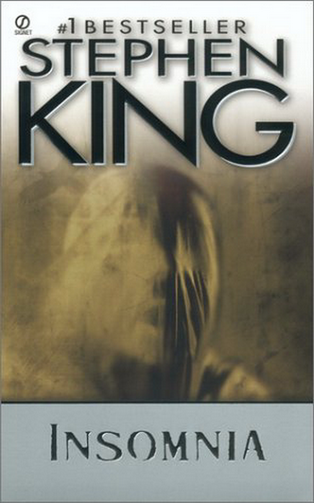
\includegraphics[width=0.85\linewidth]{pngStephen.png}}
\caption{}
\label{ris:image}
\end{figure}

\clearpage

(Insomnia) 1994

\textit{Посвящается Тэбби... и Эду Куперу, знакомому с правилами игры.
И в этом моей вины нет.}


\textbf{ПРОЛОГ} \textbf{УХОД СТРАЖА СМЕРТИ (I)}

\textit{Старость --- это остров, окруженный смертью.} Хуан Монтальво ``О
Прекрасном''

\textbf{1}

Никто --- и уж тем более доктор  Литчфилд --- не пришел к Ральфу Робертсу
и не сказал, что его жена умирает; в конце концов Ральфу все стало
ясно  и без слов. Время  между  мартом  и  июнем  показалось  ему
бесконечным,  суетным кошмаром  ---  утомительна  долгие  беседы  с
врачами,  нескончаемая  вереница вечеров, проведенных  у изголовья
Кэролайн  в клиниках, несметное количество поездок  в   лечебные
центры  других  штатов   для  проведения  специальных обследований
(слава  Богу,  что хоть стоимость  всех  этих  вояжей  покрыла
медицинская   страховка   Кэролайн),  собственные   изыскания  в
публичной библиотеке Дерри:  сначала  в  поисках ответов на то, что
специалисты могли проглядеть,  затем просто в поисках надежды  на  ту
последнюю соломинку,  за которую можно было бы ухватиться.

Эти четыре  месяца ассоциировались в  сознании  Ральфа с пьяным
угаром какого-то  безумного  карнавала  --- катающиеся  на  карусели
вскрикивают  от неподдельного  ужаса,  блуждающие  в зеркальном
лабиринте, в  его недрах,  а обитатели Аллеи  Ужасов фальшиво
улыбаются, но  в  их  глазах застыл жуткий страх. Ральф начал замечать
все эти  вещи в начале мая,  с приходом же  июня стал  понимать, что
так называемые светила медицины --- лишь жалкие знахари, а хор
подбадривающих  уверений  уже  не  мог  скрыть   того  факта,   что
из громкоговорителей доносится похоронный марш. Это был карнавал, все
правильно
- карнавал погибших душ.

В начале лета  1992  года  Ральф продолжал отгонять  от  себя
страшные видения  --- и еще более ужасную мысль, кроющуюся за ними,  -
но по мере того, как июнь  уступал место июлю, делать это  стало
практически невозможно.  Над центральным  Мэном распласталось самое
жаркое  лето начиная с 1971  года, и Дерри  кипел  в  котле
подернутого  дымкой  солнца,   влажности  и  дневной температуры,
превышающей 90 градусов по Фаренгейту. Городок  --- даже в лучшие свои
времена вряд ли претендующий на титул суматошного мегаполиса --- впал  в
полнейший  ступор, и  именно в этой  тишине Ральф  Робертс  впервые
услышал постукивание посоха Стража Смерти и понял, что в промежутке
между прохладной зеленью  июня и  прожаренной  неподвижностью июля
слабенькие шансы  Кэролайн превратились  в ничто. Ей суждено было
умереть. Может быть,  не этим летом --- врачи уверяли, что у  них  в
запасе еще осталась парочка трюков, и  Ральф не сомневался в этом,  -
но уж осенью или зимой  наверняка. Его давний и верный друг,
единственная женщина, которую он беззаветно любил, умирала.

Он пытался отбросить  саму мысль  о возможности подобного, называя
себя отвратительным старым идиотом, но в задыхающейся тишине этих
длинных знойных дней  Ральф  всюду  слышал  приближающееся
постукивание   неотвратимого  --- казалось, даже от стен исходило
дыхание смерти.

Но еще  сильнее  это постукивание слышалось в самой Кэролайн,  и,
когда она  поворачивала  к нему  свое  спокойное  бледное лицо ---  то
обращаясь  с просьбой сделать радио погромче, чтобы  послушать
передачу, пока она  чистит бобы на ужин, то спрашивая, не сходит ли он
в ``Красное яблоко'', чтобы купить ей эскимо, --- Ральф видел, что она
тоже знает об этом присутствии.

Он замечал  это знание в ее  темных глазах поначалу только тогда,
когда Кэролайн  смотрела на  него ясно и прямо,  но позже он научился
распознавать его  и  в  ее  затуманенном от  принимаемых
обезболивающих взгляде. К  тому времени поступь смерти стала уже
слишком явной, и, лежа  в  постели рядом  в эти  жаркие  летние ночи,
когда даже  простыня казалась десятипудовой, а все собаки Дерри выли
на луну, Ральф прислушивался к постукиванию Стража Смерти, стучащего
внутри Кэролайн, и ему казалось, что сердце его вот-вот разорвется от
горя  и  страха.  Сколько  еще придется  страдать  Кэролайн,  прежде
чем наступит конец? Сколько еще придется страдать ему самому? И как же
он сможет жить без нее?

Именно в этот  исполненный неизвестности  период  Ральф стал
совершать такие  длительные, изматывающие прогулки  в  жаркие, тягучие
летние сумерки, что  часто,  вернувшись  домой, не  находил в  себе
сил  даже поужинать. Он ожидал, что Кэролайн станет бранить  его за
то, что он  пропадает  Бог весть где, выговаривая: ``Наступит ли этому
конец, старый дурак? Ты же убьешь себя, если будешь разгуливать в
такую жару!'' Но она  не делала ничего подобного, и постепенно  пришло
понимание, что Кэролайн даже не отдает себе отчета в том, что
происходит в  действительности.  О том, что он отлучается ---  да, об
этом она знала. Но только  не о всех тех милях,  которые он одолевал,
и не о том, что,  возвращаясь домой, он нередко  дрожал  от
изнеможения  и  перегрева на солнце. Когда-то Ральфу  казалось, что
Кэролайн замечает  все, даже малейшее изменение  места пробора в его
прическе. Но все прошло; опухоль мозга лишила ее наблюдательности
точно так же, как вскоре она же лишит Кэролайн и жизни.

И  поэтому он бродил, наслаждаясь зноем, несмотря на то, что  иногда
от этого  все  плыло  перед  глазами,  а  в  ушах  появлялся
неприятный  звон; наслаждаясь в  основном потому, что от жары  у  него
звенело  в ушах; иногда целыми  часами в голове стучало  так  яростно,
что  Ральф  перестал  слышать приближающиеся шаги Стража Смерти
Кэролайн.

Он очень  много бродил по Дерри в тот знойный июль --- узкоплечий,
седой, лысеющий старик с огромными руками, все еще способными  к
тяжелой работе. Он брел от Уитчхэм-стрит  к Барренс-стрит, от
Канзас-стрит к  Нейболт-стрит, от Мейн-стрит к Мосту Поцелуев, но чаще
всего ноги сами уводили его на запад от Гаррис-авеню,  на которой  все
еще красивая  и  столь  любимая  им  Кэролайн Робертс в мареве
головной боли и морфия теперь доживала свой последний год.

Ноги уносили его в  сторону  аэропорта. Он шел по  дороге --- по пути
не попадалось ни  единого деревца, в тени  которого можно было  бы
укрыться от безжалостного  солнца, ---  пока  не начинал  чувствовать,
как ноги  перестают слушаться  и  подгибаются  от усталости,  и
только  тогда Ральф поворачивал обратно.

Частенько  он  отдыхал в  тени  площадки  для  пикников,  неподалеку
от служебного въезда на летное поле, ожидая, когда же придет второе
дыхание.

Вечерами   эта   площадка   становилась   местом   тусовки
подростков, наполненным грохотом рэпа, доносящегося из колонок
переносных магнитофонов, но в  дневное  время  она  служила
пристанищем группы людей,  которую  Билл Мак-Говерн, друг Ральфа,
окрестил Сборищем Старых Кляч Гаррис-авеню.

Старые  Клячи собирались здесь, чтобы поиграть в шахматы, выпить
джина, просто поболтать. Многих Ральф знал не один год (со Стэном
Эберли; например, он  учился  в школе),  и ему было уютно среди них...
Пока они не становились слишком назойливыми. Хотя вряд ли их можно
было назвать таковыми.  Это  были янки, воспитанные  в традициях
старой  морали,  полагающие,  что  то, о чем человек не считает нужным
говорить, является  только его  делом ---  и  ничьим больше.

Именно  в  одну  из  таких прогулок  Ральф  впервые осознал, что с
Эдом Дипно, проживающим с ним на одной улице, происходит что-то
неладное.

\textbf{2}

В  тот день  Ральф  прошел гораздо больше, чем обычно, возможно
потому, что грозовые облака стерли  солнце и над Дерри повеяло
прохладой. Ральф впал в  некое подобие  транса,  ни  о  чем не думал,
ни  на что не смотрел, кроме пыльных носков своих туфель, когда
четырехчасовой самолет из Бостона, идя на посадку,  стремительно
пролетел у него над головой, и хриплый вой реактивных двигателей
мгновенно вывел Ральфа из состояния апатии.

Он  смотрел,  как  самолет  пролетел  над  старой трамвайной  колеей
и ограждением,  отмечающим границы  аэропорта, смотрел, как тот
приблизился к взлетно-посадочной  полосе,  выпустив  голубые  струйки
дыма,  когда  шасси коснулись земли.  Ральф  взглянул  на часы,
отметив  про себя,  что самолет опоздал, затем посмотрел на
ярко-оранжевую крышу заведения Говарда Джонсона, располагавшегося
чуть дальше по дороге.  Да, в состоянии  транса он  прошел более  пяти
миль, даже  не  заметив,  как  быстро  пролетело время.  ``Время
Кэролайн'', --- пробормотал внутренний голос.

Да, да; время  Кэролайн.  Она  дома и  теперь отсчитывает минуты,
чтобы принять дарвон, а мужа нет, он ушел  так  далеко... Он почти  на
полпути  к Ньюпорту.

Ральф посмотрел вверх и  впервые по-настоящему увидел
пурпурно-синюшные молнии,  прорезающие небо над аэропортом. Вовсе не
обязательно, что  пойдет дождь,  по  крайней  мере не сейчас,  но
если  дождь  все-таки  пойдет,  он непременно  вымокнет,  а  укрыться
можно только  на  площадке для пикников у взлетно-посадочной полосы
N3, да и там лишь ветхая беседка, в которой никуда не деться от
неистребимого пивного запаха.

Ральф  еще раз взглянул на оранжевую крышу,  затем, сунув руку в
правый карман,  нащупал  пачку   счетов,  перехваченных  маленьким
серым  зажимом, подаренным Кэролайн к его шестидесятилетию.

Никто не удерживал  Ральфа от  того, чтобы дойти  до заведения
Говарда Джонсона и вызвать  такси... Кроме,  пожалуй, мысли о  том,
каким  взглядом может одарить  его таксист. Глупый старик,  могут
сказать глаза  в  зеркало заднего  обзора.  Глупый старик, зашедший
дальше,  чем следовало,  в  такой жаркий день. Если бы ты плавал, то
наверняка утонул бы.

``Это  паранойя, Ральф'',  ---  сообщил ему внутренний голос, и  теперь
его кудахтающий,  несколько покровительственный тон заставил Ральфа
вспомнить  о Билле Мак-Говерне.

Что ж,  может  и так. В  любом  случае он положится на удачу и
вернется домой пешком.

``А что, если это будет не просто дождь?

Прошлым  летом  в  августе выпал  такой град,  что повыбивало почти
все стекла в домах западной части города''.

-  Пусть  будет град,  --- произнес вслух Ральф. ---  Меня не так-то
легко подмять под себя.

Ральф  медленно  направился к городу,  вздымая  носками  туфель
легкие облачка  пыли. С запада,  оттуда,  где громоздились  тучи,
донеслись  первые раскаты грома. Солнце,  хотя  и  прикрываемое
тучами,  все еще отказывалось сдаваться   без  борьбы;   оно
окрашивало   края   надвигающихся   туч   в ослепительно-желтые  тона
и светило в случайные просветы  в  облаках, словно мощный софит.

Ральф испытывал радость от того, что  решил вернуться  пешком,
несмотря на усталость в ногах и ноющую боль в пояснице.

``По  крайней мере  хоть что-то,  ---  подумал  он. ---  Уж  сегодня ночью
я наверняка буду спать. Спать как убитый''.

Взлетное  поле ---  акры высохшей бурой травы с вросшими  в  нее
ржавыми трамвайными  рельсами, оставшимися здесь, словно следы давней
катастрофы, --- теперь  находилось  слева  от него. Вдалеке за
проволочной сеткой ограждения ему был  виден ``Юнайтед-747'' размером с
игрушечный самолетик, направлявшийся к  терминалу,  принадлежащему
двум  авиакомпаниям  ---  ``Юнайтед'' и  ``Дельта''.  Взгляд  Ральфа
остановился  еще на одном  средстве передвижения ---  это  был
автомобиль, отъезжавший от  главного  авиационного терминала,
расположенного на  этом  краю поля. Машина направлялась к служебному
выезду,  ведущему  на Гаррис-авеню.  В  последнее  время  Ральф
часто  наблюдал за въезжающими  и выезжающими оттуда  машинами;
площадка для  пикников, где  собирались Старые Клячи Гаррис-авеню,
находилась ярдах в семидесяти от этого места.

В приближающейся машине Ральф узнал ``датсун'',  принадлежащий Эду и
Элен Дипно... И вдруг понял, что автомобиль действительно движется.

Ральф ступил  на обочину,  не осознавая, что беспокойно сжимает
кулаки, пока маленькая  коричневая машина  подъезжала к  закрытым
воротам.  Для того чтобы открыть  ворота снаружи, необходима
специальная карточка-ключ; изнутри же  всю работу выполнял
фотоэлемент.  Однако последний установлен близко  к воротам, слишком
близко,  а  на скорости, с которой ехал ``датсун''... В самый последний
момент (или Ральфу это только показалось)  коричневая машина резко
затормозила, из-под колес взметнулось облачко голубого дыма, напомнив
Ральфу недавнюю  посадку  самолета,  и,  когда ворота  начали медленно
открываться, кулаки Ральфа разжались.

С  водительской  стороны  в окне  появилась  рука  и  яростно
замахала, пытаясь, очевидно, таким образом убедить ворота открыться
побыстрее.

Действие настолько абсурдное, что Ральф улыбнулся. Однако  улыбка
почти сразу умерла. Освежающий ветерок с запада, откуда надвигались
грозовые тучи, донес пронзительный крик водителя ``датсуна'':

- Сукин сын! Ублюдок! Поцелуй меня в задницу!

Пошевеливайся! Быстрее, дырка от бублика! Пугало огородное!

Крыса ты дохлая!

- Не может быть, что это Эд Дипно, --- пробормотал Ральф. Он снова
пошел, даже не осознавая этого. --- Не может быть.

Эд   работал   химиком-исследователем   в   лабораториях   Хокинга
во Фреш-Харборе, это  был  самый добрый  и учтивейший молодой
человек,  какого Ральф когда-либо встречал. Им с Кэролайн очень
нравилась Элен  --- жена Эда, а их малышку  Натали  они  просто
обожали.  Появление Натали  было  одним  из немногих  событий,
которое  могло   отвлечь  Кэролайн  от  ее   теперешнего состояния, и,
чувствуя это, Элен частенько брала девочку с собой. Эд никогда не
возражал.

Ральф знал о  существовании  мужей,  которых  раздражало, если их
жены бегали к старикам-соседям  всякий раз, когда младенец делал
что-то новое;  а уж если один из  этих стариков болен...  Ральфу
казалось, что  Эд не  сможет заснуть всю ночь, если вынужден будет
послать кого-то к черту, но...

- Ах  ты  старый козел!  Да  откроешься  ли ты  когда-нибудь?!
Вонючий ублюдок!

Но  голос   действительно   принадлежал   Эду.   Даже   на
расстоянии двухсот-трехсот ярдов трудно было ошибиться.

Теперь  водитель ``датсуна'' жал на акселератор, как ребенок,  давящий
на рычаг в автомате по измерению силы  в ожидании, что вот-вот
зажжется зеленая лампочка.  Из  выхлопной  трубы  вылетали  клубы
дыма.  Как  только  ворота приоткрылись для проезда, ``датсун'' с
грохотом проскользнул в  зазор, и Ральф наконец-то смог увидеть
водителя. Тот находился достаточно близко, так  что места для сомнений
не оставалось: все правильно, за рулем Эд.

``Датсун'' подпрыгивал на кочках немощеного отрезка дороги между
воротами и  шоссе.  Прозвучал  резкий  гудок,  и  Ральф  успел
заметить,  как  синий ``форд-рейнджер'',  направлявшийся   на  запад,
вильнул  в  сторону,  пытаясь избежать столкновения с  ``датсуном''.
Водитель пикапа слишком поздно  заметил опасность,  а  Эд, очевидно,
вообще  ничего не  увидел (лишь намного позднее Ральф стал
подозревать, что Эд специально пошел на таран ``форда'').

Взвизгнули  тормоза,  последовал  глухой  удар  крыла  ``датсуна'' о
бок ``форда''.  Пикап въехал  на  разделительную линию между  встречными
полосами шоссе.

Смятый капот ``датсуна'' раскрылся.  Стекло  разбитых  фар  посыпалось
на асфальт.  А  мгновение   спустя  обе   машины  замерли  посередине
дороги, переплетясь наподобие сюрреалистической скульптуры.

Ральф,  остолбенев,  наблюдал,  как  под  ``датсуном''  разливается
лужа бензина.  За  почти  семьдесят лет ему довелось быть  свидетелем
нескольких дорожных  столкновений, по  большей части незначительных, и
всякий раз  его поражала  стремительность происходящего  и то,
насколько  мало было  в этом драматизма. Как непохоже  на кино, где
камеры могут замедлять действие,  или на видео, где можно, если
возникнет такое  желание, снова и  снова смотреть, как машина
срывается с обрывала жизни это всего лишь серия размытых образов, за
которой  следует  быстрая  комбинация звуков:  визг  колес, глухой
звук корежущегося  металла,  рассыпной  дождь  стекла. А затем voila
- tout fini \footnote{Вот так --- все кончено (франц.). (Здесь и  далее
прим.  Переводчика).}.  Существовал даже некий протокол для событий
подобного рода:

Как  Человек  Должен  Вести  Себя При  Столкновении.  Конечно,
подобный ритуал  просто необходим, размышлял Ральф.  Каждый  день в
Дерри происходило около   дюжины  таких  столкновений,  а  уж  зимой,
когда  выпадал  снег  и становилось  холодней, возможно,  раза  в два
больше.  Выходишь  из машины, встречаешь  второго  участника  в  точке
столкновения  двух  машин  (где  те зачастую  еще  и  переплелись),
смотришь  и качаешь  головой.  Иногда ---  но вообще-то за  редким
исключением почти всегда ---  эта фаза  встречи  отмечена экспрессивной
перепалкой:  определяется  вина (довольно грубо),  мастерство каждого
водителя   ставится   под   сомнение,   звучат   угрозы  судебного
разбирательства;  однако Ральф  считал, что  на  самом  деле  водители
лишь пытаются сказать друг другу:

``Послушай, дурак, ты  же  напугал меня до смерти!`` Последним па в
этом коротком танце  являлся Обмен Священными Заверениями ---  обычно
именно в этот момент водители начинают брать под контроль свои
эмоции... Всегда ставя себе в заслугу то, что никто не пострадал, как
и в данном случае. Иногда водители даже обмениваются рукопожатием.

Ральф  приготовился  наблюдать  за всем  этим  со  своего  места  в
ста пятидесяти ярдах  от  точки столкновения, но как только
распахнулась дверца ''датсуна``, он понял, что  здесь все пойдет  иначе
-  инцидент не  только не закончился, но  ждет своего продолжения.  И
уж определенно  никто  не станет пожимать руки в финале этого
представления.

Дверца автомобиля не просто открылась --- она распахнулась.

Выскочивший на дорогу Эд  Дипно  замер  возле  своей машины, его
узкие плечи квадратом застыли на фоне темнеющих облаков. Он был в
потертых джинсах и  футболке,  и Ральф  отметил, что никогда прежде
не  видел Эда иначе, чем застегнутым  на  все  пуговицы.  И еще что-то
было  намотано вокруг шеи Эда: нечто белое и длинное. Шарф? Да, похоже
на шарф,  но кто же  станет надевать шарф в такую жару?

Эд стоял возле машины, глядя, казалось, во все стороны, кроме нужной.

Яростные повороты его  головы вызвали у  Ральфа  ассоциацию  с
петухом, оглядывающим свои владения в поисках захватчиков и чужаков.
Но что-то в этом сходстве вызвало беспокойство Ральфа. Никогда прежде
он  не видел Эда таким; скорее  всего, поэтому Ральф и встревожился,
однако его волновало и кое-что другое. Истина  же  была  проста:
никогда  и  никого Ральф не видел в  таком состоянии.

На западе прогрохотал гром, теперь уже громче. И ближе.

Мужчина,  выбравшийся  из ''форда``, вдвое,  а может, и втрое был
крупнее Эда. Огромный  живот  свисал над ремнем его зеленых рабочих
брюк;  (  белой рубашки  с распахнутым воротом выступали полукружия
пота размером с тарелку.  Бейсбольную  кепку  он сдвинул на  затылок,
чтобы лучше  рассмотреть нахала, врезавшегося  в  его  автомобиль.
Лицо  мужчины  с  тяжелой  челюстью  было смертельно бледным, лишь на
скулах горели яркие пятна, и Ральф подумал: ''Да он первый кандидат на
инфаркт. Находись я ближе, клянусь,  увидел бы красные прожилки  у
него на коже``, --- Эй! --- крикнул  толстяк, обращаясь к Эду. Голос,
вырвавшийся  из необъятной груди, звучал до абсурдности тонко,
пронзительно.

- Где это ты получал права?

Эд немедленно  повернул свою вертлявую  голову  в сторону голоса  -
как будто именно этого звука он  и ждал;  так летит самолет, ведомый
радаром,  и Ральф впервые увидел глаза Эда. Почувствовав, как в  груди
у него вспыхивает тревога, он побежал  в сторону столкновения. А в это
время  Эд направился  к Толстяку  в  пропитанной  потом  рубашке  и
бейсбольной  кепке.  Он  шел на негнущихся ногах дерганой походкой,
столь отличавшейся от его обычной легкой иноходи.

- Эд! --- крикнул Ральф, но  освежающий бриз, теперь уже  несущий с
собой холодок  скорого дождя, казалось,  отнес в сторону слова
прежде, чем те были произнесены. Эд  не обернулся. Ральф побежал
быстрее, забыв о ноющей  боли в ногах  и пояснице. В немигающих,
широко  открытых глазах Эда Дипно он увидел убийство. У Ральфа  не
было абсолютно,  никакого опыта обоснования подобных суждений,  но он
не думал, что в оценке такого взгляда можно ошибиться; так поглядывают
друг на друга бойцовые петухи при  нападении. --- Эд! Постой,  Эд!  Это
я, Ральф!

Тот даже не оглянулся, хотя теперь  Ральф  находился так близко, что
Эд просто  не мог не  слышать его,  несмотря  на  порывы  ветра.  А
вот Толстяк оглянулся, и Ральф заметил страх и неуверенность в его
глазах. Затем Толстяк снова повернулся к Эду и успокаивающе поднял
руки.

- Послушай, --- начал он, --- мы ведь можем поговорить... Это было все,
что он  успел  сказать. Эд стремительно сделал еще один шаг,
взмахнул кулаком --- казавшимся особенно белым в быстро  сгущающихся
сумерках --- и ударил Толстяка в его более чем внушительную  челюсть.
Звук  удара прозвучал, словно выстрел из детского духового ружья.

-  Сколько  человек  ты уже  убил? ---  спросил Эд. Толстяк прислонился
к своему пикапу, рот его был открыт, глаза выпучены. Тем же
быстрым, странным, скачущим шагом Эд  вплотную приблизился к Толстяку,
очевидно,  игнорируя тот факт, что водитель пикапа дюйма  на четыре
выше и фунтов на сто тяжелее его.  Эд снова ударил верзилу.

- Давай! Сознавайся, храбрец, --- сколько человек ты уже убил?

-  Эд  перешел  на  крик,  тут  же  заглушенный  первыми
внушительными раскатами грома.

Толстяк  оттолкнул Эда --- жест не агрессии, но простого испуга, ---  и
тот отлетел назад,  ударившись  о  покореженный капот  своего
''датсуна``,  однако сразу  же  ринулся  назад,  сжав кулаки,  готовый
наброситься  на Толстяка, съежившегося  возле своего ''форда`` в
съехавшей набекрень  кепке и выбившейся из  брюк  рубашке.  В  голове
Ральфа  пронеслось  воспоминание  ---  виденный давным-давно  немой
фильм,  в  котором  братья  Маркс  изображали туповатых маляров, --- и
внезапно он ощутил прилив  сочувствия  к  Толстяку, нелепому и
запуганному до смерти.

Эд  же  отнюдь  не выглядел нелепо.  Раскрытый  в широком  оскале рот
и немигающие глаза делали его еще более похожим на бойцового петуха.

- Я знаю, чем  ты  занимаешься, ---  прошипел  он  Толстяку. ---  Ты что
же думаешь,  это  все  игрушки?  Надеешься,  что тебе  и  твоим
дружкам-палачам удастся ускользнуть... И в этот момент подоспевший
Ральф, пыхтя как паровоз, положил руку на плечо  Эда. Жар  под  тонкой
футболкой обескураживал;  будто рука  его  легла  на раскаленную
печь, а когда  Эд  обернулся,  на какое-то незабываемое мгновение
Ральфу  показалось, что он  смотрит прямо  в бушующее пламя.  Никогда
прежде  не видел он  такой абсолютной, беспричинной ярости в
человеческих глазах, более того  ---  даже  не  подозревал,  что  такая
ярость возможна.

Импульсивно Ральф едва не отшатнулся,  но, подавив в себе это
желание, замер. Промелькнула мысль, что если сейчас он отступит, то Эд
набросится  на него, как взбесившийся пес. Нелепо, конечно. Эд был
химиком-исследователем, Эд  был  членом  литературного клуба  (из
тех,  кто изучает пудовые книги о Крымской  войне), Эд был мужем Элен
и отцом Натали. Черт, в конце концов, Эд был его другом...

... Вот только сейчас  перед ним стоял  вовсе  не Эд,  и Ральф
сознавал это.

И вместо  того, чтобы  отступить,  Ральф подался вперед, схватил Эда
за плечи  (такие   горячие  под  тонкой  тканью  футболки,  так
невообразимо, мучительно  обжигающие)  и стал поворачивать  его к
себе,  пока  Эд не отвел взгляд от Толстяка.

- Эд, прекрати! --- произнес Ральф громким,  сильным и уверенным
голосом, каким, по его глубокому убеждению,  только  и можно
разговаривать с  людьми, впавшими в истерику. --- Все нормально! Просто
успокойся!

Эд,  не сводивший остекленевших глаз с Толстяка, скользнул  взглядом
по лицу Ральфа. Не  такое  уж  большое  достижение, однако  Ральф
почувствовал некоторое облегчение.

- Что это с  ним? --- спросил Толстяк. ---  Вам не кажется, что он  сошел
с ума?

-  Уверен,  с  ним все в  порядке, ---  ответил Ральф, хотя вовсе  не
был убежден в чем-либо  подобном. Произнес он  это  сквозь зубы, не
сводя глаз с Эда.  Он не осмеливался отвести взгляд --- этот  контакт
казался  единственной зацепкой, позволяющей ему удерживать  парня,  но
зацепкой слишком хрупкой. --- Обычное  потрясение из-за случившегося.
Ему  нужно несколько секунд,  чтобы успо...

-  Спроси, что  там  у  него  под  брезентом! ---  внезапно закричал
Эд, указывая  через  плечо  Ральфа. Сверкнула  молния,  и на
какой-то  миг  мало заметные  шрамы  от юношеские прыщей  Эда стали
выпуклыми,  превратившись  в подобие странной рельефной карты.
Прогремел  гром. --- ''Эй, эй, Сьюзен  Дэй! --- пропел  Эд высоким детским
голосом, от которого у Ральфа мурашки поползли по телу. --- Сколько ты
убила детей``?

-  Да  никакое  у  него  не  потрясение,  ---  заключил   Толстяк.  -
Он сумасшедший. И когда  приедет  полиция, уж  я позабочусь, чтобы
его засадили куда следует.

Оглянувшись,  Ральф  увидел   над  кузовом  пикапа   голубой
брезент, закрепленный ярко-желтой бечевкой. Под брезентом угадывались
округлые формы.

-  Ральф? ---  прозвучал застенчивый  голос.  Он перевел взгляд  влево
и увидел  Дорренса  Марстеллара  ---  девяностолетнего старейшего
представителя Сборища Старых  Кляч  Гаррис-авеню  --- тот стоял  как
раз позади  грузовичка Толстяка.  Выдубленными  временем  руками
Дорренс  скручивал  и раскручивал книжку,  как бы проверяя  переплет
на крепость. Ральф  предположил, что  это сборник  стихов  -
единственное, что читал Дорренс. А может,  он и не читал вовсе;
возможно, ему просто нравилось держать книги в  руках и рассматривать
изящно сложенные строки.

- Ральф, в чем дело? Что происходит?

И  снова вспышка молнии,  пурпурно-белое ворчание.  Дорренс
неуверенно взглянул вверх, как бы желая там найти ответ на то, где он
находится, кто он такой и что именно  он  видит.  Ральф вздохнул.  -
Дорренс... ---  начал  было Ральф,  но  тут   Эд  бросился  на  него,
словно  дикий   зверь,  ненадолго утихомирившийся  только  для того,
чтобы собраться  с  силами.  Ральф  успел увернуться, толкнув Эда на
искореженный капот ''датсуна``.

Его охватила паника и неуверенность в том, как именно поступать
дальше.  Слишком  многое  происходило  одновременно. Ральф
чувствовал,  как  под его хваткой яростно  гудят мышцы рук Эда,  как
будто тот  умудрился  проглотить молнию, только что перерезавшую небо.

-  Ральф?  --- окликнул его  Дорренс  тем же тихим,  но  уже
озабоченным голосом. ---  На твоем месте я бы не стал больше
прикасаться к нему.  Я  и так уже не вижу твоих рук.

Отлично. Еще один сумасшедший. Как раз то, что нужно. Ральф взглянул
на свои кисти, затем на старика:

- Что ты плетешь, Дорренс?

-  Твои руки. Я их не вижу... --- Здесь не место для тебя,  Дор, -
почему бы тебе не убраться отсюда? При этих словах старик немного
приободрился.

- Да!  --- произнес  он тоном  человека, которому  только  что
открылась великая  истина.  ---  Именно  так  мне  и  следует
поступить. ---  Не успел он повернуться, как  снова  раздались  раскаты
грома, старик поежился и прикрыл своей книжкой голову. Ральф успел
прочитать оттиснутое ярко-красными буквами название: ''Предпочтения
щеголя``, --- Тебе следует  сделать то же самое, Ральф.  Не  стоит
вмешиваться  в дела  Лонг-таймеров \footnote{От  англ. long  -
длинный, продолжительный и time --- время. Неологизм, используемый С.
Кингом   в  его  своеобразной   философской  концепции   бытия.
Далее встречаются shorttimer (короткий, краткосрочный),  all-timer (от
англ. all --- весь, все) и old-timer (от англ.  old --- старый).}. От
этого  можно только пострадать.

-  Что  это  ты... Не  дав Ральфу  договорить,  Дорренс  развернулся
и поковылял в направлении  площадки  для пикников, седые  волосы,
напоминающие пушок новорожденного, ерошило ветром --- спутником
надвигающейся грозы.

Итак, одна проблема решена, но успокаиваться было рановато.

Дорренс  временно отвлек внимание Ральфа от Эда, и теперь  парень
снова злобно поглядывал на Толстяка.

- Грязный ублюдок! --- выкрикнул он. --- Имел я твою мать!

Толстяк насупился:

- Что-о?

Взгляд Эда снова метнулся к Ральфу --- кажется, теперь он узнал соседа.
- Спроси-ка,  что  у него там  под брезентом?  ---  закричал Эд. -
Оаставь этого убийцу показать тебе это!

Ральф взглянул на Толстяка: --- И что же у вас  там такое? --- А тебе
какое дело?   ---   парировал   тот,   стараясь   придать  голосу
язвительность  и агрессивность.  Он попытался  поймать  взгляд Эда
Дипно и  на всякий  случай сделал два робких шажка в сторону.

-  Мне никакого, а вот ему это  нужно, ---  ответил Ральф, слегка
поведя головой в сторону Эда. --- Просто помоги мне успокоить его,
ладно?

- Ты его знаешь?

- Убийца! --- снова крикнул  Эд и на этот раз так рванулся из рук
Ральфа, что тому пришлось отступить на шаг. Ко всему прочему
происходило что-то еще.  Ральфу  показалось,  что пугающе пустой
взгляд Эда  становится  осмысленным.  Теперь  в  его глазах было
больше Эда,  чем прежде... Или,  возможно,  Ральф просто принимал
желаемое за действительное. -Убийца!

Убийца младенцев!

- Господи,  бред собачий,  --- пробормотал Толстяк, но, подойдя к
кузову, развязал  один из  узлов и  отвернул угол  брезента. В
кузове стояло  четыре деревянных  бочонка с  надписью ''ОТ  СОРНЯКОВ``.
- Органическое удобрение,  --- пояснил Толстяк, переводя взгляд  с Эда
на  Ральфа, затем  снова  на Эда. Он дотронулся до  козырька  кепки с
эмблемой  общества  садоводов. --- Целые  дни напролет я вожусь с
цветочными клумбами в Джунипер-Хилл. Это психиатрическая лечебница на
окраине Дерри... Где тебе не мешало бы отдохнуть, дружок.

- Удобрение? --- произнес Эд, как бы  спрашивая самого себя.  Левой
рукой он потер висок. --- Удобрение? --- Он спрашивал  так, будто речь
шла о  простом, но вызывающем сомнение научном открытии.

- Удобрение, --- подтвердил Толстяк, поворачиваясь к Ральфу, и добавил:

- У этого парня с головой не все в порядке. Вы согласны?

- Просто  он сбит  с  толку,  ---  смущенно ответил  Ральф, наклоняясь
к кузову. Он  постучал по крышке  бочонка, затем повернулся к Эду. -
Бочонки с удобрением, --- сказал он. --- Теперь ты доволен?

Ответа  не  последовало.  Медленно  подняв  вверх правую руку, Эд
стал тереть второй висок. Он был похож на страдающего невыносимой
мигренью.

- Теперь ты доволен? --- Ральф мягко повторил свой вопрос.

Эд на мгновение прикрыл глаза, а когда снова открыл их, Ральф заметил
в них влажный блеск, словно от подступивших слез. Эд осторожно
облизнул языком сначала  один  уголок рта, затем другой. Кончиком
шелкового шарфа  он вытер лоб, при этом Ральфу стали видны вышитые по
краю шарфа китайские иероглифы.

- Мне кажется... Возможно... --- начал было Эд, но тут же замолчал.

Зрачки  его снова расширились,  и взгляд приобрел то прежнее
выражение, которое так не понравилось Ральфу. --- Дети! --- резко
выкрикнул он. -Ты слышишь меня? Младенцы!

Ральф снова прижал его  к машине  уже  в третий  или  четвертый раз
он сбился со счета.

- О  чем ты говоришь,  Эд? --- Внезапно  в голове  у Ральфа вспыхнуло:
- Что-то случилось с Натали? Ты беспокоишься о Натали?

Хитроватая, коварная  ухмылка  искривила  губы  Эда.  Он посмотрел
мимо Ральфа на Толстяка:

- Значит, удобрение? Что ж,  если это так, ты ведь не станешь
возражать и откроешь один из бочонков?

Толстяк беспокойно взглянул на Ральфа.

- Парню нужен доктор, --- промямлил он.

- Не исключено. Но мне показалось, что он успокаивается... Можешь ли
ты открыть один из бочонков? Возможно, от этого ему станет легче.

- Конечно, в чем проблема? Назвался груздем --- полезай в кузов. Еще
один всплеск молнии, еще один раскат грома ---  на этот раз  будто
прокатившийся по всему  небу, --- и первая холодная капля дождя упала на
потную шею  Ральфа. По левую руку от него  Дорренс Марстеллар, стоя
возле площадки для  пикников с книгой в руках, встревоженно смотрел на
всю троицу.

- Кажется, сейчас  хлынет как  из ведра, --- поежился Толстяк,  --- а  я
не могу допустить,  чтобы  все  это  добро  намокло, иначе  начнется
химическая реакция.  Так  что  смотрите  быстрее.  --- Просунув  руку
между бочонками, он достал  ломик. --- Должно быть,  я  такой же
сумасшедший,  как и он, раз делаю это,  ---  сообщил водитель  Ральфу. -
Я  ехал домой, думая о своем. А он сбил меня.

- Давай, действуй, --- перебил его Ральф. --- Это займет не больше
секунды.

- Да,  ---  кисло протянул Толстяк, поддевая плоским концом ломика
крышку ближайшего бочонка, --- но воспоминаний хватит на всю
оставшуюся жизнь. Именно в этот  момент  снова  прогрохотал  гром,  и
Толстяк не услышал  того,  что произнес Эд Дипно. Ральф, однако,
услышал, и у него свело желудок.

- Эти бочонки набиты мертвыми младенцами, --- поделился своим мнением
Эд.
- Вот увидишь.

В  голосе Эда было  столько убежденности,  что  пока  Толстяк
открывал крышку  бочонка, Ральф почти ожидал  увидеть переплетенный
клубок рук, ног и маленьких безволосых головок. Вместо  этого его
взору предстала смесь белого и коричневого порошка. Из бочонка пахнуло
то ли торфом, то ли химикатами.

- Ну что? Теперь ты удовлетворен? ---  спросил Толстяк, снова обращаясь
к Эду. --- В конце концов,  я же не Рей Джуберт и  не этот маньяк
Дамер. Так что скажешь?

На лице  Эда появилось виноватое  выражение,  а  когда в очередной
раз прогремел  гром,  он  весь  как-то  съежился. Наклонившись
вперед,  молодой человек протянул руку к бочонку, затем вопросительно
взглянул на Толстяка.

Ральфу показалось, что тот кивнул почти сочувственно:

-  Конечно,  потрогай, я не возражаю. Но если пойдет  дождь,  когда
ты будешь держать это  в руке, запляшешь не  хуже  Джона Траволты
\footnote{Известный голливудский киноактер и танцор.}. Оно сильно
жжет.

Эд запустил руку в бочонок, зачерпнул немного смеси и просеял ее
сквозь пальцы. Он  ошеломленно посмотрел  на  Ральфа  (была  в его
взгляде  и  доля замешательства), а затем погрузил руку по самый
локоть.

- Эй, --- испуганно закричал Толстяк. --- Это же не коробка с крекерами!
На мгновение хитрая  ухмылка  снова  появилась  на  лице  Эда -
она, казалось, говорила:  ''Я  знаю  трюк  и получше  этого``. ---  а
затем  ее  опять сменила растерянность, когда он не обнаружил ничего,
кроме удобрения.

Эд вытащил руку из бочонка  --- испачканную, пахнущую химической
смесью.  Еще  одна  молния  сверкнула   над   взлетным   полем,  за
ней   последовал оглушительный раскат грома.

- Сотри это, пока не пошел дождь, --- посоветовал Толстяк.

Через опущенное стекло своего  ''форда``  он достал пакет салфеток,
вынул пару и передал Эду --- тот, словно во сне, стал стирать смесь с
рук. А Толстяк в  это  время  закрыл  крышку, вставив  ее на место
одним ударом  огромного кулачища,  и  бросил быстрый  взгляд  на
темнеющее небо''  Когда Эд  коснулся рукава его белой рубашки, мужчина
напрягся, беспокойно взглянув на парня.

- Кажется, я должен извиниться, --- произнес Эд, и впервые тон его
голоса показался Ральфу абсолютно чистым и разумным.

-  Ну ты  и весельчак, --- облегченно хохотнул  Толстяк, опуская
покрытый полиэтиленовой пленкой  брезент  и завязывая  узлы  серией
быстрых,  умелых жестов.  Наблюдая за  ним,  Ральф  подумал о том,
каким  же хитрым  воришкой оказалось время. Когда-то и он мог с такой
же легкостью и проворством вязать узлы.  Он и сейчас мог проделать
подобное, однако теперь ему понадобилось бы минуты две и, возможно,
три его самых любимых ругательства.

Толстяк похлопал  по брезенту,  а затем  повернулся,  скрестив  руки
на своей необъятной груди.

- Вы видели столкновение? --- обратился он к Ральфу.

-  Нет, --- моментально  отреагировал  тот.  Ральф не имел  ни
малейшего представления,  почему лжет, но решение  пришло
мгновенно. --- Я наблюдал, как приземляется ``Юнайтед''.

К его  превеликому  удивлению, яркие пятна на щеках Толстяка
проступили еще резче. ``Ты тоже наблюдал за ним! --- внезапно подумал
Ральф. --- И не только за посадкой, иначе ты не стал бы так отчаянно
краснеть...  Ты  смотрел и  на то, как самолет выруливает к
терминалу''.

За этой мыслью последовало полнейшее откровение. Толстяк считал, что
он сам виноват в столкновении, и опасался, что полицейские, которые
прибудут на место аварии, станут  придерживаться  той  же точки
зрения.  Он наблюдал за самолетом и не  заметил  машины Эда,
стремительно  выехавшей  из  ворот  на дорогу.

- Послушай, я действительно сожалею, --- искренне произнес Эд; вид у
него был не просто виноватый --- парень являл собой сплошное уныние.

Ральф внезапно поймал себя на мысли о том, в какой степени он
доверяет своим глазам и  действительно  ли понимает хоть немного  из
того, (Эй,  эй, Сьюзен Дэй) что произошло здесь... И кем, в конце
концов, была Сьюзен Дэй?

-  Я ударился  головой  о  руль,  --- говорил  в это  время Эд,  ---  и
мне кажется... Понимаешь, у меня что-то заклинило.

- Думаю, так оно и было. --- Почесав затылок, Толстяк посмотрел на
низкое темное небо, затем снова на Эда. --- Хочу кое-что предложить
тебе, приятель.

- Да? Что именно?

-  Давай  просто обменяемся именами и номерами телефонов,  вместо
того чтобы  ввязываться  во  все это дерьмо  со страховками.  А
затем разъедемся каждый в свою сторону.

Эд  неуверенно  взглянул на Ральфа, пожавшего плечами, а затем снова
на мужчину в кепке.

-  Если  в  дело  вмешается полиция, ---  продолжал  Толстяк,  ---  у
меня возникнет множество проблем. Во-первых, они сразу выяснят, что
прошлой зимой я тоже оказался участником столкновения и теперь  езжу
по временным правам.  Поэтому они постараются насолить мне.
Понимаешь, о чем я говорю? --- Конечно,
- ответил Эд. --- Но в этом столкновении виноват только я.

Видишь ли, я ехал слишком быстро...

- Возможно, столкновение еще не самое главное, --- перебил  его
Толстяк, недоверчиво  оглядываясь на приближающийся грузовик, потом
снова взглянул на Эда и заговорил  более настойчиво: --- Из машины
вытекло немного бензина, но я уверен, что  ты сможешь доехать домой...
Если  ты  житель этого городка. Ты ведь живешь здесь?

- Да, --- ответил Эд.

- А я оплачу ремонт, полсотни баксов, идет?

Новое  откровение  посетило  Ральфа;  существовала  одна-
единственная причина, объясняющая  внезапный поворот в поведении
незнакомца от грубости к заискиванию.  Автокатастрофа  прошлой зимой?
Возможно. Но Ральф  никогда  не слышал о такой вещи, как временные
права, и считал, что  это почти наверняка вранье.  Старина  Садовник
разъезжал   без  прав.  Ситуацию   же  усложняло следующее: Эд говорил
правду --- столкновение было полностью на его совести.

- Если же мы разъедемся подобру-поздорову,  --- продолжал  Толстяк, -
мне не придется снова объясняться с  полицией, а тебе
растолковывать,  почему ты выскочил  из  своей машины  и  накинулся
на  меня,  как  разъяренный зверь, утверждая, что мой грузовичок набит
мертвыми младенцами.

- Неужели я действительно говорил такое? --- ошеломленно спросил Эд.

- Конечно, --- мрачно подтвердил Толстяк.

Слегка картавя, голос с французским акцентом произнес:

- Все в порядке, ребята? Никто не пострадал?.. Эй, Ральф! Это ты?

За рулем подъехавшего грузовика с надписью ``ХИМЧИСТКА ДЕРРИ'' сидел
один из  братьев  Вашон, проживавших  в Олд-Кейп.  Скорее  всего,
Триггер,  самый младший.

- Это я, --- ответил Ральф и, не отдавая себе отчета в происходящем -
все его действия сейчас  подчинялись  инстинкту, --- подошел к
Триггеру, обнял за плечи и повел парня в направлении его машины.

- С ними все в порядке?

-  Да,  да, --- ответил Ральф. Оглянувшись назад, он  посмотрел на Эда
и Толстяка, склонившихся над кузовом  ``форда''. ---  Немного помяли
машины.  Они сами во всем разберутся.

- Хорошо, хорошо, --- благодушно согласился  Триггер  Вашон. --- А как
твоя милая женушка, Ральф?

Ральф вздрогнул.

- Господи!  ---  воскликнул он и взглянул на часы, надеясь, что сейчас
не больше пяти двадцати --- пяти тридцати. Однако было уже  без десяти
шесть. На двадцать минут  позже того времени, когда  он должен
принести Кэролайн чашку бульона с половиной сэндвича. Она, конечно же,
волнуется. А вспышки молнии и аккомпанемент грома, разносящийся по
пустому дому, испугают ее еще больше. И уж если дождь действительно
пойдет, она не сможет  закрыть  окна;  у нее не хватало сил даже
поднять руку.

- Ральф? --- окликнул его Триггер. --- Что-нибудь случилось?

-  Да  так, ничего, --- ответил  старик.  ---  Просто я загулялся  и
совсем потерял  счет времени. А  затем произошло  это столкновение,
и... Ты можешь подвезти меня домой, Триг? Я заплачу тебе.

- Не надо мне никакой платы, --- возразил Триггер. --- Нам по пути.

Садись, Ральф. Ты думаешь, с этими парнями все будет нормально? Они
тут ничего такого не натворят?

- Нет, --- ответил Ральф. --- Мне так не кажется. Подожди секунду.

- Конечно.

Ральф подошел к Эду.

- Вы договорились?

- Да, --- ответил Эд. --- Мы уладим все частным образом. Почему бы и нет?

В конечном счете все сводится к кучке разбитого стекла.

Теперь  Эд  говорил  в своей обычной манере, и здоровяк в белой
рубашке внимал  ему  почти  с уважением. Ральфа все еще  не  покинули
недоумение  и тревога по поводу всего, что произошло здесь, но он
решил позволить событиям идти своим чередом. Ему очень нравился Эд
Дипно, но в этот июль его заботило совсем иное; его волновала Кэролайн
и то  странное существо,  которое начало стучать в стенах его спальни
- и внутри нее глубокой ночью.

-  Отлично,  ---  сказал  он  Эду.  ---  Тогда  я  поеду  домой. Мне
нужно приготовить ужин для Кэролайн, я и так запоздал.

Он уже  повернулся,  намереваясь уйти, но  тут  Толстяк остановил
его, протягивая руку.

- Джон Тэнди, --- представился он.

- Ральф Робертс. Рад познакомиться.

Тэнди улыбнулся:

- Сомневаюсь, что  при подобных  обстоятельствах... Но  я
действительно рад, что вы вовремя оказались поблизости. В какой-то
момент мне показалось, что мы поубиваем друг друга.

``Как и мне'', --- подумал, но не сказал Ральф. Он посмотрел  на  Эда,
его встревоженный взгляд задержался на  непривычной  футболке,
прилипшей к тощей груди, и на белом шелковом шарфе с красными
китайскими иероглифами.

Ему  не понравилось выражение глаз Эда, когда  их  взгляды
встретились; возможно, Эд еще не полностью пришел в себя.

- Ты уверен, что с тобой все в порядке? --- поинтересовался Ральф.

Ему  хотелось  уйти, оказаться  рядом  с Кэролайн,  но  неясное
чувство удерживало его --- ощущение того, что ситуация далеко не такая,
какой кажется.

- Все нормально, ---  быстро ответил Эд, одаривая Ральфа широкой
улыбкой, не  затронувшей, однако, его  темно-зеленых глаз, взгляд
которых внимательно изучал  Ральфа, словно спрашивая, многое  ли тот
увидел... И что он (Эй, эй, Сьюзен Дэй) будет помнить впоследствии.

\textbf{3}


Внутри грузовика Триггера Вашона пахло чистым, свежевыглаженным
бельем: аромат, который почему-то всегда ассоциировался в  сознании
Ральфа с запахом только  что  испеченного хлеба.  В машине  не  было
сиденья для  пассажира, поэтому Ральф ехал стоя,  ухватившись одной
рукой  за ручку дверцы, а другой держась за корзину с бельем.

- Послушай, все-таки там произошло что-то странное, --- произнес
Триггер, поглядывая в зеркало заднего обзора.

- Да я и половины не видел, --- пожал плечами Ральф.

- Одного из них я знаю. Дипно.  У него хорошенькая жена. Мне  он
всегда казался приятным человеком.

- Сегодня он сам на себя не похож, --- покачал головой Ральф.

- Ему что, оса под хвост попала?

- Целый рой.

Триггер засмеялся, хлопая ладонью по вытертому черному пластику руля.
- Целый  рой! Отлично сказано! Надо запомнить!  --- Триггер вытер
слезящиеся  от смеха глаза носовым платком размером со скатерть. --- Мне
показалось, что этот мистер Дипно выехал из служебных ворот.

- Так оно и было.

- Для этого нужен пропуск, --- заметил Триггер. ---  Как ты думаешь,
откуда у него пропуск?

Ральф, нахмурившись, поразмышлял, затем покачал головой:

- Не знаю. Мне и в голову это не  пришло.  Надо будет спросить  у
него, когда увидимся.

- Обязательно, ---  кивнул головой Триггер. ---  И поинтересуйся,  как
там поживают его осы. ---  Это  вызвало  у  него  новый взрыв  смеха,
что, в  свою очередь, повлекло за собой появление гигантского платка.

Когда они въехали на Гаррис-авеню, гроза наконец-то разразилась.

Града не  было,  но дождь  превратился в летний  ливень такой силы,
что Триггеру пришлось снизить скорость до черепашьего шага.

- Ух ты! --- уважительно  воскликнул  он. ---  Похоже  на ливень 1985
года, когда улицы половины города превратились в каналы. Помнишь,
Ральф?

- Да, --- ответил Ральф. --- Надеюсь, подобное не повторится.

- Не должно, --- согласился Триггер, с улыбкой вглядываясь в дорогу
через залитое дождем стекло. --- Они отремонтировали дренажную
систему.

Красота!

От  холодного  дождя и  тепла  в  кабине нижняя  часть  лобового
стекла запотела. Машинально Ральф нарисовал пальцем на запотевшем
стекле следующее:\footnote{изображение  двух  иероглифов}  ---  Что  это?  -
поинтересовался Триггер.

- Я и сам точно не знаю. Похоже на китайские иероглифы, да?

Почти такие же вышиты на шарфе Эда Дипно.

- Они  мне  что-то  напоминают, ---  снова взглянув  на рисунок,
произнес Триггер. Затем хмыкнул,  щелкнув пальцами. --- Послушай-ка:
по-китайски я могу сказать только одно: му-чу-чан-пэн!

Ральф улыбнулся, но вряд ли ему хотелось смеяться. И причиной тому
была Кэролайн. Происшедшее отвлекло его, но теперь он уже не мог не
думать о жене
- его воображение рисовало распахнувшиеся окна, развевающиеся шторы,
похожие на руки призраков, дождевые лужи в комнатах.

- Ты по-прежнему живешь в двухэтажном доме напротив ``Красного
  яблокаri?

- Да.

Триггер подъехал  к  тротуару, из-под  колес  грузовика  вырвались
два огромных  веера  воды. Дождь  лил как  из ведра.  В  небе
вспыхивали молнии, громыхал гром.

- Не  переждать ли тебе немножко здесь со мной?  --- предложил Триггер.
- Думаю, минуты через две ливень кончится.

- Да нет, не стоит. ---  Вряд ли Ральфа можно было удержать в машине
хоть на секунду дольше, даже наручниками. --- Спасибо, Триг!

- Вот это льет! Возьми хоть кусок пленки --- прикроешь им голову!

- Да нет, не стоит, спасибо. Я просто... Ральф не смог закончить
фразу, его состояние было  близко к панике. Он открыл дверцу
грузовика и выпрыгнул, по  щиколотки погружаясь в холодную воду. Не
оглядываясь, Ральф помахал  на прощание Триггеру и поспешил к дому,
который он и  Кэролайн делили  с Биллом Мак-Говерном, на ходу
нащупывая в кармане ключи от входной двери. Добежав до крыльца, он
понял,  что ключи  ему не нужны --- дверь  оказалась  распахнутой.
Билл,  проживавший  на  первом этаже, часто  забывал  запереть ее,  и,
решил Ральф,  лучше   уж  считать,  что  это  Билл  оставил  дверь
открытой,  чем представить, как Кэролайн вышла на улицу в поисках его
и попала под дождь. О возможности подобного страшно было даже
подумать.

Ральф  поспешил  в  сумрачный  коридор  первого этажа, зажмурившись
от оглушительного  раската  грома,  и  кинулся к  лестнице.  Там  он
мгновение помедлил,  ухватившись рукой  за перила и  слушая, как  вода
стекает  с  его промокших брюк  и рубашки  на  деревянный  пол. Затем
стал  подниматься ему хотелось взбежать наверх, но силы  его  были
истощены долгой ходьбой. Сердце бешено колотилось в груди,  промокшие
туфли висели на ногах пудовыми гирями, и почему-то перед глазами
встала  картина того, как Эд Дипно вертел головой, выйдя из своего
``датсуна'',  --- напряженные,  яростные  рывки, делавшие  парня похожим
на задиристого петуха перед боем.

Как  всегда  громко  скрипнула  третья ступенька, и  сразу  же
наверху раздались  торопливые  шаги.  Но они  не вызвали облегчения,
потому  что не принадлежали  Кэролайн,  он  сразу понял это,  а  когда
Билл  Мак-Говерн  с бледным,  озабоченным  лицом и  в  своей
неизменной  панаме  склонился  над перилами,  Ральф  даже не
удивился. Разве  не  чувствовал  он  всю обратную дорогу, что что-то
случилось? Чувствовал. Но  в данных обстоятельствах  вряд ли это можно
было  назвать предчувствием. Он  пришел  к открытию, что, когда
события достигают определенной степени  напряженности, их  уже
невозможно ни исправить,  ни  изменить. Ральфу  казалось,  что в той
или иной степени  он всегда  знал об этом.  Единственное,  о чем  он
никогда не  догадывался, то, насколько длинна может быть эта черная
полоса.

- Ральф! --- крикнул  Билл. ---  Слава Богу!  У  Кэролайн...  Думаю,
что-то вроде апоплексического удара. Я только что вызвал ``скорую
помощь''.

Ральф понял, что в конце концов он  может пробежать  оставшиеся
ступени лестницы.

\textbf{4}


Кэролайн лежала в дверном проеме кухни, разметавшиеся волосы
прикрывали лицо. Ральф подумал, что  в этом есть что-то особенно
ужасное; она выглядела так неряшливо, а  уж неряшливой Кэролайн
никогда не хотела быть. Опустившись на  колени,  Ральф  убрал  волосы
с ее лба и глаз.  Кожа  Кэролайн  под его пальцами была столь же
холодной, как и его промокшие туфли.

-  Я хотел  перенести ее на диван, но  для  меня  она очень тяжелая,
- пояснил Билл, нервно теребя смятую панаму. --- Моя спина, ты же
знаешь...

- Я знаю, Билл, все нормально, --- успокоил его Ральф.

Просунув руку под  спину  Кэролайн, он поднял жену.  Ему она  вовсе
не казалась тяжелой, наоборот  ---  легкой, почти такой  же легкой, как
созревший одуванчик, готовый в любой момент отдать свое семя ветру.

- Хорошо, что ты оказался рядом.

- Я как раз собирался уходить, --- рассказывал Билл, идя вслед за
Ральфом в гостиную и по-прежнему теребя  панаму. Это  заставило
Ральфа  вспомнить о старике Дорренсе Марстелларе с его книжкой стихов.
``На твоем месте я не стал бы больше прикасаться к нему, Ральф, -
сказал  старик Дорренс. --- Я и так уже не вижу твоих рук''.

- Я выходил, когда услышал грохот... Должно  быть,  это она упала...
- Билл оглядел темную от грозы гостиную, лицо его было одновременно
безумным и каким-то алчным, глаза,  казалось, искали  то, чего
здесь не было. Затем его взгляд прояснился.  ---  Дверь? ---  воскликнул
он. ---  Клянусь, она  до сих  пор открыта. Дождь проникнет внутрь! Я
сейчас вернусь, Ральф.

Он  поспешил  к  выходу.  Ральф  вряд  ли  заметил  это;  день
приобрел сюрреалистические аспекты ночного кошмара. Постукивание
усилилось. Он слышал этот звук отовсюду, даже гром не мог заглушить
его.

Уложив Кэролайн на диван, Ральф склонился  над  ней. Дыхание жены
было быстрым, поверхностным, а запах изо  рта ---  отвратительным.
Однако Ральф не отодвинулся.

- Держись,  милая, ---  попытался ободрить он ее,  беря за руку --- та
была почти такой же холодной, как и ее лоб, --- и нежно поцеловал.
-Просто держись.  Все хорошо, хорошо.

Но хорошо не было. Постукивание означало, что ничего не было хорошо.

И стучало не в стенах --- да никогда там ничего не стучало, --- это
стучало в его жене. В Кэролайн. Это было  в его  любимой  женщине; она
ускользала от него, и что он будет делать без нее?

- Держись, --- повторил Ральф. --- Ты слышишь меня? --- Он снова поцеловал
ее руку,   затем  прижал  к  своей  щеке,  а  когда  услышал
завывание  сирены приближающейся ``скорой помощи'', заплакал.

\textbf{5}


Кэролайн  очнулась  в  машине, на  бешеной  скорости  мчащейся по
Дерри (снова выглянуло солнце, от асфальта  шел  пар), и начала нести
такой бред, что Ральф подумал было,  что его жена потеряла  рассудок.
Затем, когда речь Кэролайн стала приобретать осмысленность,  с ней
случился второй припадок, и Ральфу вместе с одним из врачей пришлось
держать ее.

Поговорить  с Ральфом  в комнату ожидания на  третьем  этаже  пришел
не доктор  Литчфилд,  а  доктор  Джамаль,  невропатолог.  Тихим,
успокаивающим голосом он сообщил,  что состояние Кэролайн
стабилизировалось, но ее оставят в клинике на ночь, а утром ее можно
будет увезти домой. К тому же необходимо купить  некоторые
медикаменты  ---  таблетки,  правда,   дорогие,  но   очень эффективные.

- Не  следует  терять  надежды, мистер  Робертс, ---  попытался
успокоить Ральфа доктор Джамаль.

- Конечно,  ---  согласился тот. --- А подобные приступы будут
повторяться, доктор Джамаль?

Врач улыбнулся. Спокойствие его тона усиливал мягкий индийский акцент.

И хотя  доктор  Джамаль  не сказал прямо, что  Кэролайн умирает, он
так близко подошел к истине, как не осмелился сделать это ни один
другой человек в течение всего томительного года, когда Кэролайн
боролась за свою жизнь.

Новое   лекарство,   сказал   доктор  Джамаль,  возможно,
предотвратит повторные  приступы,  но  болезнь   достигла   такой
стадии,  когда  любые предсказания  могут  оказаться  ошибочными.  К
сожалению,  несмотря на  все принятые медиками меры, опухоль
продолжает увеличиваться.

-  Могут  возникнуть  проблемы  с  координацией  движений,  -
стараясь говорить как можно спокойнее, закончил доктор Джамаль. --- К
тому же я заметил некоторое ухудшение зрения.

- Могу ли я провести ночь возле нее? --- спросил  Ральф. --- Кэролайн
будет спать лучше, зная, что я рядом. --- Помолчав, он добавил: --- Как
и я.

- Конечно! --- доктор Джамаль повеселел. --- Отличная идея!

- Да, --- угрюмо согласился Ральф. --- Я тоже так считаю.

\textbf{6}


Итак, он сидел рядом со  спящей женой, прислушиваясь к  постукиванию,
и думал: ``Очень  скоро --- может быть, осенью или зимой я снова окажусь
с ней в этой комнате''. Мысль казалась пророческой. Склонившись, Ральф
положил голову на простыню, прикрывавшую грудь жены, Он не хотел
больше плакать, но не смог сдержать слез. Постукивание. Такое громкое
и непрестанное.

``Хотелось бы мне схватиться  с тем Стражем, что производит этот звук,
- подумал он. --- Я разорвал бы его в клочья. Бог мне свидетель'', После
полуночи Ральф задремал в кресле, а  когда проснулся, воздух  стал
прохладнее, чем во все предшествующие  недели,  и бодрствующая
Кэролайн смотрела на него ясными глазами.  Она  казалась  вполне
здоровой. Ральф  отвез ее  домой и  старался делать все,  чтобы
последние месяцы она прожила как можно комфортнее. Прошло много
времени, прежде чем он снова вспомнил об Эде Дипно.

Пока лето переходило в осень, а  осень в последнюю зиму Кэролайн,
мысли Ральфа были заняты Стражем Смерти,  который,  казалось, стучал
все  громче и громче, хотя и медленнее.

Но со сном у него никаких проблем не возникало. Это пришло позже.

\textbf{ЧАСТЬ ПЕРВАЯ} \textbf{ЛЫСОГОЛОВЫЕ ДОКТОРА-КОРОТЫШКИ}


\textit{Между  теми,  кто может  спать, и теми,  кто не может,
пролегает целая бездна.}

\textit{Это одно из самых огромных разделений человеческой расы.}

Айрис Мердок

``Монахини и солдаты''

\textbf{Глава первая}

\textbf{1}


Спустя  месяц  после  смерти жены Ральф  Робертс впервые в  жизни
стал страдать бессонницей.

Поначалу проблема  казалась  не  слишком  серьезной,  однако
положение постоянно  ухудшалось. Спустя полгода  после первого
нарушения  в его прежде ничем не примечательном цикле сна и
бодрствования Ральф достиг такой степени страданий, которую  он с
трудом  переносил  и не  пожелал  бы даже  злейшему врагу.  К исходу
лета  1993 года  он уже стал  задумываться над тем,  на что станет
похожа его жизнь,  если ему  придется провести  остаток дней своих на
грешной  земле в состоянии постоянного бодрствования.  ``Конечно, до
этого не дойдет, --- убеждал он себя, --- никогда''.

Но так ли это на самом деле? Он не знал, в этом-то и крылась загадка,
а книги, которые ему посоветовал  отыскать  Майк Хэнлон в публичной
библиотеке Дерри, тоже не смогли помочь. Ральф прочитал несколько
трудов о нарушении.

Сна,  но  все они  содержали противоречивые  сведения.  В  одной
книге говорилось о бессоннице как  об  одном из самых распространенных
в медицине синдромов, в другой  она рассматривалась  как болезнь,
симптом  невроза, а в третьей вообще  упоминалось  о бессоннице  как
о мифе,  выдумке.  Проблема, однако, была  намного  глубже. Насколько
Ральф мог судить  по этим  книгам, никто,  казалось, не  знал
наверняка, что  такое  на самом  деле сон,  каков механизм его
действия.

Ральф  понимал,   что  ему   пора   прекратить  разыгрывать   из
себя исследователя-любителя и  обратиться  к  врачу, но сделать  это
оказалось на удивление трудно. Он до сих пор таил в сердце обиду на
доктора Литчфилда.

Не  кто иной, как доктор Литчфилд, первоначально диагностировал
опухоль мозга у Кэролайн как головные боли,  связанные со скачками
давления  (только Ральфу почему-то казалось, что Литчфилд,
закоренелый  холостяк,  в  глубине души  считал, что  Кэролайн
страдает не от  чего  иного, как  от  чрезмерной болтливости),  и
именно Литчфилд старался как можно  реже попадаться  ему на глаза,
когда  диагноз болезни Кэролайн  был  точно  установлен.  Ральфа  не
покидала  уверенность,  что если бы он спросил доктора, почему тот
избегает его,  Литчфилд  ответил  бы, что  он  просто  передал  этот
случай Джамалю, специалисту...  Все  честно  и  прямо.  Да. Но вот
только Ральф  постарался заглянуть  в глаза  Литчфилду, случайно
встретив доктора в промежутке  между первым приступом Кэролайн в июле
прошлого года и ее  смертью в марте,  и то, что он в них  увидел,
показалось ему смесью тревоги и вины.  Это был  взгляд человека, изо
всех сил пытающегося забыть, что он совершил ужасную ошибку.

Единственной  причиной,  по  которой  Ральф  мог  смотреть  на
доктора Литчфилда и не желать разорвать  его в клочья, было данное
доктором Джамалем объяснение, что  даже самая  ранняя  правильная
диагностика, скорее  всего, ничего  не изменила бы; к тому  времени,
когда у Кэролайн появились головные боли, опухоль  уже  достаточно
развилась и, вне  всякого сомнения, метастазы распространились и на
другие отделы мозга.

Когда в конце апреля доктор Джамаль переехал в Южный Коннектикут,
Ральф стал  скучать  по  нему. Именно  с  Джамалем  он  мог бы
поговорить о  своей бессоннице, ему казалось, что  тот выслушал  бы
его так, как доктор Литчфилд не  захотел  бы...  Или не смог. К  концу
лета  Ральф  прочитал о бессоннице достаточно, чтобы знать, что тот ее
вид, от которого он страдал,  если и не исключительно   редкое,  но
все  же   менее  обычное  явление,  чем  просто поверхностный сон.
Люди, не подверженные инсомнии --- бессоннице, --- обычно уже через семь
двадцать минут после того, как ложатся в постель, входят в первую
стадию  так называемую фазу медленного сна. Тем же,  кто  засыпает с
трудом, иногда требуется часа три, чтобы погрузиться в сон, в то время
как нормально спящие проваливаются в третью стадию --- фазу  быстрого
сна, или дельта-сна, --- минут  через сорок пять,  страдающим же
поверхностным  сном иногда требуется еще час или даже  два, чтобы
догнать их... А частенько  им  так и не удается достигнуть этой
стадии. Просыпаются они неотдохнувшими,  иногда  со смутными
воспоминаниями о неприятных, запутанных сновидениях, чаще  всего с
ошибочным представлением, что вообще не сомкнули глаз.

Сразу  после  смерти  Кэролайн Ральф  стал  страдать от слишком
ранних пробуждений.  Ежевечерне  он продолжая  отправляться в постель
тотчас  после одиннадцатичасовой   программы   новостей  и
по-прежнему   засыпал   почти моментально, но вместо того, чтобы
просыпаться ровно в шесть пятьдесят  пять утра,  за  пять минут до
звонка электронного будильника,  он  просыпался  в шесть. Поначалу  он
считал  это  результатом своего  существования со слегка
гипертрофированной  предстательной железой и  семидесятилетними
почками,  но при пробуждении  это ему  не очень  мешало, а вот
заснуть после опорожнения мочевого пузыря он уже  не мог. Лежа в
кровати, которую он  делил с Кэролайн многие годы, Ральф ожидал семи
часов, чтобы встать. Постепенно он прекратил все  попытки заснуть
снова; лежа со сплетенными  на  груди  пальцами, Ральф смотрел  в
сумрачный  потолок,  ощущая  свои  глаза огромными, как  круглые
дверные  ручки.  Временами  он   думал  о  докторе  Джамале,
воплощающем  в Коннектикуте свой вариант  американской мечты, и о его
мягком, успокаивающем индийском  акценте. Иногда  он  вспоминал
места, в которых они  с  Кэролайн бывали много лет назад; чаще всего в
памяти всплывал  жаркий денек  на пляже Бар-Харбора, когда они, оба в
купальных костюмах, сидя за столиком под ярким тентом, потягивали пиво
из бутылок с длинным горлышком, лакомились  жареными моллюсками  и
любовались  скользящими  по  темно-синему океану  парусниками.  Когда
это было? В 1964-м? Или в 1967-м? Какая разница?.. Изменения в режиме
сна тоже  не имели бы никакого значения,  закончись все  только этим;
Ральф приспособился  бы  к   переменам   не  только   с   легкостью,
но  даже  с благодарностью.  Все  книги,  которые  он  прочитал  в  то
лето,  казалось, подтверждали народную мудрость: с возрастом люди спят
меньше.

Если потеря одного часа сна была  той  единственной ценой, которую
ему необходимо  уплатить за  сомнительное удовольствие быть
семидесятилетним, он заплатил бы с радостью и считал бы себя абсолютно
здоровым.

Но  этим  дело  не кончилось. В  первую  неделю мая Ральф  проснулся
от птичьего  пения в 5.15. Он  пытался затыкать на ночь  уши ватой,
сомневаясь, однако, что это поможет. Будил его вовсе не щебет
вернувшихся с зимовки птиц и не  грохот случайного грузовика,
несущегося по Гаррис-авеню. Ральф всегда относился к той  категории
людей, которых и  пушками не разбудишь, и вряд ли что-то изменилось в
его натуре. Изменилось что-то в его голове. Там появился таймер,
который  с каждым даем включался немного раньше,  и Ральф не имел ни
малейшего представления, как положить конец этому.

К  началу  июля  Ральф  выпрыгивал  из  сна  внезапно,  как  чертик
из табакерки,  самое  позднее  в  4.30  --- 4.45, а в середине  июля  -
не такого знойного, как в 1992 году, но все же достаточно  жаркого -
он просыпался уже раньше четырех  утра. Именно  этими  душными
длинными ночами, проведенными в постели, в которой  они с Кэролайн
занимались любовью во многие жаркие ночи (и в холодные тоже), Ральф
начал понимать, в какой ад превратится его жизнь, если он полностью
потеряет сон. Днем он  еще мог подшучивать  над  подобной идеей,
однако Ральф  все  яснее открывал  для себя гнетущую правду  о темной
ночи души Скотта Фитцджеральда, и выигрышным призом стало следующее:

4.15 утра, так что все было еще впереди... Все что угодно.

Днем  он еще мог  убеждать себя,  что  у  него просто  идет
перестройка циклов сна и  бодрствования, что его организм оптимальным
образом реагирует на огромные перемены, происшедшие в его жизни,  --- в
первую очередь это выход на  пенсию  и  утрата  жены.  Иногда,
размышляя над  своей новой жизнью, он употреблял слово одиночество,
отвергая  иное пугающее  слово, пряча  его  в глубины подсознания
всякий раз, когда лишь намек на него появлялся в мыслях.  Он
соглашался на одиночество.  Депрессия  же казалась  ему явно
неподходящим определением.

``Возможно,  тебе необходимы физические нагрузки, --- размышлял
внутренний голос.  --- Займись ходьбой, как прошлым  летом. В конце
концов,  ты же ведешь сидячий   образ  жизни  встаешь,  съедаешь
тост,  читаешь  книгу,  смотришь телевизор,  вместо ленча
проглатываешь  сэндвич в ''Красном  яблоке``,  лениво возишься в саду,
время  от времени ходишь в библиотеку или беседуешь с Элен, когда  та
выходит о ребенком на  прогулку, ужинаешь и либо располагаешься на
террасе,  либо изредка навещаешь  Мак-Говерна  или Луизу Чесс. А  что
потом?  Снова читаешь и смотришь телевизор, принимаешь душ и ложишься
спать. Сидячий образ жизни.

Скучный.

Неудивительно, что ты так рано просыпаешься''.

Какая чепуха! Жизнь его  только  казалась неактивной, на самом деле
все было не  так.  И сад  служил тому отличным примером. То, что  он
делал там, конечно, не  заслуживало  специального приза,  однако было
крайне далеко от ``ленивого копания''. Чаще всего он полол, пока пот не
выступал на его рубашке темными  пятнами,   напоминающими
раскидистые  деревья,   нередко   Ральфа охватывала дрожь от
переутомления, когда он наконец-то позволял себе уйти в дом.  Скорее
всего, это ``ленивое  копание''  можно было охарактеризовать  как
``наказание'', но наказание за что? За пробуждения до рассвета?

Ральф не  знал, да и не  хотел знать. Работа в  саду заполняла
большую часть дня, она  уводила его от мыслей, казавшихся неприятными,
и этого было вполне достаточно,  чтобы оправдать утомление ноющих мышц
и мелькание черных точек  перед  глазами.  Ральф  стал  отдавать  саду
все  силы  сразу  после Четвертого июля ---  в Восточном Мэне уже
поспевали ранние фрукты, и продолжал работать  весь август,  когда
поздние  сорта  изнывали  от засухи... ---  Тебе следует  бросить все
это,  --- сказал  ему однажды Билл Мак-Говерн,  когда они коротали вечер
на веранде, потягивая лимонад. Стояла середина августа, Ральф
просыпался  уже  около  половины  четвертого  утра.  -Чрезмерная
физическая нагрузка  подрывает  твое  здоровье.  Пуще  того  ---  ты
стал  походить   на сумасшедшего.

- Возможно, я и  есть сумасшедший,  ---  резко оборвал Ральф,  и либо
сам тон, либо  его  взгляд были настолько убедительны, что Билл
поспешил сменить тему разговора.

\textbf{2}


Ральф  снова начал ходить --- ничего похожего  на  марафоны 1992 года,
но все же он проходил мили  две в день, если не было дождя. Его
обычный маршрут пролегал  к  публичной  библиотеке  Дерри,  затем  к
``Бэк  пейджс''  книжной лавчонке, торгующей подержанными изданиями, а
оттуда к  газетному киоску  на углу Мейни Уитчхэм-стрит.

Рядом  с  ``Бэк  пейджс''  находился  небольшой  магазин  ``Сэконд
хэнд'', предлагающий старую одежду.  Однажды  августовским днем,  когда
Ральф шагал мимо, в витрине  среди  старых  приглашений  на  дешевые
ужины  и церковные собрания  он увидел  свежий лист,  наполовину
скрывший  предвыборный  плакат Патрика Бьюкенена \footnote{Сенатор от
штата Мэн.}.

С  двух  фотографий, помещенных над  текстом,  смотрела
привлекательная блондинка лет сорока, но мрачность фотографий -
неулыбчивое лицо в фас слева и  хмурый  профиль  справа  на   скучном
белом  фоне   ---  заставила  Pальфа остановиться.  Так  обычно  снимали
преступников,   расклеивая  их  фото  в общественных  местах и
показывая в телепрограмме  полицейской хроники... Так что вряд ли это
было простым совпадением. Итак, фотографии женщины заставили Ральфа
остановиться, но от прочитанного он просто остолбенел.

``РАЗЫСКИВАЕТСЯ ЗА УБИЙСТВО СЬЮЗЕН ЭДВИНА ДЭЙ''

- было напечатано  огромными черными буквами. А  ниже,  словно
вспышка молнии, горели четыре красных ,слова:

``ПРОЧЬ ИЗ НАШЕГО ГОРОДА!''

Самая нижняя строка была набрана мелким шрифтом. Со дня смерти
Кэролайн зрение у  Ральфа  сильно  ослабело  --- как  говорится,
унеслось  к чертям  в лукошке,  лишь  остались  рожки-ножки,  ---  и
он, подавшись  вперед, едва не касаясь  лбом  грязного  стекла
витрины  ``Сэконд  хэнд'',  наконец-то  смог разобрать следующее:

``Оплачено Комитетом ''Друзья жизни`` штата Мэн''.

Где-то  в глубине  его мозга  зашептал голосок:  ``Эй, эй,  Сьюзен
Дэй!  Сколько ты убила детей?''

Сьюзен Дэй, вспомнил  Ральф,  была  политической активисткой то  ли
из Нью-Йорка, то ли  из  Вашингтона, доводившей  своим  красноречием
таксистов, парикмахеров и шляпных дел мастеров до неистовства. Он не
мог точно сказать, почему  в   голову  пришла  именно  эта
рифмованная  строчка;  она  смутно ассоциировалась  с  каким-то
неясным  воспоминанием.  Возможно,  в  старом, измученном  мозгу
всплыла  строка  из  песен  протеста конца шестидесятых --- времени
вьетнамской войны: ``Эй, эй, Эл Би Джей! Сколько ты убил детей?''

``Нет, не то, --- подумал он. --- Близко, но не горячо.

Это...''

За  мгновение до того, как мозг Ральфа  после мучительных  усилий
смог выдать имя и облик Эда Дипно, рядом раздался голос:

- Ральф, дружище,  рад  приветствовать тебя!  Входи же!  Оторванный
от своих  мыслей,   Ральф  повернулся  на  голос,   удивленный  и
одновременно шокированный тем,  что  чуть  не заснул на ходу.
``Господи, ---  подумал он.  --- Невозможно  понять  всю  значимость сна,
пока  не  утратишь его.  Тогда осе начинает плыть перед глазами, а
суть происходящего как бы размывается''.

С Ральфом заговорил Гамильтон Дейвенпорт, владелец книжной лавчонки.

Он как раз выставлял книги в ярких обложках на уличный стенд.
Попыхивая зажатой   в  зубах  старом   трубкой,  всегда  напоминавшей
Ральфу  дымовую пароходную  трубу,  Гамильтон  выпускал в знойный
прозрачный  воздух  легкие струйки  дыма. Уинстон Смит ---  старый
серый  вальяжный  кот  --- устроился  в дверном проеме, уютно прикрыв
лапы пушистым хвостом. Кот  взирал на Ральфа с желтоглазым
безразличием,  как бы  говоря:  ``Думаешь, тебе  все  известно  о
старости, дружок? Могу поклясться, ничего-то ты об этом не знаешь''.

-  Эй,  Ральф, --- удивленно произнес Дейвенпорт,  ---  я  окликаю тебя
уже третий раз.

- Да вот, витаю  в облаках.  --- Обогнув книжный стенд,  Ральф подошел
к дверному косяку (Уинстон Смит с королевским безразличием возлежал
на прежнем месте)  и взял две  газеты,  которые  покупал  ежедневно:
``Бостон  глоуб''  и ``Ю-Эс-Эй  тудэй''.  ``Дерри  ньюс''  ему  доставляли
прямо  на  дом. Ральф,  с удовольствием читая все три издания,  не мог
сказать, какому  из них  отдает предпочтение.  ---  Я  не...  Он
внезапно  замолчал,  потому  что  перед  его внутренним взором вдруг
предстало лицо Эда Дипно. Да, эту ужасную песенку он услышал из уст
Эда  возле аэропорта еще прошлым летом  ---  неудивительно, что
потребовалось  время, чтобы освежить свою  память. И Эд Дипно не из
тех, кто просто так распевал бы подобные канцоны.

-  Ральф?  ---  окликнул  его  Дейвенпорт.  ---  Ты  снова  отключился,
не договорив. Ральф моргнул:

- Извини. Я плохо спал, именно это я и хотел сказать.

- Недосыпание... Правда, есть проблемы  посерьезнее. Думаю, тебе
стоит выпивать  на  ночь  стакан   теплого  молока  с  медом  и
полчаса   слушать успокаивающую музыку.

Так  в это лето Ральф в очередной раз обнаружил, что каждому  в
Америке известно  свое  доморощенное  средство от бессонницы,  этакая
сонная магия, передаваемая из поколения в поколение наподобие семейной
Библии.

- Очень хороши Бах и Бетховен, да и Уильям Аккерман не так уж плох.
Но самое  главное, ---  Дейвенпорт  поднял  вверх  палец,  подчеркивая
значимость изрекаемого, --- не вставать с кресла в течение получаса. Ни
в коем случае! Не отвечать  на  телефонные  звонки,  не  возиться,  с
собакой,  не   заводить будильник, не принимать решения идти чистить
зубы... Ничего!  @ затем, когда ты ляжешь в постель... Бац! Вырублен,
как свет!

-  А  что,  если,  сидя  в  своем любимом кресле,  вдруг ощутишь
позыв природы?  ---  спросил  Ральф.  --- Такое  случается внезапно,
особенно  в  моем возрасте.

- Пачкай в штаны, --- быстро ответил Дейвеююрт и рассмеялся.

Ральф  улыбнулся,  но   скорее  от  нежелания   показаться
невежливым.  Бессонница  лишила его  остатков чувства юмора. --- Прямо в
штаны! ---  хихикнул Гамильтон, похлопывая по книжному стенду, и покачал
головой.

Взгляд  Ральфа упал  на кота. Уинстон Смит смотрел на  него,  и
Ральфу показалось, что спокойные желтые глаза животного говорят:

``Все правильно, он глупец, но он МОЙ глупец''.

- Неплохо, а? Гамильтон Дейвенпорт, мастер-острослов. Пачкай прямо
в...
-  Он  снова,  зашелся смехом и качал головой все  время,  пока
засовывал  в карман короткого красного  передника два доллара,
протянутые ему Ральфом, и давал сдачу. --- Все правильно?

- Конечно. Спасибо, Хэм.

- Ладно. Серьезно, попробуй музыку. Это действительно помогает.

Расслабляет мозги или что-то в этом роде.

- Обязательно попробую. ---  Что бы там ни было, он на самом деле
сделает это, как уже опробовал рецепт миссис Рапопорт насчет горячей
воды с  лимоном и последовал совету Шоны Мак-Клюр, как прочищать мозг
посредством замедления дыхания и  концентрации  мысли  на  слове
``прохлада''.  Когда имеешь дело  с медленно, но верно исчезающим сном,
хватаешься за любое средство. Собравшись было уходить, Ральф снова
повернулся к Гамильтону:

- А что это за плакат в соседней витрине?

- У  Дэна Далтона?  Знаешь, по  возможности я  стараюсь не
заглядывать туда. От одного вида Дэна среди всего этого тряпье у
меня портится аппетит.

Разве у него в витрине появилось что-то новенькое?

-  Я  думаю,  что плакат  новый --- он еще не  пожелтел, как  все
прочие объявления, к тому же и мухами еще не засижен. Выполнено в
стиле  объявлений о розыске, только вот на фотографии изображена
Сьюзен Дэй.

- Сьюзен Дэй на... Вот сукин сын! --- Дейвенпорт бросил мрачный взгляд
на соседнюю витрину.

-  А кто она, президент Национальной  женской лиги  или  что-то в
этом роде?

- Экс-президент, к тому же соучредитель организации ``Сестры по
оружию''.  Автор книг ``Тень  моей матери'' и ``Долина  лилий''.  В
последней  Сьюзен  Дэй рассматривает проблемы женщин,  подвергающихся
систематическому избиению, и причины того, почему пострадавшие
отказываются предъявлять  иски избивающим их. За эту книгу она
получила премию  Пулитцера. Сейчас Сьюзен Дэй --- одна из трех-четырех
политически наиболее  влиятельных женщин Америки, к тому же она
действительно отлично  пишет. Этот клоун знает, что у меня рядом с
кассовым аппаратом лежит обращение, касающееся этой дамы. --- Что за
обращение?

- Мы собираем подписи желающих пригласить ее в Дерри для выступления,
- пояснил Дейвенпорт. --- Ты ведь знаешь, что  участники движения
``Друзья жизни'' пытались взорвать помещение Центра помощи женщинам
в прошлое Рождество?

Ральф осторожным  мысленным взором окинул ту черную пропасть, в
которой он пребывал в конце 1992 года, и сказал:

- Помнится, полиция схватила  тогда какого-то парня с канистрой
бензина на больничной автостоянке, но я не акал...

- Это был Чарли Пикеринг. Он  член ``Нашего дела'' --- одной из
группировок движения ``Друзья  жизни'', устраивающей пикеты и
демонстрации в нашем округе,
- пояснил Дейвенпорт. --- Организаторы сами и подставили его, поверь
мне.

Однако в этом году они уже не балуются бензином,  а пытаются
заставить городской совет изменить зональный устав и сровнять  Центр
помощи женщинам с землей. Им такое вполне под  силу. Ты же знаешь,
Ральф, что Дерри --- вовсе не оплот либерализма.

- Знаю, --- грустно улыбаясь,  согласился Ральф. --- И никогда им не был.
А Центр помощи женщинам, если не ошибаюсь, это  клиника,  где
делают  аборты?  Дейвенпорт, бросив на него  нервный взгляд, повел
головой в сторону магазина подержанной одежды.

- Так  ее называют такие вот ослиные задницы, как он,  ---  сказал Хэм,
- только  вместо  ``клиника''  они  используют  слово  ``фабрика''.   И
полностью игнорируют  другие  аспекты  деятельности  Центра.  ---  В
этот момент Ральфу показалось, что Дейвенпорт говорит совсем как
шоумен, рекламирующий дамский пояс для чулок во  время воскресного
показа очередной ``мыльной оперы''.  -Они занимаются   вопросами
семейного  права,   защищают   супругов   и   детей, подвергающихся
жестокому  обращению,  к  тому же  ими  организован  приют  в
пригороде  Ньюпорта  для  женщин,  которых избивают мужья. У них
имеется  и кризисный центр для пострадавших от  изнасилования, а
также  круглосуточная горячая телефонная линия для женщин,
подвергшихся любому виду насилия.

Короче, они занимаются всеми этими проблемами, от которых у мужчин
типа Далтона --- такие вот и рекламируют ``Мальборо'' --- сводит скулы.

-  Но там действительно делают аборты, --- попытался возразить  Ральф.
- Именно из-за этого и выстраиваются пикеты, правильно?

Ральф  вспомнил,  как  перед  скромным  кирпичным  зданием,
занимаемым Центром помощи женщинам многие годы, демонстранты несли
лозунги протеста.

Ему эти люди всегда казались  слишком  бледными,  слишком
ревностными, слишком худыми  или  слишком толстыми, излишне
непоколебимо  уверенными, что Бог на их стороне. Лозунги на их
плакатах гласили приблизительно следующее:

``НЕРОЖДЕННЫЕ ТОЖЕ ИМЕЮТ ПРАВО НА ЖИЗНЬ''  или ``ЖИЗНЬ  --- ТАКОЙ
ПРЕКРАСНЫЙ ВЫБОР'' и старый расхожий афоризм:

``АБОРТ  ---  ЭТО  УБИЙСТВО''.  Несколько  раз  женщины,
воспользовавшиеся услугами  этой  клиники, располагающейся  рядом с
родильным домом Дерри,  но никогда с ним не ассоциирующейся,
подверглись настоящей травле.

- Да, они  делают аборты, --- согласился Хэм. ---  Разве  у вас с женой
не возникали подобные проблемы?

Ральф  подумал  о всех  тех  годах,  в течение  которых они с
Кэролайн пытались  завести  ребенка  ---  годах,  так  ничего  и  не
принесших,  кроме нескольких  ложных   тревог   и  единственного
выкидыша  на   пятом  месяце беременности, --- и пожал плечами. Внезапно
день показался ему слишком жарким, а  ноги  ---  слишком  уставшими. Он
подумал  об  обратном  пути, который еще предстояло преодолеть.

- Господи, не  знаю,  --- покачал головой  он, ---  не хочется, чтобы
люди поднимали такой... Такой шум.

Дейвенпорт, хмыкнув, подошел к витрине соседа и уткнулся в плакат.

Тотчас  высокий бледный мужчина с эспаньолкой ---  это  и был Дэн
Далтон собственной   персоной   ---   полнейшая  противоположность
Тимоти   Далтону \footnote{Английский актер,  ставший  в последние
годы особенно  популярным  после исполнения роли Джеймса Бонда в
очередной серии фильмов об агенте 007.

Нашему  зрителю  известен  как  мистер  Рочестер  в  телесериале
``Джен Эйр''.},  который  в представлении  Ральфа и должен был  бы
рекламировать ``Мальборо'', --- материализовался из темных  недр  магазина
подержанной одежды, словно  водевильный  призрак, слегка
заплесневевший  от долгого заточения в подземелье.  Он  понял, на что
именно смотрит  Дейвенпорт,  и презрительная улыбка искривила его
губы. Ральф  подумал, что подобная ухмылка вполне может стоить ее
обладателю  пары выбитых зубов  или  сломанного  носа. Особенно  в
такой до одури знойный день.

Дейвенпорт, ткнув пальцем в плакат, яростно покачал головой.

Улыбка Далтона стала еще шире. Он замахал руками на Дейвенпорта -
``Кого интересует твое мнение?''  ---  говорил  этот  жест; --- а затем
вновь растаял в таинственных глубинах ``Сэконд хэнд''.

Когда Дейвенпорт  повернулся к Ральфу, на его щеках пылали
ярко-красные пятна.

-  Фотографию  этого  типа следовало  бы  поместить  в  энциклопедии
в качестве  иллюстрации к  слову  ``член'', --- в  сердцах  проговорил
он. ``Скорее всего,  он  такого же  мнения о  тебе'',  ---  подумал
Ральф,  но благоразумно промолчал.

Дейвенпорт  стоял  перед уставленным  книгами  стендом, засунув  руки
в карманы под красным передником, и  явно размышлял о  плакате с
изображением (эй, эй) Сьюзей Дэй.

-  Ну что ж, --- осмелился нарушить молчание Ральф. --- Думаю, мне
лучше...  Дейвенпорт вышел из состояния задумчивости.

-  Постой, не уходи, --- произнес он.  -- Подпиши сначала наше
обращение, если хочешь вернуть мне хорошее расположение духа.

Ральф переминался с ноги на ногу:

- Обычно я не вмешиваюсь в подобные дела...

- Ну давай же, Ральф, --- уговаривал его Дейвенпорт. --- В этом нет
ничего плохого; мы  просто  хотим  быть  уверены,  что выскочки
наподобие  вожаков ``Нашего  дела''  и  политических  неандертальцев
типа  Далтона  не  прикроют действительно  полезный  женский  центр.
Я  ведь не прошу тебя  подписывать документ в поддержку проведения
химических испытаний на дельфинах.

- Надеюсь, --- промямлил Ральф.

- Нам  бы  хотелось послать пять  тысяч  подписей Сьюзен Дэй к
первому сентября.  Возможно, это  ничего не изменит ---  Дерри не
больше  придорожного поселка, а эта женщина слишком занята, --- но ведь
попытка не пытка?

Ральф хотел было сказать Гамильтону, что единственной петицией,
которую он  подписал бы не раздумывая, стало бы обращение к божествам
сна, чтобы они вернули  ему  три  часа отличного  отдыха,  украденные
у него, но,  еще  раз взглянув в лицо книготорговца, передумал.

``Кэролайн  подписала  бы  это проклятое  обращение,  ---  подумал  он.
- Конечно,  вряд ли ее можно было назвать сторонницей абортов, но она
уж точно не была  почитательницей мужей, возвращающихся домой после
закрытия  баров и принимающих своих жен и детей за боксерские груши''.

Все  так,  но не  это  стало бы  главной причиной, побудившей
Кэролайн поставить свою подпись.  Она сделала бы это, чтобы иметь хоть
малейший шанс послушать и увидеть воочию  такую  смутьянку, как Сьюзен
Дэй. Она сделала бы это  из  любознательности,  бывшей,  возможно,
одной из доминирующих черт ее характера --- настолько  сильной, что даже
опухоль мозга не  была в  состоянии убить ее. За  два  дня до  смерти
она вынула билет в  кино, использовавшийся Ральфом  в  качестве
закладки, из  книги,  оставленной  им на  прикроватной тумбочке,
потому  что хотела знать, что  именно он смотрел. Фильм назывался
``Отличные  парни''...  И  тут  Ральф  одновременно  удивился  и
расстроился, обнаружив,  сколь   болезненны  эти   воспоминания.  Даже
теперь  ему  было невыносимо больно.

- Конечно, ---  кивнул  он.  --- Я с удовольствием поставлю свою подпись.
- Вот и отлично! --- воскликнул Гамильтон, хлопнув Ральфа по плечу.

Его задумчивый взгляд сменился улыбкой, но, как подумал Ральф, в ней
не чувствовалось  перемены  к  лучшему.  Улыбка  была  тяжелой  и  не
особенно располагающей. --- Пройдем в мое логово!

Ральф  последовал  за  Хэмом  в  пропахшую  табаком лавчонку,  вовсе
не казавшуюся  логовом  в  полдесятого утра.  Уинстон Смит  шествовал
впереди, остановившись лишь пару раз, чтобы окинуть их взглядом своих
древних желтых глаз. ``Он глупец, да и ты ничуть не лучше'', --- как бы
говорил этот загадочный взгляд. В  сложившихся обстоятельствах
подобное мнение  вовсе  не  казалось Ральфу  таким  уж  спорным.  Он
сунул  газеты  под  мышку,  склонился   над разлинеенным  листом,
лежавшим на прилавке  рядом с кассовым  аппаратом,  и подписал
обращение к Сьюзен Дэй приехать в Дерри и выступить в защиту Центра
помощи женщинам.

\textbf{3}


Ральф преодолел подъем  на Ап-Майл-Уилл с  большим успехом, чем
ожидал, и, миновав перекресток Уитчхэми Джексон-стрит, подумал: ``Вот
так, неплохо.''

Внезапный звон  в ушах и дрожь в конечностях заставили его
остановиться и приложить руку к груди. Сердце билось пугающе яростно.
Послышался бумажный шелест,  из  газеты  выскользнул  и полетел  в
водосточную канаву рекламный проспект. Ральф стал было нагибаться за
ним, но вовремя остановился.

``Не очень  умно, Ральф,  ---  если  ты  наклонишься,  то,  скорее
всего, упадешь. Лучше оставить это для  дворника''. --- Отличная  мысль,
- пробормотал он,  выпрямляясь.  Черные  точки,  словно
сюрреалистическая  воронья  стая, замелькали перед  глазами. Ральф
был почти уверен, что сейчас отойдет  в мир иной, распластавшись
поверх  земли  ,  и будет уже все  равно, что он успел сделать в этой
жизни, а что --- нет.

- Ральф? С тобой все в порядке?

Осторожно   подняв  голову,   он   увидел   Луизу   Чесс,   жившую
на противоположной стороне Гаррис-авеню в полуквартале от  его дома.
Она сидела на  одной из  скамеек у  входа в Строуфорд-парк, возможно,
ожидая автобус. --- Все хорошо, --- ответил  Ральф, заставив сдвинуться с
места непослушные ноги.  Казалось,  он  шел,  преодолевая
сопротивление  странной  вязкой  жидкости, отчаянно надеясь  добраться
до скамейки.  И  Ральф  не смог подавить  вздох облегчения, когда
буквально упал на сиденье рядом с женщиной.

Луиза  Чесс была  обладательницей  огромных темных глаз  ---  в
бытность Ральфа ребенком такие глаза называли испанскими,  --- и он мог
поклясться, что эти  очи свели с ума не одну дюжину  парней,  когда
Луиза училась в старших классах школы. Глаза  и сейчас были прекрасны,
но Ральфу не очень  нравилась тревога, появившаяся в них сейчас. Это
было... Как? ``Слишком  дружелюбно'', --- пришла в голову мысль, но он не
был уверен, что эта мысль правильная.

- Хорошо, --- эхом повторила Луиза.

-  Конечно. --- Ральф достал из  заднего  кармана  брюк платок,
украдкой взглянув, чист ли тот, и вытер лоб.

-  Надеюсь,  ты не станешь возражать,  Ральф,  если я скажу, что  ты
не выглядишь хорошо.

Ральф возражал, но не знал, как сказать об этом.

- Ты бледен, вспотел, к тому же соришь на улице.

Ральф удивленно взглянул на женщину.

- Что-то  выпало из твоей газеты. Кажется, это  рекламный  проспект.
- Неужели?

- Тебе и самому это отлично известно. Подожди меня секунду.

Легко встав, она пересекла тротуар, наклонилась  (хотя бедра у нее
были широковаты, ноги Луизы  показались Ральфу  все еще необычайно
стройными  для женщины шестидесяти восьми лет) и  подняла проспект,
затем вернулась и села рядом.

- Вот так, --- сказала она удовлетворенно. --- Теперь ты больше не соришь.

Ральф невольно улыбнулся:

- Благодарю.

-  Не  стоит.   Пожалуй,  сегодня  можно  себе  позволить  гамбургер
и диетическую колу. Я стала  слишком толстой после смерти мистера
Чесса.  --- Ты вовсе не толстая, Луиза.

-  Спасибо, Ральф, ты настоящий джентльмен, только не  увиливай. У
тебя закружилась голова? Да ты чуть сознание не потерял!

-  Просто  мне надо  было  перевести  дух,  --- натянуто улыбнулся
Ральф, поворачиваясь к стайке ребят, играющих в бейсбол в парке.
Дети играли, забыв обо всем на свете. Ральф позавидовал совершенству
их дыхательной системы.

- Надо же, переводил дух.

- Именно так.

- Просто переводил дыхание.

- Луиза, ты словно заезженная пластинка.

- Ну что ж, заезженная пластинка поведает тебе кое-что, хорошо?

Ты, должно  быть, псих,  если взбирался на холм в такую жару. Если
тебе так хочется гулять,  то почему бы  не  совершить прогулку к
аэропорту,  как раньше?

-  Потому что это напоминает мне о Кэролайн, ---  ответил он,
недовольный своим  натянутым,  почти  грубым  тоном,  но  будучи
не  в  силах  смягчить сказанное.

- О черт, --- пробормотала Луиза, легко коснувшись его руки. ---  Прости.
- Ничего, все хорошо.

- Нет, не хорошо. И мне следовало бы подумать, прежде чем открыть рот.

Тебе уже  не двадцать лет, Ральф.  И даже не сорок.  Я не хочу
сказать, что ты в плохой  форме  ---  любой  подтвердит, что для своих
лет ты  отлично сохранился, --- но тебе следует поберечь себя. Думаю,
Кэролайн согласилась бы со мной. --- Знаю, --- ответил он, --- но я на самом
деле...

``... Чувствую себя хорошо'', --- хотел сказать Ральф, но, отведя взгляд
от своих рук, снова посмотрел  в ее темные глаза, и то, что он увидел
в них, не позволило ему окончить фразу. В ее глазах сквозила
откровенная печаль... Или это было одиночество? Возможно, и то, и
другое. В  любом случае, в ее глазах он увидел не только это. Еще он
увидел самого себя. ``Ты поступаешь  глупо, --- говорил взгляд темных
глаз.

- Возможно, мы оба глупы. Тебе семьдесят, к тому же ты вдовец, Ральф.
А мне шестьдесят восемь, и я тоже вдова.

Сколько еще нам сидеть вдвоем  на твоей  веранде  по вечерам в
обществе Билла Мак-Говерна? Надеюсь, не очень долго, потому что мы оба
слишком стары, чтобы встречаться под бдительным оком дуэньи''.

- Ральф?  ---  вдруг обеспокоенно  окликнула  его Луиза.  --- Как  ты
себя чувствуешь?

- Хорошо. --- Ральф снова рассматривал свои ладони. --- Все нормально.

- У тебя было такое выражение лица, словно... Ну, я не знаю.

Ральф подумал, уж не спятил ли он от напряженной ходьбы в такую жару.

В конце  концов, ведь  это  была всего лишь  Луиза,  которую
Мак-Говерн всегда называл (иронично приподнимая левую бровь) ``наша
Луиза''. Конечно, она до сих пор  отлично выглядит --- стройные  ноги,
красивая грудь, замечательные глаза --- и, возможно, он  не отказался
бы  лечь  с ней  в постель, да и она, может  быть, тоже была не
прочь.  Ну и что из этого? Если  бы  она  увидела использованный билет
в кино, захотела  ли бы она узнать,  какой именно фильм он смотрел,
все более отдаляясь от нее?

Ральф  сомневался  в  этом. У  Луизы  прекрасные  глаза, и  его
взгляд частенько останавливался на  вырезе  ее блузки,  когда они
втроем  коротали вечера на  веранде его дома, наслаждаясь чаем со
льдом и приятной прохладой, но он считал,  что маленькая головка может
навлечь неприятности  на большую даже в семьдесят. Старость никогда не
служила оправданием беспечности. Ральф поднялся, сознавая, как Луиза
смотрит на него, и, усилием воли заставил себя не пошатнуться.

- Благодарю за  заботу, --- сказал он. --- Не хочешь ли пройтись немного
со старым приятелем?

-  Спасибо,  но  я  собралась  в  центр. В  ``Швейном колесе''
появилась замечательная розовая шерсть, а я уже давно мечтаю
связать шаль.

Скоро придет мой автобус.

Ральф улыбнулся. Он снова посмотрел на играющих ребят,  и в этот
момент парнишка  с  экстравагантным огненно-красным хохолком ринулся
вперед... Но с громким стуком врезался в одного из  игроков обороны
кетчера \footnote{Кетчер: от англ.  catcher  ---  игрок,  отбивающий
мячи  в бейсболе.}.  Ральф моргнул, предвидя появление машины скорой
помощи с включенной  сиреной и мигалкой, но мальчишка с морковным
ежиком, смеясь, подхватился на ноги. Он  перебросился парой фраз с
нападающим, и игра возобновилась.

- Тебе хотелось бы снова стать молодым, Ральф? --- спросила Луиза.

- Иногда, --- ответил он. --- Но чаще всего это кажется мне непосильным.

Приходи вечером, Луиза, --- поболтаем немножко.

- Приду, --- кивнула женщина, и Ральф зашагал  по Гаррис-авеню, ощущая
на себе тяжесть взгляда ее прекрасных  глаз и  изо всех сил
стараясь держаться прямо. Кажется, ему это удалось, правда, с большим
трудом. Никогда раньше он не чувствовал такой усталости.

\textbf{Глава вторая}

\textbf{1}


Через час после разговора с Луизой Ральф договорился о визите к
доктору Литчфилду.  Регистратор  бархатным сексуальным голосом
сообщила,  что  может записать мистера  Робертса на  десять  утра
следующего  вторника,  если  его устраивает  это время,  и  Ральф
согласился. Повесив  трубку,  он прошел  в гостиную, уселся в кресло у
окна, из которого открывался вид на Гаррисавеню, и подумал  о том, как
поначалу  доктор  Литчфилд лечил опухоль  Кэролайн  с помощью
тиленола-3   и   брошюрок,   популяризирующих  различные   техники
расслабления. Он вспомнил выражение, замеченное им в глазах Литчфилда,
когда диагноз подтвердился... Выражение вины и тревоги.

Из  ``Красного  яблока''   вылетела  стайка   ребятишек,
``экипированная'' горстями  конфет и пакетиками чипсов. Дети  спешили  в
школу. Наблюдая, как они, оседлав велосипеды, исчезают в
одиннадцатичасовом зное,  Ральф подумал, как  и  всегда  при
воспоминании о  взгляде доктора  Литчфилда,  что  это не настоящее
воспоминание.

``Дело  в  том,  приятель,  что  ты  хотел  бы, чтобы Литчфилд
выглядел встревоженным... Но, что еще хуже, тебе хотелось бы видеть
его виноватым''.

Вполне  возможно,  что это так, вполне  может  быть, что Карл
Литчфилд первосортный мужик  и доктор-чудотворец,  но все  же
получасом  позже Ральф снова звонил в приемную доктора Литчфилда. Он
объяснил девушке с сексуальным голосом,  что, перелистав  свой
календарь, понял, что не  сможет  прийти во вторник в десять утра, так
как у него уже назначена встреча на этот день, а он об этом совершенно
забыл.

- Память стала подводить. --- Ральф виновато кашлянул.

Регистратор предложила записаться на два часа в следующую среду.

Ральф обещал позвонить позже.

``Какой  же  ты  лгунишка,  ---  корил  он  себя,  положив трубку  и
снова устраиваясь в кресле. --- Ведь ты не собираешься обращаться к
нему''.

Именно такое решение  Ральф  и  принял.  Конечно,  доктор  Литчфилд
не потеряет из-за  этого сон;  скорее всего,  он вообще не помнит
Ральфа  одним старым чудаком меньше, вот и все.

``Хорошо, но что же ты собираешься делать со своей бессонницей,
Ральф?''

- Полчаса сидеть неподвижно, слушая  классическую музыку, ---  ответил
он вслух.  ---  Надо только  купить подгузники для естественных
позывов природы.  Рассмеявшись, Ральф неприятно удивился. В своем
смехе он уловил истерические нотки, так не понравившиеся ему, --- если
уж говорить честно, это было ужасно.  Потребовалось  время, прежде
чем  он  смог  успокоиться. Ральф  намеревался последовать совету
Гамильтона Дейвенпорта (слава Богу,  пока он вполне может обходиться
без подгузников),  как ранее  он уже  перепробовал многие  методы
добросердечных  знакомых.   Он   вспомнил   о   своем   первом   bona
fide \footnote{Добросовестный, настоящий (лат.)} народном методе (
a-.`` улыбнулся.

Это  было  идеей Мак-Говерна. Однажды вечером  тот сидел на  веранде
и, увидев Ральфа,  возвращавшегося из ''Красного  яблока`` со  спагетти
и соусом, многозначительно  взглянул  на  соседа,  поцокал языком  и
скорбно  покачал головой.

- И что это значит? --- поинтересовался Ральф, усаживаясь рядом. На
улице маленькая девочка в джинсах и  широкой, не по размеру белой
футболке прыгала через скакалку, напевая что-то в сгущающихся
сумерках. --- Это  значит, что ты выглядишь  загнанным,  тощим  и
увечным,  --- отчеканил  Мак-Говерн.  Большим пальцем  он сдвинул панаму
на  затылок и еще пристальнее взглянул  в  глаза Ральфа.   ---  Ты
по-прежнему  плохо  спишь?  ---  Помолчав  несколько  секунд, Мак-Говерн
снова заговорил, и  теперь голос  его звучал с абсолютной --- почти
апокалипсической --- убежденностью. --- Виски --- вот ответ, --- провозгласил
он.

- Прости, я не совсем понимаю...

-  Ответ  на  твою бессонницу, Ральф. Я не  утверждаю,  что  ты
должен купаться в нем --- такой необходимости нет. Просто смешай
столовую ложку меда с половиной рюмки виски и выпей за пятнадцать -
двадцать минут перед сном. --- Ты думаешь? --- с надеждой спросил Ральф.

- Лично  мне это помогло. После сорока у меня возникли большие
проблемы со  сном. Оглядываясь сейчас  назад, я думаю, что это был
кризис переломного момента --- полгода бессонницы и год депрессии на мою
лысую голову.

Хотя во  всех  прочитанных  Ральфом книгах утверждалось,  что
спиртное, несмотря  на  его ложную популярность, отнюдь  не панацея
от  бессонницы  --- иногда проблема даже обостряется, --- Ральф все равно
попробовал.

Он  никогда  не   был  любителем  спиртного,  поэтому  половину
рюмки, рекомендованную Мак-Говерном,  уменьшил до  четверти, но спустя
неделю  без ощутимых результатов от четверти перешел к целой рюмке...
А затем и к двум.

И когда  как-то  утром  Ральф  проснулся в  четыре двадцать  две утра
с головной болью и неприятным привкусом виски во рту, он понял, что
впервые за последние пятнадцать лет страдает похмельем.

- Жизнь слишком коротка, чтобы тратить ее на такое дерьмо, --- объявил
он пустой комнате, и это стало концом великого эксперимента с виски.

\textbf{2}


''Ладно,  ---  подумал  Ральф,  глядя  на беспорядочный поток
посетителей, входящих и выходящих  из  ``Красного яблока''.  --- Ситуация
такова: Мак-Говерн утверждает, что выглядишь ты дерьмово, а этим утром
вообще чуть не грохнулся в обморок к  стопам Луизы Чесс, и  после
всего этого ты все-таки  отменяешь визит  к  старому семейному  врачу.
И что  дальше? Пустишь все  на самотек?  Примешь ситуацию, и пусть все
идет как идет``?

В этой идее  был некий  восточный  шарм  ---  судьба, карма  и  все
такое прочее, --- но ему требовалось нечто большее, чем очарование,
чтобы переносить долгие  часы  раннего  утра.  В книгах  говорилось,
что  массе  людей вполне хватает трех-четырех часов сна. Некоторые
даже удовлетворяются двумя часами.  Таковых было незначительное
меньшинство, но  ведь  они существовали.  Ральф Робертс, однако,  не
входил в  число этих счастливчиков. Ральфа не особенно интересовало,
как  он выглядит,  ---  его дни кумира  вечеринок остались давно позади,
-  но его беспокоило  собственное  самочувствие, ведь он  не просто
плохо себя чувствовал; ему было ужасно плохо. Бессонница начала
проникать во все аспекты  его жизни, как запах  жареного лука
проникает во все  закоулки старого  дома.  Все  вокруг  стало
утрачивать краски; мир  приобрел  нудную зернистость серых газетных
фотографий.

Простейшие проблемы --- подогреть ужин или перехватить сэндвич в
''Красном яблоке``  и отправиться  на  площадку  для  пикников  к
взлетной  полосе  N3, например,  --- стали неимоверно трудными, почти
неразрешимыми. Последние пару недель он все чаще приходил из
видеосалона с пустыми руками,  не потому что там нечего было
посмотреть, наоборот, выбор  был  слишком велик,  просто  он никак не
мог решить, хочется ли ему посмотреть фильм про Грязного Гарри, или
комедию Билли  Кристэла, или какую-то  версию  ''Звездных  вой``н
прошлых лет.  После пары таких неудачных походов он повалился в это
самое кресло, плача от разочарования... И, возможно, страха.

Эта ужасная бесчувственность  и коррозия способности принимать
решения оказались не единственными проблемами, ассоциировавшимися с
бессонницей; его память на события, происшедшие совсем недавно, тоже
стала сдавать.  У Ральфа вошло в привычку ходить в кино раз, а то  и
два в неделю с  тех пор, как он вышел на пенсию, оставив типографию, в
которой завершил  свою трудовую жизнь в качестве бухгалтера-ревизора.
В кино он бывал вместе с  Кэролайн, пока она не стала настолько
больна, что уже не могла никуда выходить. После ее смерти он посещал
кинотеатр один, исключая пару, когда его сопровождала Элен Дипно, а
Эд  оставался  дома  с ребенком (сам  Эд почти никогда  не бывал  в
кино, утверждая, что  у  него  от этого болит голова).  Ральф так
часто  звонил в кинотеатр справиться о начале сеансов, что помнил
номер телефона наизусть.

Однако по мере того, как  лето шло на убыль,  ему все  чаще
приходилось заглядывать  в  справочник  --- он  сомневался  в
правильности последних цифр номера: то ли 1317, то ли 1713.

- 1713,  --- произнес он в пустоту комнаты. ---  Я знаю это наверняка. -
Но знал ли он это? На самом деле?

''Позвони Литчфилду. Давай, Ральфа --- перестань собирать обломки.
Сделай же  нечто  конструктивное,  И  если  тебе  так неприятен
Литчфилд,  позвони кому-нибудь еще. В телефонном справочнике полно
адресов врачей``.

Да,  возможно, но  в семьдесят  лет поздно  выбирать  врача  наугад.
А Литчфилду он звонить не собирался. Точка.

''Ладно, и что потом, старый, упрямый козел?

Еще какие-нибудь народные средства?  Надеюсь, нет, иначе вскоре в
твоем арсенале колдовских средств останутся только сушеные ящерицы и
жабьи лапки``.

Пришедший ответ был подобен  прохладному  бризу в душный день...
Ответ оказался  до абсурдности прост.  Все его  книжные изыскания  в
это лето были направлены, скорее, на выяснение причин проблемы, а не
на ее  решение. Когда же требовался ответ, он  пока полагался на
знахарские советы своих  знакомых (например, виски  с медом), даже
если  книжная мудрость  уверяла, что это не поможет.  Хотя   книги  и
предлагали  вполне  надежные  методы   борьбы  с бессонницей,
единственное,  что  Ральф  действительно опробовал, было самым
простым: пораньше ложиться спать. Однако это не помогло  ---  он
ворочался без сна почти до полуночи, затем засыпал, чтобы проснуться в
необычный для себя час, --- а что, если другие средства вполне в
состоянии помочь?

В любом случае, попробовать стоило.

\textbf{3}


Вместо того чтобы провести день за работой в саду до изнеможения,
Ральф отправился  в  библиотеку  и  перелистал  некоторые из книг,
прочитанные им ранее. Основное решение, казалось, заключалось в
следующем: если не помогает ранний  отход ко сну, следует попробовать
ложиться позднее. Ральф отправился домой,  помня  о  своих   недавних
злоключениях,  он  спал,  преисполненный недоверчивой надежды. Это
могло помочь.  А если тоже  нет,  то  у него  еще остаются Бах,
Бетховен и Уильям Аккерман.

Его первый опыт  с этой  методикой, которую в одном из пособий
называли ''пролонгированный  сон``,  оказался комичным.  Ральф проснулся
в обычное для себя теперь время (3.45, согласно  электронным  часам
на  каминной полке  в гостиной)  с ноющей  болью в  спине  и  затекшей
шеей, не  понимая,  как  он очутился  в  кресле у окна и  почему
включен  телевизор, хотя  передачи  уже закончились.

И только осторожно повернув голову, не отнимая руки  от занемевшей
шеи, Ральф понял, что  же случилось. Он  намеревался просидеть так
часов до трех, даже четырех утра, а затем перейти  в  постель и
немедленно заснуть. В любом случае,  именно так он  планировал.
Вместо этого  Бесподобный Недремлющий с Гаррис-авеню  отключился во
время прямого монолога Джея Лено. И очнулся он, как  и  следовало
ожидать, в этом  распроклятом  кресле.  Проблема  осталась прежней,
как глубокомысленно  изрек бы  Джо Фрайди,  изменилось  лишь  место
действия.

И  все-таки  Ральф улегся  под  одеяло,  надеясь,  несмотря  ни на
что, заснуть,  но  желание   (если  не  потребность)  сна   прошло.
После  часа, проведенного в постели, он снова вернулся в кресло, на
этот раз с подушкой и с жалкой улыбкой на лице.

\textbf{4}


Во второй его попытка следующей ночью не было ничего смешного.

Сонливость закружила  перед ним  в  свое обычное время ---  в
одиннадцать двадцать, как раз когда Пит Черни рассказывал о погоде  на
завтра. Но теперь Ральф  успешно поборол  дрему,  внимательно следя за
программой (правда,  он клевал  носом  во  время  разговора Пита  с
Резанной  Арнольд, гостьей  его передачи), а потом настало время
ночного кинозала. Показывали старую ленту с участием Эди  Мерфи, в
которой тот единолично выиграл войну в Тихом  океане, будучи
совершенно безоружным. Ральфу казалось, что  местные телевещательные
каналы  заключили  негласное  соглашение показывать в  ранние
утренние часы легкие комедии, и лидеры здесь --- Эди Мерфи или Джеймс
Броулин.

После того как Мерфи сокрушил последний японский бастион,  второй
канал отключился.  Ральф  попытался  найти  кино  по  другим  каналам,
но  те уже закончили вещание. Если бы телевизор Ральфа был подключен к
кабельной сети, он мог бы смотреть  фильмы  всю ночь, как Билл,
живущий внизу, или Луиза; он вспомнил, что еще зимой внес это в список
неотложных дел в наступающем году.  Но  затем  Кэролайн  умерла,  и
подключение  к сети  кабельного  телевидения перестало казаться таким
уж важным.

Ральф отыскал журнал ''Спорт иллюстрейтед`` и принялся упорно
пробираться сквозь  дебри статьи о женском теннисе, пропущенной им при
первой читке, все чаще бросая взгляд на  часы,  когда стрелки  стали
подбираться  к трем часам утра. Он был почти убежден, что трюк
сработает.

Веки у него словно свинцом  налились, и, хотя Ральф  внимательно,
слово за словом,  читал  статью,  он так  и не  смог  понять, что же
именно  хотел сказать  автор. Целые предложения, подобно космическим
лучам, проскальзывали мимо его сознания.

''Сегодня ночью я буду спать --- в этом я убежден.

Впервые за  многие месяцы солнце  встанет без  моей помощи,  и  это
не просто хорошо, друзья и соседи, это великолепно``.

Затем,   вскоре  после  трех,  это  приятное  погружение  в  сон
стало проходить. Оно не исчезло со  скоростью вылетевшей  пробки  от
шампанского --- скорее, оно  просачивалось, как  песок  сквозь крупное
сито или вода  сквозь дырявую крышу. Когда  Ральф понял, что  же
именно происходит, его охватил --- нет,   не  паника,  а  болезненный
испуг.  Он  воспринял   это  как  полную противоположность  надежде,
а  когда  в  половине  четвертого  поковылял  в спальню, его
депрессия стала настолько сильной, что ему  казалось, будто он
задыхается в ее тисках.

- Прошу тебя, Господи, хотя бы сорок минут,  --- пробормотал он,
выключая свет, но у  него возникло предчувствие, что это  одна из
тех молитв, которая никогда не будет услышана.

Так и вышло. Хотя  Ральф не спал уже ровно сутки, малейшие признаки
сна покинули его  тело и разум к четырем часам утра. Он устал  сильнее
и глубже, чем  когда-либо,  открыв  для себя, однако,  что усталость
и сон  вовсе  не обязательно  идут рука об руку. Сон, этот незримый
друг, самый лучший лекарь человечества с незапамятных времен, снова
покинул его.

К четырем  часам утра  Ральф возненавидел свою  кровать --- такое
чувство появлялось  у него  всегда, когда он начинал понимать,  что
лежание в ней не поможет.  Ральф опустил ноги,  почесал  поросль на
груди ---  теперь уже почти полностью седую, --- надел тапочки и,
прошаркав в гостиную, устроился в кресле и стал смотреть  на
Гаррис-авеню.  Улица лежала  перед ним,  словно  сцена, единственным
актером  на которой  в данное время было вовсе не человеческое
существо,  а  бродячая  собака,  поджавшая  заднюю  лапу  и
ковылявшая  на оставшихся  трех  по  Гаррис-авеню  в  сторону
Строу-форд-парка.  ---  Привет, Розали, --- пробормотал  Ральф, проводя
ладонью по глазам. Наступал четверг --- день,  когда на Гаррис-авеню
собирали мусор, поэтому  он  вовсе не удивился, увидев Розали, ставшую
неотъемлемой частью  окрестностей за последние  пару лет. Она лениво
брела по улице, исследуя залежи отбросов и скопления пустых консервных
банок с проницательностью  пресыщенного  старьевщика  с блошиного
рынка.

Теперь  Розали  ---  хромавшая  в это утро  особенно сильно и
выглядевшая такой же усталой, как и  Ральф, --- нашла нечто, похожее на
большую  кость, и потрусила прочь  с добычей в  зубах. Ральф наблюдал
за собакой, пока  та не скрылась  из  вида, затем просто сидел,
скрестив руки на коленях и обозревая молчаливые  окрестности.  Яркие
уличные фонари лишь  усиливали иллюзию, что Гаррис-авеню  не  что
иное,  как  опустевшая после  вечернего представления сцена,
покинутая  актерами, которые  разбрелись по  домам;  вся перспектива
создавала впечатление нереальности, казалась галлюцинацией.

Ральф  Робертс  сидел  в кресле, в котором ему предстояло провести
еще столько  предутренних  часов,  и  ждал,  когда  свет  и  движение
наполнят раскинувшийся перед ним мир. Наконец первый актер --- почтальон
Пит --- появился на  сцене  справа.  Он  проехал  по  Гаррис-авеню  на
велосипеде,  доставая свернутые  газеты  из  сумки  и точно
притормаживая у  тех  дверей,  которые являлись его целью.

Ральф понаблюдал за Питом, затем издал вздох, вырвавшийся, казалось,
из самых глубин его жизненных основ, и направился в  кухню заваривать
чай. --- Не помню,  чтобы  мой  гороскоп  когда-нибудь  предсказывал
подобное, ---  глухо произнес он, открыл кран и стал набирать в чайник
воду.

\textbf{5}


Это длинное утро четверга и еще более томительный день преподали
Ральфу ценный урок: не  стоит  пренебрегать трех-четырехчасовым сном
только потому, что прожил всю жизнь с ошибочным мнением, будто имеешь
неоспоримое  право на шесть,  а то  и  на  семь часов отдыха.  К  тому
же это  послужило  скрытым предупреждением: если положение не
изменится,  в дальнейшем он вел себя  вот так же  плохо все время.
Черт, постоянно. Ральф ложился  в постель в десять утра,  надеясь
немного вздремнуть --- даже  полчаса  стало бы  спасением, --- но лишь
изматывающая полудрема была ответом на все его молитвы.

Около трех часов пополудни он решил приготовить бульон. Набрав в
чайник свежей  воды, Ральф  поставил его  на  газ  и  открыл  шкаф,
где  хранились различные приправы, специи  и пакеты  с продуктами,
есть которые могли разве что  космонавты  да старики --- для полной
готовности эти порошки  требовалось лишь развести кипятком.

Ральф бесцельно передвигал коробки и банки, затем  просто  уставился
на полки,  как  бы  в  ожидании,   что  коробка  с  бульонными
кубиками  неким таинственным образом появится на освобожденном для нее
месте. Когда этого не произошло, Ральф повторил  всю процедуру, только
теперь в обратном  порядке, расставляя  банки на  прежние  места,
затем снова в недоумении  уставился на полки; это выражение полнейшей
растерянности на  его лице отныне становилось доминирующим (хорошо
хоть, что Ральф не догадывался об этом).

Сняв  с огня закипевший чайник, Ральф вернулся к шкафу. Ему
становилось ясно --- осознание приходило медленно, очень медленно, -
что он, должно быть, развел  последний  кубик  вчера  или  даже
позавчера,  хотя  никак  не  мог припомнить этого.

-  Что же тут  удивительного? ---  задал  он вопрос  бутылкам и  банкам
в открытом шкафу. --- Я настолько устал, что не  мигу даже вспомнить,
как  меня зовут.

''Нет, могу, --- возразил он себе. --- Меня зовут Леон Редбоун.

Вот так``!

Это оказалось вовсе не  смешно,  однако  Ральф все же почувствовал,
как улыбка  ---  легче перышка ---  тронула его  губы. Он прошел в  ванную
комнату, причесался,  затем  спустился вниз.  Эди  Мерфи  отправляется
на  вражескую территорию в поисках съестного, --- подумал он.

- Главная цель: коробка кубиков куриного бульона ''Лаптоп``.

Если же дислокация местности и условия безопасности проведения
операции докажут ее невозможность, перейдем к цели  номер два:
спагетти  с  мясом. Я знаю, что задание достаточно рискованное,
однако...''

-  ... Однако я  постараюсь  справиться, --- закончил он вслух, выходя
на улицу.

Проходившая мимо почтенная  миссис Перрин одарила Ральфа
подозрительным взглядом,  но все  же  промолчала.  Ральф  подождал,
пока  старушка немного пройдет  вперед  ---  сегодня он  вряд  ли  был в
состоянии  вести  беседы  с кем-нибудь, и меньше  всего с миссис
Перрин,  которая  и  в восемьдесят два умудрялась  находить  для себя
полезное  занятие, зорко следя  за таким  вот морским десантником,
осмелившимся ступить на ее суверенный остров Перрис.

Ральф сделал вид, что осматривает плющ, оплетающий декоративную
решетку у   входной  двери,  пока   почтенная  леди  не  удалилась  на
расстояние, показавшееся ему  безопасным, затем пересек  Гаррис-авеню
и вошел в ``Красное яблоко''.

Именно там и начались главные проблемы дня.

\textbf{6}


Ральф  вошел  в  магазин,   снова  прокручивая  в  уме  свой
неудачный эксперимент  с  задержкой  сна,  размышляя,  уж  не
является  ли  совет  из библиотечных книг всего лишь ученой версией
народных методов его знакомых.

Неприятная  мысль,  но ум (или,  скорее,  некая  сила  вне ума,
теперь отвечавшая за  его медленные пытки) выдал послание, вызывавшее
еще  большую тревогу:

``У тебя  есть окно в сон, Ральф. Оно уже не  такое большое, как
раньше, и, скорее всего, станет уменьшаться с  каждой  неделей, но
тебе лучше  быть благодарным за то, что имеешь, потому что маленькое
окошко все же лучше, чем совсем ничего. Теперь тебе это понятно?''

-  Да, --- пробормотал  Ральф,  приближаясь к прилавку в центре
магазина, где  стояли яркие коробки с бульонными кубиками.  -
Теперь, мне это понятно.  Продавщица Сью искренне рассмеялась.

- Уж не положили ли вы деньги в банк, Ральф? --- спросила она.

- Простите? --- Он не обернулся, перебирая красные коробки.

Луковый... Гороховый... Говяжий... Но где же куриный бульон?

- Моя мама говорила,  что люди, разговаривающие сами с собой,
имеют...  Боже мой!

Сначала Ральфу показалось,  что Сью просто произнесла  что-то
сложное, недоступное  его   измученному   разуму,  фразу   вроде
той,   что   люди, разговаривающие сами с собой, находят Бога, а затем
Сью закричала. Ральф как раз нагнулся, чтобы ухватить нужную коробку
на нижней полке, когда ее крик с такой силой выстрелил в  него, что у
Ральфа подкосились ноги. Он покачнулся, ударившись локтем о верхнюю
полку стеллажа и сбрасывая их на пол.

- Сью? Что случилось?

Та не обратила на  Ральфа  никакого внимания. Прижав  судорожно
сжатые руки к губам, она с ужасом смотрела сквозь грязное стекло
витрины.

-  Господи,  посмотри! Кровь!  --- воскликнула девушка. Ральф
повернулся, сбрасывая на пол еще несколько  коробок. От  увиденного
перехватило дыхание, ему  понадобилось время --- секунд пятнадцать,  -
чтобы понять, что истекающей кровью, избитой женщиной, ковыляющей к
``Красному яблоку'', была Элен Дипно.

Ральф всегда  считал  Элен  самой  красивой женщиной  в западной
части города, но сегодня... Один глаз ее заплыл; на левом виске
виднелась глубокая ссадина,   которую  скоро  поглотит   безобразная
опухоль  свежего  синяка; распухшие губы  и щеки в  крови. Шатаясь,
словно пьяная,  она направлялась к ``Красному яблоку'', казалось, ничего
не видя уцелевшим глазом.

Но еще более пугающим, чем вид Элен, было то, как она весла Натали.

Женщина небрежно прижимала  испуганного  ребенка к бедру, словно
связку школьных учебников, как бывало десять --- двенадцать лет назад.

- О Господи, она же уронит ребенка! --- опять закричала Сью.

Она  находилась  шагов  на  десять  ближе к  двери,  чем Ральф,  но
не сдвинулась с места --- просто стояла, все так же прижимая ладони к
лицу.

Ральф больше не  ощущал усталости. Он бросился к двери, распахнул ее
и выбежал на улицу. И подоспел как раз вовремя, чтобы обхватить Элен
за плечи, когда та, ударившись бедром о ящик с мороженым --- слава Богу,
хоть не тем, на котором она держала Натали, --- двинулась в обратном
направлении.

- Элен! --- крикнул он. --- Господи, Элен, что случилось?!

-  А?..  --- отозвалась та странным тоном, абсолютно не похожим на
всегда такой оживленный голос молодой женщины, иногда
сопровождавшей его в кино.

Здоровый глаз Элен остановился на  нем, и Ральф увидел  то же
выражение непонимания, говорящее, что женщина не знает, кто она такая,
где находится и что и когда случилось. --- А?.. Ральф?.. Что?..

Ребенок начал соскальзывать вниз. Ральф отпустил Элен, кинулся к
Натали и успел ухватить малютку за  бретельку комбинезона. Плачущая
Натали замахала ручонками, уставившись на него темно-голубыми
глазищами. Второй рукой  Ральф подхватил  ребенка между ножек как  раз
в  тот момент,  когда  бретелька, за которую он держал девчушку,
лопнула. Мгновение плачущая Натали балансировала на его руке, словно
крохотная  гимнастка на канате,  сквозь комбинезон Ральф почувствовал,
что у нее мокрые пеленки.  Он обхватил малютку второй рукой  и прижал
к груди. Сердце бешено билось,  и даже теперь, когда  ребенок был вне
опасности,  Ральфу  виделось,  как  Натали  выскальзывает  из  его
рук,  и, казалось, он слышал, как  эта милая  кудрявая головка
ударяется  о  грязный тротуар.

-  А? Что?  Ральф? ---  повторила Элен. Она  увидела Натали  на  руках
у Ральфа,  и  тупое  равнодушие  начало исчезать из  ее  здорового
глаза.  Она протянула  руки к  ребенку,  и Натали  повторила  этот
жест  своими  пухлыми ручонками. Но тут Элен опять качнулась,
ударилась об угол  ``Красного яблока'' и  отшатнулась  назад.  Одна
нога  ее  зацепилась за  другую  (Ральф увидел забрызганные кровью
белые  тапочки;  просто  поразительно, каким ярким  все внезапно
стало; краски  снова ожили, по  крайней мере на  время),  и женщина
обязательно упала бы, не  выбери  Сью именно  этот  момент, чтобы
наконец-то выбежать  из магазина. Элен тут же  припала к открытой
двери так подвыпивший гуляка находит опору, обнимая уличный фонарь.

- Ральф? --- Взгляд Элен стал несколько острее, и  Ральф заметил в нем
не столько интерес,  сколько  недоверие. Глубоко вздохнув,  женщина
попыталась выдавить сквозь опухшие  губы несколько связных слов:  -
Дай. Дай мне  моего ре-бен-ка-а. Дай мне... На-ли.

- Не теперь,  Элен, --- попытался  успокоить ее Ральф.  --- Пока еще ты
не можешь твердо стоять на ногах.

Сью по-прежнему поддерживала дверь с внутренней стороны, чтобы Элен
не упала. Лицо Сью стало пепельно-серым, в глазах застыли слезы.

- Выйди, --- попросил ее Ральф. --- Поддержи Элен.

-  Не могу! --- пробормотала девушка.  --- Она вся в кро... Кро... Крови!
- Ради Бога, перестань! Это же Элен! Элен Дипно с нашей улицы!

И хотя Сью прекрасно знала это,  имя, произнесенное вслух, заставило
ее выйти из оцепенения. Она проскользнула в  открытую дверь и, когда
Элен снова пошатнулась,  Сью крепко  обхватила женщину за  плечи.
Выражение  недоверия застыло на лице Элен. Ральфу все труднее было
смотреть на нее. От  вида Элен ныло в груди.

- Ральф? Что  случилось? Ее  сбила  машина? --- послышался мужской
голос.  Обернувшись,  Ральф  увидел  Билла  Мак-Говерна.  Тот,   в
одной  из  своих аккуратных голубых  рубашек  с заутюженными
стрелочками  на  рукавах,  стоял рядом, прикрывая  глаза  так не
вяжущейся  с  его  обликом  изящной рукой  с длинными  пальцами.  Он
выглядел  странно  неодетым,  но у  Ральфа  не было времени,  чтобы
размышлять  над причиной этого; слишком  многое  происходило
одновременно.

- Это не несчастный случай, --- сказал он Биллу. --- Ее избили где-то.
Вот, подержи ребенка.

Ральф  протянул Натали Мак-Говерну.  Тот вначале отшатнулся,  но
потом все-таки  взял  малютку.  Натали  снова  расплакалась.
Мак-Говерн  с  видом человека, которому только  что  вручили
переполненный пакет, используемый в особых случаях  в самолетах,
держал  сучащую ножками девчушку на расстоянии вытянутой руки. Вокруг
него начали собираться люди, в основном  подростки  в бейсбольной
форме, возвращающиеся домой после дневной игры на школьном поле.  Они
взирали  на распухшее,  окровавленное  лицо Элен с  омерзительно
алчным любопытством,  и,  глядя  на  них,   Ральф  вспомнил
библейскую  притчу  об опьяневшем Ное  ---  примерные  сыновья
отвернулись,  чтобы  не видеть наготу старика,  уснувшего в шалаше, а
Хам  продолжал  смотреть... Очень  осторожно Ральф обхватил Элен за
плечи. Женщина посмотрела на него здоровым глазом. На этот  раз   она
произнесла  его  имя  более  четко,  с   симпатией,   и  от
благодарности, которую Ральф уловил в ее голосе, ему захотелось
плакать.

- Сью, возьми ребенка. У Билла нет никакого навыка, --- попросил он.

Девушка  нежно и умело приняла Натали. Мак-Говерн благодарно
улыбнулся Сью,  и  Ральф внезапно  понял,  что  же  в облике  Билла
было  не  так.  На Мак-Говерне не было его излюбленной панамы,
казавшейся такой же неотъемлемой его частью (по крайней мере, Летом),
как и бородавка на переносице.

- Эй, мистер,  что тут  случилось?  --- спросил один  из  бейсболистов.
- Ничего, что бы вас касалось, --- отрезал Ральф.

- Похоже, она провела несколько раундов с Риддиком Боуи.

- Нет, скорее с Тайсоном, --- предположил второй сорванец; невероятно,
но
- раздались смешки.

-  Убирайтесь  прочь! --- заорал  разъяренный Ральф. --- Занимайтесь
своим делом!

Подростки попятились,  но расходиться явно не собирались.  Они
смотрели на кровь, к тому же это происходило не в кино.

- Элен, ты можешь идти?

- Да, --- ответила она. --- Думаю... Думаю, что могу.

Ральф осторожно провел ее сквозь открытую дверь в помещение магазина.

Элен шла очень медленно, переступая, как дряхлая старуха. Зловоние
пота и  адреналина  исходило из ее  пор, и Ральф  почувствовал, как  у
него снова свело  желудок. Но не только  из-за запаха; в основном
из-за того,  что эта Элен  никак  не  вязалась  с  образом оживленной,
очаровательно сексуальной женщины, с которой  он  не далее  как  вчера
беседовал, пока она возилась на цветочной клумбе возле своего дома.

Внезапно Ральф вспомнил  кое-что еще из деталей вчерашнего дня. На
Элен были довольно короткие  голубые шорты, и он заметил пару синяков
на ее ногах
- огромное желтое пятно на левом бедре  и более свежий темный
кровоподтек на правой голени.

Ральф  провел  Элен  за  прилавок  и,  взглянув в специальное
зеркало, позволяющее  видеть  все,  что происходит  в магазине,
заметил Мак-Говерна, открывающего дверь перед Сью.

- Запри дверь на замок, --- бросил он девушке через плечо.

- Но, Ральф, я не должна...

- Всего на пару минут, --- попросил он. --- Пожалуйста...

- Ну... Ладно.

Усаживая  Элен  на  жесткий  пластиковый  стул,  Ральф  услышал
щелчок закрываемого замка. Он снял телефонную трубку и набрал номер
911. Но прежде, чем раздался гудок, рука в крови нажала на
разъединительную кнопку.

-  Нет... Рол.  --- Элен с трудом  глотнула, затем попыталась
заговорить снова. --- Не надо.

- Надо, --- возразил Ральф. --- И я сделаю это.

Тотчас  в ее здоровом глазу  он увидел страх и --- ни тени безразличия.
- Нет, --- с трудом выдавила из себя Элен. --- Пожалуйста, Ральф, не надо.

-  Женщина  смотрела  мимо  него,   снова  протягивая  руки.
Покорное, умоляющее выражение ее убитого горем лица навеяло на
Ральфа ужас и уныние.

- Ральф? --- окликнула его Сью. --- Она хочет взять ребенка.

- Я и сам вижу. Отдай ей Натали.

Сью передала малютку Элен, и Натали --- теперь ей было чуть больше года
- обвила ручонкой шею матери,  уткнувшись лицом в  ее  плечо.  Элен
поцеловала дочь в  макушку.  Было видно, что  движение  губ причинило
ей боль, но  она повторила это снова.  И снова. Глядя сверху  на
голову  Элен,  Ральф  увидел засохшую кровь, напоминавшую разводы
грязи. Он почувствовал, как в нем вновь закипает гнев. --- Это сделал
Эд,  правда? --- спросил он. Конечно, кто же еще --- разве  стала бы она
нажимать  отбой при его попытке вызвать полицию, если бы ее чуть не до
полусмерти избил незнакомец? --- но спросить было необходимо.

- Да,  --- прошептала  она  едва  слышно.  Ответ,  частично
приглушенный облачком волос девчушки. --- Да, это сделал Эд. Но не
надо звонить в полицию.

-  Теперь  Элен  смотрела  на  Ральфа  снизу  вверх,  в здоровом
глазу отражались страдание и ужас. --- Умоляю, не звони в полицию,
Ральф. Я  не могу подумать  даже,  что отца Натали будут судить за...
За...  Элен разрыдалась.  Натали, удивленно взглянув на мать,
присоединилась к ней.

\textbf{7}


- Ральф? ---  с сомнением в голосе окликнул его Мак-Говерн. --- Может,
дать ей тиленол или что-нибудь в этом роде?

- Лучше не надо,  --- ответил он. --- Мы же не знаем, каково ее состояние
и как  сильно она  пострадала. --- Ральф  перевел  взгляд на витрину,
не  желая видеть происходящее  снаружи, надеясь ничего не увидеть, и
все равно увидел: алчные   лица,  облепившие  стекло.  Некоторые,
чтобы   было  лучше  видно, прикрывали лицо с боков ладонями.

- И что же нам  теперь делать? --- поинтересовалась Сью.  Она смотрела
на зевак, нервно  теребя форменный передник продавщицы. --- Если
компания узнает, что я закрыла дверь  во время рабочего  дня, я
наверняка потеряю место. Элен тронула Ральфа за руку.

- Пожалуйста, Ральф, --- повторила она, только вот сквозь распухшие
губы у нее прозвучало: ``Поталста, Рафф''. --- Не звони никому.

Ральф  неуверенно  взглянул на  Элен.  За свою жизнь он  насмотрелся
на женщин с  синяками, видал  и таких (хотя и немногих, если  говорить
честно), которые были избиты еще  сильнее, чем Элен. Однако не  всегда
это выглядело так зловеще. Ментальность и нравственные устои  Ральфа
сформировались еще  в то  время,  когда считалось, что все
происходящее  между мужем  и  женой за вратами  супружества  касается
только  двоих,  даже если мужчины  дают  волю рукам, а  женщины -
острому языку.  Попытка заставить человека изменить свое поведение,
вмешиваясь  в его дела  --- даже  с  самыми лучшими намерениями, -
неминуемо превратит вас из друга в заклятого врага.

Но  затем Ральф  вспомнил,  как Элен  несла Натали:  небрежно  прижав
к бедру,  словно  связку учебников. Если  бы она  уронила  ребенка,
пересекая улицу,  то даже  не заметила  бы этого;  Ральф считал, что
лишь безотчетный инстинкт  заставил  Элен взять  ребенка с собой.
Женщина не хотела оставлять дочь  с  человеком,  избившим ее настолько
жестоко,  что теперь она смотрела только одним глазом и говорила,
превращая слова в кашу.

Подумал  он  и  о  другом  --- о  том,  что имело  отношение  ко
времени, последовавшем за смертью  Кэролайн.  Ральф  тогда поразился
глубине  и силе своего горя --- в конце концов, ее кончина не была
неожиданной; он считал, что испытал всю горечь утраты еще при жизни
Кэролайн  --- тяжелая скорбь  помешала ему  сделать  последние
необходимые  приготовления.  Конечно, он позвонил в похоронную
контору Брукингса и  Смита, но именно Элен  помогла ему написать
некролог  и поместила  его в ``Дерри ньюс'', это она помогла ему выбрать
гроб (Мак-Говерн, не переносивший вида смерти  и всего связанного с
ней, в те дни старался не попадаться ему на глаза), именно Элен
посоветовала Ральфу купить траурный венок --- на ленте была надпись
``Любимой жене''. И уж не кто иной, как Элен, организовала небольшой
поминальный ужин  сразу  после похорон, заказав сэндвичи, напитки и
пиво в ``Красном яблоке''.

Все  это  сделала  Элен,  когда  сам  Ральф  оказался  не  в
состоянии заниматься подобными хлопотами. Разве не обязан он отплатить
за сделанное ею добро добром, даже если сейчас она и не воспринимает
его действия как добро?

-  Билл? --- обратился  он к  соседу.  ---  А  ты  что  думаешь?
Мак-Говерн взглянул на Элен, низко опустившую избитое лицо, затем,
переведя  взгляд  на Ральфа, достал платок и нервно вытер губы.

- Не  знаю.  Мне  очень нравится  Элен,  и  мне бы  хотелось
поступить правильно --- ты же знаешь,  --- но в  делах подобного
рода... Кто  знает,  что здесь лучше?

Ральф внезапно вспомнил любимую фразу Кэролайн, обычно произносимую
ею, когда  он, вздыхая и охая, не хотел браться  за какое-нибудь
дело, не желал признавать допущенную ошибку либо увиливал от
обязательного звонка: ``Тернист и долог путь в Эдем, любимый, так стоит
ли стенать по пустякам?''

Он снова потянулся к телефону, на этот раз решительно отведя руку
Элен.

-  Вы  звоните  в  полицейский участок  Дерри,  ---  прозвучал  голос
из автоответчика. --- Наберите единицу, если вам необходима
экстренная помощь.

Наберите  двойку,   если   вам  нужна  полиция.  Нажмите   тройку
для дополнительной информации.

Ральф,  внезапно осознавший, что ему  необходимы все три службы,
после секундного колебания набрал двойку. В трубке раздался женский
голос:

- Полиция. Чем можем помочь?

Ральф, сделав глубокий вдох, произнес:

-  Это  Ральф  Робертс.  Я  нахожусь  в  магазине  ``Красное  яблоко''
на Гаррисавеню вместе со своей соседкой. Ее  зовут Элен Дипно.
Женщина  жестоко избита.  --- Ральф нежно прикоснулся к голове Элен, и
та прижалась лбом к его боку. --- Пожалуйста, приезжайте скорее.

Он  повесил  трубку и присел на корточки перед  Элен.  Натали,
радостно защебетав,   подставила  ему  свой  носик.  Ральф,
улыбнувшись,   поцеловал девчушку, затем взглянул в лицо женщины.

-  Извини,  Элен, --- сказал  он, --- но я вынужден был поступить так. Я
не мог иначе. Понимаешь?  Просто не мог. --- Я ничего не понимаю! -
ответила она.  Кровь из носа перестала идти, но, прикоснувшись
пальцами к переносице, Элен поморщилась от боли.

- Элен, почему он это сделал? Почему Эд так избил тебя?

Теперь Ральф припоминал другие случаи --- возможно, целую их цепочку.

Если такие события  и были возведены  в систему, то он не замечал их
до сегодняшнего  дня.  Из-за  кончины  Кэролайн.  И  из-за
последовавшей затем бессонницы.  В любом  случае Ральф  не верил, что
Эд впервые поднял руку  на свою жену.  Возможно,  сегодня это
обнаружилось  в более  ужасной форме,  но случилось  явно  не впервые.
Ральф  мог принять подобную  мысль и считать ее логичной,  но  он
по-прежнему  не  мог  представить  себе  Эда, поступающего подобным
образом.  Он  видел улыбку Эда,  его выразительные глаза, то,  как
беспокойно двигаются его руки  во время беседы... Но, сколько ни
пытался, не мог представить, что эти же самые руки избивают жену.

Затем он  вспомнил, как Эд на  негнущихся ногах направляется к
водителю голубого пикапа  --- это был  ``форд-рейнджер'',  не так  ли? --- и
наносит  тому сильнейший удар в челюсть.

Вспомнить это было все равно что  открыть  дверцу шкафа Фибби Мак-Ги
- персонажа старого  радиоспектакля,  ---  только  вывалилась  оттуда
не  груда скопившегося за  десятилетия  хлама,  а  целая  лавина
ярких  образов  того июльского  дня. Молнии,  сверкающие  над взлетным
полем. Эд,  размахивающий рукой из стороны в сторону, как будто таким
образом  он мог заставить ворота открыться быстрее. Шарф с вышитыми
китайскими иероглифами.

``Эй,  эй, Сьюзен Дэй, сколько ты убили детей?''  --- прозвучал голос Эда
в голове  Ральфа; и еще до того, как Элен открыла рот, он уже знал,
что именно она скажет.

- Как  глупо, --- отрешенно  произнесла женщина. ---  Он избил меня,
потому что я  подписала обращение. Подписи  собирают по всему
городу.  Кто-то сунул мне его позавчера по пути в  супермаркет.
Человек высказался в защиту Центра помощи  женщинам,  мне  его доводы
показались разумными.  К тому  же малютка капризничала, поэтому я
просто...

-   Поставила   подпись,   ---  закончил  Ральф.   Элен,   кивнув,
снова расплакалась.

- Что за обращение? --- поинтересовался Мак-Говерн.

- Приглашение  Сьюзен Дэй выступить в  Дерри,  --- объяснил Ральф. -
Это известная феминистка...

- Я знаю, кто такая Сьюзен Дэй, --- раздраженно оборвал его Мак-Говерн.
- В общем, группа единомышленников решила пригласить ее к нам для
выступления.  В защиту Центра помощи женщинам.

- Когда  Эд  вернулся  сегодня  домой,  у  него  было  такое
прекрасное настроение,  --- сквозь  слезы  рассказывала Элен.  ---  Так
всегда  бывает  по четвергам, потому что в эти дни он  работает только
до обеда. Он поведал мне о своих планах на вечер, о том, как он будет
делать вид, будто читает, а сам станет наслаждаться покоем... Ну, ты
же знаешь его...

- Конечно,  --- ответил  Ральф, вспоминая, как  Эд сунул  руку  в
бочонок Толстяка, и коварную ухмылку (Я знаю трюк и получше этого)
на его лице.

- Да, я его знаю.

- Я попросила Эда купить кое-что из детского питания... --- Голос
женщины взмыл вверх, в нем  зазвучали нотки раздражения и испуга. -
Я не знала,  что он  расстроится... Честно говоря,  я  абсолютно
забыла, что  подписала  эту дурацкую  бумажку...  И  я  до  сих пор
не понимаю,  почему  он  так сильно расстроился...  Но...  Но когда
он вернулся... ---  Задрожав всем телом, Элен прижала к себе Натали.

- Ш-ш-ш, Элен, успокойся, все уже позади, все хорошо.

- Нет, не хорошо! ---  Элен взглянула на Ральфа, слезы градом катились
из одного глаза и  просачивались из-под  распухшего  века другого. -
Нет, не...  Не... Хорошо!  Почему  он не  удержался на этот раз? И что
будет со мной  и ребенком? Куда нам идти?  У меня нет других денег,
кроме положенных на общий счет... У меня нет работы... О, Ральф, зачем
ты позвонил в полицию? Не  надо было этого делать! --- Элен обессиленно
стукнула кулачком по его руке.

- Ты все преодолеешь, --- произнес Ральф. --- У тебя много друзей.

Но  вряд ли  он  сам  слышал,  что говорит,  и совсем уж  не заметил
ее слабого удара. Гнев стучал в его груди и висках, словно второе
сердце.

Не ``Почему он не удержался?'' --- не это сказала Элен.

Она сказала: ``Почему он не удержался на этот раз?''

На этот раз.

- Элен, а где Эд сейчас?

- Думаю, дома, --- глухо ответила она.

Ральф погладил ее по плечу и направился к двери.

- Ральф? --- окликнул его явно встревоженный Мак-Говерн. --- Куда ты
идешь?

-  Закрой  за мной дверь, --- попросил  Ральф  растерявшуюся  Сью
вместо ответа.

- Господи, не  знаю, смогу ли я это сделать. --- Сью с сомнением
оглядела толпу зевак,  прильнувших к пыльной витрине.  Любопытных
все прибавлялось. --- Сможешь, --- оборвал  ее Ральф, уловив  слабый  звук
приближающейся  сирены. --- Слышишь?

- Да, но...

-  Полиция объяснит, что  нужно делать, да и твой  босс тоже  не
станет ругать --- возможно, он даже наградит тебя медалью ``За
отвагу''.

- Если он это сделает, я разделю награду с тобой, --- сказал он,
переводя взгляд на Элен. Бледность постепенно сходила с лица Сью.

- Господи, Ральф, да посмотри же на нее! Неужели Эд действительно
избил ее только за то, что она подписала какую-то дурацкую бумажку?

- Думаю, что так, --- ответил Ральф. Смысл разговора доходил до  него,
но тема  была слишком далека.  А  вот  ярость  находилась  гораздо
ближе,  она сомкнула свои огнедышащие объятия на его горле.  Он жалел,
что ему  не сорок или  хотя бы пятьдесят,  чтобы он  был  в  силах
дать  Эду отведать  своего собственного  лекарства.  Однако  Ральф
чувствовал, что  может  попробовать сделать это, несмотря ни на что.

Он уже  поворачивал  дверную ручку,  когда  Мак-Говерн  схватил  его
за плечо:

- Ты соображаешь, что делаешь?

- Я иду разбираться с Эдом.

- Ты что,  шутишь?  Да  он  же разорвет  тебя  на части, как  только
ты попадешься ему под руку. Сам видишь, что он сделал с Элен.

-  Конечно, вижу, --- почти прорычал  Ральф  таким тоном,  что
Мак-Говерн быстро убрал руку.

- Тебе уже семьдесят, Ральф. Напоминаю, если ты забыл. К тому же
сейчас Элен нуждается в друге, а не в разбитой рухляди, которую она
сможет посещать только потому, что твоя больничная койка будет
находиться через три двери от ее палаты.

Конечно, Билл был абсолютно прав, но это разгневало Ральфа еще больше.

Он предполагал, что в этом тоже виновата бессонница, разжигающая
ярость и  окутывающая  туманом  его  мысли.  Но  в  каком-то  смысле
гнев  приносил облегчение. Это было  определенно лучше, чем дрейфовать
в мире, окрашенном в серые расплывчатые тона.

- Если  Эд  сильно  поколотит  меня,  я  приму  димедрол  и
наконец-то высплюсь, --- отрезал Ральф. --- И пожалуйста, оставь меня в
покое, Билл.

Он быстрым шагом пересек парковку перед ``Красным яблоком''.

Приближалась полицейская машина с включенной мигалкой. Вопросы из
толпы
- ``Что случилось? С  ней все  в порядке?'' ---  градом обрушились  на
него,  но Ральф  проигнорировал  их.   Он  задержался  на  тротуаре,
пережидая,  пока полицейская  машина въедет на стоянку, затем  таким
же  быстрым, решительным шагом пересек Гаррис-авеню. За ним на
разумном расстоянии шел Мак-Говерн.

\textbf{Глава третья}

\textbf{1}


Через  три  дома от них стоял  аккуратный шоколадно-кремовый домик
того типа,  который  женщины  золотого  возраста  называют
``миленьким''.  В  этой ``конфетке'' и жили  Элен и  Эд  Дипно.  Кэролайн
любила повторять, что семья Дипно   принадлежит   к   церкви
Свидетелей  Иеговы,  хотя  ее   искренняя привязанность к  молодой
чете  лишала эту  фразу едкой  колкости.  Они были laisser-faire
\footnote{Laiseer   faire   (франц.)  ---   давать  волю,   свободно
действовать.} вегетарианцами,  считавшими вполне приемлемым
употреблять в пищу рыбу и  молочные продукты. На  последних выборах
супруги  голосовали за Клинтона,  а  на  их машине  ---  теперь  это был
уже  не  ``датсун'',  а новая малолитражка --- красовался лозунг:

-  ``РАСЩЕПЛЯЙТЕ  ДЕРЕВО, А  НЕ  ATOM, ОХОТЬТЕСЬ  НА ЖИВОТНЫХ,  А  НЕ
НА ЛЮДЕЙ''.

Очевидно,  Дипно  сохранили  все  музыкальные альбомы, купленные  ими
в шестидесятых, ---  Кэролайн  считала  это  одной из  самых  милых
привычек,  и теперь, когда Ральф сжав кулаки, подходил к  их дому,  он
услышал  стенания Грейс Слик, распевающей один из старых хитов
Сан-Франциско:

Приняв  одну  пилюлю,  станешь больше,  \footnote{В оригинале игра
слов  pill (англ.) --- это и таблетка, и пилюля, и пуля.} Прими другую -
ты уже малец.

Лишь той довольствуйся, не бойся, Что мать протянет, сорванец.

Ответ получишь  от  Алисы, \footnote{Героиня детской  книги  Льюиса
Кэрролла ``Алиса в Стране Чудес''.} Когда она на десять футов станет
выше.

Музыка  доносилась  из  закрепленной  на  террасе  миниатюрной
колонки размером чуть больше почтовой  марки. Поливное устройство на
газоне издавало хиша-хиша звук, разбрасывая радужные брызги и оставляя
поблескивающий мокрый след на дорожке. Эд Дипно, голый по  пояс,
раскинулся в садовом кресле слева от  бетонированной  дорожки,
ошеломленно  глядя  в  небо  с  видом  чудака, пытающегося понять,
похоже ли  облачко, проплывающее над ним,  на лошадь или на единорога.
Босой  ногой он отбивал такт. Открытая книга, лежащая обложкой вверх
на его коленях,  как нельзя лучше сочеталась  с доносящейся из колонки
музыкой. Это был роман Тома Роббинса.

Прямо-таки  летняя  пастораль;  сценка   провинциальной
безмятежности, запечатленная Норманом  Рокуэллом на одной  из его
картин  и  названная  (, ``Выходной''.  Только не  следовало обращать
внимание  на  такие  мелочи,  как засохшая кровь на пальцах Эда да
разбитое стекло его очков а lа Джон Леннон.

-  Ральф, ради  всего святого, не затевай с ним  потасовку, -
прошипел Мак-Говерн,  когда  Ральф,  сойдя  с  дорожки,  ступил  на
газон,  даже  не почувствовав, как его обдало холодной водой.

Эд обернулся.

- Эй, Ральф! --- воскликнул он,  расплываясь  в лучезарной улыбке.  -
Рад тебя видеть!

Мысленным взором Ральф увидел себя сбрасывающим Эда с кресла  на
зелень лужайки.  Более  того, он  увидел расширяющиеся от
неожиданности и удивления глаза Эда Дипно. Видение было настолько
четким, что он увидел  даже то, как солнце отражается от часов Эда,
когда тот пытается встать.

- Угощайся пивом,  садись в кресло, --- тараторил Эд. ---  Может, сыграем
в шахматы...

- Пиво? Шахматы? Господи, Эд, да что это с тобой?

Эд  ответил  не   сразу,   взирая  на  Ральфа   с  выражением,
которое одновременно пугало и  вызывало ярость. Это была  смесь
удивления  и  стыда, взгляд милого растяпы, который  вот-вот скажет:
``О  черт, дорогая, неужели я опять забыл убрать пепельницу?''

Ральф махнул рукой  в сторону  холма,  мимо Мак-Говерна, стоящего -
тот обязательно  спрятался  бы, будь рядом хоть что-то --- возле влажной
полосы от полива  и  нервно  наблюдающего  за  ними.   К  первой
полицейской  машине присоединилась вторая, Ральф услышал доносящиеся
из них слабые радиосигналы.  Толпа зевак росла с каждой секундой.

-  Полиция  прибыла из-за  Элен!  ---  произнес  Ральф, убеждая  себя
не кричать, ведь криком ничего не изменишь, и все же повышая голос.
-Они здесь, потому что ты избил свою жену! Хоть это до тебя доходит?

- Это... --- протянул Эд и потер щеку. --- Это...

-  Да,  это,  ---  зло  подтвердил  Ральф.  Казалось,   все  его
чувства притупились, осталась лишь одна ярость.

Эд  бросил взгляд  на полицейские  машины, на  толпу, собравшуюся
возле ``Красного яблока''... А затем увидел Мак-Говерна.

-  Билл!  --- крикнул он. Мак-Говерн вздрогнул. Эд  либо не заметил,
либо сделал вид,  что  не  заметил  этого.  --- Привет! Присаживайся!
Хочешь  пива?  Именно в  этот момент  Ральф  понял, что  ударит  Эда,
разобьет его дурацкие круглые  очки, возможно,  даже вдавит осколок
стекла ему в глаз.  Он сделает это,  и  ничто  на  свете не сможет
остановить  его  --- тем не менее в самый последний момент все  же
что-то остановило. Внутри него была Кэролайн, столь ясно слышимый им
в  последние  дни --- если только он не  разговаривал  сам с собой; хотя
теперь это был вовсе не голос Кэролайн --- этот голос, несмотря на всю
невероятность  подобного,  принадлежал  Триггеру  Вашону,  которого
он встречал  лишь пару раз  после того случая, когда Тригг спас его от
грозы в тот  день,  когда  с  Кэролайн  произошел первый приступ.
``Эй,  Ральф, будь осторожен! Этот безумец хитрее лиса.

Может быть, он даже хочет, чтобы ты ударил его!''

Да, решил Ральф. Возможно, Эд хочет именно этого. Почему? Кто знает?

Может быть, чтобы  немного помутить  воду,  а может, просто потому,
что сошел с ума.

-  Перестань городить  чепуху,  ---  сказал  он,  понижая голос  почти
до шепота. Ральф  испытал  чувство  удовлетворения,  когда
внимание Эда  вновь моментально переключилось на него,  но еще больше
Ральфа  радовало  то,  что выражение   печального   непонимания
исчезло  с   лица  Эда.  Его  заменила настороженность. Ральфу он
напомнил хищника перед решающим прыжком.

Ральф немного нагнулся, чтобы видеть глаза Эда.

- Это произошло из-за Сьюзен Дэй? --- все  так же вкрадчиво спросил он.
- Сьюзен Дэй  и абортов? Что-то  насчет  мертвых  младенцев? Именно
поэтому ты набросился на Элен?

В голове у него прозвучал еще один вопрос:  ``Кто ты на самом деле,
Эд?''
- но  прежде  чем  Ральф успел спросить,  Эд, стремительно вскочив,
подбежал Ральфу  и  толкнул  его в  грудь. Ральф упал спиной на
влажную  траву, успев выставить   локти,  чтобы  не  удариться
головой.   С  согнутыми  коленями, уперевшись ступнями в землю, он
настороженно следил за Эдом.

- Ральф,  не  связывайся  с ним!  ---  посоветовал  Мак-Говерн,  стоя
на сравнительно безопасном расстоянии.

Ральф  не  обратил  на  него внимания.  Он просто  полулежал,
опираясь локтями  о землю и  внимательно гладя  снизу вверх на  Эда.
Ральф был зол и напуган,  но  эти  эмоции пересиливало дотоле
незнакомое,  вызывающее дрожь ощущение.  Он  наблюдал сумасшествие  -
чистейшей  воды  безумие.  Никакого суперзлодея из комиксов, никакого
Нормана Бейтса, никакого капитана Эхаба.

Перед ним был всего лишь Эд Дипно, сотрудник лаборатории Хокинга -
один из  ``яйцеголовых'', по определению стариков, играющих  в шахматы
на площадке для пикников, --- но все равно приемлемый для демократов
человек. И вот теперь этот вполне приятный homo sapiens превратился в
чудовище, и это все сегодня, когда  Эд увидел подпись  своей жены под
обращением,  вывешенным  на  доске объявлений  в супермаркете.  Теперь
Ральф  понимал, что  безумию Эда уже  не меньше года, и это заставило
Ральфа задуматься, какие же  секреты скрывались за доброжелательностью
и обворожительной улыбкой Элен, какие незначительные, но такие явные
признаки --- не считая синяков --- он проглядел.

``И еще Натали, --- подумал он. --- Что видела эта девочка!

Что пережила она, кроме того последнего случая,  когда мать несла ее
по Гаррис-авеню, небрежно прижимая к окровавленному бедру?''

Руки Ральфа покрылись мурашками.

А  в  это  время  Эд  мерил шагами бетонированную  дорожку,
вытаптывая циннии, посаженные  Элен по краям в качестве бордюра. Он
снова превратился в того  Эда, которого  Ральф видел в аэропорту год
назад: те же яростные рывки головой, тот же пустой, ничего не видящий
взгляд.

``Это  и  есть то, что должно было скрывать напускное радушие, -
подумал Ральф. --- Сейчас он выглядит точно так же, как после
столкновения с водителем пикапа, Словно бойцовый петух, обозревающий
свою вотчину в поисках чужаков''.

- В общем-то  ее вины в этом  нет, --- быстро заговорил Эд, ударяв
сжатым кулаком  правой руки  но ладони левой. И  тут Ральф увидел,
что у Эда  можно пересчитать все ребра; он выглядел так, будто не
доедал многие месяцы.

-  И все  же,  если чья-то глупость  достигает  определенного
предела, мириться  с этим становится  трудно,  --- продолжал Эд. -
Она  как те  волхвы, пришедшие к царю  Ироду за информацией. Я хочу
сказать, ну как же можно быть такими глупыми?  ``Где родившийся Царь
Иудейский?''  И они  говорят это Ироду?  Вот тебе и мудрецы! Правильно,
Ральф?

Ральф закивал головой. Конечно, Эд. Что бы ты ни сказал, Эд.

Эд кивнул в  ответ,  снова  принявшись  вышагивать взад-вперед и
ударяя кулаком по ладони.

- Совсем как в  песне ``Роллинг Стоунз'' ---  ``Посмотри, посмотри,
посмотри на эту глупышку''. Ты, наверное, не помнишь, правильно? --- Эд
рассмеялся.

Истеричный  звук, наводящий  на  мысль  о крысах,  танцующих  на
битом стекле. Мак-Говерн присел рядом с ним на корточки.

- Пойдем отсюда, --- пробормотал  он. Ральф отрицательно покачал
головой, а когда  Эд  снова  стал  приближаться к  ним,  Мак-Говерн
быстро вскочил  и ретировался на тротуар.

-  Она  думала, что сможет  обвести тебя вокруг пальца,  да? -
спросил Ральф. Он по-прежнему лежал на траве, опираясь на локти. -
Элен считала, что ты не узнаешь ее подписи под обращением?

Эд  стремительно  пересек дорожку  и, склонившись над  Ральфом,
потряс сжатыми кулаками над его головой, совсем как злодей в немом
кино.

-  Нет-нет-нет-нет!  --- крикнул  он.  ---  Аэроплан  Джефферсона
заменили ``Энималс'',  Эрик  Бердон покончил  со старыми  взглядами,
согласно Джону Ли Хукеру: бум-бум-бум, пристрелю на месте!

Мак-Говерн  взвизгнул,  очевидно, считая, что Эд сейчас  набросится
на Ральфа,  но вместо  этого Эд  Дипно, опершись пальцами  левой руки
о траву, принял положение  спринтера, ожидающего выстрела стартового
пистолета, чтобы броситься вперед.  Все лицо его было  в каплях,
которые Ральф сначала принял за  пот,  но затем  он  вспомнил, как Эд
прошествовал мимо  струи  поливного устройства.  Ральф  не  мог
отвести взгляда от  пятна крови на левом  стекле очков Эда. Оно
немного  размазалось, и  от этого зрачок  казался кровавым. --- Это
просто судьба, что я обнаружил ее подпись! Судьба, понимаешь!

Не оскорбляй меня, сомневаясь в моих умственных способностях, Ральф!
Ты уже стар,  но глупцом  тебя никак  не  назовешь.  Дело в  том, что
я  иду  в супермаркет купить  детское питание и обнаруживаю --- вот так
ирония!  что она подписалась под обращением детоубийц! Центурионов! Во
главе с самим Кровавым Царем! И знаешь что? Я... Так... И увидел...
Кровь!

- Кто такой Кровавый Царь, Эд?

- О, пожалуйста! --- Эд подозрительно  взглянул на Ральфа. --- ``Тогда
Ирод, увидев  себя осмеянным волхвами, весьма  разгневался и  послал
избить  всех младенцев в Вифлееме и во всех пределах его, от двух лет
и ниже, по времени, которое выведал  от волхвов''. Это Библия, Ральф.
Евангелие от Матфея,  глава 2, стих 16. У тебя есть сомнения?

- Нет. Раз ты так говоришь, я тебе верю.

Эд кивнул. Взгляд его глубоких темно-зеленых глаз  метался из стороны
в сторону. Затем он медленно наклонился вперед, положив руки на плечи
Ральфа, будто намеревался поцеловать его. Ральф ощутил  запах пота  и
слабый, почти выветрившийся аромат лосьона  после бритья и чего-то еще
- того, что запахом напоминало прокисшее молоко. Может быть, это был
запах безумия Эда?

- Будет лучше, --- выдохнул Эд прямо  в лицо Ральфу. ---  Будет лучше,
если ты поверишь.

Взгляд его перестал бесцельно блуждать и сконцентрировался на Ральфе.
- Они вырезали всех младенцев, --- произнес он дрожащим голосом.

- Вырезали из материнского лона и вывозили в закрытых грузовиках.
Задай себе  вопрос,  Ральф: сколько  раз за  неделю  ты видел  на
шоссе такие  же грузовики, кузов которых затянут брезентом?  Ты
никогда не спрашивал  себя, что перевозят  в таких грузовиках?
Никогда не  хотел узнать, что скрыто под брезентом? ---  Эд  улыбнулся,
закатив  глаза. ---  Они  сжигают  эмбрионы  под Ньюпортом. Указатель
гласит, что в том месте оползень, но на самом деле там крематорий.
Однако часть  зародышей  вывозят из  штата.  На  грузовиках,  на
самолетах. Потому что эмбриональные ткани стоят очень дорого. Я
говорю тебе это  не  только  как  обеспокоенный  гражданин,  Ральф, но
и  как сотрудник лаборатории  Хокинга.  Младенческие  ткани...
Намного... Дороже...  Золота.  Внезапно Эд повернул голову и уставился
на Вилла Мак-Говерна, который снова подобрался поближе, чтобы лучше
все слышать.

-  ДА,  НАМНОГО  ДОРОЖЕ  ЗОЛОТА  И  ЦЕННЕЕ  РУБИНОВ!  ---  крикнул он,
и Мак-Говерн отпрыгнул назад с расширившимися от страха и смятения
глазами.  --- ТЫ ЗНАЕШЬ ОБ ЭТОМ, СТАРЫЙ ГОМИК?

- Да, --- ответил Мак-Говерн. --- Я...  Я  знаю. ---  Он бросил
молниеносный взгляд  в  сторону ``Красного яблока'', откуда  отъезжала
одна  из полицейских машин, направляясь в их сторону. --- Должно быть, я
где-то читал об этом.

Возможно, в ``Сайентифик америкэн''.

-  ``Саентифик  америкэн''!  ---   Эд,  презрительно  рассмеявшись,
вновь уставился на Ральфа, как бы говоря: ``Видишь, с  кем
приходится  иметь дело''.  Лицо его быстро  мрачнело. --- Продажные
убийцы, прошептал он. --- Совсем как во времена Христа. Только теперь
убивают нерожденных.  И  не только здесь, а по всему миру. Они
вырезают их  тысячами, Ральф, миллионами, и  знаешь  почему?  Знаешь,
почему мы снова присоединились  к свите обагренного кровью младенцев
царя в эту эпоху тьмы?

Ральф знал. Не так уж трудно сложить воедино целую картину, если
имеешь достаточно  разрозненных фрагментов. Особенно если  видел Эда,
запускающего руку  по  локоть  в  бочонок  с  химическим  удобрением
в  поисках  мертвых младенцев.  ---  На этот  раз  царь Ирод добился
успеха, --- произнес  Ральф.  --- Именно это ты хочешь сказать мне? Это
все старые идеи о Мессии, правильно?

Ральф  выпрямился,  ожидая, что Эд опять примнет  его к земле, почти
не сомневаясь в  этом. Гнев  снова  охватывал  его.  Абсолютно
неразумно  было критиковать бредовые идеи полоумного, как это делают в
кино, возможно, даже богохульствовать, --- но сама мысль, что Элен была
избита из-за этого, вызвала новый прилив ярости.

Эд, не тронув его, энергично выпрямился и деловито отряхнул ладони.

Казалось,  он  снова  был  спокоен.  Радиопозывные  зазвучали громче
- полицейская машина, отъехавшая от ``Красного яблока'', приближалась к
бордюру.  Эд взглянул на машину, затем на поднявшегося Ральфа.

- Можешь  издеваться, но это правда,  --- спокойно произнес он. -
Однако это не царь Ирод, а Кровавый Царь. Ирод был одной из его
инкарнаций.

Кровавый Царь стремительно переходит из тела в  тело и  из  поколения
в поколение ---  точно  так  же  ребенок  перепрыгивает  с  камешка  на
камешек, переходя ручей,  Ральф, --- всегда выискивая Мессию. И он
всегда упускает Его, но на этот раз все может получиться иначе. Потому
что в Дерри все иначе.

И  те,  и  другие силы начинают  собираться здесь,  выстраиваются в
две линии. Я знаю, насколько трудно поверить в подобное, но это так.

``Кровавый  Царь, ---  подумал Ральф.  ---  О, Элен. Мне так жаль.  Как
это печально''.

Двое мужчин ---  один в  форме, другой в гражданском, но оба
определенно копы --- выбрались из полицейской машины и подошли к
Мак-Говерну.

Около магазина Ральф заметил  еще двоих мужчин в  белых  брюках и
белых рубашках  с короткими рукавами. Один из них поддерживал Элен,
передвигавшую ноги, как больной после операции. Второй нес Натали.

Они  помогли Элен забраться в  машину скорой помощи.  Тот,  который
нес ребенка,  последовал  за  ней,  второй  направился к  месту
водителя. В  их движениях Ральф почувствовал  скорее компетентность,
чем тревогу, и подумал, что для Элен это  хороший знак. Возможно, Эд
не так уж сильно избил ее... По крайней мере, не в этот раз.

Полицейский   в   гражданском  ---  дородный,  широкоплечий  здоровяк
с пшеничными усами --- подошел к Мак-Говерну, которого он, кажется,
узнал.

На его лице сияла улыбка.

Эд, схватив Ральфа за плечо,  оттащил его на  пару  шагов  в сторону
от мужчин, стоявших на тротуаре. Он перешел почти на шепот.

- Не хочу, чтобы нас слышали, --- пояснил он.

- В этом я уверен.

- Эти создания... Центурионы... Слуги Кровавого Царя... Ни перед чем
не остановятся. Они безжалостны.

-  Верю.  ---  Ральф  оглянулся  через плечо в  тот  самый  момент,
когда Мак-Говерн указывал  на  Эда.  Здоровяк  спокойно  кивал.
Руки он  держал  в карманах брюк. Игравшая до сих пор на его лице
добродушная улыбка постепенно увядала.

-  И  дело  не  только в  абортах,  не надо так  думать!  Они
забирают нерожденных у  всех матерей,  не только  у наркоманок и
проституток,  восемь дней, восемь недель, восемь месяцев.  Центурионам
все равно. Жатва идет день и ночь. Массовое убийство. Я видел трупики
младенцев на крышах, Ральф... Под заборами...  В канализационных
стоках... Глаза Эда,  огромные и зеленые, как искусственные изумруды,
уставились в никуда.

- Ральф, ---  прошептал он, --- иногда  весь  мир полон красок. Я вижу их
с тех пор,  как  он пришел и открыл  мне  истину.  Но теперь все
краски  стали черными.

- С тех пор как кто пришел к тебе, Эд?

- Мы поговорим  об этом позже, ---  ответил  Эд, незаметно шевеля
губами, совсем  как стукач в фильмах на тюремную тему. В других
обстоятельствах это выглядело бы даже забавно.

Деланная  улыбка  появилась  на  его  лице,  так  же уверенно
прогоняя безумие, как восход  солнца изгоняет ночь. Внезапность
перемены одновременно потрясала и ужасала, но Ральф все равно нашел в
этом нечто успокаивающее.

Возможно,  им  --- ему, Мак-Говерну, Луизе и всем остальным, знавшим
Эда, не  стоит так уж винить себя, что они не заметили его безумия
раньше.  И все потому, что Эд был отличным актером. Эта улыбка стоила
премии ``Оскар''.  Даже в такой эксцентричной ситуации, как сейчас,  его
улыбка требовала ответа. --- Привет!  ---  обратился  Эд  к  полицейским.
Здоровяк  закончил беседовать  с Мак-Говерном, и  теперь оба
полицейских приближались к  ним, идя  прямо  по газону. -
Присаживайтесь,  ребята! --- Эд сделал приглашающий  жест. Здоровяк, все
так же добродушно улыбаясь, пожал протянутую Эдом  руку. --- Эдвард
Дипно?
- осведомился он.

- Абсолютно верно, --- ответил Эд, пожимая  руку  второму полицейскому
в форме, выглядевшему несколько ошеломленным, затем снова обратил
все внимание на Здоровяка.

- Инспектор  Джон  Лейдекер, --- представился Здоровяк.  ---  А это
сержант Крис Нелл. Кажется, у вас здесь проблемы, сэр?

- Ну что ж. Думаю, вы правы. Небольшая проблема. Или,  если вам
угодно называть вещи своими  именами,  я вел  себя как  свинья. -
Смешок,  изданный Эдом, прозвучал тревожно-естественно. Ральф подумал
обо всех  очаровательных психопатах, виденных  им в  кино  --- Джордж
Сандерс был особенно хорош в этих ролях,  ---  размышляя, возможно ли,
чтобы  умный  химик-исследователь  обвел вокруг пальца провинциального
детектива, выглядевшего  так, словно  он  так никогда и не перерос
фазу ``Субботней лихорадки'' Ральф опасался,  что  такое вполне
возможно.  --- У нас  с  Элен  произошла  ссора из-за  подписанного  ею
обращения, ---  говорил Эд,  ---  ну и  пошло-поехало... Господи,  не могу
же я сказать, что я ударил ее.

Он  взмахнул  руками,  как бы в подтверждение того, насколько сильно
он взволнован, смущен и сгорает от стыда. Лейдекер улыбнулся в ответ.

Мысли  Ральфа  вернулись  к инциденту  между  Эдом и  водителем
синего пикапа.

Эд назвал Толстяка убийцей, даже ударил  его по лицу, и  все равно
дело закончилось тем,  что  тот взирал на Эда почти с  уважением. Это
было  некое подобие гипноза; Ральфу показалось, что здесь имеет место
та же сила.

-  Просто  ситуация  несколько  вышла из-под контроля, кажется, это
вы хотите сказать? --- сочувственно поинтересовался Лейдекер.

- Дело в масштабе... --- Эду было  по крайней мере  года тридцать два,
но наивный  взгляд   огромных  глаз  и   невинное  выражение   лица
создавали впечатление, будто он едва достиг совершеннолетия.

- Минуточку, ---  вмешался Ральф. --- Нельзя верить ему, он спятил. И
очень опасен. Он только что сказал мне...

-   А  это  мистер  Робертс,  правильно?  ---  осведомился   Лейдекер
у Мак-Говерна, как бы не замечая Ральфа.

-  Да,  ---  подтвердил  Мак-Говерн.  Ральфу  тон  его  голоса
показался вызывающе помпезным. --- Это Ральф Робертс.

Лихорадка в субботу вечером`` --- популярный в 70-е годы музыкальный
фильм с Джоном Траволтой в главной  роли --- Вот как. --- Лейдекер
наконец-то взглянул на  Ральфа.  --- Мы  поговорим  с вами через пять
минут,  мистер  Робертс, а в настоящее время я хочу, чтобы вы
спокойно постояли  рядом со  своим другом.  Хорошо?

- Но...

- Хорошо?

Разозлившись еще сильнее, Ральф направился к Мак-Говерну.

Лейдекер,  кажется, от этого  не особенно расстроился. Он  повернулся
к сержанту Неллу. --- Можешь выключить музыку, Крис, чтобы мы могли
слышать друг друга?

- Еще бы! --- Полицейский в форме  подошел к магнитофону  и,  оглядев
все ручки и кнопки, вырубил ''Ху`` на середине слова.

- Думаю, я действительно несколько переборщил. --- Эд казался
воплощением невинного агнца. --- Удивительно, как это соседи не
вмешались. --- Что ж,  жизнь продолжается,  --- глубокомысленно протянул
Лейдекер, обращая свою добродушную улыбочку к облакам, плывущим по
голубому летнему небу.

''Отлично,  --- подумал Ральф.  ---  Этот парень прямо-таки Уилл Роджерс``,
- Эд,  однако, кивал  так, будто  инспектор только  что  выдал перл
мудрости.  Порывшись в кармане, Лейдекер  извлек коробочку,  достал
оттуда зубочистку и предложил Эду, который сначала отказался, но затем
взял одну и вставил  ее в уголок рта.

-  Итак, --- произнес Лейдекер. --- Небольшая  семейная ссора. Я
правильно понял?

Эд воодушевленно кивнул.  С его  губ по-прежнему не  сходила
искренняя, слегка смущенная улыбка.

- Скорее всего, спор. Политические...

-  Ага, ага, ---  закивал Лейдекер, улыбаясь, --- но, прежде чем вы
скажете что-то еще, мистер Дипно...

- Зовите меня Эд. Пожалуйста.

-  Прежде чем  мы продолжим,  мистер Дипно, хочу предупредить, что
все, сказанное  вами, может быть использовано против  вас в суде;
кроме  того, вы имеете право на адвоката.

Дружелюбная,  но  смущенная  улыбка  Эда  --- ''Господи,  ну что я
такого натворил? Вы поможете мне разобраться?``  --- моментально
испарилась. Ее сменил оценивающий взгляд. Ральф взглянул на
Мак-Говерна, и облегчение, подмеченное им в глазах Билла, было
зеркальным отражением того, что почувствовал он сам.  В конце концов,
Лейдекер оказался не таким уж простаком.

-  Да  зачем мне нужен адвокат? --- изумился Эд.  Слегка повернувшись,
он опробовал свою  смущенную  улыбочку  на  Крисе Нелле,  все еще
стоявшем  на крыльце.

- Этого я не знаю, возможно, как и вы, --- все  так же улыбаясь,
произнес Лейдекер. --- Я просто говорю, что вы имеете на это право. А
если вы не можете оплатить его услуги,  вам назначат адвоката,
состоящего  на государственной службе.

- Но я не... Лейдекер все кивал и улыбался.

- Уверен, все будет хорошо, но это ваше  право. Вы понимаете свои
права так, как я объяснил их вам, мистер Дипно?

Эд застыл  на мгновение, внезапно глаза его снова расширились, а
взгляд стал  пустым. Ральф подумал,  уж  не  похож  ли парень  на
живой компьютер, пытающийся справиться с вводом  информации  огромной
сложности.  Затем  тот факт, что ему не удалось никому запудрить
мозги, казалось, дошел до Эда. Он сразу  ссутулился.  Опустошенность
взгляда  сменилась  выражением несчастья, слишком  естественным,
чтобы  вызывать  сомнения...  Но  Ральф   все  равно сомневался. Он
вынужден был сомневаться; ведь он видел  безумие  на лице Эда перед
тем, как приехали Лейдекер  и Нелл. Видел это и  Билл  Мак-Говерн. Но
все-таки сомнение отличается от неверия,  к  тому же, как  казалось
Ральфу, по-своему Эд сожалеет, что избил Элен.

''Да, --- подумал он, --- точно так же он считает, что его Центурионы
водили грузовики, набитые  зародышами, в  Ньюпорт.  И в то, что  силы
Добра (  Зла собираются в Дерри, чтобы разыграть  некую  драму,
разворачивающуюся  в  его воображении. Назовем ее ``Предзнаменованием
при дворе Кровавого Царя''.  И тем не менее  Ральф не  мог  не
испытывать невольного сочувствия  к Эду  Дипно, который три  раза  в
неделю навещал Кэролайн в больнице, неизменно приносил цветы и всегда
целовал ее  в щеку на прощанье. Он продолжал целовать ее даже тогда,
когда запах смерти стал слишком явным.  Кэролайн  никогда не упускала
возможности прикоснуться к его руке и благодарно улыбнуться. ``Спасибо
за то, что  ты  по-прежнему  считаешь  меня человеком, ---  говорила  ее
улыбка. --- И спасибо, что ты обращаешься  со мной  так, словно я еще
живая''. Ральф всегда считал  Эда своим другом и думал --- или только
надеялся, --- что Эд по-прежнему рядом с ним.

- У меня будут неприятности? --- мягко спросил Эд Лейдекера.

-  Что ж, смотрите, --- улыбаясь, сказал Лейдекер. --- Своей жене вы
выбили пару зубов. Похоже, и челюсть сломали. Могу поспорить на
часы моего дедушки, что у нее еще  и сотрясение мозга. Плюс многое
другое ссадины,  синяки и эта забавная  содранная полоска кожи  на
правом виске. Что вы пытались  сделать?  Снять с нее скальп?

Эд молчал, глядя застывшими зелеными глазами на Лейдекера.

- Ей  придется провести в больнице  всю ночь, потому что какой-то
козел чуть  не вытряс  из нее душу,  мистер Дипно.  Я вижу  кровь на
ваших руках и очках, и я  должен сказать,  что, по-моему,  это были
именно вы. И что же вы теперь  думаете?  Вы  производите  впечатление
смышленого  малого.  Как  вы думаете, есть ли у вас проблемы?

- Мне очень жаль, что я ударил ее, --- потупился Эд. --- Я не хотел.

- О, если бы я брал по двадцать пять центов всякий раз, когда слышу
эту фразу, я бы жил припеваючи.  Мистер  Эд Дипно,  вы арестованы по
обвинению в нанесении увечий второй степени тяжести, что
рассматривается как насилие над домочадцами, согласно уголовному
кодексу штата Мэн. Пожалуйста, подтвердите, что я ознакомил вас с
вашими правами.

- Да,  ---  несчастным голосом произнес  Эд. Улыбка  --- смущенная и
вообще какая бы то ни было --- исчезла. --- Да, вы сообщили мне о моих
правах.

-  Вы  будете  доставлены в полицейский участок  и зарегистрированы,
- продолжил Лейдекер.  --- После  этого вы сможете позвонить и
побеспокоиться об освобождении ноя залог. Крис, проводи его в
машину.

Нелл подошел к Эду:

- Вы не собираетесь создавать себе лишние проблемы, мистер Дипно?

- Нет, --- все так же тихо ответил Эд, и Ральф заметил скатившуюся по
его щеке слезу. Эд с отсутствующим видом вытер ее тыльной стороной
руки.

- Никакого сопротивления.

- Вот и отлично! --- кивнул Нелл и повел Эда к машине.

Они уже пересекли тротуар, когда Эд повернулся к Ральфу.

- Извини, старина, ---  пробормотал он  и  забрался в машину. Прежде
чем сержант  Нелл  захлопнул  дверцу, Ральф  успел заметить,  что на
внутренней стороне ее нет ручки.

\textbf{2}


-  Итак, --- произнес Лейдекер, поворачиваясь  к Ральфу и протягивая
ему руку.  --- Извините, что вел себя несколько  грубо, мистер
Робертс, но иногда эти  парни  впадают  в бешенство.  Особенно  меня
беспокоят  те, что внешне кажутся спокойными, чаще всего именно их
поступки абсолютно непредсказуемы.

Джон Лейдекер.

-  Джонни  учился у  меня, когда  я преподавал  в  колледже, -
пояснил Мак-Говерн. Теперь,  когда Эд Дипно был заперт в  машине,
голос Билла так  и звенел от облегчения. --- Хороший студент. Помнится,
написал отличную курсовую о защите прав несовершеннолетних.

-  Приятно  с вами  познакомиться. --- Ральф пожал Лейдекеру руку. --- И
не беспокойтесь. Я не пострадал.

- Знаете, с вашей стороны было безумием прийти сюда, --- искренне
заметил Лейдекер.

- Я боялся. Я и до сих пор боюсь.

- Понимаю. Но вы все же вышли сухим из воды --- это очень важно.

- Нет. Самое важное --- это Элен. Элен и ребенок.

- Полностью согласен, но расскажите, о чем вы говорили с мистером
Дипно до нашего приезда, мистер Робертс... Или я могу называть вас
Ральф?

- Конечно, можете. --- Ральф вкратце пересказал свой разговор с Эдом.

Мак-Говерн, который тогда не  все  уловил  из их диалога, молча
слушал, вытаращив глаза. Поглядывая на него, Ральф подумал, как Биллу
недостает  его панамы. Без нее тот выглядел более старым. Почти
древним.

- Что ж, звучит очень странно, --- заметил Лейдекер, когда Ральф
закончил свой рассказ.

- А что будет дальше? Его посадят в тюрьму? Это должно произойти.

-  Возможно, и должно, --- согласился  Лейдекер, --- но  разница между
тем, что должно сделать с ним и что будет  на  самом деле, слишком
велика. Его не посадят и  не отправят в санаторий для душевнобольных -
такое случается лишь в  старых  кинофильмах.  Самое  большее,  на  что
можно  рассчитывать,  это предписанный судом курс лечения.

- Но разве Элен не говорила вам...

- Леди ничего  нам  не сообщила, да мы и не задавали ей вопросов. Она
и так сильно страдает --- как физически, так и морально.

- Ну конечно, --- согласился Ральф. --- Как глупо с моей стороны.

-  Позже она, возможно, и  подтвердит  ваши  слова... А  может, и
так.  Видите ли, иногда все обвинения падают именно на жертв
домашнего насилия.

К счастью, по новому  закону это не играет роли. Он  у нас в капкане.
И вы, и леди из магазина будете свидетельствовать о состоянии миссис
Дипно и о том, кого она обвинила  в  случившемся. А я могу
засвидетельствовать наличие крови на руках ее  мужа. Сами за себя
говорят и его слова: ``Господи,  просто не могу поверить, что я ударил
ее''. Я бы хотел видеть вас  завтра утром если это вам  удобно, --- чтобы
снять полные свидетельские показания,  Ральф.  Это всего лишь
формальность. В основном дело сделано.

Лейдекер вытащил зубочистку изо рта, сломал ее и выбросил,  затем
снова вытащил коробочку.

- Хотите?

- Нет, спасибо, --- ответил Ральф со слабой улыбкой.

- Что ж, отвратительная привычка, но я пытаюсь бросить курить.

Проблема с парнями типа Дипно заключается  в том, что они слишком
хитры и изобретательны, когда дело касается их  интересов. В
невменяемом состоянии они набрасываются на кого-нибудь... Затем
отступают. Когда застаешь их сразу после  такой вспышки --- как это
сделали  вы,  Ральф, ---  они, склонив  голову набок,  обычно  слушают
музыку, как  бы пытаясь компенсировать свой взрыв. --- Так все и было, -
подтвердил Ральф. --- Именно так.

-   Такой  трюк  срабатывает   на   некоторое   время,   они
выглядят пристыженными, раскаиваются, признают свою вину. Они
настолько убедительны и милы, что иногда под сладкой глазурью
невозможно разглядеть острые шипы.

Даже в  таких  экстремальных случаях, как с этим  маньяком Тэдом
Банди, все иногда  годами выглядит вполне нормально. Хорошо хоть, что
таких парней, как Тэд Банди,  не  так уж  много,  несмотря на обилие
книг  и  фильмов  об убийствах.

- Какой ужас! --- Ральф глубоко вздохнул.

-  Да,  но  давайте  посмотрим  на это  с  другой  стороны:  мы
сможем изолировать Эда  на некоторое время. Залог составит двадцать
пять  долларов, но...

-  Двадцать  пять  долларов?  ---  удивился  Мак-Говерн.  В  голосе
его одновременно прозвучали цинизм и потрясение. --- И это все?

-  Да, ---  подтвердил Лейдекер. ---  Я обвинил  Дипно в  нанесении
увечий второй  степени тяжести,  потому  что звучит  это пугающе,
но в  штате  Мэн избиение жены считается всего лишь проступком,  хоть
и судебно наказуемым. --- Однако в законодательстве имеется  и  кое-что
новенькое, ---  присоединился к разговору Крис Нелл. ---  Если Дипно
пожелает,  чтобы его выпустили под залог, он должен будет согласиться
на полный отказ от каких бы то ни было контактов с женой, пока дело не
решится в суде, --- он не имеет права посещать  ее дома, подходить на
улице, даже звонить ей по телефону.

Если же он не согласится, его будут держать под стражей.

- А что, если он согласится с таким условием,  а затем все-таки
нарушит слово? --- поинтересовался Ральф.

- Тогда мы упрячем его за решетку, ---  объяснил Нелл.  ---  Потому что
это уже является уголовным преступлением... Или может быть
представлено таковым, если окружной прокурор  захочет раздуть  дело.
В особом случае,  нарушившие подобное условие, согласно  новому закону
о насилии  в отношении домочадцев, проводят за решеткой не один день.

- Надеюсь,  супруга,  в  отношении которой  соглашение будет
нарушено, останется в живых к началу суда, --- добавил Мак-Говерн.

- Да. --- Лейдекер тяжело вздохнул. --- Иногда возникает и такая проблема.

\textbf{3}


Вернувшись домой, Ральф больше часа просидел у  включенного
телевизора, глядя на экран невидящим взглядом. Во время рекламной
паузы, когда он встал, надеясь  найти  колу  в холодильнике, его так
шатнуло,  что он вынужден был опереться о стену, чтобы не упасть.
Ральф  весь дрожал, к тому же его сильно тошнило. Он понимал, что это
запоздалая реакция организма на стресс,  но все равно слабость и
подступившая дурнота пугали.

Ральф снова сел, сделал глубокий  вдох, опустив голову  и закрыв
глаза, затем  встал и медленно побрел в ванную. Он долго лежал  в
теплой воде, пока не услышал позывные обычной вечерней телепередачи.
Вода в ванне уже остыла.

Ральф не  спеша вытерся, надел чистое белье и решил,  что  легкий
ужин входит  в разряд вполне исполнимых  желаний. Он позвонил  вниз,
рассчитывая, что Мак-Говерн составит ему компанию, но тот не ответил.

Ральф решил  сварить себе пару яиц и, пока закипала  вода, набрал
номер больницы  Дерри.  На его  звонок ответила  женщина из  приемного
отделения, проверившая по компьютеру, что Элен Дипно действительно
поступила к ним.

Ее  состояние считалось  легким.  Нет, она  не знает, кто  заботится
о ребенке миссис Дипно; единственное, что она знает, --- в ее списке не
значится Натали Дипно.  Нет, мистер  не может  посетить  сегодня
миссис Дипно, но не из-за запрета врачей; миссис Дипно сама попросила
об этом. Ральф  начал было благодарить отвечавшую, когда услышал
щелчок в трубке.

- Ну  и отлично,  --- произнес  Ральф. ---  Просто  великолепно. -
Oоложив трубку, он  осторожно опустил яйца в кипяток. Десять минут
спустя,  когда он сидел  за столом над  тарелкой ---  яйца выглядели,
как самые большие в  мире жемчужины, --- зазвонил телефон. Ральф снял
трубку.

- Алло.

Тишина, нарушаемая лишь дыханием.

- Алло. --- повторил Ральф.

Последовал  еще  один  вздох  --- громкий, похожий  на  еле
сдерживаемый всхлип, затем  раздался щелчок. Ральф  положил трубку,
постоял  в  раздумье, глядя на телефон, лоб его прорезали глубокие
морщины.

- Ну давай же, Элен, --- произнес он вслух. --- Позвони еще раз.

Пожалуйста.

Он снова вернулся к столу и продолжил свой одинокий ужин вдовца.

\textbf{4}


Пятнадцать  минут   спустя,  когда  Ральф  мыл  посуду,  телефон
опять зазвонил. ``Это не Элен, --- попытался убедить он себя, на ходу
вытирая руки.

-  Не может быть, чтобы звонила она. Скорее всего, это Луиза или
Билл''.  Но другая, скрытая часть его разума говорила совершенно
противоположное.

- Привет, Ральф.

- Привет, Элен.

-  Это  я звонила тебе минут пять назад. ---  Голос Элен был сдавленным
и хриплым, будто она плакала или выпила, но Ральф сомневался, чтобы
в больнице подавали спиртное.

- Я догадался.

- Я услышала твой голос и... Я не смогла...

- Успокойся. Я все понимаю.

- Правда? --- Элен всхлипнула.

- Думаю, да.

-  Медсестра дала мне обезболивающее. Лекарство мне не  помешает -
лицо действительно сильно  болит.  Но  я решила, что  не приму
таблетку,  пока не скажу  тебе то, что должна сказать. Боль затмевает
все, но в то же время она побуждает к действиям.

- Элен, ты вовсе  не обязана что-либо объяснять.  --- На самом деле
Ральф сознавал --- ей это необходимо, но его страшило то, что он мог
услышать... То, как она выместит свою обиду на нем, не решаясь порвать
с Эдом.

- Нет, обязана. Я должна поблагодарить тебя.

Ральф прислонился к дверному косяку, прикрыв глаза. Он испытал
огромное облегчение, но  не  знал,  как  ей ответить. Готовый уже
сказать: ``Мне очень жаль,  что  такое  случилось  с тобой,  Элен''  -
самым  спокойным тоном,  он подумал,  что это доказало бы его опасения
услышать упреки  в свой адрес.  И словно прочитав его мысли, Элен
сказала:

- Во время обследования и первые часы  в  палате  я была ужасно зла
на тебя. Я позвонила Кэнди Шумейкер, моей подруге с Канзас-стрит, и
она забрала Натали на ночь. Кэнди все  допытывалась, что  произошло,
но я не в состоянии была ничего объяснять. Меня просто  взбесил твой
звонок  в полицию,  ведь я запретила тебе...

- Элен...

- Позволь  мне договорить,  чтобы  я могла спокойно принять таблетку
и заснуть. Хорошо?

- Договорились.

- Сразу  после ухода Кэнди --- хорошо хоть дочурка не плакала, я бы
этого просто не вынесла, --- ко мне  в палату вошла женщина. Поначалу
я подумала, уж не ошиблась ли она дверью, но посетительница пришла
именно ко мне, и тогда я сказала,  что  никого  не  хочу  видеть. Не
обращая  на  мои  слова никакого внимания, женщина закрыла  дверь и
подняла  юбку,  чтобы я увидела ее левое бедро. От самого верха и до
колена тянулся глубокий шрам.

-  Она представилась  как Гретхен Тиллбери  из Центра  помощи
женщинам, адвокат, ведущий дела о жестоком обращении с домочадцами.
Когда муж распорол ей ногу кухонным ножом в 1978 году, она умерла бы
от  потери крови, не окажи ей сосед первую помощь. Я посочувствовала
ей, но сказала, что обсуждать свою ситуацию ни с кем не намерена, пока
сама все не обдумаю. --- Элен помолчала. --- Но знаешь, я солгала. У меня
было более чем достаточно времени для раздумий, потому  что впервые
Эд  ударил  меня два  года  назад, еще до того,  как  я забеременела.
Просто я продолжала... Отодвигать и дальше эту проблему.

- Я понимаю, --- сказал Ральф.

- Эта дама... Должно быть, их учат, как сломить оборону других.

Ральф улыбнулся:

- Уверен, это входит в программу их обучения.

- Она сказала, что я не имею права закрывать  глаза на происшедшее,
что проблема, стоящая передо мной, сложная, но я обязана разобраться
в ней прямо сейчас. Я на это возразила, что сама найду выход, не
спрашивая у нее совета, и больше не намерена слушать ее россказни
только потому, что  она вовремя не заткнулась и не  оставила меня в
покое, представляешь? Но я была просто не в себе, Ральф. И боль... И
смущение... И стыд...

- Думаю, это вполне естественная реакция.

- Адвокат спросила, как я буду относиться к себе --- не  к Эду, а к
самой себе, --- если  вернусь к нему, а Эд снова побьет  меня. Она
поинтересовалась, что я буду чувствовать, если прощу Эда, а он сделает
то же самое с Натали.

Это привело меня в  ярость. Я до сих пор как бешеная от  одной мысли
об этом.

Эд  никогда  и пальцем не притронулся к  малышке. Так я  ей и
сказала.  Женщина, кивнув, заметила:

``Но  подобное положение вещей  вовсе  не  означает, что  он  не
сделает этого, Элен. Знаю, что тебе не хочется так думать, но
поразмыслить следовало бы.  Ты по-прежнему  считаешь  себя правой?
Предположим, он  не зайдет  так далеко. Но неужели  ты хочешь,  чтобы
твоя дочь росла, наблюдая, как ее отец избивает тебя? Неужели ты
хочешь, чтобы она  росла, постоянно  видя то, что произошло сегодня?''
И  эти  слова  остановили меня.  Охладили  мой пыл. Мне вспомнилось
лицо Эда, когда  он вернулся из магазина... Как только я увидела его
побелевшее лицо, я уже знала... По особым движениям его головы...

- Как у петуха, --- пробормотал Ральф.

- Что?

- Да так, ничего. Продолжай.

- Я  не знала,  что  его  так  расстроило, но  мне было  ясно,  что
он собирается выместить  это  на мне. Невозможно  ничего  сделать
или  сказать, чтобы остановить надвигающуюся бурю, когда Эд доходит до
определенной точки.  Я  побежала  в спальню, но  он схватил  меня за
волосы...  Выдернул огромный клок...  Я  закричала... А  Натали
сидела в манеже... Сидела  и смотрела на нас... И когда я закричала,
она  закричала тоже... Элен разрыдалась, прервав свою  исповедь.
Ральф ждал, прислонившись  лбом  к двери. Концом полотенца, свисавшего
с плеча, он машинально вытер слезы.

- В общем,  --- снова послышался голос Элен, ---  я почти час проговорила
с этой  женщиной.  Представляешь, она зарабатывает  себе  на  жизнь
в качестве адвоката жертв насилия.

- Да, --- отозвался Ральф. --- Представляю. Это достойное занятие, Элен.
- Я снова встречусь с ней завтра в Центре помощи женщинам.

Ирония судьбы, но мне придется пойти туда. Я имею в виду, что если бы
я не подписала это обращение...

- Не обращение, так нашлось бы что-то другое... Элен вздохнула:

- Скорее всего,  так. Наверняка  так.  В любом случае, Гретхен
сказала, что  я не могу  разрешить проблему Эда, зато свою смогу. -
Элен, всхлипнув, глубоко вздохнула. --- Извини, я сегодня столько
плакала, что у меня, кажется, больше нет слез. Той женщине я сказала,
что люблю  своего  мужа.  Так стыдно было говорить это, сейчас я даже
не уверена, правда ли это,  но в тот момент мне так казалось. На мои
слова, что я хотела бы дать ему еще один  шанс, она возразила,  что
этим я даю ему еще  один шанс и в отношении Натали, и тут я вспомнила
мою малютку, когда  она, перепачканная  шпинатом, плакала,  глядя, как
Эд  избивает  меня.  Господи, терпеть  не могу таких ловкачей,  как
эта женщина,  ведь  они  загоняют  тебя  в  угол,  не  дав  никакой
возможности опомниться.

- Она всего лишь пыталась помочь тебе.

-  Это мне тоже не  нравится.  Я сбита с толку, Ральф.  Возможно, ты
об этом и  не  догадываешься, но  я  в полном  смущении. --- В
трубке послышался грустный смешок.

- Все в порядке, Элен. Вполне естественно, что ты смущена.

- Перед уходом она рассказала  мне о Хай-Ридж.  Кажется,  для меня
это самое подходящее место.

- А что это такое?

- Нечто типа пансиона --- Гретхен пыталась объяснить мне, что это дом,
а не убежище --- для женщин, которых избивают  мужья. А я теперь
являюсь таковой уже официально.  ---  На  этот раз ее смешок  прозвучал
как  еле  сдерживаемый всхлип. --- Если я решусь переехать  туда, я
смогу взять с собой Натали, а это основное преимущество.

- И где находится это место?

- За городом. Где-то в окрестностях Ньюпорта.

- Да, кажется, я знаю где.

Конечно, он  знал;  рассказывая  о  Центре помощи  женщинам,
Гамильтон Дейвенпорт  упоминал  об  этом месте.  ``Они  занимаются
вопросами  семейного права...  Случаями избиения  жен  и детей...  К
тому  же они  предоставляют убежище  женщинам, подвергшимся жестокому
обращению''. В одно мгновение Центр помощи   женщинам  вошел   в   его
жизнь.   Ральф  видел   в  этом   дурное предзнаменование.

- Эта Гретхен Тиллбери крепкий орешек,  --- продолжала Элен. --- Уже стоя
в дверях, она сказала, что  в  моей любви  к Эду  нет  ничего
зазорного. По ее словам, это вполне нормально, потому что любовь --- это
не водопроводный кран, который можно открыть  или закрыть по
собственному желанию,  --- но  я  должна помнить одно: моя любовь не в
состоянии остановить Эда, как не остановит его даже любовь к Натали,
но никакая любовь не снимает с меня ответственности за ребенка.  После
ее ухода я лежала и размышляла.  Думаю, мне больше нравилось бы лежать
и злиться. Это было бы намного легче.

- Да, --- согласился  Ральф. --- Понимаю.  Элен, почему  бы тебе не
принять таблетку и не предоставить всему идти своим чередом?

- Я так и сделаю, но сначала мне хотелось бы поблагодарить тебя.

- Ты же знаешь, это вовсе не обязательно.

-  Вряд ли  я что-нибудь  знаю  наверняка,  ---  сказала Элен, и Ральф
с радостью  отметил  легкую  вспышку эмоций в  ее голосе. Это
означало, что и столь  необходимая часть натуры Элен Дипно по-прежнему
с ней.  -Я до сих пор зла на тебя, Ральф, но  я рада, что ты не
уступил моей просьбе  не звонить в полицию. Знаешь, именно этого я и
боялась. Ужасно боялась.

- Элен, я... --- Голос его прозвучал глухо, с хрипотцой. Он откашлялся
и снова  попробовал: ---  Я  просто  не  хотел увидеть тебя
когда-нибудь  вновь избитой.   Встретив  тебя  всю  в  крови,
бредущую  по  улице,   я  страшно испугался...

- Не надо  об этом. Пожалуйста.  Я  снова расплачусь. У  меня больше
не осталось сил для слез.

- Хорошо. --- Ральфу хотелось спросить о многом, связанном с Эдом, но
для расспросов сейчас  вряд ли было подходящее  время. --- Могу  я
навестить  тебя завтра?

Секунду поколебавшись, Элен ответила:

-  Не думаю. По крайней мере, не так  скоро. Мне нужно самой
хорошенько подумать,  многое  понять  и  решить,  а  это  будет
крайне  тяжело.  Но  я обязательно позвоню, Ральф. Хорошо?

- Ладно. Все нормально. А что будет с домом?

-  Муж  Кэнди  закроет его.  Я  передала  ему  ключи.  Гретхен
Тиллбери сказала,  что Эд  не  должен  появляться в доме  даже за
исковой книжкой или сменой белья. В случае необходимости он даст свои
ключи  полицейскому, и тот принесет  все, что  нужно.  Думаю, Эд
отправится  во  Фреш-Харбор. Там  для работников   лаборатории   есть
маленькие    коттеджи.    Они    довольно привлекательны... --- Короткая
вспышка огня исчезла из речи Элен. Теперь  в ее голосе  осталась
только  угнетенность, надлом. Она  казалась  очень,  очень уставшей.

- Элен, я так рад твоему звонку. Не хочу тебя обманывать, он принес
мне облегчение. А теперь попытайся заснуть.

- А как ты, Ральф? --- неожиданно спросила Элен. --- А ты спишь в эти дни?

Удар в самую точку. Ральф едва устоял перед искушением  исповедаться.
- Немного... Не столько, сколько хотелось бы. Меньше, чем мне
необходимо.

- Что ж,  будь внимателен к себе.  Сегодня  ты был настоящим
храбрецом, совсем как рыцарь из легенд о короле  Артуре,  но я
думаю, что даже отважный сэр Ланселот время от времени терпел
поражения.

Ральфа   тронули  и  удивили  ее  слова.  Перед  его  мысленном
взором промелькнула  очень живая картина: сэр  Ральф Робертс  в
боевых доспехах на снежно-белом скакуне  и за ним на пони Билл
Мак-Говерн, его верный вассал, в кожаном камзоле и своей неизменной
щегольской панаме.

- Спасибо, дорогая,  --- сказал он. ---  Думаю, это самая Приятная
похвала, высказанная в мой адрес  со времен президентства Линдона
Джонсона. Спокойной тебе ночи, милая.

- И тебе тоже.

Элен положила  трубку.  Ральф,  с трубкой в руке,  задумчиво смотрел
на телефон.  Возможно,  у  него  все  же  будет  спокойная  ночь.
После  всего происшедшего  сегодня  он  определенно  заслуживает
награды.  А  пока  можно спуститься вниз, посидеть  на веранде,
любуясь  закатом солнца,  и пусть все идет своим чередом.

\textbf{5}


Мак-Говерн,  уже  расположившись  в  своем любимом кресле  на
веранде, внимательно разглядывал что-то на улице и поэтому  обернулся
не сразу, когда подошел сосед. Проследив за взглядом Билла, Ральф
увидел голубой автофургон, припаркованный у  обочины  чуть дальше  по
Гаррис-авеню. На  задних  дверцах машины большими белыми буквами было
выведено:

``МЕДИЦИНСКАЯ СЛУЖБА ДЕРРИ''.

- Привет,  Билл, --- бросил Ральф, опускаясь  в свое кресло. Их
разделяло кресло-качалка, в которое всегда усаживалась Луиза, часто
коротавшая  с ними вечера. Дул легкий вечерний  ветерок, особенно
приятный  после  полуденного зноя, и кресло лениво покачивалось на
полозьях.

- Привет,  --- буркнул Мак-Говерн, мельком взглянув на Ральфа и не
желая, видимо, отрываться от своих наблюдений, но спустя секунду
снова повернулся к нему. --- Эй, приятель, пора пристегивать мешки под
глазами, не  то  вскоре ты начнешь наступать  на них. --- Ральф подумал
было, что  это очередная bon mots \footnote{Острота,  шутка (франц.)},
которыми  Билл снискал себе  популярность среди  обитателей
Гаррис-авеню,  но  в  глазах  Мак-Говерна сквозила  явная
озабоченность.

- Сегодня выдался хлопотливый денек, --- вздохнул Ральф. Он передал
Биллу свой разговор с Элен, опуская те подробности, которыми, по его
мнению,  Элен не хотелось  бы делиться с  Мак-Говерном. Билл никогда
не  входил  в  число людей, пользующихся ее расположением.

- Рад,  что с ней все  хорошо. --- Мак-Говерн немного помолчал. -
Знаешь, вот  что  я скажу тебе,  Ральф.  Сегодня  ты  произвел на
меня  неизгладимое впечатление, шествуя по улице наподобие Гэри Купера
в ``Высокой луне''.

Возможно,  это  и было  сродни безумию,  но как  величественно!  Я
даже немного испугался за тебя.

Второй раз  за последние  четверть часа  Ральфа едва  не
провозгласили героем. И от этого ему стало не по себе.

-  Я  был слишком  зол  на Эда, чтобы  понимать  всю  нелепость
своего поведения. А где был ты, Билл? Я звонил тебе.

-  Решил  прогуляться,  ---  ответил  Мак-Говерн.  ---  Захотелось
немного развеяться. У меня  болела голова и ныло в желудке, с тех
пор как Лейдекер и тот второй парень увезли Эда.

Ральф Кивнул:

- У меня тоже.

- Неужели? --- В голосе Билла прозвучало удивление, смешанное с
некоторой долей скептицизма.

- Правда, --- слабо улыбаясь, ответил Ральф.

- Ну так вот, на площадке для  пикников, там, где собираются эти
старые задницы в жаркие дни, оказался Фэй Чепин, и он соблазнил меня
сыграть партию в  шахматы. Это еще тот тип,  Ральф. Он считает себя
инкарнацией Рея Лопеса, но в шахматы играет, как несмышленый
сосунок... К тому же  ни на  секунду не умолкает.

-  Однако он вполне нормальный,  --- спокойно возразил Ральф.
Мак-Говерн, казалось, не услышал его.

- Там еще был этот ужасный Дорренс Марстеллар, --- продолжал Билл. -
Если мы старики, то он просто ископаемое. Дор стоял у  осаждения
между  площадкой для пикников  и взлетным полем и наблюдал, зажав  в
руках томик  стихов, как садятся и  взлетают  самолеты. Как  ты
думаешь, он  действительно читает эти книжонки или держит их только
для вида?

- Отличный вопрос.  --- Не ответив прямо,  Ральф  размышлял  над
словом, оброненным Мак-Говерном для  описания  Дорренса, --- ужасный
\footnote{В оригинале: creepy ---  вызывающий  мурашки,  бросающий в
дрожь (англ.).}. Сам  он  не использовал  таких  слов,  но, вне
всякого  сомнения,  старина  Дор  большой оригинал. Он  не был
маразматиком  (по крайней мере, Ральф  так не  считал); скорее всего,
то немногое, что он говорил, смахивало на продукт ума, мозги в котором
несколько съехали набекрень.

Он вспомнил, что  в тот день,  когда Эд  совершил  наезд  на Толстяка
в грузовичке, Дорренс тоже оказался поблизости.  Ральф  еще подумал
тогда, что появление  Дорренса  добавило  последний штрих  безумия к
происходящему.  И Дорренс сказал нечто забавное. Ральф  пытался
вспомнить,  что именно,  но не смог. А  в это время Мак-Говерн
наблюдал за молодым  человеком  лет двадцати пяти  в сером
комбинезоне, выходившим из дома, возле  которого стоял фургон
медицинской службы. Этот  бравый молодец,  насвистывавший  легкий
мотивчик, выглядел так, будто никогда в жизни не  испытывал
потребности в медицинской помощи. Он катил перед собой тележку с
продолговатым зеленым баллоном.

-  Уже пустой, --- прокомментировал Мак-Говерн. --- Ты пропустил, когда
они ввозили в дом полный.

Второй молодой человек, тоже в комбинезоне, вышел через парадную
дверь.  Он на секунду замер на крыльце, держась за дверную ручку
очевидно, беседуя с кем-то,  находящимся  внутри,  ---  затем, захлопнув
дверь,  легко сбежал  на подъездную дорожку. Он подоспел как раз
вовремя, чтобы помочь своему коллеге погрузить тележку с баллоном в
фургон.

- Кислород? --- спросил Ральф. Мак-Говерн кивнул.

- Опять миссис Лочер?

Мак-Говерн  снова  кивнул, наблюдая,  как работники медицинской
службы захлопнули дверцы, а затем  спокойно  продолжили свой разговор
в сгущающихся сумерках.

- Я ходил в школу  вместе с  Мэй Лочер. В Кардвилле, родине храбрецов
и коров.  В  последнем классе нас  училось только пятеро. В  те  дни
она была девочка  что  надо,  а  приятели  вроде  меня были  известны
как  ``немножко голубые''.  Да,  в  те  удивительно  древние  времена
радость  заключалась  в возможности  своими руками украсить
рождественскую  елку, а  потом как можно красочнее рассказать об этом.

Ральф  не  отводил  взгляда от своих ладоней,  испытывая  неловкость
и полностью потеряв дар речи. Конечно, он знал, что Мак-Говерн
гомосексуалист, знал уже очень давно, но  Билл прежде  никогда не
заговаривал об этом. Жаль, что Билл не приберег подобное признание на
другой день... Предпочтительно на такой, когда Ральф не чувствовал бы
себя так, словно  в голове у него вместо мозгов опилки.

-  Это было  тысячу  лет  назад,  ---  сказал Мак-Говерн.  ---  Кто  бы
мог подумать, что теперь нас обоих прибьет к Гаррис-авеню.

- У нее эмфизема, верно? Кажется, я так слышал.

- Да, одна из тех  болезней,  которые никогда не  проходят. Старение
не такая уж приятная штука.

- Да уж, --- согласился Ральф, а затем  его ум с неожиданной  силой
донес всю  правду  сказанного.  Он  подумал о  Кэролайн и об
охватившем его ужасе, когда он, вернувшись домой в промокших туфлях,
увидел  ее лежащей  в  проеме кухонной  двери... Почти на том  же
месте, где стоял он во время телефонного разговора с  Элен. Встреча  с
Эдом Дипно была  ничто по сравнению с  ужасом, который он  испытал  в
тот  момент, будучи  почти  уверенным,  что  Кэролайн мертва.

- Прежде  кислород  для  Мэй  привозили  раз  в две недели,  -
заметил Мак-Говерн. ---  Теперь  же они приезжают  по  понедельникам и
четвергам,  как часы.

Иногда я  навещаю  ее. Читаю  ей  скучные  женские журналы, но  чаще
мы просто разговариваем.  У нее  ощущение, будто легкие  забиты
соломой. Теперь уже  недолго  осталось.  Однажды,  приехав,  вместо
пустого баллона  из-под кислорода  они поместят в фургон Мэй. Затем
отвезут  ее в Дерри-Хоум,  а это означает конец.

- Виной тому сигареты? --- спросил Ральф. Мак-Говерн одарил Ральфа
таким не свойственным его простому, откровенному лицу взглядом, что
Ральф не сразу уловил в нем презрение.

- Мэй за всю свою жизнь не выкурила ни одной сигареты.

Она расплачивается за двадцать лет  работы на красильне в Коринне и
еще двадцать  в  качестве  сортировщицы  на  фабрике  в Ньюпорте.  И
дышать она пытается через хлопок, шерсть и нейлон, а не через солому.

Двое  молодых  людей из медицинской  службы  забрались в свой  фургон
и уехали.

-  Мэн  ---  это  северо-восточный  оплот  Аппалачей,  Ральф.  Многие
не понимают, но это так --- и Мэй умирает от болезни Аппалачей. Врачи
называют ее ``текстильное легкое''.

- Какой ужас! Кажется, Мэй много значит для тебя.

Мак-Говерн резко рассмеялся:

- Нет.  Я  навещаю  ее, потому что она --- последнее зримое напоминание
о моей  загубленной  юности. Иногда  я читаю ей  вслух,  и мне
всегда удается проглотить  одно-два овсяных печенья,  которыми она
меня  потчует, но дальше этого  дело не идет.  Мотивы  моей  заботы
вполне эгоистичны,  уверяю тебя.  ``Вполне эгоистичны, --- подумал Ральф.
- Какое странное сочетание.

Вот уж истинно фраза Мак-Говерна''.

- Ну да  Бог  с ней, с  Мэй, --- продолжал Мак-Говерн. --- Всех
американцев волнует  другой  вопрос: что  мы  будем  делать  с
тобой,  Ральф?  По  всей видимости, виски не помогло?

- Нет, --- вздохнул Ральф. --- Боюсь, нет.

- А ты выдерживал пропорцию?

Ральф кивнул.

-  Что ж, тебе нужно что-то делать со своими мешками, иначе  ты
никогда не завоюешь  прекрасную  Луизу.  --- Мак-Говерн  вгляделся  в
лицо  Ральфа  и вздохнул. --- Не смешно, правда?

- Да уж. Сегодня был тяжелый день.

- Извини.

- Ничего.

Они  немного посидели  в дружелюбной тишине, наблюдая за
передвижениями по  обозримой части Гаррис-авеню.  Трос девчушек играли
в классы на  стоянке возле ``Красного яблока''. Миссис Перрин, стоя
рядом  словно  грозный часовой, наблюдала  за ними. Мимо в повернутой
козырьком назад кепке  с надписью ``Ред сокс'' \footnote{Бейсбольная
команда.}, подпрыгивая в такт  музыке,  доносящейся из наушников
старенького  плейера, прошел паренек.  Перед  домом Луизы двое
ребятишек  пинали консервную банку. Лаяла собака. Женский  голос звал
Сэма и его сестру идти домой. Это была  обычная уличная  серенада,  не
больше  и не меньше,  но  Ральфу все  эти звуки казались  странно
фальшивыми.  Наверное, потому,  что в  долгие  часы  своего  бдения он
привык  видеть  Гаррисавеню пустынной.

Ральф повернулся к Мак-Говерну:

- Знаешь, о чем я подумал, увидев тебя в ``Красном яблоке'' сегодня
днем?  Несмотря на все, что происходило в этот момент?

Мак-Говерн покачал головой.

-  Я размышлял над тем, куда девалась твоя панама. Без нее ты
выглядишь как-то  странно. Словно  неодетый. Итак, давай выясним,
куда ты  ее подевал, сынок?

Мак-Говерн  потрогал  свой  аккуратный  седой  зачес  ---  сквозь
сильно поредевшие, тонкие, как пух, волосы просвечивал розовый череп.

- Не  знаю,  ---  ответил он. --- Утром я  не  нашел ее.  Обычно я
оставляю панаму на столике у входной двери, но сегодня ее там не
оказалось.

Наверное, я оставил панаму в другом месте, точное расположение
которого абсолютно вылетело у меня  из головы. Еще пару лет, и я  буду
разгуливать в одних трусах,  потому что не смогу вспомнить,  куда
подевал брюки. И все это часть великолепного эксперимента со
старением, ты согласен, Ральф?

Ральф с  улыбкой кивнул, подумав,  что из всех  известных  ему
пожилых людей --- а  знал он их  не менее трех  дюжин,  ---  Билл
Мак-Говерн больше всех подшучивал над старостью. Казалось, он
относился к  своей туманной  юности и давно минувшей зрелости, как
генерал к  парочке новобранцев, бежавших с поля боя.  Однако  Ральф
не собирался  говорить что-либо  вслух. У  каждого свои причуды,
просто театрально  демонстрируемая болезненность  по  отношению  к
старости --- одна из характерных черт Мак-Говерна.

- Я сказал что-то смешное? --- спросил Мак-Говерн.

- Прости?

- Ты улыбался, и я подумал, что сказал что-то смешное. --- В голосе
Билла звучала   обида,   тем   более   удивительная   для  человека,
только  что подкалывавшего соседа  насчет хорошенькой вдовушки, но
Ральф  напомнил себе, что у Мак-Говерна тоже был трудный денек.

- Нет-нет, --- смутился Ральф. --- Просто я вспомнил, как Кэролайн
говорила почти то же самое  --- старость --- все  равно что плохой
десерт после отличного обеда.

Это была полуложь. Кэролайн  действительно так говорила, но она имела
в виду опухоль  мозга,  а  не  свою жизнь  в преклонном  возрасте. К
тому  же Кэролайн не была  такой уж старой ---  всего шестьдесят четыре,
и до последних дней своих она утверждала, что чувствует себя намного
моложе.

Три девчушки, игравшие в классы, подошли к краю тротуара и,
оглядевшись по сторонам,  со смехом перебежали Гаррис-авеню.  На
какую-то  долю  секунды Ральфу показалось, что  их  головы окружены
сиянием  нимбом, освещавшим  их щеки, лбы и смеющиеся  глаза наподобие
очистительного огня  святого  Эльма.  Слегка испугавшись, Ральф
зажмурился, затем снова взглянул.

Что-то вроде серого конверта, возникшего в его воображении вокруг
голов девочек, исчезло.  Это  уже вызвало  облегчение,  но ему еще
необходимо было заснуть. Просто необходимо.

-  Ральф? ---  Голос Мак-Говерна  доносился, казалось, с
противоположного конца веранды, хотя он не двинулся с места. --- С
тобой все в порядке?

- Конечно! --- встрепенулся Ральф. ---  Думал об Эде и Элен,  вот и все.
Ты догадывался, что с ним происходит, Билл?

Мак-Говерн решительно покачал головой:

- Абсолютно нет. И хотя  синяки, время от времени появлявшиеся на
руках Элен, настораживали, я всегда верил ее объяснениям. Никогда я
не считал себя особенно  легковерным,  Ральф,  однако  теперь  мне,
по-видимому,  придется пересмотреть свое мнение.

- Как думаешь, что с ними будет дальше? У тебя есть какие-нибудь идеи?

Мак-Говерн вздохнул и привычным жестом  прикоснулся к голове, словно
не ощущая отсутствия панамы.

- Ты же  знаешь меня, Ральф, --- я циник и считаю, что  обычные
конфликты между людьми очень редко разрешаются так, как это
показывают по телевизору.

В  реальности все  проблемы возвращаются  снова  и  снова, вращаясь
по спирали, пока  не исчезнут.  Однако исчезновение ---  это не совсем
то, что  с ними  происходит: проблемы  высыхают,  как  лужи  после
дождя.  --- Помолчав, Мак-Говерн добавил: --- И после этого почти всегда
остается неприятный осадок.

- Господи! --- воскликнул Ральф. --- Это действительно цинично.

Мак-Говерн пожал плечами:

- Большинство преподавателей на пенсии отъявленные циники, Ральф.

Вот приходит  новое поколение --- они такие юные и сильные, так
уверены, что  у  них все  будет иначе,  и вот мы  видим,  как они
начинают  совершать собственные  ошибки,  все  больше   запутываясь,
как  это  случалось  с  их родителями и  с родителями  их  родителей.
Думаю,  Элен  вернется к Эду,  и некоторое время тот будет вести  себя
хорошо, а затем побьет ее снова, и она уйдет снова.

Словом,  все как с  монотонными песнями  в стиле  ``кантри'', звучащими
в закусочной Ники,  ---  некоторые  слушают  их долго, очень  долго,
прежде  чем решить, что с  них довольно. Элен, однако, умная. Думаю,
ей  хватит и одного куплета.

-  Вполне  возможно, что  этот  куплет  окажется вообще последним в
ее жизни, --- спокойно заметил Ральф. --- Мы ведь говорим не о
пьянчужке, который в пятницу  вечером  избил  жену  за то,  что  та
осмелилась упрекнуть  его  за проигрыш в покер.

- Я знаю,  ---  согласно кивнул  Билл,  --- но ты  спросил мое мнение, и
я ответил.  Элен надо сделать  еще один  круг, прежде чем она
решится слезть с карусели. И даже после этого сталкиваться они будут
частенько. Ведь мы живем в  маленьком  городке. ---  Билл  замолчал,
глядя  на  улицу. --- Смотри-ка!  --- воскликнул  он, поднимая  бровь. -
Да это же  Луиза. Идет во всем красе, как царица ночи.

Ральф сердито взглянул  на него, но Билл  либо  не заметил, либо
сделал вид,  что не заметил этого. Он встал, снова коснувшись
пальцами того места, где  уже не было  панамы, а затем  спустился по
ступенькам, чтобы встретить гостью на подъездной дорожке.

- Луиза! --- воскликнул Мак-Говерн, опускаясь перед миссис  Чесс на
одно колено и театральным жестом протягивая к  ней  руки. ---  Могут
ли наши жизни соединиться небесными узами любви? Свяжи  свою судьбу с
моей  и позволь  мне умчать тебя на золотой колеснице страсти!

- Ха, ты  говоришь о медовом  месяце  или об  одной ночи? -
неуверенно улыбаясь, проворковала Луиза.

Ральф хлопнул Мак-Говерна по спине.

- Вставай, --- сказал он, ловко принимая из рук Луизы небольшой пакет.

Заглянув внутрь, он увидел три банки пива.

Мак-Говерн поднялся с колен.

-  Извини,  Луиза, --- расшаркивался  он. ---  Во  всем виновато
сочетание очарования летних сумерек с твоей красотой...  Другими
словами, я  ненадолго сошел с ума.

Лучезарно улыбнувшись ему, Луиза Чесс повернулась к Ральфу.

- Я только что узнала о происшедшем, --- сказала она, --- и сразу
поспешила сюда. Весь  день я провела в Ладлоу,  играя в покер с
девочками. --- Ральфу не надо было смотреть на Мак-Говерна:  он и так
знал, что левая бровь Билла  --- та, которая говорила: ``Покер с
девочками! Ах ты, наша великолепная Луиза!'' --- поднялась на
максимальную высоту. --- С Элен все хорошо?

-  Да, --- ответил Ральф. --- Ну, может, не так уж хорошо --- ее  оставили
в больнице на ночь, --- но жизнь ее вне опасности.

- А ребенок?

- Хорошо. Девочка у подруги Элен.

- Итак, давайте поднимемся на веранду, и вы мне все  расскажете. -
Взяв под  руку  Мак-Говерна с  одной стороны, а Ральфа с другой, она
повела их  к дому. Так  они и поднимались по  ступенькам,  словно
постаревшие  мушкетеры, сопровождающие даму, любовь к которой они
пронесли через всю жизнь,  а когда Луиза уселась в кресло-качалку, на
Гаррис-авеню вспыхнули  фонари, мерцая в сумерках, словно двойная нить
жемчуга.

\textbf{6}


В этот вечер Ральф заснул, как только его голова  коснулась  подушки,
а проснулся в 3.30  следующего утра,  в  пятницу. Он сразу понял,  что
заснуть больше  не удастся,  с таким же успехом можно просидеть до
рассвета в кресле перед окном в гостиной.

Но  он все  равно продолжал  лежать  в постели,  уставившись в
темноту, пытаясь  ухватить  за хвост  только  что улетевший  сон.
Однако попытка  не удалась. Ральф  вспомнил,  что  ему снился Эд... И
Элен...  И Розали собака, которая иногда бродит по Гаррис-авеню в те
предутренние часы, когда даже для почтальона рановато.

``Дорренс тоже присутствовал в твоем сне. Не забудь''.

Да,  правильно.  И  словно  ключ повернулся  в замке ---  Ральф
внезапно вспомнил  странные слова,  произнесенные  Дорренсом  прошлым
летом во  время столкновения между Эдом и Толстяком из синего
пикапа... То, чего Ральф никак не  мог припомнить раньше. Он, Ральф,
обхватил Эда  за плечи, стараясь  как можно  дольше удержать парня
прижатым  к дверце машины  по  вполне очевидным причинам, а Дорренс
сказал (я бы не стал), что Ральф не должен прикасаться к нему.

-  Он сказал,  что уже не видит моих  рук, --- пробормотал Ральф,
опуская ноги на пол. --- Вот что он сказал.

Ральф  посидел еще немного с низко опущенной  головой, надел тапочки
и прошаркал в гостиную. Наступало время ожидания восхода солнца.

\textbf{Глава четвертая}

\textbf{1}


Хотя  циники  всегда говорят более правдоподобные вещи, чем
оптимисты, опыт  подсказывал Ральфу, что в большинстве случаев они
ошибаются,  и он был рад, что насчет Элен Дипно  Мак-Говерн  ошибся -
в  ее случае одного куплета ``Блюза разбитого сердца и избитого тела''
было вполне достаточно.

На  следующей неделе  в  среду,  когда  Ральф, наконец,  решил
повидать женщину, с которой Элен  беседовала в больнице  (ее  звали
Тиллбери -Гретхен Тиллбери), и попытаться выяснить, все ли хорошо с
Элен, он получил письмо.

Обратный адрес был прост --- Элен, Натали, Хай-Ридж, --- но этого
оказалось вполне  достаточно,  чтобы  Ральф  успокоился.  Усевшись  в
свое кресло  на веранде, он вскрыл конверт и достал два листа
линованной бумаги,  исписанных наклонным почерком Элен.


\textit{Дорогой Ральф.}

\textit{Наверное, ты решил, что я все-таки обижаюсь на тебя, но это не
так.}

\textit{Дело  в  том,  что  здесь мы  не должны общаться с кем  бы  то
ни  было письменно или по телефону ---  первые несколько дней.  Таковы
правила данного заведения.}

\textit{Мне здесь  очень понравилось.  Натали  тоже. Еще  бы --- у  нее
появились приятели для игр приблизительно ее  возраста. Что  же
касается  меня,  то  я познакомилась  со столькими  женщинами,
прошедшими через  весь  тот  кошмар, который и привел меня в Хай-Ридж,
что скажи мне об этом кто-то раньше, ни за что  бы  не  поверила.
Думаю,  ты  видел телепередачи --- беседы с  женщинами, которые любили
мужчин, использовавших  их в  качестве  боксерской  груши, но когда
подобное случается  с тобой, всегда кажется, что все происходит совсем
иначе, словно это нечто новое в нашем древнем мире. Облегчение от
понимания, что это не так, --- самое лучшее из происшедшего со мной за
не столь уж долгое время... Далее Элен писала о том, чем она
занимается в Хай-Ридж --- работает в саду, помогает  ремонтировать
складские помещения, моет окна водой с уксусом
-  и  о  приключениях Натали,  делающей  первые  попытки  ходить.
Остальное касалось происшедшего и того, как она намеревается
поступить, и именно здесь Ральф  почувствовал,  какие  противоречивые
чувства  одолевают   Элен   ее обеспокоенность  будущим и  как  бы  в
противовес  непоколебимая  решимость поступить так, как будет
правильно для  Натали...  И для нее тоже. Казалось, Элен только сейчас
открывала, что она тоже имеет право на счастье. Pальф был рад,  что
она это поняла,  но одновременно  испытывал  грусть, думая  о тех
смутных,  трудных  временах,   которые  ей  пришлось  пережить,
прежде  чем наконец-то принять подобное решение.}


Ральф взял второй лист. Элен писала:


\textit{Я собираюсь развестись с ним. Часть моего разума (она
рассуждает совсем как моя мамочка) начинает буквально выть,  когда я
так резко говорю об этом, но   я   устала  обманываться  насчет
своего   положения.  Здесь   проводят психотерапевтические занятия,
наподобие тех, во время которых люди, усевшись в  кружок,  за час
используют  по  четыре  коробки  бумажных  платков,  но, представь,
это  помогает  видеть вещи  в  их  истинном  свете  и возвращает
способность  проще  воспринимать  происходящее.  В   моем  случае
простота заключается  в том,  что человек, за которого я  вышла замуж,
превратился в опасного параноика. То, что иногда он бывает любящим и
нежным,  --- всего лишь обманный маневр.  Мне необходимо помнить, что
мужчина,  некогда даривший мне собственноручно   сорванные   цветы,
теперь   иногда,  сидя   на   крыльце, разговаривает с  воображаемым
собеседником, с  мужчиной,  которого  называет ``маленький лысоголовый
доктор''. Разве этого  не достаточно? Думаю,  я  знаю, как все  это
началось,  Ральф,  и,  когда  мы  встретимся, я тебе  обо всем
расскажу, если ты, конечно, захочешь слушать.}

\textit{Я вернусь в дом на Гаррис-авеню (хотя бы на время) к середине
сентября, если только найду  работу...  Впрочем,  ни слова  больше,
так  как эта  тема пугает меня до  смерти! Я получила записку от Эда -
всего пару строк, но все равно, какое облегчение! ---  в ней он
сообщает,  что поселился в коттедже во Фреш-Харборе и согласен не
вступать со  мной в контакт. Он пишет,  что очень сожалеет о
случившемся, но я сомневаюсь в его искренности.}

\textit{Не  то чтобы я  ожидала получить  от него  послание со следами
слез на бумаге или  бандероль с отрезанным ухом, но...  Сама не знаю.
У  меня  такое ощущение,  будто  он  и не извиняется вовсе, а просто
пишет под  диктовку. А может  быть,  я не  права?  К  тому же он
вложил в конверт и  чек на семьсот пятьдесят  долларов, как  бы
намекая этим, что сознает свою ответственность.  Все  это хорошо, но
мне  кажется, больше всего я была бы счастлива услышать, что  ему
помогли с  его  ментальными проблемами.  Согласно  приговору,  ему
предписаны восемнадцать месяцев интенсивного лечения. Я рассказала об
этом в группе, .-( смеялись, будто я шутила. Но мне не до шуток.}

\textit{Иногда, когда я думаю о будущем, передо мной встают пугающие
картины.}

\textit{То я вижу нас  в очереди за бесплатной похлебкой, а  то бреду
на Третью улицу с Натали на руках в ночлежку для  бездомных. Стоит
только подумать об этом,  как меня бросает в дрожь или я начинаю
плакать. Понимаю ---  это глупо; слава Богу, у меня ведь есть диплом об
окончании  библиотечного колледжа, но я  все равно не могу  избавиться
от  подобных  мыслей. И знаешь,  за  что я хватаюсь,  когда меня
обступают ужасные видения? За слова, сказанные тобой в ``Красном
яблоке''.  Ты сказал, что  у меня много друзей и  что  я непременно
выберусь  из  этого. Так что я уверена --- у меня,  по крайней мере,
есть один друг. Самый настоящий друг.}

\textit{ С любовью,}

\textit{Элен.}


Ральф  промокнул  выступившие  слезы ---  он  стал  слишком  слезливым
в последнее время, возможно, из-за усталости --- и прочитал постскриптум
в конце страницы и на полях справа:


\textit{P.S.  Мне  бы  хотелось,  чтобы  ты  приехал,  но мужчинам
сюда  ``вход воспрещен''  по причинам, вполне  тебе  понятным. Нам  даже
советуют  вообще умалчивать о своем месте пребывания!}

\textit{Э.}


Пару минут  Ральф  сидел с  письмом  Элен на  коленях,  задумчиво
глядя вдаль. Был  конец  августа, все еще  лето, но  листья тополей
уже  начинали отливать  серебром,  когда  ветер  играл  с  ними,  и  в
воздухе  все  чаще чувствовалось дыхание прохлады. Надпись в витрине
``Красного яблока'' гласила: ``ВСЕ ДЛЯ ШКОЛЫ! НЕ ЗАБУДЬТЕ ЗАЙТИ!'' А
где-то на окраине Ньюпорта, в большом фермерском доме, где избитые
женщины пытаются снова сложить по кусочкам свои разбитые жизни, Элен
Дипно моет зимние рамы, готовя их к долгой зиме.

Он  аккуратно  вложил  письмо  в  конверт,  пытаясь  вспомнить,
сколько времени Элен и Эд были женаты. Лет шесть или семь, не меньше.
Кэролайн знала бы  наверняка. ``Сколько  же  необходимо мужества,
чтобы поджечь  трактор  и урожай, который выращивался шесть или семь
лет? --- спросил он себя. --- Сколько же  требуется  мужества,  чтобы
сделать  это, когда  столько времени ушло на познание  того,  как
правильно подготовить землю, и когда лучше, и  сколько нужно поливать,
и  когда снимать урожай?  Столько же, чтобы сказать: ``Я хочу
отделаться от этого гороха, он мне не подходит, уж лучше я попробую
кукурузу или бобы''.

- Много, --- ответил он, снова вытирая глаза. ---  Чертовски много, лично
я так считаю.

Внезапно  Ральфу  очень  захотелось  увидеть Элен, повторить те
слова, которые она так хорошо запомнила, а он  произнес тогда почти
механически: ``С тобой все будет хорошо, ты справишься, у тебя много
друзей''.

Казалось,  от весточки Элен спал тяжкий груз с  его плеч. Ральф
встал, положил письмо в  задний карман  брюк и направился к площадке
для пикников.  Если ему повезет, он найдет там Фэя Чепина или Дона
Визи и сыграет  партию в шахматы.

\textbf{2}


Но облегчение от письма Элен ничуть не смягчило ситуацию с
бессонницей; преждевременные  пробуждения  продолжались,  и ко Дню
Труда  Ральф открывал глаза  уже около 2.45 утра. К десятому сентября
- в  тот день Эд Дипно снова был  арестован,  теперь  уже  в  компании
с  еще  пятнадцатью  мужчинами, --- продолжительность сна  Ральфа в
общей сложности свелась часам к трем,  и он чувствовал  себя  чуть  ли
не инфузорией  под  микроскопом. ``Я  всего  лишь одинокое
простейшее,''
- думал Ральф, глядя на Гаррис-авеню  из своего кресла.  Он сожалел,
что не может смеяться.

Число  опробованных им надежных  народных  методов продолжало расти,
и Ральфу все  чаще приходила  в голову  мысль, что он  уже вполне в
состоянии написать забавную книжонку  на эту тему...  Если  (в этом  и
заключалась вся проблема) ему удастся  выспаться, чтобы хоть как-то
восстановить способность мыслить логически. К концу лета он уже
постоянно  забывал, куда подевал свои носки,  а мысли  его  все время
возвращались к неудачной попытке отыскать  в кухонном  шкафу бульонный
кубик в  тот  день, когда была избита Элен.  С тех пор, однако, он не
скатывался до ощущения себя одноклеточным, потому что ему все-таки
удавалось хоть немного поспать ночами, но Ральф ужасно боялся снова
дойти до  подобного состояния --- а возможно, и дальше,  --- если дело не
пойдет на поправку. Временами (обычно к 4.30 утра) --- Ральф мог
поклясться в  этом --- он  чувствовал,  как  усыхает его мозг.  Спектр
знахарских средств  оказался необычайно широк --- от великого до
смешного. Лучшим примером первого являлась разноцветная,  восхваляющая
чудеса  Миннесотского  института проблем  сна в Сент-Поле.  А
образчиком  последнего  можно было  назвать  Магический  Глаз, амулет
на все случаи жизни, рекомендуемый такими  бульварными  газетенками,
как ``Всенародный  справочник''  и  ``Внутренний взгляд''.  Сью,
продавщица  из ``Красного яблока'', купила один и презентовала его
Ральфу. Ральф взглянул на грубо  намалеванный  голубой  глаз,
взирающий  с медальона (который, по  его мнению, первоначально  служил
фишкой для  игры в покер), и почувствовал, как внутри у него все
холодеет. Ему кое-как удалось подавить ужас и найти в себе силы
добраться до дома, благодаря Бога за эту милость.

Торжественность, с которой Сью вручала ему свое приобретение (и
золотая цепочка,  на которую  девушка повесила  амулет), говорила о
том, что ей это стоило  немалых  денег. После происшествия  с  Элен
молоденькая  продавщица испытывала что-то вроде  благоговейного
трепета  по отношению к  Ральфу. От этого  он чувствовал  себя
неловко. Ральф  знал, что  предпринять,  а  пока посчитал, что его  не
убудет,  если он станет носить амулет  так, чтобы  Сью могла видеть
его очертания под рубашкой. Лучше спать от этого Ральф, однако, не
стал.

И вот, когда, сняв  с Ральфа показания по делу Дипно, детектив
Лейдекер откинулся на спинку  стула, сцепив руки на затылке,  и
поведал, что узнал о его бессоннице со  слов  Мак-Говерна,  Ральф не
ошибся  в лучших намерениях инспектора. Лейдекер подвинулся ближе,
хлопнув ладонями о  груды бумаг, под которыми была  погребена
поверхность стола, и глубокомысленно  всмотрелся  в Ральфа.

-  Сотовый мед, --- изрек он. Тон  его до смешного напомнил Ральфу
манеру Мак-Говерна, когда тот предположил, что виски решит его
проблему, да и ответ Ральфа повторился в точности:

- Простите?..

- Мой дедушка клялся, что это помогает, --- пояснил Лейдекер. -
Небольшой кусочек сотового  меда перед  самым  сном. Высосать  мед
из сотов,  немного пожевать воск --- как жевательную резинку, --- а потом
выплюнуть. Пчелы выделяют нечто типа естественного седативного,
вырабатывая мед.

Это помогает.

- Вы не  шутите?  --- спросил Ральф, считая все это полнейшей чепухой и
в то  же время веря  каждому слову.  ---  И как вы думаете, где можно
раздобыть сотовый мед?

- В магазине здоровой пищи. Попробуйте.  Через неделю вы уже забудете
о проблеме со сном.

Новый  эксперимент доставил  Ральфу огромное наслаждение --- сотовый
мед оказался настолько  питательным и вкусным, что, казалось, проникал
в  каждую клеточку  его  тела, --- но после  первой  дозы Ральф
проснулся в  3.10, после второй в 3.08, а после третьей вообще в 3.07.
Когда кусочек меда, который он купил, закончился, Ральф отправился в
магазин за новой порцией.

Возможно, его эффективность как снотворного равнялась нулю, однако
было очень вкусно; жаль, что Ральф не открыл этого раньше.

Он  проэкспериментировал и  с горячими ножными ваннами.  Луиза
принесла ему  выписанное по каталогу  снадобье ``Растирка на  все
случаи  жизни'' мазь втиралась вокруг шеи, в результате чего  снимались
артритные боли, к тому же она  благотворна  влияла на сон (ничего
подобного  с Ральфом не  произошло, наверное, потому, что артрит у
него был еще слабо выражен).

А  после  случайной встречи с Триггером  Вашоном Ральф испытал  на
себе действие настоя ромашки.

- Настой ромашки --- просто чудо,  ---  поведал Триг. --- Ты будешь спать
без задних ног, Ральф.

Так оно и было... До 2.58. В этом-то все и дело.

Вот такие народные методы и гомеопатические средства опробовал на
себе Ральф. Он  отказался только от мультивитаминов,  которые стоили
больше,  чем Ральф  мог себе позволить на скромную пенсию, не
испробовал асану  йоги  под названием ``мечтатель'' (судя по описанию
позы, данному почтальоном Питом, это напоминало отличный способ
понаблюдать за собственным геморроем), не рискнул он  и  с марихуаной.
Последнее средство  Ральф  долго обдумывал, прежде чем решил, что это,
скорее, незаконная версия виски, сотового меда и ромашкового настоя.
Кроме  того,  если  Мак-Говерн  догадается,  что Ральф  употребляет
наркотики, он не захочет слушать никаких объяснений.

А  во время всех  экспериментов  внутренний голос продолжал
вопрошать, действительно  ли  Ральф  собирается докатиться до
высушенных жабьих лапок и змеиной кожи, прежде  чем  оставит подобную
ерунду и, наконец, обратится  к врачу. В  голосе слышалось не
осуждение, скорее любопытство. Ральфу и самому было не менее
интересно.

Десятого  сентября,  в  день,  когда  состоялась   первая
демонстрация сторонников  ``Друзей жизни''  возле Центра  помощи
женщинам, Ральф решил, что ему стоит купить какое-нибудь снотворное в
аптеке... Но только не`` 

''Рексолле``, где он получал лекарства для Кэролайн. Ральфу  не
хотелось, чтобы Пол Даргин, аптекарь, узнал, что он покупает
снотворное.

Возможно,  это было глупо, но  Ральф ничего не мог  с собой поделать.
А вот в ''Райт-Эй``д

-  аптеке напротив Строуфорд-парка  --- он не  бывал ни разу,  поэтому
и решил зайти именно  туда.  Если  же  не  поможет и
фармацевтическая  версия знахарских снадобий, тогда он действительно
отправится к врачу.

''Неужели, Ральф? Ты в самом деле собираешься это сделать``?

- Именно  так, --- произнес он вслух, медленно шагая по Гаррис-авеню
под ярким сентябрьским солнцем. --- Будь я проклят, если и дальше
стану затягивать с этим.

''Кого  ты  хочешь   обмануть,  Ральф?``  ---  скептически
поинтересовался внутренний голос.

Возле парка он  увидел Билла Мак-Говерна и  Луизу Чесс --- со  стороны
их беседа казалась дружеской болтовней. Однако Ральфу не понравилась
полярность выражений  их  лиц: горящие любопытством  глаза Мак-Говерна
и  беспокойство, смешанное со страданием, в глазах Луизы.

- Ты слышал  о  происшествии возле  больницы?  ---  возбужденно
спросила Луиза, когда Ральф присоединился к ним.

-  Вовсе не  около  больницы  и  вовсе  не происшествие,  -
раздраженно заметил  Мак-Говерн.  ---  Была  демонстрация,  по
крайней  мере  так они  ее называют,  и   случилось   это   около
Центра   помощи  женщинам,   который располагается  за  больницей.
Многие угодили  в  участок --- дюжины  две,  не меньше. Впрочем, еще
никто ничего толком не знает.

- И  среди  них был  Эд Дипно! ---  выпалила Луиза, при  этом
Мак-Говерн метнул на нее возмущенный взгляд. Очевидно, он считал,
что именно его долгом было сообщить подобную информацию.

- Эд? --- спросил ошарашенный Ральф. --- Но ведь Эд сейчас во
Фреш-Харборе!

- Ошибаешься, --- ответил Мак-Говерн. Несколько помятая коричневая
федора \footnote{Fedora (англ.) --- мягкая фетровая шляпа.}, которую
Билл надел сегодня, придавала ему  щегольской, даже ухарский  вид,
будто  он играл журналиста в криминальной драме сороковых годов.
Интересно, подумал Ральф, панама все так же в бегах или просто
получила отставку до следующего лета?

- Сегодня  Эд  снова прохлаждается  в нашей столь живописной
городской тюрьме.

- А что именно произошло?

Но никто  не знал  подробностей.  Пока  все больше  походило  на
слух, распространяющийся  по  парку, как  эпидемия  гриппа,  слух,
представляющий особый интерес для жителей именно этой части Дерри,
потому что опять всплыло имя Эда Дипно. Как  сообщила Луизе Мари
Коллен, демонстранты  швыряли камни, именно поэтому  их и арестовали.
Согласно Стэну Эберли,  который  поделился слухом  с Мак-Говерном
незадолго до того, как тот  встретил  Луизу, кто-то --- возможно, Эд, но
с таким же успехом это мог оказаться и любой другой смутьян
- побил двух врачей, направлявшихся  от Центра к  служебному входу
больницы.  Дорожка, по которой  они шли,  является общественной
собственностью, поэтому она-то и стала излюбленным местом проведения
демонстраций протеста в течение тех семи лет, когда в Центре по
просьбе женщин начали делать аборты.

Обе  версии  случившегося  были настолько туманны и противоречивы,
что Ральф  имел  все  основания  сомневаться  в  их  правдивости.
Скорее  всего, арестовали  нескольких   правонарушителей,   чей
энтузиазм   перешел   все дозволенные рамки. В таких местечках, как
Дерри, подобное случается довольно часто; слухи разрастаются как
снежный ком, переходя из уст в уста.

И все же  Ральф не мог отделаться  от ощущения,  что  на этот  раз
все гораздо  серьезнее,  в  основном потому, что  как  в  версии
Билла, так и в рассказе  Луизы  фигурировал  Эд  Дипно,  а  Эда  уж
никак  нельзя  назвать обывателем,  протестующим против  абортов. В
конце  концов, он  был парнем, вырвавшим клок волос вместе  с  кожей
из прически своей  жены, пересчитавшим все ее зубы и сломавшим ей
челюсть только потому,  что увидел ее подпись под петицией, в которой
только упоминался Центр помощи женщинам. Он  был парнем, который
действительно  уверен, что некто, именующий себя  Кровавым Царем  -
отличная  кличка для борца, подумал Ральф, --- прибыл в Дерри, а его
помощники вывозят нерожденные жертвы из города в крытых грузовиках
(плюс  в  некоторых пикапах,  где  человеческие  зародыши  прячут  в
бочонках  с  надписью  ''ОТ СОРНЯКОВ``). Нет, решил Ральф, раз уж в этом
деле замешан Эд,  значит, это не просто  случай с  неким  оголтелым
дуболомом,  нацепившим  на  себя  плакат протеста.

- Пойдемте ко мне, --- неожиданно предложила  Луиза. ---  Я позвоню
Симоне Кастонья. Ее племянница работает в регистратуре Центра. Если
кто-то и знает, что же произошло на самом деле, то это Симона --- уж она
обязательно позвонила Барбаре.

- Но я собрался в супермаркет, --- помялся Ральф. Конечно, это  не то,
но совсем маленькая: аптека находилась  рядом с  супермаркетом, в
полу квартале от парка. --- Я зайду к тебе на обратном пути.

- Хорошо, --- улыбнувшись, ответила Луиза. --- Мы ждем тебя через
несколько минут, ведь так, Билли?

- Конечно, --- ответил Мак-Говерн, неожиданно заключая Луизу в объятия.

Объем  был  велик,  но ему  все  же удалось  справиться.  ---  А пока
ты принадлежишь только  мне. О Луиза, эти  сладкие мгновенья пролетят
как  один миг!

А за оградой парка несколько молоденьких женщин с детишками в
колясках наблюдали за ними, возможно, привлеченные жестикуляцией
Луизы, становившейся просто  грандиозной, когда  та  бывала  чем-то
взволнована. И теперь, когда Мак-Говерн,  обняв  Луизу,  слегка
наклонил  женщину,  глядя  ей  в  глаза с испепеляющей страстью
плохонького актера, исполняющего последнее па знойного танго,  одна
из  мамаш что-то шепнула на  ушко другой,  и обе  рассмеялись.
Пронзительный,  недобрый  звук,  заставляющий  думать  о  царапанье
мела  по грифельной доске или о скрежете вилок по фаянсовой посуде.

''Посмотри  на  это забавное  старичье, ---  как  бы  говорил  их  смех.
- Посмотри на этих стариков, вообразивших, что они снова молоды``.

-  Прекрати, Билл, ---  попросила Луиза.  Она вся  пылала,  возможно,
не только потому, что Билл отколол одну из своих  обычных шуточек.
Она услышала смех  за оградой. Мак-Говерн,  без сомнения,  тоже
слышал, но он считал, что они смеются вместе с ним,  а не  над  ним.
Иногда, подумал Ральф, несколько раздутое ''я`` может служить отличной
защитой.

Мак-Говерн отпустил  Луизу,  затем, сняв федору,  сделал поклон, как
бы извиняясь. Луиза, правда, была слишком занята своей кофточкой,
выбившейся из юбки, чтобы  обращать на него внимание.  Румянец сходил
с ее  щек, и  Ральф заметил, что оно приобретает нездоровую бледность.
Он надеялся, что Луиза не больна чем-нибудь серьезным.

- Приходи, если сможешь, --- вновь обратилась она к Ральфу.

- Обязательно, Луиза.

Мак-Говерн  обнял  ее  за  талию,  на  этот раз  вполне  естественно
и дружески, и они  вместе направились  к  дому Луизы.  Глядя  им
вслед,  Ральф внезапно   испытал   сильнейшее   ощущение    deja   vu
\footnote{Уже   виденное (франц.)}как будто он уже  видел  их, идущих
в обнимку, только  в другом месте. Или в  другой жизни. Затем,  когда
Мак-Говерн опустил руку,  разрушив тем  самым  иллюзию,  Ральфа
осенило:   да  это  же  Фред   Астер,  ведущий темноволосую, довольно
крупную Джинджер  Роджерс в провинциальный кинотеатр, где можно
''танцевать`` под мелодию Джерома Керна или Ирвинга Берлина.

''Какая чушь, --- думал он, направляясь к аптеке. --- Какая ерунда, Ральф.

Билл Мак-Говерн и Луиза  Чесс  так же похожи на Фреда Астера и
Джинджер Роджерс, как..``.

-  Ральф?  ---  вдруг услышал  он  голос  Луизы и  обернулся.  Теперь
их разделяла дорога. По Элизабет-стрит проносились машины, мешая им
видеть друг друга.

- Что? --- крикнул он в ответ.

-  Ты  выглядишь  лучше!  Более отдохнувшим!  Ты наконец-то  стал
лучше спать?

- Да, --- ответил  он, подумав: ''Еще одна маленькая  ложь во спасение``.
- Ну  разве я  не  говорила  тебе,  что  ты  сразу  почувствуешь
себя  лучше с наступлением осени? До скорого!

Луиза помахала ему, и Ральф удивился, вдруг увидев ярко-голубые
лучики, исходящие  от  коротких,   аккуратно   подстриженных  ногтей
женщины.   Они напоминали след, оставляемый в небе реактивным
самолетом.

''Какого черта?.``.

Ральф зажмурился,  затем снова посмотрел.  Ничего. Только Билл и
Луиза, идущие по улице  к ее  дому. Никаких ярко-голубых лучей,
ничего...  Но когда взгляд Ральфа упал на тротуар,  он увидел, что
Луиза и Билл оставляют  после себя следы на асфальте, следы, так
напоминающие изображения ступней в старом пособии Артура Мюррея по
обучению танцам. Следы,  оставляемые  Луизой, были молочно-серого
цвета.  У Мак-Говерна,  побольше,  но все-таки  деликатные -
темно-оливковые. Они  светились  на  тротуаре, и  до Ральфа,
застывшего  на противоположной стороне Элизабет-стрит с отвисшей
почти до груди  челюстью, внезапно дошло,  что он видит  еще и
тоненькие ленточки  разноцветного дыма, тянущиеся от следов Луизы и
Билла. А может, это всего лишь пар?

Городской автобус скрыл следы из вида, а когда он прошел, те исчезли.

На тротуаре не  было  ничего, кроме оставленного кем-то мелом
признания внутри полустертого сердца:

''СЭМ + ДИНИ = НАВСЕГДА``.

''Эти следы  не исчезли, Ральф. Во-первых, их  здесь  вообще  никогда
не было. И ты это прекрасно знаешь``.

Да, Ральф знал. Просто сначала он подумал, что  Билл и  Луиза похожи
на Фреда Астера и Джинджер Роджерс, а затем развил эту мысль,  придя к
фантомам отпечатков шагов, как на схеме  из  пособия Артура Мюррея.
Конечно, во всем этом была  странная логика. И все же ---  он испугался.
Сердце в  груди билось быстро,  а  когда Ральф на мгновение закрыл
глаза,  пытаясь  успокоиться, он вновь  увидел  лучики, струящиеся  из
кончиков пальцев  Луизы.  ''Просто мне необходимо отоспаться, --- подумал
Ральф. --- Крайне необходимо. Если мне это не удастся, еще и не такое
померещится``.

- Правильное решение, --- пробормотал он и направился к аптеке.

- Померещится же такое.

\textbf{3}


Десятью минутами позже Ральф стоял перед аптекой  ''Райт-Эйд``, взирая
на табличку  в окне. ''ПОЧУВСТВУЙТЕ СЕБЯ  ЛУЧШЕ  В РАЙТ-ЭЙД!`` --- гласила
она, как будто здоровье --- вполне  достижимая  награда, если являешься
добропорядочным покупателем. У Ральфа в отношении этого имелись
большие сомнения.

Да, решил Ральф, подобный рекламный трюк превращает ''Рексол``л

-  аптеку, в  которой  он  обычно покупал лекарства,  ---  всего  лишь
в арендуемое  помещение.  Освещенные  флюоресцентными  лампами ряды
прилавков напоминали    длинные    пролеты   кегельбана,   выставляя
на   обозрение разнообразнейшие  товары,   начиная   от   тостеров   и
кончая  карточными головоломками.

После  непродолжительных  изысканий  Ральф   выяснил,  что  в  ряду
N3 выставлены патентованные медицинские препараты, и  поэтому
направился именно к нему.

Медленно  пройдя  мимо  секции с указателем  ''ЖЕЛУДОЧНЫЕ  СРЕДСТВА``,
за которыми  следовало  царство  ''АНАЛЬГЕТИКОВ``,   быстро   Линовал
территорию ''СЛАБИТЕЛЬНЫХ`` и, наконец, остановился.

''Вот он,  леди  и  джентльмены, мой последний выстрел.  Потом
остается только доктор Литчфилд, но если  он посоветует  мне жевать
сотовый  мед или пить  настой  ромашки,  я  взорвусь,  и  тогда
понадобится парочка  крепких мужиков, чтобы оторвать меня от него``.

''СНОТВОРНОЕ`` --- было написано над этой секцией третьего ряда.

Ральф, никогда не бывший приверженцем таблеток (иначе он пришел бы
сюда намного раньше), не знал точно, чего именно  он  ожидал, -
однако  никак не такого дикого, почти неприличного изобилия. Он окинул
взглядом коробочки  (в основном успокаивающего голубого цвета),
пытаясь прочитать названия.

Большинство  их  звучали  странно,  даже несколько  угрожающе:
композ, нитол,  слипинол, соминекс,  дроу-зи.  Были  здесь даже  целые
подразделения препаратов, относящихся к одному виду.

''Должно быть, ты пошутил, --- подумал Ральф. --- Ни одна из этих  штучек
не поможет тебе. Пора перестать играть в прятки, неужели тебе до сих
пор это не понятно?  Когда человек  начинает  видеть  разноцветные
отпечатки  следов  --- вероятно ему самое время обратиться к врачу``.

Но  подспудно он продолжал слышать  голос доктора  Литчфилда так
четко, как будто внутри  него  был включен магнитофон: ''Головные боли
вашей  жены, Ральф,  являются   следствием  повышенного  давления   -
это   неприятно  и болезненно,   но  не  смертельно.   Думаю,  с  этой
проблемой  нам  удастся справиться``.

Неприятно и болезненно, но не смертельно --- да, именно так он и сказал.

Потом Литчфилд выписал первую порцию бесполезных пилюль, а тем
временем чуждые клетки в мозгу Кэролайн продолжали свое наступление,
разрушая его.

Возможно, доктор Джамаль прав  --- уже тогда было слишком поздно, а
может быть, Джамаль  просто  дерьмо, чужестранец, пытающийся
приспособиться  и не вызвать протестов. Может, так,  а  может,  и
иначе; этого Ральфу никогда  не дано будет  узнать. Одно он знал
наверняка --- доктора Литчфилда не  оказалось поблизости, когда перед
ними встали две последние задачи их супружества:

Кэролайн  предстояло  умирать, а Ральфу  стать свидетелем ее
умирания.  ''Неужели  я  хочу именно  этого? Отправиться  к  Литчфилду
и увидеть, как он снова выписывает рецепт``?

''Возможно, на этот раз он мне  поможет``,  --- мысленно  возразил сам
себе Ральф. В этот  момент  рука  его  потянулась  вперед, подчиняясь,
казалось, своему  собственному  желанию, и сняла  с полки  упаковку
слипинекса.  Ральф задержал   коробочку  на   приличном  расстоянии,
чтобы  прочитать  состав, указанный на  упаковке сбоку. Он не
представлял,  как правильно читаются все эти названия, от которых язык
можно  сломать, и  еще меньше понимал, что это такое и каково их
действие.

''Да, ---  ответил он внутреннему голосу. --- Возможно, на этот раз
Литчфилд действительно поможет. Но, может быть, все-таки настоящее
решение проблемы в том, чтобы найти другого врача``.

- Вам помочь? --- Голос раздался прямо из-за плеча Ральфа.

Тот  как  раз ставил слипинекс  на  место, решив выбрать  препарат,
чье название  звучало  бы  не  столь угрожающе, когда прозвучал этот
незнакомый голос. Ральф вздрогнул, уронив на пол дюжину коробочек с
искусственным сном.

- О, простите, я так неловок! --- Ральф оглянулся.

- Не  стоит  извиняться,  это я во всем виноват. --- И  прежде, чем
Ральф успел подобрать две упаковки слипинекса  и коробку капсул
дроу-зи, мужчина в белом халате, заговоривший с  ним, собрал
остальное и расставил на полке  с проворством  карточного   шулера,
сдающего   колоду.   Согласно  золотистой персональной карточке,
прикрепленной к верхнему карману  его халата, это был ДЖО УАЙЗЕР,
ФАРМАЦЕВТ ''РАЙТ-ЭЙД``.

- А теперь, --- произнес Уайзер, отряхивая руки  и поворачиваясь к
Ральфу с дружелюбной улыбкой, --- начнем сначала. Могу я чем-нибудь
помочь вам?

Кажется, вы несколько растерялись.

Первая реакция  Ральфа  ---  раздражение, что его  потревожили  во
время такого  серьезного  разговора  с  самим  собой,  ---  сменилась
настороженным интересом.

- Ну, я даже не знаю, ---  протянул он,  обводя жестом скопище
снотворных пилюль. --- А что-нибудь из этого действительно помогает?

Улыбка Уайзера стала  еще шире. Это был  высокий мужчина средних лет
с аккуратным пробором в редеющих каштановых волосах. Он протянул руку,
и, пока Ральф только собирался с ответным жестом,  Уайзер уже
продемонстрировал свою крепкую хватку.

- Меня зовут Джо, --- представился фармацевт, похлопав свободной рукой
по персональной карточке. ---  Раньше меня  звали Джо Уайз, но  теперь
я старше и поэтому зовусь Уайзер \footnote{Игра слов: wiser (англ.) -
''умнее`` и фамилия Wyser произносятся одинаково.}.

Определенно  это  была старая шутка, но, очевидно, она еще  не
потеряла всю соль для Джо Уайзера,  который  искренне рассмеялся.
Ральф лишь виновато улыбнулся в ответ.

Рука, вцепившаяся в него, не оставляла сомнений в силе ее обладателя,
и Ральф  начал опасаться, что если фармацевт  сожмет сильнее его
пальцы,  они могут окончить этот день в гипсе. На мгновение он
пожалел, что не отправился со своей проблемой к Полу Даргину. Но тут
Уайзер,  дважды энергично  тряхнув его руку, отпустил ее.

- А я Ральф Робертс. Рад с вами познакомиться, мистер Уайзер.

-  Взаимно.  А  теперь  что  касается  эффективности  этих
препаратов.  Позвольте мне  ответить вопросом на  вопрос: гадит ли
медведь в  телефонной будке?

-  Думаю, редко, ---  ответил Ральф, смеясь, удивленный  тем,  что
вновь обрел способность говорить.

-   Абсолютно   верно.  ---  Уайзер  взглянул  на  упаковки
снотворного, выстроившиеся  голубой  стеной.  ---  Слава   Богу,
что  я  фармацевт,  а  не коммивояжер, мистер  Робертс; я  умер  бы от
голода,  пытаясь продать  хоть что-нибудь подобное  в походах  от дома
к дому. У  вас бессонница? Отчасти я спрашиваю потому, что вы
исследовали полки со снотворным, но, скорее,  из-за вашего
затуманенного взора.

И здесь Ральфа прорвало:

-  Мистер Уайзер, я  был бы счастливейшим человеком  на  земле, имей
я возможность хоть иногда спать по  пять часов  в сутки;  впрочем,
меня вполне устроили бы и четыре.

-  И как  долго это продолжается, мистер Робертс? Или вы
предпочитаете, чтобы я называл вас Ральф?

- Можно и Ральф.

- Отлично. В таком случае зовите меня Джо.

- Думаю, все началось в апреле. Недель через шесть или около того
после смерти моей жены.

- Примите мои соболезнования.

- Весьма  тронут, --- ответил Ральф, а  затем,  помолчав, повторил
старую формулу. ---  Я  по  ней сильно  тоскую,  но  я  был  рад,
когда ее страдания закончились.

-  Только  вот теперь страдаете вы. Уже... Сколько же?  --- Уайзер
быстро подсчитал на пальцах. --- Почти полгода.

Неожиданно Ральфа заинтересовали пальцы фармацевта.

Никаких  протуберанцев на  этот  раз, но  каждая  подушечка была как
бы окутана  ярко-серебристой  дымкой,   словно  пальцы  обернули  в
прозрачную блестящую фольгу.

Он снова подумал о  Кэролайн и о тех фантомах  запахов, на  которые
она часто  жаловалась в последнюю осень --- запах чеснока,  нечистот,
подгоревшего мяса.

Возможно, то, что происходило с ним, было мужской альтернативой: у
него симптомом опухоли  головного  мозга  стала не  головная боль,  а
бессонница.  ''Самодиагностика --- забава для дураков, Ральф, так почему
бы тебе не оставить это``?

Ральф решительно перевел взгляд на приятное лицо Уайзера.

Никакой серебристой  дымки; даже  никакого  намека на дымку.  Ральф
был почти уверен в этом.

- Правильно, --- подтвердил он. --- Скоро полгода.  Но кажется, что
намного дольше.

- Есть ли какие-нибудь повторяющиеся действия? Обычно так бывает.

Ворочаетесь ли вы в постели, прежде чем заснуть, или...

- Дело  в  том, что я просыпаюсь слишком рано. У меня синдром
нарушения фаз дельта-сна.

Брови Уайзера поползли вверх.

-  Да  вы,  как я вижу,  прочитали  пару-другую книг по  этой
проблеме, верно? --- Отпусти подобную ремарку  доктор Литчфилд, Ральф
усмотрел бы в этом снисходительность. Однако в тоне Джо Уайзера
прозвучало  не  снисхождение, а неподдельное восхищение.

- Я прочитал все, что есть на данную  тему в библиотеке, правда, не
так уж много. --- Помолчав, Ральф добавил: --- Но мне это ничуть не
помогло.

-   Что   ж,  позвольте   поделиться  тем,  что  известно  мне,   а
вы останавливайте меня,  когда  я  буду  вторгаться  на уже
исследованную вами территорию. Кстати, как зовут вашего врача?

- Литчфилд.

- Так. И обычно  вы покупаете лекарства... Где?  В  ''Пиплз драг`` или
в ''Рексолле``?

- В ''Рексолле``.

- Я так понимаю, что сегодня вы предпочли это сделать инкогнито.

Ральф покраснел... Затем улыбнулся:

- Что-то вроде этого.

-  Так. Нет  необходимости уточнять, были ли  вы у  Литчфилда по
поводу вашей проблемы, правда? Посети вы его, не было бы
необходимости исследовать этот восхитительный мир патентованных
снадобий.

- А-а, так вот значит, куда я попал. Патентованные снадобья?

-  Называйте  это  так  ---  я бы с  большим удовольствием  торговал
этой чепухой, разъезжая  в большом  красном фургоне на огромных
забавных  желтых колесах.

Ральф рассмеялся, и ярко-серебристое облако вокруг белого облачения
Джо Уайзера взорвалось, когда тот тоже рассмеялся.

-  Это  единственный вид торговли,  к которому  у  меня  склонность,
- произнес  Уайзер,  слегка  улыбнувшись.  ---  С  собой  я возил  бы
красотку, исполняющую волнующий восточный танец в бюстгальтере из
блесток и шальварах, которые носят наложницы  из  гарема... Назовем ее
маленькая египтянка, как в старой песне Костера... Она стала бы
своеобразным  аперитивом. Кроме нее, я пригласил бы человека, умеющего
играть на банджо.

Знаю  по собственному  опыту, что  ничто так  не  настраивает людей
на покупки, как игра на банджо.

Уайзер, удовлетворенно  окинув  взглядом  полки  с  лекарствами,
снова посмотрел на Ральфа.

- Для человека, страдающего  синдромом нарушения  фаз дельта-сна, как
в вашем случае, Ральф, все  эти препараты бесполезны. Возможно,
делу могла бы помочь порция спиртного или другие  подобные вещи, но,
глядя на  вас, я могу сказать, что все это вы уже опробовали.

- Конечно.

- Как и дюжину других доморощенных, проверенных временем средств.
Ральф опять рассмеялся. Ему начинал нравиться этот парень.

- Опробуйте еще дюжины четыре, Ральф, и вы окажетесь на кладбище.

- Да вы, я вижу, шутник.

- Что ж,  для начала рискну  посоветовать  вам это. --- Уайзер показал
в сторону голубых коробочек. Это антигистаминные препараты, обычно
применяемые при  аллергических  заболеваниях.  В вашем случае
используется их  побочный эффект  --- антигистамины вызывают сонливость.
Прочтите  все о  комтрексе или венадриле, и вы узнаете, что их  нельзя
принимать, если собираешься садиться за  руль  или  заниматься
действиями, требующими  быстроты  реакции.  Людям, которые страдают
бессонницей время от  времени, вполне помогает соминекс. Он как  бы
усиливает у них  тормозные  процессы. Но вам все  эти  препараты не
помогут в любом случае, потому что ваша проблема заключается не в том,
чтобы заснуть, а в том, чтобы продолжать спать, правильно?

- Абсолютно верно.

- Можно задать вам деликатный вопрос?

- Конечно.

-  У вас возникали проблемы с  доктором  Литчфилдом  относительно
всего этого?  Возможно,  вы  сомневаетесь  в  его  способности
понять,  насколько серьезно беспокоит вас бессонница?

-  Да,  ---  ответил  Ральф.  ---  Вы  считаете,  что  мне  все-таки
стоит проконсультироваться  с  ним?  Попытаться  объяснить ему  все
так,  чтобы он понял?  ---  На  этот  вопрос Уайзер, конечно,  ответит
утвердительно, и Ральф наконец-то пойдет на  прием  к врачу. И это,
конечно, будет --- должен  быть --- Литчфилд. Не умно менять врача в таком
возрасте.

''Сможешь ли ты рассказать доктору Литчфилду, что ты кое-что видишь?

Сможешь ли  ты рассказать ему  о  голубых протуберанцах,  струящихся
из пальцев Луизы Чесс? Об  отпечатках  следов, оставляемых  ею  на
асфальте?  О серебристом сиянии, окутывающем пальцы Джо Уайзера?
Неужели ты действительно собираешься поведать обо всем этом Литчфилду?
А если нет, если ты не можешь, то зачем  встречаться с ним,
независимо от того,  что посоветует тебе  этот парень``?

Однако Уайзер удивил Ральфа, уведя разговор абсолютно в другую
сторону.

- А сны вам по-прежнему снятся?

- Да. Часто и много, учитывая то, что сплю я всего часа три.

- Это последовательные сновидения --- сны, состоящие из вполне понятных
и воспринимаемых  событий  и   чем-то  напоминающие  повествование,
неважно, насколько причудливое, --- или просто калейдоскоп образов?

Ральф припомнил  снившееся  ему прошлой  ночью. Он, Элен  Дипно и
Билл Мак-Говерн играли во фрисби прямо посреди Гаррис-авеню. На Элен
были тяжелые туфли, на Мак-Говерне  ---  свитер с изображением  бутылки
водки.  ''АБСОЛЮТ-НО ЛУЧШАЯ`` ---  утверждала надпись на свитере. Диск
фрисби  был  ярко-красным  с флюоресцирующими зелеными полосами. Вдруг
появилась собака по кличке Розали.  Выцветший  голубой платок, которым
кто-то  обвязал ее шею, подпрыгивал, пока собака бежала  к ним. Она
взметнулась вверх,  схватила  фрисби и  припустила наутек, зажав диск
в зубах. Ральф хотел погнаться за собакой, но  Мак-Говерн проговорил:
''Успокойся, Ральф, мы закупили целую партию на Рождество``. Ральф
повернулся к Биллу, собираясь сказать, что до  Рождества  еще  три
месяца, и спросить, что же  им  делать,  если  захочется поиграть  во
фрисби  до этого времени, но прежде  чем  Ральф  задал свой вопрос,
сон либо  кончился,  либо перешел в нечто менее яркое и
запоминающееся.

- Если  я  правильно понял  сказанное вами,  --- ответил  Ральф, --- то
мне снятся связные, последовательные сны.

- Отлично. Мне бы также хотелось узнать, осознанные ли это сновидения?

Осознанные отвечают двум требованиям. Во-первых,  вы понимаете, что
все происходит во сне. Во-вторых, часто вы можете влиять на ход
событий в  вашем сне  --- то есть вы представляете собой  нечто большее,
чем просто пассивного наблюдателя.

Ральф кивнул:

-  Именно  так  все и происходит. В последнее время мне  стали
сниться именно такие сны. Я только что вспомнил виденное во сне
прошлой ночью.

Собака, которая иногда бродит  возле моего  дома,  убежала  с диском
от фрисби  --- я играл на улице  со  своими друзьями.  Разозлившись,
что  Розали сорвала нам игру, я  мысленно пытался заставить ее
выронить фрисби.  Знаете, нечто вроде телепатической команды.

Ральф смущенно хихикнул, но Уайзер лишь сосредоточенно кивнул:

- И это помогло?

- На этот раз нет, --- ответил Ральф, --- но мне кажется, что я
проделывал подобное в других сновидениях. Вот только я не совсем
уверен в этом, потому что большинство своих снов забываю почти сразу
после пробуждения.

-  Такое  происходит  со всеми,  --- сказал Уайзер.  --- Мозг  относится
к сновидению, как к предмету одноразового пользования.

- А вы, кажется, хорошо подкованы.

-  Меня  очень  интересует  проблема  инсомнии.  Еще  будучи
студентом колледжа, я написал две  исследовательские работы о связи
между сновидениями и нарушением циклов сна.  ---  Уайзер взглянул  на
часы.  ---  У  меня как  раз перерыв. Не хотите ли выпить чашечку кофе и
отведать яблочного пирога?

Неподалеку есть уютное местечко, а пирог там просто фантастический.

- Заманчиво, но  я предпочел бы апельсиновый  сок. Я стараюсь как
можно реже пить кофе.

-  Понятно, но  абсолютно бесполезно, ---  весело  произнес Уайзер.
-Ваша проблема, Ральф, вовсе не в кофеине.

- Может,  и  так... Но  в  чем же  тогда?  ---  До  этого момента
Pальфу удавалось сдерживаться,  однако теперь  в его взволнованном
голосе  звучало страдание.

Уайзер, доброжелательно взглянув на Ральфа, похлопал его по плечу.

- Вот об этом, --- сказал он, --- мы и потолкуем. Пойдемте.

\textbf{Глава пятая}

\textbf{1}


- Взгляните на проблему  иначе, --- порекомендовал  Уайзер пятью
минутами позже. Они сидели в современном баре. Ральфу, привыкшему  к
старомодным кафе
-   уютная  мебель,  приглушенный  блеск   медных  ручек,  запахи
жареного, доносящиеся из  кухни, ---  это  место  показалось слишком
авангардистским  и тесноватым, но пирог оказался  действительно
отличным, и хотя кофе был далек от стандартов Луизы Чесс --- Луиза
варила кофе лучше всех в мире, --- он все  же был горячим и крепким.

- И как же мне на нее взглянуть? --- спросил Ральф.

- Существуют вещи, к которым всегда стремилось человечество. Не ко
всей той чепухе, которая попадает в учебники истории, я говорю об
основных вещах.  Крыша,   чтобы  укрыться  от  дождя.  Вкусная  еда
и  выпивка.  Насыщенная сексуальная жизнь. Здоровые почки. Но,
возможно,  самым главным является то, чего не хватает вам, мой  друг.
Потому что в мире действительно  нет ничего, что можно было бы
сравнить со здоровым сном, ведь так?

- Вы абсолютно правы, --- согласился Ральф.

Уайзер кивнул:

- Сон --- это желанный избавитель и врачеватель страждущего
человечества.  Шекспир  называл  его   нитью,  восстанавливающей
порванную  связь  времен.  Наполеон величал  сон  благословением
ночи,  а  Уинстон  Черчилль  ---  самый знаменитый  человек двадцатого
столетия, страдавший бессонницей,  --- говорил, что  это единственное
облегчение, которое могло бы вывести  его  из глубокой депрессии. Все
эти цитаты я использовал  в своих работах, но суть сводится к одному:
ничто в мире не может сравниться с благодатностью ночного сна.

-  Вас тоже мучила подобная  проблема, не так ли? --- неожиданно
спросил Ральф. --- И именно поэтому вы... Ну... Взяли меня под свое
крыло?

Джо Уайзер улыбнулся:

- Значит, со стороны это выглядит так?

- Думаю, да.

- Что ж,  считайте как хотите. Да, я периодически страдаю бессонницей
с тринадцати лет. Именно поэтому я написал не одну исследовательскую
работу, а целых две.

- А как теперь?

Уайзер пожал плечами:

- Этот год оказался не так уж плох. Не самый лучший, но вполне
сносный.  Когда  мне было лет  двадцать,  года  два  проблема стояла
очень остро ---  я ложился в постель в десять, ворочался до четырех,
просыпался в семь и каждый наступивший  день проживал с  ощущением,
что  я неудачливый игрок в чьем-то ночном кошмаре.

Это  чувство  было настолько знакомо  Ральфу, что по его рукам  и
спине пробежали мурашки.

- А сейчас я дохожу до самого главного, Ральф, так что слушайте.

- Весь внимание.

- Дело в том, что, несмотря на  дерьмовое самочувствие,  вы
по-прежнему практически здоровы.  Сон не  создан  равноценным --- есть
хороший сон, а есть плохой  и,  что, может быть, даже  важнее,
осознанность сновидений  означает хороший  сон. Именно поэтому  в
данный момент самым неверным шагом  с  вашей стороны будет прибегнуть
к снотворному. Я  знаком с Литчфилдом. Он довольно неплохой парень, но
так любит выписывать рецепты...

- Отлично сказано, --- заметил Ральф, вспоминая Кэролайн.

- Если вы расскажете Литчфилду все то,  о чем рассказали мне  по
дороге сюда, он  пропишет вам  бензодиазепины --- возможно, далмейн
или  ресторил,  а может, галцион или валиум. Вы будете спать, но
расплата все же наступит.

Транквилизаторы   бензодиазепинового   ряда   вызывают
привыкаемость организма, к тому же угнетающе действуют на дыхательную
систему, но, что еще хуже, у людей, подобных вам и мне, они
значительно снижают продолжительность нормального сна со
сновидениями... Да, а  как вам пирог? Вы ведь к нему даже не
притронулись.

Ральф откусил большой кусок и проглотил, не ощущая вкуса.

-  Отличный,  ---  сказал  он.  ---  А  теперь  объясните  мне,  почему
так необходимы сновидения, чтобы сон можно было считать нормальным?

-  Имей я ответ  на этот вопрос, я давно забросил  бы  свое
таблеточное дело и  подвизался в  качестве  гуру по сну. ---  Уайзер
разделался со  своим пирогом  и теперь подушечкой указательного пальца
подбирал крупные крошки  с тарелки.  ---  В  представлении  большинства
людей  БДГ-сон  \footnote{БДГ  быстрые движения глазами.} и сон со
сновидениями синонимы, но никто на самом деле не знает,  каким
образом связаны  движения  глаз у  спящих со сновидениями, которые  их
посещают. Непохоже, чтобы движения глаз означали ''смотрение`` или
''наблюдение``,  потому  что исследователи  сна фиксировали подобные
движения даже в  случаях, если  люди,  подвергавшиеся  исследованию,
позднее  видели сновидения как вполне статичные --- например, такие,  в
которых  только велись беседы. Аналогично ---  никто не знает, почему
существует  определенная  связь между  осознанными,  последовательными
сновидениями  и  общим   психическим здоровьем: чем больше  подобных
снов  видит  человек,  тем  он  здоровее,  и наоборот. Прямо как на
весах.

- Психическое  здоровье --- довольно общая  фраза, ---  скептически
заметил Ральф.

- Да. --- Уайзер усмехнулся. Что-то вроде увиденного мною на днях
лозунга на бампере автомобиля:  ''ПРЕДОСТАВЬ МНЕ ПСИХИЧЕСКОЕ
ЗДОРОВЬЕ, ИНАЧЕ УБЬЮ``. В любом случае, однако, мы говорим об основных,
известных  каждому компонентах
-  способности к  познанию,  индукции и  дедукции,  способности  к
общению, памяти...

-  Память  у  меня  стала ухудшаться, ---  перебил Ральф.  Он  вспомнил
о трудностях  с   запоминанием  номера  справочной   кинотеатра   и
о   своих продолжительных поисках коробки с бульонными кубиками.

-  Вполне  возможно,  что  вы страдаете некоторым  ослаблением
памяти, однако ширинка  на  брюках  у вас  застегнута,  рубашка
надета  на  лицевую сторону, и  могу поклясться, что  спроси  я ваше
второе  имя,  вы  ответите немедленно. Я вовсе не преуменьшаю ваших
проблем --- кто угодно, только  не я,
- но прошу изменить ваш взгляд  на вещи хотя бы на минуту-другую.
Подумать о тех сферах вашей жизни, в которых вы по-прежнему
чувствуете себя отлично. --- Хорошо.  Эти  осознанные  и
последовательные  сновидения ---  они что,  просто свидетельствуют  о
том, насколько хорошо действуют  все  системы организма, наподобие
индикатора наличия  бензина  в  машине, или действительно помогают
человеку функционировать?

- Никто  не знает  этого наверняка, но, скорее всего, и то, и другое.
В начале пятидесятых, когда врачи еще поклонялись барбитуратам
\footnote{Барбитураты
-  лекарственные  препараты  на  основе  барбитуровой  кислоты  -
оказывают тормозящее  влияние на  кору  полушарий  головного мозга
и  стволовую  часть большого  мозга. Сон,  вызываемый  барбитуратами
(как  и большинством других снотворных средств), по своему течению
отличается от естественного сна.

Барбитураты  облегчают  засыпание,  но  меняют  фазовую структуру
сна, укорачивая  продолжительность  так  называемого  быстрого
(ортодоксального) сна},  некоторые  ученые даже  пытались доказать,
что  здоровый  сон,  за который мы так боремся, со сновидениями вообще
никак не связан.

- Ну и?..

- Тесты  не подтвердили эту  гипотезу. Люди, которые переставали
видеть сны,  или  те,  чей  сон постоянно  прерывался, стали
подвержены  различным расстройствам  не только физического, но  и
психического здоровья, вплоть до потери  способности  как познавать
мир, так  и эмоционально  реагировать на внешние  и  внутренние
раздражители. К тому  же у  них  возникли проблемы  с восприятием
\footnote{При нарушении запоминания, хранения и воспроизведения фактов
окружающей  среды  и  личного  опыта  говорят о количественных
расстройствах памяти.  В  сочетании  с  ложными  воспоминаниями,  при
смешении прошлого и настоящего,  реального и воображаемого  --- о
качественных  ее расстройствах, называемых парамнезией.}, такие,
например, как гиперреальность.

Позади Уайзера, у дальнего конца стойки мужчина читал ''Дерри ньюс``.

Из-за  газеты  виднелись  лишь  его  макушка  да руки,  левую
украшало претенциозное кольцо. На первой странице виднелся крупный
заголовок:

''ЗАЩИТНИЦА ПРАВА НА  АБОРТ  СОГЛАСИЛАСЬ  ВЫСТУПИТЬ  В ДЕРРИ В
СЛЕДУЮЩЕМ МЕСЯЦЕ``. Пониже и помельче шло:

''Группы сторонников движения ``Друзья  жизни'' обещают организовать
акции протеста``.  В центре  страницы красовалась цветная  фотография
Сьюзен Дэй  --- весьма  привлекательной, совсем не такой, как  на
плакате в витрине магазина Далтона.  Там  лицо ее казалось
невыразительным,  даже несколько  зловещим, здесь же Сьюзен Дэй была
сияющей, с  лучистым  взглядом.  Длинные, с  медным отливом  волосы
были  откинуты назад,  открывая лицо. Умные, проницательные темные
глаза. Значит,  Сьюзен Дэй все-таки  приезжает. Пессимизм Гамильтона
Дейвенпорта был напрасным.

Но то, что увидел Ральф потом,  заставило  его  совершенно  забыть  и
о Дейвенпорте, и о Сьюзен Дэй.

Вокруг рук мужчины, читающего  газету,  как и  возле его макушки,
стала собираться серо-голубая аура. Но особенно яркой она казалась
вокруг кольца с ониксом, которое носил мужчина.  Аура не  затуманивала
наоборот,  проясняла, превращала камень в некое подобие астероида из
фантастического фильма...

- Что вы сказали, Ральф?

- А? --- Ральф  с  трудом  отвел взгляд  от кольца.  --- Не знаю... Разве
я что-то говорил? Думаю, я спросил, что такое гиперреальность.

- Сверхчувствительная восприимчивость, --- пояснил Уайзер. --- Как будто
вы пустились  в  ЛСД-путешествие  \footnote{ЛСД  ---  синтетический
наркотик.},  не принимая никакой химии.

- О... --- протянул Ральф,  наблюдая, как яркая серо-голубая  аура
начала формировать сложные рунические узоры при  помощи того пальца,
которым Уайзер подбирал крошки  от пирога'' Сначала это  было похоже
на  буквы, начертанные инеем...  Затем на предложения, написанные  в
тумане...  Затем на  странные, вызывающие  изумление  лица.  ---  Ральф
моргнул, и  все  исчезло.  -Конечно, конечно. Но  послушайте,  Джо,
если  народные  средства  не помогают,  как, впрочем, и патентованные
препараты, и даже  могут изменить  все  к  худшему, вместо того чтобы
помочь, что же тогда остается? Ничего. Правильно?

- Вы будете доедать? --- спросил Уайзер, указывая на тарелку Ральфа.

Морозное серо-голубое свечение наподобие арабской буквы  из сухого
льда сорвалось с кончика его пальца.

- Нет. Я сыт. Возьмите, если хочется.

Уайзер подвинул тарелку Ральфа к себе.

- Не стоит сдаваться так быстро, --- сказал он. --- Мне  бы хотелось,
чтобы вы еще раз зашли в ``Райт-Эйд'', я  дам  вам пару визитных
карточек. Мой  вам совет, позвольте этим парням попробовать.

- Каким  парням?  --- Ральф  завороженно смотрел, как  Уайзер открыл
рот, чтобы откусить пирог. Каждый  зуб  окружало огненно-серое
свечение.  Пломбы сверкали  наподобие  маленьких  солнц.  Крошки
пирога  и  яблочной  начинки (спокойно,  Ральф,  спокойно) тоже
светились.  Затем Уайзер  закрыл  рот, и свечение исчезло.

- Джеймсу Рою Хонгу и Энтони Форбесу. Хонг занимается акупунктурой,
его кабинет  расположен  на  Канзас-стрит.  Форбес  же  ---  это
врач,  владеющий искусством  гипноза, он принимает  на Хессер-стрит. И
прежде чем вы назовете их шарлатанами...

-  Я так не скажу, --- спокойно  произнес  Ральф. Рука  его потянулась
к Магическому  Глазу, который он по-прежнему носил под рубашкой. -
Поверьте, я этого не сделаю.

- Что ж, отлично. Я вам советую сначала обратиться к Хонгу.

Иголки выглядят пугающе, но сама процедура почти безболезненна.
Понятия не имею, что это  такое и как срабатывает, зато  когда два
года  назад стало особенно худо, Хонг мне очень помог. Форбес тоже
неплох --- так я слышал, --- но я предпочитаю Хонга. Он ужасно занят, но
я постараюсь вам помочь записаться на прием. Так что скажете?

Ральф увидел яркое  серое  свечение,  не  толще  нитки, вырвавшееся
из уголка глаза Уайзера и скатившееся вниз по щеке, как
супернатуральная слеза.  И это все решило.

- Я даю добро.

Уайзер радостно передернул плечами:

- Умница! А теперь расплачиваемся и убираемся отсюда.

\textbf{2}


На  полдороге  к  аптеке  Уайзер остановился,  привлеченный плакатом
в витрине.  Ральф  же только мельком  взглянул  на него. Он уже  видел
такой в витрине магазина подержанной одежды.

- Разыскивается за убийство, --- отрешенно произнес Уайзер. --- Люди
вообще потеряли голову.

- Да, --- согласился Ральф.  --- Будь  у нас  хвосты, думаю, большинство
из нас проводило бы все дни в погоне за ним, пытаясь откусить.

-  Отвратительная   выдумка,  ---  раздраженно   сказал  Уайзер,   -
но посмотрите-ка на это!

Он указал на  что-то рядом с плакатом, написанное  на пыльном
витринном стекле.  Подавшись вперед,  Ральф  прочитал три  коротких
слова:  ``УБИТЬ ЭТУ СУКУ''. От них шла стрелка, указывающая на фото
Сьюзен Дэй.

- Господи, --- прошептал Ральф.

- Да-а, --- согласился Уайзер.  Достав носовой платок  из заднего
кармана брюк, он вытер  надпись,  оставляя на стекле
ярко-серебристый след, видимый только Ральфом.

\textbf{3}


Пройдя  следом  за  Уайзером  в  конец  аптеки,  Ральф замер на
пороге кабинета Джо размером не более кабинки общественного туалета, в
то время как Уайзер, оседлав единственный предмет  обстановки -
высокий табурет,  ---  стал звонить  в офис Джеймса Роя Хонга,
акупунктуриста. При этом он  нажал кнопку громкоговорителя, чтобы
Ральф мог следить за ходом  разговора. Регистратор в приемной Хонга
(некая  особа по  имени Одри,  отношения с которой  у Уайзера были
намного  теплее, чем  того  требовали профессиональные  рамки)
поначалу сообщила,  что  доктор  Хонг  не  сможет  принять  нового
пациента  до  Дня Благодарения. Ральф сразу сник. Уайзер поднял
раскрытую ладонь в его сторону
- ``Минуточку, Ральф '',  --- а затем упросил Одри найти (или создать)
свободное местечко для мистера Робертса в  начале октября. Еще целый
месяц, но  все же лучше, чем  ждать Дня Благодарения
\footnote{Официальный праздник в память первых колонистов штата
Массачусетс. Отмечается в последний четверг ноября.}.

- Спасибо, Одри, --- поблагодарил Уайзер. --- Ты не передумала поужинать
со мной сегодня вечером?

-  Конечно,  нет,  --- ответила девушка. --- А  теперь, пожалуйста,
выключи этот чертов громкоговоритель  --- я хочу  кое-что шепнуть
тебе на ушко. Уайзер нажал  кнопку  и,  выслушав,  рассмеялся  до слез
- Ральфу  они  показались великолепными  жидкими  жемчужинами.  Затем,
дважды  чмокнув в  трубку,  он положил ее на рычаг. --- Ну  вот,  все
улажено, --- сказал Уайзер, вручая Ральфу маленькую белую  карточку с
датой и временем приема. --- Четвертое октября, не так уж здорово, но
больше Одри ничего не  смогла сделать. Она просто умница.  А вот
визитка  Энтони Форбеса --- на тот случай, если вы захотите обратиться к
нему.

-  Благодарю  вас, --- сказал Ральф, беря карточку. --- Я так вам обязан.
- Единственное,  чем  вы мне будете обязаны,  это еще  одним
визитом,  чтобы я знал, как  обстоят дела. Ведь  я  лицо
заинтересованное. Знаете, есть врачи, которые вообще ничего не
прописывают при бессоннице.

Они предпочитают утверждать, что никто еще  не умер  от недостатка
сна, но ведь это не так.

Ральф подумал, что это известие должно его напугать, но не
почувствовал ничего  подобного,  по  крайней мере  в настоящий
момент. Свечения  и  ауры исчезли --- ярко-серые  вспышки из глаз
Уайзера, когда девушка что-то говорила ему по телефону, были последним
видением. Ральф уже начинал считать, что все это лишь  ментальные
образы, вызванные  комбинацией чрезвычайной усталости и упоминанием
Уайзера  о  гиперреальности. Была еще одна причина для  подъема духа
- теперь  у него есть  назначение на  прием к человеку,  который помог
этому мужчине при сходных  обстоятельствах. Ральф решил, что
позволит  Хонгу вкалывать в себя иглы, пока не станет походить на
дикобраза, если только это даст ему возможность спать  до восхода
солнца.  Но  было еще и третье: серые ауры оказались не такими уж
пугающими.

В некотором роде они были... Интересными.

-  Люди постоянно умирают от недосыпания, --- говорил между тем Уайзер,
- хотя  медэкспертиза  дает успокаивающий диагноз: ``Самоубийство'',
вместо того чтобы  в  графе  ``Причина  смерти''  написать:
``Бессонница''.  Алкоголизм  и бессонница  имеют много  общего,  но
главное  в следующем: и  то,  и  другое болезнь сердца и  ума, и,
если  им позволить беспрепятственно  развиваться, обычно они намного
раньше  разрушают дух,  прежде чем им  удается уничтожить тело.
Поэтому  люди действительно  умирают  от недостатка сна. Для вас  это
очень опасный период, Ральф,  поэтому надо срочно позаботиться  о
себе. Если вы  почувствуете  себя по-настоящему  плохо,  позвоните
Литчфилду. Вы  меня слышите?

Ральф поморщился:

- Думаю, в этом случае я, скорее всего, позвоню вам.

Уайзер кивнул, как будто ничего иного и не ожидал.

- Мой номер записан под телефоном Хонга, --- сказал он. Удивившись,
Ральф снова взглянул на  карточку. Там действительно был второй
номер  с  пометкой ``Д.У.''.

- И днем, и ночью, ---  сказал Уайзер. --- В  любое время, серьезно.  Вы
не потревожите мою жену, мы развелись в 1983 году.

Ральф  попытался  заговорить, но  не  смог  ---  из горла  вырвался
лишь бессмысленный, хриплый  звук.  Он сглотнул, пытаясь  справиться
с  комом  в горле.

Уайзер, заметив его старания, похлопал Ральфа по плечу:

-  Только никаких криков в магазине,  Ральф,  иначе  вы распугаете
всех покупателей. Может быть, дать вам салфетку?

-  Нет,  все уже  хорошо.  ---  Голос Ральфа был  еще  хриплым, но
вполне слышимым.

Уайзер критически оглядел Ральфа:

- Еще нет, но будет. --- И огромная рука Уайзера еще раз поглотила
ладонь Ральфа, но теперь его это не беспокоило. --- А пока
постарайтесь расслабиться.  И будьте благодарны за тот сон, который у
вас есть.

- Хорошо. Еще раз спасибо.

Уайзер кивнул и отошел к прилавку.

\textbf{4}


Ральф  прошел   мимо  ряда  N3,  свернул   налево  к  большой
выставке презервативов и вышел на улицу через дверь с надписью:
``СПАСИБО ЗА ПОКУПКУ В ''РАЙТ-ЭЙД``. Поначалу он не  нашел ничего
необычного в  яркости,  от которой вынужден был  зажмуриться, --- в
конце концов,  стоял полдень, а в аптеке было несколько  темновато.  А
затем  Ральф  открыл  глаза,  и   сердце  едва  не остановилось у него
в груди.

На лице его появилось удивленное выражение, граничащее с шоком.

Так  мог  бы  выглядеть  первооткрыватель-путешественник,
преодолевший непроходимую сельву, когда перед его взором неожиданно
предстает легендарный затерянный  город или  умопомрачительное
геологическое  чудо --- бриллиантовая скала или, возможно, каскад
водопадов. Ральф откинулся  на голубой почтовый ящик у входа в аптеку.
Дыхание  по-прежнему  теснило, а  взгляд  метался из стороны  в
сторону,  пока его мозг  пытался  понять  только  что полученную
новость --- одновременно чудесную и ужасающую.

Видение аур вернулось,  но  сказать это было все  равно что сообщить
о Гаити как о месте, где не нужно носить пальто. На этот раз свет был
повсюду, неистовый и изобильный, непривычный и прекрасный.

За всю свою жизнь Ральф лишь раз испытал ощущение сродни этому.

Летом  тысяча  девятьсот сорок  первого,  когда  ему  едва
исполнилось восемнадцать,  он  добирался  на попутных из Дерри к
своему дяде, жившему  в Пугкипси, штат Нью-Йорк. Предстояло  проделать
еще миль четыреста. Вечерняя гроза во второй день его путешествия
устала стремительно обгонять пилигрима, и Ральф  направил свои стопы к
ближайшему укрытию --- скособочившемуся, словно подвыпивший гуляка,
сараю на краю сенокосного луга. В этот день Ральф больше шел  пешком,
чем  ехал,  и  поэтому сразу  уснул  крепким молодецким сном в
заброшенном стойле, прежде чем первый раскат грома расколол темнеющее
небо.

Проснувшись    утром    следующего    дня    после    продолжительного
четырнадцатичасового сна, он огляделся вокруг в полнейшем изумлении,
даже не понимая до  конца  в  первый момент, где находится. Он знал
только,  что это какое-то  темное,  приятно пахнущее  место и что  мир
вокруг  превратился в потоки ослепительного  бриллиантового света.
Затем Ральф вспомнил, как нашел укрытие в сарае, и вдруг понял, что
это странное видение вызвано игрой лучей яркого  солнечного света,
пробивающегося сквозь  щели в  деревянной крыше  и стенах  сарая...
Только и  всего.  И все же он просидел еще  минут  пять  в молчаливом
восхищении,  восторженный  мальчишка  с застрявшими соломинками в
волосах; он сидел с поднятой головой, любуясь, как золотистые пылинки
лениво кружатся в  солнечных лучах. Ральф вспомнил испытанное тогда
ощущение, будто он находится в храме.

Сейчас с ним произошло нечто подобное, только с удесятеренной силой.

Но  самое странное  заключалось  в следующем: он не мог описать, что
же произошло  на  самом деле  и  как именно  изменился  мир,  став
вдруг таким прекрасным''

И  у предметов,  и  у  людей  ---  особенно  у людей  ---  появились
ауры, правильно, но  этим  чудеса не ограничивались.  Вещи никогда  не
были такими сверкающими,  такими  непреложно  осязаемыми.   Машины,
телефонные   будки, продуктовые   тележки   перед  супермаркетом,
контуры   жилых   домов   на противоположной стороне --- все это как бы
внезапно обрушивалось на него.

Неожиданно  сей  бесцветный, грязный уголок Уитчхэм-стрит превратился
в Страну Чудес, и  в этом половодье  красок и света трудно было  сразу
понять, что  именно  он видит, присутствовало лишь осознание
великолепия неведомого чуда-сказки.

Единственное, что он мог выделить, были ауры, окружающие фигуры людей
- те  сновали  вокруг,  входя и  выходя  из  магазинов,  загружали
покупки  в багажники машин или садились в авто и  уезжали по своим
делам.  Некоторые из аур были  ярче  других, но даже самые  тусклые
теперь  сияли  во  сто  крат сильнее,  чем  тогда,  когда  Ральф
впервые  столкнулся  с  этим  феноменом.  ``Несомненно, именно об этом
и говорил Уайзер. Это гиперреальность, и то, что ты   видишь,    не
более    чем   галлюцинация   человека,    напичканного
транквилизаторами. То, что ты видишь, всего лишь еще один симптом
бессонницы
-  не больше. Смотри,  Ральф, и  восхищайся сколько угодно это
действительно великолепно, --- только вот верить в это не стоит''.

Однако  Ральфу  не нужно  было упрашивать  себя  дивиться --- все
вокруг представляло собой  истинное чудо. Хлебный  фургон,  сдав
назад,  отъехал от кафе, где они пили кофе с Уайзером, и светящаяся
темно-бордовая субстанция --- цветом напоминающая засохшую кровь --- стала
изливаться из выхлопной трубы.

Это  был не  дым  и  не  пар,  но  нечто, напоминающее и  то, и
другое.  Свечение    вырывалось    повторяющимися    вспышками,
наподобие    ленты электрокардиограммы.

Взглянув  на  тротуар,  Ральф увидел впечатанный в бетон  след от
колес машины того же темно-бордового оттенка. Фургон поспешил дальше,
и призрачные следы выхлопов превратились в ярко-красную артериальную
кровь.

И  такие  странные  вещи  происходили   повсюду  ---  нечто  неведомое
в пересечении косых  полос света вновь напомнило Ральфу поток
солнечных лучей, пробивавшихся сквозь щели в стенах  и крыше
давным-давно исчезнувшего с лица земли  сарая.  Но  самым удивительным
были  люди, именно  их  оболочки  ауры оказались столь поразительно
различны и реальны.

Из супермаркета вышел мальчишка-рассыльный, толкая  перед собой
тележку с  зеленью. Он  двигался  в таком ослепительно  белом ореоле,
что  напоминал перемещающийся   прожектор.   Аура  женщины,  идущей
рядом  с   ним,  была сравнительно тусклой,  серо-зеленого оттенка
сыра, начавшего портиться. Юная девушка  окликнула рассыльного  из
открытого окна ``субару'', помахав  ему; ее левая  рука  оставила  в
воздухе  яркие полосы  нежно-розового,  леденцового цвета.  Но они
почти  сразу же растаяли.  Парнишка, улыбнувшись, помахал  в ответ,
след его руки превратился в желто-белый фонтан. Ральфу это показалось
похожим на  плавник  рыбки из аквариума. Плавник тоже таял,  но
значительно медленнее.

Сначала   это   смущающее,  феерическое   видение   вызвало  у
Ральфа неподдельный ужас, но вскоре страх уступил место  восхищению,
благоговению и просто интересу. Какое красивое и захватывающее
зрелище! ``Но это не реально,
- предупредил  он  себя. --- Не забывай, Ральф. На самом деле ничего
подобного не   существует''.   Он  пообещал   себе,   что  попытается
не  забыть.  Но предостерегающий голос казался таким далеким... Теперь
он  заметил  кое-что еще: от головы каждого, кого он видел, вверх
поднималась прозрачная яркость.  Наподобие  шелковой ленточки  или
полоски яркой гофрированной бумаги,  она, вспыхнув, уходила вверх,
пока  не исчезала  из вида. У некоторых людей точка исчезновения
находилась в пяти  футах над головой, у других  же длина этого
струящегося потока достигала десяти и даже  пятнадцати футов. В
большинстве случаев свет этой яркой восходящей линии гармонировал с
оттенками всей  ауры
- ярко-белый у рассыльного, серо-зеленый у дамы, шедшей рядом с
парнишкой, --- но было и  несколько  поразительных  исключений. Ральф
увидел ржаво-красный поток, исходящий  из  головы мужчины  средних
лет, окруженного  темно-синей аурой, а у женщины со светло-серой аурой
восходящий поток был поразительного (но  и несколько настораживающего)
цвета фуксии. В некоторых случаях  ---  их было не так  уж много,  всего
два  или три, --- восходящие струйки были почти черными.  Ральфу  это
не  понравилось, и  он  заметил,  что  люди,  которым принадлежали эти
``веревочки  от воздушного шарика''  (именно  так он  тут  же мысленно
окрестил их), не выглядели здоровыми.

``Конечно, они больны. Эти ''веревочки`` являются индикаторами
здоровья...  И болезни в некоторых случаях''.

``Ральф, --- обеспокоился  другой голос, --- на самом деле ты не видишь
этих вещей, договорились? Мне не хочется быть занудой, но...''

Но возможно ли, что все происходящее на самом деле реально?

Может  быть,  постоянное  недосыпание,  усиленное влиянием
осознанных, последовательных  снов,  сыграло  с  ним невероятную
шутку, дав возможность заглянуть в некое  иное измерение, не доступное
обычному восприятию? ``Оставь это, Ральф, и притом немедленно.  Это
самое лучшее, что можно сделать, иначе ты рискуешь оказаться  в одной
лодке с беднягой Эдом  Дипно''. Мысль об  Эде натолкнула на неясную
ассоциацию  --- что-то, сказанное Эдом в тот день, когда его  арестовали
за избиение  жены,  ---  но прежде,  чем Ральф смог вспомнить, почти
прямо в его левое ухо детский голос произнес:

- Мам? Мама? А ты купишь мне ореховое мороженое?

- Посмотрим. Мимо Ральфа прошла молодая женщина, держа за руку
мальчика лет четырех-пяти. Она двигалась в ``конверте'' ослепительно
белого сияния.

``Веревочка'', уходящая  вверх от  ее светлых волос,  также была  белой
и очень широкой --- она  скорее  напоминала  ленту, которой  обычно
перевязывают коробку  с  подарком, ---  поднималась на высоту  более
двадцати  футов и  при каждом  шаге женщины несколько  отклонялась
назад. Это  вызвало  в сознании Ральфа ассоциации со свадьбой --- фата,
шлейф, газовое подвенечное платье.

Аура  ее сына была здорового темно-голубого цвета на грани
фиолетового, и когда эта пара прошествовала мимо, Ральф увидел
изумительную вещь.

Завитки ауры  поднимались также  и  от  их переплетенных рук:  белые
от ладони женщины и темно-голубые от ручонки малыша.  По мере
возникновения они переплетались в поросячьи  хвостики, затем бледнели
и исчезали. ``Мать-и-сын, мать-и-сын'',  --- подумал Ральф.  Было что-то
до простоты символическое в этих связанных  завитках,  оплетающих друг
друга наподобие жимолости,  обвивающей садовую ограду. Их вид вселил
радость в сердце Ральфа ---  банально, но именно так он себя чувствовал.

``Мать-и-сын, белый-синий, мать-и...''

- Мама, а куда смотрит этот дядя?

Блондинка  мельком взглянула  на  Ральфа,  но  он успел  заметить,
как, сжавшись,  подобрались  ее губы, прежде чем она  отвернулась. Но
что  более важно, сверкающая аура, окружающая женщину, внезапно
потемнела, сузилась, по ее полю заплясали спирали темно-красного
цвета.

``Это цвет испуга, --- подумал Ральф, --- или, возможно, гнева''.

-  Я не знаю, Тим.  Пойдем,  перестань болтать. --- Женщина ускорила
шаг, потянув за собой сынишку, ее собранные в конский хвост волосы
подпрыгивали в такт  шагам,  оставляя в воздухе  прозрачно-серый, в
красноватых  прожилках след. ``Словно дуги,  которые ''дворники``  иногда
оставляют на  лобовом стекле автомобиля'', --- подумал Ральф.

-  Мам, дай передохнуть! Не тяни меня! --- Малыш был  вынужден перейти
на рысь, чтобы поспевать за матерью.

``Это моя ошибка'', --- Ральф мысленно увидел  себя глазами молодой
мамаши: старик  с  измученным  лицом  и  набрякшими  мешками под
глазами.  Стоит  --- опирается  --- на почтовый ящик возле аптеки и
таращится на нее и  малыша так, будто они самое удивительное видение в
мире.

``Чем вы, собственно,  и являетесь, мэм, ---  если бы вы только знали''.
Ей он  наверняка  показался  проходимцем.  Ему  необходимо  избавиться
от всего этого. Реальность или галлюцинации, не важно  --- он просто
обязан покончить с подобными вещами. Если он  этого  не  сделает,
кто-то  другой  вызовет либо полицию,   либо  верзилу  со
смирительной  рубашкой.  Судя  по  всему,  эта хорошенькая мамаша
может позвонить из первого  попавшегося  телефона.  Ральф задался
было  вопросом,  как  человеку отделаться  от того,  что происходит
только в его восприятии, когда осознал, что все уже прошло.

Физический  феномен или сенсорная галлюцинация, но все  просто
исчезло, пока Ральф  размышлял, как он  выглядит в  глазах  юной
женщины. День снова вернул  себе прежнее спокойное свечение  бабьего
лета, чудесное, но уже  не такое захватывающее и всеобъемлющее сияние.
Снующие  вокруг люди вновь стали людьми: никаких аур, никаких
``веревочек'', никаких фейерверков.  Просто люди, спешащие за зеленью к
обеду или за последними летними снимками  в фотоателье либо  идущие
выпить  чашечку  кофе  в  ближайшем  баре. Некоторые  из  них,
возможно,   даже  нырнут  в  прохладу   ``Райт-Эйд'',  чтобы  купить
упаковку презервативов или --- спаси и сохрани, Господи, --- снотворного.

Обычные, ничем  не  примечательные  жители  Дерри,  спешащие  по
своим обычным, ничем не примечательным делам.

Ральф с облегчением перевел дух. Облегчение действительно пришло, но
не такое, как он ожидал.  Он  не испытал  ощущения,  будто только что
отошел от обрыва, за которым его  поджидало  сумасшествие, --- чувства,
что он находился на краю какой-либо пропасти, вообще не было. И все же
Ральф отлично понимал, что не сможет жить долго в  таком ярком и
чудесном мире, сохраняя  трезвость ума; это все равно что испытывать
оргазм, длящийся часами.

Возможно, гениальные творческие  личности и переживают что-то
подобное, но это не для него;  от слишком высокого напряжения у него
могут перегореть все  предохранители,  а когда появится  верзила  со
смирительной  рубашкой, чтобы, сделав укол, забрать его в психушку,
вполне вероятно, что Ральф будет только рад этому.

Наиболее охотно осознаваемой эмоцией  в  данный момент было все-таки
не облегчение, а приятная меланхолия, которую он, будучи совсем
молодым, иногда испытывал после  занятий  любовью. Эта  меланхолия, не
глубокая, но широкая, заполняла,  казалось,  все пустоты его тела и
разума так отступающий паводок заполняет плодородную пашню. Ральф
раздумывал,  повторятся  ли  снова такие тревожащие,  но  столь
восхитительные моменты  Богоявления. Он  считал, что шансы у него
есть... По крайней мере, до следующего месяца, когда Джеймс Рой Хонг
воткнет в него свои иглы  или  Энтони  Форбес начнет  раскачивать,
как маятник, золотые  часы у него  перед  глазами, говоря, что
Ральф... Хочет...  Спать.  Вполне возможно, что ни Хонгу, ни  Форбесу
не  удастся излечить его бессонницу,  но если одному из них повезет,
Ральф больше  не увидит  ауры и ``веревочки от  шариков''  после первого
же нормального  сна.  А  через месяц спокойного сна по ночам он
вообще  забудет, что с ним происходило подобное.  Ральфу это казалось
вполне оправданным мотивом для меланхолии.

``Лучше тебе  пошевеливаться,  приятель,  ---  если  твой  новый
знакомый, случайно  выглянув  в  окно, увидит,  что ты  по-прежнему
стоишь  здесь, как наркоман,  он, возможно, сам пошлет за верзилой со
смирительной рубашкой''. --- Скорее всего, он позвонит доктору
Литчфилду, --- пробормотал Ральф и побрел к Гаррис-авеню.

\textbf{5}


Остановившись на пороге дома Луизы, он несмело спросил:

- Эй! Есть кто-нибудь дома?

- Входи, Ральф! --- отозвалась Луиза. --- Мы в гостиной!

Домик Луизы располагался в полуквартале от ``Красного яблока''.

Заставленный  мебелью и  несколько  темноватый, он, однако, являл
собой образец порядка и уюта  и поэтому всегда ассоциировался  в
сознании Ральфа с норкой  хоббитов  \footnote{Хоббиты  ---  персонажи
философской  сказки  английского писателя  Дж.Р.  Толкина  о стране
Средиземье, населенной маленьким народцем ``невысокиками''.}.  И
хоббиту  Билбо  Баггинсу,  чей  интерес  к  предкам превосходила  лишь
страсть   к  еде,  понравилась  бы   гостиная  Луизы  с фотографиями
родственников, взирающих со  стен. Почетное место на телевизоре
занимало профессионально  выполненное фото мужчины, которого Луиза
называла не иначе, как мистер Чесс.

Мак-Говерн сидел на диване, подавшись вперед,  на его костлявых
коленях пристроилась  тарелка спагетти с  тертым сыром. По  телевизору
шло какое-то шоу.

- Что она имела в виду, говоря мы в гостиной? --- шутливо спросил
Ральф, но  прежде,  чем  Мак-Говерн  успел  ответить,  появилась
Луиза  с тарелкой дымящихся спагетти в руках.

-  Вот,  ---  сказала  она. ---  Садись и  ешь. Я  позвонила  Симоне, и
она сказала,  что  об  этом,  возможно,  сообщат  в
двенадцатичасовой программе новостей.

- Луиза, не стоило беспокоиться, --- пробормотал Ральф, принимая
тарелку, но  желудок его  голодно запротестовал, когда Ральф вдохнул
аппетитный запах лука и  тающего чеддера \footnote{Сорт  сыра.}.
Взглянув на  стенные часы, едва заметные  между  фотографиями  мужчины
в  пальто  с  енотовым  воротником и женщины, выглядевшей так,  будто
припев  модной песенки  ``ву-дуди-и-о-ду''  и составлял  весь  ее
лексический запас,  --- Ральф удивился,  что  уже без пяти двенадцать.

- Да я  ничего  и  не делала, просто разогрела остатки  в
микроволновой печи,  ---  словно  оправдываясь,  ответила Луиза. -
Когда-нибудь,  Ральф,  я обязательно приготовлю для тебя что-нибудь
особенное. А теперь садись.

- Только не  на мою шляпу, ---  предостерег Мак-Говерн, не отводя
взгляда от телевизора. Он бросил  Федору  рядом с собой на пол и
снова занялся едой, быстро исчезавшей у него во рту. --- Очень вкусно,
Луиза.

- Спасибо. --- Она задержалась, посмотрев, как один из участников
выиграл вояж на Барбадос и новое авто, затем снова поспешила в
кухню.

Вопящего  от   радости  победителя   сменил  тип  в  полосатой
пижаме, беспокойно  ворочающийся  в  постели. Наконец  он  сел и
взглянул  на часы, стоящие на ночном столике. 3:18 утра --- время,
ставшее Ральфу столь знакомым.

- Не можешь  заснуть? --- сочувственно  спросил голос за  кадром. -
Устал лежать  без сна  ночь за  ночью?  ---  Маленькая светящаяся
таблетка с легким звоном  влетела в окно спальни  бедняги, измученного
бессонницей. Ральфу она показалась похожей  на  самую  маленькую
летающую  тарелку, спустившуюся  с поднебесья, и он совсем не
удивился, увидев, что пилюля голубая.

Ральф присел  рядом  с  Мак-Говерном.  Хотя  оба  они  были
достаточно худощавы  (костлявый  --- это слово больше подошло бы для
описания  Билла), им было тесновато на маленьком диване.

Вошла Луиза с тарелкой для себя и уселась у окна в креслокачалку.

После  музыки и  аплодисментов  в  студии,  означавших  окончание
шоу, женский голос произнес:

-  Это   Лизетт  Бенсон.  ``Новости  в  полдень''.  Результатом
согласия известной  феминистки-адвоката  выступить в  Дерри стала
акция  протеста  --- шестеро  арестованных --- в  местной клинике.  Также
Крис Элсберг  с прогнозом погоды и Боб Мак-Клиндем со спортивными
новостями. Оставайтесь с нами. Ральф отправил  очередную порцию
спагетти  в рот  и,  оторвав  глаза  от тарелки, перехватил взгляд
Луизы.

- Вкусно? --- спросила она.

- Божественно, --- ответил он, подумав, что  в данный момент ему
пришлись бы по вкусу и холодные консервированные спагетти. Он был не
просто голоден --- у него разыгрался  прямо-таки  волчий  аппетит.
Очевидно,  для наблюдений за аурами потребовалось много калорий.

-  Вкратце:  случилось  следующее,  ---  вмешался  Мак-Говерн,
проглотив последнюю порцию и ставя тарелку рядом со своей шляпой. -
В восемь  тридцать утра  человек  восемнадцать появились  возле
здания  Центра --- как раз в это время служащие приходят  на работу.
Симона, подруга Луизы,  говорит, что они величают себя ``Друзья
жизниri,
но основу группы составляют отпетые негодяи.

Она утверждает,  что среди них  был и Чарльз Пикеринг, которого
полиция задержала в прошлом году при попытке подложить бомбу в гараж
больницы.

Племянница  Симоны сказала, что арестовали только четверых. Похоже,
она ошиблась.

- Эд Дипно действительно был с ними? --- спросил Ральф.

-  Да,  ---  подтвердила Луиза,  --- и его  тоже арестовали.  Но  никто
не пострадал. Это оказались только слухи.

- Пока, ---  мрачно  добавил  Мак-Говерн.  На  экране цветного
телевизора пошла заставка ``Новостей в полдень'', затем появилась
Лизетт Бенсон.

-  Добрый день, --- сказала она. --- Главной нашей новостью в этот
чудесный день позднего  лета является согласие  известной
писательницы  и  вызывающей разноречивые чувства  защитницы женских
прав  Сьюзен Дэй выступить в Дерри в следующем месяце, но известие о
ее согласии вызвало стихийную демонстрацию у здания  Центра  помощи
женщинам:  центр  реабилитации  женщин   и  клиника, практикующая
аборты, которая так популяризирует...

- Опять они примешивают сюда аборты! --- воскликнул Мак-Говерн. -
Господи Иисусе!

- Тише! --- безапелляционным тоном, столь не  похожим на ее обычное
тихое бормотание, произнесла Луиза. Мак-Говерн, удивленно взглянув
на нее, замолк.

-  ...Джон  Киркленд с первым репортажем  из Центра, --- закончила
Лизетт Бенсон,  и  на  экране  появилось  изображение  репортера
на  фоне длинного кирпичного здания. Титры внизу сообщали зрителям,
что репортаж идет в прямом эфире. Показали окна Центра помощи
женщинам. Два из них были разбиты, другие же  запачканы чем-то
красным,  напоминающим  кровь. Репортера  отделяла  от здания желтая
лента, обычно  применяемая полицией;  у входа  виднелись трое
полицейских и  один в штатском. Ральф не слишком удивился, узнав в
цивильном инспектора Джона Лейдекера.

- Они  называют себя ``Друзьями  жизни'',  Лизетт, и  они утверждают,
что утренняя   демонстрация  была   спонтанным  всплеском  протеста,
вызванного сообщением о том,  что  Сьюзен  Дэй ---  радикалисты называют
ее ``американской детоубийцей N1'' --- приезжает с выступлением в Дерри в
следующем месяце.

Однако  один из  офицеров  полиции  Дерри считает, что все
происходило, мягко говоря, несколько иначе.

Репортаж Киркленда  шел своим чередом, теперь на экране крупным
планом показывали Лейдекера, казалось, смирившегося  с микрофоном,
маячившим у  его лица.

-  О  спонтанности  говорить  не  приходится,  --- произнес он. -
Налицо тщательно  проведенная подготовка.  Скорее  всего,  ``Друзья
жизни''  заранее спланировали,  как  именно  ответить  на  согласие
Сьюзен  Дэй  приехать  с выступлением, они просто выжидали, пока
сообщение  об  этом не  появится  в газетах, что и произошло сегодня
утром.

Теперь камера показывала обоих  мужчин. Киркленд одарил Лейдекера
своим самым проницательным взглядом.

- Что вы имеете в  виду, говоря ``тщательно  проведенная подготовка''?
- спросил он.

- На  большинстве  плакатов, которые они несли, фигурировало  имя
мисс Сьюзен Дэй. К тому же мы обнаружили более дюжины вот этих
вещичек.

Маска  ``полицейский,  дающий  интервью''  на  лице  Лейдекера
сменилась удивительно человеческими  эмоциями; Ральфу показалось, что
это отвращение и неприязнь. Лейдекер  показал прямо в камеру
пластиковый  пакет, и несколько ужасных  мгновений  Ральф  был
уверен,  что  видит   внутри  искалеченного, окровавленного младенца.
Но затем  он понял, что чем бы  там ни было красное вещество, внутри
пакета находится кукла.

-  Вряд  ли   они   купили  все  это  у  Кмарта,  ---  пояснил
Лейдекер телерепортеру.   ---   Это  уж  сто   процентов.   Затем
показали  разбитые, перепачканные стекла. Камера медленно  переходила
от одного окна к  другому.  Вещество на  измазанных стеклах сильно
напоминало кровь, и Ральф решил,  что он не хочет доедать спагетти с
сыром. --- Демонстранты принесли с собой кукол, внутри  которых была
смесь  сиропа  ``Каро'' с красным  пищевым красителем,  --- подвел итог
Киркленд. --- Они швыряли кукол в стены здания, выкрикивая лозунги
против Сьюзен Дэй.

Два окна разбиты, но особенного ущерба не нанесено.

Камера остановилась, показывая запачканное оконное стекло.

-  Многие  из  кукол  разбились,  ---   говорил  между  тем  Киркленд,
- разбрызгивая вещество, сильно напоминающее кровь. Это,
естественно, напугало служащих, ставших свидетелями такой
бомбардировки.

На экране появилась приятная темноволосая женщина в слаксах и
пуловере.

- О, посмотрите, это же Барби? --- закричала Луиза. --- Вот это!

Надеюсь,  Симона  тоже  смотрит  телевизор! Может  быть,  мне...
Теперь настала очередь Мак-Говерна усмирить ее.

-  Я  так  испугалась,  ---  говорила  Барбара  Ричардс.  ---  Сначала
мне показалось, что  они  действительно  бросают  в  окна  эмбрионы
или  мертвых младенцев, трупики которых им удалось каким-то образом
раздобыть.

Даже когда прибежала доктор  Харпер, успокаивая нас  и убеждая, что
это всего лишь куклы, я не была вполне уверена.

- Как вы сказали, они что-то скандировали? --- спросил Киркленд.

-  Да. Я слышала, как они выкрикивали: ``Прочь  из Дерри, Ангел
смерти!'' На экране снова появился Киркленд.

- Около девяти часов утра демонстрантов доставили в полицейский
участок на Мейн-стрит,  Лизетт. Насколько я  понял, двенадцать из
них после  допроса были отпущены, шестерых же арестовали за злостное
хулиганство.

Кажется, в продолжительной войне против  абортов  в Дерри прозвучал
еще один выстрел. Джон Киркленд для новостей Четвертого канала.

- ``Еще один выстрел...'' --- начал было Мак-Говерн и вскинул руки.

На экране снова появилась Лизетт Бенсон.

- А теперь послушаем Энни Риверс, которая около часа назад беседовала
с так называемыми ``Друзьями жизни'', которых арестовали утром.

Энни Риверс  стояла на ступеньках  полицейского  участка  на
Мейнстрит вместе с Эдом Дипно и каким-то высоким, болезненно-желтушным
типом.

Эд выглядел опрятным  и особенно располагающим к себе в сером
твидовом пиджаке  и брюках. Высокий мужчина с козлиной бородкой  был
одет подчеркнуто небрежно  ---  видимо,  в  его  представлении  именно
так   должны  одеваться пролетарии  штата Мэн: вытертые джинсы,
застиранная рабочая блуза,  подтяжки цвета пожара.

Ральфу  понадобилась  всего  секунда,  чтобы узнать  его. Это  был
Дэн Далтон, владелец  магазина  подержанной одежды. В последний  раз
Ральф видел его по другую сторону витрины  ``Сэконд хэнд'', машущего
рукой  в сторону Хэма Дейвенпорта  и  всем своим  видом как бы
говорящего:  ``Кого  интересует твое мнение?''

И  все-таки  взгляд  Ральфа  был  прикован  к  Эду  Дипно, Эду,
такому аккуратному, подтянутому и собранному.  Очевидно, Мак-Говерн
почувствовал то же самое.

- Господи, не  могу поверить, что это тот  самый человек, -
пробормотав он,  --- Лизетт, ---  говорила между  тем хорошенькая
блондинка, --- со мной рядом Эдвард  Дипно и Дэниел Далтон,  оба жители
Дерри, арестованные за  участие в утренней демонстрации. Все
правильно, джентльмены? Вас арестовали?

Они кивнули --- Эд с едва заметной иронией, Далтон  --- с очень
решительным видом. Взгляд, которым  он  окинул  Энни  Риверс, можно
было  расценить  (по крайней  мере, так  показалось  Ральфу) следующим
образом:  в  какой  же из клиник, практикующей аборты, я видел вас,
миледи?

- Вас освободили под залог?

- Мы заплатили сами. Сумма оказалась незначительной, --- пояснил Эд. -
Мы не собирались причинять кому-либо вред, Да ведь никто  и не
пострадал. --- Нас арестовали только потому, что безбожные правовые
структуры  этого  города на нашем примере решили показать, на что они
способны, добавил Далтон. И Ральфу показалось, как на мгновение
напряглось лицо Эда.

Выражение ``снова-он-об-этом''.

Энни Риверс вновь поднесла микрофон к губам Эда.

- Главное здесь не философия, а практика, --- сказал он.  --- Хотя людям
из Центра помощи женщинам больше нравится разглагольствовать  о
своих стараниях в области правовой защиты женщин и  детей, об успешной
лечебной деятельности в прочих не менее  полезных вещах, существует и
обратная сторона. Реки крови вытекают из Центра помощи женщинам.

- Невинной крови! --- истерично  воскликнул Далтон. Глаза сверкали на
его вытянувшемся, худом лице, и Ральф внезапно осознал: по всему
восточному Мэну люди смотрят  эту  программу и считают, что человек  в
красных  подтяжках --- безумец,   в  то  время  как  его  сподвижник
кажется  вполне  разумным   и рассудительным парнем. Это было почти
забавно.

Эд расценил  вмешательство  Далтона  как  некий эквивалент  Аллилуйя
и выдержал паузу, прежде чем заговорить снова.

- Кровопролитие, массовое убийство происходит в Центре уже более
восьми лет, --- сказал Эд. --- Многие люди --- особенно такие радикальные
феминистки, как доктор  Роберта  Харпер,  главный   администратор
Центра,  ---   предпочитают напускать  туману,   используя  эвфемизмы
типа  ``раннее  прерывание'',   но говорят-то они об аборте --- акте
оскорбления и насилия общества над женщиной.

- Но разве метание в  окна частной клиники кукол, наполненных
имитацией крови, это достойный  метод донесения вашей точки  зрения
до общественности, мистер Дипно?

На мгновение --- всего лишь секунду, было и нет --- искорки иронии в
глазах Эда поглотило всплеском чего-то более тяжелого, холодного.

На мгновение перед Ральфом вновь предстал Эд Дипно, готовый
наброситься на водителя  пикапа,  превосходящего  его  в силе и  весе.
Ральф забыл,  что интервью  записывали более часа назад,  и испугался
за журналистку, которая была хороша почти так же, как и женщина, на
которой по-прежнему был женат ее интервьюируемый.   ``Будь  осторожна,
малышка,  ---  подумал  Ральф.  ---   Будь осторожна, опасайся. Ты
находишься рядом с очень опасным мужчиной''.

Но тут грозная вспышка погасла, и мужчина в твидовом пиджаке снова
стал честнейшим приятелем, объясняющим причину своего задержания. И
снова  именно Далтон, нервно хлопающий ярко-красными подтяжками,
походил на безумца.

- Мы  лишь продолжаем  то,  чего так  называемым  истинным  арийцам
не удалось сделать в  тридцатые,  --- продолжал Эд спокойным  тоном
воспитанного человека, вынужденного повторять  одно и то же опять  и
опять... В  основном для тех, кому это уже должно быть известно. --- Они
молчали, и шесть миллионов евреев   были  истреблены.  В   нашей
стране  сейчас  происходит  подобное истребление...

-  Более  тысячи  детских жизней каждый  день,  ---  вмешался Далтон.
Его покинула  прежняя нервозность,  он говорил усталым  тоном.  -
Большинство по кускам вырывают из утроб матерей, их  ручонки взмывают
вверх в немой мольбе, когда они умирают.

- Боже  милосердный,  --- вздохнул  Мак-Говерн.  ---  Большей ерунды  я
не слышал...

- Тише, Билли! --- вопросила Луиза.

- ...цель протеста? --- поинтересовалась Риверс у Далтона.

- Как вам, возможно,  известно, ---  произнес Далтон,  --- городской
совет согласился  перепроверить  установленные  правила, позволяющие
Центру помощи женщинам  действовать  так, как это  происходит в
настоящий момент. В начале ноября этот вопрос будет поставлен на
голосование. Люди, защищающие право на аборт,  боятся,  что
муниципалитет  может  подкинуть  песка  в  их  отлично отлаженный
конвейер убийств, поэтому-то они и обратились к Сьюзен Дэй, самой
известной  в стране  защитнице права  на аборт, чтобы попытаться
поддержать работу своего конвейера.  Мы  собираем  силы... Микрофон
снова  качнулся  в сторону Эда.

- Последуют ли еще акции протеста,  мистер Дипно? --- спросила  Риверс,
и Ральфу  неожиданно  показалось,  что  Эд  интересует  девушку  не
только  с профессиональной точки зрения. А почему бы и нет?  Эд -
симпатичный мужчина, к тому же вряд ли  мисс Риверс известно, что Эд
считает, будто Кровавый Царь и  его Центурионы находятся  в Дерри,
объединившись  с  убийцами  младенцев, окопавшимися в Центре помощи
женщинам.

-  До   тех  пор,  пока  в  законы,  открывшие  дверь  этому
массовому истреблению, не  будут  внесены поправки, протесты
продолжатся, --- ответил Эд Дипно. --- И мы надеемся, что историки
следующего столетия запишут, что не все американцы поступают как
нацисты в мрачный период нашей истории.

- Протесты с насилием?

- С насилием мы как раз и боремся. --- Они посмотрели друг другу в
глаза, и Ральф подумал, уж не  произошло  ли с Энни Риверс то, что
Кэролайн обычно называла ``случай знойных бедер''. Дэн Далтон, всеми
забытый, стоял в стороне.

-  Можете  ли  вы  гарантировать  безопасность  Сьюзен Дэй во время
ее пребывания в Дерри?

Эд  улыбнулся,  и  перед  внутренним  взором  Ральфа  предстал
жаркий августовский день всего около  месяца назад --- Эд, стоя на
коленях и упираясь обеими руками в грудь Ральфа, выдыхает ему в лицо:
''Они сжигают эмбрионы под Ньюпортом``. Ральф поежился.

-  В  стране,  где  тысячи  детей  высасываются  из  материнских
утроб медицинским эквивалентом промышленных пылесосов, не думаю,
что кто-то может дать хоть какие-то гарантии, --- парировал Эд.

Энни  Риверс  неуверенно  взглянула  на  него,  как бы  решая, стоит
ли задавать   следующий  вопрос  (возможно,   о  номере  его
телефона),  затем повернулась лицом к камере.

- Энни Риверс, из полицейского участка Дерри, --- закончила она
репортаж.

Снова появилась  Лизетт Бенсон, и странно удивленное выражение ее
лица натолкнуло  Ральфа  на  мысль,  что, возможно,  он был не
единственным,  кто почувствовал притяжение,  возникшее  между
женщиной-репортером  и  мужчиной, дававшим интервью.

-  Мы  будем  повторять репортажи в  течение дня,  --- сообщила Лизетт.
- Будьте   с  нами  в  шесть  часов,  и   вы  узнаете  подробности.
В  Огасте губернатор... Луиза встала и  выключила телевизор.
Мгновение она взирала на потемневший экран, затем, тяжело вздохнув,
села в кресло.

- У меня есть черничный  компот, --- сказала она,  --- но после этого
разве захочется чего-нибудь?

Оба   мужчины   покачали  головами.  Мак-Говерн,  взглянув  на
Ральфа, произнес:

- Это ужасно.

Ральф кивнул. Он продолжал видеть мечущегося по лужайке Эда,
ударявшего в такт шагам кулаком по раскрытой ладони другой руки.

- Как же его могли выпустить под залог, а потом позволить брать  у
них, будто он вполне нормальное человеческое существо? возмущенно
спросила Луиза.
-  После того,  что  он  сделал с бедняжкой Элен?  Господи,  эта Энни
Риверс выглядела так, будто готова была пригласить его к себе на
обед!

- Или полакомиться крекерами в его постели, --- сухо съязвил Ральф.

- Обвинение в  избиении  жены  и сегодняшнее происшествие  -
совершенно разные  вещи, ---  заметил  Мак-Говерн. ---  Могу спорить,
что  адвокат, который будет вести его дело, именно на этом станет
строить линию защиты.

- К тому же избиение жены --- всего лишь юридически наказуемый
проступок,
- напомнил Ральф.

- Но как же  так? --- удивилась Луиза. ---  Извините, но я никогда не
смогу понять, как это избиение может оказаться всего лишь
проступком?

- Это проступок, если избиваешь собственную жену, --- иронично
приподняв брови, пояснил Мак-Говерн. --- Таковы американские законы,
Лу.

Женщина  нервно  сжала  руки,  затем  сняла  портрет  мистера  Чесса
с телевизора, посмотрела на него, водрузила  обратно и вновь принялась
нервно переплетать пальцы.

-  Что ж,  законы --- совсем  другое дело, ---  сказала она, ---  и  я
первой признаюсь, что совершенно не разбираюсь в этом. Но кто-то же
должен  сказать им, что он безумен. Что он избивает жену и что он
сумасшедший.

- Вы даже не знаете,  насколько  сумасшедший, --- сказал Ральф и
впервые поведал  им  о  том,  что произошло  прошлым  летом  вблизи
аэропорта.  Ему понадобилось  на  это минут десять.  Когда  он
закончил,  Билл  и  Луиза  не проронили ни слова ---  они лишь смотрели
на него широко раскрытыми глазами. --- Вы мне не верите? --- напряженно
спросил Ральф. --- Считаете, что я все выдумал?

-  Да нет же,  я  тебе верю,  ---  успокоила  его  Луиза, ---  я
просто...  Ошеломлена. И испугана.

-  Ральф,  тебе  стоит  рассказать  все  Джону  Лейдекеру,  -
заключил Мак-Говерн.  ---  Едва  ли  он   сможет  хоть   как-то
использовать  подобную информацию, но, учитывая ситуацию с новыми
дружками Эда, думаю, он должен об этом узнать.

Ральф  помолчал,  тщательно  обдумывая  предложение,   затем  кивнул
и поднялся.

- Я, пожалуй, пойду, --- сказал он. --- Не прогуляться ли нам, Луиза?

Женщина покачала головой:

- Я  устала. И несколько --- как теперь называют это состояние души? -
``в растрепанных чувствах''. Думаю, мне лучше немного вздремнуть.

-  Обязательно,  ---  согласился  Ральф.  ---  Ты  действительно
выглядишь утомленной.  И спасибо, что  так вкусно  накормила нас. -
Ральф наклонился и поцеловал ее в уголок рта. Луиза взглянула на него
удивленно.

\textbf{6}


Ральф выключил свой телевизор часов шесть спустя,  когда  Лизетт
Бенсон закончила  программу   новостей,  уступив   место   на   экране
спортивному обозревателю. Демонстрация  протеста возле здания  Центра
перешла  на второе место --- главной  новостью вечернего выпуска стало
заявление, что  губернатор Грета  Пауэрс  употребляла  кокаин,  будучи
студенткой  колледжа,  ---  и  не прибавилось ничего нового, правда,
теперь Дэна Далтона представили как главу организации ``Друзья жизни''.
Ральф подумал, что более подходящим определением для  Дэна  стало  бы
``подставное  лицо''. Находится  ли еще Эд  под  надзором полиции?
Однако более интересно то, каково отношение работодателей Эда к его
художествам в  Дерри.  Ральф считал,  что их больше  обеспокоит
происшедшее сегодня  утром,  чем избиение  жены,  имевшее место  месяц
назад;  он только недавно   прочитал,   что   лаборатории   Хокинга
вскоре    станут   пятым исследовательским   центром   на
северо-востоке    страны,    занимающимся эмбриональными тканями.
Возможно,  у них не вызовет  восторга сообщение, что один из
сотрудников-химиков  арестован за бомбардировку здания,  где  делают
аборты,  куклами,  наполненными  имитацией крови. А  если  бы они
знали  всю степень его безумия...

``А кто же поведает им об этом, Ральф? Может быть, ты?''

Нет. Так далеко заходить он не собирался,  по крайней мере  в
настоящее время.  В отличие от его похода в полицейский участок для
разговора с Джоном Лейдекером о прошлогоднем инциденте, это было бы
похоже на травлю. Все равно что написать  ``Убить  эту суку'' рядом с
фотографией женщины, чьи взгляды  не совпадают с твоими.

``Все это чепуха --- разве ты не понимаешь?''

- Я  ничего не  понимаю  и  не  знаю, --- ответил сам себе Ральф, встал
и подошел к  окну. --- Я слишком устал, чтобы понимать. ---  Но глядя из
окна  на двух мужчин, выходящих из ``Красного яблока'', он действительно
понял кое-что, вспомнил нечто, и его сразу прошиб холодный пот.

Сегодня утром, когда  Ральф вышел из аптеки и его переполнило
зрелищное свечение аур  ---  и ощущение  перехода на иной уровень
осознания  мира,  --- он напоминал  себе  снова  и  снова: наслаждаться,
но не верить. Ведь  если  он перейдет эту тонкую грань, то вполне
может  очутиться в  одной лодке с Эдом Дипно. Эта мысль почти открыла
дверь и неясному ассоциативному воспоминанию, но феерия  аур  отвлекла
его, прежде  чем  он  успел войти в ту дверь.  Зато теперь Ральф
понял: Эд тоже говорил что-то о видении аур, не так ли?

``Нет --- возможно,  он и подразумевал ауры, но слово, использованное
им, было  ''краски``.  Я почти  уверен  в  этом. Это  прозвучало  сразу
же  после признания, что он повсюду видит трупики убитых младенцев,
даже на крышах.

Он сказал...''

Ральф проследил, как двое мужчин уселись в старенький, побитый пикап,
и подумал, что  никогда не сможет  точно воспроизвести слова  Эда; он
слишком устал. Затем, когда пикап  отъехал,  оставляя  позади  себя
облако выхлопных газов, напомнивших  Ральфу  о яркой  бордовой
субстанции,  вырывавшейся  из выхлопной трубы хлебного фургона сегодня
утром, открылась еще одна  дверь, и воспоминание действительно пришло.

-  Эд  сказал, что иногда  мир  полон красок,  ---  сообщил  Ральф
пустой комнате, --- но в определенный момент все краски становятся
черными.

Думаю, именно так он и сказал.

Близко,  но все ли? Ральф  считал, что в  разглагольствованиях Эда
было еще что-то, но он не мог припомнить, что именно. Да и так ли это
важно?

Однако его  нервы настаивали, что это крайне важно --- холодок
растекался по спине, превращаясь в полосу зябкой липкости.

Сзади  зазвонил телефон. Обернувшись, Ральф  увидел, что аппарат
окутан облаком зловещего  красного  света, темно-красного,  цвета
текущей  из носа крови и (петухи, драчливые петухи) петушиных гребней.

``Нет, --- простонал его мозг. --- О нет, Ральф, не начинай все сначала''.

С  каждой новой трелью красное облако вокруг аппарата становилось
ярче, насыщеннее,  а в перерывах между звонками темнело. По форме  оно
напоминало сердце с телефоном внутри.

Ральф зажмурился и  снова открыл  глаза  --- красная  аура исчезла.
``Нет, просто  сейчас  ты не  можешь видеть ее.  Скорее  всего,  ты
отогнал видение усилием воли. Иногда так происходит во сне''.

Направляясь к телефону,  Ральф твердил себе: и сами ауры, и
способность видеть  их  --- сплошное безумие. И все-таки это не так.
Потому  что, если это безумие, откуда бы он знал, что звонит Эд Дипно?

``Ерунда, Ральф. Ты считаешь, что звонит Эд, только потому,  что думал
о нем... А из-за чрезмерной усталости в твоей голове полнейшая
неразбериха.

Давай, сними  трубку, и ты поймешь. Скорее всего, звонят из  больницы
- узнать,  почему  ты  так  давно не  сдавал  анализ  крови,  или
агент  хочет заставить тебя подписаться на журнал или газету''.

Но Ральф был уверен в обратном.

Он снял трубку и сказал ``алло''.

\textbf{7}


Ответа не последовало. Но кто-то дышал в трубку, Ральф отчетливо
слышал дыхание.

- Алло? --- повторил он снова.

И  вновь прерывистое  дыхание.  Ральф уже  собирался сказать:  ``Я
вешаю трубку'', когда голос Эда Дипно произнес:

- Я звоню из-за твоего языка, Ральф. Как  бы  он не довел тебя до
беды.  Полоса  холода  на спине перестала быть линией, теперь вся
спина от шеи  до крестца покрылась тонкой коркой льда.

- Привет, Эд. Я  видел твое сегодняшнее  выступление по  телевидению.
- Единственная фраза,  пришедшая  на  ум. Ральф  не  просто  держал
телефонную трубку, он вцепился в нее.

- Не обращай внимания, старик. Однако подумай над моими словами.

Сегодня я удостоился посещения того детектива, который арестовал меня
в прошлом месяце... Лейдекера. В общем, он только что ушел.

Сердце Ральфа  екнуло,  но  не  так сильно,  как  он опасался. В
конце концов,  то,  что   Лейдекер   рано  или  поздно   навестит
Эда,  не   было неожиданностью, правда? Джон Лейдекер очень
заинтересовался рассказом Ральфа о происшествии около  аэропорта
летом  1992  года,  ведь  так?  Очень  даже заинтересовался.

- Неужели? --- ровным голосом произнес Ральф.

- У инспектора Лейдекера возникла идея, будто я считаю, что люди -
или, возможно,  некие сверхъестественные существа --- вывозят
человеческие эмбрионы из  города на грузовиках и пикапах.  Какой
бред, не правда ли? Ральф,  стоя рядом с  диваном, безостановочно
теребил  телефонный  провод и вдруг заметил смутное  красное свечение,
выступающее  на  проводе, словно  пот.  Свечение пульсировало в такт
звукам речи Эда.

- Ты еще со школьных времен специализируешься на россказнях, старик.

Ральф молчал.

- Я не стал обижаться на твой звонок в полицию, после того как
преподал этой суке урок, вполне ею заслуженный, --- сказал Эд. --- Я
отнес это на счет...  Скажем,  дедушкиной  заботы. Или,  возможно,  ты
рассчитывал, что она  будет достаточно благодарна и позволит тебе
трахнуть ее? Ты,  конечно, стар, но на свалку  тебе  еще  рановато.
Может быть, ты думал, что она  хотя бы разрешит тебе взять ее пальцем?

Ральф молчал.

- Я прав, старик?

Ральф молчал.

-  Думаешь,   ты   заболтаешь  меня  молчанием?  И  не  надейся.  -
Эд действительно  говорил так,  будто его заговорили. Словно
позвонив сюда, он уже имел  в голове собственный сценарий разговора,
который Ральф отказывался читать. --- Не сможешь... Лучше тебе... И тут
Ральф заговорил:

-  Мой  звонок  в  полицию после  избиения Элен не  расстроил  тебя,
но сегодняшний  разговор с Лейдекером,  очевидно, выбил-таки из
колеи. Почему, Эд? Может быть, ты наконец-то начинаешь задумываться
над своим поведением?

И размышлять?

Теперь  наступила  очередь  Эда  молчать.  В  конце  концов  он
хрипло прошептал:

- Если ты не отнесешься  к сказанному серьезно, Ральф, это станет
твоей самой большой ошибкой...

- О, я все воспринимаю серьезно, --- прервал его Ральф. --- Я видел, что
ты натворил сегодня, видел, что ты сделал со своей женой в прошлом
месяце.

Я видел, как  ты  куролесил около аэропорта  год назад. Теперь об
этом знает и полиция. Я выслушал тебя, Эд, а теперь ты выслушай меня.
Ты болен. У тебя нарушена психика, ты подвержен галлюцинациям и
фобиям...

- Я не обязан выслушивать твой бред! --- Эд почти орал.

- Конечно, не обязан. Ты можешь просто положить трубку. В конце
концов, это твое дело. Но пока ты не сделал этого, я буду говорить,
Эд.

Потому что ты мне  нравился, и  мне снова хотелось бы относиться к
тебе хорошо. Ты сообразителен, Эд, независимо  от галлюцинаций, думаю,
ты сможешь понять меня: Лейдекер знает, и он будет наблюдать за тоб...

- Ты еще видишь  краски? --- неожиданно спросил Эд. Голос его  снова
стал спокойным. И в то же мгновение свечение по ходу телефонного
провода исчезло.

- Какие  краски?  --- с трудом выдавил из  себя  Ральф. Эд
проигнорировал вопрос.

- Ты сказал, что я тебе нравился. Что ж, я тоже хорошо к тебе
отношусь.  Всегда  относился  хорошо.  Поэтому  мне хотелось  бы
дать тебе  один ценный совет. Тебя  затягивает  в омут, а в его
глубинах скрывается такое, чего  ты даже не можешь представить, не то
что постигнуть. Ты считаешь, что я сошел с ума,  однако  ты  даже
понятия не имеешь, что  такое безумие; ни  малейшего понятия. Но ты
поймешь, если не перестанешь совать нос в дела, не имеющие  к тебе
никакого отношения. Уж поверь мне.

-  В  какие  дела?  ---  спросил  Ральф,  пытаясь говорить  свободно,
но по-прежнему с такой силой стискивая трубку, что у него занемели
пальцы.

-  Силы,  --- ответил Эд. --- Здесь, в Дерри, действуют силы, знать  о
них тебе не следует. Есть... Скажем,  некие существа, но если ты и
впредь будешь мешать мне, они заметят тебя, и ты об этом пожалеешь.
Поверь.

``Силы. Существа''.

- Ты спрашивал, как я дошел до всего этого. Кто довел меня до этого.

Ты помнишь, Ральф?

- Да.  --- Он  вспомнил.  Теперь. Это  было последнее, что  произнес
Эд, прежде  чем,  став  воплощением  сплошь  наигранной  улыбки,
направиться  к ожидающим его  копам. ``Я вижу краски  с тех пор,  как
он пришел и открыл мне истину... Мы поговорим об этом позже''.

- Доктор многое поведал мне. Маленький лысоголовый доктор.

Думаю,  именно  перед  ним  ты будешь отвечать, если снова
попытаешься вмешаться. И тогда помоги  тебе Бог. --- Ах, маленький
лысоголовый  доктор, --- сказал Ральф. --- Понимаю.

Сначала Кровавый Царь  и Центурионы,  а теперь вот лысоголовый
доктор.  Думаю, следующим будет...

- Прибереги свой  сарказм  для  других, Ральф.  Просто держись от
меня подальше, слышишь? Держись подальше.

Раздался щелчок,  и Эд  пропал. Ральф очень долго смотрел на
телефонную трубку,  зажатую в руке, затем медленно положил ее на
рычаг. ``Просто держись от меня  подальше''. А почему бы и нет? У него и
своих проблем хватает. Ральф медленно прошел в  кухню, поставил столь
часто  рекламируемый по телевидению ужин (филе пикши,  между  прочим)
в духовку и  попытался выбросить из головы протесты  против  абортов,
ауры,  Эда  Дипно   и  Кровавого  Царя   с  его Центурионами.

Это оказалось легче, чем можно было представить.

\textbf{Глава шестая}

\textbf{1}


Лето ускользнуло прочь незаметно, как всегда бывает в Мэне.

Преждевременные  пробуждения  Ральфа  продолжались,  и к тому
времени, когда осенние краски загорелись на деревьях, растущих вдоль
Гаррис-авеню, он открывал  глаза уже около  двух пятнадцати каждое
утро.  Это было  паршиво, однако его обнадеживала предстоящая встреча
с Джеймсом Роем  Хонгом, к тому же  фейерверк,  увиденный им в  день
знакомства  с  Джо Уайзером, больше  не повторялся. Бывало,  вокруг
контуров предметов  появлялось неясное мерцание, но,  как убедился
Ральф, стоило ему закрыть глаза и, сосчитав до пяти, снова открыть их,
как мерцание исчезало.

Точнее... Обычно исчезало.

Выступление Сьюзен Дэй было назначено на восьмое октября, пятницу, и
по мере того, как сентябрь подходил к концу, акции протестов и дебаты
по поводу запрета абортов становились  все острее. Ральф  много раз
видел выступления Эда Дипно  по  телевидению, иногда в компании с
Дэном Далтоном, но все  чаще одного, говорящего быстро, убедительно,
часто с иронией и искорками юмора не только в глазах, но и в голосе.

Он нравился людям --- очевидно, ``Друзья  жизни''  привлекли  к  себе
такое количество последователей, о котором ``Наше дело''

(политический  вдохновитель) могло только мечтать.  Больше  не  было
ни шабашей с куклами, ни других акций насилия, зато  прошло множество
маршей и выступлений обеих  сторон с  угрозами  и  потрясанием
кулаков. Проповедники обещали вечные  муки в аду; учителя взывали к
сдержанности и разуму; шестеро молодых  особ, провозгласивших себя
Разудалыми  Лесбияночками  Иисуса,  были арестованы за то, что
разгуливали перед  Первой Баптистской церковью Дерри с лозунгами:

``Трахни мое тело''.

В ``Дерри  ньюс''  прошло сообщение, что некий полицейский,  не
назвавший своего имени,  надеется,  что  Сьюзен Дэй подхватит грипп,
отменив  по  этой причине свое появление в городе.

Ральф  больше не  общался с  Эдом,  зато  двадцать первого  сентября
он получил открытку от Элен с великолепным, радостным сообщением:
``Ура!

Получила работу! Публичная  библиотека  Дерри!  Приступаю  в
следующем месяце.

До встречи. --- Элен''.

Ощущая почти такой  же  душевный  подъем, как  в тот вечер,  когда
Элен позвонила  ему из больницы, Ральф  спустился вниз,  чтобы
показать  открытку Мак-Говерну, но дверь оказалась закрытой.

Наверное,  ушел  к  Луизе...  Хотя  Луизы  тоже  нет  дома
отправилась переброситься в карты  с приятельницами или в центр  за
шерстью  для нового пледа.

Слегка расстроившись, размышляя  над тем, почему поблизости никогда
не оказывается никого, с кем так хотелось бы поделиться хорошей
новостью, Ральф направился к Строуфорд-парку. Именно там на скамье у
кромки игрового поля он и нашел Билла Мак-Говерна. Билл плакал.

\textbf{2}


Плакал ---  возможно, это  слишком сильно сказано; просто слезы  капали
у него из глаз. Мак-Говерн,  сжимая в руке платок,  наблюдал за игрой
матери с сынишкой в мяч.

Время от времени Билл промокал платком глаза. Ральф, никогда  прежде
не видевший Мак-Говерна плачущим --- даже на похоронах Кэролайн,
замешкался около площадки,  не зная,  на что решиться: подойти  к
Мак-Говерну или отправиться дальше.

Наконец, собрав все свое мужество, он подошел к скамье.

- Привет, Билл, ---  тихо окликнул он соседа. Мак-Говерн взглянул на
него покрасневшими,  полными слез глазами и  смутился. Снова
промокнув глаза, он попытался улыбнуться:

- Привет, Ральф. Застал меня распустившим нюни. Извини.

- Все нормально, --- присаживаясь  рядом,  успокоил его Ральф. --- С кем
не бывает. Что случилось?

Мак-Говерн повел плечами, затем  снова притронулся платком к  глазам.
- Ничего особенного. Я страдаю от эффекта парадокса; вот и все.

- И что это за парадокс?

-  Нечто весьма неплохое происходит с одним из моих самых старых
друзей
-  человеком,  впервые  взявшим меня  на работу преподавателем. Он
умирает.  Ральф удивленно приподнял брови, но ничего не сказал.

- У него  воспаление легких. Сегодня  или завтра его племянница
отвезет моего друга в больницу, там ему сделают пневмоторакс.
Возможно, это немного поддержит его, но он определенно умирает. И я
отпраздную  его смерть, когда та  придет. Думаю, именно это и
угнетает меня  больше всего.  ---  Мак-Говерн помолчал. --- Ты и слова не
понял из моего спича, правильно?

- Да, --- согласился Ральф. --- Но это ничего.

Мак-Говерн, взглянув  на него, фыркнул. Хриплый,  приглушенный
слезами звук, но Ральф подумал, что это все-таки смех, и рискнул
улыбнуться в ответ:

- Разве я сказал что-то смешное?

- Нет, --- ответил Мак-Говерн, легонько хлопнув Ральфа по плечу. -
Просто я посмотрел на твое  лицо,  такое  честное,  искреннее --- ты
словно  открытая книга, Ральф, --- и подумал, как  сильно ты мне
нравишься. Иногда  мне хочется быть тобой.

- Только не в три часа утра, --- тихо возразил Ральф.

Мак-Говерн, вздохнув, кивнул:

- Бессонница?

- Правильно. Бессонница.

- Извини мой смех, но...

- Не надо никаких извинений, Билл.

- ... Но, пожалуйста, поверь мне, это был смех восхищения.

- Кто  твой  друг,  и  почему  хорошо,  что  он  умирает?  --- Ральф
уже догадывался, что именно лежит в основе парадокса Мак-Говерна: не
всегда ведь он был таким непроходимым тупицей, как иногда казалось
Биллу.

- Зовут его Боб Полхерст,  и его пневмония  весьма кстати, потому что
с лета 1988 года он страдает болезнью Альцгеймера.

Именно так подумал Ральф... Хотя в голову ему приходила и мысль .

СПИДе.  Интересно,   был  бы   этим   шокирован  Мак-Говерн?  -
Ральф почувствовал легкий прилив веселья. Но тут же, посмотрев на
друга, устыдился своей  веселости.  Ральф  знал,  что,  когда  дело
доходило  до   уныния  и подавленного  состояния,  Мак-Говерн
прикрывался   маской  иронии,  но  не верилось, что  печаль Билла по
старому  другу  от этого  становилась  менее искренней.

- Боб заведовал отделением истории в средней школе Дерри начиная с
1948 года  ---  тогда ему было  не  больше  двадцати пяти,  --- и
проработал  в  этой должности до  1981 или  1982 года.  Он был великим
учителем,  одним из  тех зажигательных, умных людей, которые зарывают
свой талант  в землю.  Обычный венец их карьеры --- руководство
отделением, к  тому же  они еще ведут занятия сверх нагрузки только
потому, что не умеют говорить  ``нет''. Боб абсолютно не умел этого
делать.

Мать с сынишкой прошли мимо них в сторону летнего кафетерия.

Лицо ребенка светилось --- нежную прелесть его подчеркивала розовая
аура, спокойными волнами переливающаяся вокруг маленького подвижного
лица.

- Пойдем  домой, мамочка,  --- попросил  он.  --- Я так соскучился по
своим игрушкам.

- Сначала чего-нибудь перекусим, хорошо? Мамочка голодна.

- Хорошо.

На переносице мальчугана виднелся едва  заметный шрам, и  здесь
розовое свечение ауры сгущалось, переходя почти в алое.

``Выпал из колыбели, когда ему было восемь месяцев, --- четко прозвучало
в мозгу Ральфа. ---  Потянулся  к  бабочкам,  которые  его  мама
подвесила  над кроваткой. Она испугалась до смерти,  вбежав и увидев
повсюду кровь; женщина решила,  что ее бедный малыш умирает. Патрик,
его  имя Патрик. Она зовет его Пэт. Нарекли в честь дедушки, и...''

На  мгновение  Ральф  зажмурился. Желудок свело, тошнота  подступила
к кадыку, казалось, его сейчас вырвет.

- Ральф? --- услышал он голос Мак-Говерна. --- С тобой все в порядке?
Ральф открыл глаза. Никакой ауры --- ни розовой, ни какой другой;
только мать и сын, идущие в кафетерий выпить  чего-нибудь
прохладительного.  И мать  не  хочет вести Пэта  домой,  потому  что
его  отец  снова  запил после  полугодового воздержания,  а  в
подпитии он  становится  очень грубым... ``Прекрати, ради всего
святого, прекрати''.

- Со мной все в порядке, --- успокоил Ральф Мак-Говерна. --- Просто
соринка попала в глаз. Продолжай. Расскажи о своем друге.

- Да что теперь говорить... Он был гением, но за свою жизнь я
убедился, что в  обществе полно  гениев. Думаю, эта страна набита
гениями, мужчинами и женщинами  настолько  умными, что  в  их
обществе  чувствуешь  себя  полным идиотом. Большинство из них
работает  учителями  в  безвестности  маленьких городков,  потому что
им  это нравится. Уж  Бобу Полхерсту такое  положение вещей
определенно было по душе.

Он видел людей насквозь, и это пугало меня... Поначалу. Потом я
понял, что бояться  не  стоит,  потому  что  Боб  был  добряком,
однако при  первом знакомстве с ним я испытал  страх. Да и позже  у
меня  то и  дело возникала мысль, смотрит ли он на  собеседника
обыкновенными глазами или просвечивает насквозь, как рентгеном.

В  кафетерии женщина наклонилась,  держа в  руках  бумажный стаканчик
с содовой.  Малыш,  улыбаясь, потянулся к нему и, обхватив  обеими
ручонками, залпом выпил. Розовое  свечение  вернулось в мир, и теперь
Ральф был уверен, что не ошибся: мальчугана звали Патрик, а его мать
не хотела идти домой.

Ральф не знал, откуда ему это известно, но он все равно знал.

- В прежние времена, --- рассказывал между тем Мак-Говерн, --- если
выходец из  центрального  Мэна  не был гетеросексуален  на сто
процентов, нужно было приложить  немало усилий, чтобы не выдать  себя
и  походить на  ``нормальных'' мужчин. Иного выбора просто не
существовало, кроме одного --- ездить в Гринвич Виллидж \footnote{Район
Нью-Йорка,  населенный творческой интеллигенцией.}  и, надев  берет,
проводить  субботние вечера в странных джаз-клубах, где вместо
аплодисментов  щелкают  пальцами. В те годы сама  идея  ``выйти  из
кладовой'' казалась  смешной.  Для  многих  из  нас  кладовая
оставалась  единственным укромным местом. Если только не  хотелось,
чтобы  в темном месте подвыпившие парни превратили тебя в отбивную,
весь мир должен был быть кладовой.

Пэт, допив содовую,  швырнул  стаканчик на землю.  Мать  попросила
его поднять  стакан  и выбросить  в мусорный  бачок ---  ребенок
выполнил  задание вполне охотно.  Затем женщина взяла сына за руку, и
они медленно направились к  выходу из  парка. Ральф с  беспокойством
наблюдал за  ними, надеясь, что тревоги и опасения женщины окажутся
беспочвенными, но зная, что это не так.

- Когда я обратился за работой на историческое отделение средней
школы
- это было в 1951 году, --- я только что получил диплом в Любеке и
считал, что если устроюсь здесь без лишних вопросов, то смогу
прижиться где угодно.

Но  Боб  только  взглянул  на   меня  ---  черт,  внутрь  меня  -
своими глазамирентгеном, и знание просто пришло к нему. Не был он и
стеснительным.

``Если  я  решу предложить  вам  эту  работу, а  вы  решите  принять
мое предложение, могу  ли  я  быть уверен,  мистер Мак-Говерн,  что не
возникнет никаких проблем в отношении ваших сексуальных
предпочтений?''

Сексуальное  предпочтение,  Ральф!  До  этого дня  я и  мечтать не
мог услышать подобную фразу, но она так легко слетела у него с языка.

Поначалу  я  отнекивался, мол, понятия  не имею, что  именно он имеет
в виду, но все равно обиделся --- так  сказать, из  общих  принципов, -
но потом еще раз посмотрел на него и решил  унять свой пыл. Возможно,
в Любеке  мне и удалось провести некоторых  людей, но только не Боба
Полхерста здесь. Ему не исполнилось  еще и тридцати и едва ли  он
бывал южнее Киттери больше десяти раз за свою жизнь, но он знал обо
мне все, имевшее хоть какое-то значение, и на это ему понадобилось
всего двадцать минут личной беседы.

- ``Никаких неприятностей,  сэр'', --- сказал я кротко, будто был
барашком пастушки Мэри.

Мак-Говерн снова промокнул глаза  платком, но Ральфу показалось, что
на этот раз жест был, скорее, театральным.

-  За двадцать три  года, прежде чем я  стал преподавать в
Общественном колледже Дерри, Боб научил меня всему, что я знаю по
истории и шахматам.

Он  был непревзойденным игроком... Думаю,  Боб  вполне  мог бы
показать этому Фэю Чепину где раки зимуют. Лишь однажды я обыграл его,
да и  то после того, как болезнь  Альцгеймера  уже вонзила в него свои
когти. После того  я никогда больше не играл с ним.

Было  и другое.  Он помнил  множество  шуток и  анекдотов.  Никогда
не забывал  дней рождения  и  памятных дат в жизни близких  ему людей
-  он не посылал открыток  и  не дарил  подарков, но всегда  умел  так
поздравить  и пожелать  всего  хорошего,  что  ни  у кого  не
возникало  сомнений  в  его искренности. Боб опубликовал более
шестидесяти статей  на исторические темы, прежде всего о Гражданской
войне, на изучении которой он специализировался.

В 1967-1968 годах он написал книгу ``Позднее тем же летом''  --- о
месяцах, последовавших после  Геттисберга \footnote{Во  время
Гражданской войны в США 1 --- 3 Июля  1863 г армия северян под
Геттисбергом отразила наступление армии южан, что  создало перелом в
войне в  пользу  северян.}.  Десять  лет назад он позволил мне
прочитать  рукопись; по-моему, это лучшая  книга  о Гражданской войне,
которую я когда-либо читал, --- единственная  вещь, довольно близкая  к
ней  по мастерству, --- роман  Майкла Шаара  ``Карающий  ангел''.  Однако
Боб и слышать  не хотел о публикации. Когда я спросил его  о причинах,
он ответил, что я лучше других должен их понимать.

Мак-Говерн  замолчал,  оглядевшись  вокруг ---  зелено-золотые
проблески света  в листве  и темные  пересечения теней на аллее  то и
дело приходили в движение при малейшем дуновении ветерка.

- Он говорил, что боится выставлять себя напоказ.

- Я понимаю, --- кивнул Ральф.

-  Возможно,  вот  что   лучше  всего  характеризовало  его:  он
любил разгадывать  кроссворды  в  ``Санди Нью-Йорк  таймс''. Однажды
я высмеял  его, обвинив  в гордыне.  Улыбнувшись  в  ответ,  он
сказал: ``Между  гордыней  и оптимизмом огромная разница, Билл, --- я
оптимист, и в этом все отличие''.

В   общем,   ты  уловил   суть.  Добрый   человек,  отличный
учитель, великолепный, искрометный ум.  Его  специализацией была
Гражданская война, а теперь  он и понятия не имеет, что это вообще
такое. Черт,  он даже не знает своего имени, и  очень  скоро  ---  чем
раньше,  тем  лучше ---  умрет, даже не догадываясь о том, что жил.

Мужчина  средних  лет в футболке с эмблемой  университета  штата  Мэн
и обтрепанных джинсах, шаркая, пересек игровую площадку, под мышкой у
него был зажат  мятый  бумажный  пакет.  Он остановился возле
кафетерия, намереваясь порыться в  мусорном  бачке, по-видимому,  в
поисках пустых  бутылок.  Когда бродяга наклонился, Ральф увидел
темно-зеленый ``конверт'', окружающий его,  и более  светлую
``веревочку'', вырастающую  из  короны вокруг головы. Внезапно Ральф
почувствовал  себя слишком  усталым, чтобы  закрывать  глаза,  слишком
измученным, чтобы усилием воли прогнать видение.

Он повернулся к Мак-Говерну и проговорил:

- Начиная с прошлого месяца я вижу вещи, которые...

- Думаю, моя печаль глубока, --- как бы не слыша его, произнес Билл и
еще раз театральным жестом промокнул глаза, --- только я не уверен, о
ком печалюсь
- о  Бобе или о себе. Разве это не ужасно? Но если бы ты знал Боба в
дни его былого великолепия...

- Билл? Видишь того парня  около кафетерия? Роется в мусорном бачке?
Я вижу...

- Да,  таких теперь  полно вокруг,  ---  сказал Мак-Говерн, бросив
беглый взгляд на бродягу (тот,  отыскав пару бутылок из-под
``Будвайзера'', засовывал их  в пакет), и снова повернулся к Ральфу. -
Ненавижу старость --- может быть, именно в этом причина моей печали.

Бродяга  приближался к их  скамье --- легкий  бриз  доложил о его
приходе запахом, даже  отдаленно не  напоминающим французский
одеколон. Его аура  --- жизнерадостная, энергично-зеленого цвета,
навевающая  мысль о декорациях ко дню святого Патрика \footnote{Святой
Патрик --- национальный герой Ирландии.

Символом этой страны является зеленый лист клевера-трилистника.},  -
вдруг странно потускнела, приобретя болезненно-зеленый оттенок.

- Эй, приятели! Как поживаете?

- Бывало и лучше, --- ответил Мак-Говерн, иронично поднимая бровь.

- Надеюсь, нам станет намного лучше, как только ты провалишь отсюда.

Бродяга неуверенно посмотрел на Мак-Говерна, как бы решая, что  тот
уже потерянный шанс, затем обратил свой взор к Ральфу:

- Нет ли у вас лишней монетки, мистер? Мне нужно добраться до
Дэкстера.  Позвонил  мой дядя,  он живет там на  Нейболт-стрит, и
сказал,  что я  снова смогу получить работу на фабрике, но только если
я...

- Исчезни,  ---  сказал  Мак-Говерн. Попрошайка встревоженно  взглянул
на него, но затем вновь обратил налитые кровью карие глаза к Ральфу:

- У меня будет хорошая работа. Но только если я сегодня приеду туда.

Есть автобус... Ральф полез в карман,  нашел две монетки и опустил их
в протянутую руку. Бродяга оскалился. Аура, окружающая его,
прояснилась, стала ярче, затем неожиданно исчезла. Ральф почувствовал
огромное облегчение.

- Отлично. Большое спасибо, мистер!

- Не стоит, --- ответил Ральф.

Бродяга  побрел в направлении  магазина ``Купи и сэкономь'',  где
всегда была дешевая выпивка.

``Неужели тебе  так  трудно  быть  хоть  немного милосерднее  и  в
своих мыслях? --- спросил себя Ральф. --- Если в  этом направлении пройти
еще полмили, можно как раз оказаться на автобусной остановке''.

Это,  конечно,  так, но Ральф прожил  достаточно долго, чтобы
понимать разницу между милосердием в мыслях и иллюзиями. Если бродяга
с темно-зеленой аурой собирался на автостанцию, значит, Ральф
собирался в  Вашингтон,  чтобы занять пост госсекретаря.

- Не стоит делать этого, Ральф, --- неодобрительно произнес Мак-Говерн.

- Таким образом мы только поощряем их. О чем ты говорил,  когда нас
так грубо прервали?

Однако теперь идея рассказать  Мак-Говерну  об  аурах  казалась
совсем неудачной.  Ральф даже  не  мог понять, в честь  чего  он
пришел к подобному решению.  Конечно, из-за бессонницы  --- в  этом  и
крылся  ответ. Именно  она повлияла на его суждения, память и
восприятие.

- О том, что сегодня я  получил кое-что  по почте,  ---  ответил Ральф.
- Думаю,  тебя  это немного  взбодрит. --- Он передал открытку Элен
Мак-Говерну, тот  дважды прочитал текст послания. Во время
повторного чтения его длинное лошадиное   лицо  расплылось   в
широкой   улыбке.   Облегченно  вздохнув, удовлетворенный  Ральф
простил  Мак-Говерну его  крайний  эгоизм.  В  свете проявленного
великодушия  намного  легче  было  забыть  свойственную  Биллу
помпезность.

- Это же здорово! Работа!

-  Конечно.  Давай  отметим  это  небольшим  ленчем.  Рядом  с
аптекой ``Райт-Эйд'' есть отличное местечко. Там несколько тесновато,
зато...

-  Спасибо, но я обещал племяннице Боба посидеть с ним.  Конечно,  он
и понятия не имеет, кто  я такой, но  это не  важно, потому что я
знаю, кто он такой. Понимаешь?

- Конечно. Тогда разбегаемся.

- Ладно. --- Мак-Говерн, все так  же улыбаясь,  еще  раз пробежал
глазами открытку. --- Здорово, просто великолепно!

Ральф  радостно  улыбнулся, видя  торжествующее выражение  лица
старого друга.

- И я того же мнения.

-  Я спорил с  тобой на  пять баксов,  что она  снова сойдется  с
этим чокнутым... Но я с радостью признаю свой проигрыш. Звучит
глупо?

- Немного,  --- ответил Ральф, но  только потому, что  был  уверен -
Билл рассчитывает на  подобный  ответ.  На самом деле Ральф  считал,
что  сейчас Мак-Говерн дал  себе самую четкую характеристику, и никто
не смог бы сделать этого лучше.

- Приятно, что хоть у кого-то дела идут лучше, а не хуже, а?

- Конечно.

- Луиза уже видела открытку? Ральф покачал головой:

- Покажу, как только увижу ее. Ее нет дома.

- Обязательно. Ты стал лучше спать, Ральф?

- Думаю, у меня все в порядке.

- Хорошо.  Ты выглядишь немного лучше. Несколько  окрепшим.  Нам
нельзя сдаваться, Ральф, понимаешь? Это очень важно. Согласен со
мной?

- Согласен, --- ответил Ральф, вздыхая. --- Думаю, в этом ты нрав.

\textbf{3}


Двумя днями позже Ральф, сидя  за кухонным  столом, медленно ел
овсяную кашу (надо сказать, без всякого желания, но он слышал о пользе
овсянки).

Перед ним лежал свежий номер ``Дерри ньюс''. Он быстро прочитал статью
на первой странице, но взгляд его то  и дело притягивала фотография;
казалось, она  отражала самые плохие, хоть  и необъяснимые,
предчувствия,  которые  не покидали его весь последний месяц.

Ральф считал, что заголовок над фотографией --- ``СПРОВОЦИРОВАЛА
НАСИЛИЕri

- не соответствовал  содержанию статьи,  но это его  не удивило;
читая газету много лет, он привык к  ее необъективности, включая и
компанию против абортов. И все же газета была достаточно осторожной,
отделяя себя от ``Друзей жизни'',  и  Ральфа  это  не  удивляло.
``Друзья''  собрались  у  автостоянки, прилегающей как к зданию Центра
помощи женщинам, так и к городской больнице, поджидая  сторонников
альтернативы,  прошедших  маршем  по  центру  города.  Большинство
демонстрантов  ---  их  было  около  двухсот  ---  несли плакаты  с
портретом Сьюзен Дэй и лозунги ``ВЫБОР, А НЕ СТРАХ''.

В намерения  демонстрантов входило привлечь к себе новых сторонников
по мере продвижения к Центру, и колонна действительно разрасталась,
как снежный ком. ``Альтернативщики''  собирались провести  короткий
митинг  около  здания Центра,  агитируя  людей  посетить выступление
Сьюзен  Дэй,  после  которого собравшимся были бы предложены
прохладительные  напитки.  Однако митингу не суждено было  состояться.
Как  только сторонники альтернативы приблизились к автостоянке,
``Друзья жизни'', ринувшись вперед, перегородили дорогу, выставив в
качестве прикрытия собственные  лозунги (``УБИЙСТВО ЕСТЬ УБИЙСТВО'',
``СЬЮЗЕН ДЭЙ, УБИРАЙСЯ ВОН СКОРЕЙ!'', ``ПРЕКРАТИТЕ ИСТРЕБЛЕНИЕ
НЕВИННЫХ!'').

Демонстрантов  сопровождала  полиция,  но  никто  не  был  готов к
той стремительности, с какой от выкриков и угроз перешло к кулакам и
пинкам.

Начало потасовке положила одна из сторонниц ``Друзей жизни''. Увидев
свою дочь в рядах ``альтернативщиков'', пожилая дама, отшвырнув плакат,
набросилась на собственное чадо. Приятель дочери попытался успокоить
мать.

Когда же мамочка расцарапала юноше лицо, тот толкнул ее на землю.

Начавшаяся рукопашная спровоцировала более тридцати  арестов с той и
с другой стороны.

На первой странице утреннего выпуска ``Дерри ньюс'' красовались
Гамильтон Дейвенпорт и  Дэн Далтон. Фотограф зафиксировал  оскал  на
лице Гамильтона, столь не  свойственный  его  обычному добродушию.
Кулак левой  руки  занесен вверх  в примитивном жесте  триумфа.
Правая  же держит, словно нимб, плакат ``ВЫБОР,  А НЕ СТРАХ'', над
головой  ---  grand fromage \footnote{Головка сыра  (франц).} -
вдохновителя ``Друзей жизни''. Взор Далтона затуманен, рот открыт. На
контрастном  черно-белом  фото  кровь, текущая у него  из  носа,
походила на шоколадный соус.

Ральф то и дело  отводил взгляд от  фотографии, пытаясь
сосредоточиться на овсянке, но  вновь и  вновь вспоминал тот день,
когда впервые увидел одно из объявлений о псевдорозыске, красовавшихся
теперь по всему Дерри, когда он едва не потерял сознание возле
Строуфорд-парка. В основном Ральф возвращался мыслями к выражению их
лиц в тот день: горящий от гнева Дейвенпорт, читающий объявление  в
пыльной  витрине, и надменно улыбающийся Далтон,  всем  своим видом
говорящий,  что  таким недоумкам, как  Гамильтон  Дейвенпорт, не дано
понять высшую мораль  проблемы  абортов.  Ральф  размышлял  о том,
какая же пропасть пролегла между этими двумя людьми, и его
встревоженный взгляд снова возвращался к фотографии.  Стоявшие позади
Далтона двое демонстрантов, оба с лозунгами  в защиту жизни,
пристально наблюдали за конфронтацией.  Худощавый мужчина в роговых
очках не был известен Ральфу, зато второго он знал отлично
- Эд Дипно. Но  в данном контексте присутствие  Эда не  играло большой
роли.  Пугающими были  лица обоих мужчин, которые многие годы бок о
бок вели бизнес на Уитчхэм-стрит, --- Дейвенпорта, с его  оскалом
пещерного человека и сжатыми кулаками, и Далтона, с затуманенным
взором и разбитым в кровь носом.

Ральф  подумал:  ``Вот  куда  заводит человека  неосторожность  в
своих пристрастиях. Лучше бы все на этом и закончилось, потому
что...''

- Потому что, будь у этих двоих оружие, они перестреляли бы друг
друга,
- пробормотал он, и  в этот момент прозвенел звонок у входа. Ральф
поднялся, бросив взгляд  на снимок, и вдруг почувствовал легкое
головокружение. Вместе с этим пришла странная, мрачная уверенность:
там, внизу, Эд Дипно, и одному Богу известно, что у него на уме.

``Тогда не открывай дверь, Ральф''.

Он в нерешительности помялся около кухонного стола, горько сожалея,
что не  может пробиться сквозь туман, который, казалось, весь этот год
постоянно обитал в его голове. Звонок  прозвенел снова, и Ральф
понял,  что он принял решение. Да пусть к нему явился хоть сам Саддам
Хуссейн; это его  дом,  и он не станет прятаться, как трусливый щенок.

Ральф миновал гостиную,  открыл  дверь в  коридор и  стал спускаться
по лестнице.

\textbf{4}


Пройдя полпролета,  он немного пришел в  себя. Верхняя половина
входной двери была выложена  фрагментами толстого стекла. Мозаика
несколько искажала видимость, но Ральф смог понять, что это
посетительницы. Одну он узнал сразу и поспешил вниз, скользя  рукой по
перилам. Он распахнул дверь,  и перед ним предстала  Элен  Дипно  с
сумкой  через одно плечо и Натали,  прижавшейся к другому.  Глазки
девчушки  были  яркими  и  блестящими,  как   у  мышки  из
мультфильма.  Элен  заметно  нервничала,  но в ее  улыбке
проскальзывала  и надежда.

Внезапно лицо Натали осветилось, и она заерзала, возбужденно
протягивая ручонки к Ральфу.

``Она не  забыла меня,  --- подумал  Ральф.  ---  Как  хорошо''. И  когда
он протянул к  ней руку, позволив ухватиться  за указательный палец,
его глаза наполнились слезами.

- Ральф? --- несмело произнесла Элен. --- С тобой все  в порядке?
Улыбаясь, он кивнул, шагнул вперед и обнял молодую женщину.

Элен обхватила его руками  за шею. На мгновение  у  Ральфа
закружилась голова от аромата ее духов, смешанного с молочным запахом
здорового ребенка, затем Элен чмокнула его в ухо и отпустила.

-  С  тобой  все хорошо? --- повторила она свой  вопрос. В ее глазах
тоже стояли слезы, но Ральф не  обратил на них внимания; он
внимательно оглядывал ее лицо, желая убедиться, что на нем не осталось
следов побоев. Их не было.

Выглядела Элен цветущей.

-  Лучше,  чем когда-либо,  --- ответил он. --- Ты бальзам для моей
больной души.  И  ты  тоже,  Натали. ---  Ральф  поцеловал  маленькую
пухлую  ручонку, по-прежнему  цепляющуюся   за  его  палец,  и  совсем
не  удивился,  увидев серо-голубой отпечаток, оставленный его губами.
След почти сразу же растаял, и Ральф снова обнял Элен, все еще не
веря, что она на самом деле рядом.

- Милый Ральф, --- пробормотала она ему в ухо. --- Милый, добрый Ральф.

У него запершило  в горле --- скорее  всего, от нежного запаха ее духов
и легкого шепота прямо в ухо... А затем Ральф вспомнил другой голос.

Голос Эда: ``Я звоню из-за твоего языка, Ральф. Как  бы он не довел
тебя до беды''. Ральф, улыбаясь, отстранил от себя Элен:

- Ты бальзам для моей души, Элен. Разрази меня гром, селя это не так.
- И  ты тоже. Позволь  познакомить  тебя с моим другом. Ральф
Робертс, Гретхен Тиллбери. Ральф, Гретхен.

И тут Ральф впервые внимательно посмотрел на  вторую гостью,
осторожно пожимая своей огромной рукой ее хрупкую белую ладонь.
Гретхен принадлежала к тому  типу  женщин,  перед  которыми мужчине
(даже если  ему за  шестьдесят) хочется  вытянуться   в  струнку.
Очень  высокая  (возможно,  футов  шесть) блондинка, но дело вовсе не
в этом. Присутствовало что-то еще --- то ли запах, то ли вибрация, то
ли...

(аура)  правильно,  подобие  ауры. Короче говоря, Гретхен Тиллбери
была женщиной, на которую невозможно не смотреть, о которой невозможно
не думать.

Ральф вспомнил рассказ  Элен о том,  что муж Гретхен распорол ей
живот, ножом,  оставив бедняжку  истекать  кровью.  Он  удивился,  как
мужчина  мог совершить  такое; как вообще мужчина мог прикасаться  к
подобному  созданию иначе, чем с благоговением.

``Или  с похотью, как  только он  минует стадию ''по земле ступает
царица ночи``. Кстати, Ральф, пора бы твоим глазам вернуться в
орбитыri.

- Рад с вами познакомиться. --- Язык явно не повиновался ему.

Ральф отпустил руку Гретхен. ---  Элен рассказала  мне  о вашем  визите
в больницу.

Спасибо, что помогли ей.

- Помогать Элен одно удовольствие. --- Гретхен ослепительно улыбнулась.

- Она одна из тех женщин, ради которых и  стоило затевать такие
дела...  Но, кажется, вам и без меня это хорошо известно.

-  Согласен. ---  Ральф  был явно  смущен.  --- Располагаете ли вы
временем выпить чашечку кофе? Пожалуйста, не отказывайтесь.

Гретхен взглянула на Элен, та кивнула.

- Было бы отлично, --- согласилась Элен. --- Потому что... Ну...

- Это не совсем визит вежливости, правильно? --- Ральф переводил взгляд
с Элен на Гретхен Тиллбери и снова на Элен.

- Верно. --- Элен вздохнула. --- Нам необходимо поговорить с тобой, Ральф.

\textbf{5}


Только  они  поднялись по  сумрачной  лестнице, как Натали,
беспокойно заерзав, заговорила  на  том  повелительном  детском
наречии  тарабарского, которое вскоре заменят настоящие слова.

- Можно мне взять ее на руки? --- Ральф вопросительно посмотрел на Элен.

- Можно, --- согласилась та. --- Если Натали заплачет, я сразу же возьму
ее обратно, обещаю.

- Ладно.

Но Ее Величество Малышка не  расплакалась. Дружески  обхватив
ручонкой Ральфа  за  шею, она удобно устроилась на изгибе его правой
руки,  словно на троне.

- Ух ты! --- воскликнула Гретхен. --- Впечатляюще.

- Блиг! --- сказала Натали, хватая Ральфа за нижнюю губу и оттягивая ее
в сторону. --- Ганна-виг! Энбуу-сис!

- Думаю, она рассуждает о сестрах Эндрю, --- пошутил Ральф.

Элен, запрокинув голову, рассмеялась своим сердечным смехом,
исходящим, казалось,  из самых глубин  ее  души. Ральф  даже не
предполагал, насколько сильно ему не хватало этого легкого,
искрящегося звука.

Натали позволила нижней губе Ральфа захлопнуться,  когда он ввел  их
в кухню --- самую солнечную комнату  в  доме в это время  дня.  Он
заметил, как удивленно Элен оглядывается  по сторонам,  и понял,  что
она не  была здесь давным-давно. Слишком  давно. Сняв с кухонного
стола  фотографию  Кэролайн, женщина  внимательно  разглядывала  ее, в
уголках  губ Элен трепетала легкая улыбка. Солнце осветило концы ее
коротко подстриженных волос, как бы образуя нимб  вокруг  головы, и
Ральф сделал  внезапное  открытие: он любил  Элен в основном потому,
что ее любила Кэролайн, ---  лишь им двоим  удалось получить доступ в
сокровенные глубины ума и сердца Кэролайн.

-  Какой она  была милой,  ---  пробормотала Элен.  ---  И  такой
красивой, правда, Ральф.

- Да, --- согласился  он, доставая чашки  (и стараясь расставлять их
вне досягаемости любопытных ручонок Натали). --- Это фото сделано за
месяц или два до начала  головных  болей.  Наверное, держать
фотографию на кухонном столе перед сахарницей эксцентрично,  но именно
в этой комнате  я провожу  большую часть времени...

- Мне кажется, это отличное место, --- вступила в разговор Гретхен.

Голос у нее  был низкий, с  приятной хрипотцой. Ральф подумал:
``Пошепчи она мне на ушко,  могу поклясться, старенький  мышонок  в
брюках  не только перевернулся бы в спячке, но сделал бы кое-что
еще...''

- Я тоже так считаю,  --- согласилась Элен. Она, избегая прямого
взгляда, одарила Ральфа неуловимой улыбкой, сняла с  плеча розовую
сумку и поставила ее  на  с гол. Натали  забеспокоилась, протягивая
ручки к матери, как только увидела  свою  бутылочку. И  вдруг яркое,
но,  слава  Богу, кратковременное воспоминание промелькнуло в голове
Ральфа: Элен, шатаясь, бредет к ``Красному яблоку''. Один  глаз  заплыл,
щека  в  крови,  к  бедру прижата Натали --- так подростки носят
учебники.

- Хочешь покормить девочку? --- спросила Элен. Улыбка ее стала
увереннее, она снова посмотрела Ральфу в глаза.

- Почему бы и нет? Но кофе...

- А о кофе позабочусь я, --- улыбнулась Гретхен. --- За свою жизнь я
варила кофе миллионы раз.

- Отлично. --- Ральф уселся за стол, держа в руке бутылочку со смесью.

Натали  уверенно  пристроила  головку у него  на плече и, схватив
соску губами, принялась  деловито сосать. Ральф улыбнулся Элен, сделав
вид, что не заметил слез, вновь выступивших у нее на глазах.

- Быстро же они учатся.

-  Да.  --- Элен,  оторвав  кусок  бумажного  полотенца  от рулона
возле раковины, промокнула глаза.  --- Не могу  спокойно смотреть,
как ей  легко  с тобой, Ральф, --- раньше она так себя не вела, правда?

- Честно говоря, не помню, --- солгал он. Раньше такого не было. Не
из-за того малютка сторонилась его, просто она не была настолько
доверчива.

- Только  не  забывай нажимать на пластиковый вкладыш бутылочки.
Иначе Натали наглотается воздуха, и ее начнет пучить.

- Вас понял. --- Ральф оглянулся на Гретхен: --- Получается?

- Конечно. Как вы обычно пьете кофе, Ральф?

- Думаю, из чашки.

Рассмеявшись, она поставила чашку на стол,  подальше от Натали.
Гретхен села,  положив ногу на ногу, и Ральф  проследил  за ней
взглядом ---  не  смог удержаться. Когда он поднял голову, Гретхен
иронично улыбнулась.

``Что за  черт, ---  подумал Ральф. ---  Нет  ничего  омерзительнее
старого козла. Даже такого старого козла, которому удается поспать
всего два --- два с половиной часа в сутки''.

- Расскажи о своей работе, --- попросил Ральф,  когда Элен села за стол
и отхлебнула кофе.

-  Думаю,  день  рождения  Майка  Хэнлона  просто  необходимо
признать национальным праздником --- тебе это имя о чем-нибудь
говорит?

- Немного. --- Ральф улыбнулся.

- Я была уверена, что нам придется уехать из Дерри. Разослав прошения
о приеме на работу во все библиотеки до самого Портсмута, я  поняла,
что такая перспектива мне  не по душе. Из  своих  тридцати одного
только  шесть лет  я прожила здесь,  но Дерри стал для меня родным
домом  --- трудно  объяснить, но это так.

- Ничего не  нужно объяснять, Элен.  По-моему, дом  ---  это такая
вещь, которая дается человеку, как цвет лица или глаз.

Гретхен кивнула.

- Да, --- сказала она. --- Полностью согласна.

-  Майк  позвонил  в  понедельник и  сообщил,  что в детской
библиотеке открылась вакансия ассистента. Я даже не могла поверить.
Целую неделю я то и дело щипала себя, словно проверяя, уж не сон ли
это. Правда, Гретхен?

-  Ты была  просто  счастлива, ---  согласилась  Гретхен. ---  И это
очень приятно.

Она улыбнулась  Элен, и  для Ральфа эта улыбка  стала  откровением.
Он внезапно понял, что может смотреть на Гретхен Тиллбери  бесконечно,
но  это ничего не изменит. Даже если бы в комнате находился  Том Круз
\footnote{Популярный голливудский  актер.}, все  осталось  бы
по-прежнему.  Он  подумал, уж не догадывается ли  об этом Элен, а
затем отчитал себя за глупость. У Элен были свои недостатки, но
тупость не входила в их число.

- И когда ты приступаешь к работе? --- поинтересовался Ральф.

-  Двенадцатого,  ответила  Элен.  ---  Буду  работать  после обеда и
по вечерам. Жалованье, конечно, не королевское, однако его вполне
хватит, чтобы продержаться зиму, несмотря  на то, как пойдут...
Остальные мои... Разве это не здорово, Ральф?

- Конечно, --- согласился он. --- Великолепно.

Натали,  выпив  полбутылочки  смеси, теперь  проявляла  признаки
потери интереса. Соска  наполовину  высунулась  у  нее изо  рта,  и
струйка молока сбежала по подбородку. Ральф потянулся, чтобы вытереть
ей личико, и его рука оставила в воздухе деликатные серо-голубые
линии.

Натали ухватилась за них и звонко рассмеялась, когда линии
растворились у нее в кулачке. У Ральфа перехватило дыхание.

``Она видит. Ребенок видит то же, что и я''. ``Ерунда, Ральф.

Полнейший бред, и тебе это известна''. Однако он знал, что дело
обстоит иначе. Только что он собственными  глазами видел, как малютка
Нэт  пыталась схватить аурные полосы, оставленные его пальцами.

- Ральф? --- окликнула Элен. --- Что-то случилось?

-  Ничего.  ---  Взглянув  вверх,  он увидел, что Элен окружает
блестящее облако цвета слоновой кости, струящееся волнами, словно
дорогой шелк.

Поднимающаяся вверх ``веревочка'' шириной с  ленту  на  свадебном
подарке имела тот же оттенок. Аура Гретхен Тиллбери  была
темно-оранжевого цвета, по краям переходящего в желтый.

- Ты собираешься вернуться в свой дом?

Элен  и  Гретхен   переглянулись,   но   Ральф   вряд   ли  заметил
их замешательство. Ему  не нужно  было наблюдать  за  лицами  и
жестами  обеих женщин, чтобы  понимать их чувства, и сознание этого
стало откровением; все, что ему было нужно,  ---  это  смотреть на  их
ауры. Лимонные оттенки по краям ауры Гретхен  потемнели, превращая  ее
в однородно-оранжевую. Аура же Элен, сжавшись,  стала  настолько
яркой,  что глазам  было больно  смотреть.  Элен боялась возвращаться.
Гретхен же знала об этом и сердилась на нее.

``Я на свою собственную беспомощность, --- подумал Ральф. --- Это еще
больше выводит ее из себя''.

- Я собираюсь еще немного пожить в Хай-Ридж, --- как-то неохотно
ответила Элен.  --- Может быть, до зимы. Думаю, скоро  мы с Натали
переберемся в город, но дом будет  выставлен на продажу. Если  кто-то
его действительно купит --- а при настоящем  положении дел на рынке
недвижимости это весьма проблематично,
-  деньги будут переведены на общий счет. Его поделят поровну между
мной  и Эдом на основании закона о разводе.

Ее нижняя губа задрожала.  Аура стала еще плотнее; теперь она
прилегала к телу Элен, словно вторая кожа, по ней пробегали красные
вспышки.

Ральф,  потянувшись   через  стол,  сжал  руку  молодой  женщины.
Элен благодарно улыбнулась в ответ.

-  Ты сообщила  мне  две  важные  вещи, --- сказал  он. ---  Во-первых,
ты возбудила бракоразводный процесс. И во-вторых, ты по-прежнему
боишься его. --- Последние два года своего замужества она постоянно
подвергалась унижениям  и избиениям,  --- вмешалась  Гретхен. -
Неудивительно,  что  она все  еще боится своего мужа.  --- Женщина
говорила тихо, спокойно, рассудительно, но наблюдать ее ауру  было все
равно что  смотреть сквозь прозрачное оконце в раскаленную печь.

А вот Натали теперь окружало собственное сверкающее облако фаты.

Оно было меньше, чем у матери, однако  почти  идентичное... Как
голубые глазки  и  золотисто-каштановые  волосы.  ``Веревочка'' Натали
поднималась  от темени чисто-белой ленточкой до самого потолка,  где и
сворачивалась эфирным кольцом  вокруг люстры.  При  каждом дуновении
ветерка сквозь  открытое окно этот  клубочек  начинал  трепетать.
Посмотрев  вверх,  Ральф  заметил,  что ``веревочки'' Элен и Гретхен
тоже волнуются.

``Имей  я возможность увидеть  себя со  стороны, уверен, моя
''веревочка`` проделывает то  же самое,  ---  подумал он. --- Все  это
реально; что бы там  ни считала дважды-два-четыре часть моего разума,
ауры существуют на самом деле, и я вижу их''.

Он ожидал каких-либо возражений, однако на этот раз никто не стал с
ним спорить.

- У  меня  такое  чувство,  будто большую  часть  времени  я  провожу
в стиральной машине, только в ней вместо белья мои эмоции, -
произнесла Элен.

-  Моя  мама  сердится  на   меня...  Называет  трусихой...   Иногда
я действительно чувствую себя трусихой, бросающей начатое дело на
полпути... И мне становится так стыдно...

- Тебе нечего стыдиться, ---  успокоил ее  Ральф. Он снова взглянул
вверх на колышущуюся ``веревочку'' Натали.  Прекрасное  зрелище, но он
не испытывал потребности  потрогать  ее;  неясный  глубинный  инстинкт
подсказывал,  что подобное действие может оказаться опасным для них
обоих.

-  Я  понимаю, --- согласилась Элен, --- но все девочки  проходят
отличную школу внушения. ``Вот  твоя  Барби, а это  твой Кен, а  вот
твоя кухня. Учись хорошенько, потому что, когда все  это произойдет на
самом деле, именно тебе придется  заботиться обо всем,  и  если  хоть
что-то  нарушится,  виноватой окажешься  только ты''. И я была вполне
согласна с  такой теорией. Только вот никто  не внушил мне, что в
некоторых  семьях Кен может сойти  с ума. Звучит как самооправдание?

- Ни в коем  случае. Именно так  и произошло,  насколько я могу
судить.  Элен рассмеялась --- отрывисто, горько, виновато.

-  Только не пытайся убедить в этом  мою мать. Она отказывается
верить, что Эд способен на что-то большее, чем время от времени
посемейному хлопнуть жену  по  мягкому  месту...  Дабы направить  меня
на верную  стезю,  если  я случайно собьюсь с курса. Она считает, что
все остальное я просто выдумываю.  Она не говорит об этом прямо,
однако  мысль эта слышится в ее голосе всякий раз, когда мы
разговариваем по телефону.

- Я не считаю, что ты все выдумываешь, --- произнес  Ральф. --- Я  же
тебе поверил,  помнишь? И  я находился  рядом, когда  ты  умоляла
не  звонить  в полицию.

Ральф  почувствовал, как кто-то сжал его колено под столом, и
удивленно поднял голову.  Гретхен Тиллбери  чуть  заметно кивнула ему
и  снова  сжала колено --- на этот раз более выразительно.

-  Да, --- согласилась Элен. --- Ты там  был. ---  Она слегка улыбнулась,
что было  уже хорошо, но  то,  что произошло с ее аурой,  было еще
лучше красные вспышки побледнели, а сама аура снова расширилась.

``Нет, --- подумал Ральф. --- Не расширилась. Расслабилась''.

Элен, встав, обошла вокруг стола.

- Натали вся уже извертелась, --- сказала она. --- Давай я ее возьму.

Ральф  посмотрел  вниз  и увидел,  что девчушка  зачарованно смотрит
в противоположный  угол  комнаты. Ее взгляд  был прикован  к
маленькой  вазе, стоящей на подоконнике. Часа два назад Ральф поставил
в нее осенние цветы, и теперь легкий зеленый  туман исходил от
стеблей,  окутывая соцветия слабым, мглистым свечением.

``Я наблюдаю их  последнее  дыхание, --- подумал Ральф. ---  О  Боже,
больше никогда не сорву ни единого цветка. Обещаю''.

Элен осторожно взяла ребенка на  руки. Натали с удовольствием
прильнула к матери, однако не отрывала взгляда от пылающих красками
цветов, пока  мать обносила ее вокруг стола, усаживалась на стул и
устраивала дочурку на изгибе руки.

Гретхен легонько постучала по циферблату своих  часов.  --- Если мы
хотим успеть на встречу к полудню...

- Да,  конечно,  ---  извиняющимся тоном произнесла  Элен.  --- Мы входим
в состав комитета по организации встречи Сьюзен Дэй, --- пояснила  она
Ральфу, --- а это  отнюдь  не Юниорская лига. В нашу задачу  входит не
столько встретить Сьюзен Дэй, сколько обеспечить безопасность ее
пребывания в городе.

- По-твоему, могут возникнуть проблемы?

- Скажем,  так: может возникнуть напряженность, --- уточнила  Гретхен.
-У нее полдюжины своих телохранителей, которые посылали нам факсы
полные угроз, полученных ею из Дерри.  Подобные  угрозы стали чуть ли
не закономерностью --- ведь многие  годы эта женщина  является  весьма
заметной  фигурой. Ее служба безопасности держит нас в  курсе
происходящего,  но они хотят  быть уверены, что мы все делаем
правильно, потому что именно мы пригласили ее. Кроме того, за ее
безопасность отвечает и Центр помощи женщинам.

Ральф  открыл было рот, дабы  поинтересоваться, так ли уж
многочисленны эти  угрозы, но предположил, что ответ  заранее
известен.  Он прожил в Дерри около семи десятков лет, и уж ему-то
известно, насколько город опасен --- тишь да гладь,  но  острых углов с
избытком. Конечно, то  же можно  сказать  и о многих других городах,
но Дерри  всегда казался более подверженным подобным уродливым
явлениям. Элен  назвала Дерри домом,  он был  и его домом,  но...
Ральф  вспомнил событие десятилетней  давности,  произошедшее  вскоре
после ежегодного  фестиваля  каналов. Трое парней,  предварительно
избив  и нанеся многочисленные  ранения,  сбросили  никому  не
сделавшего  зла  ``голубого'', молодого человека по имени Адриан Меллон,
в Кендаскег; ходили слухи, что вся троица,  стоя на  мосту  возле
таверны Фальконе, наблюдала, как  тот умирал.  Полиции  они сказали,
что им не понравилась шляпа, которую  носил бедняга. И это тоже был
Дерри, и только глупец мог игнорировать подобный факт.

Воспоминание  об  Адриане  Меллоне заставило Ральфа вновь  взглянуть
на снимок  в сегодняшней газете  --- Хэм Дейвенпорт  с занесенным вверх
кулаком и Дэн Далтон с разбитым в кровь носом и плакатом, опущенным на
голову.

- И много было угроз? --- спросил он. --- Неужели не меньше дюжины?

-   Больше  тридцати,  ---  ответила  Гретхен.  ---  Из  них  около
шести телохранители  Сьюзен Дэй  воспринимают  серьезно. Двое
неизвестных угрожают взорвать Общественный центр, если она не
откажется от выступления. В другой анонимке  ---  ну  просто  прелесть!
-  некто сообщает,  что  припас  водяной пистолет, наполненный
кислотой. ``Если я попаду в цель,  то даже твои  дружки не смогут
смотреть на тебя без содрогания'', --- написал он.

- Да, весьма остроумно. --- Ральф вздохнул.

- Все это, однако, не уводит нас от цели, --- сказала Гретхен.

Порывшись  в  сумочке,  она  извлекла  маленький  баллончик  с
красным колпачком.  --- Это  вам  небольшой подарок от  благодарных
друзей  из Центра помощи женщинам.

Ральф взял баллончик  с изображением женщины, направляющей струю газа
в лицо мужчине в широкополой шляпе и маске. С обратной стороны шла -
надпись с заглавными буквами: ``ТЕЛОХРАНИТЕЛЬ''.

- Что это? --- спросил Ральф. --- Нервно-паралитический газ?

- Нет, --- ответила Гретхен. --- В Мэне его применение запрещено законом.

``Телохранитель'' действует намного мягче... Но если брызнуть  человеку
в лицо, он перестанет думать о нападении по крайней мере на несколько
минут.

Газ  парализует движения, раздражает слизистую глаз и вызывает
тошноту.  Ральф,  сняв колпачок, взглянул  на красный  распылитель,
затем снова закрыл колпачок.

- Боже милостивый, женщина, зачем же мне таскать с собой эту штуку?

- Потому что вас официально объявили Центурионом, --- пояснила Гретхен.
- Кем! --- удивился Ральф.

- Центурионом,  --- повторила Элен. Нэт задремала у нее на коленях, и
тут Ральф осознал, что ауры снова  исчезли. --- Так ``Друзья  жизни''
называют своих главных врагов --- лидеров оппозиции.

- Отлично, --- сказал  Ральф. --- Теперь я понял. Эд упоминал о
Центурионах в тот день, когда... Напал на  тебя.  Он говорил  очень
много, хотя все это, безусловно, бред сумасшедшего.

- Да, за всем стоит Эд, и он действительно сумасшедший, --- кивнула
Элен.
-  Скорее  всего,  он упоминает  о Центурионах только в тесном кругу -
среди таких же фанатиков, как он сам. Остальные же ``Друзья
жизни''... Не думаю, что им об этом известно. Понимаешь? Разве еще
месяц назад ты догадывался, что он безумен?

Ральф покачал головой.

- Его наконец-то уволили с работы, --- сообщила Элен. --- Вчера.

Они терпели,  сколько  могли... Он  знаток своего дела, к тому же
фирма много вложила в него, --- но в конце концов их терпение лопнуло.
Ему выплатили выходное  пособие в  размере трехмесячного  жалованья...
Неплохо для  типа, избивающего жену  и забрасывающего  ужасными
куклами окна женской клиники. --- Элен  постучала  пальцем  по  газете.
- Эта  вчерашняя  демонстрация  стала последней  каплей.  С  тех  пор
как Эд  связался  с  ``Друзьями  жизни'', его арестовывают в третий или
четвертый раз.

- У вас кто-то внедрен к  ним? --- спросил Ральф. --- Именно поэтому вы
так информированы?

Гретхен улыбнулась:

- Мы не единственные, кто внедряет к ним своих людей; у нас даже
бытует шутка,  что на  самом деле нет никаких  ``Друзей жизни'', а
всего лишь  кучка двойных агентов. Думаю, таковые имеются и у
полицейского управления Дерри, и у полиции штата. Именно о них
известно нашему... Нашему человеку.

Черт, скорее всего, к ним внедрился и агент ФБР. Проникнуть к
``Друзьям'' было нужно потому, что они убеждены, будто в глубине души
все на их стороне.  Но мы считаем, что наш человек --- единственный,
кому удалось проникнуть почти в самый центр, и он утверждает, что
Далтон всего лишь ``хвостик'' Эда Дипно. --- Я понял это, когда впервые
увидел их вместе по телевидению, --- сказал Ральф.

Гретхен, встав, собрала кофейные чашки и принялась за мытье.

-  Уже тринадцать лет  я активно участвую  в женском движении и
многого насмотрелась,  но  никогда  не  видела  ничего  подобного.
Он  внушил  этим придуркам, что женщинам  в Дерри делают аборты помимо
их воли,  что половина из них даже не  знает о своей беременности,
когда ночью появляется Центурион и высасывает их детей.

- Рассказывал ли он им о крематории в районе Ньюпорта? --- спросил
Ральф.
- О том, в котором сжигают младенцев?

Гретхен повернулась к нему, зрачки ее расширились от удивления.

- А откуда об этом известно вам!

-  О, мне об  этом не раз рассказывал  сам Эд начиная  еще  с июля
1992 года. ---  Ральф,  секунду поколебавшись, вкратце поведал им о
своей встрече с Эдом около  аэропорта и о том,  как Эд обвинил
водителя  пикапа в  перевозке мертвых младенцев  в бочонках с
удобрениями. Элен слушала молча, но глаза ее все более округлялись.  -
О том же самом  толковал  он и в  тот день, когда избил тебя, -
закончил Ральф. --- Только к тому времени рассказ его изобиловал чуть ли
не фантастическими деталями.

- Возможно,  это объясняет,  почему  он  зациклился на вас,  -
заметила Гретхен.  --- Но,  в  общем, причины не  так  уж важны.  Дело
в  том,  что он распространил среди своих самых безумных приверженцев
список  так называемых Центурионов.  Мы  не знаем всех, кто попал в
эту  категорию, но там значится мое имя, Элен и, конечно же, Сьюзен
Дэй... И ваше.

``Почему  я?'' --- чуть было не спросил Ральф,  но понял, что это еще
один бессмысленный вопрос.  Возможно,  он  попал  под  подозрение Эда
потому, что вызвал  полицию, когда тот избил Элен, но, скорее всего,
это случилось по не поддающейся пониманию причине. Ральф вспомнил, как
читал где-то,  что  Дэвид Берковиц  ---  известный также  как  Сынок
Сэма  \footnote{Так  называл  себя Дэвид Берковиц  ---  убийца-маньяк,
терроризировавший Нью-Йорк  в  1976 году.} --- утверждал, что совершил
несколько убийств по приказу своей собаки.

-  Как  вы  думаете,   что   именно   они  попытаются   предпринять?
- поинтересовался Ральф. --- Вооруженный налет, как в фильмах с Чаком
Норрисом?

Он улыбнулся, но Гретхен не ответила ему улыбкой.

- Увы, мы не знаем, на что  они могут решиться, ---  сказала она. -
Более вероятно, что они вообще ничего не предпримут. Но представьте,
вдруг Эду или кому-то из  его приспешников  взбредет в голову
попытаться выкинуть  вас из окна вашей  же кухни.  В баллончике всего
лишь слезоточивый  газ.  Небольшая предосторожность не помешает.

- Предосторожность, --- задумчиво произнес Ральф.

-  Ты оказался  в  изысканной  компании, --- сказала  Элен.
-Единственный мужчина, кроме тебя, внесенный в этот список --- майор
Коэн.

- Ему вы тоже вручили такое? --- спросил Ральф, беря в руки аэрозоль.

Выглядел  баллончик  не опаснее  бесплатных образцов крема для
бритья, иногда получаемых им по почте.

- Нет, --- ответила  Гретхен, снова взглянув на  часы. Элен заметила
этот жест  и  встала, держа спящего ребенка на руках. --- У майора
есть лицензия на ношение оружия.

- Откуда вам известны такие подробности? --- поинтересовался Ральф.

-  Мы  проверили  списки  в   муниципалитете,  ---  ответила  Гретхен
и усмехнулась. --- Разрешение на ношение оружия обязательно
фиксируется.

- Вот  как. --- Внезапно ему пришла в голову мысль: --- А как же Эд? Его
вы проверили? У него есть разрешение?

- Нет.  --- Гретхен покачала головой. --- Но люди, подобные  Эду, обычно
не обращаются за разрешением, когда они доходят до определенной
точки... И  вам это хорошо известно.

- Да, --- ответил Ральф, также вставая. --- А как же ваши парни? За ними
вы следите?

- Конечно.

Ральф  кивнул, но  полной удовлетворенности  не почувствовал. В
голосе Гретхен сквозили слегка покровительственные нотки, как будто он
задал глупый вопрос.  Но вопрос  не был глупым,  и если она не
сознавала это,  она  и ее друзья могли попасть в беду. В большую беду.

-  Надеюсь, что так,  --- произнес он. ---  Можно  мне  снести Натали
вниз, Элен?

- Лучше не надо --- ты ее разбудишь. --- Голос Элен звучал серьезно.

-  Обещай мне носить  баллончик с собой, Ральф.  Я  не  вынесу, если
ты пострадаешь из-за того, что пытался помочь мне, а у Эда зашел ум
за разум. --- Я об этом подумаю. Хорошо?

-  Ладно.  ---  Элен  внимательно  посмотрела на Ральфа. ---  Ты
выглядишь намного лучше, чем во время нашей последней встречи. Ты
снова хорошо спишь?

Ральф усмехнулся:

- Честно  говоря, со  сном у меня  по-прежнему  проблемы, но  я,
должно быть, действительно  чувствую себя лучше,  потому что  ты не
первая говоришь мне об этом.

Элен, привстав на цыпочки, поцеловала его в уголок рта.

- Мы будем видеться, правда? Вернее, мы будем продолжать видеться.

- С моей стороны никаких возражений,  милая, если только  ты не
против.  Элен улыбнулась:

-   Можешь   рассчитывать   на  это,  Ральф,  ---  ты  самый  лучший
из Центурионов-мужчин, которых я знаю.

Втроем  они так  громко  рассмеялись,  что  разбудили  Натали,
которая уставилась на них сонными удивленными глазками.

\textbf{6}


Проводив  женщин  (``Я ЗА  ВЫБОР, И  Я ГОЛОСУЮ'' --- утверждала надпись
на заднем бампере  машины Гретхен  Тиллбери), Ральф снова медленно
поднялся  на второй этаж. Усталость пудовыми гирями висела  на его
ногах.  Войдя в кухню, он первым делом взглянул на  цветы, пытаясь
увидеть тот странно великолепный зеленый  туман, поднимающийся от
стеблей.  Ничего. Он взял аэрозоль и  стал рассматривать  картинку.
Женщина, героически сопротивляющаяся нападающему, и плотный мужчина в
маске и широкополой шляпе. Никаких тонов и полутонов,  все ясно и
понятно.

Ральф подумал,  что безумие  Эда  заразно. По всему  Дерри женщины -
и Гретхен  Тиллбери,  и его  милая  Элен в  их  числе ---  ходили с
такими  вот баллончиками  в сумочках,  и  эти  жестянки  на самом
деле кричали одно: ``Я боюсь.  В Дерри прибыли плохие мужчины, в
масках и широкополых шляпах,  и я боюсь''.

Ральф не  хотел  в этом  участвовать. Привстав  на цыпочки, он
положил газовый баллончик на кухонный шкаф, затем облачился в старую
кожаную куртку.  Он отправится на площадку для пикников в надежде
сыграть в шахматы.

Или в карты.

Уже на  пороге кухни он посмотрел на цветы, пытаясь заставить
появиться тот зеленый туман. Однако ничего не произошло.

``Но он был здесь. И ты его видел; и Натали тоже''.

Но видела ли она на самом деле? Малыши всегда на что-нибудь смотрят.

Их все удивляет, поэтому есть ли основания для уверенности?

- Я просто уверен, --- сообщил Ральф пустому дому. Правильно.

Зеленый туман был здесь, и все ауры были здесь, и...

- И они по-прежнему здесь, --- закончил Ральф, не зная, радоваться ли
ему твердой уверенности, прозвучавшей в его голосе, или печалиться.

``А почему бы тебе пока не оставить все как есть, любимый?''

Мысль его, голос Кэролайн, отличный совет.

Ральф закрыл дверь и отправился к Старым Клячам Дерри.

\textbf{Глава седьмая}

\textbf{1}


Когда  второго октября Ральф  подходил к своему дому с парой
вестернов Элмера Келтона в руках, на крыльце он увидел посетителя,
тоже с книгой.

Тот, однако, не читал;  он мечтательно смотрел, как  неугомонный
теплый ветер  собирает  урожай  оранжево-золотых  листьев  с  дубов  и
трех еще не облетевших тополей на противоположной стороне
Гаррис-авеню.

Ральф подошел ближе. Тонкие седые волосы мужчины,  сидящего на
крыльце, ерошил ветерок, верхняя часть туловища плавно переходила в
живот и бедра.

Его  узкая  фигура  с тощей  шеей,  впалой  грудью и  длинными,
тонкими ногами,  обтянутыми  старыми  зелеными  фланелевыми   брюками,
походила  на цилиндр. Даже на расстоянии ста  пятидесяти ярдов не
оставалось ни малейшего сомнения, кто этот посетитель: конечно,
Дорренс Марстеллар.

Вздохнув, Ральф Робертс  прошел оставшееся расстояние. Дорренс,
словно загипнотизированный видом  ярких,  срываемых ветром  листьев,
и  бровью  не повел,  пока на него не упала тень Ральфа. Тотчас старик
обернулся, склонив седую голову набок, и улыбнулся своей милой,
странно волнующей  улыбкой. Фэй Чепин,  Дон Визи  и  некоторые  другие
старожилы с  площадки  для  пикников (перебирающиеся  в  биллиардную
на Джексон-стрит  с наступлением  холодов), считали эту улыбку еще
одним  подтверждением того, что старина Дор, несмотря на неизменную
книжку  стихов  в руках, совсем  выжил  из ума. Дон Визи завел
обыкновение  называть Дорренса  Вождем  Тупоголовых,  а  Фэй как-то
поведал Ральфу, что он, Фэй, не будет удивлен,  если старина Дор
прожил уже два раза по девяносто. ``Люди, у которых не хватает  мебели
на  верхнем этаже, всегда живут дольше других, --- пояснил он. --- Им ведь
не о чем беспокоиться.

Поэтому у них и давление нормальное, и с сердцем все в порядке''.

Ральф,  однако, сомневался в справедливости  подобного высказывания.
По его  мнению,  добродушная  улыбка   вовсе  не   делала  старика
похожим  на умалишенного; она придавала ему какой-то неземной и в то
же время всезнающий вид... Этакого провинциального Мерлина
\footnote{Мерлин --- волшебник  из кельтского эпоса о Короле Артуре.}.
Но, несмотря на все сказанное, в этот день Ральф вполне мог бы
обойтись без визита старика. Сегодня утром он  установил новый рекорд,
проснувшись в 1:58, и чувствовал себя совершенно  разбитым. Он желал
только  одного:  сесть   в  свое  кресло  и,  прихлебывая  кофе,
попытаться углубиться в один из вестернов, приобретенных им в центре.

Позже, возможно, попытаться вздремнуть.

- Привет, ---  произнес Дорренс.  Книга,  которую  он  держал,
называлась ``Кладбищенские ночи'', написал ее Стивен Добинс.

- Привет, Дор, --- откликнулся Ральф. --- Интересная книга?

Дорренс  взглянул  на  книгу  так,  будто вообще  забыл о  ней,
затем, улыбнувшись, кивнул:

- Да, очень. Он пишет  стихи, напоминающие рассказы.  Мне это не
всегда нравится, но читать занимательно.

- Отлично.  Слушай,  Дор, я очень  рад тебя видеть, но прогулка
совсем меня измотала, так что, может, нам лучше встретиться в
другой...

- О, ничего, ничего, --- поднимаясь, произнес Дор. От него исходил
слабый аромат корицы, всегда  ассоциировавшийся  в  сознании Ральфа
с  египетскими мумиями, которых он  видел  в музее. На лице старика
морщин почти не  было, кроме гусиных  лапок в уголках глаз,  но его
возраст не вызывал ни малейшего сомнения   (и   несколько   пугал):
голубые   глаза   выцвели,   приобретя водянисто-серый оттенок
апрельского неба, а чистая кожа словно просвечивала, что  напомнило
Ральфу  тонкую  кожу  Натали.  Губы  его,  почти фиолетового оттенка,
никогда  не смыкались. Когда Дор говорил, они  издавали  негромкий
чмокающий звук. ---  Все нормально, я пришел к тебе не с визитом,  а
передать послание.

- Какое послание? От кого?

-  Я  не знаю,  от  кого, ---  ответил Дор,  окинув Ральфа
красноречивым взглядом, говорящим, что Ральф либо притворяется,
либо валяет дурака. --- Я не вмешиваюсь в дела Лонг-таймеров. То же
самое я советовал и тебе, разве ты не помнишь?

Ральф действительно  что-то  помнил, но  что именно? Да  это  его и
не интересовало. Он устал, к тому же выслушал  целую речь о  Сьюзен
Дэй от Хэма Дейвенпорта, пытавшегося обратить  Ральфа  в свою  веру.
У него  не было ни малейшего желания в довершение ко всему вести
философские беседы с Дорренсом Марстелларом, несмотря на всю прелесть
субботнего утра.

- Что  ж, тогда передай  мне послание, --- сказал  он, --- и я поднимусь
к себе. Как насчет такого предложения?

-  Конечно,   конечно.   ---  Но  тут  Дорренс   замер,  уставившись
на противоположную сторону улицы,  когда новый порыв ветра
спиралью взметнул в яркое октябрьское  небо  охапку листьев. Его
выцветшие  глаза  были  широко открыты, и что-то в них вновь напомнило
Ральфу маленькую принцессу Натали --- то, как она схватила серо-голубые
следы, оставленные его пальцами, и то, как она  смотрела  на
угасающие  в вазе цветы. С  тем же  выражением Дор часами наблюдал за
садящимися и взлетающими самолетами.

- Дор? ---  Ральф решился нарушить  молчание. Реденькие  ресницы
Дорренса дрогнули.

- А! Правильно! Послание! Послание следующее... --- Старик,
нахмурившись, посмотрел на книгу, которую теребил  в руках.  Затем
лицо его прояснилось, и он снова взглянул на Ральфа. --- Послание такое:
``Отмени назначенный визит''.

Теперь наступила очередь Ральфа нахмуриться:

- Какой визит?

- Тебе  не следовало вмешиваться, --- повторил Дорренс, тяжело вздыхая.
- Но теперь  уже слишком  поздно.  Готовую  булочку не испечь
заново.  Просто отмени визит. Не позволяй этому парню втыкать в
тебя иголки.

Ральф, уже направившийся к дверям, снова повернулся к Дорренсу:

- Хонг! Ты говоришь о Хонге?

- Откуда мне знать? --- раздраженно ответил вопросом на вопрос Дорренс.

- Я ни во что не вмешиваюсь, как я уже говорил. Просто время от
времени я передаю послания, как сейчас,  например. Я должен  был
передать,  чтобы ты отменил  встречу с  человеком, втыкающим иглы, и я
это сделал. Все остальное зависит от тебя.

Дорренс  снова   смотрел  на  деревья,  странное   лицо  старика
сияло восхищением. Усилившийся осенний ветер  шевелил седые волосы,
словно морские водоросли.  Когда Ральф коснулся его плеча, старик
охотно  повернулся, и тут Ральфа осенило: то, что Фэй Чепин и другие
завсегдатаи площадки для пикников принимали за идиотизм, на самом деле
было радостью. Если это так, то ошибка красноречивее говорила о них,
чем о старике Доре.

- Дорренс?

- Что, Ральф?

- Это послание --- кто тебе его дал?

Дорренс подумал --- или только сделал вид, что думает, --- а затем
протянул Ральфу ``Кладбищенские ночи'':

- Возьми это.

-  Нет, тут я  пас, --- ответил Ральф. ---  Я не очень люблю поэзию, Дор.
- Тебе понравится. Эти стихи больше похожи на рассказы...  Ральф
еле сдерживал сильнейшее желание схватить старика  за шиворот и
трясти,  пока его косточки не затрещат, как кастаньеты.

- Сам  только что  купил пару книжек в центре.  Я хочу знать, Дор,
кто передал  тебе это послание насчет... Дорренс сунул  книжку
стихов в  правую руку  Ральфа  ---   ту,   свободную  от  пары
вестернов,  ---  с   удивительной настойчивостью.

- Одно из них  начинается так:  ``Я тороплю себя ежесекундно, ежечасно
- успеть бы все свершить, что предначертано судьбой''.

И  прежде  чем Ральф  успел вымолвить  хоть слово, старина Дор
зашагал прочь. Он свернул налево и направился в сторону аэропорта.

Поднимая  лицо к  голубому небу,  в котором  бешено кружились
сорванные ветром листья, словно спеша на некое рандеву, назначенное им
за горизонтом.

-  Дорренс! --- крикнул  Ральф, неожиданно  распаляясь.  Сью,
подметавшая опавшие  листья около дверей ``Красного  яблока'', от
выкрика Ральфа  замерла, удивленно воззрившись на него. Почувствовав
себя глупым ---  почувствовав себя старым,  ---  Ральф  изобразил  на лице
нечто,  что,  как  он  надеялся, будет выглядеть  добродушной
улыбкой,  и  приветственно  помахал  ей  рукой.  Сью помахала в ответ
и  снова принялась подметать. Дорренс между  тем безмятежно продолжал
шагать, пройдя уже полквартала.

Ральф решил оставить старика в покое.

\textbf{2}


Он поднялся  по ступенькам  крыльца, переложив  книгу,  которую дал
ему Дорренс, в  левую  руку, чтобы достать  ключи, но это оказалось
излишним  --- дверь была не  просто  открыта,  а  распахнута. Ральф
постоянно  выговаривал Мак-Говерну за  его беспечность, и,  как он
считал, ему наконец-то  удалось вдолбить  тупице-соседу,  что
входную  дверь   следует  закрывать.  Однако Мак-Говерн снова принялся
за старое.

- Черт побери, Билл, ---  пробормотал  Ральф, входя в сумрачный коридор
и нервно оглядывая лестницу. Легко было представить, как Эд Дипно
проскользнул внутрь даже средь бела дня. Ральф закрыл входную дверь и
стал подниматься по лестнице.

Беспокоиться, конечно, было  не о чем. Он пережил неприятное
мгновение, когда ему  показалось, что  в дальнем углу гостиной  кто-то
стоит,  но  это оказалась его  старая  куртка. Ральф, переодеваясь,
повесил  ее  на вешалку, вместо того чтобы по  обыкновению бросить на
спинку  дивана;  неудивительно, что такая небрежность оказала ему
плохую услугу.

Ральф прошел  в кухню и, засунув  руки  в  карманы  брюк,  уставился
на календарь. Понедельник был обведен кружком, а рядом памятная
запись: ``ХОНГ --- 10:00''.

``Я  должен был передать, чтобы ты отменил  визит к человеку,
втыкающему иглы. И я это сделал. Все остальное зависит от тебя''.

На  мгновение Ральфу  показалось,  что он непостижимым образом выпал
из жизни, чтобы окинуть взглядом  вею фреску, выписанную ею, а не
только детали одного дня. То, что он  увидел, испугало  его:
незнакомая дорога,  ведущая к темному  туннелю, где  его  поджидает
неизвестность. Все что  угодно, ``Тогда поверни назад, Ральф!''

Но  вряд ли он  мог так поступить. У Ральфа возникло предчувствие,
что ему предназначено войти в неведомый  туннель, хочет он  этого или
нет. Более того, его не ведут  туда, а скорее, толкают вперед сильные
невидимые руки. --- Не обращай внимания,  --- пробормотал он,  нервно
потирая  виски и по-прежнему глядя на обведенную кружком дату --- через
два дня --- в календаре.

-  Это  бессонница.  Именно  поэтому все  вокруг  начинает
казаться...  Начинает казаться каким?

-  Странным  и причудливым,  ---  объяснил  он пустой комнате.  -
Именно поэтому все приобретает такие странные формы.

Да, и сверхъестественные. Много явной ерунды, но вот виденные им ауры
- самый таинственный феномен. Холодный серый свет --- похожий на оживший
морозец
- струился вокруг  мужчины, читавшего газету в кафе, где они сидели
вместе с Уайзером. Мать  и  сын, направляющиеся  в кафетерий, и их
соединенные  ауры, завитками  поднимающиеся  от  сплетенных  рук.
Элен  и  Натали,  окруженные великолепным  облаком  цвета  слоновой
кости,   Натали,  хватающая   след, оставленный его рукой в воздухе -
легкие линии, видеть  которые могли только она и Ральф.

А теперь  еще и  старина Дор, появившийся  на  пороге  его  дома в
роли ветхозаветного  пророка...  Только  вместо  раскаяния  он
требует  отменить встречу с акупунктуристом, которого Ральфу
порекомендовал Джо Уайзер.

Все это было бы смешно, когда бы не было так грустно.

Пасть туннеля,  приближающаяся  с каждым  днем. Существует ли на
самом деле этот туннель? И если существует, то куда он ведет?

``Знать бы, что может поджидать меня там, --- подумал Ральф. --- Поджидать
в темноте''.

``Тебе не  следовало  вмешиваться,  --- сказал  Дорренс. --- Но  теперь
уже слишком поздно''.

-  Готовую  булочку  не испечь заново, ---  пробормотал Ральф  и
внезапно решил, что больше не хочет смотреть масштабно; от этого
ему становилось  не по себе. Лучше видеть все вблизи и рассматривать
деталь за деталью, начиная с  визита к акупунктуристу.  Пойдет  ли он
на  прием или  последует  совету старины Дора, появившегося, словно
призрак отца Гамлета?

Ральф решил, что этот вопрос не стоит обдумывать слишком долго.

Джо Уайзер приложил  столько  сил,  чтобы  уговорить девушку в
приемной Хонга найти для  него  место в начале октября,  и Ральф
намерен попробовать.  Если  из  тупика и  существовал какой-то выход,
то, скорее  всего,  это  был спокойный  сон  по ночам.  Поэтому
посещение  Хонга становилось  логическим шагом.

-  Готовую  булочку  не  испечь заново, --- повторил  он  и  направился
в гостиную  читать  один  из купленных  вестернов.  Но  вместо
этого  он стал перелистывать  книжку,  оставленную  ему Дорренсом,  -
``Кладбищенские  ночи'' Стивена   Добинса.  Дорренс  оказался  прав  в
двух   своих  утверждениях: большинство  стихотворений  действительно
напоминали эссе,  и Ральфу  они и вправду   понравились.
Стихотворение,   процитированное  стариной   Дором, называлось
``Стремление'' и начиналось так:

Я  тороплю  себя ежесекундно,  ежечасно --- Успеть  бы все  свершите
что предначертано судьбой.

И так  проходят дни --- и бесполезно, и  всечасно --- Дни, как поток
машин, Что вечность обгоняют чередой.

Через окно автомобиля видишь вечность, Что шпиль собора в гордой
готике постиг?

Ничто не превратится  в бесконечность, Исчезнет, распадется жизни миг
- Все  неизведанные  чувства,  счастья  быстротечность,  Неведомые
острова  и мудрость древних книг. Ральф  дважды перечитал
стихотворение. Пораженный, он подумал, что  его стоило бы  прочитать и
Кэролайн. Кэролайн  оно понравится, это было так  хорошо, а уж  им
самим  (Ральф обычно читал только вестерны и исторические романы) она
будет довольна и подавно за то, что он нашел такое стихотворение и
принес ей, как букет цветов. Он уже собрался  встать,  чтобы сделать
для нее закладку,  когда понял  --- Кэролайн уже полгода как умерла, и
разрыдался.   Еще  с   четверть  часа  Ральф   просидел   в   кресле,
держа ``Кладбищенские ночи'' на коленях и вытирая глаза тыльной стороной
ладони.

Наконец  он прошел в  спальню, лег и попытался  уснуть.  После
часового бдения Ральф встал, сварил себе кофе и стал смотреть футбол
по телевизору.

\textbf{3}


В воскресенье  публичная  библиотека работала  с  часа  до  шести, и
на следующий  день после посещения Дорренса Ральф отправился туда  --- в
основном потому,  что  больше нечем было заняться. Обычно в читальном
зале с  высоким потолком  сидели  такие же старики,  как  и он сам,
просматривая  воскресные газеты, но,  выйдя из-за стеллажей, Ральф
увидел,  что зал  полностью  в его распоряжении. Вчерашнее великолепно
голубое небо  затянуло нудной серостью, сеял  мелкий  дождь,
припечатывая  опавшие  листья  к  асфальту.  Ветер  не унимался,
теперь он налетал с востока острыми, режущими порывами.

Старики, у которых еще хватало разума (или счастья), укрывшись в
теплых домах,  смотрели по  телевизору  последнюю  в этом сезоне  игру
``Ред  соке'', занимались внуками или, возможно, дремали после вкусного,
сытного обеда.

Ральфа не интересовали ``Ред соке'', у него не было ни детей,  ни
внуков, и он,  казалось,  утратил всяческую способность  ко сну.
Поэтому  он сел  в маршрутный автобус и добрался до библиотеки,
сожалея, что не оделся потеплее
-  видавшая виды кожаная куртка не согревала в прохладной темноте
читального зала. Камин  был пуст, а холодное  безмолвие батарей
центрального  отопления свидетельствовало о том, что до отопительного
сезона еще далеко.

Воскресный библиотекарь не потрудилась включить электричество.

Дневной свет, которому удавалось пробиться в комнату, замертво падал
на пол, в углах прятались тени. Дровосеки и гвардейцы, барабанщики и
индейцы на старых картинах смотрели  со стен зловещими призраками. За
окнами вздыхал  и стонал холодный дождь.

``Надо было остаться дома'', --- подумал Ральф, в глубине души,  однако,
не соглашаясь с этим,  потому что дома теперь было еще хуже. К тому же
здесь он отыскал  интересную  книгу:  ``Структура  снов''  Джеймса  А.
Холла,  доктора медицины.  Ральф  включил  свет,  сделавший  сумрачный
зал библиотеки  менее зловещим, уселся за один из столов и вскоре
полностью  погрузился в  чтение.  ``Прежде чем прийти к пониманию
различий между нормальным и анормальным сном,
- писал Холл, --- ученые выяснили,  что полное отсутствие  определенной
стадии сна ведет к расстройству личности...''

``Именно  это  и происходит  с тобой,  мой друг, ---  подумал  Ральф. -
Не можешь отыскать даже коробку с бульонными кубиками''.

``...отсутствие ранних стадий сна наводит на мысль, что шизофрения
может быть  определена как патология,  вследствие которой отсутствие
сновидении по ночам со временем приводит  к нарушению всего процесса
сна и, следовательно, хода повседневной жизни''.

Ральф  сгорбился  над книгой, поставив локти  на стол  и  прижав
сжатые кулаки  к вискам, сморщенный лоб и  сведенные в одну линию
брови говорили о полнейшей концентрации. Он размышлял, уж не имел ли
в  виду Холл ауры, даже сам не осознавая этого. Впрочем, Ральфу до сих
пор снились сны очень яркие и живые.  Так,  прошлой  ночью он танцевал
во  сне в  старом  Павильоне Дерри (теперь его  уже нет;  здание
снесло ураганом,  как  и большую часть центра города  восемь  лет
назад)  с  Луизой   Чесс.  Кажется,  он  пригласил  ее, намереваясь
сделать  предложение, но  ему пытался  помешать  Триггер Вашон.  Ральф
потер глаза,  стараясь сконцентрироваться,  затем  вновь  углубился  в
книгу. Он не заметил, как  в дверях читального зала появился мужчина в
сером свитере  и стал  молча  наблюдать  за  ним.  Минуты  через  три
незнакомец, приподняв  свитер,  извлек  из  чехла охотничий нож.
Отблески  висящих  под потолком  ламп заплясали на зазубренном
лезвии,  когда мужчина  доставал  и убирал нож, доставал и убирал,
любуясь острием. Затем направился к столу, за которым сидел Ральф,
обхватив руками голову, и присел рядом.

Ральф неосознанно почувствовал присутствие незнакомца.

``Допустимые  отклонения  при  потере сна варьируются  в зависимости
от возраста.  У  более  молодых  признаки нарушений  проявляются
раньше,  да  и физические реакции выражены сильнее, в  то время как у
более  пожилых...'' На плечо Ральфа, отвлекая его от книги, легла рука.

- Интересно, как они будут  выглядеть? ---  прошептал возбужденный
голос, слова  вылетали в зловонном  потоке протухшего  мяса, чеснока
и прогорклого жира. --- Я имею в виду твои кишки.  Интересно, как они
будут выглядеть, когда я выпущу их из тебя?  Как тебе кажется,
безбожный детоубийца Центурион? Как ты думаешь, какого они цвета -
желтого, черного, красного?

Что-то  твердое и  острое  прижалось  к  левому  боку  Ральфа,  а
затем медленно съехало вниз по ребрам.

-  Я не могу ждать, чтобы выяснить это, ---  истерично прошептал голос.
- Не могу ждать.

\textbf{4}


Ральф очень медленно повернул голову, услышав, как хрустнули позвонки.

Он  не знал имени  человека, у которого было  такое зловонное
дыхание, человека, который приставил к его боку предмет, сильно
напоминающий нож,  --- но он сразу узнал незнакомца. Помогли очки в
роговой оправе, а всклокоченная седая  грива, делавшая его  похожим
как  на Дона  Кинга, так  и на  Альберта Эйнштейна, развеяла
последние сомнения. Это был мужчина, стоявший  рядом  с Эдом Дипно на
заднем плане  газетного снимка, изображающего Хэма Дейвенпорта с
поднятым  вверх кулаком и  Дэна  Далтона с лозунгом  ``ВЫБОР, А  НЕ
СТРАХ'' вместо шляпы. Ральфу показалось, что он видел этого же субъекта
в нескольких телерепортажах с места продолжающихся демонстраций
протеста.

Просто еще один  орущий  рот в толпе,  еще  один копьеносец. Только
вот теперь этот копьеносец, кажется, собирался убить его.

- Как ты думаешь? --- все таким же возбужденным шепотом прошипел
мужчина в  свитере. Звук  его голоса напугал  Ральфа  больше,  чем
лезвие, медленно скользнувшее  вверх,  а  затем снова  вниз  по
кожаной  куртке,  очерчивая, казалось, жизненно  важные органы с левой
стороны его тела: легкое,  сердце, почку, кишечник. --- Какого цвета?

Дыхание вызывало тошноту, но Ральф боялся пошевелить головой,
опасаясь, что при малейшем движении с его стороны нож остановится  и
вонзится в  него.  Теперь  нож  снова  двинулся  вверх.  За толстыми
линзами очков  карие глаза нападавшего  плавали,  как диковинные рыбы.
Взгляд их был непривычно размыт, странно пугающ.  Взгляд  человека,
видящего знамения  в небесах и, возможно, глубокой ночью
подслушивающего шепот, доносящийся из кладовой.

- Не  знаю,  --- ответил Ральф.  --- Мне вообще непонятно, почему вы
решили напасть на  меня. ---  Он  мгновенно  окинул взглядом
помещение, все так же не поворачивая головы,  но  читальный  зал был
пуст.  На улице  свистел ветер, осенний дождь просился в окно.

-  Потому  что ты проклятый Центурион! --- закричал  седовласый. -
Чертов детоубийца! Крадешь нерожденных человеческих зародышей!
Продаешь их тем, кто побольше заплатит! Я все о тебе знаю!

Ральф  медленно отнял правую руку от виска.  Он был правшой, и
поэтому все, попадавшее  ему  под руку в течение  дня,  обычно
отправлялось в правый карман. У старой  куртки  были  огромные удобные
карманы, но Ральф опасался, что  даже  если  ему  и  удастся незаметно
опустить туда  руку, вряд  ли  он обнаружит в недрах кармана
что-нибудь поувесистее коробочки из-под дентина.

Он сомневался, что у него есть с собой хотя бы щипчики для ногтей.

-  Это  поведал  вам Эд  Дипно?  ---  поинтересовался Ральф  и
застонал, почувствовав, как нож больно впился между ребрами.

- Не  смей произносить его имя, --- прошептал мужчина в свитере. -Не
смей произносить его имя!  Похититель младенцев! Подлый убийца!
Центурион!  ---  Он нажал сильнее, и теперь боль стала по-настоящему
острой,  когда лезвие ножа прорезало кожу куртки. Ральф не думал, что
он ранен (по крайней мере, пока), но  был  вполне  уверен,  что нажим
ножа  безумца достаточно  силен,  чтобы оставить большой синяк.  Но
это ничего; если ему удастся  выбраться живым из переделки, он будет
считать себя счастливчиком.

- Ладно, --- сказал Ральф. --- Я не стану упоминать его имя.

- Проси прощения! --- прошипел седовласый, снова нажимая на нож. На
этот раз  лезвие  прошло сквозь рубашку,  и Ральф  почувствовал, как
по его боку побежала первая теплая струйка крови. ``Что находится
сейчас под ножом?

Печень? Мочевой пузырь? Что расположено с этой стороны?''

Ральф не мог вспомнить,  да и не  хотел.  Перед его  внутренним
взором картина (в некотором смысле  это была попытка восстановить
связное мышление)
- олень, висящий вниз головой около деревенской лавчонки  в охотничий
сезон.  Остекленевшие глаза, свисающий язык  и  темное отверстие  в
животе,  откуда человек с ножом --- почти таким же, как этот, извлекает
внутренности, оставляя голову, мясо и шкуру.

- Извини, --- произнес Ральф дрогнувшим голосом. --- Я сожалею.

- Да, правильно! Тебе следовало бы сожалеть, но это не так! Не так!
Еще один толчок.  Острая  вспышка  боли.  И  снова  мокрый,
растекающийся  жар.  Внезапно в комнате стало светлее, как будто
вездесущие операторы,  шныряющие по Дерри с того  момента, как
начались демонстрации протеста против абортов, включили свои софиты.
Но, конечно, никаких  софитов не было; свет включился внутри него.

Ральф  повернулся  к  человеку с  ножом  --- человеку, вонзающему  в
него зазубренное лезвие,  --- и увидел, что тот окружен  колышущейся
черно-зеленой аурой,  похожей  на (болотный  огонек)  смутное
фосфоресцирующее  свечение, которое  Ральф  иногда  наблюдал  в
болотистых  зарослях  после наступления темноты. И по этому полю
проносились жгуче-черные горошины. Ральф смотрел на ауру  нападавшего
со все возрастающим  ужасом, почти  не замечая  того,  что острие ножа
вошло в  него  уже  на одну шестнадцатую дюйма. Он  лишь  смутно
ощущал, как кровь, сочащаяся из раны, добирается до пояса его брюк.

``Он  сумасшедший,  и  он действительно собирается убить  меня --- это
не просто разговоры. Он еще не совсем готов, не  успел настроиться,
но сделает это очень скоро. И если  я попытаюсь убежать --- попытаюсь
пошевелить хотя  бы одним мускулом, чтобы уклониться  от ножа, который
он втыкает в мое тело, --- безумец убьет меня немедленно. Думаю, он
надеется, что  я  сам пошевелюсь...  Тогда он сможет убедить себя, что
во всем виноват только я''.

- Ты и тебе подобные, --- бормотал мужчина со вздыбленной седой гривой.

- О, мы знаем о вас все.

Рука Ральфа  опустилась  к карману... И  нащупала  сквозь  кожу
куртки что-то  достаточно большое, чего Ральф не  мог опознать,  не
мог припомнить, чтобы он клал  туда. Но  когда человек  не  может
вспомнить последние четыре цифры телефонного номера, которым он
пользовался многие годы, возможно все.

-  Ваши парни! ---  воскликнул безумец. --- Вот так,  вот так, вот так!
-На этот раз Ральф мгновенно почувствовал боль,  когда незнакомец
снова полоснул его ножом;  тонкая  красная  нить протянулась от
ворота  рубашки до тыльной стороны шеи. Ральф тихо застонал,
непроизвольно сжав правой рукой предмет в кармане через куртку.

-  Не  кричи,  --- экзальтированно  прошептал  мужчина.  --- Лучше этого
не делать! --- Его карие глаза, не мигая, уставились на  Ральфа.
Линзы очков были настолько сильными,  что крошечная частичка перхоти,
застрявшая на  реснице, казалась головастиком. Ральф видел ауру этого
человека даже  в его глазах  --- она стелилась по его зрачкам, словно
зеленый туман по черной воде.

Змееподобные  спирали, мелькающие  по  зеленому полю, стали  шире,
они переплетались и клубились; и Ральф понял, что, когда нож
полностью войдет в его плоть,  это сделает та часть личности безумца,
которая  вызвала к  жизни черные спирали. Зеленый --- это смятение и
паранойя; черный --- нечто иное.

Нечто (извне) намного хуже.

- Нет, --- выдохнул Ральф. --- Я не стану кричать.

- Хорошо. Ты же знаешь, что я чувствую твое сердце через нож.

Его биение  отдается мне в  руку. --- Лицо  безумца исказилось  в
злобном оскале. В  уголках  рта  выступила  слюна.  ---  Может  быть,
ты  просто  сам дернешься, и в результате  мне не нужно будет брать на
себя убийство. --- Еще одно облако тошнотворного дыхания  обволокло лицо
Ральфа.  --- Ты же чертовски стар.  Кровь  теперь  лилась  двумя,  а
может,  тремя  струйками.  Боль  от вонзившегося лезвия сводила с
ума,  словно  в  бок  впилось жало гигантской пчелы.

``Или игла'', --- подумал  Ральф, и эта мысль показалась забавной,
несмотря на  сложившиеся  обстоятельства... Или,  скорее, именно
из-за них. Это  был настоящий  втыкатель игл;  Джеймс  Рой Хонг  по
сравнению с  ним лишь жалкий имитатор.

``И у меня  не было ни  малейшей  возможности  отменить эту  встречу'',
- подумал Ральф. Но затем в голове промелькнула мысль, что безумцы
вроде этого субъекта  в  свитере  вряд  ли принимают в  расчет  отмену
встречи. У  таких сумасшедших разработан свой план действий, и они
неукоснительно следуют ему, даже если разверзнутся хляби небесные  или
лопнет земная твердь. Но что  бы там ни  случилось потом, сейчас Ральф
знал одно  --- больше он не в состоянии терпеть  эту  колющую  боль.
Большим пальцем правой руки  он  отогнул клапан кармана и сунул руку
внутрь. Коснувшись предмета, Ральф сразу понял, что это такое: газовый
баллончик, который Гретхен,  достав из сумочки, поставила  на кухонный
стол. ``Маленький подарок от Центра помощи женщинам'', --- сказала она.

Ральф не имел ни малейшего  понятия,  как баллончик  с кухонного
шкафа, куда он  его поставил, попал в  карман старой осенней куртки,
да сейчас это его  и  не интересовало.  Обхватив баллончик,  большим
пальцем  Ральф  снял колпачок. Он не сводил глаз с искаженного,
пугающе странного лица незнакомца с всклокоченной седой гривой.

-  Мне  кое-что  известно, ---  сказал Ральф. --- Если  пообещаешь, что
не убьешь меня, я тебе расскажу.

- Что? ---  изумился  седовласый.  ---  Господи, да что  может  знать
такой мерзавец, как ты?

``Что может знать такой  мерзавец, как я?'' ---  задался  вопросом Ральф,
и ответ моментально  пришел, выскочил,  как чертик из  табакерки. Он
заставил себя  склониться  к  зеленой  ауре,  клубящейся вокруг
седовласого, войдя в соприкосновение   с   ужасным  зловонием,
извергаемым  больным   кишечником незнакомца. Одновременно Ральф
извлек из кармана баллончик  и, прижав  его к бедру, положил
указательный палец на кнопку, вызывающую разбрызгивание газа.

- Я знаю, кто такой Кровавый Царь, --- пробормотал он.

Зрачки за мутными линзами расширились --- не только от удивления, но и
от неожиданности, --- и нападавший  немного подался  назад.  На
мгновение ужасное давление  ослабело. Это был  его  шанс,
один-единственный, дарованный ему, и Ральф воспользовался им --- он
метнулся вправо, слетев  со стула и грохнувшись на пол. Затылком он
ударился о кафель, но боль казалась такой далекой, такой
незначительной  по   сравнению   с   испытанным   облегчением.
Мужчина   с всклокоченной гривой протестующе  вскрикнул ---  всплеск
ярости,  смешанной со смирением, как  будто он привык к подобным
неудачам за всю свою долготрудную жизнь.  Склоненное  над опустевшим
стулом Ральфа,  его  лицо  было искажено злобой,  выпученные глаза
казались некими фантастическими, фосфоресцирующими чудовищами,
обитающими  в  темных океанских  глубинах. Ральф поднял  газовый
баллончик, в  мозгу молнией  сверкнула  мысль  проверить,  в  какую
сторону направлен распылитель, ---  не  исключено,  что  струя будет
выпущена в  лицо именно ему.

Но времени уже не оставалось.

Он нажал на кнопку  как раз в тот  момент, когда мужчина  сделал
выпад ножом  вперед.   Лицо  безумца  окуталось  тонкой  дымкой
капель,  по  виду напоминающей ароматизатор воздуха с запахом сосны,
который Ральф использовал в  туалете. Линзы  очков  седовласого
заволокло моросью. Результат  сказался незамедлительно --- единственное,
чего желал Ральф.

Нападавший, взвыв от  боли, выронил нож (тот, ударившись о левое
колено Ральфа, упал между его ног) и, обхватив лицо руками, стал
срывать очки.

Наконец    они   упали   на   стол.   Одновременно   с   этим
тонкая, маслянисто-жирная  аура вокруг  него вспыхнула ослепительно
красным цветом и исчезла по крайней мере, из поля зрения Ральфа.

- Я ослеп! --- громким,  пронзительным голосом завопил мужчина. -Я
ослеп!  Ослеп!

- Нет,  ---  ответил Ральф,  поднимаясь на дрожащих ногах. --- Ты
просто...  Седовласый, завопив, упал  на пол. Он катался по
бело-черному кафелю, закрыв лицо  руками  и  издавая  вопли, как
мальчишка, которому  прищемило  дверью пальцы.  Сквозь  растопыренную
пятерню  Ральфу  были  видны его  щеки.  Они угрожающе багровели.

Ральф приказал  себе оставить  этого типа  в покое, ибо тот  безумен,
к тому же опасен,  как  гремучая змея, но он был слишком  напуган и
пристыжен содеянным, чтобы  принять этот, вне всякого сомнения,
отличный совет. Мысль, что  на карту поставлена жизнь,  что  он должен
был либо одержать  верх  над нападавшим, либо умереть, уже начинала
казаться нереальной.

Ральф, наклонившись, положил ладонь на руку  мужчины в свитере.
Безумец откатился  от  него  и начал колотить грязными  ботинками  по
полу,  словно ребенок, бьющийся в истерике.

- Ах ты сукин сын! --- вопил он. --- Ты в меня чем-то выстрелил!  --- А
затем уж совсем невообразимое: --- Я тебя по судам затаскаю!

- Думаю, прежде  тебе самому придется объясняться, --- возразил Ральф.
Он увидел лежащий на полу нож, потянулся к нему, но затем
остановился.

Пожалуй, лучше, чтобы на ноже не осталось его отпечатков пальцев.
Ральф выпрямился,  голова у  него кружилась, и на мгновение шум
стучащего в  окно дождя  показался  глухим,  далеким.  Ногой  Ральф
отбросил  нож подальше  и пошатнулся; чтобы не упасть,  ему пришлось
ухватиться  за спинку  ближайшего стула. Все вокруг снова стало
неподвижным. Он услышал приближающиеся  шаги в коридоре и голоса.

``Вот  теперь  вы пришли,  --- устало  подумал Ральф. --- Где же вы были
три минуты назад, когда этот парень чуть не проткнул мне легкое,
словно надувной шарик?''

В дверях появился  Майк Хэнлон ---  поджарый  мужчина не старше
тридцати, несмотря на седую шапку волос. Из-за его плеча выглядывал
кто-то, помогавший библиотекарю по выходным, а позади толпились
четверо или пятеро любопытных, скорее всего из зала периодики.

- Мистер Робертс! --- воскликнул Майк. --- Вы сильно пострадали?

- Со мной все в порядке, это он пострадал, --- произнес Ральф.

Но,  указывая  на лежащего  на полу, Ральф  случайно взглянул на себя
и понял, что с ним далеко не все хорошо.

От взмаха руки куртка распахнулась,  слева на рубашке от  подмышки
вниз расплывалось огромное  кровавое пятно. ---  Черт, --- в  сердцах
произнес Ральф, опускаясь на стул. Локтем он задел очки  в роговой
оправе, и те  отлетели на самый край  длинного стола. Мутные пятна  на
линзах делали  их  похожими  на глаза, ослепленные катарактой.

- Он плеснул  в меня кислотой!  --- вопил мужчина на  полу. --- Я ничего
не вижу, у меня облазит кожа! Я чувствую, как она облазит!

Майк, мельком взглянув на катающегося по полу человека, присел рядом
с Ральфом.

- Что произошло?

-  Ну, прежде  всего, это не  кислота, --- сказал Ральф, ставя
баллончик рядом со ``Структурой снов''. --- Леди, которая мне  его
дала,  сказала, что это не нервно-паралитический  газ, просто он
раздражает слизистую глаз, вызывает тошноту...

- Меня  не волнует, что случилось  с ним, --- нетерпеливо перебил Майк.
- Тот, кто может  так громко орать, не собирается умереть через
минуту.  Меня беспокоите именно вы, мистер Робертс, --- он вас
сильно ранил?

-  Вообще-то  он  меня не  порезал,  ---  ответил Ральф. --- Он...  Как
бы проткнул меня. Вот этим. --- Ральф указал на валяющийся на полу
нож. При виде окровавленного  лезвия  он  снова  почувствовал приступ
дурноты.  Как будто сквозь него проехал скоростной поезд,  сделанный
из пуха. Глупое сравнение, явно  бессмысленное,  но  вряд  ли  сейчас
Ральф  был  в  состоянии  трезво соображать.

Помощник  библиотекаря  с опаской  посматривал на  катающегося по
полу мужчину.

- Ого, --- сказал он. --- Нам этот тип хорошо известен. Майк,  да это
Чарли Пикеринг. --- Боже праведный, --- вздохнул Майк. --- Ну как же  тут
не удивляться?  -Он взглянул на паренька и опять вздохнул. -
Позвони-ка в полицию, Джастин.

Кажется, у нас здесь серьезная проблема.

\textbf{5}


- У  меня  будут неприятности  за  пользование вот этим?  --- час
спустя поинтересовался  Ральф, указывая  на один из  двух
запечатанных  конвертов, лежащих на захламленном столе в кабинете
Майка Хэнлона. На желтой ленте было написано:

``ВЕЩ.   ДОКАЗАТЕЛЬСТВА:  Газовый   баллончик,  ДАТА:  10/3/93,
МЕСТО: Библиотека Дерри'', ---  Не такие,  как  у старины  Чарли за
использование вот этого,  ---  ответил Джон Лейдекер,  указывая на
второй запечатанный  конверт.  Внутри находился  охотничий  нож с
темно-бордовыми пятнами засохшей  крови.  Сегодня  Лейдекер  облачился
в  свитер с  эмблемой  университета штата Мэн, делавший его похожим
на  амбар. --- В нашем захолустье мы по-прежнему верим в концепцию
самообороны.  Однако  говорим  об  этом  не  слишком  часто.  Это
позволяет считать, что мир еще достаточно устойчив. Майк Хэнлон,
опиравшийся о  дверной  косяк,  рассмеялся от  всей  души. Ральф
надеялся, что огромное облегчение,  испытанное им  при этих словах
Лейдекера,  не отразилось на его лице.  Пока им занимался медицинский
работник (один из  тех парней,  которые отвозили Элен Дипно  в
больницу в августе) --- сначала  фотографировал, потом дезинфицировал
рану, затем накладывал повязку, --- Ральф, стиснув зубы, сидел,
представляя,  как   судья   приговаривает  его  к  шести  месяцам
тюремного заключения  за нападение  с  применением чуть  ли  не
смертельного  оружия.  ``Надеемся,  мистер Робертс, это  послужит
уроком  и  предостережением  всем старым  клячам,  которые  считают
вполне нормальным разгуливать  с  газовыми баллончиками,..''

Лейдекер еще раз взглянул на  шесть снимков,  выложенных  в линию
вдоль компьютера Хэнлона.  Молоденький служащий ``скорой  помощи''
сделал первые три снимка еще до того, как  немного подлатал Ральфа. На
них виднелась небольшая круглая рана  --- походившая на кружок,
нарисованный малышом, еще не привыкшим держать карандаш, --- на боку
Ральфа. Три другие фотографии были сделаны после наложения повязки,
когда Ральф расписался в больничном акте, где говорилось, что
пострадавшему предложен стационар, но  он отказался. На этих
фотографиях была видна  предтеча  того,  что вскоре  превратится  в
весьма впечатляющие кровоподтеки.

- Благослови,  Господи, Эдвина  Ленда и  Ричарда Полароида, -
произнес Лейдекер,  складывая  фотографии   в  еще  один   пакет
для   вещественных доказательств.  --- Не думаю,  что когда-нибудь
Ричард Полароид существовал на самом деле, --- заметил со своего места у
двери Майк Хэнлон.

- Возможно, и так, но все  равно --- благослови его, Господи. Ни  один
из присяжных, которые  увидят эти  фото, не присудит  тебе, Ральф,
что-то иное, кроме  медали, и  даже красноречие Кларенс Дарроу  не
сможет  убедить  их в обратном. --- Лейдекер взглянул на Майка. --- Чарли
Пикеринг?

Майк кивнул:

- Чарли Пикеринг. --- Трахнутый на голову?

Майк  снова  кивнул.  Они   молча   переглянулись,  затем
одновременно расхохотались. Ральф отлично понимал чувства обоих --- это
было смешно, потому что  было ужасно,  и  ужасно,  потому  что смешно,
-  ему  пришлось  сильно прикусить губу, чтобы не присоединиться к
хохотавшим. Меньше  всего в данный момент он хотел смеяться: боль была
бы адская.

Лейдекер достал из заднего  кармана брюк платок, вытер  глаза  и
снова стал серьезным.

- Пикеринг --- один  из  ``Друзей жизни'', --- правильно? --- спросил Ральф.
Он вспомнил вид Пикеринга, когда  помощник Хэнлона помогал ему
сесть. Без своих очков  Чарли Пикеринг выглядел столь же грозно, как
кролик в  зоомагазине. --- Можно сказать  и так,  ---  сухо заметил  Майк.
-  Именно  его в прошлом  году задержали в  гараже,  обслуживающем
Центр  помощи  женщинам.  При нем  нашли канистру с бензином и
рюкзак с пустыми бутылками.

- А также полоски ткани, не забывай об этом, --- добавил Лейдекер. -Их
он собирался  использовать в  качестве фитиля. Это  случилось еще
тогда, когда Чарли входил в группировку ``Наше дело''.

- У него уже все было подготовлено к взрыву? --- поинтересовался Ральф.

Лейдекер пожал плечами:

- Не совсем.  Очевидно,  кто-то из их группы решил,  что взрыв
женской клиники  будет  рассматриваться  скорее  как
террористический   акт,   чем политическая акция протеста, и анонимно
позвонил в местную полицию.

-  Отличная  сделка.  --- Майк  хмыкнул,  а затем  скрестил  руки,
словно стараясь удержать внутри остальные вспышки.

- Да уж, --- крякнул  Лейдекер. ---  Вместо  тюрьмы заботливый судья
послал Чарли на шесть  месяцев  в Джунипер-Хилл  для  лечения, а
там, должно  быть, решили,  что  он здоров, потому что уже  в июле
Пикеринг  снова  появился  в городе.

-  Вот  именно,  ---  согласился  Майк.  --- Он ежедневно  сшивается
возле библиотеки. Цепляется к каждому посетителю,  убеждая, что
женщина, сделавшая аборт, захлебнется серой, а такие  ``штучки'', как
Сьюзен  Дэй,  будут  вечно гореть  в  геенне огненной. Но  я не  могу
понять, почему  он  напал на вас, мистер Робертс.

- Думаю, таково уж мое везение.

- Как вы себя  чувствуете, Ральф? ---  Лейдекер обеспокоенно посмотрел
на него. --- Вы так бледны.

-  Нормально,  --- ответил Ральф, хотя чувствовал себя неважно:  его
все время подташнивало.

- Не уверен в вашем хорошем самочувствии, но вам действительно
повезло.  Хорошо, что женщины  дали  вам  баллончик, и просто
здорово, что он оказался при вас,  но  лучше всего  то, что  этот
Пикеринг не подкрался  сзади  и  не воткнул  вам нож прямо  в  спину.
Вы  можете сейчас  отправиться  со мной в участок  и сделать
официальное  заявление, или...  Ральф внезапно вскочил со стула,
промчался по комнате, закрывая левой  рукой рот,  и распахнул дверь в
дальнем правом углу кабинета, моля Бога, чтобы за ней оказалась не
кладовая, иначе он наполнит галоши Майка Хэнлона полупереваренными
сэндвичем с сыром и томатным супом.

Оказалось, что это именно нужное помещение.  Ральф опустился на
колени перед унитазом, закрыв глаза и прижав левую ладонь к ране. Его
вырвало.

Боль,  когда мышцы живота сначала  напряглись,  а  затем
расслабились, по-прежнему была невыносимой.

- Я воспринимаю это как отрицательный ответ, --- произнес сзади него
Майк Хэнлон, а затем  успокаивающе положил руку Ральфу на спину. -
Все в порядке?  Кровотечение не открылось?

-  Вроде  нет.  ---  Губы явно  не  слушались  Ральфа.  Он принялся
было расстегивать  рубашку, но, прижав  ладонь к боку, остановился,
когда тошнота снова подкатила, а затем отступила. Он отнял руку и
осмотрел  рубашку: слава Богу, не запачкалась. --- Думаю, со мной все в
порядке.

- Вот и хорошо, --- сказал подошедший Лейдекер. --- Уже все?

- Кажется, да.  --- Ральф, пристыженный, взглянул на Майка. --- Примите
мои извинения.

- Не валяйте дурака. --- Майк помог Ральфу подняться.

- Пойдемте, --- заботливо сказал Лейдекер. --- Я подвезу вас домой.

Завтра будет  достаточно времени для официального заявления.  А
сегодня вам просто необходимо хорошенько выспаться.

- Это уж  точно, --- согласился Ральф. Они дошли до дверей кабинета. -
Не желаете  ли отпустить мою руку, детектив Лейдекер? Мы ведь  еще
не обручены.  Лейдекер непонимающе уставился на Ральфа, затем отпустил
его руку.

Майк снова расхохотался:

- ``Еще не...'' Отлично сказано, мистер Робертс!

Лейдекер улыбнулся:

- Конечно, не обручены, но,  думаю,  вы  можете звать  меня Джек,
если хотите. Или Джон. Только не Джонни. С тех пор как умерла  моя
мать, меня так называет только профессор Мак-Говерн.

``Профессор  Мак-Говерн, --- подумал Ральф.  ---  Как странно  и
непривычно звучит''.

-  Хорошо,  Джон. А  вы оба  можете звать  меня Ральфом. Насколько
мне известно ``Мистер Робертс'' --- бродвейская пьеса, в которой
главную роль  играл Генри Фонда.

- Договорились, --- сказал Майк Хэнлон. --- Только поберегите себя.

- Постараюсь. --- Ральф остановился. --- Послушайте, я должен
поблагодарить вас  за кое-что еще,  кроме помощи,  оказанной  мне
сегодня.  Майк удивленно приподнял брови:

- О?

- Да. Вы приняли на работу Элен Дипно. Я  очень хорошо  отношусь к
этой женщине,  и она отчаянно нуждалась в работе.  Поэтому спасибо
вам огромное.  Майк, улыбнувшись, кивнул:

-  Я с радостью принял бы вашу благодарность,  но это  она оказала
мне честь. Элен  действительно очень  квалифицированный
специалист, к  тому же, по-моему, ей не хочется уезжать из нашего
города.

- И я того же мнения, а вы сделали это возможным. Еще раз спасибо.
Майк улыбнулся.

\textbf{6}


Уже у выхода из библиотеки Лейдекер неожиданно спросил Ральфа:

- Должно быть, сотовый мед сотворил чудо, а?

Сначала Ральф  вообще  не понял, о чем говорит  инспектор, --- с таким
же успехом тот мог задать свой вопрос на эсперанто.

- Я  говорю о бессоннице, ---  терпеливо пояснил  Лейдекер. --- Она
прошла, правильно? Наверняка, ведь вы  выглядите  в биллион  раз
лучше, чем во время нашей первой встречи.

- В тот день я перенес нервное потрясение, --- помялся Ральф.

Это напоминало старую песенку Билли Кристэла о Фернандо --- ту, в
которой пелось:

``Послушай,  Дженни,   Не  надо  нервных  потрясений,   Не  говори,
что чувствуешь себя паршиво, Когда ты, детка, так красива!

Пускай там что-то и болит, Но у тебя ВЕЛИКОЛЕПНЫЙ ВИД!''

- А сегодня разве нет? Так расскажите --- это все-таки сотовый мед?

Ральф сделал вид, что размышляет, затем кивнул:

-  Да,  думаю, именно  он помог. ---  Фантастика!  А что я вам говорил!
- радостно воскликнул Лейдекер. И мужчины шагнули под осенний
дождь.

\textbf{7}


Они остановились у перекрестка, ожидая, когда зажжется зеленый свет.

Ральф повернулся к  Лейдекеру и спросил, есть ли  шансы на
привлечение Эда к суду как соучастника Пикеринга.

- Потому что  именно Эд поручил ему  это дело. Я уверен в этом так
же, как и в том, что рядом находится Строуфорд-парк.

-  Возможно, вы и правы, --- ответил  Лейдекер,  --- однако не стоит
тешить себя надеждой  --- обвинить  Эда в  соучастии нет никаких
шансов. Даже не будь окружной прокурор  таким  консерватором, как Дейл
Кокс, у  нас ничего бы  не вышло.

- Почему?

- Во-первых, сомневаюсь, что нам удалось бы доказать  связь между
этими двумя. Во-вторых,  парни, подобные Пикерингу,  обычно  очень
лояльны  к тем, кого  они причисляют к  своим ``друзьям'', а ведь
таковых у них очень мало их мир в основном состоит  из врагов.  И
потом,  я сомневаюсь, чтобы на допросе Пикеринг повторил хоть
что-нибудь из того, что  он изрекал, втыкая охотничий нож вам  под
ребра. В-третьих, Эд Дипно  далеко не дурак. Сумасшедший, да  -
возможно, даже  безумнее, чем Пикеринг,  --- но  глупцом  его  не
назовешь. Он станет все отрицать.

Ральф кивнул. Он был того же мнения об Эде.

- Даже если Пикеринг и скажет, что Дипно приказал ему найти и убить
вас
-  на  основании  признания  вас одним из детоубийц-центурионов,  --- Эд
будет улыбаться  и согласно кивать  головой, мол, он  был уверен -
бедняга  Чарли поведает нам весь этот бред, возможно бедняга Чарли и
сам во все это  верит, однако это не правда.

Загорелся  зеленый свет.  Лейдекер  проехал  перекресток  и свернул
на Гаррис-авеню.  ``Дворники''  автомобиля  усердно работали.
Оставшийся  справа Строуфорд-парк сквозь потоки дождя по стеклу
напоминал размытый мираж.

- И что мы  на это ответим? ---  спросил Лейдекер.  ---  Дело в  том, что
у Чарли  Пикеринга длинная история,  связанная с  умственными
отклонениями он много  путешествовал по психушкам:  Джунипер-Хилл,
Акадиа-хоспитл,  Институт психотерапии  в  Бангоре...  Если  есть еще
заведения, где бесплатно  лечат электрошоком и смирительными
рубашками, скорее всего, Чарли побывал и там.

В настоящее  время его  коньком стали аборты. В конце  шестидесятых
он активно  выступал против  Маргарет Чейс Смит, рассылая  доносы
повсюду  --- в полицию Дерри, в службу  окружного прокурора, даже в ФБР
- и  утверждая, что она русская шпионка. Он писал, что у него имеются
доказательства.

- Это невероятно!

-  Конечно, но таков уж Чарли Пикеринг,  и я могу спорить, что в
каждом захолустном городишке Соединенных Штатов найдется дюжина ему
подобных. Ральф ощупал прямоугольник повязки. Он никак не мог забыть
карие глаза Пикеринга --- какими  те были  пугающими  и одновременно
исступленными.  Он  и так  уже не слишком  верил, что обладатель этих
глаз чуть не  убил его, и  теперь Ральф опасался, что завтра все
происходящее покажется ему так называемым смешением сна с объективной
реальностью, о чем так много говорилось в книге Джеймса А.  Холла.

- Хуже  всего,  Ральф,  то, что  одержимые,  подобные Чарли
Пикерингу, становятся послушными марионетками в  руках парней типа
Дипно. Но пока у нас нет никаких доказательств его причастности.

Лейдекер  свернул на  подъездную  дорожку  у  дома Ральфа и
остановился позади огромного ``олдсмобиля'' с пятнами ржавчины на
багажнике и очень старой наклейкой на бампере --- ``ДУКАКИС-88''
\footnote{Майкл Дукакис баллотировался на пост президента США от
Демократическом партии в 1988 году}.

- И кому же принадлежит этот бронтозавр? Профессору?

- Нет. Это мой бронтозавр.

Лейдекер недоверчиво посмотрел на Ральфа:

-  Если  у вас есть  машина, зачем тогда мокнуть под  дождем в
ожидании автобуса? Она неисправна?

- Машина на ходу, --- нерешительно ответил Ральф, не желая объяснять,
что он не пользовался  автомобилем  уже более  двух  месяцев. --- К
тому же мне не приходится мокнуть  под дождем; на  автобусной
остановке есть навес. И даже скамья. Правда, там нет кабельного
телевидения, но подождем еще годик.

- И все же... --- протянул Лейдекер, с сомнением оглядывая
  ``олдсмобильri.

- Последние пятнадцать лет я  просидел за рулем  письменного стола,
но когда-то работал  коммивояжером.  Целые двадцать  пять  лет  я
проезжал  по восемьсот миль в неделю. Когда же я осел в типографии,
меня перестало тянуть к баранке. А  с  тех пор, как умерла  моя жена,
вообще не  осталось  причин садиться за руль. Меня вполне устраивает
автобус.

Прозвучало  правдоподобно:  Ральфу  не хотелось добавлять,  что он
все больше не  доверяет  как быстроте своих реакций, так и остроте
зрения.  Год назад, когда  он возвращался из кино, мальчишка лет семи
выбежал за мячом на проезжую часть, и, хотя  Ральф ехал  со  скоростью
не более двадцати миль  в час, на протяжении двух ужасных секунд он
был уверен, что собьет мальчугана.  Конечно,  этого не случилось, но с
тех пор Ральф садился  за руль  считанное число раз.

Рассказывать это Джону не было необходимости.

- Ну что ж, дело ваше. --- Лейдекер махнул рукой в сторону
  ``олдсмобиляri.

- Вы сможете зайти в участок завтра к часу дня, Ральф? Я буду там
около полудня, так что смогу помочь. И угощу вас кофе, если
пожелаете.

- Отлично. Спасибо, что подвезли.

-  Пустяки.  И еще  одно...  Ральф,  уже открывший дверцу,  обернулся
к Лейдекеру, удивленно подняв брови.

Лейдекер посмотрел на свои руки, поерзал за рулем, кашлянул и,
наконец, снова взглянул на Ральфа.

- Я просто хотел сказать, что вы держались молодцом, --- произнес он.

-  Для  многих парней, даже лет на  сорок моложе вас,  такое
небольшое приключение закончилось бы на операционном столе или в
морге.

-  Мне помогал мой ангел-хранитель,  --- улыбнулся Ральф, вспоминая
свое удивление, когда понял, что за предмет находится у  него в
кармане куртки. --- Вполне возможно, и все же на ночь проверьте, заперта
ли ваша дверь.

Слышите?

Ральф с улыбкой кивнул. Заботливость Лейдекера тронула его.

- Обязательно, а если мне еще  поможет и Мак-Говерн, все  будет
хорошо.  ``К тому же, --- подумал он, --- я всегда смогу спуститься вниз
и проверить дверь еще раз, когда  проснусь. Это  произойдет через два
с половиной  часа после того, как я засну''.

- Все  обязательно  будет хорошо,  --- сказал Лейдекер. ---  Никто из
моих сотрудников не  обрадовался,  узнав, что Дипно  снюхался с
``Друзьями жизни'', ведь  он  всегда производил приятное  впечатление.
Так бы  мы и  считали, не позвони вы в тот  день, когда Дипно решил
размяться, использовав свою жену в качестве боксерской груши.

Ральф кивнул.

- С другой  стороны, мы  и  раньше сталкивались  с  такими  парнями,
в какой-то  степени  им  присущ инстинкт  саморазрушения. И этот
процесс  уже начался в Дипно. Он потерял жену, потерял работу... Вам
об этом известно? --- Да. Мне сообщила Элен.

- Теперь он теряет  своих более умеренных  последователей. Они
отходят, как боевые истребители, возвращающиеся  на базу,  потому
что у них кончилось горючее. Только не Эд  ---  он  пойдет дальше,
несмотря ни на что. Думаю, ему удастся удержать некоторых из своих
сторонников  до  выступления Сьюзен Дэй, но после него, по-моему,
Дипно окажется в полном одиночестве.

- Вам не приходила в голову мысль, что он планирует что-то на пятницу?

Что он может попробовать расправиться со Сьюзен Дэй?

- Конечно, --- ответил Лейдекер. --- Мы обдумываем такую возможность.

\textbf{8}


Ральф был счастлив, что на этот раз входная дверь оказалась запертой.

Он устало поднялся по лестнице,  казавшейся сегодня длиннее  и
мрачнее, чем когда-либо.

В  комнатах,  казалось,  было невероятно тихо,  несмотря на
барабанную дробь дождя по крыше, а в воздухе словно застыл запах.
Ральф подвинул стул к кухонному  шкафу, вскарабкался  на  него и
взглянул  наверх,  словно  ожидая обнаружить там еще одного
``Телохранителя''

- настоящий баллончик, тот, который он положил туда, проводив Элен и
ее подружку Гретхен, --- ив глубине души он действительно ожидал
именно этого.

Однако  на  шкафу  ничего  не  оказалось,  кроме  сломанной
зубочистки, старого предохранителя и толстого слоя пыли.

Осторожно спустившись на  пол, Ральф увидел грязные следы на сиденье,
и куском бумажного полотенца протер его. Затем, поставив стул на
место, прошел в  гостиную.  Он  долго  переводил  взгляд  с дивана  на
кресло, оттуда  на старенький телевизор  между двумя окнами,
выходящими на  Гаррис-авеню, а от телевизора  --- в дальний угол
комнаты.  Придя домой вчера, раздосадованный на Мак-Говерна за
незапертую дверь, он принял куртку, висевшую на вешалке в том углу, за
незваного гостя. Не стоит выкручиваться; он решил, что это Эд Дипно
вздумал посетить его.

``Но ведь  я никогда  не  вешаю  куртку. Это  одна из  моих  привычек
- надеюсь, одна из немногих,  --- которая  всегда раздражала Кэролайн. И
если уж мне не удалось  избавиться от нее при жизни Кэролайн, едва ли
это произошло после ее смерти. Нет, это не я повесил куртку''.

Ральф  пересек гостиную,  порылся в карманах  серой  кожаной  куртки
и выложил все найденное на телевизор. Из левого кармана он выудил лишь
кошелек с мелочью,  зато правый --- даже без газового баллончика скорее
напоминал бюро находок.  Там  была  лимонная  конфета в обертке;
смятая рекламка  пиццерии; батарейка; маленькая пустая коробочка, в
которой когда-то пребывал  яблочный пирожок из ``Макдональдса'';  его
абонементная карточка из  видеосалона  Дэйва (карточка без вести
пропала недели две назад, Ральф был уверен, что потерял ее); коробок
спичек; смятые конфетные  обертки... И свернутый листок голубой
линованной бумаги.

Ральф развернул листок и прочитал  единственное предложение,
написанное дрожащим старческим почерком: ``Я тороплю себя ежесекундно,
ежечасно --- успеть бы все свершить, что предначертано судьбой''.

Этой фразы оказалось вполне достаточно,  чтобы убедить разум в том,
что давно уже  было известно его сердцу:  Дорренс Марстеллар сидел  на
крыльце, когда Ральф вернулся из центра  с вестернами, но  он  кое-что
сделал, прежде чем усесться и ждать. Он поднялся наверх, снял с
кухонного шкафа баллончик и положил его в правый  карман  куртки
Ральфа: Он  даже оставил свою ``визитную карточку'':  стихотворную
строку,  нацарапанную  на листке  из его  записной книжки  с
расписанием  движения самолетов. Затем, вместо того чтобы положить
куртку на обычное место, старина Дор аккуратно повесил ее на вешалку.

Проделав это (готовую булочку не испечь заново), он вернулся на
крыльцо и стал поджидать Ральфа.

Вчера вечером Ральф снова выговаривал Мак-Говерну  за незапертую
дверь, и Билл воспринял взбучку так же спокойно, как сам Ральф
принимал недовольное ворчание Кэролайн из-за куртки, вечно  бросаемой
куда  попало, но теперь  он думал, что напрасно обвинял Билла. Старина
Дор подобрал ключ...  Или открыл дверь  посредством колдовства.  В
данных  обстоятельствах больше  подходила магия. Потому что...

- Потому что,  --- низким голосом произнес Ральф, машинально возвращая
на место всякую  всячину, извлеченную из карманов.  --- Потому что он
не  только знал,  что мне понадобится газовый баллончик; он  знал, где
найти его, и он знал, куда его положить.

Мурашки поползли у Ральфа по  спине  при этой  мысли,  а  ум
попытался отбросить идею целиком --- назвав ее безумной, нелогичной, до
которой способен додуматься только  человек, страдающий бессонницей.
Но все это не объясняло появления записки.

Ральф снова перечитал каракули на разлинованном листке: ``Я тороплю
себя ежесекундно, ежечасно --- успеть бы все  свершить, что
предначертано судьбой''.  Это был не его почерк, так же как
``Кладбищенские ночи'' были не его книгой.

-  Хотя сейчас книга принадлежит мне. Мне дал ее  Дор, --- произнес
вслух Ральф, и холодок снова пробежал у него по спине.

``А  какие  еще  могут быть объяснения?  Ведь не  сам  же этот
баллончик залетел в твой карман. Как и листок''.

Снова  вернулось ощущение, будто некая неведомая --- и  невидимая -
рука подталкивает  его  к  пасти  темного  туннеля. Словно во сне
Ральф прошел  в кухню, по дороге машинально сняв серую куртку и бросив
ее на спинку дивана.

Он остановился в дверях, уставившись на  календарь с изображением
двух смеющихся детишек, вырезающих отверстия для глаз, носа и рта в
тыкве ко Дню Всех Святых. Ральф  смотрел на завтрашнее число,
обведенное кружком. ``Отмени встречу с человеком,  втыкающим иглы'', -
сказал  Дорренс; такова  была  суть послания, и сегодня  человек,
втыкающий ножи, более или менее подтвердил ее.  Черт, даже не просто
подтвердил.

Полистав телефонный справочник, Ральф набрал номер.

- Вы  звоните в приемную  доктора  Джеймса  Роя  Хонга,
проинформировал приятный женский голос. --- В данный момент поговорить
с вами нет возможности, поэтому оставьте  свое сообщение после
сигнала. Мы перезвоним вам при первой же возможности.

Загудел  автоответчик. Голосом, удивившим его своим спокойствием,
Ральф произнес:

- Говорит Ральф Робертс. Мне назначен прием на десять утра завтра, но
я не смогу прийти. У меня изменились обстоятельства. --- Помолчав, он
добавил: --- Естественно, я оплачу визит.

Ральф прикрыл глаза и опустил трубку на рычаг. Затем прислонился лбом
к стене.

``Что ты делаешь, Ральф,  скажи  на милость, о чем  ты  только
думаешь?'' ``Тернист и долог путь в Эдем, любимый...''

``Ты  же не  можешь серьезно воспринимать подобные  мысли...  Ведь
так?'' ``...так стоит ли стенать по пустякам?..''

``О чем же ты думаешь, Ральф?''

Он не знал; не имел ни малейшего  понятия. Скорее  всего,  о  роке и
о грядущей  встрече в Самарии.  Единственное  он  знал наверняка  -
волны боли расходятся от раны в левом боку, раны, нанесенной человеком
с ножом.

Служащий ``скорой помощи'' дал  ему  полдюжины обезболивающих таблеток,
и Ральф подумал,  уж не  стоит ли  принять одну, только  вот он
слишком устал, чтобы дойти до раковины и набрать стакан воды...  А
если  он так устал,  что даже  не  может преодолеть такое  ничтожно
малое расстояние,  то как же ему удастся проделать весь утомительный
путь возвращения в Эдем?

Ральф не знал, потому что в настоящий момент его это не волновало.
Ему просто  хотелось стоять  вот  так,  прижавшись  лбом  к  стене,  с
закрытыми глазами, чтобы вообще не видеть ничего.

\textbf{Глава восьмая}

\textbf{1}


Пляж  представлял собой длинный острый мыс, врезающийся, словно
вставка из белого шелка, в ярко-синий  простор моря, и он  был
абсолютно  пуст, лишь круглый  предмет, ярдах  в семидесяти, лежал на
песке. Этот круглый  предмет вселял в Ральфа страх, одновременно
глубокий и беспочвенный.

``Не подходи  к нему  близко, --- приказал он себе. --- В  нем таится
что-то плохое. Что-то по-настоящему плохое. Это черный пес, воющий на
полную луну, кровь в раковине, ворон, севший на шест перед дверью. Ты
не хочешь подходить к нему ближе, Ральф, и у тебя нет необходимости
приближаться к нему.

Потому что все это происходит в одном из осознанных снов Джо Уайзера.

Если захочешь, ты можешь просто повернуть обратно и уйти''.

Вот только ноги  его продолжали  идти вперед, значит, вполне
возможно, это был не осознанный сон. И  уж наверняка не  из приятных.
Потому  что, чем ближе  Ральф  подходил к предмету  на  пляже,  тем
меньше  тот  походил  на баскетбольный мяч.

И  все же это был  один из  наиболее реальных снов, снившихся Ральфу,
и сам факт  понимания  того,  что  это  сон,  делал его еще более
реальным.  И осознанным.  Он ощущал голыми  ступнями  чистый, теплый,
сыпучий  песок;  он слышал  бормотание теряющих  силу  волн,
накатывающих  на пологий берег, где песок  поблескивал,  как влажная
загорелая  кожа; он  вдыхал запах  соли  и морских водорослей  -
терпкий печальный  аромат, навевающий  воспоминания  о летних
каникулах, проведенных в Олд-Орчард-Бич  в  те далекие времена, когда
он был еще ребенком.

``Эй, старина, если уж ты не можешь изменить этот сон, думаю, тебе
стоит воспользоваться  катапультой  и   выпрыгнуть  из  него  -
другими  словами, разбудить себя, причем сделать это немедленно''.

Ральф прошел половину  расстояния до предмета, лежащего на пляже, и
уже не оставалось никаких сомнений в том, что это такое ---  не
баскетбольный мяч, а  голова.  Кто-то   закопал   в  песок
человеческое   существо  по  самый подбородок... И Ральф внезапно
понял, что наступает прилив. Он не  выпрыгнул из сна; он побежал. И в
этот момент пена прибоя коснулась головы. Та открыла рот и закричала.
Ральф сразу  же узнал голос, хоть  и искаженный  от крика.  Голос
принадлежал Кэролайн.

Еще  одна  пенистая волна  накатила на пляж,  омыв волосы, прилипшие
к мокрым щекам головы. Ральф побежал быстрее, понимая, что наверняка
опоздает.  Прилив обгонял его. Вода  затопит голову прежде, чем ему
удастся высвободить закопанное тело из песка.

``Не надо спасать ее, Ральф. Кэролайн уже мертвец и это случилось  не
на пустынном  пляже. Это произошло в палате  N317 городской больницы
Дерри.  Ты находился рядом с  ней до самого конца, а звук,  который
ты  слышал, это не прибой, а дождь со снегом, стучащий в окно.
Помнишь?''

Он помнил, но все равно побежал еще быстрее, оставляя за собой
песчаные облачка.

``Ты же не добежишь до нее; разве ты не знаешь, как это бывает во сне?

Каждая вещь, к которой стремишься, превращается во что-то другое''.

Нет, в стихотворении говорилось иначе... Но как? Ральф не был уверен.

Сейчас  он помнил  только то,  как оно  заканчивалось: рассказчик
слепо бежал от  чего-то мертвого (Оборачиваясь  через плечо, я  видел
очертания), преследующего его в лесу... Преследующего и догоняющего.

И  все  же  он приближался к  темному очертанию  на  песке.  И  оно
не превратилось ни во что другое, и, когда Ральф упал на колени перед
Кэролайн, он  сразу понял, почему  не мог узнать свою жену: что-то
ужасное произошло с ее аурой. Та  прилипала  к коже Кэролайн,  как
отвратительный грязный мешок.  Тень Ральфа  упала на  нее, и Кэролайн
тотчас закатила  глаза, как  лошадь, разбившаяся при прыжке через
высокий барьер. Она дышала пугающе учащенно,  и при каждом выдохе из
ее ноздрей выдувалась черно-серая аура.

Ее ``веревочка'', превратившаяся в лохмотья, была пурпурночерного
оттенка
- цвета гноящейся раны. Когда  Кэролайн открыла  рот,  намереваясь
закричать снова, неприятная светящаяся  субстанция слетела  с  ее
губ,  исчезнув  так стремительно, что Ральф едва уловил ее
присутствие.

``Я спасу тебя, Кэрол!'' --- крикнул он. Упав на колени, он стал
разгребать песок  вокруг  головы,  так  собака  роет  землю,  чтобы
достать  спрятанную кость... И когда ему в голову пришло это
сравнение, Ральф понял,  что Розали
-  собака,  совершающая обход Гаррис-авеню в  ранние  утренние часы, -
сидит рядом с его кричащей женой. Неужели это его мысль
материализовала собаку? Он увидел, что Розали тоже окружена такой же
отвратительной черной аурой. Между передними  лапами у  нее  была
зажата  пропавшая панама  Билла  Мак-Говерна, имевшая такой вид, будто
собака достаточно повеселилась, грызя ее, с тех пор как панама сменила
владельца.

``Так вот куда подавалась панама'', ---  подумал  Ральф, затем повернулся
к Кэролайн и стал рыть еще  быстрее. И все же ему удалось освободить
лишь одно плечо.

``Брось меня! --- крикнула Кэролайн.  --- Не забывай, я уже мертва! Следи
за человеком в белом, Ральф! Ва...''

Волна,  стеклянно-зеленая, с белой  пенистой  опушкой,  взметнулась
на высоту десяти футов. Она  прокатилась по  песку,  замораживая
мошонку Ральфа своим  холодом и погребая голову  Кэролайн под
пенистой шапкой. Когда волна отступила, Ральф  издал крик  ужаса,
обратив  взгляд  к равнодушному синему небу. Отступающая волна за
считанные секунды проделала то, на  что  радиации потребовался  месяц,
- она унесла  волосы  Кэролайн, сделав ее лысой. И нимб над ее
головой, в том месте, из которого выходила ``веревочка'', стал
выпирать бугром.

``Нет, Кэролайн!'' --- завопил Ральф, разгребая песок еще быстрее.

Тот становился все более сырым и тяжелым.

``Брось  меня, ---  сказала Кэролайн. С  каждым словом  из ее рта
вылетало черно-серое облачко.  ---  Это опухоль мозга, она не
операбельна,  поэтому не трать время на  эту  часть сна.  Какого
черта,  тернист и долог путь в Эдем, любимый, так что не  трать себя
по мелочам.  Но  тебе необходимо следить...'' ``Кэролайн, я не понимаю,
о чем ты говоришь!''

Еще одна волна окатила Ральфа по пояс, снова скрывая голову Кэролайн
из вида. Когда  волна  отступила,  бугристое  место  на  нимбе
Кэролайн  стало открываться.

``Очень скоро ты  все поймешь'', ---  объявила Кэролайн, а затем опухоль
на ее голове лопнула со звуком, подобным удару молотка по куску  мяса.
Кровавая дымка взметнулась в чистый, пахнущий морской солью воздух, и
полчища черных жуков  не  больше  таракана  стали  выползать  из  нее.
Ральфу  никогда  не приходилось  видеть ничего  подобного  ---  даже  во
сне  это  вызвало  почти истерическое  отвращение. Ему хотелось
убежать прочь, оставив Кэролайн одну, но  он  застыл на месте,
настолько пораженный происходящим, что не мог даже пошевелить пальцем,
не то что подняться с колен.

Часть  черных  жуков  снова забралась в Кэролайн через  черную дыру
ее кричащего рта, но большинство сбегало вниз по щекам и плечу на
мокрый песок.  Они  не сводили обвиняющих, злых зрачков  с Ральфа. ``Во
всем виноват только ты, --- казалось, говорили они. --- Ты мог спасти ее,
Ральф, если бы был лучше''.

``Кэролайн!''  --- крикнул  Ральф. Он протянул  к ней руки, затем
отдернул, испугавшись  черных жуков, которые  по-прежнему  струились
из ее  головы. А сзади в своем собственном маленьком ``конверте''
темноты сидела Розали, мрачно взирая на  него  с  зажатой  теперь  в
зубах  потрепанной chapeau \footnote{Шляпа (франц.)} Мак-Говерна.

Один глаз  Кэролайн выпал, скатившись на мокрый  песок, словно
комочек ежевичного желе. Жуки теперь вырывались из пустой глазницы.

``Кэролайн! --- кричал Ральф. --- Кэролайн! Кэро...''

\textbf{2}


-  ...лайн! Кэролайн! Кэр... Неожиданно,  в  момент осознание того,
что сон закончился, Ральф упал.

Полное  осознание пришло  уже  на  полу  спальни. Ему  удалось
смягчить падение, вытянув  руку вперед, --- возможно, таким образом  он
избавил себя от сильнейшего  удара головой,  однако спровоцировал
вспышку боли в левом боку под повязкой.  И  все  же  боль
пересиливали  чувство  страха,  отвращение, ужасная, болезненная тоска
-  но  более всего переполняющая все его существо благодарность.
Кошмар  --- без сомнения,  самый ужасный сон из всех  снившихся ему -
кончился, и он снова пребывал в мире реальных вещей.

Ральф снял полурасстегнутую  пижамную куртку,  проверил, не  прошла
ли кровь сквозь повязку, затем  сел. Эти  действия  лишили  его
последних  сил; мысль о  том, чтобы подняться --- даже для того, чтобы
снова лечь в кровать, --- сейчас была не  выполнима.  Возможно, немного
позже,  когда его замирающее в панике сердце немного успокоится.

``Могут ли люди умереть от приснившегося кошмара?'' --- размышлял Ральф и
в ответ услышал голос Джо Уайзера:

``Конечно, могут, Ральф, хотя патологоанатомы,  производящие вскрытие,
в графе ''Причина смерти`` предпочитают писать ''Самоубийство``.

Дрожа от пережитого во сне, Ральф сидел на полу, обхватив колени
правой рукой. Он ни капли не сомневался --- некоторые  сны  обладают
такой силой, что вполне могут  и  убить. Детали  сновидения  начинали
размываться,  но  Ральф по-прежнему отлично помнил его конец: глухой
звук, словно от  удара молотком по  толстому куску говядины, и
отвратительные полчища жуков,  выползающих из головы Кэролайн. Жуки
были упитанными и шустрыми,  а почему бы и нет? Они же объедались
мозгом его умершей жены.

Ральф, издав  полустон-полувсхлип,  провел левой  ладонью  по лицу,
чем вызвал еще одну вспышку боли в боку. Ладонь его стала липкой от
пота.

За чем, говорила она, ему нужно следить? За ловушками человека в
белом?  Нет, за следами, а не ловушками \footnote{Игра  слов: trap -
ловушка, track --- след (англ.).}. За следами человека в белом, чем бы
это ни было.

Говорила ли она что-то еще? Может, да, а может, и нет. Вспомнить
точно он не  мог, ну и  что? Ради Бога, ведь все происходило во сне,
во сне,  а  в отличие от фантастических толкований, предмета
постоянного интереса  всякого бульварного чтива, сны ничего не
доказывают и не имеют никакого значения.

Когда человек засыпает, его мозг превращается  в некое  подобие
крысы, рыскающей  по  закромам  в  большинстве  своем  бесполезных
воспоминаний  о событиях  не  столь отдаленных,  выискивая не  то,
что  могло бы  оказаться действительно ценным и даже полезным, а лишь
яркие, памятные  эпизоды. И это складывается  в  причудливый  коллаж,
нередко  поражающий  воображение,  но все-таки чаще всего смыслом
напоминающий  лепет  Натали Дипно. Пригодилась и собака,  даже
потерявшейся панаме  Билла нашлось местечко,  но это не имело
смысла... Разве  что завтра на ночь он не станет принимать
анальгетики, даже если  будет казаться,  что от  боли  отнимается
рука. Скорее  всего, именно таблетка   обезболивающего  стала
причиной   ночного   кошмара.  С   трудом поднявшись,  Ральф  присел
на  край кровати.  Волна дурноты прошла по  нему дуновением
парашютного шелка, и он закрыл глаза, ожидая,  пока это пройдет.  На
ощупь  Ральф  включил  настольную  лампу. Когда он  открыл глаза,
уголок спальни, освещенный теплым желтоватым светом, показался ему
невероятно ярким и очень реальным.

Он  взглянул на часы --- хотя было только 1:48,  Ральф почувствовал
себя полностью проснувшимся  и бодрым, несмотря  на принятую таблетку.
Он встал, медленно прошел в кухню, поставил чайник на  газ. Затем
прислонился к столу, потирая  повязку на  левом боку в попытке
успокоить ноющую  боль. Когда вода закипела,  он залил кипятком
пакетик ''Слипитайм``  \footnote{Игра слов: sleepy time (англ.)  -
''время  для сна`` и сорт чая.} ---  вот так шуточка,  как раз для него, -
затем с чашкой в руке прошел в гостиную. Усевшись в кресло, Ральф не
стал включать лампу; ему  хватало  сияния уличных фонарей и мягкого
света из спальни.

''Ну что же, --- сказал себе он. --- Снова я здесь, первый ряд, центр.

Начинайте представление``.

Ральф  не  мог  сказать точно,  сколько времени прошло,  но
постепенно ноющая боль в боку утихла, а чай из горячего стал еле
теплым. Уловив боковым зрением какое-то движение, он повернул голову,
ожидая увидеть Розали, но это была   не   собака.  Двое  мужчин  вышли
на  веранду  одного  из  домов  на противоположной  стороне
Гаррис-авеню.   Ральф  не  мог  определить  точное месторасположение
и цвет дома --- оранжевые фонари, предмет постоянных  забот
муниципалитета, давали  много света,  но мешали  различать  истинные
цвета --- впрочем, Ральф видел, что отделка сильно контрастирует с
основным тоном.

Так на Гаррис-авеню был  отделан только один дом, и принадлежал он
Мэй Лочер.

Двое мужчин,  стоявших на веранде этого дома, были  очень
низкорослыми, не выше четырех футов. Казалось, их окружала зеленоватая
аура. Их одинаковые белые халаты напоминали одеяния врачей в старых
телесериалах.

Один  из коротышек что-то держал в руке.  Ральф прищурился. Он  не
мог понять, что это такое, но оно имело острый и голодный вид.  Ральф
не стал бы клясться на Библии, что  это  нож,  но  ему  показалось,
что  такое  вполне возможно. Да, это действительно мог быть нож.

Первой мыслью Ральфа было то,  что эти мужчины смахивают на
пришельцев, прилетевших на НЛО, какими их показывали в старых фильмах
типа ''Коммуны`` или ''Небесного огня``. Вторая  его мысль была о том, что
он снова заснул, сидя в кресле, и даже не заметил этого.

''Конечно,  Ральф,  ---  это  еще  одно  доказательство  того,   что
все происходящее с  тобой вызвано нервным шоком и  к тому же
усугубилось приемом анальгетика``.

Он  не чувствовал ничего  пугающего в двух фигурах, стоявших на
веранде дома  Мэй Лочер, за исключением  длинного острого предмета в
руках одного из них. Ральф считал, что даже видящий сны мозг не сможет
выжать слишком много, созерцая двух лысоголовых  приятелей-коротышек,
облаченных в  подобие белых туник. К тому же в их поведении не было
ничего угрожающего ничего скрытного, ничего  опасного.  Они  стояли
на веранде так,  словно  имели полное  право находиться  здесь  в
самый темный  и безмолвный ночной час. Мужчины  стояли лицом друг к
другу в позе, предполагающей, что это двое старинных приятелей ведут
мирную беседу. Они казались существами  мыслящими и разумными ---  вроде
космических путешественников, которые,  вероятнее всего, сначала
скажут: ''Мы пришли с миром``, а потом похитят вас, вставят зонд в анус
и станут наблюдать за реакцией землянина.

''Хорошо хоть, что этот новый сон не бесконечно продолжающийся кошмар.

Тебе грешно жаловаться``.

Нет,  он  не  жаловался.  Достаточно и  одного падения на пол  за
ночь, благодарю  покорно.  И  все же было во  втором сновидении
что-то, вызывающее беспокойство: оно казалось слишком уж реальным, в
отличие от сна о Кэролайн.  В конце  концов,  Ральф находился в своей
гостиной, а не на странном  пляже, никогда не  виденном им раньше. Он
сидел  в том же кресле, в котором сиживал все  ночи  напролет,  держа
в левой  руке  чашку с остывшим  чаем, а  правую поднося к носу, как
''проделывал  это  в данный момент, ощущая слабый аромат туалетного
мыла...  ``Ирландская  весна'',  этот  сорт  ему  нравился  больше
всего... Ральф приложил руку к левому боку и нажал на повязку.

Немедленно  возникла  сильная боль...  Но  двое  лысоголовых
коротышек остались на том же месте --- на веранде дома Мэй Лочер.

``Неважно, что ты  думаешь о  своих ощущениях,  Ральф.  Это не  может
не иметь значения, потому что...''

-  Черт побери!  --- хрипло крикнул Ральф.  Встав с  кресла, он
поставил чашку на журнальный столик. Чай пролился на телевизионную
программку. --- Черт побери, это не сон!

\textbf{3}


Он поспешил в кухню, незастегнутая пижама распахнулась, старые
шлепанцы хлопали  по полу, бок,  раненный Чарли Пикерингом,  посылал
горячие  сигналы боли.  Схватив  стул,  Ральф  потащил  его  в
маленькую  прихожую. Там  был встроенный шкаф. Ральф включил свет,
распахнул дверцы и поставил  стул  так, чтобы  можно было дотянуться
до верхней полки,  затем  вскарабкался на него.  Полка служила
хранилищем для массы  забытых  вещей, большинство  из  которых
принадлежало Кэролайн. Это были маленькие вещички, часто просто
лоскутки, но одного взгляда на  них  было  достаточно,  чтобы
отбросить последнюю слабую надежду, что все  это сон. Здесь лежал
древний пакетик ``MM's'' --- тайного пристрастия Кэролайн. Там же
находилось и кружевное  сердечко; туфля-лодочка со сломанным каблуком,
оставшаяся без пары; альбом с фотографиями. Эти  вещи причиняли еще
большую боль,  чем  ножевая  рана  в боку, но у Ральфа не было выбора.

Он  подался  вперед,  опираясь  для равновесия левой рукой  на
пыльную верхнюю полку, а правой роясь в этом хламе, моля Бога, чтобы
стул под ним не пошатнулся. Рана  болела  невыносимо, и Ральф
понимал, что она снова начнет кровоточить,  если  он  не  прекратит
заниматься эквилибристикой,  но... ``Я уверен, что он где-то здесь...
Ну... Почти уверен...''

Он  отодвинул в  сторону коробку рыболовных  крючков.  За  ними
стопкой лежали   старые  журналы.  На  обложке  верхнего   красовался
Энди  Уильямс \footnote{Популярный эстрадный  певец}. Ребром ладони
Ральф отодвинул журналы, подняв  в воздух  облачко пыли.  Старый
пакетик  ``MМ's''  упал  на пол и раскрылся, разбрызгивая
разноцветные драже. Ральф подался вперед еще больше, теперь почти став
на цыпочки. Он считал это только своим предположением, но ему
казалось,  что  он  чувствует,  как стул готов в  любую  минуту,
словно взбесившийся скакун, сбросить его.

Не  успела эта мысль мелькнуть у него  в  голове,  как  стул,
скрипнув, действительно стал медленно  крениться назад. Но  Ральф не
обращал  на  это внимания,  равно  как и  на  ноющую  боль  в боку, и
на  внутренний  голос, убеждающий  его  остановиться, ---  ведь  он  же
спит  наяву.  Именно так, как утверждает  Холл  в  своей  книге,  все
и  происходит  со  многими  людьми, страдающими  бессонницей. И хотя
эти маленькие приятели  на противоположной стороне улицы лишь плод его
измученного бессонницей воображения, может быть, он действительно
стоит на медленно кренящемся стуле, рискуя получить перелом шейки
бедра?  А  что  тогда  он  объяснит  любопытному  хирургу,  жаждущему
подробностей?..

Ворча,  Ральф  оттолкнул  в   сторону   коробку,  из  которой,
словно остроконечный перископ, наполовину  высунулась  рождественская
звезда  (при этом на пол  полетела сиротливая туфелька-лодочка), и  в
дальнем левом углу увидел то, что искал: еще  одну коробку, в которой
хранился старый бинокль.  Ральф соскочил  на  пол как  раз  в  тот
момент, когда стул  уже готов  был окончательно опрокинуться,
передвинул его  поближе, снова взобрался на него, но все равно  не
смог дотянуться до  дальнего левого угла. Тогда  он удочкой для
форели, бесполезно пролежавшей здесь столько  лет,  выловил  коробку
со второй попытки. Подтащив коробку  поближе, Ральф ухватил ее и слез
со стула, наступив на упавшую туфельку. Стопа болезненно подвернулась.

Ральф  пошатнулся,  раскинув руки  в стороны,  но ему удалось
сохранить равновесие.

Однако уже направляясь в гостиную, он  почувствовал липкую теплоту
под повязкой. Значит, он все-таки разбередил рану. Превосходно.

Просто  великолепная ночь chez \footnote{У  Робертса (франц.).}
Робертс...  Кстати,  как давно он отошел от  окна? Казалось, прошло
очень много времени, Ральф  был уверен, что врачей-коротышек  и след
простыл. Когда он подойдет к окну, улица  будет пустынна и... Он
замер, футляр бинокля свисал  на ремне, отбрасывая длинную,
колеблющуюся тень  на  пол,  залитый, словно  причудливо застывшим
слоем краски, оранжевым сиянием уличных фонарей.

Лысоголовые доктора-коротышки? Кажется, только что он думал о них?

Да,  конечно,   потому   что  именно  так  они  называют  их  -
люди, утверждающие,    что   были    похищены   ими...   Подвергнуты
медицинским экспериментам... В некоторых случаях даже прооперированы.
Это были  врачи из космоса, проктологи  из  далекого далека. Но  дело
не  только в  этом. Более важно то...

``Именно эту фразу произнес Эд, --- подумал Ральф. --- И именно в тот
вечер, когда он, позвонив, предупредил, чтобы я не вмешивался в его
дела.

Он сказал, что  доктор  сообщил ему о Кровавом Царе, Центурионах  и
обо всем остальном'', --- Да, --- прошептал Ральф. У него мороз пошел по
коже. --- Да, именно так он и сказал: ``Доктор сообщил мне. Маленький
лысоголовый доктор''.

Ральф подошел к окну. Незнакомцы переместились с  веранды  Мэй Лочер
на подъездную  дорожку, пока  он занимался ловлей бинокля. Они стояли
прямо под одним  из  тех   проклятых  оранжевых  фонарей.  Ощущение,
что  Гаррисавеню напоминает пустую  сцену,  оставленную актерами
после  вечернего спектакля, вернулось  со  странной,  непреодолимой
силой...  Но  в   другом  значении.  Во-первых, сцена  больше  не
пустовала.  Зловещая,  затянувшаяся  далеко за полночь  пьеса
разыгрывалась в том месте,  которое  два  странных создания, стоявших
внизу, вне всякого сомнения считали опустевшие театром.

``Как бы они поступили, узнав, что один зритель все-таки есть? -
подумал Ральф. --- Что бы они сделали со мной?''

Теперь  лысоголовые  докторишки  изображали   людей,   почти
достигших согласия. В это мгновение они  вовсе не  казались врачами,
даже невзирая  на белые халаты, --- они напоминали рабочих после
окончания смены на фабрике.

Эти два парня  ---  вне всякого сомнения, приятели --- остановились на
пару минут возле проходной,  желая обмозговать  дельце  столь
неотложное,  что не могло быть и речи  о  том, чтобы дойти до
ближайшего бара. Еще  пара фраз, и они ударят по рукам.

Ральф  поднес  бинокль  к  глазам,  попробовал  навести резкость,
потом понял, что забыл снять колпачки с линз. Он снял их и снова
поднял бинокль.

На этот раз две фигуры, стоящие под фонарем, словно прыгнули в его
поле зрения, увеличенные и великолепно освещенные, но расплывчатые.

Ральф  повернул колесико настройки, и  двое мужчин  мгновенно  попали
в фокус.

Дыхание замерло у Ральфа в груди.

Видение было чрезвычайно  кратким; не прошло и трех секунд, как один
из мужчин  (если  они вообще  были  таковыми), кивнув, похлопал
собеседника по спине.  Затем  оба  отвернулись, предоставляя Ральфу
возможность смотреть на свои лысые головы и облаченные в белое спины.
Самое большее три секунды, но и за такой короткий промежуток времени
Ральф увидел вполне достаточно, чтобы почувствовать себя не в своей
тарелке.

Он решил отыскать бинокль  по двум причинам, и обе они были
обусловлены его нежеланием поверить, что это сон. Во-первых, Ральф
хотел быть уверенным, что  сможет  опознать  этих   двоих,  если
возникнет  такая  необходимость.  Во-вторых (эта  причина  была  не
столь  доступна  его разуму,  но не менее важна),  он хотел развеять
неприятную  мысль от неожиданной встречи третьего вида.

Но пара секунд наблюдения в бинокль лишь подтвердила опасения Ральфа.

Доктора-коротышки, казалось, не имели характерных черт. У них были
лица
- глаза, носы, рты, --- но  казались  они такими  же  взаимозаменяемыми,
как и хромированная отделка автомобилей  одной  марки  и  модели.
Маловероятно, но пришельцы  могли  оказаться  и двойняшками. Скорее,
однако, они  напоминали манекенов, с которых  на  ночь  сняли  парики,
их  полнейшее  подобие  было результатом не генетики, а массового
производства.

Единственной характерной чертой, которую Ральф подметил и  мог
назвать, была   сверхъестественная   гладкость  их  кожи  ---  ни  у
одного   не  было сколько-нибудь  заметной морщинки или складки.
Никаких родинок, прыщиков или шрамов,  однако  Ральф считал, что,
даже глядя в  бинокль, можно пропустить такие  детали. Кроме гладкости
кожи  и  удивительного отсутствия  складок  и морщин,  все остальное
могло оказаться его субъективным мнением. К тому же у него было так
мало времени! Не возись он слишком долго со стулом, поисками и прочей
ерундой, сними он сразу колпачки с линз, возможно, он был бы избавлен
от охватившего его сейчас беспокойства.

``Они словно набросок, --- подумал Ральф за  секунду  до того, как
мужчины повернулись к нему спиной. --- Думаю, именно это и тревожит
меня.

Не идентичные лысые головы, не абсолютно одинаковые халаты  и  даже
не отсутствие  морщин. Именно  то,  что их  лица напоминают  набросок:
глаза  --- просто кружочки, маленькие розовые уши-завитки, рты ---  пара
быстрых, слегка небрежных мазков бледно-розовой акварелью. Они не
похожи ни на людей,  ни на пришельцев; скорее,  они смахивают на
поспешно  сделанных  представителей...  Сам не знаю чего''.

Но  в  одном Ральф  был точно уверен: доктора N1 и  доктора N2
окружали яркие   ауры  ---  обе  золотисто-зеленые,   с  насыщенными
красно-оранжевыми вспышками,  напоминавшими искры костра. Такие ауры
говорили  Ральфу о силе и жизненной  энергии,  полностью
отсутствующих,  однако, в их  невыразительных лицах.

``Лица?  Не уверен, что я смогу снова их узнать, даже если мне
приставят пистолет к виску. Они как будто специально созданы такими,
чтобы их сразу же забыть. Если они по-прежнему будут лысыми --- тогда
пожалуйста. Но если на них надеть парики, к  тому же посадить так,
чтобы не сразу определить их рост...  Возможно, отсутствие морщин
сможет помочь... А может, и нет.

Однако ауры... Эти  золотисто-зеленые ауры  с красными искрами...  Их
я утаю где угодно. Но что-то с ними не так. Что же именно?''

Ответ  появился  так же  внезапно  и  легко, как  и  изображение
обоих созданий, когда он убрал колпачки с линз.  Да,  маленьких
докторов окутывала пелена  сверкающих  аур...  Но ни  у  одного  из
них  не было  ``веревочки'', выходящей из макушки.

Легкой походкой они пошли по Гаррис-авеню в направлении
Строуфордпарка, словно парочка закадычных друзей во время воскресной
прогулки.

Они уже выходили  из пятна  яркого  света, отбрасываемого фонарем
перед домом Мэй Лочер, но Ральф успел разглядеть предмет в правой руке
доктора N1.  Нет,  это не  был  нож, как  он предполагал,  и все  же
это не был предмет, который с удовольствием видишь в руках незнакомца
глухой ночью.

Это были ножницы.

\textbf{4}


Снова к Ральфу  вернулось  ощущение, будто его неустанно подталкивают
к пасти туннеля, только теперь этому сопутствовала паника, потому что,
по всей видимости, последний сильный толчок был предпринят во время
ночного кошмара, когда ему снилась покойная жена. Что-то внутри него
хотело сжаться и кричать от ужаса, и Ральф  понял, что если он не
успокоит это нечто немедленно,  то действительно  закричит.  Закрыв
глаза,  он стал  глубоко  дышать, с  каждым вдохом  пытаясь  вызвать
образ  еды:  помидора,   картофеля,   мороженого, брюссельской
капусты. Доктор Джамаль научил Кэролайн этой простейшей технике
расслабления, часто это  помогало ей уменьшить  или  вовсе  снять
сильнейшие головные  боли  ---  даже в последние шесть  недель,  когда
опухоль совершенно вырвалась из-под контроля, эта методика иногда
срабатывала, а теперь вот она помогла Ральфу справиться с паникой.

Сердцебиение  успокоилось,  и  ощущение,  что  ему  просто
необходимо закричать, начало проходить.

Продолжая  делать  глубокие  вдохи  и  думать (яблоко,  груша,
кусочек лимонного  пирога) о еде,  Ральф  аккуратно надел колпачки на
линзы бинокля.  Руки у  него  еще дрожали, но  он уже  мог управлять
их движениями. Зачехлив бинокль, Ральф поднял левую руку и взглянул
на повязку. Алое пятно в центре размером с таблетку аспирина, кажется,
не собиралось увеличиваться. Хорошо.

``Ничего хорошего, Ральф''.

Довольно  справедливо, однако это  утверждение  не  могло помочь
решить сразу, что именно  произошло и как  поступать дальше. Первый
разумный шаг  --- отложить  анализ  сна  о Кэролайн на  потом,  а
сейчас  определить, что  же происходит на самом деле.

-  Я бодрствовал с тех  пор, как упал  на  пол,  --- сообщил Ральф
пустой комнате. --- Я уверен в этом, как и в том, что видел этих
двоих.

Да. Он действительно видел незнакомцев, окружающую их
золотисто-зеленую ауру. И в этом он был не одинок; Эд Дипно тоже видел
по крайней мере хотя бы одного из них. Ральф мог бы спорить на ферму,
будь она у него.

Однако  ему  не стало легче  от того, что он и избивающий жену
параноик видели одних и тех же лысоголовых парней.

``И ауры, Ральф, --- разве Эд не говорил что-то и о них?''

Вообще-то Эд не использовал  именно это слово, но Ральф был уверен,
что Дипно заговаривал об аурах по крайней мере  дважды. ``Ральф, иногда
весь мир полон красок''.  Это было  в  августе, незадолго до того, как
Джон  Лейдекер арестовал Эда за избиение жены. Затем, почти месяц
спустя, когда он позвонил Ральфу по телефону: ``Ты все еще видишь
краски?''

Сначала краски,  потом врачи-коротышки; несомненно, вскоре за всем
этим пожалует и сам Кровавый Царь. Но даже если не принимать все это
во внимание, как же ему следует расценивать увиденное?

Ответ пришел  неожиданным,  приятным  всплеском  ясности.  В итоге
речь должна идти  не о здравости его ума, не об  аурах или
лысоголовых,  а о Мэй Лочер. Ведь  он только  что видел, как  двое
незнакомцев  под  покровом ночи вышли из дома Мэй Лочер... И  один из
них  нес в руке предмет, который можно использовать в качестве оружия.

Ральф подошел к телефону, снял трубку и набрал 911.

\textbf{5}


- Полицейский Хоген, --- представился женский голос. --- Чем могу помочь?
- Своим вниманием и быстрыми действиями, --- живо ответил Ральф.

Маска  расплывчатой   нерешительности,  которую  он  частенько
надевал начиная с середины  лета, ушла; сидя  подчеркнуто прямо в
кресле с телефоном на  коленях, Ральф  выглядел не  на семьдесят, а на
здоровые и  действенные пятьдесят пять. --- Вы можете спасти жизнь
женщине.

- Сэр, не будете ли вы столь любезны назвать нам свое имя и...

-  Не  прерывайте меня, пожалуйста, полицейский Хоген, ---  твердо
сказал мужчина, еще недавно  бывший не  в  состоянии  помнить
последние  две  цифры телефонного номера  кинотеатра.  ---  Я
проснулся, больше  заснуть  не мог  и поэтому решил немного посидеть.
Окна моей гостиной выходят на Гаррисавеню.

Я только что видел... Ральф замолчал, думая не о том, что он видел, а
о том,  как  сказать полицейскому Хоген  об  увиденном. Ответ пришел с
той  же легкостью и быстротой, как и решение набрать номер 911.

-  Я  видел двух  мужчин, выходящих из  дома  по соседству  с
магазином ``Красное  яблоко''. Дом  принадлежит  женщине по  имени
Мэй  Лочер. Л-О-Ч-ЕР, первая буква  ``л'',  Лексингтон. Миссис  Лочер
серьезно больна.  И  я никогда прежде не видел этих  двоих. --- Ральф
снова  замолчал, но на  этот раз сделал это осознанно, желая  добиться
максимального  эффекта. ---  У одного  из них в руках были ножницы.

- Точный  адрес? --- спросила  Хоген. Она говорила довольно спокойно,
но Ральф уловил тревожные нотки в ее голосе.

-  Не  знаю,  ---  ответил  он.  --- Найдете в  телефонном справочнике
или объясните полицейским, что искать  следует  желтый дом с
розовой отделкой в полуквартале  от  ``Красного  яблока''. Возможно,  им
придется воспользоваться фонариком, потому что эти оранжевые  уличные
фонари искажают цвета, но  они, несомненно, без труда найдут дом.

- Да, сэр, но мне все  же необходимо записать ваше имя  и номер
теле...  Ральф  положил трубку.  С  минуту  он  смотрел на  телефон,
ожидая, что тот зазвонит.  Когда этого  не произошло,  он  решил,  что
у  полиции Дерри нет системы  определения  номера, как в  детективных
фильмах, или просто  такая система не была включена. Хорошо. Правда,
это  не решало проблему того,  что он скажет или сделает, если
полицейские обнаружат Мэй Лочер расчлененной, но позволяло ему
выиграть время на обдумывание.

Внизу простиралась Гаррис-авеню, пустынная и безмолвная, залитая
мощным светом  уличных  фонарей, выстроившихся  в ряд  по обе стороны
и исчезавших вдали.  Спектакль  ---  короткий,  но  наполненный
драматическими событиями --- окончен. Сцена снова  опустела.  Она...
Нет, не совсем  опустела.  Появилась ковыляющая Розали. Выцветший
платок  развевался вокруг ее  шеи. Сегодня была не среда, поэтому  на
улице не стояли контейнеры с мусором, выставленные для инспекции
Розали, и собака быстро проковыляла дальше, пока не приблизилась к
дому  Мэй  Лочер.  Здесь  она  остановилась,  опустив  морду  (глядя
на  ее вытянутую, довольно  симпатичную мордочку, Ральф подумал, что
в родословной Розали несомненно были и колли).

Там что-то поблескивало.

Ральф снова вытащил бинокль  и  направил его на Розали. При  этом
мысли его вновь вернулись к десятому сентября --- на  этот  раз к
встрече с Биллом и Луизой у входа в Строуфорд-парк.  Он  вспомнил,
как  Билл,  обняв Луизу  за талию, повел  ее  по улице:  они напомнили
Ральфу Фреда  Астера  и Джинджер Роджерс. Но  больше всего ему
вспоминались спектральные  следы, остававшиеся после них на асфальте.
Серые принадлежали Луизе, оливково-зеленые -Биллу.

В те старые добрые  времена, когда Ральф еще не  был удостоен
внимания Чарли  Пикеринга и  понятия  не  имел  о лысоголовых
врачах-коротышках,  он посчитал это галлюцинацией.

Розали  обнюхивала  такой  же  спектральный   след.  Он  был   того
же золотисто-зеленого цвета, что и ауры доктора N1 и доктора N2. Ральф
медленно отвел бинокль в сторону и увидел еще следы. Две дорожки
следов, тянущихся по тротуару в направлении парка. Они тускнели --- он
видел, как они тают прямо на глазах, --- но они все же были.

Ральф снова  навел  бинокль  на Розали, внезапно почувствовав жалость
к бродяжке...  А  почему бы и  нет?  Если  бы  ему понадобилось
окончательное доказательство того, что он действительно видит то, что
прежде  принимал за игру больного воображения, Розали могла помочь ему
в этом.

``Будь малышка Натали здесь, она тоже увидела бы их'', --- подумал
Ральф...  И тут все его сомнения попытались занять свои прежние
позиции.

Увидела ли  бы она? На самом деле?  Он  считал,  что видел,  как
Натали ухватилась за полоски энергии, оставленные его пальцами, как
она смотрела на зеленый дымок, поднимающийся от цветов, но мог ли он
быть уверен в этом?

Кто может наверняка сказать, на что именно смотрит маленький ребенок
и что он хватает ручонками?

``Но Розали... Посмотри, вот она, прямо перед тобой''.

Здесь проблематичным было то, что Ральф не видел следов, пока Розали
не начала принюхиваться к тротуару.

Возможно,  она  всего  лишь  выискивала  объедки, а  то, что он
видел, выдумка  его   усталого,  измученного  бессонницей  разума...
Как  и  сами лысоголовые.

Розали  брела  по  тротуару,  опустив  морду вниз и медленно
размахивая хвостом. Она шла по следам --- то  доктора  N1, то доктора N2
и снова доктора N1.

``А  теперь,  не  объяснишь ли  ты, Ральф,  за  чем  следует  эта
старая бродяжка? Ты считаешь возможным, что собака  взяла след
галлюцинации? Это не плод твоего воображения; это следы.  Настоящие
следы.  Следы мужчин в белом, за которыми Кэролайн просила тебя
проследить''.

- Однако это безумие! --- сказал он сам себе. --- Полнейший абсурд!

Но  так ли это?  Сновидение могло оказаться  чем-то более
значительным, или просто сновидением. Если существовала такая вещь,
как гиперреальность (а теперь Ральф мог присягнуть в этом), значит,
вещественно и предсказание.

Или призрак, приходящий во сне и предсказывающий будущее. Кто знает?
Во всяком случае, он испытывал ощущение,  будто в стене реальности
приоткрылась дверь... И через нее влетали всякие непрошеные вещи.

Теперь Ральф был уверен: следы на самом деле существовали. Он видел
их, Розали ощущала их запах, и с  этим ничего нельзя было поделать. За
последние полгода преждевременного пробуждения Ральф открыл для себя
массу интересных, необычных вещей,  и  одной из  них  было то,  что
способность homo sapiens к самообману снижалась  почти до минимума
между тремя и шестью часами  утра, а сейчас... Ральф посмотрел на
часы. Половина четвертого. Вот так.

В  бинокль  он  снова  видел,  что  Розали по-прежнему  идет  по
следам лысоголовых коротышек.  Пройди сейчас кто-нибудь по
Гаррис-авеню --- хотя вряд ли,  учитывая  время, --- он ничего не увидит,
кроме облезлой бродячей собаки, бесцельно  принюхивающейся к тротуару.
Но Ральф  видел, к чему принюхивается Розали,  и  наконец-то  позволил
себе поверить  своим глазам.  Возможно, он нарушит это соизволение с
первыми лучами солнца, но в настоящий момент Ральф знал, на что он
смотрит.

Внезапно  Розали  подняла  голову  и навострила  уши. На  мгновение
она застыла. Затем, за секунду  до того,  как фары автомобиля,
приближающегося к перекрестку Гаррис-авеню и Уитчхэм-стрит, осветили
улицу, она исчезла тем же путем, что  и  пришла,  пустившись  наутек
неуклюжей увечной рысью, и Ральфу стало жаль собаку. Если хорошенько
подумать, то кем  была Розали, как не еще одной Старой Клячей
Гаррис-авеню, только вот она не могла утешиться рюмочкой джина или
партией в покер  с себе подобными. Она  растворилась в темноте как раз
вовремя ---  на  Гаррис-авеню медленно въезжала полицейская машина.
Сирена была  выключена, зато работала мигалка, окрашивающая  спящие
дома этой части Гаррис-авеню всплесками красного и  синего  цветов.
Ральф отложил бинокль  в сторону  и   подался  вперед  в  своем
кресле,   внимательно  наблюдая  за происходящим. Сердце часто билось
в груди, отдаваясь в висках.

Патрульная машина поползла еще медленнее, миновав ``Красное яблоко''.

Включился прожектор, луч света  заскользил по фронтонам  спящих
домов.  Когда прожектор осветил номер дома Мэй Лочер  (86, Ральфу
даже  не пришлось напрягаться,   чтобы  увидеть  номер),  зажглись
задние  огни,  и   машина остановилась.

Двое полицейских в  форме вышли из  машины и направились по
подъездной дорожке  к дому, не обращая внимания  на мужчину,
наблюдающего за ними через темное окно  второго этажа дома  на
противоположной стороне, равно как и на бледнеющие золотисто-зеленые
отпечатки следов, по которым  они  шагали. Они остановились --- видимо,
совещались, --- и Ральф приложил бинокль к  глазам.  Он был почти
уверен, что полицейский  помоложе  тот же самый  человек, который
вместе с Джоном Лейдекером арестовывал Эда. Кнолл? Так ли его звали?

- Нет, ---  пробормотал Ральф. ---  Нет. Крис Нелл. Или, может быть,
Джесс Нелл.

Очевидно, Нелл  и его напарник обсуждали что-то  серьезное  -
конечно, намного  более серьезную проблему, чем та, которую
обговаривали лысоголовые перед  своим  уходом.  Обсуждение
закончилось тем, что полицейские вытащили оружие и  поднялись --- Нелл
первым  --- на  веранду дома Мэй  Лочер. Нелл нажал кнопку звонка,
подождал, затем нажал еще раз  --- подольше, секунд  пять. Они подождали
еще,  затем  и второй  полицейский, обойдя Нелла, нажал на кнопку.
``Возможно,  ему лучше известно  Тайное Искусство Нажатия Звонка'',  -
подумал Ральф.

Пусть так, но на этот раз техника подвела. Никто не открыл им, и
Ральфа это  не  удивило. Даже  если  не  брать  в  расчет  странных
лысоголовых  с ножницами, он сомневался, что Мэй Лочер вообще вставала
с постели.

``Но если  она прикована к  своему  ложу, значит, у нее есть
компаньон, некто, подающий еду, ухаживающий за ней и так далее...''

Крис Нелл --- или, возможно, его звали Джесс --- снова подошел к двери.

Теперь,   оставив    звонок    в   покое,   он    использовал
старую бах-бах-бах-откройте-именем-закона  технику.  Стуча  кулаком
левой  руки, в правой он по-прежнему держал пистолет, прижав его к
штанине форменных брюк.

Ужасное видение,  столь же яркое и убедительное,  как и наблюдаемые
им ауры,  вспыхнуло  в голове  Ральфа. Он увидел лежащую  в  постели
женщину с пластиковой  кислородной  маской,  прикрывающей  нос   и
рот.  Над  маской выпученные, остекленевшие  глаза.  А внизу горло,
открытое в широкой, рваной ухмылке. Постельное белье и ночная сорочка
женщины залиты кровью.

Неподалеку на полу лицом вниз лежал труп еще одной женщины
компаньонки.

На розовом ночном халате ее не менее полудюжины колотых ран,
нанесенных острыми ножницами доктора N1. И Ральф знал, что если
распахнуть ночной халат и посмотреть  повнимательнее, то сразу станет
ясно, что  эти напоминают  его собственную.

Ральф  попытался  отогнать  ужасное  видение.  Но  оно не  уходило.
Он почувствовал тупую боль в  ладонях и заметил,  как  сильно сжаты
его кулаки; ногти впились в ладонь. Усилием воли  Ральф  разжал кулаки
и положил руки на колени. Теперь  его  внутреннее  око  видело, что
женщина в  розовом халате слегка шевелится --- она еще жива. Но, скорее
всего, это продлится недолго.

Почти наверняка она  не дотянет  до  того момента, когда  эти два
олуха решатся  на  что-нибудь  более  продуктивное,  чем  топтание  на
веранде  и поочередный стук в дверь.

- Давайте же, ребята! --- сказал Ральф, сжимая  колени. --- Действуйте!
``Ты знаешь, что все  виденное тобой происходит только у тебя в
голове, ведь так?
-  задался Ральф нелегким вопросом. --- Я хочу сказать, что, может быть,
там и лежат две мертвые  женщины, такое вполне  возможно,  но  ты
не знаешь этого наверняка, не так ли? Это ведь не то же самое, что
ауры или следы...''

Нет, он знал --- это не походило на  ауры  или следы. Но  он знал также
- никто не ответит и  не откроет дверь дома  номер 86 по
Гаррис-авеню, что не сулило ничего хорошего однокласснице Билла
Мак-Говерна по школе в Кардвилле.  То,  что  на  ножницах  доктора N1
он  не  заметил  крови,  еще  ничего  не доказывало. Во-первых,  он
смотрел в бинокль,  к  тому же  лысоголовый  мог вытереть свое  оружие
перед  уходом из дома.  Не успела мелькнуть эта мысль, как воображение
Ральфа  добавило окровавленное полотенце,  лежащее  рядом с мертвой
компаньонкой в розовом халате.

- Ну, шевелитесь же,  вы оба! --- тихо крикнул Ральф. --- Боже
милосердный, вы что, собираетесь простоять здесь всю ночь!

Гаррис-авеню  опять осветили фары.  Вновь  прибывшим оказался ничем
не примечательный ``форд-седан'' со включенной сине-красной мигалкой.

Мужчина,  вышедший из машины,  был  в  гражданском  --- серая
поплиновая ветровка,  синяя вязаная шапочка.  Ральф моментально
воспылал надеждой,  что прибывший окажется Джоном Лейдекером, хотя тот
и сказал ему, что не появится в городе  до  полудня. Бинокль  не
понадобился, чтобы убедиться  в тщетности надежд Ральфа. Этот мужчина
был намного стройнее, к тому же с темными усами.

Полицейский  N2 спустился  на  дорожку, чтобы встретить его, в то
время как Крис-или-Джесс Нелл заходил за угол дома Мэй Лочер.

Последовала одна из пауз, столь убедительно обыгрываемых в кино.

Коп  N2  спрятал  пистолет  в  кобуру. Он  и  вновь прибывший
детектив остановились около веранды дома Мэй  Лочер,  очевидно,
беседуя  и  время от времени  бросая взгляды  на  запертую  дверь.
Пару раз  полицейский  в форме порывался  пойти вслед  за  Неллом.
Детектив удерживал  его. Они  продолжали обмениваться мнениями. Ральф
застонал от ярости.

Секунды ползли невероятно  медленно, а затем все произошло мгновенно,
в той  смятенной, непоследовательной, с накладками  манере, в какой,
казалось, только и развиваются  все экстренные  ситуации. Прибыла  еще
одна патрульная машина (особняк миссис Лочер и соседние дома теперь
купались в соперничающих между собой по  яркости  красно-синих
вспышках). Вышедшие из машины еще двое полицейских   в   форме,
открыв   багажник,   извлекли  оттуда   громоздкое приспособление,
сильно смахивающее на переносное орудие пыток.

Ральф решил назвать эту хитроумную вещичку Тисками Жизни.

Когда  вновь  прибывшая  сладкая  парочка  потащила  Тиски Жизни
через тротуар, двери соседнего дома распахнулись, и  чета Эберли -
Стэн и Георгина
- вышли  на  свою веранду. Их  ночные одеяния  стилем  и  цветом
удивительно гармонировали с обликом взъерошенных супругов,  седые
волосы  Стэна  стояли торчком, чем вызвали неприятные воспоминания о
Чарли Пикеринге. Ральф поднял бинокль, окинул взором их удивленные,
возбужденные лица, затем вновь опустил бинокль на колени.

Следующим  появившимся  средством передвижения  оказалась карета
скорой помощи городской больницы Дерри. Как и у ранее прибывших
полицейских машин, сирена ее была отключена, учитывая поздний час, но
мигалка на  крыше  бешено вращалась,  посылая  во все  стороны
красные  вспышки. Разворачивающиеся на противоположной  стороне улицы
события напоминали Ральфу  сцены  из фильма о столь любимом им Грязном
Гарри, только в немом варианте.

Двое  копов  опустили  Тиски  Жизни  на лужайку.  Детектив в ветровке
и вязаной  шапочке  повернулся  к  ним,  подняв  руки  в жесте ``И  что
же  вы собираетесь делать этой штуковиной? Выбить  дверь?'' В  то же
мгновение из-за дома появился Нелл. Он шел, качая головой.

Детектив  в  шапочке  резко повернулся, прошмыгнул  мимо  Нелла  и
его напарника,  взбежал  по  ступенькам  и  отработанным ударом  ноги
распахнул входную дверь дома Мэй Лочер. Он расстегнул куртку -
возможно, чтобы  легче было достать оружие, --- а затем, не оглядываясь,
вошел внутрь.

Ральфу захотелось зааплодировать этому человеку.

Нелл и его партнер  неуверенно переглянулись, затем проследовали в
дом.  Ральф еще больше подался вперед в своем кресле, теперь  он
находился от окна так  близко, что  от его дыхания  запотело стекло.
Из  ``скорой помощи'' вышли трое мужчин, их  белые одежды  в свете
фонарей  казались  оранжевыми.  Один открыл  заднюю  дверцу машины, а
затем  они просто стояли,  засунув  руки в карманы, ожидая, не
понадобится ли их помощь. Двое полицейских, воздвигавших Тиски  Жизни
в центре лужайки  миссис Лочер, переглянулись,  пожав  плечами,
подняли свое приспособление и понесли назад.

В том  месте, где они опустили  эту штуковину, трава осталась
примятой.  ``Только бы с ней  все было хорошо, --- подумал Ральф.  -
Только бы с ней --- и с той, что находилась рядом в доме, --- все было
хорошо''.

В дверях  появился детектив, и  сердце Ральфа  упало, когда  тот
жестом подозвал мужчин,  стоявших позади машины скорой помощи. Двое
из  них  взяли носилки,  третий  остался  стоять на  месте. Мужчины  с
носилками  бесшумно направились к дому,  но  не бегом, а когда
санитар, оставшийся возле машины, достал пачку  сигарет и закурил,
Ральф понял  --- внезапно,  абсолютно и  без всяких сомнений, --- что Мэй
Лочер мертва.

\textbf{6}


Стэн  и Георгина  Эберли подошли к низкой живой изгороди, отделяющей
их дворик от лужайки миссис Лочер. Там они и стояли, обняв друг друга
за талию, похожие на близнецов Боббси, только постаревших, пополневших
и испуганных.

Выходили  и  другие  соседи,  то  ли  разбуженные  молчаливыми
бликами мигалок, то  ли  потому, что  телефонная связь  на  этом
небольшом  отрезке Гаррис-авеню  уже превратилась  в горячую  линию.
Большинство  высыпавших на улицу были стары (``У нас золотой век'', -
любил говаривать Билл Мак-Говерн...  Как  всегда,  конечно,  иронично
приподнимая бровь) --- мужчины и женщины, чей отдых так хрупок  и чуток.
Ральф неожиданно  осознал, что Эд, Элен и малютка Натали  были самыми
молодыми обитателями их округи... А  теперь  вот  Дипно здесь больше
не живут.

``Я могу спуститься вниз, --- подумал  Ральф.  ---  Я хорошо впишусь,
просто еще один из золотого века Билла''.

Но он  не мог.  Его ноги словно  свинцом налились, и  Ральф  был
вполне уверен, что, встань он сейчас, тотчас же грудой костей рухнет
на пол.

Поэтому  он   остался  в  роли  наблюдателя,  следя   через   окно
за разворачивающейся перед ним пьесой на сцене, обычно пустовавшей в
это время суток... Исключая редкие появления Розали. Это была  его
пьеса, он стал  ее автором благодаря одному-единственному анонимному
телефонному звонку. Вновь появились санитары с носилками, на этот раз
они двигались  медленнее, потому что на  носилках  лежала накрытая
простыней фигура.  Тревожные красно-синие блики мигалок  скользили  по
простыне, по  очертаниями ног, бедер, рук, шеи, головы.

Ральф, казалось,  снова погрузился в сон. Под  простыней он увидел
свою жену --- не  Мэй Лочер, а  Кэролайн Робертс, в  любой  момент
голова ее  могла расколоться, и черные жуки, те, которые разжирели,
питаясь больными клетками ее мозга, начнут выбираться наружу.

То, что вырвалось  у него из груди,  не  поддавалось определению  -
это были невыразимые звуки печали  и ярости, ужаса и усталости. Он
долго сидел в такой позе, желая только  одного --- вообще никогда ничего
не видеть --- и слепо надеясь, что даже если  и  существует тот
неведомый туннель,  ему  вовсе  не обязательно входить  туда. Ауры
таинственны и красивы,  но  красота всех  их вместе  взятых не  могла
перевесить  даже  одно-единственное  мгновение того кошмарного сна, в
котором  он увидел свою жену,  закопанную по подбородок в песок, их
красота не могла  затмить ужас мучительных часов  бодрствования по
ночам или страх от вида покрытой простыней фигуры.

Он  не  просто  жаждал финала этого  спектакля; сидя  в кресле,
прижав подушечки  пальцев к векам закрытых  глаз, он желал, чтобы все
закончилось --- все, все, все.  Впервые за двадцать  пять тысяч дней
своей  жизни  он  желал умереть.

\textbf{Глава девятая}

\textbf{1}


На стене тесного квадратного помещения, служившего кабинетом
инспектору Джону Лейдекеру, висел дешевый плакат. Когда-то он
изображал слоника Дэмбо с огромными ушами.  Теперь же голову Дэмбо
закрывала увеличенная фотография, с которой смотрела Сьюзен  Дэй. Рот
и  подбородок  были  аккуратно  вырезаны, оставляя видным хобот слона.

- Прелестно, --- иронично заметил Ральф.

Лейдекер рассмеялся:

- Политически не слишком верно, как вы считаете?

-  Мягко  сказано,  --- ответил Ральф, размышляя, что  сделала бы с
таким плакатом  Кэролайн, как  поступила бы она в данном случае.
Было без четверти два пополудни; понедельник  выдался холодным. Ральф
и Лейдекер только что из здания  окружного суда, где  Ральф  сделал
заявление  по поводу  вчерашнего инцидента  с Чарли  Пике-рингом.
Вопросы Ральфу задавал  помощник  окружного прокурора, выглядевший
так, будто  бритва понадобится ему не ранее чем через год-два.

Лейдекер сдержал  свое первое обещание --- он  составил  Ральфу
компанию, молча просидев в углу кабинета помощника окружного
прокурора.  Но второе его обещание --- угостить Ральфа  кофе -
оказалось, скорее, стилистическим приемом
- ужасного  вида  варево  из автомата, установленного  в  углу
захламленной комнаты  дежурных  на  втором   этаже.  Ральф  сделал
осторожный  глоток  и приободрился, поняв, что вкус этого пойла
немного лучше, чем его вид.

- Сахар? Сливки? --- спросил Лейдекер. --- Или пистолет?

Ральф улыбнулся и покачал головой:

- Отлично... Хотя вряд ли можно полагаться на мой вкус. Прошлым летом
я перешел на две чашечки в день, и теперь мне кажется вкусным любой
кофе.

- То же самое у  меня с сигаретами --- чем меньше я курю,  тем лучше
они мне кажутся. Запретный плод сладок. --- Лейдекер извлек из кармана
коробочку с зубочистками, достал одну и зажал губами. Затем, поставив
свою  чашку с кофе на терминал компьютера, подошел к плакату с Дэмбо и
стал вытаскивать кнопки.

-  Не стоит делать  этого из-за  меня,  --- произнес Ральф. --- Это  же
ваш кабинет.

- Ошибаетесь. --- Лейдекер отклеил аккуратно вырезанную фотографию
Сьюзен Дэй с плаката и, смяв ее, выбросил в корзину. Затем стал
сворачивать и  сам плакат.

- Да? Тогда почему на дверях табличка с вашим именем?


-    Имя    мое,    но    кабинет    принадлежит    вам    и    вашим
коллегам-налогоплательщикам,  Ральф.  А   также  любому
репортеру,  который забредет сюда с камерой, и если плакат попадет в
программу теленовостей, мне придется туговато. Я забыл его снять еще в
пятницу вечером, а отсутствовал я почти весь уик-энд  ---  очень  редкий
случай в  моей  практике,  должен  вам заметить.  --- Я понял,  что не
вы повесили его. --- Ральф убрал какие-то бумаги со стула и присел.

-  Конечно, не  я. Неизвестные доброхоты устроили для меня что-то
вроде вечеринки в пятницу. Полный набор с пирогом, мороженым и
сюрпризом.

-  Лейдекер, порывшись  в столе,  нашел резиновое колечко, надел его
на плакат  и,  весело  подмигнув  Ральфу,  бросил  трубочку  в
корзину.  ---  Мне презентовали   набор  трусиков  с  вырезанной
промежностью,  баллончик  для вагинальных  спринцеваний   с  ароматом
клубники,  подборку   антиабортной сыворотки, выпускаемой ``Друзьями
жизни'' --- в нее входит и книжка комиксов под названием ``Нежелательная
беременность Денизы'', --- и этот плакат.

- Надеюсь, вечеринку устроили не в честь вашего  дня рождения? --- Нет.
- Лейдекер,  вздохнув, хрустнул костяшками пальцев.  ---  Так
мальчики отметили поручение мне особого дела.

Ральф видел слабые вспышки голубой ауры вокруг головы и плеч
Лейдекера, но сейчас он не пытался расшифровывать их значение.

- Дела,  связанного с  приездом Сьюзен  Дэй?  Вы должны  охранять ее
во время пребывания в городе?

-  Прямое  попадание.  Конечно, полиция штата  тоже будет рядом,  но
в подобных ситуациях они слишком много внимания  вынуждены уделять
контролю за уличным движением. Приедут и представители ФБР, но они в
основном занимаются тем, что шатаются повсюду, фотографируют  и
предъявляют друг другу секретные значки.

- Но ведь у этой дамы должны быть и свои телохранители, разве не так?
- Да, но мне неизвестно ни их количество, ни качество.  Сегодня я
разговаривал с их представителем, он произвел на меня приятное
впечатление,  но к пятнице мы  должны организовать и  собственную
охрану. Согласно приказу,  нас должно быть  пятеро.  Я   плюс  четверо
добровольцев.   Нашей  целью  является...  Секундочку... Вам это
понравится... --- Лейдекер, порывшись в лежащих на столе бумагах, нашел
нужный листок и прочитал:

``...сохранять усиленное присутствие и высокую степень видимости''.

Он положил бумагу на стол и улыбнулся Ральфу.  Однако улыбка
получилась далеко не веселой.

- Другими словами, --- пояснил Лейдекер, --- если кто-то решится
застрелить эту  телку или устроить ей кислотный  душ, нам
потребуется Лизетт Бенсон или другой  репортер, чтобы, по крайней
мере, зафиксировать  факт  того,  что мы находились поблизости.

- Как вы можете так недолюбливать человека, которого никогда не
видели?

-  Я не просто недолюбливаю  ее, Ральф;  я ненавижу ее. Послушайте, я
- католик, моя милая матушка была католичкой, мои дети --- если они у
меня будут
- станут служками в соборе Святого Иосифа. Великолепно.

Быть католиком просто великолепно. Сейчас разрешается есть мясо  даже
в страстную пятницу.  Но если  вы считаете, что  быть католиком
автоматически означает  быть  противником абортов,  то  глубоко
ошибаетесь.  Видите ли, я католик, которому приходится допрашивать
людей,  избивающих своих  детей или спускающих их  с лестницы  после
веселенькой ночки, утопленной в  ирландском виски.

Лейдекер, расстегнув ворот  рубашки, вытащил золотой медальон и
показал его Ральфу.

- Мария, мать Иисуса.  Я ношу его с  тринадцати лет. Пять лет  назад
я арестовал человека  с точно такой же  вещичкой. Он  только что
сварил заживо своего двухлетнего пасынка. Я рассказываю вам чистую
правду. Парень поставил огромную кастрюлю с водой на газ, а когда та
закипела, схватил мальчугана за щиколотки  и  опустил  в кастрюлю,
словно  рака.  Почему?  Потому  что малыш мочился в кроватку. Так он
нам объяснил. Я видел тело, и я скажу вам, что по сравнению с этим
фотографии, которые так любят показывать ``Друзья жизни'', не более чем
детский лепет.

Голос Лейдекера слегка задрожал, выдавая внутреннее напряжение.

- Но больше всего меня поразило  то, как  этот парень плакал и  как
он, держась  за  медальон  с  изображением  Святой  Девы Марии,
говорил, что ему необходимо исповедаться... Меня  восхищают католики,
Ральф...  Но  я твердо убежден, что  не может священник стать истинным
отцом для своей паствы, если он лишен права быть отцом собственного
ребенка.

- Ладно, --- кивнул Ральф. --- Но что вы имеете против Сьюзен Дэй?

- Она расшевелила это чертово осиное гнездо! --- закричал Лейдекер.

- Она  приезжает  в мой город, и я обязан защищать ее. Отлично! У
меня есть надежные парни, и если нам повезет, мы проводим ее из
города с головой, по-прежнему сидящей  на плечах,  и грудью, торчащей
в нужную сторону, но как же насчет предшествующих событий? И того, что
произойдет после ее отъезда?

Думаете, ее  это  интересует? Неужели вы думаете, что людей,
курирующих Центр помощи женщинам, волнуют побочные эффекты!

- Не знаю.

- Защитники  Центра  ушли не  намного  дальше от  насилия, чем
``Друзья жизни''. Знаете ли вы, с чего все началось?

Ральф порылся  в памяти, припоминая свой первый разговор о Сьюзен Дэй
с Хэмом  Дейвенпортом.   Ему  почти  удалось  уловить  суть,  но  она
тут  же ускользнула.  Бессонница  вновь победила. Он отрицательно
покачал головой. --- Разделение на  территории, --- пояснил Лейдекер и
возмущенно  расхохотался. --- Все  то  же  простое,  старинное
предписание  о  разделении  на  территории.  Великолепно  звучит.  В
начале  этого  лета  двое  наиболее  консервативно настроенных  членов
городского совета ---  Джордж Тэнди и Эмма Уитон  --- подали прошение  в
Комитет по  защите прав  территорий  с  требованием пересмотреть
границы территории, на которой находится Центр. Идея такова --- с учетом
новых границ получить возможность стереть это место  с лица земли.
Сомневаюсь, что я формулирую правильно, но суть вы уловили.

- Конечно.

- Ну вот. Поэтому --- назовем их ``друзья  выбора'' --- пригласили Сьюзен
Дэй приехать в Дерри и выступить с речью, которая привлекла бы на их
сторону еще большее число людей, дабы встать грудью на борьбу с
``Друзьями жизни''.

Единственная  проблема заключается  в  том,  что противники  абортов
не имели никакого отношения  к  переразделу  территории N7,  и людям
из  Центра помощи женщинам известно об этом! Черт, одна из их
директрис, Джун Холлидей,
- член городского совета. Она и эта сука Уитон чуть ли не плюют друг
другу в лицо, сталкиваясь в коридоре муниципалитета.

-  Перераздел территории N7 с самого начала был замком на песке,
потому что  Центр помощи женщинам технически  является  больницей,
как  и городская больница Дерри,  расположенная по соседству. Если
изменить  территориальные законы с целью объявить деятельность Центра
нелегальной, значит, то же самое произойдет и с  одной из трех больниц
округа Дерри  ---  третьего по  величине округа штата Мэн.
Следовательно, этого никогда не случилось бы, да это и не важно,
потому  что с  самого начала проблема  заключалась в другом. В основе
всего лежали  стервозность и желание сделать что-то в пику противнику.
А для большинства сторонников выбора --- один из моих коллег называет их
Мастаками --- дело заключается еще и в собственной правоте.

- Правота? Не понимаю.

-  Им  недостаточно того, чтобы женщина, не  таясь, могла прийти туда
и отделаться от вызывающей лишние проблемы маленькой рыбки,
растущей в  ней, в любое время,  как только пожелает; сторонники
выбора  хотят довести  спор до конца.  В глубине души они хотят, чтобы
такие,  как Дэн Далтон,  признали их правоту, а этого никогда не
произойдет. Скорее арабы и израильтяне признают, что были не правы, и
бросят оружие. Я признаю право женщины на аборт, если в этом
действительно возникает необходимость, но меня  тошнит от отношения  к
этому вопросу сторонников выбора. Насколько  я  разбираюсь в жизни, по
сути они новые пуритане, считающие,  что человек, не разделяющий их
образ мыслей, обязательно отправится в ад... Только в  их
представлении  это место, где по радио передают лишь народную музыку,
а кормят исключительно жареными курами.

- Ох и остры же вы на язык!

- Попытайтесь  посидеть на пороховой бочке три месяца, тогда
посмотрим, что будете чувствовать  вы. Скажите мне только одно --- как
по-вашему,  пырнул бы вас ножом Пикеринг, не  будь в  этом  деле
замешан Центр помощи женщинам, ``Друзья жизни'' и Сьюзен
Оставьте-Мою-Священную-Корову-в-Покое Дэй?

Ральф сделал вид, что  внимательно обдумывает  вопрос, на самом же
деле он рассматривал ауру  Джона Лейдекера. Она была здорового
голубого цвета, но по  краям  мелькали быстро исчезающие  зеленоватые
искорки.  Именно  они  и заинтересовали Ральфа; кажется, он знал, что
это означает.

Наконец он произнес:

- Нет. Думаю, нет.

-  И я того  же мнения.  Вы  были ранены в  войне,  исход  которой
уже предрешен,  Ральф, и  вы далеко не последняя жертва. Но  если
вы  пойдете  к Мастакам  --- или к  Сьюзен Дэй, ---  расстегнете рубашку,
покажете  повязку  и скажете: ``Частично в этом  и ваша вина'',  они
поднимут руки  и возразят: ``О нет, что вы,  нам  очень  жаль, что  вы
пострадали, Ральф,  ведь  мы против насилия, и  это не наша вина,
однако нам  необходимо, чтобы  Центр продолжал работать, нам  нужны
мужчины  и женщины  на баррикадах, и  если  для  этого потребуется
немного пролитой крови, пусть будет так''. Но дело абсолютно не в
Центре, именно это и возмущает меня больше всего. Дело в...

- ...абортах.

- Да нет же? Праву на аборты ничего не грозит в штате Мэн, да и в
Дерри тоже, что бы там ни говорила Сьюзен Дэй. Дело в том, чья
команда лучше. Дело в том, на чьей стороне Бог. Дело в том, кто прав.
Как бы  я хотел, чтобы все они спели: ``Мы чемпионы'' --- и напились в
стельку.

Ральф  рассмеялся, закинув  голову. Лейдекер рассмеялся вместе с ним.
- Конечно, они дуболомы, --- пожав плечами, закончил он. --- Но они наши
дуболомы.  Вам кажется, что я шучу?  Нет. Центр помощи, ``Друзья
жизни'', ``Стражи  тела'', ``Наше дело''... Все они  наши ослиные задницы,
и я, честное  слово, не против того, чтобы присматривать за своими.
Именно поэтому я и  выбрал свою работу, именно поэтому я и остаюсь
здесь. И вы уж  мне простите, если я схожу с  ума при мысли, что  мне
придется охранять  некую  длинноногую  Мисс  Америка  из Нью-Йорка,
собирающуюся  прилететь сюда,  произнести провокационную  речь, а
затем упорхнуть, прихватив с собой несколько публикаций собственных
интервью и достаточно материала для очередной главы новой книги.

- Нам в лицо она будет говорить, какое мы прекрасное, племя
травоядных, а  вернувшись в  роскошные  апартаменты  на Паркавеню,
станет  вещать  своим друзьям о том, что ей никак  не удается смыть
дерьмо наших бумажных фабрик с ее  великолепных  волос.  Она  же
женщина... И если  нам  повезет,  то  все успокоится, никто не
погибнет и не пострадает.

У Ральфа уже не вызывало сомнений значение этих зеленоватых  искорок.
- Но вы напуганы? --- спросил он.

Лейдекер удивленно взглянул на него:

- Очень заметно?

- Немного, --- ответил Ральф и подумал: ``Только по твоей ауре, Джон.

Только по ауре''.

- Да, я напуган. На личном  уровне я боюсь провалить  задание,
которое ничем не компенсировать, если дела  пойдут плохо. На
профессиональном уровне я боюсь, что с ней что-то случится в мое
дежурство. На общественном уровне я просто трепещу перед тем, что
может произойти,  если возникнет конфронтация, и джина выпустят из
бутылки... Еще кофе, Ральф?

- Нет, благодарю. К тому же мне пора идти. А что будет с Пикерингом?
На самом  деле  его  не  особенно  интересовала  судьба  Чарли
Пикеринга,   но толстяк-полицейский вполне может найти  это странным,
если в  первую очередь он  спросит  о  Мэй  Лочер,  а  не  о
Пикеринге.  Ему  это  покажется  даже подозрительным.

- Стив  Андерсон  --- помощник окружного  прокурора, который  беседовал
с вами, и  назначенный  судом адвокат Пикеринга вкалывают сейчас,
как  ломовые лошади. Адвокат Пикеринга  станет утверждать, что сумеет
добиться для своего клиента  --- кстати, мысль  о  том,  что Чарли
Пикеринг  может  быть  чьим-то клиентом  по  любому  вопросу, просто
не укладывается  у меня  в  голове  --- обвинения в нападении второй
степени  тяжести. Андерсон же будет утверждать, что Пикеринга пора
хорошенько проучить и  упрятать понадежнее,  и  выдвинет обвинение в
попытке убийства. Адвокат Пикеринга сделает вид, что  он в шоке, и
завтра  вашему приятелю предъявят обвинение  в  нападении  первой
степени тяжести  с  применением  холодного  оружия. В  результате
дело  вынесут  на рассмотрение суда. Затем,  возможно  в  декабре, но
скорее в следующем году, вас вызовут как главного свидетеля.

- А как насчет залога?

-  Возможно,  залог определят в  размере  сорока тысяч долларов.
Можно внести десять  процентов наличными, если  под остальную
часть предоставлены гарантии, но у Чарли Пикеринга нет дома, машины,
даже часов фирмы ``Таймекс''.  В итоге он может отправиться в
Джунипер-Хилл, но цель игры иная.

На  этот раз мы хотим надолго убрать его  с  улиц, а  в отношении
таких людей, как Чарли, именно это становится целью.

- Есть ли шанс, что ``Друзья жизни'' внесут за него залог?

- Нет. Последнюю  неделю Эд Дипно много  времени проводил  с Чарли,
они вдвоем попивали кофе в Бэйчел-шоп. Представляю, как Эд
выкладывал перед  ним подноготную Центурионов и Царя Бриллиантов...

- Эд называет его Кровавым Царем...

- Да как  бы ни называл. ---  Лейдекер  махнул рукой. ---  Но чаще  всего
я представляю, как  он объяснял ему, что  вы правая рука дьявола и
что только такой сообразительный,  храбрый  и решительный человек,
как Чарли Пикеринг, может убрать вас с дороги.

-  Вы  делаете его похожим  на  счетную  машинку,  ---  сказал  Ральф.
Он вспомнил Эда Дипно, играющего с ним в шахматы незадолго до
болезни Кэролайн.  Тот Эд  был  интеллигентным, красиво излагающим
свои  мысли,  цивилизованным человеком  с огромным запасом доброты.
Ральф до  сих пор не мог сопоставить того Эда с нынешним, но ведь
сущность Эда  открылась ему впервые еще в  июле 1992 года. Сегодняшний
Эд заставлял думать о себе, как о ``бойцовом петухе''.

- Не  просто счетная машинка, а опасная счетная  машинка,  -
подчеркнул Лейдекер.  ---  Для него Чарли всего лишь орудие, подобие
ножа, которым чистят яблоко. Если  у такого ножа отскакивает лезвие,
никто не бежит к точильщику, чтобы заменить его на  новое, к чему
такие хлопоты. Нож просто выбрасывают в мусорный бак, а взамен
покупают  новый. Именно так и обращаются парни  типа Эда Дипно с
парнями типа Чарли Пикеринга, а так как Эд и есть ``Друзья жизни''
- по крайней мере, в настоящее время, --- не думаю, что существуют
причины для беспокойства относительно освобождения  Чарли под
залог. Через пару дней он останется в полном одиночестве.

-  Понятно,  ---  произнес Ральф.  Его  несколько  встревожило
возникшее сочувствие  к Пикерингу.  --- Я хочу  поблагодарить вас за
то, что мое имя не попало в газеты... Если вы имели к этому отношение.

``Дерри  ньюс''  в  колонке  полицейской  хроники  поместила
коротенькую заметку об  инциденте, сообщив только, что Чарльз Г.
Пикеринг был  арестован за ``вооруженное нападение'' в здании публичной
библиотеки.

-  Иногда  мы  просим  их  об одолжении, иногда  они обращаются к нам
с просьбой,  --- сказал Лейдекер,  поднимаясь.  ---  Так уж устроен
мир.  Если  бы придурки из ``Друзей жизни'' и педанты из
``Друзей Центра''
поняли это, работать стало бы намного легче.

Ральф извлек свернутый плакат со слоником Дэмбо из корзинки  для
мусора и спросил:

-  Можно  мне забрать плакат? Я знаю  одну малышку, которой
понравится слоник.

Лейдекер развел руками:

- Вы мой гость --- считайте это маленьким призом за отличное поведение.

Только  не просите у меня дамских трусиков с  вырезанной
промежностью.  Ральф рассмеялся:

- О, я не собираюсь посягать на вашу собственность.

- А если серьезно, я признателен, что вы пришли, Ральф.  Спасибо. -
Мне это было не трудно. --- Потянувшись  через стол, Ральф пожал руку
Лейдекеру и направился  к двери.  Он чувствовал  себя до абсурдности
глупо,  словно был лейтенантом  Коломбо из телесериала --- все,  что ему
нужно, это старый теплый плащ.  Уже  взявшись  за  дверную  ручку, он
повернулся.  -Можно  задать вам вопрос, абсолютно не связанный с Чарли
Пикерингом?

- Конечно.

-  Сегодня утром я услышал  в ``Красном яблоке'',  что  миссис Лочер,
моя соседка, умерла нынешней ночью.  В  самом событии  нет ничего
удивительного; она  страдала эмфиземой легких.  Но  между тротуаром  и
дорожкой  к  ее дому натянуты  полицейские  заградительные  ленточки,
плюс  на  двери  табличка, сообщающая, что  дом  опечатан  полицией
Дерри.  Вам  что-нибудь известно по этому поводу?

Лейдекер так долго и пристально смотрел на Ральфа, что тому стало не
по себе...  Но только  не из-за ауры. В ней не было ничего, что
указывало бы на подозрительность.

``Господи,  Ральф,  не  кажется   ли  тебе,  что   ты  слишком
серьезно воспринимаешь подобные вещи?''

Что ж, может  быть, и  так. В любом случае он был  рад, что
зеленоватые вспышки не возобновили свое мерцание по краям ауры
Лейдекера.

- Почему вы так на меня  смотрите? --- спросил Ральф. --- Если я сказал
или сделал что-то не так, прошу меня простить.

- Вовсе  нет, --- успокоил  его Лейдекер. --- Однако в этом деле есть
некая таинственность, даже  сверхъестественность. Если я  расскажу
вам, сможете ли вы держать язык за зубами?

- Не сомневайтесь.

-   Меня   искренне   беспокоит  ваш   сосед.  Когда  произносят
слово ``благоразумие'', я никогда не ассоциирую его с профессором.

Ральф от души рассмеялся:

-  Я  не  скажу ему ни слова  --- честное слово, ---  но  интересно, что
вы упомянули  именно  его; давным-давно  Билл  учился в одном
классе  с миссис Лочер.

- Не могу себе даже  представить, что профессор когда-то бегал
трусцой,
- сказал Лейдекер. --- А вы?

-  Немного,  ---  ответил  Ральф,  но  мысленный  образ получился
весьма своеобразным:  Билл Мак-Говерн, в  котором  одновременно
было  что-то  и от маленького лорда Фонтлероя, и от Тома  Сойера, в
бриджах, белых гольфиках...  И панаме.

-  Мы не уверены в том, что именно случилось с миссис  Лочер, -
сказал Лейдекер. --- Наверняка мы знаем только, что после трех часов
ночи служба  911 получила анонимный звонок --- мужчина утверждал, что
видел двоих незнакомцев --- одного с ножницами, --- выходящих из дома
миссис Лочер.

-  Ее убили? --- воскликнул Ральф, одновременно  осознавая две  вещи:
он ведет себя более правдоподобно, чем ожидал, и только что перешел
мост.

Ральф не  сжег его за собой --- по крайней мере, пока, --- но он  не
сможет вернуться обратно без целой лавины объяснений.

Лейдекер пожал плечами:

-  Если и так,  то уж сделали это не  ножницами и вообще без
применения колющего  оружия.  На  теле  нет никаких  следов. Хоть
это  давало  какое-то облегчение.

- С другой стороны, все происшедшее могло напугать до смерти -
особенно пожилого и больного человека, --- сказал Лейдекер. --- В любом
случае, объяснить будет  легче, если вы  позволите рассказать то, что
известно мне самому. Это не займет много времени, поверьте.

- Конечно, слушаю.

-  Хотите узнать нечто забавное? Первым человеком, о котором подумал
я, прочтя запись звонка, были вы.

- Из-за бессонницы, правильно? --- спросил Ральф. Голос его звучал
твердо и уверенно.

- И бессонница, и тот факт, что звонивший утверждал,  будто видел
этих двоих из окна своей гостиной. Окна вашей гостиной выходят на
Гаррисавеню, не так ли?

- Да.

- Ну вот. Я даже хотел прослушать запись пленки, но затем вспомнил,
что сегодня вы придете сюда... К тому же сон вновь вернулся к вам.
Ведь так?

Не  колеблясь ни  секунды и не раздумывая,  Ральф поджег  мост,
который только что миновал.

- Ну, я  уже не сплю так,  как  в  шестнадцать, не стану обманывать,
но если  это  я позвонил  вчера в полицию,  то, должно быть, сделал
подобное во сне.

- Примерно так рассуждал и я. Кроме того, заметь вы что-то необычное
на улице, стали бы вы звонить анонимно?

-  Вот именно,  ---  поддакнул Ральф,  а сам подумал:  ``Но,
предположим, случилось  не  просто  что-то  необычное,  Джон?
Предположим,  все  казалось абсолютно невероятным?''

- Согласен, ---  кивнул  Лейдекер. --- Конечно, из вашего окна
Гаррисавеню как  на ладони, однако то же  самое видно и из трех
дюжин других  домов... К тому  же,  если тот приятель утверждал, будто
находится  в  доме,  вовсе  не обязательно, что так происходило на
самом деле.

- Конечно. Рядом  с ``Красным яблоком'' телефонная  будка,  откуда
можно позвонить,  плюс  еще  одна  около  винной  лавчонки.  Еще
парочка  рядом со Строуфорд-парком, если они, конечно, исправны.

-  В  парке  целых  четыре  телефона-автомата,  и все они работают.
Мы проверили.

- Но зачем было лгать о своем местонахождении?

- Наиболее вероятная причина заключается  в  том, что аноним,
возможно, лгал и обо всем  остальном. В любом случае,  Донна Хоген
сказала,  что голос говорившего  звучал  молодо  и  уверенно.  ---  Едва
произнеся  это, Лейдекер поморщился и хлопнул себя по макушке. -
Ральф, я вовсе не это хотел сказать.  Извините.

- Да ничего, все нормально --- идея, что  мой голос звучит, как у
старого хрыча  на пенсии,  не  является для  меня новой концепцией.
Я действительно старая перечница. Продолжайте.

- Дежурил Крис Нелл --- помните, вместе с  ним мы арестовали Эда Дипно?
- Я помню его имя.

- Ну вот. Стив Аттербек дежурил в ту ночь. Он хороший малый.

``Приятель в вязаной шапочке'', --- подумал Ральф.

- Леди была мертва, но никаких следов насилия. Ничего не  взято,
однако у таких стареньких леди, как Мэй Лочер, обычно нет  никаких
особых ценностей
-  ни  видеоаппаратуры,  ни  стереосистем,  ничего  такого.  Правда,
у  нее хранилась парочка-другая ювелирных  изделий. Нельзя
сказать, что в мире нет дороже или лучше этих драгоценностей, но...

- Так почему воры не забрали все?

- Вот именно. Но  более интересно то, что входная  дверь ---  звонивший
в полицию утверждал,  что  видел,  как  те двое вышли из дома, -
была  закрыта изнутри. Не  просто  на  замок,  а  еще на засов и на
цепочку.  Как и дверь черного хода. Так что, если звонивший находился
у себя, а Мэй Лочер была уже мертва, когда ушла эта парочка, то кто же
закрыл дверь?

``Возможно,  это сделал  Кровавый Царь'', ---  подумал Ральф... И, к
своему ужасу, чуть не произнес это вслух.

- Не знаю, а как насчет окон?

-  Закрыты.  Закрыты все  шпингалеты. К тому же, если вам
недостаточно подробностей  в  духе  Агаты Кристи,  Стив утверждает,
что  и  зимние  рамы вставлены. Одна  из  соседок сообщила,  что на
прошлой неделе  миссис  Лочер приглашала какого-то паренька вставить
рамы.

- Я знаю, --- кивнул Ральф. --- Мальчишку Салливена, он разносит почту.

Теперь и я вспомнил, что видел его за этим занятием.

- Совсем как  в  фантастическом романе,  ---  заметил Лейдекер,  но
Ральф подумал, что Лейдекер, не раздумывая, обменял бы дело Сьюзен
Дэй на дело Мэй Лочер.  --- Результаты медицинской  экспертизы пришли
как раз  в тот  момент, когда я уже направлялся к вам  в здание
окружного суда. Я  успел просмотреть их. Тромбоз... Инфаркт миокарда.
В настоящее время мы считаем ночной  звонок розыгрышем ---  в  любом
городе подобное  бывает  частенько, --- а  смерть  леди произошла от
сердечного приступа, осложненного эмфиземой.

-  Другими  словами, просто совпадение. ---  Такое  заключение  спасло
бы Ральфа от множества хлопот, но в его голосе звучало неверие.

- Да, мне это тоже  не очень  нравится. Как и Стиву, именно  поэтому
и опечатали дом. Судебные эксперты перевернут  там все  вверх  дном,
возможно, уже  завтра   утром.  А  пока  останкам  миссис  Лочер
предстоит  небольшое путешествие в  Огасту  для  более  подробной
экспертизы.  Кто знает, что она покажет? Иногда им действительно
удается устроить целое шоу. Вы удивились бы их умению.

-  Не  сомневаюсь,  ---  ответил  Ральф.  Лейдекер  бросил  зубочистку
в пепельницу, нахмурился, затем лицо его снова просветлело.

- О, у меня возникла идея --- я попрошу кого-нибудь из помощников
сделать дубль записи звонка и прокручу его вам. Возможно, вы узнаете
голос.

Кто знает? Случались и более невероятные вещи.

- Не спорю, --- ответил Ральф, натянуто улыбаясь.

- В  любом случае,  это дело ведет Аттербек. Пойдемте, я провожу вас.
В коридоре Лейдекер еще раз испытующе посмотрел на Ральфа.  На этот
раз старик почувствовал  себя  неуверенно, не поняв значения  взгляда.
Аур он снова не видел.

Ральф попытался улыбнуться:

- У меня вырос второй нос?

- О нет. Я просто удивлен, насколько  хорошо вы выглядите для
человека, только вчера пережившего то, что выпало на  вашу долю.
Особенно по сравнению с  тем, как вы выглядели  прошлым  летом... Если
подобное  сотворил с  вами сотовый мед, я обязательно куплю целую
пасеку.

Ральф рассмеялся так, будто услышал самую забавную шутку в своей
жизни.

\textbf{2}


Час сорок две; утро вторника.

Ральф, сидя  в  кресле, наблюдает, как вокруг  фонаря кружится
осенний дождь.  Перед  домом Мэй Лочер  уныло обвисла лента
полицейского ограждения.  Всего  около  двух часов  сна, и он  снова
думает,  что быть мертвым гораздо лучше.  Никакой бессонницы. Никаких
томительно долгих  ожиданий рассвета  в ненавистном кресле. И  больше
никаких дней, когда кажется, что  смотришь на мир  сквозь  невидимую
защитную   пленку,  уже  много   лет  расхваливаемую дантистами в
рекламных роликах. В те далекие дни телевидение только начинало свое
шествие по стране, в волосах Ральфа появлялись первые седые блики, и
он всегда засыпал через пять минут после занятия любовью с Кэролайн.

``А люди  продолжают говорить,  как  хорошо я  выгляжу.  Мистика,  да
и только''.

Хотя это было не так.  Учитывая то, что он  увидел  в последнее
время, комплименты  по поводу его  вида  находились  в  самом  конце
списка  всего необычного и странного.

Ральф снова взглянул на дом Мэй Лочер. Согласно  утверждению
Лейдекера, дверь была закрыта изнутри, но Ральф видел,  как два
низкорослых лысоголовых доктора выходили из дверей, видел, черт
побери... Но видел ли?

Видел ли на самом деле?

Мысленно Ральф вернулся во вчерашнее утро. Он сидел в этом самом
кресле с чашкой чая на коленях и думал: ``Так пусть же начнется
спектакль''.

А  затем  увидел выходящих из дверей ублюдков-коротышек,  он видел,
как они выходили из дома Мэй Лочер.

Хотя, возможно, он и ошибался, потому что смотрел не на дом, он
смотрел в  направлении ``Красного яблока''. Уловив  боковым зрением
неясное движение, Ральф  подумал, уж не Розали ли это, и повернул
голову, чтобы проверить. Вот когда он увидел лысоголовых  коротышек
на  веранде дома Мэй  Лочер.  Теперь Ральф уже не был полностью
уверен, что видел, как открывалась входная дверь; скорее всего, он
придумал эту часть,  а почему бы и нет? Они ведь  не шли по дорожке к
дому миссис Лочер.

``Ты  не знаешь этого  наверняка, Ральф''. Но он  знал. В  три  часа
утра Гаррис-авеню  была  столь же пустынна  и  тиха, как и лунные
горы,  малейшее движение сразу привлекало внимание.

Вышли ли док N1 и  док N2  из дверей? Чем  дольше  Ральф размышлял
над этим, тем больше сомневался.

``Тогда  что  же случилось,  Ральф?  Может  быть, они  появились из
той невидимой защитной пленки? Или --- как, насчет  такого? --- возможно,
они прошли сквозь дверь, как призраки в фильмах о космических
пришельцах!''

Безумие  --- но, скорее  всего, именно так оно  и было. ``Что?  Они
прошли сквозь эту чертову ДВЕРЬ? О, Ральф, тебе необходима  помощь.
Тебе необходимо поговорить с кем-нибудь о том, что происходит с
тобой''.

Да.  В  одном  он  был  уверен:  ему  просто  необходимо  поговорить
с кем-нибудь до того, как это сведет его с ума. Но с кем? Больше всего
подошла бы Кэролайн, однако  она мертва. Лейдекер?  Но  ведь Ральф уже
солгал ему о звонке  в   полицию.  Почему?  Потому  что  правда
звучала   бы   как  бред сумасшедшего. Как  будто  он  заразился
паранойей  Эда  Дипно  ---  так  люди подхватывают простуду. Разве это
не наиболее вероятное  объяснение ситуации, если смотреть на вещи
трезво?

- Но это же не так, --- прошептал он. --- Они существуют на самом деле.

Как и ауры.

``Тернист  и долог путь в Эдем, любимый... И следи за
золотисто-зелеными следами мужчин в белом, пока ты в пути''.

Рассказать кому-нибудь. Выложить все. Да.  И он обязан сделать  это
до того, как Джон  Лейдекер прослушает пленку с записью телефонного
разговора и явится за разъяснениями.

В основном желая знать, почему Ральф  солгал и  что на  самом деле
ему известно о смерти Мэй Лочер.

Рассказать кому-нибудь. Выложить все.

Но Кэролайн мертва, Лейдекер еще недостаточно близок ему,  Элен
залегла в укрытии  Центра помощи  женщинам,  а  Луиза Чесс могла
проболтаться своим подружкам. Кто же остается?

Ответ стал ясен, как  только  Ральф разложил все по полочкам, однако
он по-прежнему испытывал внутреннее сопротивление при мысли,  что ему
предстоит поведать Мак-Говерну о  происходящем с ним в последнее
время. Он  припомнил тот день,  когда  застал  Билла сидящим на скамье
в  парке  и  оплакивающим старинного друга и ментора Боба Полхерста.
Ральф пытался рассказать Биллу об аурах,  но  тот,  казалось,  не
слышал  его, Мак-Говерн  был слишком  занят, разыгрывая свою обычную
сценку по поводу того, как плохо быть старым.

Ральф подумал об иронично приподнятой брови. О неизменном цинизме.

О вечно унылом вытянутом лице. О намеках, которые частенько
заставляли Ральфа  улыбаться, но  вызывали и  комплекс
неполноценности.  А  потом  еще отношение Мак-Говерна к Луизе:
снисходительно бессердечное.

И  все  же  дело  обстояло несколько иначе,  и  Ральф  знал  это.
Билл Мак-Говерн был способен  на  добрый поступок и --- возможно, что
более важно в данном случае, --- на понимание.  Они  знали друг друга
лет двадцать, а десять прожили  в одном доме.  Мак-Говерн  был
поверенным Кэролайн, и если Ральф не мог поговорить о происходящем с
Биллом, с кем же ему тогда говорить?

Ответа, казалось, не было.

\textbf{Глава десятая}

\textbf{1}


Туманные круги вокруг фонарей исчезли, когда начало проясняться небо
на востоке,  и к девяти часам  утра  установился теплый и ясный день -
пожалуй, началось бабье  лето. Ральф  спустился вниз вскоре  после
окончания передачи ``Доброе утро,  Америка'',  решившись  поведать
Мак-Говерну о том,  что с  ним происходит (по крайней мере, то, в  чем
у него хватит духу признаться), пока не передумал. Однако
остановившись у дверей апартаментов на первом этаже, он услышал шум
душа и пение Уильяма Д. Мак-Говерна.

Тот напевал ``Я оставил свое сердце в Сан-Франциско''.

Ральф  вышел  на крыльцо,  засунув руки в карманы. В  мире нет
ничего, абсолютно ничего, отметил он, что могло бы сравниться с
октябрьским солнцем; почти ощутимо отступают прочь ночные тревоги.
Несомненно, они вернутся, но в данный момент Ральф  чувствовал себя
отлично, несмотря на усталость и дурман в голове. День выдался просто
великолепный,  пожалуй, до самого мая едва  ли выпадет  еще  один
такой  же  чудесный денек. Ральф решил, что  нужно  быть круглым
идиотом, чтобы не воспользоваться удачей.

Прогулка  до  развилки  по  Гаррис-авеню  и  обратно  займет  не
более получаса, ну, минут сорок  пять, если с  кем-нибудь поболтать по
дороге, а к тому времени Билл уже примет  душ,  побреется,  причешется
и  оденется. А  в довершение предоставит внимающее ухо, если Ральфу
повезет.

Ральф дошел до  площадки для пикников, даже  не отдавая  себе отчета
в стремлении встретить  старину Дора. Если они  встретятся, то  смогут
немного поболтать о поэзии --- например о Стивене Добинсе, или
пофилософствовать.

Эту  часть  разговора можно  начать с  объяснения  Дорренса насчет
``дел Лонгтаймеров''  и  узнать,  почему  он  считает,  что  Ральфу   не
следовало ``вмешиваться''.

Но только  Дорренса  не оказалось на  площадке для  пикников; там
сидел только Дон  Визи, жаждавший объяснить Ральфу, почему Билл
Клинтон  так плохо справляется  со своей работой в качестве президента
и почему для Соединенных Штатов Америки  было  бы лучше, если бы
американцы  выбрали  вместо Клинтона этого финансового гения Росса
Перо,  Ральф (который  голосовал за Клинтона и считал, что тот отлично
справляется)  послушал из  вежливости, затем сказал, что у него
назначен визит к парикмахеру. Это было  единственное, что он смог
придумать в качестве отговорки.

- И еще вот что! --- кричал ему вслед Дон. --- Его спесивая женушка!

Она же лесбиянка!  Я  знал это. И знаешь откуда? Я всегда смотрел на
ее туфли.

У  них  туфли нечто  типа тайного кода! Они  носят туфли  с
квадратным носком и...

- Пока, Дон!  --- крикнул Ральф и поспешно ретировался.  Он прошел
около четверти мили, прежде чем день окутал его тишиной.

\textbf{2}


Ральф находился как раз напротив дома Мэй Лочер, когда случилось это.

Он  замер на месте, глядя на Гаррис-авеню расширившимися от удивления
и неверия глазами.  Правая рука  сжала горло,  а рот  широко открылся.
Он был похож на человека, с которым  произошел сердечный  приступ, но,
несмотря на то,  что с сердцем  у него все было в порядке ---  по
крайней мере, пока,  он чувствовал себя тай, будто с ним действительно
произошел какой-то приступ.

Ничто из  виденного  им в ту осень не подготовило его к этому, Ральф
не думал, что к этому вообще можно подготовиться.

Второй мир --- таинственный мир аур --- снова стал видимым,  и на  этот
раз его  было  настолько  много,  что Ральф  даже  и  представить
себе  не  мог подобного...  Настолько  много,  что,  подумал  он, не
умирают  ли  люди  от перенасыщения  восприятия.  Гаррис-авеню
превратилась в яростно  сверкающую страну чудес с перехлестывающими
друг друга сферами, конусами и полумесяцами всех цветов радуги.
Деревья, которым  оставалось еще около недели до  полной
трансформации,  пылали  подобно  факелам в  глазах  и  разуме  Ральфа.
Небо невозможно было описать; оно оглушительно звенело синевой.
Телефонная  линия в западной части Дерри  все еще была наземной, и
Ральф зачарованно взирал на провода, вряд ли замечая, что он  затаил
дыхание и ему необходимо немедленно сделать вдох, чтобы не  потерять
сознание. Трепещущие желтые спирали волнами катились по черным
проводам, напомнив Ральфу  шесты у входа в парикмахерскую в те
времена, когда он был еще ребенком. Почти ежесекундно это
шмелеобразное вращение прерывалось остроконечным вертикальным
импульсом красного цвета или зеленой  вспышкой, которая, казалось,
мгновенно растекалась в  обе стороны, затмевая желтые круги, прежде
чем рассеяться.

``Ты  смотришь  на людские разговоры, --- подумал он. --- Тебе это
известно, Ральф?  Тетушка  Сэди  из Далласа  болтает со своим  любимым
племянником из Дерри;  фермер из  Хейвена отчитывает  дилера, у
которого он купил трактор; священник пытается помочь попавшему  в
беду прихожанину. Все  это голоса, и кажется, что яркие импульсы и
вспышки исходят  от людей, охваченных сильными эмоциями --- любовью или
ненавистью, радостью или ревностью''.

Ральфу  казалось, что  все, что он видит и ощущает, еще  далеко не
все; что по-прежнему еще целый мир ждет, скрытый за обычным
восприятием.

Достаточно  многогранный  и  блистательный, чтобы  превратить
виденное сейчас  в  жалкий  бледный  снимок, тусклое  подобие
наблюдаемого.  И  если существует еще что-то, как же ему вынести все и
не сойти с ума? Даже если он зажмурит  глаза, это  не  поможет:
откуда-то  ему было  известно,  что  его ощущение  ``видения'' вещей
берет начало  в отношении к зрению  как основному фактору восприятия.
Но было, кроме всего прочего, нечто большее, чем  просто ``смотрение''.

Чтобы доказать  это  самому себе,  Ральф  закрыл  глаза...  И все
равно продолжал видеть Гаррис-авеню. Как будто его веки стали
прозрачными.

Единственным отличием было то, что все цвета  изменились, создавая
мир, напоминающий  негатив  цветной   фотографии.  Деревья,  уже  не
желтые  или оранжевые,   стали  яркими,  неестественно  зелеными.
Гаррис-авеню,  заново залитая  асфальтом в июне, превратилась  в
великолепную белую дорогу, а небо казалось удивительным  красным
озером. Ральф открыл  глаза, почти уверенный, что ауры исчезнут, но
этого не произошло; мир  по-прежнему кричал и вращался в цвете
движения и глубоких, резонирующих звуках.

``Когда же я начал  видеть их? --- стал вспоминать Ральф, возобновляя
свой путь к дому.  --- Когда же начали  появляться лысоголовые
доктора-коротышки?'' Однако не видно было  никаких докторов --- ни
лысоголовых,  вообще никаких; не появлялись ангелы; не выглядывали и
дьяволы. Только...

- Смотри под ноги, Робертс! Неужели не видишь, куда идешь?

Слова,  резкие  и  немного  тревожные,  казалось,  обладали
физической тканью;  все равно что  провести  рукой по дубовым панелям,
которыми  обшиты стены старинного  аббатства. Остановившись, Ральф
увидел миссис  Перрин. Она отступила с тротуара на проезжую часть,
чтобы  не оказаться сбитой с  ног, и теперь стояла по щиколотку в
опавших листьях с тяжелой сумкой в руке, грозно взирая на Ральфа
из-под густых бровей.  Аура, окружавшая ее,  была твердого,
не-шутите-со-мной серого цвета формы выпускника Вест-Пойнта.

- Ты что, пьян, Робертс? --- отрывисто спросила она, и неожиданно
буйство красок  и  ощущений  исчезло  из мира,  и  снова  это была
лишь Гаррисавеню, тонущая в прекрасном, солнечном осеннем утре.

- Пьян? Я? Вовсе нет. Трезв как стеклышко, честное слово.

Ральф протянул ей руку. Миссис Перрин, которой было за  восемьдесят,
но выглядела она намного моложе, взглянула на  его руку так, будто
Ральф прятал в ладони игрушечную свистульку. ``Меня не проведешь,
Робертс'', ---  говорили ее холодные серые глаза. --- Меня не проведешь``.
Она снова ступила на тротуар без помощи Ральфа.

- Приношу свои извинения, миссис Перрин. Я не видел, куда иду.

- Конечно, не видел. Ты витал в облаках, раскрыв рот, вот что ты
делал.  Ты похож на деревенского идиота.

- Простите, --- повторил он, а затем прикусил язык, чтобы не
рассмеяться.

- Хм-м-м.  --- Миссис Перрин медленно оглядела его с головы  до  ног,
так придирчивый сержант осматривает шеренгу новобранцев.  ---  Да  у
тебя  рубашка разорвана под мышкой, Робертс.

Ральф поднял  левую руку. Действительно,  его любимая клетчатая
рубашка порвалась. Через дырку виднелась повязка с засохшим пятнышком
крови да еще и клочок волос,  растущих под мышкой. Он поспешно опустил
руку,  чувствуя, как кровь приливает к вискам.

-  Хм-м-м,  --- снова хмыкнула миссис  Перрин, выразив этим все, что
она хотела  бы сказать  о  Ральфе  Робертсе, не  произнеся ни
единой  гласной. --- Принеси  ее  ко  мне домой, если  хочешь.  Как  и
остальное,  нуждающееся  в починке. Знаешь, я еще могу держать иголку
в руках.

- Не сомневаюсь, миссис Перрин.

На этот раз почтенная леди окинула его взглядом, казалось, говорившим:

''Ты полнейший идиот, Ральф Робертс, но этого я поправить не в силах``.

-  Только не  днем,  --- добавила  она. --- Днем  я  помогаю готовить еду
в приюте  для  бездомных,  а потом  участвую  в  раздаче  в  пять
вечера.  Это богоугодное дело.

- Да, я уверен, что...

-  В  раю не будет  бездомных, Робертс.  Можешь рассчитывать  на это.
И никаких разорванных рубашек,  я знаю.  Но  пока мы здесь,  надо
смириться  и помогать,  таков  наш  удел.  ---   ''И  я  прекрасно  с
этим  справляюсь``,  --- провозгласило выражение лица миссис Перрин. -
Приноси  все требующее починки утром или вечером, Робертс. Без лишних
церемоний, но не являйся ко мне после восьми тридцати. Я ложусь спать
ровно в девять.

- Очень мило с вашей  стороны, миссис Перрин, --- произнес Ральф  и
снова прикусил  язык. Он  боялся,  что  этот  трюк скоро откажет; он
или зайдется смехом, или умрет.

- Вовсе нет. Это христианская обязанность. К тому же  Кэролайн была
мне подругой.

- Спасибо, --- сказал Ральф.  ---  Ужасно  то,  что  случилось с Мэй
Лочер, правда?

-  Нет, --- отрезала миссис Перрин. --- Это  милость  Божья.  --- И она
пошла дальше,  прежде чем  Ральф  успел вымолвить  хоть  слово.  Ее
спина была так пряма, что Ральфу стало больно смотреть.

Ральф  немного  прошел  вперед,  но  больше  не  смог  сдерживаться.
Он прислонился лбом к телеграфному  столбу, зажал  рот  руками и
рассмеялся как можно тише  ---  смеялся,  пока слезы  не покатились у
него  по  щекам.  Когда приступ  (именно  таково  было  его  ощущение
-  нечто  типа  истерического припадка) прошел, Ральф огляделся по
сторонам. Он не увидел ничего, что было бы  недоступно  восприятию
других людей, и это принесло облегчение.  ''Но оно вернется, Ральф. И
тебе это отлично известно``.

Да, он знал, но это произойдет позже. А пока ему необходимо
поговорить.

\textbf{3}


Когда  Ральф   наконец-то  вернулся  со   своей   необычной
прогулки, Мак-Говерн, сидя на веранде, просматривал утреннюю газету.
Уже сворачивая на дорожку, ведущую к дому, Ральф принял внезапное
решение. Он многое расскажет Биллу, но не все. Он опустит то,
насколько сильно двое незнакомцев, вышедших из  дома  Мэй Лочер,
походили  на инопланетян,  изображаемых  в  бульварной прессе.

Когда Ральф взобрался на крыльцо, Мак-Говерн оторвался от газеты.

- Привет, Ральф.

- Салют, Билл. Можно мне кое о чем поговорить с тобой?

- Конечно.  --- Мак-Говерн  аккуратно  сложил  газету. --- Вчера
наконец-то моего старого друга Боба Полхерста положили в больницу.

- Да? Мне казалось, это должно было произойти раньше.

- Я тоже так думал. Все так считали. Он обвел нас вокруг пальца.

Казалось,   ему  становится  лучше  ---  по  крайней  мере,  в  случае
с пневмонией, --- но затем состояние  ухудшилось.  Вчера  около  полудня
у  Боба наступила остановка дыхания, и его племянница подумала, что он
умрет прежде, чем приедет ''скорая``.  Однако этого  не произошло, и
теперь  его  состояние снова стабилизировалось. --- Мак-Говерн посмотрел
на улицу и вздохнул. --- Ночью умерла Мэй Лочер, а Боб продолжает
цепляться за жизнь. Что за мир, а?

- И не говори.

- О чем ты хочешь поболтать? Ты наконец-то решил открыться Луизе?

Хочешь получить отцовский совет?

- Мне нужен совет, но не по поводу моей личной жизни.

- Рассказывай, --- бросил Мак-Говерн.

Ральф так и сделал, испытывая не  только  благодарность,  но и
огромное облегчение,  увидев  молчаливое внимание  Мак-Говерна. Он
вкратце  обрисовал ситуацию,  уже  известную Мак-Говерну,  --- инцидент
между  Эдом  и водителем пикапа летом девяносто второго года, то,
насколько речи Эда совпадали с тем, что  он изрекал в  тот день, когда
избил  Элен. Пока Ральф говорил, у  него крепло  чувство,  что все
странные события, происходившие с ним в последнее время,  каким-то
образом  взаимосвязаны,  он  почти  видел  эту  связь.  Он рассказал
Мак-Говерну об аурах, хотя и не упомянул о безмолвном катаклизме,
пережитом  им  менее  получаса назад,  ---  так  далеко  Ральф пока  не
хотел заходить. Мак-Говерн  уже знал о нападении Чарли Пикеринга  и  о
том,  какую опасность предотвратил  его сосед, воспользовавшись
баллончиком, полученным от  Элен и  ее подруги, но теперь  Ральф
поведал ему кое-что  еще --- то,  что утаил  в воскресный  вечер:  он
рассказал  о том,  каким магическим  образом баллончик  оказался в
кармане его  куртки.  Только вот  волшебником, по  его подозрениям,
оказывался старина Дор.

-  Боже  праведный! --- воскликнул  Мак-Говерн. --- Сколько же ты
пережил, Ральф!

- Немало.

- И много ли ты рассказал Джонни Лейдекеру?

Очень мало, хотел  было  ответить  Ральф, но затем  понял, что даже
это будет преувеличением.

- Почти ничего.  Есть и еще кое-что,  о чем я  умолчал. Нечто
более...  Более существенное. Связанное с событиями на нашей улице.
- Он махнул рукой в  сторону  дома   Мэй  Лочер,  перед   которым
стояли   два   бело-голубых ''форда``-фургона  с надписью ''ПОЛИЦИЯ
ШТАТА МЭН``  сбоку. Скорее всего, это те люди, о которых говорил
Лейдекер.

- Мэй? --- Мак-Говерн слегка подался вперед. --- Тебе известно что-то
такое и о Мэй?

-  Мне  так  кажется.  ---  Осторожно  подбирая  слова,  Ральф
рассказал Мак-Говерну  о том,  как  он  проснулся,  прошел в
гостиную  и увидел  двоих незнакомцев,  выходящих из дома Мэй  Лочер.
Он описал  свои  успешные поиски бинокля  и то, как  заметил  ножницы
в  руке  одного из мужчин.  Он не стал упоминать  о   приснившемся
кошмаре  и  уж  подавно  о  возникшем  у  него впечатлении,  что  эти
двое,  скорее всего,  прошли  сквозь  двери; подобное заявление
лишило бы его остатков доверия, которым, вполне  возможно, он еще
пользовался  у Билла. Закончил Ральф упоминанием о своем анонимном
звонке  в полицейский участок, а затем озабоченно взглянул на
Мак-Говерна.

Мак-Говерн тряхнул головой, как бы желая прийти в себя.

-  Ауры, предсказания, мистические взломщики  с ножницами...  Ты
многое пережил.

- И что ты по этому поводу думаешь, Билл?

Мак-Говерн помолчал.  Пока Ральф говорил, он свернул газету трубочкой
и теперь похлопывал ею по  ноге. Ральф хотел было поставить свой
вопрос более прямо:  ''Ты считаешь, что  я  сошел с ума, Билл?``,  но
передумал. Неужели он действительно полагал, что на такой вопрос можно
получить искренний ответ...  По  крайней  мере,  не приняв
предварительно успокоительное?  Что  на  такой вопрос Билл мог
ответить: ''О да, я считаю, что ты  так же  безумен,  как  и клоп,
Ральфи,  так  почему  бы  нам  не  позвонить  в  Джунипер-Хилл  и  не
поинтересоваться, есть ли у них свободная коечка для тебя?`` Вряд ли...
А так как любой ответ Билла не будет вполне искренним, то лучше
помолчать. ---  Я не знаю, что и думать, --- наконец промолвил Билл. -
Пока. А как они выглядели?

- Их лица очень  трудно описать, --- ответил Ральф. Голос его  звучал
так же твердо, как и вчера во время звонка в полицию.

- Их возраст ты, вероятно, тоже не смог определить?

- Нет.

- Мог один из них оказаться нашим приятелем, соседом?

- Эд Дипно? --- Ральф удивленно взглянул  на Мак-Говерна. --- Нет, Эда
там не было.

- А как насчет Пикеринга?

-  Нет. Ни  Эда, ни Пикеринга там  не  было. Я узнал бы их.  К  чему
ты клонишь? Что у меня  поехала  крыша  и  мой  перегоревший  ум
вообразил двух парней, причинивших мне самые  большие  неприятности за
последние  несколько месяцев, на веранде дома Мэй Лочер?

- Конечно, нет, ---  ответил Мак-Говерн, но постоянное хлоп-хлоп-хлоп
по ноге  прекратилось, а  глаза его сверкнули. Ральф  почувствовал,
как у него заныло под ложечкой. Да, именно на это и намекал
Мак-Говерн;  неудивительно, ведь так?

Может быть, но неприятное посасывание от этого не проходило.

- И Джонни сказал, что все двери были закрыты?

- Да.

- Изнутри?

-  Да,  но... Мак-Говерн встал так  неожиданно,  что Ральфу
показалось, будто тот собирается убежать прочь, выкрикивая:

''Берегитесь Робертса! Он сошел с ума!`` Но вместо того, чтобы сбежать
по ступенькам,  Мак-Говерн  направился  в  дом.  В  какой-то  мере
Ральфа  это встревожило даже больше.

- Что ты собираешься делать?

- Позвонить Ларри Перро, --- пояснил Мак-Говерн. --- Младшему брату Мэй.

Он  до  сих  пор живет  в  Кардвилле.  Думаю,  там  ее  и похоронят.
- Мак-Говерн  задумчиво посмотрел на Ральфа.  --- А что, ты подумал, я
собираюсь сделать? --- Не  знаю.  --- Ральф  смутился. ---  Сначала мне
показалось, что  ты хочешь бежать от меня подальше.

-  Ничего подобного. --- Мак-Говерн похлопал  соседа по плечу,  но
Ральфу этот жест показался холодным и мало утешительным. Скорее,
формальным.

- И какое отношение ко всему этому имеет брат миссис Лочер?

-  Джонни  сказал, что  они отошлют тело  Мэй для повторного вскрытия
в Огасту, правильно?

- Он говорил об экспертизе...

- Никакой  разницы, поверь  мне. Если  действительно  обнаружили
что-то странное --- хоть малейший намек на убийство, --- Ларри должен об
этом знать.

Он ее единственный родственник.

- Да, но не удивится ли он твоей личной заинтересованности?

-  Не  думаю,  что  об этом  стоит беспокоиться,  ---  ответил
Мак-Говерн успокаивающим  тоном,  абсолютно не  понравившимся
Ральфу. ---  Я  скажу,  что полиция опечатала дом и что жернова мельницы
сплетен на Гаррисавеню крутятся вовсю. Он знает, что мы с Мэй были
школьными приятелями и что последние пару лет я регулярно навещал ее.
Мы с  Ларри недолюбливаем друг друга, но все же нам удается  ладить.
Он расскажет мне то, что я хочу знать, хотя  бы потому, что мы
земляки. Понятно?

- Думаю, да, но...

-  Надеюсь, ---  сказал  Мак-Говерн  и вдруг совершенно  неожиданно
стал походить  на  старую,  невероятно  уродливую  рептилию. Он
ткнул  пальцем  в Ральфа. --- Я не такой уж тупица, как тебе кажется, и
я умею хранить тайны.

Твое лицо только что  поведало  мне о  твоем  сомнении, и  я
возмущен.  Возмущен до глубины души.

- Извини, --- смутился Ральф. Его ошеломила вспышка Мак-Говерна.

Билл смотрел на него, сжав  узкие губы, не  закрывающие слишком
крупные зубы, затем кивнул:

- Ладно, я принимаю твои извинения. Ты плохо спал, я должен был
учесть это,  а что касается меня, то  просто я не могу  выбросить
Боба Полхерста из головы.  ---  Он  издал  один  из  своих самых
тяжелых бедняжка-старина-Билли вздохов. --- Послушай, если ты
предпочитаешь, чтобы я не звонил брату Мэй... --- Нет-нет, --- поспешно
откликнулся Ральф, думая  о  том, что  он предпочел  бы вернуться
минут на десять назад, и тогда бы этого разговора не было.

А затем  в  его  голове  промелькнула  фраза,  готовая  к
употреблению, которую  вполне одобрил  бы Билл Мак-Говерн: ---  Извини,
если я  поставил под сомнение твое благоразумие.

Мак-Говерн улыбнулся --- сначала нехотя, а затем от всего сердца:

- Теперь я знаю, что не дает тебе заснуть --- мысли об этой чепухе.

Сиди спокойно,  Ральф, и  думай  о  гиппопотамах,  как  говаривала
моя матушка.

Я  сейчас  вернусь.  Возможно, я  не  застану  Ларри,  приготовления
к похоронам, сам понимаешь. Просмотришь газету?

- Конечно. Спасибо.

Мак-Говерн вручил ему свернутую трубочкой газету и вошел в дом.

Ральф  взглянул на первую страницу. Заголовок гласил: ''СТОРОННИКИ
ОБЕИХ ГРУППИРОВОК ГОТОВЫ К  ВИЗИТУ``. Статью  дополняли  две
фотографии.  На одной около полудюжины молодых женщин стояли с
плакатами ''НАШЕ ТЕЛО --- НАШ ВЫБОР`` и ''НОВОЕ КАЧЕСТВО ЖИЗНИ В ДЕРРИ``. На
второй была снята группа пикетчиков возле здания Центра помощи
женщинам. У них не было плакатов, да они  в  них  и не нуждались:
черные одеяния, у каждого коса в руках говорили сами за себя.

Ральф, вздохнув, бросил газету на сиденье стоящего рядом
кресла-качалки и стал наблюдать, как утро шествует по Гаррис-авеню. Он
подумал, что, скорее всего, Мак-Говерн разговаривает с Джоном
Лейдекером, а не с Ларри Перро, что в данный момент они проводят
небольшой учитель-и-студент симпозиум по поводу истерзанного
бессонницей, тронувшегося умом Ральфа Робертса.

''Просто  я  подумал,  что  тебе  захочется  узнать, кто на  самом
деле позвонил в полицию, Джонни``.

''Спасибо, профессор. Мы и так.

Догадывались, но подтверждение не помешает. Думаю, он безопасен. Он
мне даже нравится``.

Ральф отбросил подозрения по поводу того, кому может звонить Билл.

Проще  было  сидеть  здесь  и  вообще  ни  о  чем  не  думать,  даже
о гиппопотамах.

Проще было  наблюдать  за  подъехавшим  к ''Красному яблок``у
грузовиком.  Проще было смотреть на старушку Гарриет Бенниген  в ярком
осеннем пальто и с клюкой;  по  сравнению  с  ней миссис  Перрин
выглядела  просто  желторотым цыпленком. Проще было наблюдать  за
девчушкой  в плотно облегающих джинсах, свободной белой футболке и
шляпе размера на четыре больше, чем следовало бы, прыгающей  через
скакалку. Проще было  смотреть за  движущимися  вверх-вниз руками
девчушки.  Проще  было  слушать, как она напевала  свою  бесконечную
считалку:

''Раз-два-три-четыре-пять-шестьсемь-восемь-девять-десять.

Царь велел меня повесить..``.

Некая, --- глубинная  часть разума Ральфа  с удивлением  понимала, что
он вот-вот  заснет прямо  на  веранде. Одновременно  с  этим  ауры
снова начали пробираться  в  мир,  наполняя  его  пышным  разноцветием
и  эмоциями.  Это замечательно, но...

... Но что-то было неладно. Что-то. Что?

Девочка  прыгала через скакалку.  С  ней  было  неладно.  Ее
обтянутые джинсами ноги подпрыгивали и опускались,  как лапка швейной
машины.  Ее тень прыгала рядом на тротуаре, сквозь трещины в котором
пробивалась трава.

Скакалка кружилась --- вверх и вниз... Делала  полный оборот...  Вверх
и вниз... Однако на девочке не свободная футболка, здесь он ошибся.

Вместо футболки был  надет  халат.  Белый  халат, какие  носят врачи
в старых телесериалах.

''Раз-два-три-четыре-пять-шестьсемь-восемь-девять-десять.

Царь велел меня повесить``.

Облако закрыло солнце, и грустный зеленый свет  заструился сквозь
день, открывая его подноготную. Ральфу стало прохладно, он покрылся
гусиной кожей.  Прыгающая тень исчезла. Девочка взглянула на Ральфа, и
он  увидел, что  это вовсе не девочка. Создание, взирающее на него,
было мужчиной около  четырех футов ростом; Ральф  принял  затененное
полями шляпы лицо за детское потому, что оно было  абсолютно гладким,
без единой морщинки. И все же оно вызвало у Ральфа безошибочное
чувство --- ощущение присутствия дьявола,  пагубность, не поддающуюся
здравому смыслу.

''Именно  так, --- с тупой уверенностью подумал  Ральф, не в силах
отвести взгляд от прыгающего создания. --- И только так. Кем  бы ни было
это существо, оно безумно. Абсолютно и бесповоротное.

Создание, должно быть, прочитало мысли Ральфа, потому что в этот
момент его губы исказила  усмешка, хитрая и злая одновременно. Как
будто им  обоим была ведома одна и  та же неприятная тайна. И Ральф
был уверен почти уверен,
- что создание каким-то образом пело сквозь растянутые в усмешке
неподвижные губы... Раз-два-три-четыре, Что-то лопнуло в квартире.

Пять-шесть-семь, Убирайся НАСОВСЕМ!

Восемь-девять-десять-стой!

Все умрут, иди ЗА МНОЙ!

Это не  один из тех лысоголовых  врачей-коротышек,  которых Ральф
видел выходящими из дома миссис Лочер, он был в этом уверен. Похожий
на них, но не тот  же самый. Это...  Создание  отбросило скакалку
прочь.  Та,  пролетая в воздухе,  стала сначала  желтой,  потом
красной,  разбрызгивая  искры во все стороны,  пока  не  упала  на
тротуар.  Маленькая  фигурка ---  доктор  N3  --- усмехаясь, смотрела на
Ральфа, и  он неожиданно понял кое-что еще --- то, что наполнило его
ужасом.

Он наконец-то узнал шляпу, которую носило создание.

Это была утерянная Биллом Мак-Говерном панама.

\textbf{4}


И  снова создание как бы прочитало его мысли. Продолжая усмехаться,
оно сорвало панаму с головы, обнажив круглый  безволосый череп,  и
стало  махать головным  убором   Мак-Говерна   так,  будто,   наконец,
оседлало  дикого, лягающегося жеребца.

Внезапно оно указало на Ральфа, словно отмечая его. Затем  снова
надело панаму и исчезло в проходе между двумя зданиями. Солнце
освободилось от туч, и  мерно колышущаяся  яркость аур  вновь  стала
блекнуть. Еще мгновение ---  и перед ним была Гаррис-авеню --- скучная
улица, такая, как всегда.

Ральф  глубоко  вздохнул,  вспоминая  выражение  безумия  на
маленьком усмехающемся лице.  Вспоминая то, как оно показывало
(Убирайся НАСОВСЕМ!) на него, словно (все умрут, иди ЗА МНОЙ!)
отмечая.

- Скажите же, что я заснул, --- хрипло прошептал он. --- Скажите мне, что
я заснул, и это чудовище мне приснилось.

Сзади открылась дверь.

- О Боже, да ты разговариваешь сам с собой, --- произнес Мак-Говерн. -
Уж не положил ли ты деньги в банк, Ральфи?..

- Да, достаточно, чтобы покрыть  расходы на свои похороны, -
огрызнулся Ральф. Ему  казалось,  что  он говорит как  человек,
только  что испытавший нервное потрясение и все  еще переживающий его
последствия;  он  ожидал, что Билл  подойдет  к  нему  с выражением
тревоги  (или  подозрения) на лице  и спросит, что произошло.

Однако  Мак-Говерн  этого  не сделал.  Плюхнувшись в кресло-качалку,
он скрестил  руки на узкой груди  и  стал  смотреть  на Гаррис-авеню,
словно на сцену, на которой он сам, Ральф, Луиза, Дорренс  Марстеллар
и  многие другие пожилые люди --- представители  золотого  века, по
определению  Мак-Говерна, --- были обречены разыгрывать свои  часто
нудные, а  иногда  и  приносящие  боль роли.

``Предположим,  я  расскажу  Биллу  о  его  панаме,  ---  подумал Ральф.
- Предположим, я начну так: ''Билл, я знаю, что случилось с  твоей
панамой.  Ее носит  некий тип,  состоящий  в родстве  с теми
деятелями,  которых я  видел прошлой ночью. Она была на нем, когда он
прыгал через скакалку``.

Но если у Билла и осталась хоть  какая-то надежда, что его сосед еще
не выжил из ума, эта последняя капля, без сомнения, развеет ее. Да.

Ральф решил держать язык за зубами.

- Извини, что задержался, --- сказал Мак-Говерн. --- Я  застал Ларри уже
в дверях, он собирался в похоронную контору,  но прежде чем я успел
задать ему вопрос,  он пересказал мне половину  событий из жизни Мэй и
выдал полнейшую историю своей собственной. Болтал без умолку минут
сорок пять.

Конечно,  это было преувеличением ---  Мак-Говерн отсутствовал минут
пять самое большее,  --- Ральф взглянул на часы  и  поразился,  что уже
одиннадцать пятнадцать.  Снова  посмотрев  на  улицу, он не увидел
миссис  Бенниген.  Та скрылась из вида. Как и грузовик. Неужели он
заснул? По всей видимости... Но ни за что на свете он не мог бы найти
обрыв в своем осознанном восприятии.

''Ну  давай, не валяй  дурака. Ты  спал,  когда  видел маленького
лысого человечка. Ты видел его во сне``.

Это  имело какой-то смысл.  Даже то,  что создание носило панаму
Билла Мак-Говерна, имело смысл. Та же самая панама фигурировала в
ночном кошмаре о Кэролайн. В том сне панама была зажата между лапами
Розали.

Вот только на этот раз он не спал. Ральф был уверен в этом.

Ну... Почти уверен.

- Ты не хочешь узнать, что сообщил мне брат Мэй Лочер? немного
обиженно поинтересовался Мак-Говерн.

- Извини, --- пробормотал Ральф. --- Я витал в облаках.

- Прощаю тебя, сын мой... Только с этого мгновения слушай внимательно.

Детектив, ведущий это дело, по фамилии Фандерберк...

- Я уверен, что это Аттербек. Стив Аттербек.

Мак-Говерн махнул рукой --- частый жест в случае, если его поправляли.

- Неважно. В любом  случае, он позвонил Ларри и сообщил,  что
повторное вскрытие  подтвердило естественную смерть.  Больше всего
их  беспокоило --- в контексте твоего звонка, --- что  у Мэй от сильного
испуга могло не  выдержать сердце.  Закрытые  изнутри  двери  и  тот
факт,  что  ничего   не  пропало, противоречат предположению  о
непрошеном  визите,  однако в полиции серьезно восприняли твой звонок.

Его  полуосуждающий  тон --- словно Ральф бросил  горсть  песка в
отлично действующий механизм --- вывел Ральфа из себя.

- Конечно, они восприняли его серьезно! Я видел двоих выходящих из
дома мужчин и  сообщил об этом властям. Когда  полицейские прибыли
на  место, они обнаружили  леди  уже  мертвой.  Как  же они  могут  не
воспринимать  звонок серьезно?

- Почему ты не назвал себя, когда звонил?

- Не знаю. Да и какая разница? А как они могут быть уверены, что
страх не довел ее до смерти?

-  Не знаю,  уверены ли  они на  сто процентов, --- раздраженно
произнес Мак-Говерн, --- но, думаю, они близки к этому, раз вернули
тело  Мэй брату для захоронения. Возможно, у  полиции для подобных
случаев  имеются специальные тесты. Я знаю лишь, что этот
Фандерберк...

- Аттербек...

- ...сообщил Ларри, что Мэй, скорее всего, умерла во сне. -
Мак-Говерн, закинув ногу на ногу, поиграл  складками своих голубых
брюк, а затем пронзил Ральфа взглядом:

- Я хочу дать тебе один совет, так что слушай. Отправляйся к врачу.

Немедленно. Сегодня. Отправляйся к  Литчфилду. Дело принимает
серьезный оборот.

''Те, что выходили из  дома миссис Лочер, не видели меня, но этот
третий видел наверняка, --- подумал Ральф. --- Он видел меня и указывал на
меня.

Вполне возможно, что он разыскивал именно меня``.

Отличная мысль. Сплошная паранойя.

- Ральф? Ты слышал, что я сказал?

- Да. Как я понял, ты не веришь, что я действительно видел
незнакомцев, выходящих из дома Мэй Лочер.

- Ты  правильно понял. Я заметил выражение твоего лица,  когда
сказал, что  отсутствовал сорок пять минут, и  я видел, как ты
посмотрел на часы. Ты не поверил, что прошло так много времени. А
причина  твоего  неверия проста: ты задремал, даже не заметив этого.
Такой себе мини-сон. Возможно,  подобное произошло с тобой и в ту
ночь, Ральф. Только той ночью тебе  приснились два приятеля, а  сон
был  настолько реален,  что ты,  проснувшись,  позвонил  в полицию.

''Раз-два-три-четыре, --- подумал Ральф, --- что-то лопнуло в квартире``. -
А как же  насчет бинокля? --- спросил  он.  ---  Бинокль до сих пор лежит
рядом с креслом в гостиной. Разве это не доказывает, что я не спал?

-  И каким образом  это доказывает? Может  быть, ты  ходил  во сне,
как лунатик,  над  этим ты  не задумывался? Вот  ты  утверждаешь,
что видел  тех докторишек, но даже не можешь описать их.

- Этот оранжевый свет уличных фонарей...

- Но все двери были закрыты изнутри...

- И все равно я ..

- И еще ауры, о которых ты твердишь. Они вызваны бессонницей --- в этом
я почти уверен. И все же дело может оказаться намного серьезнее.

Ральф встал,  спустился  по ступенькам крыльца  и  застыл  на
дорожке, повернувшись к Мак-Говерну  спиной. В висках пульсировало, а
сердце учащенно билось. Слишком учащенно.

Он не просто указывал. Я был  прав,  этот маленький  сукин сын
отмечал меня. И он мне не снился. Как и те, кого я видел  выходящими
из  дома миссис Лочер, В этом я тоже уверен''.

``Конечно, Ральф, --- ответил другой голос. --- Сумасшедшие всегда уверены
в безумных  вещах,  которые  они  видят  и  слышат.  Именно  это,  а
не  сами галлюцинации  и делает их безумными.  Если  ты  действительно
видел то, что видел, что же тогда случилось с миссис Бенниген? Что
произошло с грузовиком?  Где ты  потерял  сорок  пять минут, пока
Мак-Говерн беседовал по телефону  с Ларри Перро?''

-  У  тебя  тревожные симптомы, ---  раздался сзади голос  Мак-Говерна,
и Ральфу послышалось что-то ужасное в  его тоне. Удовлетворение?
Могло  ли это быть удовлетворением?

- Один из них держал ножницы, --- не оборачиваясь, тихо произнес Ральф.

- Я видел их.

- Ну подумай же, Ральф! Пошевели мозгами и подумай! В воскресенье
днем, меньше чем  за  двадцать  четыре часа  до твоего  визита  к
акупунктуристу, безумец  чуть  не  проткнул  тебя  ножом.
Неудивительно,  что  разум  родил кошмарную  ситуацию,  пригрезившуюся
тебе.  Иглы   Хонга  и  охотничий  нож Пикеринга трансформировались в
ножницы,  вот и все. Неужели ты не понимаешь, что данная гипотеза
объясняет все, в то время как ты утверждаешь обратное? --- Значит, я
ходил во сне, когда искал бинокль? Именно таково твое мнение?

- Возможно. Скорее всего, так оно и было.

- И то же самое с газовым баллончиком в кармане моей куртки?

Старина Дор не имеет к этому никакого отношения?

- Меня не волнует баллончик или старина Дор! --- крикнул Мак-Говерн.

-  Меня волнуешь  ты! Ты  страдаешь бессонницей  с апреля или  мая,
со времени смерти Кэролайн ты угнетен и расстроен...

- Я  не  угнетен! ---  закричал Ральф.  На противоположной  стороне
улицы остановился почтальон и посмотрел на них, затем продолжил свой
путь.

- Хорошо, скажем иначе, --- произнес Мак-Говерн. --- Ты не был подавлен.

Но  ты не спал, ты видел  ауры, людей,  выбирающихся из  закрытых
домов глухой ночью... ---  А затем обманчиво веселым голосом Билл
произнес то,  чего так  боялся Ральф:  ---  Тебе  следует  быть  очень
осторожным,  старина.  Ты начинаешь рассуждать в стиле Эда Дипно.

Ральф повернулся. Горячая, пульсирующая кровь прилила к лицу.

-  Ну почему ты такой? Почему ты так со  мной разговариваешь, почему
ты меня разубеждаешь?

- Я не разубеждаю тебя, Ральф. Я пытаюсь помочь тебе. Быть тебе
другом.

- Но выглядит это иначе.

- Иногда правда  ранит, ---  спокойно заметил Мак-Говерн. --- Хоть
изредка следует прислушиваться к тому, что пытаются сказать твой
разум и тело.

Позволь задать  вопрос  --- это единственный тревожный сон,
приснившийся тебе за последнее время?

Мысль Ральфа перелетела к Кэрол, закопанной по шею в песок и кричащей
о следах  человека  в белом.  К жукам, струящимся откормленным потоком
из  ее головы.

- Мне вообще в последнее время не снились кошмары, --- глухо ответил он.

-  Думаю, ты этому не поверишь,  потому что  тогда  рушится твой
столь прекрасно разработанный сценарий.

- Ральф...

- Позволь мне задать вопрос тебе.  Ты  действительно считаешь
увиденных мною людей и смерть Мэй Лочер простым совпадением?

-  Может быть, и  нет.  По-видимому, из-за физического и
эмоционального перенапряжения  создались  условия  для
кратковременного   функционального психического расстройства.

Ральф молчал.

- Я  верю,  что  такие  вещи  случаются  время от  времени, -
вставая, произнес  Мак-Говерн. --- Возможно, звучит  забавно из  уст
такой рациональной птицы, как я, но это так. Я не утверждаю, что здесь
произошло именно это, но допускаю  такую  возможность.  Но  в  одном
я абсолютно  уверен --- тех двоих мужчин, которых, как тебе кажется, ты
видел, вообще не существует в реальном мире.

Ральф смотрел на Мак-Говерна, засунув руки в карманы, чувствуя, как
они сжимаются в кулаки. От напряжения мышцы у него дрожали.

Мак-Говерн, спустившись по ступенькам крыльца, осторожно взял Ральфа
за руку чуть выше локтя:

- Я  думал... Ральф так резко выдернул руку, что  Мак-Говерн  охнул
от удивления и пошатнулся.

- Я знаю, что ты думаешь.

- Ты не слушаешь, что я...

-  О, я услышал достаточно. Более чем. Поверь мне. И извини --- мне
лучше прогуляться. Просто необходимо  проветриться. ---  Ральф
чувствовал, как кровь отливает  от висков и лица.  Он пытался
переключиться на другие мысли, чтобы избавиться от бессмысленной,
слепой  ярости, но ему это не  удавалось. Ральф чувствовал себя  почти
так же, как  после приснившегося кошмара о  Кэролайн; мысли метались
от ужаса и  смятения, а  когда  он сделал  пару  шагов,  его охватило
ощущение, что он не идет, а падает,  как той страшной  ночью, когда он
свалился с кровати.

-  Ральф,  тебе  необходимо обратиться  к  врачу!  ---  крикнул
вдогонку Мак-Говерн, и Ральф уже не смог убедить себя, что не
слышит ноток странного, сварливого удовольствия в  голосе
Мак-Говерна.  Забота,  перекрывающая  их, возможно, и была  искренней,
но  это  напоминало сладкую  глазурь  на кислом пироге.

- Не к фармацевту, не к гипнотизеру, не к иглоукалывателю!

Тебе необходимо обратиться к твоему собственному семейному врачу!

``Да, к парню, который угробил мою жену, --- мысленно воскликнул Ральф.

- Парню, закопавшему ее по шею в песок и сказавшему, что ей не стоит
ни о чем беспокоиться, если она будет принимать валиум или
тиленол-3.''

Вслух же он произнес:

- Мне  необходимо  прогуляться. Вот что мне нужно, и это
единственное, что мне нужно. --- В висках болезненно стучало, как
будто внутри били отбойным молотком  ---  вот  так,  подумал  Ральф,
наверное,  и  происходят  сердечные приступы. Если он как можно скорее
не возьмет себя в руки, то с ним случится то, что  его отец называл
``апоплексическим ударом от злости''. Ральф слышал, как  позади него
плелся  Мак-Говерн. ``Не  трогай  меня,  Билл,  ---  мысленно попросил
Ральф.  --- Не прикасайся ко мне, потому что если  ты это сделаешь, я
могу развернуться и врезать тебе между глаз''.

-  Неужели  ты  не понимаешь, что  я пытаюсь помочь тебе?! -
выкрикнул Мак-Говерн. Почтальон на противоположной  стороне  улицы
снова остановился и взглянул на них, а около ``Красного яблока'' Карл,
занятый  по  утрам, и  Сью, работающая  днем, удивленно  уставились
на них. Карл держал в руках пакет с гамбургерами. Да,  в  такие
моменты замечаешь удивительные вещи... Однако не настолько
удивительные, как те, которые он видел утром.

``Вещи, которые, как тебе казалось, ты видел, Ральф'', ---  мягко
прошептал предательский голос в его голове.

-  Прогулка, --- с  отчаянием пробормотал Ральф. --- Всего лишь прогулка.
- Перед внутренним взором прокручивалась лента кино. Это было
неприятное кино.  Ральф  старался  не  ходить  на  такие  фильмы,
даже  если  весь  репертуар кинотеатра он  уже просмотрел.  Звуковая
дорожка  этого  мысленного  фильма ужасов воспроизводила ``Хлоп! Беги,
ласка!''

``Позволь мне кое-что сказать, Ральф,  ---  в  твоем  возрасте
умственные расстройства --- вещь  распространенная.  В твоем возрасте
подобное частенько происходит с людьми, так что СХОДИ К СВОЕМУ
ВРАЧУ!''

На веранде своего дома стояла миссис Бенниген, по-прежнему облаченная
в ярко-красное осеннее пальто. Она смотрела на них, открыв рот от
удивления.

- Ты слышишь меня, Ральф? Надеюсь, что слышишь! Надеюсь!

Ральф зашагал быстрее, приподняв плечи, как будто сопротивлялся
сильным порывам ветра. ``И что, если он будет продолжать кричать все
громче и громче?  А что, если он станет плестись за мной через всю
улицу!''

``Если он сделает  это, люди подумают, что это он сошел с ума'', -
сказал Ральф  сам себе, но  и  эта мысль была  бессильна успокоить
его.  В  голове звучала  мелодия детской  песенки --- казалось, кто-то
наигрывал на пианино  --- нет,  не  по-настоящему играл, а спотыкался на
каждом  такте, словно мелодию подбирал ребенок, только недавно
открывший для себя прелести музыки:

Вокруг  малберибаш  сплошной  ---  \footnote{Mulberry  bush  (англ.)  -
детская игра.} ``Эй, ласка, догоню, постой!''

Мартышка думает, что это шутка.

Хлоп! --- Ласка! Убегай, малютка!

Теперь  перед  мысленным  взором  Ральфа  проходили  пожилые
обитатели Гаррис-авеню  ---  те,  кто  покупает  страховку  в
компаниях,  рекламируемых кабельным телевидением;  те, кто страдает от
камней в желчном пузыре и рака кожи;  те, чья память сократилась, а
простата увеличилась;  те, кто живет на одно пенсионное пособие и
взирает на мир сквозь утолщающуюся катаракту, а не через  розовые
очки.  Это  люди,  прочитывающие  всю  периодику  и  дотошно изучающие
по каталогу  в  супермаркете состав  консервированных  продуктов и
замороженных  обедов.  Он  видел  их, одетых  в гротескно короткие
шорты  и короткие юбки,  кепки и футболки с изображением героев
мультфильмов. Короче, он видел самых старых в мире дошколят. Они
маршировали вокруг двойного ряда стульев, в то время как маленький
лысоголовый человечишка наигрывал ``Хлоп!

Беги, ласка!''  на пианино. Второй лысоголовый убирал один стул, и
когда музыка  смолкала, все быстро усаживались, но одному  не
оставалось места --- в этот  раз не  повезло Мэй  Лочер,  а  кто
следующий  ---  не окажется  ли  им Мак-Говерн? Лишний обязан покинуть
комнату. И Ральф слышал смех Мак-Cоверна.

Билл смеялся, потому  что ему снова  досталось место. Мэй Лочер
умерла, Боб Полхерст умирает, Ральф Робертс теряет разум, но с ним-то
все в порядке, Уильям Д.  Мак-Говерн,  эсквайр, как  всегда в
полнейшем порядке,  как денди лондонский одет, не сгорблен и не
сутул,  отлично  питается и по-прежнему в состоянии отыскать себе
стул, когда обрывается музыка.

Ральф зашагал еще быстрее, еще выше приподнял плечи, проигнорировав
еще один залп советов и  предостережений. Он  подумал, что  вряд  ли
Мак-Говерн последует  за  ним  по  улице,  хотя  чем  черт  не  шутит.
Если  Мак-Говерн достаточно зол, с него станется --- будет убеждать,
уговаривая перестать дурью маяться и  сходить  к врачу, напоминая
ему, что пианино может  замолчать  в любой  момент, что если он,
Ральф, не найдет  стул, пока  это еще  возможно, удача отвернется от
него навсегда.

Однако  выкриков  больше  не  последовало. Ральф  хотел было
обернуться проверить, куда подевался  Мак-Говерн, затем посчитал это
лишним.  Если Билл увидит,  что Ральф  оглянулся, он может  начать все
сначала. Поэтому  лучше продолжать идти.  Ральф снова неосознанно
направился к аэропорту. Он  шагал, опустив  голову,  пытаясь не
слушать  неустанное пианино, стараясь не видеть старых  детей,
марширующих  вокруг стульев, силясь не замечать их испуганные взгляды
под маской почти правдоподобных улыбок.

И пока Ральф шел, он понял, что его надежды и молитвы отвергнуты.

Его продолжало подталкивать к туннелю, а вокруг сгущалась темнота.

\textbf{ЧАСТЬ ВТОРАЯ} \textbf{ТАЙНЫЙ ГОРОД}


\textit{Пожилые обязаны быть исследователями.}

Т. С. Элиот ``Четыре квартета''

\textbf{Глава одиннадцатая}

\textbf{1}


Дерри  Старых  Кляч  был  не   единственным  тайным  городом,
спокойно существовавшим в  месте, которое  Ральф  Робертс всегда
считал своим домом; выросший в  Мэри-Мид, где сейчас  расположены
различные  строения  ОлдКейп, Ральф,  будучи  еще  ребенком,  открыл
для  себя,  что  наравне  с  Дерри, принадлежавшим  взрослым,
существует и тот, который предоставлен  в  полное распоряжение  детей.
Рядом   с  трамвайным  депо  на  Нейболт-стрит  стояло заброшенное
здание, в котором бродяги  находили себе ночлег,  здесь  иногда можно
было  отыскать полупустую банку томатного супа  или  недопитую бутылку
пива; позади  театра ``Аладдин'' тянулась  аллея, где  под сенью старых
кленов закуривалась первая дешевая сигарета, а иногда распивалась и
бутылочка вина; над  рекой склонился огромный вяз, с  которого  ватаги
мальчишек и девчонок учились нырять.

Эти  тайные   улицы  и  тропы  были  вне   досягаемости   взрослых,
и, соответственно, они  ничего  не  знали  о  тайном  городе... Хотя
и  бывали исключения. Одним из них являлся полицейский по имени Алоиз
Нелл мистер Нелл для младшего поколения Дерри, ---  и только сейчас, уже
приближаясь к площадке для  пикников,  Ральф подумал, что Крис Нелл,
возможно,  сын старого мистера Нелла...  Только  вряд ли это так,
потому  что полицейский, которого  Ральф впервые увидел  в компании
Джона Лейдекера, слишком молод для сына  старого мистера Нелла. Скорее
всего, внук.

Ральф узнал о другом тайном городе --- том, который принадлежал
старикам,
-  когда  вышел  на  пенсию,  но  он  не  чувствовал себя  его
равноправным гражданином,  пока не умерла Кэролайн. То, что
открылось ему, представлялось потаенной географией, странно
напоминающей ту, которая была  известна ему в детстве, местом, в
основном игнорируемом торопящимся на работу,  спешащим на игру миром.
На обочине Дерри Старых Кляч существовал еще один тайный город --- Дерри
Проклятых, ужасное место, населенное в основном пьяницами, бродягами и
идиотами, которых не нужно держать взаперти.

Именно на площадке для пикников Лафайет Чепин познакомил Ральфа с
одним из наиболее важных своих соображений... О том, как превращаешься
в bona fide \footnote{Настоящий (лат.).}  Старую Клячу.  Это
соображение имело отношение к настоящей жизни. Разговор возник, когда
мужчины только познакомились.

Ральф поинтересовался, чем занимался Фэй до того, как стал приходить
на площадку  для  пикников.  --- Ну,  в моей  настоящей жизни я  был
плотником  и столяром,  --- ответил Чепин, обнажая в широкой  улыбке
оставшиеся зубы, ---  но все закончилось почти десять лет назад. --- Ральф
еще подумал тогда, что выход на пенсию  подобен  укусу вампира --- он
отправляет тех,  кто пережил его,  в страну мертвых. И если говорить
откровенно, это было недалеко от истины.

\textbf{2}


Теперь,  оставив  Мак-Говерна позади (по крайней мере, надеясь на
это), Ральф  прошел через несколько рядов дубов и  кленов, отделявших
площадку для пикников от шоссе.  После его утреннего визита на
площадке  собралось  около десятка завсегдатаев, большинство
прихватили с собой пакетики с ленчем.  Две четы --- Эберли и Зеллы --- как
раз разбрасывали  колоду старых, затертых карт, хранимых  тут же, в
дупле старого дуба; Фэй  и док Малер, бывший ветеринар, сражались в
шахматы;  непрошеные советчики парой переходили от одного игрока к
другому.

В играх заключалось значение площадки для пикников --- в этом
заключалось значение  большинства мест, принадлежащих  городу  Старых
Кляч, --- но  Ральф считал, что игры --- так сказать, лишь каркас,
обрамление. На самом деле  люди приходили  сюда, чтобы доложить,
убедить (хотя бы только себя), что  они все еще живут хоть какой-то
жизнью, настоящей или иной.

Ральф  сел на  скамью рядом  с  ограждением, бездумно  водя пальцем
по изрезанной поверхности --- имена, инициалы, бранные слова, --- и стал
наблюдать, как  почти через  равные промежутки времени  садятся
самолеты. Он  рассеянно прислушивался к разговорам. То и дело
упоминалось имя Мэй Лочер.

Некоторые  из  присутствующих  знали  ее,  и  общее  мнение,
казалось, совпадало с мнением миссис Перрин  --- наконец-то Господь явил
свою милость  и прекратил  ее  страдания.  Однако  в  основном
разговоры  кружились  вокруг приближающегося визита Сьюзен Дэй.  Как
правило. Старых Кляч, предпочитающих рассуждать о функционировании
кишечника или сердечных приступах, не особенно интересовала  политика,
но даже  здесь  тема  абортов  давала  единственную возможность
ощутить сопричастность к жизни.

-  Она выбрала  неподходящий  город  для  своего  визита  и, что
самое ужасное,  вряд  ли догадывается об  этом, --- произнес  док
Малер, внимательно оглядывая шахматную  доску, когда  Фэй Чепин взял
штурмом оставшуюся  защиту короля. --- У нас постоянно что-то
происходит. Помнишь пожар в Блэк-Спот, Фэй?

Фэй хмыкнул и срезал последнего слона Дока.

- Кого я не понимаю, так этих платяных  вшей, --- сказала Лиза Зелл,
беря со стола газету и хлопая по фотографии ряженых, стоящих пикетом
возле Центра помощи женщинам. ---  Неужели  они хотят вернуть те дни,
когда женщины  делали себе аборт при помощи спиц?

- Именно этого они и добиваются, --- вступила в разговор Cеоргина
Эберли.
- Они знают, что, если женщина побоится умереть, она родит ребенка.

Похоже,  им никогда не приходило  в голову, что  иногда  женщина
больше боится родить ребенка, чем проткнуть себя спицей, чтобы
избавиться от него.

- А какое  отношение  ко всему этому имеет  страх? ---  спросил  один
из непрошеных советчиков --- старик с лопатообразным лицом по фамилии
Педерсен.

- Убийство есть  убийство, находится  ли ребенок  внутри  или
снаружи, такова моя  точка зрения на проблему.  Даже когда  они
такие маленькие, что рассмотреть их можно только под  микроскопом, это
все равно убийство. Потому что они стали бы детьми, если бы их
оставили в покое.

- Думаю, именно это  делает тебя Адольфом Эйхманом каждый раз, когда
ты дрочишь в кулачок, --- заметил Фэй и передвинул свою королеву. -
Шах.

- Ла-фай-ет Че-пин! --- воскликнула Лиза Зелл.

-  Играть  с  собой  --- совсем  другое  дело,  ---  покраснев,
огрызнулся Педерсен.

- Неужели?  Разве не наказал Господь одного парня из Библии за
излияние на землю? --- спросил второй советчик.

- Наверное, вы говорите об Онане, --- прозвучал голос позади Ральфа.

Удивившись, Ральф обернулся и  увидел  старину Дора.  В руке тот
держал книжку  с  большой цифрой  ``5''  на  мягкой обложке. ``Откуда  же
ты  взялся?'' подумал Ральф.  Он  мог  присягнуть, что  еще  минуту
назад позади никого не было.

- Онан, Шмонан,  --- произнес  Педерсен. --- Сперма ---  не то  же самое,
что ребенок...

- Неужели? --- деланно изумился  Фэй. --- Тогда почему католическая
церковь запрещает пользоваться презервативами? Объясни мне.

-  Это  же  просто  невежество, ---  сказал  Педерсен. ---  И  если  ты
не понимаешь...

-  Но  Онана  наказали не  за  мастурбацию, --  высоким,
проникновенным старческим голосом произнес Дорренс. --- Он был
наказан за отказ оплодотворить жену  своего  умершего брата, чтобы
продолжить  его  семя.  Аллен  Гинзберг написал целую поэму...

-  Заткнись,  старый дурак!  --- взвизгнул Педерсен,  метнув
разъяренный взгляд на Фэя Чепина. --- И если ты не видишь разницы
между мужчиной, играющим своей плотью, и  женщиной, выбрасывающей в
туалет ребенка, которого  Господь поместил в ее лоно, значит, ты такой
же дурак, как и он.

- Отвратительный разговор, --- заметила Лиза Зелл, однако, судя по
тону, ей  было  скорее любопытно, чем неприятно. Взглянув поверх  ее
плеча, Ральф увидел,  что  в   ограждении  недостает  нескольких
планок,  скорее   всего оторванных подростками, оккупирующими  это
место  по  вечерам. Это все из-за таинственности. Он  не заметил
Дорренса,  потому что старик не находился  на площадке;  он  бродил
вокруг.   Ральфу  пришла  в  голову  мысль,  что  ему подвернулся
удачный случай  отвести Дорренса в сторонку и получить кое-какие
ответы...  Вот  только  в  результате  Ральфа   могло  ожидать  еще
большее разочарование. Старина  Дор  сильно  напоминал Чеширского Кота
из  ``Алисы в Стране Чудес'' --- скорее улыбка, чем сущность.

- Так значит, разница? --- наступал Фэй на Педерсена.

- Да! --- Красные пятна пылали на пухлых щеках Педерсена.

Док Малер беспокойно заерзал на скамье:

- Послушайте, давайте оставим эту  тему и спокойно доиграем партию.
Фэй и ухом не повел; все его внимание было сосредоточено на
Педерсене.

-  Возможно, тебе следует  подумать о  всех  маленьких
сперматозоидах, умерших у тебя  на руке, пока ты, сидя на унитазе,
мечтаешь о том, как было бы здорово, возьми Мэрилин  Монро твой...
Педерсен резким  движением смахнул оставшиеся фигуры с шахматной
доски.

Док Малер  отшатнулся назад,  губы его дрожали, а широко открытые
глаза за очками в розовой оправе, скрепленной  в двух местах
проволочкой, выражали испуг. --- Великолепно! --- крикнул Фэй. --- Отличный
аргумент!

Педерсен поднял кулаки в карикатурной стойке Джона Л. Салливена.

- Может, хочешь попробовать этого? --- спросил он. --- Давай!

Фэй  медленно  поднялся.  Он  на целый фут  возвышался над
лопатолицым Педерсеном, да и тяжелее был фунтов на пятьдесят.

Ральф не верил своим глазам. Если здесь отрава проникла так глубоко,
то что говорить об остальных жителях города? Ральф считал, что док
Малер прав; Сьюзен  Дэй  не имела ни малейшего представления,
насколько  неудачна мысль избрать полем  своей деятельности  Дерри.  В
некотором смысле Дерри  не  был похож на другие города.

Ральф двинулся вперед, еще не  вполне  сознавая,  что именно
собирается делать,  и  успокоился,  увидев, что  Стэн  Эберли
поступает  так  же.  Они обменялись  взглядами, приблизились к двум
старикам, стоящим  нос к носу, и Стэн  незаметно кивнул. Ральф обвил
плечи Фэя рукой  за секунду до того, как Стэн схватил Педерсена за
левую руку.

- Не следует  делать этого.  ---  Стэн говорил  прямо  в оттопыренное
ухо Педерсена. ---  Иначе  дело кончится  тем,  что вас обоих  увезут
в больницу с сердечным приступом, а вряд  ли это то, что вам нужно. У
тебя,  Харли, и так уже было два. Или три?

- Я не позволю ему шутить, когда речь идет о женщинах, убивающих
детей!
- закричал Педерсен, и  Ральф увидел, что по щекам  старика катятся
слезы. --- Моя жена  умерла, давая жизнь нашей второй дочери!
Заражение крови отправило ее  на  тот  свет  в   сорок  шестом!
Поэтому  я  не  выношу  разговоров  о детоубийстве!

- Боже! --- изменившимся голосом произнес Фэй. --- Я этого не знал, Харли.

Извини...

- К  черту твое извинение! ---  крикнул Педерсен  и вырвался из рук
Стэна Эберли. Он  устремился к Фэю,  поднявшему кулаки,  но  затем
опустившему их, когда  Педерсен промчался мимо, даже не удостоив его
взглядом.  Он прошел по тропинке  между  деревьями  и скрылся  из
вида.  После  его  ухода  повисла тридцатисекундная гробовая тишина,
нарушаемая лишь гулом самолета.

\textbf{3}


- Господи,  --- в  конце концов  вымолвил Фэй. --- Десять лет  почти
каждый день встречаешься с парнем и начинаешь считать, что тебе все
о нем известно.  Боже мой,  Ральфи,  я  и не  знал, от  чего умерла
его  жена.  А  теперь вот чувствую себя круглым идиотом.

- Не стоит так переживать,  --- произнес Стэн. --- Возможно, у него как
раз месячные.

-  Закрой рот, --- оборвала его Георгина.  --- Достаточно пошлостей за
одно утро.

- Скорее бы приехала и уехала эта штучка Дэй, тогда  все снова войдет
в свою колею, --- высказался Фрэд Зелл.

Док Малер, стоя на четвереньках, собирал шахматные фигурки.

-  Не хочешь доиграть,  Фэй? ---  спросил он. ---  Я  помню,  как они
были расставлены.

- Нет, ---  ответил Фэй. Его голос,  остававшийся  ровным и спокойным
во время  стычки   с  Педерсеном,  теперь  заметно  дрожал.  -
Думаю,  с  меня достаточно. Может быть, Ральф поучит тебя играть.

-  Я пас, --- отозвался Ральф.  Он  искал взглядом Дорренса. Старик
снова воспользовался проломом в заборе и теперь, стоя по колено в
траве на обочине служебной  дороги с  неизменной  книжкой  в  руках,
наблюдал,  как  самолет выруливает  к центральному терминалу. Ральф
вспомнил Эда,  мчащегося по этой же  дороге  на  стареньком
``датсунеri
и  на  чем  свет   стоит   поносящего медлительные  ворота.  Впервые
за прошедший год  ему стало  интересно,  чем занимался Эд на
территории аэропорта.

- ...чем раньше.

- А? --- Ральф с усилием сосредоточил внимание на Фэе.

- Я  сказал,  что  ты,  должно  быть,  снова  хорошо спишь, потому
что выглядишь намного лучше, чем раньше. Зато теперь со слухом
туговато.

- Наверное, --- согласился Ральф, пытаясь  улыбнуться. --- Думаю, мне
стоит перекусить. Пойдешь со мной, Фэй? Я угощаю.

- Нет, я уже позавтракал, --- ответил Фэй. --- И сейчас, честно говоря,
еда камнем давит на желудок. Слушай, Ральф, этот старый хрыч плакал,
ты видел?

- Да, но на твоем  месте я  не стал бы на этом зацикливаться,  -
сказал Ральф. Он направился к дороге, широкоплечий  Фэй побрел рядом
с ним. Он шел, ссутулившись и опустив голову,  напоминая огромного
медведя,  наряженного  в мужской  костюм. --- Парни нашего возраста
могут разреветься из-за пустяка. Ты же знаешь.

- Возможно. --- Фэй благодарно улыбнулся Ральфу. --- Все равно спасибо,
что остановил меня, не  дал  наделать глупостей. Ты же знаешь,  на
меня  иногда находит.

``Жаль, что никого не  оказалось рядом, когда  подобное произошло
между мной и Биллом'', --- подумал Ральф. Вслух же он произнес:

- Мне было не трудно.  Это я должен  благодарить  тебя. Такой
поступок добавит  новый  штрих  к  моему  resume,  когда я решу
обратиться по  поводу высокооплачиваемой работы в ООН.

Фэй, довольно рассмеявшись, похлопал Ральфа по плечу:

-  Да!  Генеральный секретарь!  Миротворец Номер Один!  Ты без
проблем получишь эту работу!

- Несомненно. Пока, Фэй.

Ральф уже поворачивался, когда Фэй коснулся его руки:

-  Ты ведь примешь участие во Взлетно-посадочном  Турнире на
следующей неделе?

Ральф не  сразу понял, о чем  идет речь, хотя  это и составляло
главную тему  разговоров  столяра на  пенсии с  того момента, как
листья на деревьях стали желтеть. Фэй организовывал проведение
шахматных турниров под названием ``Взлетно-посадочный  N3'' начиная с
1984 года,  именно  тогда закончилась его ``настоящая жизнь''.  Призом
служил  огромный  хромированный кубок с короной и скипетром.  Фэй,
лучший игрок среди Старых Кляч (в западной части города, по крайней
мере), награждал сам себя этим кубком в шести случаях из девяти, и у
Ральфа  возникло  подозрение,  что  три  раза  Фэй  проиграл
намеренно  для поддержания  интереса  у  остальных  участников.
Нынешней  осенью Ральфа  не слишком интересовали шахматы; ему и без
них было над чем подумать.

- Конечно, --- ответил он. --- Вообще-то я рассчитываю на приз.

Фэй улыбнулся:

-  Отлично.  Турнир  должен был состояться  в  прошлый  уик-энд,  но
я надеялся, что если его  отложить, то Джимми В. Тоже примет
участие. Но он до сих пор в больнице, так что если  откладывать и
дальше, наступят  холода, и нам придется проводить турнир в
парикмахерской, как в девяностом году.

- А что случилось с Джимми В.?

-  Рак снова  принялся за  него,  --- ответил Фэй, затем, понизив
голос, добавил: --- Не думаю, что на этот раз у него есть хоть
малейший шанс отразить нападение.

Чувство  глубокого сожаления охватило Ральфа при этом  известии. Они
с Джимми Вандермеером знали друг друга еще в  ``настоящей  жизни''. В те
времена оба  мотались по  дорогам. Джимми  торговал  сладостями  и
поздравительными открытками,  а  Ральф --- печатными приспособлениями  и
бумажной  продукцией, вдвоем  они составляли  отличную  команду,
колеся  по  Новой  Англии,  ведя поочередно  машину  и позволяя  себе
более  роскошные удобства, чем было бы доступно одному.

Они   делились  также   ничем   не  примечательными  секретами
мужчин, путешествующих в  одиночку. Джимми поведал Ральфу о
проститутке, стащившей у него бумажник в 1958 году, и как он затем
обвел вокруг  пальца  жену, сказав ей, что его ограбил попутчик.

Много  поездок;  много пробитых колес; много шуток по  поводу
одиноких коммивояжеров  и  хорошеньких фермерских дочек; много бесед,
затягивающихся далеко за полночь. Иногда они говорили о Боге,  иногда
о политике.  В общем, Джимми Вандермеер был чертовски отличным парнем.
А потом Ральф нашел сидячую работу  в типографии, и  Джимми выпал из
его  поля  зрения. Они возобновили взаимоотношения  только  здесь  и в
некоторых других местах,  принадлежащих Городу  Старых Кляч, -
встречались  в библиотеке, бассейне,  задней  комнате парикмахерской.
Когда вскоре после похорон Кэролайн Джимми рассказал, что он вполне
достойно выдержал  схватку  с  раком легких,  Ральф  припомнил, каким
всегда видел Джимми: говорил ли тот о бейсболе, ловил ли рыбу, ехал ли
он  в машине, в уголке рта у него непременно была зажата сигарета.

``Мне  повезло'', --- сказал он себе тогда. Но, по  всей видимости,
счастье изменило ему. Так происходит всегда.

- Печальная новость, --- вздохнул Ральф.

- Он уже почти три недели в больнице, --- сообщил Фэй. --- Проходит
лечение радиацией  и принимает уколы с ядом, по идее убивающим рак,
но на самом деле убивающим самого человека. Удивительно, что ты ничего
не знал, Ральф.

``Конечно, ты удивлен, а  я нет. Видишь ли, бессонница --- дама
ревнивая, она заставляет о  многом забыть. То не можешь  отыскать
бульонные кубики, то теряешь ощущение времени, а потом наступает
очередь и старых друзей''.

Фэй покачал головой:

- Проклятый рак. Ужасно, как он может таиться, выжидая своего хода.

Ральф кивнул, затем, подумав о Кэролайн, спросил:

- Ты  случайно не знаешь  номер палаты  Джимми? Может быть,  я
проведаю его.

- Случайно знаю: 315. Запомнишь?

Ральф усмехнулся:

- Хотя бы на время.

- Конечно,  навести его,  если сможешь, --- они его хорошенько
накачивают уколами, но пока еще он узнает людей, клянусь, ему  будет
приятно повидаться с тобой. Как-то он сказал мне, что у вас есть что
вспомнить.

-  Ты  же знаешь,  как это бывает, --- ответил  Ральф. --- Парочка
молодых мужиков в дороге,  вот и все. Если нам приносили чек  за
обед, Джимми всегда предоставлял оплачивать его мне. --- Внезапно Ральфу
захотелось расплакаться.

- Паршиво, правда? --- спокойно заметил Фэй.

- И не говори.

- Навести его. Он будет  рад,  да и тебе полегчает. Только не  забудь
о шахматном  турнире!  --- закончил  Фэй и выпрямился, делая
героическое усилие, чтобы выглядеть и говорить как можно  бодрее. -
Еще раз спасибо, что удержал меня от глупости. Знаешь, мне как-то не
по себе.

- Ладно. Я же Миротворец Номер Один. --- Ральф пошел по тропинке,
ведущей к дороге,  затем обернулся. --- Видишь служебную дорогу? Ту,
которая ведет от Дженерал Авиэйшн  к шоссе? --- Он указал рукой. От
терминала отъехал грузовик, на ветровом стекле полыхали ослепительные
солнечные блики.

Грузовик  притормозил   возле  ворот,  входя  в  поле   действия
луча фотоэлемента.

Ворота стали открываться.

- Конечно, вижу, --- ответил Фэй.

-  Прошлым  летом  я  видел,  как  по  служебной   дороге  ехал
Дипно, следовательно,  у  него  есть  ключ-карточка  от  этих
ворот.  Нет  никаких соображений по поводу того, как она оказалась у
Эда?

-   Ты   имеешь   в  виду   парня   из   организации  ``Друзья
жизни''?  Ученый-лаборант,  который  провел  небольшой
эксперимент, избив  свою  жену прошлым летом?

Ральф кивнул:

- Только  я говорю о лете  1992 года. Он  ездил  на  старом
коричневом ``датсуне''.

Фэй рассмеялся:

- Да  я не отличу ``датсун'' от ``тойоты'' или ``хонды'',  Ральф. Но я
скажу, кто  в  основном пользуется  этой дорогой:  поставщики
провизии,  их пилоты, обслуживающий персонал  и  авиадиспетчеры.
Думаю,  некоторые пассажиры  тоже имеют такие ключи, если они часто
летают на личных самолетах.

Единственные  ученые,  занятые  здесь,  работают  на  станции
контроля воздуха.

Он ученый такого профиля?

- Нет,  химик. До недавнего времени он работал в лаборатории Хокинга.
- Забавлялся  с  белыми мышками? Ну, насколько  мне известно,  на
аэродроме не водятся  грызуны,  хотя,  подожди-ка...  Этой
дорогой  пользуется  еще одна категория людей.

- Да? Кто же?

Фэй указал на  здание  из сборных  конструкций ярдах  в  семидесяти
от центрального авиационного терминала:

- Видишь то здание? ``Соло-Тек''.

- А что такое ``Соло-Тек''?

- Школа, --- ответил Фэй. --- Там люди учатся летать.

\textbf{4}


Ральф  возвращался  по Гаррис-авеню, засунув руки  в карманы  и
опустив голову  так  низко, что  видел только трещины на асфальте.
Мысли  его  снова кружились вокруг Эда Дипно... И ``Соло-Тек''.
Невозможно выяснить, является ли ``Соло-Тек'' причиной, объяснявшей
присутствие Эда  на территории аэропорта  в день столкновения с
Мистером Садовником, но  совершенно неожиданно именно на сей вопрос
Ральф жаждал получить ответ. Его также интересовало, где Эд живет
сейчас.  К  тому  же Ральф решил  узнать,  разделяет  ли  Джон
Лейдекер его любопытство по этим двум пунктам.

Ральф  миновал  двухэтажный,  без  всяких  претензий   особняк
Джорджа Лайфорда  с одной стороны  и  ювелирный магазин (``СКУПАЕМ
ЗОЛОТО  ПО  САМОЙ ВЫСОКОЙ ЦЕНЕ'') с другой.  Его  мысли были прерваны
резким,  захлебывающимся лаем. Подняв голову, Ральф  увидел Розали,
сидящую  на  тротуаре  у входа  в Строу форд-парк.  Старая  собака
часто дышала, слюна капала с  ее высунутого языка,  образуя  лужицу
на  бетоне  между  лапами. Шерсть  стояла дыбом,  а выцветший платок,
казалось, дрожал от частого дыхания. Когда Ральф взглянул на нее,
собака снова тявкнула, вернее взвизгнула.

Ральф  посмотрел  на  противоположную  сторону  улицы,  чтобы
выяснить причину  лая,  но  не  увидел ничего, кроме  прачечной
самообслуживания.  За стеклом  мелькали женские фигуры,  но Ральфу не
верилось, что Розали  может лаять на них. Мимо прачечной вообще никто
не проходил.

Ральф посмотрел  назад и внезапно понял, что Розали не просто  сидит
на тротуаре, а припадает к нему... Вжимается в землю. Похоже, она была
напугана до смерти.

До  настоящего момента  Ральф никогда не задумывался, сколько  общего
в выражениях чувств и языке тела  у собаки  и человека: они
усмехаются,  когда счастливы,  опускают голову,  испытывая  стыд,
беспокойство отражается  в их глазах, а напряжение выдает спина --- то
же самое делают  и люди. И,  как и  у людей, страх сквозит  в каждом
мускуле, если собака чем-то напугана.  Ральф снова посмотрел  на
противоположную  сторону, на место,  привлекшее внимание Розали, и
снова ничего не увидел, кроме прачечной  ``Буль-буль''  и пустынного
тротуара.  Но затем совершенно неожиданно вспомнил малышку Натали,
хватающую серо-голубые следы, оставленные его рукой.  Другим казалось,
что она хватает пустоту,  всегда  кажется, что  дети  ловят ручонками
пустоту... Но Ральф-то знал.

Он видел.

Розали панически  завизжала,  ее визг напомнил Ральфу скрип
заржавевших дверных петель.

``До  настоящего момента это  случалось  само по себе... Но, может
быть, мне удастся вызвать его приход. Возможно, я смогу заставить себя
увидеть...''

Увидеть что?

Ауры.  Конечно же, их. И то, что он (раз-два-три-четыре)  видит
Розали.  Ральф уже догадывался  (что-то  лопнуло  в  квартире), что
это такое, но он хотел удостовериться вполне. Вопрос заключался лишь в
том, как это сделать.

``Вообще, как человек видит?''

Он смотрит.

Ральф посмотрел на Розали. Посмотрел очень внимательно, пытаясь
увидеть все,  что возможно: выцветший платок, служивший ошейником,
пыльную, торчащую клочьями  шерсть,  серые  разводы  на  вытянутой
морде.  Собака,  казалось, почувствовала  его взгляд и,  повернув
голову,  глянула  на  него  и  тяжко взвизгнула.

А в  это время  Ральф почувствовал, как что-то перевернулось  у него
в голове --- словно  завелся стартер машины. Промелькнуло быстрое, но
отчетливое ощущение легкости,  а  затем в  день  влилась  яркость.  Он
отыскал обратную дорогу в этот более красочный, оживленный и глубокий
мир. Он увидел  мрачную мембрану  ---  по виду  напоминающую протухший
яичный  белок,  ---  вплывшую  в существование  вокруг  Розали,  увидел
темную,  почти  черную  ``веревочку'', тянущуюся вверх. Однако
основанием ``веревочки'' служил не череп, как  у людей (именно так Ральф
увидел эту  связующую  нить,  находясь  в состоянии, когда
``веревочкаri
Розали шла вверх от ее морды.

``Теперь тебе  известно наиболее  существенное различие  между собакой
и человеком, --- подумал он. --- Их души находятся в разных местах''.

Собачка! Ко мне, собачка!

Ральф, моргнув,  отшатнулся  от  этого голоса,  напоминающего
царапанье мела по школьной доске.  Ладони  потянулись к ушам, но тут
Ральф понял,  что это не поможет;  слух  здесь был ни при чем. Часть,
раненная этим  голосом, находилась глубоко внутри, и руками туда не
доберешься.

Эй ты, чертов чемодан с блохами! Думаешь, я буду возиться с тобой
целый день? Поднимай свою драную задницу и иди сюда!

Розали,  взвизгнув, перевела взгляд от Ральфа к  тому, на что
смотрела раньше.  Собака  приподнялась, затем снова  припала  к земле.
Платок на шее Розали  затрепетал  еще  сильнее,  и  Ральф  увидел,
что  слева  от  собаки распространился  мокрый полумесяц  содержимого,
не  удержанного  ее  мочевым пузырем.

Посмотрев на противоположную  сторону улицы, Ральф увидел  доктора
N3, стоящего между прачечной и старым многоквартирным домом, доктора
N3 в  белом халате (Ральф  заметил на халате множество пятен, словно
от  долгой носки) и голубых  джинсах.  Панама  Мак-Говерна
по-прежнему  красовалась  на  голове коротышки. Теперь панама
балансировала на ушах создания;  она была настолько велика ему, что
закрывала лоб. Лысоголовый яростно  улыбался собаке, и Ральф увидел
двойной ряд зубов --- клыков  каннибала. В  левой руке коротышка держал
то ли старый скальпель, то ли опасную бритву. В глубине  разума
промелькнула убежденность, что  на  лезвии кровь, но  Ральф был
уверен,  что  это просто ржавчина.

Доктор N3 засунул два пальца правой руки в рот и оглушительно
свистнул.  Розали на тротуаре попятилась назад и тявкнула.

Поднимай свою старую задницу, Ровер! Немедленно!

Розали  встала, поджав  хвост,  и  поплелась  вперед. Приближаясь,
она повизгивала,  а  страх усилил ее хромоту до  такой степени, что
собака  едва могла идти; задние лапы при каждом шаге грозили
подломиться.

- Эй!

Ральф  понял, что он кричит,  только  когда  увидел  маленькое
голубое облачко,  поднявшееся  вверх  от  его  рта.   Облачко
протравливали  тонкие серебристые паутинки, делавшие его похожим на
снежинку.

Лысоголовый моментально обернулся на крик Ральфа, инстинктивно
поднимая зажатое в руке оружие. На его лице застыло сердитое
удивление.

Розали   замерла,  уставившись   на  Ральфа  огромными,
встревоженными глазами.

Что тебе надо, Шот-таймер?

В  голосе лысоголового прозвучали ярость  и  гнев из-за  того, что
ему помешали... Но Ральф уловил  в нем и другие эмоции. Страх? Как бы
хотелось в это поверить... Но,  скорее, удивление  и недоумение.  Кем
бы  ни  было  это создание,  оно  не  привыкло, чтобы его видели
подобные Ральфу, да к тому же еще и прерывали.

В  чем  дело,  Шот-таймер,  язык проглотил?  Или уже  забыл,  что
хотел сказать?

- Я хочу, чтобы вы оставили собаку в покое!

Ральф  услышал  себя  двумя различными способами.  Он  был  уверен,
что говорит  вслух,  но голос его прозвучал слабо  и  отдаленно,
словно  музыка, доносящаяся из снятых наушников плейера. Окажись
кто-нибудь рядом с Ральфом, возможно, он и услышал бы сказанное,
однако Ральф знал, что  слова  звучали, как слабый выдох --- так говорит
человек,  только что получивший удар в живот.  Внутри  же голос
раздавался так, как не звучал уже  многие  годы  --- молодо, уверенно.

Доктор N3, должно быть, услышал его именно так, потому  что
моментально отскочил,  снова подняв  оружие  (теперь  Ральф был  почти
уверен,  что это скальпель),  как бы обороняясь.  Остановившись на
траве  между  тротуаром и проезжей частью Гаррис-авеню, он поддернул
ремень брюк через грязную  ткань халата и  несколько мгновений мрачно
взирал на  Ральфа. Затем  лысоголовый, подняв ржавый скальпель, сделал
им несколько неприятных продольных движений.

Ты меня видишь --- велика важность! Не суй нос туда, куда не просят!

Собачонка принадлежит мне!

Лысоголовый доктор-коротышка снова  повернулся к съежившейся собаке:
Я больше не шучу с тобой, Ровер! Ступай сюда! Немедленно!

Розали, бросив  на Ральфа умоляющий, отчаянный взгляд, стала
переходить улицу.

``Я не вмешиваюсь в дела Лонг-таймеров, --- сказал ему старина Дор,
вручая томик стихов Стивена Добинса. --- И тебе не советую''.

Отличный совет, однако Ральф чувствовал, что теперь уже слишком
поздно.  Он не намерен оставлять беднягу Розали на растерзание
отвратительному гному, стоящему на тротуаре перед прачечной.

- Розали! Иди сюда, девочка! Иди!

Розали, тявкнув, подбежала к Ральфу. Она постояла  у его правой ноги,
а затем села,  тяжело  дыша и  глядя на  него снизу вверх.  Были  еще
и другие выражения, которые он читал с  легкостью: одна треть
облегчения и две  трети наслаждения.

Лицо доктора N3 исказилось в гримасе такой ярости, что стало
напоминать карикатуру.

Лучше отправить ее ко мне, Шот-таймер! Я предупреждаю тебя!

- Нет!

Я сотру тебя в порошок.  Мокрого  места не  оставлю.  И я разделаюсь
с твоими  друзьями. Ты  понял  меня?  Ты... Неожиданно,  для самого
себя Ральф поднял руку  на высоту плеча, повернув ладонь к голове, как
будто  собирался принять  стойку  каратэ,  затем  режущим жестом
опустил руку  вниз  и  стал зачарованно  смотреть,  как плотные
голубые клинья  слетели с  кончиков его пальцев и, словно стрелы,
заскользили через  дорогу. Доктор  N3 нагнулся как раз вовремя,
придерживая  рукой панаму  Билла  Мак-Говерна. Голубой клинышек
пролетел  в  двух-трех  дюймах от  маленькой  руки, придерживающей
панаму, и воткнулся  в  окно  прачечной  ``Бульбуль''.  Здесь  клинышек
света  растекся наподобие жидкости, и на мгновение пыльное стекло
превратилось в сверкающее, синее-синее небо. Но через секунду оно уже
побледнело,  и Ральф снова увидел женщин,  как ни в чем не бывало
вынимающих  белье и  закладывающих в  машины новые порции.

Лысоголовый карлик выпрямился и погрозил Ральфу сжатыми кулаками.

Затем, сорвав с головы панаму Мак-Говерна, зажал  зубами поля и
откусил кусок. Когда он проделывал этот странный эквивалент дешевой
истерики, солнце высекло искры  от  мочек его маленьких, аккуратных
ушек.  Коротышка выплюнул ком оторванной  ткани, затем  снова
нахлобучил панаму на голову. Эта собака моя, Шот-таймер! Я собирался
позабавиться с ней!

Думаю, теперь я позабавлюсь с тобой, а? С тобой и с твоими друзьями!

- Убирайся отсюда!

В ответ раздалась грязная брань.

Ральф знал, где  и от кого он  слышал  эти чарующие  слух слова: так
же ругался Эд Дипно около ворот  аэропорта  летом девяносто второго
года. Такое не забывают, и неожиданно Ральфа охватил ужас. Во что же
он вляпался?

\textbf{5}


Ральф поднес руку к голове, но  что-то внутри него изменилось. Он
снова мог опустить руку вниз режущим жестом, но  возникла уверенность,
что на этот раз никаких синих клиньев не последует.

Доктор, очевидно, не знал, что ему угрожают незаряженным пистолетом.

Он отпрянул,  поднимая  руку со скальпелем в защитном  жесте.
Гротескно искусанная  панама  соскользнула  на  глаза,  отчего  он
стал  походить  на карикатурную   версию  Джека   Потрошителя...
Страдающего   патологической неадекватностью, вызванной крайней
близорукостью.

Я проучу тебя за это,  Шот-таймер! Погоди у меня! Дождешься! Ни один
из Смертных не смеет шутить со мной!

Но пока  лысоголовому  карлику  хватило. Он бросился наутек по
заросшей сорняками тропинке между прачечной и жилым домом,  его
грязный халат  хлопал по  штанинам вытертых джинсов. Вместе с карликом
исчезла и яркость дня. Для Ральфа  ее  уход  был  отмечен  никогда
ранее не  изведанным ощущением.  Он чувствовал себя абсолютно
проснувшимся, безгранично  энергичным и чуть ли не лопающимся от
радостного возбуждения.

``Я прогнал  его.  Господи!  Я  заставил отступить этого сукиного
сына''.  Ральф не  имел  ни  малейшего  представления,  кем  на самом
деле  являлось создание в белом халате, но он  знал, что спас от него
Розали, и пока этого было  достаточно.  Вопрос  о   здравости
собственного  рассудка,  возможно, вернется ранним утром, когда он,
как всегда сидя в кресле, будет смотреть на пустынную,  застывшую
внизу улицу, но в  данный момент Ральф чувствовал себя на  миллион
баксов.  ---  Ты  ведь  видела  его,  Розали?  Ты  видела   этого
отвратительного  маленького...  Посмотрев  вниз,  он обнаружил,  что
Розали больше нет у его  ног, он вовремя поднял голову, успев
заметить, как собака прошмыгнула в парк, опустив морду и поджав
подбитую лапу.

- Розали! --- крикнул он. --- Эй, девочка!

И даже не понимая почему --- разве только потому, что они вместе
пережили нечто экстраординарное,  --- Ральф ринулся за собакой, сначала
трусцой, потом бегом, затем галопом.

Ральф  давно не  бегал. Раскаленная игла  боли вонзилась  в  левый
бок, распространяясь  за  лопатку и на  всю грудь. В  глубине парка
он, наконец, остановился, нет --- замер, упираясь руками в согнутые
колени. Пот щипал глаза и катился по лицу, как  слезы. Ральф хрипло
дышал, размышляя, обычная ли это колющая боль,  возникавшая у него во
время бега на  школьном стадионе, когда он  учился в  старших классах,
или  так чувствует  себя человек,  с которым приключился фатальный
сердечный приступ.

Через тридцать  или сорок  секунд  боль  начала отступать, значит,
это все-таки покалывание в боку.  Отличное подтверждение тезиса
Мак-Говерна: ``Я кое-что  скажу тебе, Ральф, --- в нашем возрасте
умственные устройство явление распространенное''. Ральф не знал, так ли
это, зато он сознавал, что от года, когда  он участвовал в
соревнованиях по бегу, его отделяет почти столетие и что погоня за
Розали была глупостью, возможно, представляя опасность для его
здоровья. Схвати у него сердце, вряд ли Ральф  оказался бы первым
стариком, наказанным  коронарным тромбозом  за  возбуждение и
игнорирование тою факта, что его восемнадцать уже давно ушли, и ушли
навсегда.

Боль слабела, Ральф приходил в  себя, но  ноги еще не слушались,
словно могли  без  предупреждения подкоситься  в  любой  момент и
сбросить его  на дорожку, посыпанную гравием. Ральф поднял голову в
поисках ближайшей  скамьи и увидел  нечто,  заставившее его забыть  о
бродячей собаке, дрожащих ногах, даже о  возможности инфаркта.
Ближайшая скамья находилась в сорока шагах по левой тропинке, на
вершине небольшого холма.  На скамье  в добротном голубом пальто
сидела Луиза Чесс. Обтянутые перчатками руки покоились на  коленях, а
сама Лукза рыдала так, будто у нее вот-вот разорвется сердце.

\textbf{Глава двенадцатая}

\textbf{1}


- Что случилось, Луиза?

Она  взглянула  на  него,  и  первое,  что  пришло  ему  на  ум,
стало воспоминание:  пьеса, которую они с Кэролайн смотрели в  Бангоре
восемь  или девять лег назад. Некоторые актеры изображали мертвецов,
их  грим составляли ярко-белые  клоунские  белила  и  черная краска
под  глазами  для  создания впечатления огромных пустых глазниц.

Вторая мысль была  немного проще: ``Енот'', Луиза  либо увидела
отражение его мыслей на лице, либо догадалась о  своем виде, потому
что, отвернувшись, стала возиться с замком сумочки, затем просто
закрыла лицо руками.

- Уходи,  Ральф, --- хриплым,  дрожащим голосом  попросила женщина.  -
Я сегодня неважно себя чувствую.

При  обычных обстоятельствах Ральф  выполнил бы ее просьбу, поспешил
бы прочь не оглядываясь, испытывая чувство стыда из-за того, что
натолкнулся на нее, такую беззащитную, с растекшейся тушью под
глазами.

Но   обстоятельства   встречи,   окрашенные    ощущением   легкости
и возвышенности другого мира Дерри, заставили его остаться. К  тому
же  Ральф чувствовал  что-то еще ---  простое и откровенное. Ему
неприятно  было  видеть Луизу, в чьем здоровом оптимизме он никогда не
сомневался, одиноко сидящую в парке и рыдающую навзрыд.

- Что случилось, Луиза?

- Я просто неважно  себя чувствую! ---  закричала она.  ---  Оставь меня
в покое!

Луиза  уткнула лицо в обтянутые перчатками руки. Спина тряслась,
рукава голубого  пальто  подрагивали,  и  Ральф вспомнил  Розали  в
момент,  когда лысоголовый  карлик  кричал  на  нее, приказывая
подойти:  собака  казалась несчастной и напуганной до смерти.

Ральф, присев рядом с Луизой, слегка обнял ее и притянул поближе.

Женщина прижалась к  нему,  но тело  ее осталось напряженным...
Словно превратилось в камень.

- Не смотри на меня! --- выкрикнула она тем же взвинченным голосом.

- Даже не смей! У меня размазалась косметика! Я специально  красилась
к приезду сына и  невестки... Они приезжали на завтрак... Мы
собирались вместе провести  утро... ``Мы отлично проведем время,  ма'',
- сказал Гарольд...  Но причина, по  которой  они приехали... Видишь
ли,  настоящей причиной... Она захлебнулась плачем. Ральф достал  из
кармана  смятый, но  чистый  платок  и вложил его в ладонь Луизы, та
не глядя взяла платок.

- Давай, --- сказал он. --- Можешь подчистить перышки, если хочешь, хотя
ты не выглядишь плохо, Луиза; честное слово.

``Немножко взъерошенно'', --- подумал  он  и улыбнулся, но улыбка сразу
же умерла. Он вспомнил  тот  сентябрьский  день, когда отправился  в
аптеку  за упаковкой химического  сна и наткнулся на  стоявших у входа
в  парк Луизу  и Билла,  живо  обсуждающих  демонстрацию,
организованную Эдом  возле  здания Центра. --- В тот  день Луиза была
явно подавлена  --- Ральф  вспомнил,  что она показалась   ему
измученной  и  уставшей,  несмотря  на  взволнованность  и
беспокойство, --- но почти прекрасной: широкие  бедра вызывали томление,
глаза горели,  на  щеках  цвел  девический  румянец.  Сегодня  все
выглядело лишь воспоминанием; с разводами  туши под глазами Луиза Чесс
напоминала  старого печального клоуна,  и Ральф испытал горячую
вспышку ярости  к  тому, кто или что вызвало эту перемену.

- Я выгляжу ужасно! --- сказала Луиза, яростно орудуя платком Ральфа.

- Похожа на пугало!

- Нет, мэм, вы лишь немножко испачканы.

Наконец Луиза повернулась к нему. Ей пришлось приложить немалые
усилия, чтобы снять румяна и все остальное платком Ральфа.

- Я выгляжу ужасно? --- выдохнула она. --- Скажи мне правду, Ральф
Робертс, иначе окосеешь.

Он подался вперед и поцеловал влажную щеку.

-  Прекрасно, Луиза. Тебе следовало бы поберечь свою неземную
красоту.  Она неуверенно улыбнулась, и эта мимика вызвала еще пару
слезинок.

Ральф, взяв у нее смятый платок, нежно вытер их.

- Я  так рада, что именно ты  застал меня здесь, а не Билл,
произнесла женщина. --- Я сгорела бы со стыда, застань меня Билл
рыдающей на людях. Ральф огляделся  по сторонам. Он  увидел  Розали,
целую  и невредимую,  у подножия холма  между двумя кабинами
общественного туалета --- собака лежала,  положив морду на лапы, --- но
больше рядом никого не было.

- По-моему, это место полностью в нашем распоряжении, --- сказал он.

- Спасибо Господу за маленькие радости. --- Луиза забрала у Ральфа
платок и теперь уже более деловито принялась вытирать остатки
косметики.

- Кстати, о Билле. По дороге сюда я заглянула в ``Красное  яблоко'' -
еще до  того, как  я почувствовала к себе жалость и разревелась  как
белуга, --- и Сью сообщила  мне, что вы с ним недавно повздорили.
Кричали,  и  все такое, прямо на улице.

- Ну, не совсем так, --- натянуто улыбаясь, ответил Ральф.

- Могу я узнать причину?

- Из-за шахмат, ---  произнес  Ральф  первое, что пришло  на  ум. -
Из-за турнира, устраиваемого  Фэем Чепином  каждый  год. Но это  не
важно. Знаешь, иногда люди встают не с той ноги и просто ищут повод
для скандала.

- Как  бы я хотела, чтобы со мной было только это,  пробормотала
Луиза.  Она  открыла сумочку, без труда  справившись с замком на
этот раз, и достала пудреницу. Затем вздохнула и, даже не  открывая,
убрала пудреницу обратно. --- Не могу. Знаю, что это ребячество, но не
могу.

Ральф  сунул  руку  в сумочку, достал  пудреницу,  открыл ее  и
поднес зеркало к лицу Луизы.

- Видишь? Не так уж плохо.

Луиза увернулась  --- так  отворачивается вампир от крестного знамения.
- Угу, --- пробормотала женщина. --- Убери его.

- Если ты пообещаешь рассказать мне, что произошло.

- Все что угодно, только убери зеркало.

Он  убрал.  Некоторое  время  Луиза  молчала,  наблюдая,  как  ее
руки безостановочно открывают  и закрывают  замок  сумочки.  Ральф уже
хотел было поторопить  женщину с  рассказом, когда она  взглянула на
него  с выражением жалкого вызова.

-  Так уж получается,  что ты не единственный,  кто  не  может
спокойно спать по ночам, Ральф.

- О чем ты гово...

- Бессонница, --- отрезала она. ---  Я ложусь спать и засыпаю так же, как
и всегда, но теперь уже не сплю до самого утра. И даже хуже.  С
каждым  днем я просыпаюсь все раньше и раньше.

Ральф  попытался вспомнить,  говорил  ли  Луизе об  этом аспекте
своей проблемы. Вряд ли.

- Почему ты  так удивился? --- спросила  Луиза. --- Ведь ты же  не
считаешь себя единственным человеком в мире, проводящим ночи без
сна.

- Конечно, нет! --- с долей возмущения ответил Ральф... Но не казалось
ли ему частенько, что он единственный человек с таким видом
бессонницы?

Беспомощно наблюдающий, как постепенно, минута за минутой, час за
часом разъедается время, отведенное ему на сон? Это было диким
вариантом китайской пытки водой.

- Когда это началось? --- спросил он.

- За месяц или два до смерти Кэрол.

- И сколько ты теперь спишь?

- Около  часа  начиная с  октября. --- Она  говорила  спокойно, но
Ральф уловил робкое подрагивание  ее голоса, означающее затаившуюся
глубоко внутри панику.  ---  Судя  по тому,  как развиваются  события, к
Рождеству  я  вообще перестану спать, и если это действительно
случится, смогу ли я выжить? Я уже сейчас еле выдерживаю.

Ральф хотел что-то сказать, но задал первый пришедший в голову вопрос:

- Почему тогда я никогда не видел свет в твоих окнах?

-  Думаю, по той  же причине,  по которой и ты  редко включаешь свет
по ночам, --- сказала она. --- Я прожила в одном месте тридцать пять
лет, и мне  не нужно  включать свет,  чтобы найти дорогу. К тому же я
не привыкла  делиться своими проблемами с посторонними.  Если
постоянно включать  свет в  два часа ночи, рано или поздно кто-нибудь
обратит на это внимание.  Пойдет  слушок, и тогда кумушки  начнут
задавать вопросы. А я не  люблю, когда суют нос в  мои дела, и не
отношусь к тем людям, которые испытывают потребность  всякий раз,
когда у них случается запор, сообщать об этом в газету.

Ральф рассмеялся.  Луиза  недоуменно  взглянула  на  него,  затем
тоже засмеялась.

Рука Ральфа по-прежнему  обнимала женщину (или она самовольно
вернулась на  место,  после того как  Ральф  убрал  ее? Ральф  не
знал,  да и  не стал задумываться), и  он  прижал ее к себе. На этот
раз  Луиза мягко прильнула к нему; ее окаменелость прошла, и Ральф был
доволен.

- Ты ведь не надо мной смеешься, Ральф?

- Нет. Абсолютно.

Улыбаясь, она кивнула:

- Тогда это хорошо. Ты никогда не замечал, как я хожу по гостиной?

- Нет.

-  Это потому,  что перед моим домом нет  уличного  фонаря.  Зато
перед твоим есть. Я много раз видела тебя сидящим в кресле,
смотрящим на улицу или пьющим чай.

``А я-то всегда считал, что я один!'' --- подумал Ральф, а затем внезапно
в его голове --- одновременно смешной и тревожный --- промелькнул вопрос.

Сколько раз она видела его ковыряющим в носу? Или в промежности?

Прочитав мысли Ральфа или заметив, как краска  заливает его щеки,
Луиза сказала:

- Я видела лишь очертания фигуры, к тому же ты всегда в халате.

Так что не стоит беспокоиться об этом. И я надеюсь, ты понимаешь, что
я не  стала  бы  смотреть, займись  ты  чем-то,  не предназначенным
для чужого глаза.

Ведь не в сарае же меня воспитывали.

Ральф улыбнулся, похлопав ее по руке:

- Я знаю, Луиза. Просто для меня это...  Сюрприз. Выяснить, что когда
я сидел и смотрел на улицу, кто-то смотрел на меня.

Она улыбнулась  ему улыбкой, говорящей: ``Не беспокойся, Ральф, для
меня ты был всего лишь частью декорации''.

Он поразмышлял немного над  значением этой улыбки, затем снова
вернулся к теме разговора:

- Так что же случилось, Луиза? Почему ты сидела здесь и плакала?

Только ли из-за бессонницы? Если  так, то я сочувствую. Но ведь дело
не только в этом?

Улыбка исчезла  с  лица  женщины. Ее  обтянутые перчатками  руки
снова сжались на коленях, и она хмуро взглянула на них.

-  Есть вещи похуже бессонницы.  Предательство, например. Особенно
если предают люди, которых очень любишь.

\textbf{2}


Луиза замолчала. Ральф не  торопил ее. Он смотрел  на Розали,
которая, казалось, тоже смотрела на него. Возможно, на них двоих.

- Ты знаешь, что у нас, кроме общей проблемы, еще и общий врач, Ральф?

- Ты тоже ходишь к Литчфилду?

- Обычно ходила к нему. Мне его порекомендовала Кэролайн.

Однако больше я к нему не  пойду.  Мы  с ним в  расчете. --- Она
поджала губы. -Сукин сын!

- А что случилось?

-  Почти  целый  год я  ждала, когда все  наладится  само  собой -
как говорится, природа возьмет свое. Не то чтобы я не помогала
природе.

Возможно, мы испробовали множество одинаковых средств. --- Сотовый мед?
- снова   улыбнувшись,  спросил  Ральф.   Он  не   смог   сдержаться.
``Какой поразительный денек, --- подумал он. --- Столько событий, а ведь
до вечера  еще далеко''.

- Сотовый мед? А он помогает?

- Нет, --- расплываясь  в улыбке, ответил Ральф, --- абсолютно не
помогает, но на вкус великолепен!

Луиза рассмеялась и обеими руками  сжала его левую руку. Ральф
ответил ей легким пожатием.

- Ты ведь не обращался по этому поводу к Литчфилду?

- Нет. Записался на прием, но затем отменил визит.

- Ты  это сделал  потому, что не доверяешь ему? Потому что он
проглядел Кэролайн?

Ральф удивленно взглянул на женщину.

- Прости, --- сказала Луиза. --- Я не имела права задавать  такой вопрос.
- Да нет, ничего.  Просто я удивлен, услышав эту мысль от кого-то
другого. Что он... Видишь ли... Что он поставил неправильный
диагноз.

- Ха! --- Красивые глаза Луизы вспыхнули. --- Это приходило на ум всем
нам!  Билл  не мог поверить, что ты не притянул его к суду на
следующий день после похорон Кэролайн. Конечно, в те дни я находилась
по другую сторону баррикад, как бешеная защищая Литчфилда. Тебе
когда-нибудь хотелось убить его?

- Нет.  Мне уже семьдесят, и  мне не хочется  провести остаток  дней
за решеткой. К тому же --- разве это воскресило бы Кэрол?

Луиза покачала головой.

Ральф сухо заметил:

- Однако то, что произошло с Кэрол, явилось причиной, почему я не
хотел идти к нему. Я просто не мог доверять ему больше или,
возможно... Не знаю...  Нет, он действительно не мог объяснить
причину.  Наверняка он знал  лишь то, что отменил визит к доктору
Литчфилду, как и к Джеймсу Рою Хонгу, известному в  некоторых  кругах
под кличкой ``игловтыкатель''. Этот  последний  визит  он отменил по
совету девяностодвух-или-трехлетнего старика,  который, возможно, даже
не  помнит  своего  второго  имени.  Мысли  Ральфа обратились к
книге, которую дал  ему старина Дор, и к стихотворению, называвшемуся
``Стремление'', Ральф не мог выбросить его из головы... Особенно  то
место, где поэт говорил о  вещах, которые проходят мимо: неизведанные
чувства, непрочитанные  книги, неведомые острова, которые он никогда
не увидит.

- Ральф? Ты здесь?

-  Да, просто думал  о  Литчфилде. Размышлял, почему  я отменил
визит.  Луиза похлопала его по руке:

- Радуйся, что ты сделал это. А я вот пошла.

- Расскажи мне. Луиза поежилась:

-  Когда дело зашло  так далеко, что я больше не могла выносить это,
я пошла к нему и обо  всем  рассказала. На  мою просьбу  о
снотворном Литчфилд ответил, что не может  выписать  рецепт ---  иногда
у меня  бывают  нарушения сердечного ритма, а снотворное может
ухудшить состояние.

- Когда ты была у него?

-  В начале  прошлой недели. А  вчера,  как  гром  среди  ясного
неба, позвонил мой сын Гарольд  и  сказал, что они с Дженет хотели
бы позавтракать со мной в ресторане. Чепуха, сказала я. Я еще неплохо
управляюсь в кухне.

Если уж вы пускаетесь в такой  далекий путь из Бангора, то  я сумею
это сделать,  а  потом, если вам  захочется  прогуляться со мной --- я
подумала  о бульваре, потому что мне там всегда  нравилось, --- я буду
только рада. Именно так я и сказала.

Она повернулась к Ральфу, горько улыбаясь.

-  Я даже не  задумывалась, почему это они оба приезжают среди
недели, ведь они работают, ---  к  тому же они, должно быть, любят
свою работу, потому что  говорят  только  О  ней.  Я  думала  лишь,
какие  они  милые...  Какие заботливые... И я приложила все усилия,
чтобы приготовиться как можно лучше и хорошо выглядеть, дабы Дженет не
заподозрила, что у меня проблемы. Об этом я беспокоилась больше всего.
Глупая старушка Луиза, ``наша Луиза'', как всегда говорит  Билл... Не
делай  вид, что  удивлен, Ральф! Конечно,  мне  об  этом известно; ты
что думаешь, я только  вчера вылупилась  из яйца?  И он прав. Я
действительно  глупа, но  это не значит, что  обида  ранит меня  не
так, как других... --- Луиза снова заплакала.

- Конечно, конечно. --- Ральф погладил ее по руке.

-  Ты  рассмеялся  бы, увидев меня, --- продолжала она, --- когда  в
четыре утра  я  пекла  тыквенные  оладьи,  в четыре  пятнадцать
крошила  грибы для итальянского  омлета, а  в четыре тридцать
принялась за  макияж  только для того, чтобы  быть уверенной,
абсолютно уверенной, что Дженет  не заведет ``Вы уверены,  что хорошо
себя чувствуете, мама Луиза?'' песню. Терпеть  не могу, когда она
начинает молоть  вздор. И  еще, Ральф. Она с самого начала  знала, что
происходит со мной. Они оба знали. Поэтому я  как  бы выставила себя
на посмешище.

Ральф считал, что внимательно  следит за  нитью рассказа, но,
очевидно, все же упустил что-то.

- Знали? Откуда?

- Им  рассказал Литчфилд! --- вскричала  Луиза. Лицо ее снова
сморщилось, но теперь Ральф увидел в нем не боль или обиду, а
ужасный, горестный гнев. --- Этот ублюдок позвонил моему сыну и ВСЕ ЕМУ
РАССКАЗАЛ!

Ральф онемел.

- Луиза, он не мог сделать этого, --- произнес он, вновь обретя дар
речи.
- Существует профессиональная тайна... Твоему сыну известно об  этом,
потому что он юрист,  они тоже обязаны хранить профессиональную
тайну. Врач никому не имеет права рассказать о том, что поведал ему
пациент, пока пациент...

- О Боже! --- Луиза закатила глаза.  --- Боже  праведный! В каком  мире
ты живешь, Ральф? Люди, подобные Литчфилду, поступают так, как
считают нужным.

Я-то знала,  поэтому  дважды  глупа, что пошла  к нему. Карл Литчфилд
- самонадеянный,   тщеславный  болван,  которого  больше  интересует,
как  он выглядит в подтяжках  и стильных рубашках,  чем  судьба
пациентов. ---  Какой цинизм!

- И правда, это-то и печально. Знаешь что? Сейчас ему тридцать пять
или тридцать  шесть, он считает, что, когда  ему исполнится сорок,
он  просто...  Остановится.  Останется сорокалетним столько,  сколько
захочет.  Он считает, что  в шестьдесят люди превращаются в дряхлых
стариков и что большинство из них  впадают  в старческий  маразм после
шестидесяти  пяти,  а уж  коль вам удастся  дожить  до  восьмидесяти,
то нужно  благодарить  судьбу, если  дети отвезут  вас  к  доктору
Кеворкяну  \footnote{Ставший недавно героем  нашумевшего судебного
процесса,  доктор  Кеворкян  по  желанию  обреченных   на  смерть
пациентов   применял   разработанный  им   безболезненный  метод
мгновенной эвтаназии ---  добровольного  ухода  из  жизни.}.  Дети  не
имеют права  на откровения родителей, и, по мнению Литчфилда, такие
старики, как  мы, лишены всяческого доверия детей. Это не в общих
интересах.

- Только  я вышла из  кабинета  Литчфилда, как он  позвонил Гарольду
в Бангор и  наябедничал, что я не  сплю и страдаю депрессией, к тому
же у меня проблемы с восприятием, вкупе с преждевременным
расстройством сознания.

А затем он  сказал: ``Вы должны помнить, что ваша  мать  стареет,
мистер Чесс,  и  на вашем месте я серьезно  задумался бы над ее
положением здесь, в Дерри''.

-  Не может быть!  --- удивившись и ужаснувшись  одновременно,
воскликнул Ральф. --- Неужели... Луиза мрачно кивнула:

- Он сообщил об этом Гарольду,  а Гарольд передал мне, и вот  теперь
я рассказываю тебе. Бедная я, глупая, даже не знаю, что такое
``преждевременное расстройство  сознания'',  и  никто  из  них  не
захотел  объяснить  мне.  Я посмотрела значение слова ``сознание'' в
словаре и знаешь, что оно означает?

- Мышление, --- ответил Ральф.

- Правильно. Мой врач позвонил  моему сыну, чтобы сообщить, что я
схожу с ума!  --- Луиза, гневно рассмеявшись, снова воспользовалась
платком  Ральфа, чтобы утереть слезы.

- Не могу в это поверить, --- сказал Ральф, но самым ужасным было то,
что он  верил.  Со  времени  смерти  Кэролайн он  стал  сознавать,
что  naivete \footnote{Наивность (франц.).}, с которой  он смотрел  на
мир  до восемнадцати лет, не исчезла в момент пересечения рубежа между
детством и зрелостью; эта особая наивность возникла снова, когда он
от зрелости перешел  к  старости.  Его  по-прежнему   многое
удивляло...  Хотя   ``удивление''  было  не  совсем подходящим словом.
Скорее, многое выбивало его из колеи.

Например,  маленькие  ампулы под  Мостом  Поцелуев.  Однажды в июле
он, совершая  длительную прогулку  в  сторону Бэсси-парка,  спустился
под  мост, чтобы немного отдохнуть в тени. Только он устроился
поудобнее, как заметил в траве кусочки разбитого стекла. Раздвинув
палкой высокую траву, он обнаружил шесть  или восемь  небольших
ампул. В одной  на  самом  дне виднелось белое кристаллическое
вещество. Ральф поднял ампулу, и когда он удивленно подносил ее  к
глазам,  до него  дошло, что перед  ним  остатки пиршества наркоманов.
Ральф выронил ампулу, как будто та  была  раскаленной. Он до  сих пор
помнил немой шок и безуспешную  попытку убедить себя,  что ошибается,
что  это  не может быть тем, о чем он  подумал, по крайней  мере  не
в его родном  тихом городке  в пятидесяти милях от Бостона.  Именно
вновь появившаяся naive была шокирована;  казалось,  эта  часть его
верила (или  верила  до того,  как он обнаружил  ампулы  в  траве под
Мостом  Поцелуев), что  газетные истории об эпидемии   распространения
кокаина   настолько  же  правдоподобны,  как  и теледетективы  или
фильмы  с участием Жан-Клода Ван  Дамма. Теперь  он вновь испытывал
подобный шок.

- Гарольд сказал,  что они хотели ``доставить меня в Бангор''  и
показать мне  одно  место, --- рассказывала Луиза. ---  Теперь сын  уже
не возит меня; он меня доставляет. Как будто  я депеша или посылка.
Они привезли  с собой кипу брошюр, и когда Гарольд кивнул Дженет, та
быстро достала их...

- Тише, тише. Какое место? Какие брошюры?

-  Извини, я  перескакиваю.  Это  место  в Бангоре называется
Ривервью Эстейт.

Название было  знакомо  Ральфу;  у него самого  хранился проспект
этого заведения,  в  котором  собирали  людей  старше  шестидесяти
пяти.  Они  с Мак-Говерном еще  пошутили по  этому  поводу... Только
вот  шутки  отдавали горечью --- словно дети, бредущие по кладбищу.

- Черт, Луиза, --- это же дом для престарелых?

- Нет, сэр! --- воскликнула она, невинно округляя глаза. --- Я  так
назвала его,  но Гарольд и  Дженет  наставили  меня на  путь
истинный.  Нет, Ральф, Ривервью Эстейт ---  совместное домовладение
пожилых граждан, желающих  жить в обществе себе подобных! Когда
Гарольд сообщил мне это, я спросила:

``Неужели? Позвольте  мне кое-что сказать вам  обоим --- вы можете
сделать пирог из ''Макдональдса``, завернуть  его в серебряную фольгу  и
сказать, что перед  вами  французская тартинка,  но  все равно  это
останется  фруктовым пирогом из ''Макдональдса``.

Едва я произнесла это, как Гарольд начал покрываться пятнами, но
Дженет лишь мило улыбнулась своей  улыбочкой,  которую она
приберегает  для особых случаев, так как  отлично знает, насколько
меня раздражает эта  улыбка. Она сказала: ''Ну почему бы нам все равно
не просмотреть  проспекты,  мама Луиза?  Вы ведь не откажете нам  в
этом после  того, как мы взяли отгул и примчались сюда``?

- Как будто Дерри находится в центре Африки, --- пробормотал Ральф.

Луиза взяла его за руку и сказала то, что рассмешило Ральфа:

- О, для нее так оно и есть!

-  Это случилось до того или после  того, как ты выяснила, что
Литчфилд наябедничал? --- спросил  Ральф. Он намеренно употребил то
же слово, сказанное Луизой: казалось, в данной ситуации оно подходило
больше всего.

''Нарушил  конфиденциальность``  ---  звучало бы  слишком  претенциозно
по отношению к тому, что сделал этот человек. Литчфилд просто
наябедничал.

- До того. Я подумала, отчего бы не просмотреть рекламные проспекты?

Ведь  они  проехали  сорок  миль, к тому же  я  от этого  не  умру. И
я смотрела, пока они ели приготовленный мною завтрак и пили кофе.

Ну и местечко это Ривервью, скажу  я тебе. Двадцать четыре часа в
сутки дежурит  медицинский  персонал, у них  своя кухня. Когда
переезжаешь  туда, можешь сам решать, что есть. У  них  Красная диета,
Голубая  диета,  Зеленая диета и Желтая  диета. Еще три или четыре
цвета. Не запомнила все, но желтая
- для диабетиков, а голубая --- для полных.

Ральф  подумал  о трехразовом приеме  научно  сбалансированной  пищи
- никакой пиццы, никаких сэндвичей, никаких бургеров, --- и ему стало
грустно. --- К тому  же,  ---  с  напускной веселостью  произнесла Луиза,
-  у них  имеется пневматическая труба,  доставляющая ежедневные
таблетки прямо в  комнаты. Ну разве не замечательно, Ральф?

- Наверное.

- Как великолепно, это будущее.  К тому же у них есть компьютер, и
могу спорить, что у  него  не  бывает нарушений  восприятия.
Специальный  автобус отвозит людей, обитающих в Ривервью, в культурный
центр дважды в неделю,  на нем  же  они  отправляются  за  покупками.
Обязательно  нужно  пользоваться автобусом,  потому  что  вождение
автомобиля  запрещено  правилами  данного заведения.

- Отличная мысль, --- сказал Ральф,  слегка пожимая  ладонь Луизы.  -
Что такое двое пьяных по сравнению со старой калошей с  ускользающим
восприятием за рулем ''бьюика-седана``?

Женщина не улыбнулась, как он надеялся.

- От фотографий на этих брошюрах кровь стыла у меня в жилах.

Старенькие леди, играющие в канасту. Старики, бросающие подковы. И те
и другие  вместе  в  большом,  обшитом  сосной  зале ---  он  у  них
называется Риверхолл, --- предназначенном для танцев. Отличное название,
тебе не кажется?

Ривер-холл \footnote{River --- река (англ.).}.

- Звучит неплохо.

-  Это  название  напоминает мне  покои  в заколдованном  замке.  Но
я посещала некоторых  своих старых приятельниц в Строуберри-Филд  -
доме  для престарелых  в Скоухегане, --- и я ни с  чем не спутаю этот
зал  для стариков.  Как его  ни назови, он все  равно останется
медицинским кабинетом, хоть  и с множеством настольных игр в углу и
головоломок для раскладывания, в  которых всегда  отсутствует
несколько  карточек,  и  вечно  включенным телевизором, показывающим
какую-то  белиберду, в которой  красивые  люди  срывают  друг с друга
одежду и катаются по полу перед камином. В этих комнатах всегда пахнет
мастикой...  И   мочой...   Дешевой   карамелью,   продающейся  в
жестяных коробочках... И отчаянием.

Луиза взглянула на него темными глазами:

-  Мне только шестьдесят  восемь, Ральф. Я  знаю, что шестьдесят
восемь ничего не говорят доктору Фонтанирующая Юность, но мне это
говорит о многом, потому что моя мать умерла в прошлом году в возрасте
девяноста девяти лет, а отец  дожил  до  восьмидесяти  шести. В нашей
семье  умереть в восемьдесят --- значит умереть молодым... И  если  мне
придется  прожить  двенадцать  лет в месте, где к обеду приглашают по
громкоговорителю, я сойду с ума.

- Я тоже.

- Однако  я досмотрела.  Я  хотела быть вежливой. Закончив, я
аккуратно сложила проспекты  и  вернула  их  Дженет.  Сказала, что
было интересно,  и поблагодарила  ее.  Она кивнула,  улыбнувшись,  и
убрала  их  в  сумочку.  Я подумала, что на этом дело и кончится, но
тут Гарольд произнес:

''Надевай пальто, мама``.

Я так  испугалась, что даже не могла вздохнуть. Я подумала, что они
уже все устроили и что если я откажусь, то Гарольд откроет дверь, и
там окажутся двое или трое  мужчин в белых халатах,  один из них
улыбнется и скажет: ''Не беспокойтесь,  миссис Чесс; как  только вы
примете первые  таблетки, вам  не захочется жить в ином месте``.

''Я  не хочу  надевать пальто, --- сказала я Гарольду,  пытаясь
произнести это  тоном,  которым разговаривала с ним десятилетним,
когда он  грязнил  в кухне, но сердце так сильно билось у меня в
груди, что я слышала его стук  в своем  голосе.  ---  Я передумала
насчет прогулки.  Мне многое  еще предстоит сделать сегодня``. И тогда
Дженет хихикнула, ее смешок бесит меня еще больше, чем ее  приторная
улыбка, и сказала: ''Но почему, мама Луиза, неужели  у вас такие важные
дела, что вы не можете поехать с нами в Бангор, после  того как мы
взяли отгул и приехали в Дерри, чтобы повидать вас``?

Эта  женщина  не упустит  возможности  уколоть  меня, но  я  отвечаю
ей взаимностью. Я просто вынуждена это делать потому, что за всю  свою
жизнь не видела, чтобы одна женщина так часто улыбалась  другой, не
испытывая желания вцепиться  ей в глотку. Но я все  же ответила,  что
мне нужно  вымыть пол в кухне. ''Взгляни-ка, --- сказала я. --- Видишь,
какой он грязный``?

''Ха!  ---  воскликнул Гарольд. --- Не могу  доверить, что ты отправишь
нас обратно с пустыми руками, после того как мы проделали такой путь,
ма``.

''Я не  перееду в это место, как далеко бы вы ни зашли, ---  ответила я,
- так  что можете выбросить  эту  мысль из головы. Я  прожила в Дерри
тридцать пять  лет, половину своей жизни. Все мои  друзья живут здесь,
и я не  уеду``.  Они  переглянулись,  как переглядываются родители,
когда  ребенок  перестает быть  милым, послушным и  вцепляется им  в
хвост.  Дженет,  похлопав меня по плечу, сказала: ''Не надо  так
расстраиваться,  мама Луиза, мы хотим,  чтобы пока вы только
посмотрели``.  Как будто это всего лишь рекламный  проспект, и все,
что  от  меня требовалось, --- вежливость.  Правда,  от ее  слов  у меня
немного отлегло от сердца. Я должна была знать, что они не  могут
заставить меня жить там и даже не смогут оплачивать сами мое
проживание.

Они рассчитывали  сделать это  на деньги  мистера Чесса --- его  пенсию
и страховку, потому что он умер от производственной травмы.

Выяснилось,  что  они  уже назначили встречу на одиннадцать часов,
мне только должны были  показать и рассказать.  Оттого,  что  все это
обрушилось сразу, я была  испугана, но меня ранило снисходительное
высокомерие, с каким они обращались со мной, и бесило, что в каждой
второй фразе Дженет упоминала об отгуле. Очевидный намек, что отгул
она могла бы провести намного лучше, а не  тратить  его  на  поездку
в  Дерри  для  свидания  с   толстым  мешком, приходящимся ей
свекровью.

''Перестаньте  волноваться, мама, и поедем, --- сказала она. Как будто
мне так понравилась их идея, что от волнения я не знала, какую шляпку
выбрать. --- Надевайте пальто. Я помогу убрать со стола, когда мы
вернемся``.

''Вы что, не слышали меня? --- спросила я. --- Я никуда не еду.

Зачем тратить такой  чудесный  осенний  день  на  поездку  туда, где
я никогда не  буду  жить?  И  вообще,  кто  дал  вам  право являться
ко  мне и устраивать весь этот спектакль? Почему никто из вас не
позвонил и не сказал: ``У  меня  появилась одна мысль,  мамочка, хочешь
послушать?''  Разве не  так поступили бы вы со своими друзьями``?

И когда я сказала это,  они снова переглянулись... --- Луиза вздохнула,
в последний раз  промокнула  глаза и отдала  Ральфу промокший платок.
-  По их взглядам я поняла, что еще ничего не закончилось. Возможно,
я узнала это по выражению  лица Гарольда --- точно так же он
выглядел, когда таскал шоколад из кладовой. А Дженет... О,  ее
выражение  мне  не  нравилось  больше всего! Я называла это ''выражение
бульдозера``. И  тогда она спросила Гарольда,  сам ли он расскажет, что
сообщил ему доктор, или это лучше сделать ей.

В результате они  рассказывали  оба, и  к тому времени,  когда
выложили все, я была в таком гневе и таком страхе, будто подо мной
рухнула земля.

Единственное,  что никак не укладывалось у меня в голове, --- как же
Карл Литчфилд осмелился рассказать Гарольду то, что, считала  я,
останется между нами. Просто позвонил и рассказал, будто это было  в
порядке вещей. ''Значит, ты считаешь  меня сумасшедшей?  --- спросила я
Гарольда. ---  К тому идет? Ты  и Дженет полагаете, что к шестидесяти
восьми годам у меня крыша поехала``?

Гарольд  покраснел,  стал шаркать  ногами  и что-то бормотать.  Мол,
он ничего такого не думает,  но  он должен побеспокоиться  о моей
безопасности, как  я беспокоилась  о нем, когда он  был маленьким. И
все  это время Дженет сидела у  разделочного стола, теребила  оладью и
бросала  на своего муженька взгляды, из-за которых мне хотелось ее
придушить --- будто она считала, что он неоперившийся  петушок,
пытающийся говорить как юрист. Затем Дженет встала и спросила, может
ли она ''воспользоваться удобствами``. Я еле сдержалась, чтобы не
сказать, какое это будет облегчение,  если  она  выйдет  хотя бы на
пару минут.

''Спасибо, мама Луиза, --- сказала она.  --- Я ненадолго. Нам  с Гарри
нужно скоро уезжать.  Если вы  считаете, что  не  можете  поехать  на
назначенную встречу, нам больше не о чем говорить``.

- Какая прелесть, --- заметил Ральф.

-  Моему терпению настал конец, я и  так сдерживалась слишком долго.
''Я всегда прихожу  на  встречи,  Дженет Чесс, --- отрезала я, --- но
только на  те, которые назначаю  сама. И мне нет  дела до тех
визитов,  о  которых за меня договариваются другие``.  Она  воздела
руки вверх,  как будто я  была  самым неразумным  человеком на  земле,
и  оставила  нас наедине  с  Гарольдом. Он смотрел на меня огромными
карими  глазами так, словно  ждал  извинений.  Мне даже начало
казаться, уж не  следует ли извиниться,  только  бы с  его лица
исчезло выражение коккер-спаниеля,  но  я  этого не  сделала.  Ни за
что. Я просто смотрела на него, и вскоре он не выдержал и сказал,
чтобы я перестала сердиться. Гарольд сказал, что он просто
беспокоится, как я тут живу  совсем одна  и,  мол, он просто пытался
быть хорошим  сыном,  а  Дженет ---  хорошей дочерью.

''Думаю,  я понимаю, --- сухо ответила я,  --- но  ты должен  бы знать,
что любовь и участие выражаются совсем иначе, не плетением закулисных
интриг``.

Тогда  Гарольд поднялся и заявил, что они с Джен вовсе ничего не
плели.  Он взглянул в сторону туалета, когда говорил, и я поняла, что
истинный смысл его фразы заключается в том, что это Джен не  считает
их  действия плетением интриг. Он сказал, что  все произошло не  так,
как  я думаю, --- что  Литчфилд позвонил ему, а не наоборот.

''Ладно, ---  сказала я, ---  но  почему тогда  ты не положил трубку,
когда понял, по какому поводу он звонит? Ведь это было нечестно с его
стороны.

Что на тебя нашло, Гарольд``?

- Он стал ходить кругами --- я даже  думала, что он  начнет извиняться,
- когда вернулась Дженет,  и тут произошло  такое!..  Она  спросила,
где  мои бриллиантовые  серьги, которые  они  подарили мне  на
Рождество.  Это  была настолько резкая смена  темы разговора, что
поначалу я могла только брызгать слюной и думала, как бы действительно
не сойти с ума.  Но в конце концов мне удалось сказать, что они лежат
на китайском блюде на комоде в спальне, как и всегда. У меня есть
шкатулка для драгоценностей, но я держу эти серьги и еще пару хороших
вещичек сверху, потому что от одного вида их у меня поднимается
настроение. Кроме  того, сережки дешевенькие, вряд ли кто-нибудь
вломится в дом, чтобы украсть их. То же самое можно сказать о моем
обручальном кольце и камее из слоновой кости, их я тоже держу на
блюде. Луиза виновато посмотрела на Ральфа. Тот снова пожал ее руку.

Женщина улыбнулась и глубоко вздохнула:

- Это выше моих сил.

- Если ты не хочешь рассказывать...

- Нет,  мне  необходимо  выговориться...  Но  только  все  равно
после определенного  момента я  не могу  припомнить, что  же именно
произошло. Все было так ужасно. Видишь  ли, Дженет сказала, что она
знает, где я  их храню, но сережек там  нет. Обручальное кольцо на
месте, камея  тоже, а  вот  серег нет.  Я  пошла  проверить,  и  она
оказалась  права.  Мы  все  перевернули, заглядывали во все углы, но
не нашли. Они исчезли.

Теперь Луиза обеими руками вцепилась  в Ральфа  и  говорила,
казалось, только для застежки его куртки.

- Мы вынули всю одежду из комода...  Гарольд отодвинул комод от стены
и заглянул под  него...  Под кровать  и под диван... И, казалось,
каждый  раз, когда  я  смотрела на  Дженет,  она поглядывала  на меня
своими сладенькими, широко открытыми глазками. Сладенькими, как тающее
масло,  и ей не надо было ничего  говорить вслух,  потому что  я и
так все знала. ''Видишь?  Понимаешь теперь,   как  прав  доктор
Литчфилд,  позвонив  нам,  и  как  правы   мы, договорившись о
встрече? И какая же ты глупая. Потому что  тебе настоятельно
необходимо  находиться в  таком месте,  как  Ривервью Эстейт, и
происходящее тому  доказательство.  Ты  потеряла  замечательные
серьги,  наш  подарок  к Рождеству,  у  тебя  серьезные  нарушения
процесса  мышления, доказательства налицо. Еще немного, и ты забудешь
выключить газ... Иди душ..``.

Луиза  снова заплакала, и от ее слез у Ральфа  защемило  в груди  -
это были глубокие, скорбные рыдания человека, пристыженного до глубины
души.

Луиза спрятала лицо у него на плече.  Ральф крепче  обнял ее. ''Луиза,
- подумал он. --- Наша Луиза``. Но нет: ему больше не нравилось такое
обращение, если вообще когда-нибудь нравилось.

''Моя  Луиза``,  --- подумал  он,  и в тот же момент, как будто с
одобрения некой  великой  силы, день снова начал наполняться  светом.
Звуки  приобрели новый резонанс. Ральф взглянул на свои руки,
переплетенные с руками Луизы, и увидел приятные, серо-голубые нимбы
цвета сигаретного дыма вокруг них.

Ауры вернулись.

\textbf{3}


- Следовало выставить их за дверь в ту же минуту, когда  ты поняла,
что серьги исчезли, --- услышал он свой голос, и каждое слово звучало
отдельно.

Уникально. --- В ту же секунду.

- О, теперь я это понимаю, --- сказала Луиза. --- Она только и ждала,
когда я  заглотну наживку,  но  я  была так  расстроена  --- сначала
пререканиями по поводу поездки в  Бангор, затем историей о том, что
мой врач  поведал им то, что обязан был  хранить в тайне, а  в
довершение ко всему выяснилось,  что я потеряла самую драгоценную из
своих вещей. И знаешь, в чем вся соль?

Именно она обнаружила исчезновение  сережек. И ты станешь винить
меня, что я не знала, как мне поступить?

- Нет,  --- ответил  Ральф,  поднося ее  руку к губам. Движение их  рук
в воздухе  обрело  звучание, напоминая  хриплый  шорох  ладони,
скользящей по шерстяному одеялу,  и на мгновение он ясно увидел форму
своих губ на тыльной стороне ее правой перчатки, отпечатанных в
голубом поцелуе.

Луиза улыбнулась:

- Спасибо, Ральф.

- Всегда рад служить.

- Мне кажется, тебе отлично известно, чем все закончилось, да?

Джен сказала:  ''Вам  действительно  нужна  забота,  мама  Луиза,
доктор Литчфилд  говорит, что вы вступили  в  ту пору жизни, когда
человек  уже не может позаботиться  о себе сам, поэтому мы  и
подумали  о Ривервью  Эстейт.  Простите,  что прогневали вас,  но
действовать нужно  было быстро. Теперь вы видите почему``.

Ральф  взглянул  вверх.  Небо  казалось  водопадом  зелено-синего
огня, перемежаемого редкими облаками, похожими на хромированные
аэромобили.

Посмотрев вниз, он увидел Розали, по-прежнему лежащую у подножия
холма.

Темно-серая  ''веревочка``  уходила вверх  от  ее морды,  покачиваясь
на прохладном октябрьском ветру.

- И тогда я просто вышла из себя... --- Луиза помолчала, улыбаясь.

Ральф  подумал,  что  это  первая  за  целый  день  улыбка,
выражающая неподдельный юмор, а не только приятные эмоции.  --- Совсем
не просто. Окажись тогда рядом мой внучатый племянник, он сказал бы:
''Няня стала ядерной``.

Ральф рассмеялся, и  Луиза  смеялась  вместе  с ним, но ее  смех
звучал несколько натянуто.

- Меня раздражало лишь одно: Дженет знала, что это произойдет.

Она  хотела,  чтобы  я взорвалась,  потому  что знает, как  потом
меня терзает чувство вины. И это так. Я закричала, чтобы они убирались
к чертовой матери. Гарольд выглядел так, будто ему хотелось
провалиться сквозь  землю --- крики  всегда приводили его в
замешательство, ---  но  Джен  сидела, сложив на коленях,  улыбалась и
даже  кивала головой, как  бы  говоря: ''Все правильно, мама Луиза,
продолжай, выпусти яд  из своих старых кишок,  а когда он  весь
выйдет, возможно, ты внемлешь голосу разума``.

Луиза тяжело вздохнула:

- А затем что-то произошло. Правда, я не уверена, что именно.

Случилось это уже не в первый раз, но теперь все произошло еще
ужаснее.

Боюсь,  произошел своего рода... Своего рода  приступ. В общем, я
стала по-иному  видеть Дженет,  неким забавным  образом...
По-настоящему пугающим образом.  И я сказала нечто,  наконец-то
дошедшее  до  нее. Я не могу точно вспомнить слова, да и вряд ли мне
этого хочется, но они определенно стерли с ее лица  эту
приторно-сладкую  улыбочку, которую я  так ненавидела. На самом деле
она чуть ли не вытолкнула  Гарольда  из дома. Последнее, что  я помню,
были  ее  слова,  мол, один из  них позвонит мне,  когда у меня
прекратится истерический  припадок и я  перестану обвинять  людей,
которые меня  любят.  После  их отъезда я еще немного  побыла  дома,
а затем отправилась в  парк.  Иногда на  солнышке чувствуешь себя
намного лучше. Я перекусила в  ''Красном яблоке``, именно тогда я и
услышала, что вы с Биллом поссорились.

Как ты думаешь, между вами действительно пробежала черная кошка?

Ральф покачал головой:

- Нет --- мы все уладим. Мне нравится Билл, но...

-  ...но  с ним нужно следить за  своими словами, --- закончила Луиза.
-К тому же, Ральф, могу добавить, не следует воспринимать его речи
серьезно. На этот раз Ральф пожал ее руку.

- Для тебя это  тоже может оказаться хорошим советом, Луиза, не
следует принимать близко к сердцу то, что произошло сегодня утром.

Она вздохнула:

- Может, и так, но это тяжело.  В самом конце я сказала что-то
ужасное, Ральф.  Ужасное.  Эта ее противная  улыбочка...  Радуга
понимания  внезапно зажглась  в  голове  Ральфа.  В  ее  свете он
увидел  нечто  крайне  важное, казавшееся несомненным и
предопределенным.

Впервые с того момента, когда вернулись ауры... Или он вернулся к ним.

Ральф повернулся к Луизе. Та сидела в капсуле прозрачного серого
цвета, яркого, как утренний летний туман,  вот-вот готовый озариться
первыми лучами солнца. Именно это превращало женщину, которую Билл
Мак-Говерн называл ''наша Луиза``, в существо огромного достоинства... И
красоты.

''Она похожа на Эос, --- подумал Ральф. -- Богиню утренней зари``.

Луиза поерзала на скамье:

- Ральф? Почему ты так  на меня  смотришь? ''Потому  что  ты  красива
и потому что я влюбился в тебя, --- восхищенно подумал Ральф. --- Прямо
сейчас моя любовь так велика, что мне кажется, будто я тону, и мне
приятно умереть``.

- Потому что ты должна вспомнить, что именно сказала.

Женщина снова нервно затеребила замок своей сумочки.

- Нет, я...

- Сможешь. Ты сказала своей невестке, что она взяла серьги.

Она сделала это потому, что видела,  насколько тверда твоя решимость
не ехать с  ними,  а твоя невестка сходит  с ума, когда не получает
того, чего хочет... От этого  она становится ядерной.  Она сделала
это, потому что  ты заткнула ее за пояс. Разве не так?

Луиза смотрела на него округлившимися от испуга глазами:

- Откуда тебе это известно, Ральф? Откуда тебе все известно о ней?

- Я знаю, потому что знаешь ты, а ты знаешь, потому что видела.

- О нет,  --- прошептала Луиза.  --- Нет, я ничего не видела... Я все
время находилась в кухне вместе с Гарольдом.

- Не тогда, не тогда, когда она это сделала, а когда вернулась.

Ты видела это в ней и вокруг нее.

Как и он  сам  видел теперь жену Гарольда Чесса в Луизе, будто
женщина, сидящая  рядом  с  ним,  превратилась  в линзу.  Дженет  Чесс
была  высокой, белолицей и длинноногой. Ее щеки  пестрели  веснушками,
которые  она усердно запудривала, а волосы переливались вспышками
рыжего. Этим утром она приехала в Дерри, уложив свои великолепные
волосы на одно плечо. Что еще знал Ральф о женщине, которую никогда не
видел?

Все, абсолютно все.

''Она затушевывает веснушки специальным карандашом, так как считает,
что они делают  ее несолидной; ведь люди не воспринимают веснушчатых
серьезно. У нее  красивые ноги, и  она это знает. На работу  она ходит
в юбке-шортах, но сегодня, отправляясь проведать  (старую суку) маму
Луизу, надела  кардиган и старые  джинсы.  Одежда  для Дерри.  У нее
задержка. Она уже достигла  того возраста,  когда  месячные  не
приходят  регулярно, как  раньше, и  во время двух-трехдневных
менопауз,  периода, когда все вокруг кажется стеклянным,  а окружающие
представляются  либо  тупыми, либо  противными,  она  становится
сумасбродной.  Возможно,  именно   в  этом   кроется  настоящая
причина  ее поступка``.

Ральф увидел женщину,  выходящую из  крошечной ванной. Увидел, как
она, метнув  яростный взгляд  на кухонную  дверь --- ив  помине не было
приторного выражения  на  ее  плоском, напряженном  лице, --- схватила
серьги с  блюда и сунула их в  левый  карман  джинсов. Нет,  Луиза не
была свидетелем  подлого воровства,  но оно  изменило цвет  ауры
Дженет  Чесс  с  бледно-зеленого  на сложный многослойный рисунок
состоящий  из коричневого  и красного, и Луиза сразу увидела это  и
поняла --- возможно, не имея ни малейшего представления, что происходит
с ней на самом деле.

- Да,  она  взяла серьги, --- сказал Ральф.  Он  видел, как  серый
дымок струится вдоль зрачков широко открытых глаз Луизы. Он мог бы
смотреть на них целый день.

- Да, но...

- Согласись ты поехать с ними на назначенную встречу в Ривервью
Эстейт, могу поклясться,  что ты  нашла  бы  их  после  ее
следующего визита... Или, скорее  всего, она  нашла  бы их.  Просто
счастливая  случайность. ''О,  мама Луиза, посмотрите-ка, что я
нашлаli!
Под раковиной, или в шкафу, или в темном углу.

- Да. --- Теперь Луиза  зачарованно, словно загипнотизированная,
смотрела в лицо Ральфа. --- Она, должно быть,  ужасно себя
чувствует...  И не осмелится принести  их назад, ведь так? Только  не
после  того, что  я сказала. Ральф, откуда ты знаешь!

- Оттуда же, откуда и ты. И давно ты видишь ауры, Луиза?

\textbf{4}


- Ауры? Понятия не имею,  что ты  имеешь в виду. --- Только она
прекрасно понимала.

- Литчфилд рассказал твоему сыну  о бессоннице,  но  сомневаюсь,
чтобы только одно это толкнуло Литчфилда... Наябедничать. Другое
дело  то, что  он назвал проблемой  с  восприятием.  Я невероятно
удивлен предположением, что кто-то мог  посчитать  тебя  свихнувшейся,
хотя  и  сам  в  последнее  время испытываю идентичные проблемы.

- Ты!

- Да, мэм. Затем,  вспомни,  пару минут назад  ты  сказала  нечто
более интересное. Ты сказала, что стала видеть  Дженет забавным
образом. Пугающим образом. Ты  не можешь вспомнить, что именно сказала
перед самым их уходом, но ты отлично помнишь, что именно чувствовала.
Ты видишь другую часть мира --- остальную  часть  мира.  Формы  вокруг
вещей,  формы внутри них,  звуки без звуков. Я называю это миром аур,
и именно это наблюдаешь ты. Так, Луиза? Она молча смотрела на него,
затем спрятала лицо в ладонях.

- Я думала, что теряю разум, --- сказала  она, а затем повторила снова:
- О, Ральф, я думала, что теряю разум.

\textbf{5}


Ральф прижал Луизу к  себе, затем отпустил и приподнял  пальцем ее
лицо за подбородок.

- Только не надо больше слез, --- сказал он. --- У меня нет второго
платка.

-  Не  надо  больше  слез,  --- согласилась женщина,  но глаза  ее
опять предательски заблестели. --- Ральф, если  бы ты  только  знал,
как  это  было ужасно...

- Я знаю.

Она ослепительно улыбнулась:

- Да... Думаю, тебе известно.

- То, что заставило этого идиота Литчфилда решить, что ты теряешь
разум
- скорее  всего, он подумал о болезни Альцгеймера, --- не просто
бессонница, а бессонница,  сопровождаемая  чем-то   еще,   чем-то,
что   он  принял   за галлюцинации. Правильно?

- Наверное, только мне он ничего не сказал. Когда я рассказывала ему
о вещах, которые я вижу ---  красках и обо  всем остальном,  --- он
казался таким понимающим.

- Ну конечно, а как только ты вышла за дверь, он тут же позвонил
твоему сыну и сказал, чтобы тот срочно приезжал в Дерри и делал
что-нибудь со своей старой мамочкой, которая начинает видеть людей,
разгуливающих в разноцветных ''конвертах`` с длинными ''веревочками``,
тянущимися вверх от их макушек.

- Ты тоже это видишь, Ральф? Ты тоже все это видишь!

- Тоже, --- ответил он и рассмеялся. Смех прозвучал безумно,  но Ральф
не удивился. Были тысячи вещей, о которых  он  хотел  ее спросить;
казалось, он сходил  с  ума  от  нетерпения.  Возникло   и   кое-что
другое,   настолько неожиданное,  что поначалу он даже не сумел
определить, что  же  это такое: возбуждение. Не просто желание, а
именно возбуждение.

Луиза  снова  плакала.  Слезы  ее  были  цвета  дымки,  стелющейся
над поверхностью тихого озера, и от слезинок шел дымок, когда они
скатывались по щекам.

- Ральф... Это... Это... О Боже!

- Грандиознее, чем Майкл Джексон, правда?

Она тихо рассмеялась:

- Ну... Может быть.

-  Есть  название  тому,  что  происходит  с  нами,  Луиза,  и  это
не бессонница,  и не безумие,  и не болезнь Альцгеймера. Это
гиперреальность. --- Гиперреальность, --- пробормотала она. --- Боже, какое
экзотическое название!

-  Да. Мне поведал об этом  фармацевт  из аптеки ''Райт-Эйд`` по
фамилии Уайзер. Джо Уайзер. Только в этом понятии больше смысла,
чем он думает.

Больше, чем могут догадаться все здравомыслящие недоумки.

- Да, как телепатия... Если  только это происходит на самом деле, вот
в чем проблема. Ральф, а мы в своем уме?

- Твоя невестка взяла сережки?

- Я... Не... Она... Да. --- Луиза выпрямилась. --- Да, она взяла их.

- Вне всяких сомнений?

- Да.

- Тогда ты ответила  на свой вопрос. Мы в здравом  уме... Но, думаю,
ты ошибаешься насчет телепатии. Мы же читаем не мысли, а ауры.

Послушай,  Луиза, мне  нужно о многом расспросить  тебя, но в
настоящий момент я хочу  знать  только одно. Ты  видела... ---  Внезапно
Ральф замолчал, размышляя, действительно  ли он  хочет сказать  то,
что вертится  у  него на языке.

- Видела что?

-  Ладно.  Это  прозвучит безумнее  всего, рассказанного тобой, но я
не сошел с ума. Ты мне веришь? А я вот нет.

- Я верю тебе, --- просто  ответила  женщина, и Ральф  почувствовал,
как тяжелый камень  упал с  его  груди. Луиза  говорила правду.  В
этом  он  не сомневался: ее вера сияла вокруг нее.

- Тогда слушай. С тех пор, как с  тобой стало происходить все  это,
не видела ли ты людей, которые выглядят так, будто не  принадлежат
Гаррисавеню?  Людей, выглядящих так, словно они вообще не принадлежат
обычному миру?

Луиза непонимающе смотрела на него.

-  Они лысоголовые, очень низенькие, носят  белые халаты и больше
всего напоминают  пришельцев  из  космоса,  какими   их  изображают
в  бульварных газетенках,  продающихся  в  ''Красном  яблоке``.  Ты   не
видела  их,  когда переживала одну из атак гиперреальности?

- Нет, ни одного.

Ральф  разочарованно  стукнул  кулаком по колену, поразмышлял, а
затем снова посмотрел на Луизу.

- В понедельник утром, --- сказал  он. --- До того, как у дома миссис
Лочер появились полицейские... Ты видела меня?

Очень медленно Луиза кивнула головой. Ее  аура  слегка  потемнела, а
по диагонали замелькали тоненькие, как иглы, алые спирали.

- Ты прекрасно знаешь, кто позвонил в полицию, --- произнес Ральф.

- Ведь так?

-  Я  знаю, что это  сделал ты, ---  прошептала Луиза. ---  Раньше я
только подозревала,  но  теперь  уверена. Когда увидела...  Ты же
знаешь, по  твоим краскам.

''По моим краскам``, --- подумал Ральф. Именно так называл  это Эд Дипно.
- Но ты не видела двух маленьких версий мистера Клина, выходящих из
дверей ее дома?

- Нет, ---  ответила  Луиза,  --- но это  ничего  не  значит. Из окна
моей спальни  не  видно даже дома миссис  Лочер. Его загораживает
крыша ''Красного яблока``.

Ральф обхватил голову руками. Ну конечно,  еж должен был  догадаться.
- Причина, по которой  я подумала, будто это ты позвонил в полицию, в
том, что я, собираясь в ванную, увидела, как ты разглядываешь что-то в
бинокль. Ты не делал  этого  прежде, но  я  посчитала,  что  тебе
просто  хочется  получше рассмотреть  бродячего  пса,  регулярно
делающего  обход  мусорных  бачков Гаррис-авеню по четвергам. --- Она
показала рукой вниз. --- Его.

Ральф усмехнулся:

- Это не он, это великолепная Розали.

- О! В любом случае, я пробыла в ванной очень долго, потому что
нанесла на волосы специальный  бальзам. Не краску, --- резко  уточнила
она,  как будто Ральф обвинял  ее  в этом, ---  протеины  и что-то еще
для  того, чтобы волосы выглядели пышнее. Когда я вышла, вокруг уже
было полно полицейских.

Я взглянула  на твое окно,  но тебя не увидела. Либо  ты  ушел в
другую комнату,  либо откинулся назад в своем кресле. Иногда ты так
делаешь. Ральф тряхнул головой, как бы желая прояснить ее. Значит, все
эти ночи он пребывал не  в пустом  театре; кое-кто находился  рядом.
Просто они сидели в  разных ложах.

- Луиза,  мы поссорились  с  Биллом  вовсе не  из-за  шахмат.  Мы...
У подножия холма Розали резко залаяла и стала подниматься на лапы.

Ральф взглянул в том направлении, и у него похолодело в груди. Хотя
они сидели  здесь больше получаса и никто не проходил мимо в туалет,
пластиковая дверь с табличкой ''МУЖСКОЙ`` начала медленно открываться.

Из  дверей  появился   доктор  N3.   Панама  Мак-Говерна  с
откусанным полумесяцем   полей   была  сбита  набекрень,   делая
существо  похожим  на Мак-Говерна в тот день, когда Ральф впервые
увидел Билла в коричневой Федоре
-  тот  напоминал  щеголеватого репортера из  детективного  фильма
сороковых годов. В руке пришелец держал ржавый скальпель.

\textbf{Глава тринадцатая}

\textbf{1}


-  Луиза?  --- Ральфу  собственный  голос  показался  эхом,  отдающимся
в глубоком каньоне. --- Луиза, ты видишь?

- Я не... --- Голос Луизы дрогнул. --- Это ветер открыл дверь туалета?

Нет? Внутри кто-то есть? Именно поэтому залаяла собака?

Розали медленно попятилась от лысоголового человечка, рваные уши
собаки плотно  прижались к голове,  морда  искривилась в  таком диком
оскале,  что обнажились испорченные зубы, которыми уже невозможно
разгрызть кость.

Она хрипло залаяла, а затем в безнадежном отчаянии завыла.

- Да! Ты видишь его, Луиза? Посмотри! Он же совсем рядом!

Ральф  поднялся на ноги.  Луиза  последовала его  примеру,  держа
руку козырьком у глаз. Женщина внимательно вглядывалась.

-  Я  вижу  колыхание.  Так шевелится  воздух  около  печи для
сжигания мусора.

- Я же сказал тебе оставить собаку в покое! --- крикнул Ральф. --- Уходи!

Убирайся к черту!

Лысый человечек  взглянул на  Ральфа, но  теперь в  его глазах  не
было удивления; в них застыло выражение небрежного спокойствия. Он
поднял большой палец правой руки в жесте древнего приветствия, затем и
сам оскалил  зубы  --- более острые и крепкие, чем у Розали, --- в
беззвучном смехе.

Розали  съежилась,  когда  лысоголовый  в  грязном  халате  снова
стал приближаться к  ней, затем подняла лапу и прикрыла голову -
картинный жест, который должен был бы  выглядеть  забавно,  но вместо
этого стал  выражением переполнившего собаку ужаса.

- Чего  я не могу  видеть, Ральф? --- простонала  Луиза. ---  Я вижу
нечто, но...

-  Убирайся  прочь  от  нее!  --- закричал  Ральф и  занес руку,
подражая каратистам.  Рука-испустившая  ранее  клинообразный пучок
голубого  света  --- по-прежнему ощущалась незаряженным  оружием, однако
на этот  раз лысоголовый это знал. Он взглянул на Ральфа и язвительно
улыбнулся:

О,  перестань, Смертный,  --- отойди,  заткнись  и  наслаждайся
зрелищем.  Создание,  стоящее внизу холма,  снова обратило  свое
внимание  на  Розали, которая съежилась,  прижавшись к  стволу сосны.
Собака залаяла, и  из трещин коры  стали выбрасываться струйки
зеленого  тумана. Лысоголовый  докторишка склонился  над  Розали,
протянув  одну  руку  в  жесте  заботы,  что  плохо сочеталось со
скальпелем, зажатым в другой руке.

Розали  заскулила... Затем  потянулась  вперед и покорно лизнула
ладонь лысоголового создания.

Ральф  взглянул на свои руки, ощущая в них нечто --- не ту прежнюю
силу, ничего подобного,  но нечто.  Внезапно под ногами  заплясали
вспышки  чисто белого света, как будто его пальцы внезапно
превратились в свечи зажигания.

Луиза неистово вцепилась в Ральфа:

- Что случилось с собакой? Ральф, что с ней происходит?

Не раздумывая, что он делает и почему, Ральф прикрыл глаза Луизы
своими руками, будто играл в ''Угадай --- кто`` с любимой. Его пальцы
вспыхнули с такой силой,  что  белый  свет стал почти ослепительным.
''Именно  так рекламируют моющие средства по телевизору``, --- подумал
Ральф.

Луиза  вскрикнула.  Ее  руки  впились в запястье  Ральфа, затем
хватка ослабела.

- Боже мой, Ральф, что ты со мной сделал?

Он отнял руки и увидел светящуюся восьмерку, окружающую ее глаза.

Она только что сняла защитные очки, посыпанные сахарной пудрой.

Белизна почти сразу же стала испаряться...

''Она не испаряется, --- подумал он. --- Она просачивается внутрь``.

- Потом, --- отрезал Ральф. --- А сейчас смотри.

Расширившиеся зрачки глаз Луизы сказали ему все, что он хотел знать.

Доктор  N3,  абсолютно  нетронутый  отчаянной   попыткой  Розали
стать друзьями,  рукой, держащей скальпель,  отпихнул ее  морду в
сторону. Второй рукой он ухватился за платок, повязанный вокруг шеи
животного, и вздернул ее морду  вверх.  Розали жалобно заскулила. Из
пасти потекла слюна. Лысоголовый скабрезно захихикал, отчего у Ральфа
внутри все сжалось.

- Эй! Отойди! Прекрати мучить животное!

Лысоголовый резко  обернулся. Ухмылка исчезла с его лица, и он
зарычал на Луизу, в некотором роде и сам уподобляясь собаке.

Да пошла ты... Старая жирная сука! Собака  моя, как я и говорил
твоему колченогому дружку!

Лысоголовый  выпусти из рук  шейный платок,  когда  Луиза  закричала
на него, и теперь  Розали  снова съежилась от  раболепного страха,
прижавшись к стволу  сосны,  глаза ее  закатились,  пена  клочьями
свисала  по  сторонам приоткрытой  пасти.  Никогда  в  жизни  Ральф
не видел  такого  запуганного создания.

- Нет! --- крикнул Ральф. --- Убегай!

Казалось, собака его не слышала, и через мгновение Ральф понял, что
она не слушает его, потому что Розали не находится полностью здесь.

Лысоголовый  уже сделал с  ней что-то  ---  он  частично выдернул  ее
из обыденной  реальности,  как  фермер  при  помощи  трактора  и
длинной  цепи выкорчевывает пни.

И все же Ральф попробовал еще один раз:

- Нет, Розали! Убегай!

Прижатые  уши собаки навострились,  а  голова  стала  поворачиваться
к Ральфу.   Он  не  знал,  послушается  ли  Розали  его  приказа,
потому  что Лысоголовый ухватился  за шейный  платок  еще до  того,
как  собака  начала двигаться. Он снова дернул ее за голову.

-  Он  же убьет ее!  --- закричала Луиза. --- Он  собирается  перерезать
ей горло! Не позволяй ему, Ральф! Заставь его остановиться!

- Я не могу, но, может быть, получится у тебя! Стреляй в него.

Стреляй в него из руки!

Женщина непонимающе посмотрела на Ральфа. Он неистово махнул рукой,
как бы срубив дерево, но прежде чем  Луиза успела ответить, Розали
издала  звук, от  которого кровь застыла  в  жилах.  Лысоголовый
занес руку со скальпелем вверх, затем опустил ее, но не перерезал ей
горло.

Он отсек ''веревочку``.

\textbf{2}


Из каждой ноздри Розали вилась ленточка, вздымающаяся вверх.  Дюймах
в шести  от  ее морды  ленточки  объединялись,  образуя  деликатный
поросячий хвостик,  именно  здесь и  потрудился  скальпель карлика.
Ральф, застыв  от ужаса, наблюдал,  как  отсеченный  хвостик
поднимался в  воздух,  напоминая веревочку  выпущенного  на  свободу
воздушного шарика.  По  мере продвижения вверх сплетенный хвостик
раскручивался.  Ральф  подумал, уж не застрянет  ли тот в сосновых
ветвях, но этого не произошло.  Когда серповидная ''веревочк``а
действительно  повстречала на  своем пути одну из веток, она  просто
прошла сквозь нее.

''Конечно, --- подумал  Ральф. --- Точно так  же эти приятели  прошли
сквозь закрытую дверь дома  Мэй Лочер, после того как они проделали  с
ней  то  же самое``.

За этим последовала мысль, исполненная  такой простой и мрачной
логики, что не поверить в нее не было никакой возможности: не
пришельцы из космоса, не  маленькие лысоголовые  врачи, а Центурионы.
Центурионы Эда Дипно. Они не похожи  на римских  воинов, какими их
показывают в исторических фильмах типа ''Спартак`` или ''Бен Гур``, но это
все равно Центурионы... Ведь так?

В шестнадцати или семнадцати футах над землей ''веревочкам Розали
просто растворилась, превратившись в ничто.

Ральф опустил глаза  как  раз вовремя, чтобы  увидеть,  как карлик
снял выцветший голубой платок с шеи собаки, а затем отпихнул Розали в
сторону.

Ральф внимательнее  присмотрелся к собаке и  внутренне съежился.
Ночной кошмар  о Кэролайн  повторялся с  настойчивой жестокостью,  и
Ральф  пытался подавить в себе крик ужаса, рвущийся на свободу.

``Правильно, Ральф, не кричи.  Не следует этого  делать, потому что
если ты  закричишь, то уже не  сможешь остановиться  ---  будешь
кричать,  пока  не порвешь  голосовые  связки. Помни  о Луизе, потому
что  теперь она рядом  с тобой. Помни о Луизе и не кричи''.

Да, но как трудно последовать этому  совету, когда жуки, которые во
сне выползали  из  головы Кэролайн, теперь извиваются черным потоком
из  ноздрей Розали.

``Но это не жуки. Я не знаю, что это такое, только не жуки''.

Нет, не насекомые --- просто еще один вид ауры. Кошмарное серое
вещество, не жидкость и не газ, выкачивалось из Розали с каждым
выдохом.

Оно не  улетало прочь, а медленно окутывало  ее отвратительной
пеленой антисвета.  Казалось, чернота  вот-вот скроет  собаку из
вида. Ральф  видел умоляющие,  испуганные  глаза животного, в  то
время как  темнота  сгущалась вокруг ее  головы, начинала стекать
вниз, обволакивая туловище  и лапы. Это был саван, настоящий саван,  и
Ральф наблюдал, как Розали,  у которой теперь была  перерезана
``веревочка'',  неумолимо  плетет  вокруг  себя  отравленный мешочек
плаценты. Удивительная метаморфоза вызвала в памяти голос Эда Дипно,
твердящего  о  Центурионах, крадущих  зародышей  прямо из  утроб
матерей  и увозящих их в крытых грузовиках.

``Никогда  не задумывался  о том, что именно прячется под
брезентом?''
- спросил тогда Эд.

Доктор N3, ухмыляясь, смотрел на Розали. Затем, освободив узел
платка, повязал  его  вокруг своей шеи,  соорудив  пышный  свободный
бант,  делавший платок похожим на галстук богемного художника.
Покончив с этим, он взглянул' на Ральфа и Луизу с выражением
отвратительного благодушия на лице. ``Вот так!
- говорили  его глаза.  ---  Все-таки  я сделал свое дело,  и вы не
смогли мне помешать, правильно?''

- Ну сделай же хоть  что-нибудь, Ральф! Умоляю!  Останови его!
Слишком поздно, однако можно задать ему  жару, прежде чем коротышка
насладится видом умирающей  Розали.  Ральф  был  уверен, что  Луиза не
сможет  воспроизвести режущим ударом поток голубого света, как это
сделал он, но, вполне возможно, она начнет действовать иначе.

``Да --- она сможет подстрелить его своим собственным способом''.

Ральф  не знал, откуда появилась  такая уверенность, просто  он знал,
и все. Он  обхватил Луизу за плечи, чтобы  та взглянула на  него,
затем поднял правую руку. Он поджал пальцы, направляя указательный
палец на лысоголового коротышку,    похожего    на
мальчика-с-пальчика,    играющего    в соловьев-разбойников.  Луиза
ответила растерянным,  непонимающим  взглядом.  Ральф ухватил ее за
руку и снял перчатку.

- Ты! Ты, Луиза!

Она поняла и тут же подняла руку, вытянув указательный  палец в
детском жесте стрельбы: бах! бах!

Две    компактные   ромбовидные   конфигурации   серо-голубого
цвета, идентичного окраске ее ауры, но немного ярче, слетели с кончика
пальца Луизы и устремились к подножию холма.

Доктор  N3,  визгливо  вскрикнув,  подпрыгнул, держа  сжатые кулаки
на уровне плеч, каблуки его черных туфель врезались в ягодицы, когда
первая  из ``пуль'' прошла  под  ним.  Она  ударилась о  землю,
подскочила,  как плоский камешек  отскакивает  от  водной глади,  и
ударилась  о кабину с  табличкой ``ЖЕНСКИЙ''. На мгновение передняя
часть кабины яростно вспыхнула, как недавно произошло с окном
прачечной ``Буль-буль''.

Вторая серо-голубая пулька,  ударившись о бедро лысоголевого,
рикошетом отскочила  в  небо.  Он завопил ---  высокий, бьющийся звук,
казалось,  червем извивался в голове Ральфа. Ральф заткнул уши руками,
хотя знал, что  это  не поможет,  и  увидел, что Луиза делает  то же
самое.  Он был уверен, что если вскоре визг  не прекратится, его
голова расколется  на части. Доктор N3 упал на ковер из сосновых
иголок рядом  с Розали  и стал  кататься из стороны  в сторону,
завывая  и держась за  бедро, как делают  маленькие дети,  получив
ушиб. Через несколько секунд крики  начали смолкать, и коротышка
поднялся на ноги. Глаза его  яростно сверкали из-под белых бровей.
Панама  Билла съехала назад, а левая пола халата стала черной и
дымилась.

Я доберусь  до вас! Я доберусь до  вас  обоих!  Проклятые  Смертные!
Я ДОБЕРУСЬ ДО ВАС ОБОИХ!

Он развернулся и побежал по  тропинке,  ведущей к площадке для игр  и
к теннисным кортам, его скачки напоминали бег астронавта по
поверхности Луны.

Судя по скорости, вряд ли Луиза нанесла ему чувствительное
повреждение.  Луиза ухватилась за плечо Ральфа и тряхнула его. Ауры
снова начали тускнеть.

- Дети! Оно направляется к детям!

Фигура женщины бледнела, растворяясь в воздухе, и это привело  Ральфа
в чувство. Он увидел, что Луиза вовсе не говорит, а  неотрывно смотрит
на него темными глазами.

- Я тебя не слышу! --- крикнул он. --- Луиза, я не слышу тебя!

- Ты  что, оглох?  Оно направляется к  площадке для игр! К детям! Мы
не можем позволить, чтобы пострадали дети!

Ральф тяжело вздохнул:

- Они не пострадают.

- Откуда такая уверенность?

- Не знаю. Просто уверен.

-  Я  подстрелила  его. ---  Она  поднесла палец к  виску,  как
актриса, играющая роль самоубийцы. --- Я подстрелила его из
собственного пальца!

- Вот-вот. Еще и обожгла. Судя по его поведению, достаточно сильно. -
Я больше не вижу красок, Ральф.

Он кивнул:

- Они приходят и уходят, как волны ночной радиостанции.

- Я не знаю, что и думать... Даже не понимаю, чего мне хочется, -
Луиза всхлипнула, и  Ральф обнял ее.  Независимо от  того,  что
происходило  в его жизни прямо сейчас,  один  факт фиксировался четко
и ясно:  он  означал ---  `` держать в объятиях женщину.

- Успокойся, --- произнес Ральф, прижимаясь щекой к ее макушке.  От
волос исходил восхитительный аромат без примеси  запаха фиксаторов,
применяемых в парикмахерских, запаха,  который был неотъемлем от
аромата волос Кэролайн на протяжении последних десяти --- пятнадцати лет
их  совместной жизни. -Давай на время забудем об этом.

Луиза взглянула на него. Ральф  больше не мог видеть дымок,
струящийся вокруг  ее лица,  но он знал, что дымок по-прежнему здесь.
К  тому же  глаза Луизы были прекрасны и без такого дополнительного
украшения.

- Для чего это, Ральф? Ты знаешь, для чего все это? Он покачал
головой.  В голове у него кружились  обрывки головоломки --- шляпы,
врачи, жуки, лозунги протеста, куклы, которые, разбиваясь,
разбрызгивают искусственную кровь,  --- не  складывающиеся в единое
целое.  Но  чаще  всего  с каким-то  неумолимым постоянством
повторялась бессмысленная  фраза старины Дора: ''Готовую булочку не
испечь заново``, И тут Ральфу пришла в  голову мысль, что это не что
иное, как истина.

\textbf{3}


Ральф, услышав грустное повизгивание, посмотрел в сторону холма.

Розали, лежавшая возле огромной сосны, пыталась подняться. Ральф
больше не  мог  видеть  черный  саван,  окружавший  собаку,  но  был
уверен  в его присутствии.

- Бедняжка! Мы можем ей помочь, Ральф?

Они ничего не могли  сделать для собаки.  Ральф  был уверен в этом.
Он взял ладонь Луизы в свои руки, ожидая, что  животное сейчас рухнет,
испустив последний вздох. Но собака  сделала отчаянный рывок и
вскочила. Она замерла, так низко склонив голову, что нос  почти
упирался в землю, а затем несколько раз  чихнула.  Потом Розали
отряхнулась,  посмотрела  на  Ральфа  и Луизу  и коротко  тявкнула,
как  бы  сообщая,  что   не  стоит  волноваться.  Собака развернулась
и потрусила через подлесок к выходу из парка. До того как Ральф
потерял  ее  из  вида,  Розали  приобрела ту  прихрамывающую, но
независимую иноходь, которая и была ее  отличительной  чертой.
Подбитая  лапа  не стала здоровой, но после  вмешательства доктора N3
ее состояние и  не ухудшилось.  Явно старая, но, очевидно, еще
далекая от  смерти (как  и  остальные Старые Клячи Гаррис-авеню),
собака скрылась за деревьями.

-  Я считала, что отвратительное создание убьет ее, --- заметила Луиза.
- В общем-то, я думала, что оно уже убило собаку.

- Я тоже.

- Ральф, неужели все это произошло на самом деле?

- Да.

- Эти веревочки от шариков... Ты думаешь, это жизненные нити?

Он медленно кивнул:

- Да. Нечто наподобие пуповины. И Розали... Его мысли вновь вернулись
к первому  опыту настоящего видения  аур, когда  он  стоял  возле
''Райт-Эйд``, прислонившись  спиной  к  почтовому  ящику.  Из
шестидесяти или  семидесяти человек, увиденных Ральфом,  прежде  чем
видение исчезло,  только  несколько были в  окружении  темных
''конвертов``, которые сейчас он  считал саваном, но ''конверт``, только
что сплетенный  Розали,  казался гораздо темнее любого из виденных им
прежде. Люди, чьи ауры отливали мрачно-темным цветом, выглядели
больными...  Как и Розали, чья аура имела цвет старых заскорузлых
носков еще до появления доктора N3.

''Возможно, он  лишь ускорил то,  что  иначе случилось  бы
естественным образом``, --- подумал Ральф.

- Ральф? --- окликнула его Луиза. --- А как же Розали?

- Думаю, моя старая приятельница Розали теперь живет  взаймы, -
ответил Ральф.

Луиза размышляла,  глядя  на солнечно-пыльную рощу,  в которой
исчезла Розали. Наконец она снова повернулась к Ральфу.

- Этот карлик один из тех, кого ты видел выходящими из дома Мэй Лочер?

- Нет. Там были двое других.

- А еще ты видел кого-нибудь из их компании?

- Нет.

- Ты считаешь, что есть и другие?

- Не знаю.

Ральфу показалось, что сейчас она спросит,  заметил ли он панаму
Билла на  голове существа,  но  Луиза не задала такого вопроса.
Слишком  уж  много необычного; кроме  того, когда в  последний раз
она видела панаму на Билле, никто еще не обкусал ее поля.

''Учитель  истории,  ушедший  на  покой,  вряд  ли относится  к
разряду шляпожующих``, --- отметил про себя Ральф и усмехнулся.

- Вот так утро, Ральф. --- Луиза посмотрела ему  прямо в глаза.  -
Думаю, нам  о  многом  стоит  поговорить.   Мне  обязательно  нужно
разобраться  в происходящем.

Ральф вспомнил сегодняшнее утро --- казалось, прошли тысячелетия --- как
он возвращался  с площадки для пикников,  мысленно просматривая список
близких ему людей, пытаясь решить, перед кем же ему открыться. Он
вычеркнул Луизу из мысленного списка на том основании, что она может
проболтаться, и теперь был удивлен этим неожиданным суждением, которое
строилось в  основном на мнении Мак-Говерна о Луизе, а не на его
собственном. Выяснилось, что единственным, с  кем  Луиза
разговаривала  об  аурах  до сегодняшнего  дня,  был человек, который,
по ее мнению, умел хранить тайну.

Ральф кивнул:

- Ты права, нам необходимо поговорить.

- Может быть, пойдем ко мне и немного перекусим? Я приготовила
отличный ленч для старушки, которая не в состоянии отыскать свои
серьги.

-  С  удовольствием. Я расскажу тебе все,  что знаю  сам, но это
займет много  времени. Когда сегодня  утром я  беседовал с  Биллом
Мак-Говерном, то сообщил ему лишь ''Ридерз дайджест``-версию.

- Итак, --- произнесла Луиза. --- Спор возник не из-за шахмат, не так ли?
- Может быть, --- улыбаясь, ответил Ральф. --- Скорее всего, это
походило на спор, возникший  у тебя с сыном и невесткой. А ведь  я
даже не рассказал ему  всех подробностей.

- Но мне ты расскажешь?

-  Да,  ---  вставая,  ответил Ральф.  ---  Клянусь,  ты к тому же
отличная повариха. Дело  в  том... ---  Внезапно Ральф  замолчал  и
схватился рукой за грудь. Он тяжело опустился на скамью, вытаращив
глаза и широко открыв рот. --- Ральф? Что с тобой?

Встревоженный голос Луизы доносился из далеких глубин.

Мысленным взором  он снова видел доктора N3, стоящего между
''Буль-буль`` и  многоквартирным домом.  Лысоголовый N3  пытался
заставить Розали  перейти Гаррис-авеню, чтобы ему легче было отсечь
ее ''веревочку``.  Тогда ему это не удалось, но он исполнил свою работу
(я с ней поиграю!) еще до полудня.

''Возможно,  тот  факт,  что Билл  Мак-Говерн  не  относился  к
разряду шляпожующих, не единственная причина, почему Луиза не
заметила,  чью  панаму носит карлик. Возможно, она не заметила, потому
что не хотела замечать.

Возможно, все  же есть  парочка кусочков головоломки,  которые
подходят друг к другу, и если их правильно расположить, то понимание
расширяется``.

- Ральф? Что с тобой?

Он  видел  карлика,  откусывающего  кусок  от  панамы,  а  затем
снова нахлобучивающего ее  на голову.  Слышал его голос, говорящий,
что  тогда  он вместо собаки поиграет с Ральфом.

''Но не только со мной. Со мной и моими друзьями, сказал  он. Со  мной
и моими друзьями``.

Теперь,  вспоминая,  Ральф  увидел  кое-что  еще.  Увидел,  как
солнце отбрасывает огненные блики от аккуратных  мочек доктора  N3,
когда он  --- или оно --- вцепился зубами в панаму.  Воспоминание было
слишком  ярким, чтобы его можно было отрицать, как и понимание.

Расширяющееся понимание и сопричастность.

''Не  принимай  все  так  близко  к  сердцу  ---  ты  же  ничего не
знаешь наверняка, а психушка совсем  рядом, дружок.  Думаю,  тебе
стоит  помнить об этом.  Неважно,  видит все Луиза  или нет.  Другие
люди в  белых халатах, не лысоголовые  коротышки, а  мускулистые
парни со смирительными  рубашками  и уколами торазина, могут
объявиться в любое время. В любой момент``. И все же.

Все же...

- Ральф! Ради Бога, ответь мне! --- Теперь Луиза трясла его изо всех
сил, как жена, пытающаяся разбудить опаздывающего на работу мужа.

Ральф взглянул на  женщину и попытался улыбнуться. Внутренне его
улыбка была фальшивой, но Луизе,  очевидно,  она показалась настоящей,
потому  что женщина расслабилась. Хотя бы немного.

- Извини, --- произнес Ральф. --- На меня что-то нашло.

- Не пугай меня больше! Ты так схватился за грудь, Боже мой!

-  Со мной все хорошо, --- успокоил ее Ральф,  заставляя фальшивую
улыбку стать   еще   шире.   ---   И   если  ты   еще   готовишь,
то   я  еще   ем.  ''Восемь-девять-десять-стой!

Все умрут, иди за мной``!

Луиза, взглянув на него, облегченно вздохнула:

- Отлично. Будет  забавно.  Я  уже давно ни для кого не готовила,
кроме Симоны и Мины --- это мои подруги. --- Она рассмеялась. --- Хотя это
не  то, что я собиралась сказать. Вовсе не потому будет забавно.

- А что ты хотела сказать?

- Что я давным-давно не готовила для мужчины. Надеюсь, я не забыла,
как это делается.

- А в тот день,  когда мы  с Биллом смотрели у тебя новости? Ты
кормила нас спагетти с чеддером. Отличная еда.

Она досадливо улыбнулась:

- Я ведь только разогревала. А это не одно и то же.

''Царь велел меня повесить..``.

Улыбка шире, чем всегда. Скоро щеки лопнут.

- Уверен, ты еще не разучилась, Луиза.

-  У  мистера Чесса был  отличный  аппетит. Но  когда  у  него
начались проблемы с печенью и...  --- Вздохнув, она взяла  Ральфа за
руку  одновременно смущенно и значительно, и это полностью очаровало
его.

- Забудь, я  устал от стенаний по  прошлому. Оставим это Биллу.
Пойдем.  Ральф встал, взял Луизу под руку и повел ее к выходу из
парка.

Луиза  невидяще  взглянула на  юных  мамаш,  когда  они  проходили
мимо площадки  для  игр.  Ральф  с  радостью  отвлекся.  Он  сколько
угодно  мог уговаривать  себя не спешить с выводами,  мог сколько
угодно напоминать, что ему практически  ничего не известно о  том, что
происходит с  ним и  Луизой, чтобы тешить  себя какими-то  логическими
выкладками, но все  равно не  мог смириться. Он сердцем чувствовал
правоту своих  умозаключений, но,  проделав долгий путь туда и
принятию мира  аур, его чувства и  знания  были близки  к истине. ''Не
знаю, как двое  других, но доктор N3 ---  безумец...  К тому же он
собирает    сувениры.    Собирает    их   подобно   некоторым
сумасшедшим, коллекционировавшим во Вьетнаме отрезанные уши своих
жертв``.

Он ни секунды не сомневался, что невестка Луизы, повинуясь
дьявольскому импульсу,  схватила  бриллиантовые серьги с  китайского
фарфорового блюда и спрятала их в  карман брюк. Но теперь  они были
уже не у Дженет Чесс; сейчас она упрекает себя за то, что  потеряла
их, и горько раскаивается, что вообще прикоснулась к серьгам.

Ральф знал, что  карлик со скальпелем в руке носил панаму
Мак-Говерна, даже  если Луиза и  не узнала ее; вместе они видели, как
пришелец отобрал  у Розали шейный платок. Вставая со скамьи, Ральф
понял значение тех  отблесков света,  отражавшихся от мочек  лысого
существа:  это  означало, что  теперь серьги Луизы принадлежали
доктору N3.

\textbf{4}


Кресло-качалка  покойного  мистера  Чесса стояло на вытертом
линолеуме рядом с дверью черного хода. Луиза подвела к нему Ральфа и
убедила ''подышать воздухом``.  Ральф подумал,  что он  вполне
справится с  таким предписанием.  Яркий  послеполуденный свет  падал
на  его колени, пока Ральф раскачивался, раздумывая  над  тем, как
быстро промчалось  время.  ''Возможно, я  заснул, --- подумал он. -
Возможно, я до сих пор сплю и вижу все это во сне``.

Он  наблюдал, как  Луиза  что-то  доставала из шкафа, и уже  через
пять минут кухню стали наполнять вкусные запахи.

- Я же говорила,  что  однажды  приготовлю  тебе что-нибудь, -
сказала Луиза, добавляя  в блюдо овощи и специи. --- В тот день, когда
я кормила вас с Биллом спагетти с сыром. Помнишь?

- Конечно, --- улыбаясь, ответил Ральф.

-  На  веранде в  коробке из-под  молока есть свежий сидр --- сидр
всегда лучше сохраняется на улице. Принесешь? Хорошие бокалы в
шкафчике над мойкой, мне приходится  подставлять стул,  чтобы достать
их. А  ты можешь обойтись и без стула, ты такой высокий. Где-то шесть
и два дюйма?

- Шесть и три. Был таким; возможно, за последние  десять лет я  усох
на дюйм или  два.  Позвонки садятся  или  что-то  в этом  роде. И
не надо  так хлопотать только из-за меня. Честно.

Она  в упор смотрела на него, уперев  руки в  бока;  в одной  руке
была зажата ложка, которой Луиза помешивала еду. Ее  показную
суровость  смягчала улыбка.

- Я сказала хорошие бокалы, Ральф Робертс, а не самые лучшие.

-  Точно так, мэм, --- усмехаясь,  ответил  он, затем добавил: --- Судя
по запаху, ты прекрасно помнишь, как надо готовить для мужчин.

-  Посмотрим,  как  ты  будешь   есть,  ---  ответила  Луиза,  но
Ральфу показалось, что она и так очень довольна, снова принимаясь
за работу.

\textbf{5}


Еда удалась на  славу,  и во время обеда  они не проронили  ни слова
о случившемся в парке.

Аппетит Ральфа стал неустойчивым, чаще отсутствовал, чем был, с тех
пор как бессонница  по-настоящему  стала кусаться,  но сегодня он ел
с  большим удовольствием,  запивая  пряное жаркое  уже третьим
бокалом яблочного сидра (мучительно надеясь, что в оставшуюся  часть
дня  дела  не потребуют от него слишком далеко удаляться от туалета).
Когда они поели, Луиза встала, подошла к раковине и принялась  мыть
посуду. Она  возобновила  прежний  разговор так легко, словно это было
отложенное на время вязание.

- Что ты сделал со  мной? ---  спросила она.  --- Что  ты  сделал для
того, чтобы вновь вернуть краски?

- Не знаю.

- У меня возникло ощущение, будто я стояла на краю иного мира, а
когда ты прикрыл мне руками глаза, то втолкнул меня в него.

Он  кивнул, припоминая,  как выглядела Луиза  в  первые мгновенья
после того, как он отнял руки, ---  будто она только что сняла
солнцезащитные очки, запачканные сахарной пудрой.

-  Повиновался чистому  инстинкту. И ты права, это действительно
похоже на мир. Я сам думаю об этом как о мире аур.

- Прекрасный мир, правда? Пугающий. Когда я впервые столкнулась с ним
- в конце  июля  или начале  августа, --- то  подумала, что схожу с
ума, но даже тогда он мне нравился. Я не могла не полюбить его.

Ральф удивленно посмотрел на женщину. Неужели он когда-то  считал
Луизу болтушкой и сплетницей? Человеком, не способным хранить секреты?

''Нет, боюсь, дело обстояло еще хуже, старина. Ты считал ее глуповатой.

И вообще, ты смотрел на  нее  глазами Билла: ``Наша Луиза''. Не
меньше...  Но и не больше``.

-  Что? ---  явно обеспокоенная, спросила  она. --- Почему  ты так  на
меня смотришь?

- Ты видишь ауры начиная с лета! Так давно?

- Да --- с каждым разом все  ярче и чаще. Именно поэтому я отправилась
на прием к этому ябеднику. Ральф, а я действительно подстрелила то
создание при помощи пальца? Чем больше времени проходит, тем  труднее
в это верится. --- Ты это  сделала. Незадолго до нашей  встречи  я
проделал  то  же  самое. Ральф рассказал ей о своей стычке с доктором
N3 и о том, как он прогнал карлика...  Хотя бы на время. Он поднял
руку до уровня плеч, а  затем напряженно вытянул ее.

- Вот и все, что я сделал --- словно мальчишка, подражающий Чаку
Норрису или Стивену Сигалу. Но таким образом я метнул в  него
невероятно яркий пучок света, и  коротышка моментально убрался
восвояси.  И как раз кстати,  потому что больше я не мог повторить
подобный трюк. Вообще не  понимаю, как мне это удалось. Ты можешь еще
раз пальнуть из своего пальца?

Луиза, хихикнув, повернулась к Ральфу и прицелилась в него:

- Не терпится выяснить?

- Не тыкайте в меня этой штучкой, мадам, --- попросил Ральф. Он
улыбался, но был не вполне уверен, что это шутка.

Луиза, опустив  палец, повернулась к мойке. И под плеск  воды она
стала задавать вопросы, которые Ральф тут же окрестил Великими
Вопросами:

- Откуда берется эта  сила, Ральф? И для чего она? Покачав головой,
он поднялся из-за стола и подошел к мойке.

-  Не  знаю  и  снова не знаю. А вот как  насчет  помощника? Где у
тебя посудное полотенце, Луиза?

- Какая разница, где мое посудное полотенце. Садись. Пожалуйста,
сейчас же скажи мне, Ральф, что ты не  из племени современных
мужчин,  тех, которые постоянно обнимаются и рыдают от умиления.

Ральф рассмеялся, покачав головой:

- Нет. Просто я прошел отличную школу.

-   Ладно.   Только   если   не   начнешь  распространяться,  какой
ты чувствительный и  тонкий человек. Существуют некоторые вещи,
которые женщина хочет выяснить сама. ---  Луиза  открыла  шкафчик  под
мойкой  и  вручила ему старенькое, но чистейшее посудное полотенце.

- Вытри тарелки и поставь их на стол. Я сама  уберу посуду  на место.
А пока  ты работаешь, можешь рассказать  мне  свою  историю. Не
кастрированную версию.

- Вот так сделка!

Ральф еще не решил, с чего начать, когда рот его  открылся,  как  бы
по собственному желанию, и начал говорить за него.

- Когда  до меня  наконец-то стало доходить,  что  Кэролайн умирает,
я начал много гулять. Однажды, когда я дошел почти до самого
аэропорта...

\textbf{6}


Он рассказал ей  все, начиная со столкновения между Эдом и Толстяком
в кепке-бейсболке   и  заканчивая  ссорой  с  Биллом,  сказавшим,  что
Ральфу следовало  бы  проконсультироваться  со своим  доктором,
потому  что  в  их возрасте умственные  расстройства явление  довольно
обычное. Ральф пару  раз возвращался  к  опущенным  подробностям ---  к
тому,  например, как  появился старина  Дор во время  попыток  Ральфа
удержать  Эда  от драки  с водителем голубого ''форда``-пикапа. Луиза не
пыталась прерывать поток откровений.

Всеобъемлющее  чувство,  охватившее  Ральфа  по  мере  продвижения
его рассказа  к концу, явилось облегчением настолько  глубоким,  что
напоминало боль, словно некий волшебник замуровал его  сердце,  а
теперь один за другим разбирал кирпичи.

К  тому  времени,  когда  Ральф  выговорился,  посуда  была   вымыта
и расставлена  по  местам, и они  предпочли  кухне  гостиную  с  ее
несметным количеством  фотографий,  главное место среди  которых,
несомненно,  занимал мистер Чесс, оккупировавший место на телевизоре.

- Итак? --- подытожил Ральф. --- И чему из всего этого ты веришь?

- Всему,  конечно''  --- ответила  Луиза и  либо не  заметила
появившееся выражение облегчения на его лице, либо предпочла
проигнорировать этот факт.

- После  того, что  мы видели сегодня утром  --- я  уже не говорю о
своей невестке, --- я не могу  не верить. И в этом мое преимущество
перед Биллом. ``И не единственное'', --- подумал, но не сказал Ральф.

- Ведь это не простое совпадение, так? --- спросила она.

Ральф покачал головой:

- Нет, не думаю.

- Когда мне было семнадцать, --- рассказывала женщина, --- моя мама
наняла парнишку --- его  звали  Ричард  Хендерсон  --- помогать  нам по
дому. Она могла пригласить  любого  мальчишку,  но наняла именно
Ричи,  потому  что  тот ей нравился... Он нравился ей из-за меня, если
ты понимаешь, что я имею в виду.

- Понимаю, понимаю. Она подбирала тебе суженого.

- По крайней мере, она делала это ненавязчиво.  Благодарение Богу,
меня абсолютно не  интересовал  Ричи ---  особенно  в  этом  плане. И
все  же мама старалась изо всех сил. Если я учила уроки в кухне, она
просила его наносить дров, хотя на улице  стоял май и было жарко.
Если я кормила цыплят, то мама просила его подровнять  стог сена. Она
хотела, чтобы он постоянно был у меня на глазах...  Чтобы я привыкла к
нему... И если  нам будет  приятно  общение друг  с  другом и он
пригласит меня потанцевать или съездить в город, то она не  станет
возражать. Она делала это мягко. Но все равно это  был толчок. И точно
такое же ощущение у меня возникает сейчас.

- Мне эти толчки вовсе не кажутся  такими уж осторожными и
деликатными,
-  возразил Ральф.  Рука его невольно потянулась к тому месту,  в
которое не так давно упиралось острие ножа Чарли Пикеринга.

- Ну конечно. Ужасно, когда вот так человека протыкают ножом.

Слава Богу,  что при тебе оказался  газовый баллончик. Ты считаешь,
что старина Дор  тоже видит ауры? Что  некто из того  мира приказал
ему положить баллончик в карман твоей куртки?

Ральф беспомощно пожал  плечами. Подобная  мысль  уже  приходила  ему
в голову, но через некоторое время земля начинала уходить у  него
из-под ног.  Потому что если  Дорренс поступил  именно так, отсюда
следовало, что  некая (бытие) сила или  существо знало, что Ральфу
потребуется помощь. Этой силе --- или  существу  --- также должно  было
быть  известно,  что: во-первых, Ральф в воскресенье отправится  в
библиотеку;  во-вторых, достаточно  теплая  погода изменится
настолько, что потребуется куртка; в-третьих,  какую именно куртку он
предпочтет. Другими словами,  речь  шла о некой  силе,  обладающей
даром предвидения.  Мысль,  что его могла  заметить такая сила,
пугала до смерти.  Ральф признавал, что в случае с  аэрозолем
вмешательство, возможно,  спасло ему жизнь, но страх все равно
перевешивал.

-  Возможно,  ---  произнес  он.  ---  Возможно,  это  нечто
действительно использовало Дорренса как мальчика на побегушках. Но
почему?

- И что нам делать теперь? --- добавила Луиза.

Ральф мог только покачать головой.

Луиза взглянула на часы, зажатые  между фотографиями мужчины в пальто
с енотовым воротником и легкомысленного вида молодой девушки, затем
потянулась к телефону.

- Почти половина четвертого! Боже мой!

Ральф прикоснулся к ее руке:

- Кому ты собираешься звонить?

- Симоне Кастонья. Сегодня днем я, Симона и Мина собирались
отправиться в  Ладлоу  поиграть в  покер,  но после всего
случившегося старушка-трусишка рискует  проиграть  последние
трусишки. --- Луиза рассмеялась, а  затем  мило покраснела: --- Просто
фигура речи.

Не успела женщина  снять трубку, как  Ральф,  прикрыв ладонью ее
руку, произнес:

- Отправляйся играть в покер, Луиза.

- Правда? --- Ее взгляд одновременно выражал сомнение и  разочарование.
- Да. ---  Ральф еще  не совсем  четко понимал происходящее, но
чувствовал,  что положение скоро изменится. Луиза говорила, что
ее подталкивают, у Ральфа же это ощущение ассоциировалось  с течением,
так река  несет попавшего в беду в утлой  лодчонке. Но он не  видел,
куда  его несет;  берега  затянуты черным туманом,  и  теперь,  когда
течение  ускорялось,  он  слышал  гул  порогов, поджидающих впереди.

``И все же, Ральф, есть и тени. Тени во мгле''. Верно. К тому же от
этого не  становится  спокойнее.  Может  быть,  это  просто  деревья,
похожие  на когтистые  щупальца... Но, с другой стороны,  они вполне
могут  оказаться и когтистыми щупальцами, притворяющимися,  что они
деревья. До  тех пор, пока Ральф не знал  ничего наверняка, ему
хотелось,  чтобы Луиза не оставалась в городе. У него возникло
непреодолимое предчувствие или, возможно, всего лишь надежда,
переродившаяся  в   предчувствие,   ---  что  доктор  N3  не  сможет
последовать за ней в Ладлоу.

``Тебе не могут быть известны такие вещи, Ральф''. Возможно, и так, но
он чувствовал свою правоту и  к тому же был убежден, что в мире аур
чувствовать и знать  означало почти  одно  и  то же. Наверняка Ральф
знал только  одно: доктор  N3  еще не отсек ``веревочку''  Луизы;  это
Ральф  видел  собственными глазами, как и радостное, здоровое свечение
ее молочно-голубой ауры.  И  все же  Ральф не  мог  избавиться  от
растущей  уверенности, что  доктор  N3  --- безумец-док  --- намеревается
перерезать ``веревочку''  и, несмотря ни  на что, перерезание этой
пуповины --- смертельный, убийственный  акт. ``Предположим, ты прав,
Ральф! предположим, он не сможет сегодня добраться до нее в Ладлоу. А
завтра? Послезавтра? На следующей неделе? Где же решение? Пусть она
позвонит своему сыну и этой стерве-невестке и сообщит, что изменила
мнение о Ривервью Эстейт и согласна перебраться туда?''

Ральф не знал. Но ему требовалось время  на  размышление, и он
понимал, что  конструктивное раздумье  невозможно, если он не  будет
уверен в  полной безопасности Луизы, хотя бы временно.

- Ральф? Опять у тебя растрепанный взгляд.

- Какой взгляд?

-   ``Растрепанный''.   ---  Луиза  поправила  прическу.  ---  Это  слово
я использовала  для описания мистера  Чесса, когда  он делал вид,
что  слушает меня, а на самом  деле думал о  своей коллекции монет. Я
безошибочно  узнаю этот взгляд, Ральф. О чем ты думаешь?

- Луиза, когда ты собираешься вернуться с вечеринки с картами?

- Ну, это зависит от ряда причин.

- И каких же?

- Зайдем мы или нет полакомиться шоколадными пирожными.

Луиза говорила с видом человека, открывающего военную тайну.

- Предположим, вы сразу отправитесь домой.

- Тогда в семь. Или в семь тридцать.

- Как только придешь  домой, сразу  же позвони  мне. Ты это сделаешь?
- Да. Ты хочешь, чтобы я уехала из города, правильно? Именно это на
самом деле означает твой растрепанный взгляд?

- Ну...

- Ты считаешь,  что это  отвратительное лысое  существо хочет
навредить мне, так?

- Я допускаю подобную мысль.

- Он может навредить и тебе!

- Да, но...

``Насколько мне известно, Луиза, пока он еще не  носит ни одной  из
моих излюбленных вещиц''.

- Но что?

- До твоего возвращения со мной ничего не случится, вот и все. -
Ральф, вспомнив  ее язвительное замечание по  поводу  современных
мужчин, попытался напустить на себя строгость. --- Поезжай играть в
карты и предоставь это дело мне. Это приказ.

Кэролайн   бы  в  подобных  обстоятельствах  либо   рассмеялась,
либо рассердилась от такого  подражания требовательным, крутым главам
семейств из ``мыльных опер''. Луиза,  принадлежавшая к абсолютно иной
школе женской мысли, лишь кивнула  и,  по  всей видимости,  была
довольна,  предоставив ему право думать и решать за нее.

-  Хорошо. --- Она взглянула ему  прямо в глаза. --- Ральф, ты  знаешь,
что тебе делать?

- Нет. Пока еще нет.

- Хорошо, что ты признаешься хоть в  этом. --- Положив руку ему на
плечо, Луиза легонько поцеловала Ральфа в губы. В паху у него
разлилось благодатное тепло. --- Я поеду в Ладлоу и выиграю пять
долларов в покер у глупых девчонок, а вечером мы поговорим о том, что
нам делать дальше.

Договорились?

- Да.

Мимолетная  улыбка, промелькнувшая скорее  в  глазах, предполагала,
что они смогут  не только  поговорить,  если Ральф отважится... И  в
этот момент Ральф ощутил себя отчаянным смельчаком. И даже суровый
взгляд  мистера Чесса не поколебал его решимость.

\textbf{Глава четырнадцатая}

\textbf{1}


Было без четверти четыре, когда Ральф  пересек Гаррис-авеню и подошел
к своему дому. Усталость  вновь возвращалась; Ральфу  казалось, что он
не спал целую вечность. И в то же время он чувствовал себя лучше,  чем
раньше. Более собранным. Более самим собой.

``А может, тебе просто хочется верить в это?  В то, что человек не
может испытывать таких страданий без какой-либо награды? Отличная
мысль, Ральф, но не слишком реалистичная''.

``Ладно, --- подумал он. --- В данный момент я несколько смущен''.

Так  оно  и было.  А  еще  он  ощущал  страх,  измотанность,
полнейшую растерянность  с примесью  вожделения. Одна четкая мысль
проходила  красной нитью сквозь эту мешанину  эмоций, одно, что ему
необходимо сделать до того, как он займется другими  проблемами:
помириться с Биллом. Если  потребуются извинения, он пойдет и на это.
В конце концов, он должен извиниться. Ведь не Билл пришел к  нему и
сказал: ``Старик, ты выглядишь ужасно, расскажи-ка мне, что
происходит''. Нет, это он  пошел к Биллу. Он  ошибся, что, однако,
ничего не меняет...

``Господи, Ральф, ну что мне с тобой делать?''

Удивленный голос Кэролайн,  прозвучавший столь  же четко,  как бывало
в первые недели после ее  смерти, когда он справлялся с  приступами
отчаянной тоски, мысленно обсуждая с Кэролайн все проблемы... Иногда
он разговаривал с ней вслух, если ему случалось оставаться одному в
доме.

``Именно  Билл  первым  затеял  ссору,  а  не  ты. Вижу, ты
по-прежнему настроен крайне критически к  себе, как было  и  при  моей
жизни.  Кажется, некоторые вещи никогда не меняются''.

Ральф улыбнулся. Что ж,  возможно, некоторые вещи действительно
никогда не меняются, и, возможно, в  споре виноват именно Билл. Вопрос
в том, хочет ли   он  лишить  себя  общества   Билла  из-за   глупой
ссоры  и  мелочных разбирательств относительно того, кто из них прав,
кто виноват. Ральфу этого не  хотелось, и если для  восстановления
отношений потребуются извинения, не совсем заслуженные Биллом, что тут
ужасного? Насколько ему известно, язык не сломается  от  трех
коротеньких слогов:  ``из-ви-ни''.  Кэролайн  внутри него ответила на
эту мысль скептическим молчанием. ``Да ладно, ---  мысленно сообщил ей
Ральф. --- Я  сделаю это для  себя, а не для него. Или для тебя, если уж
на то пошло''.

Ральф  был  удивлен,  даже поражен, какое  чувство вины  вызвала в
нем последняя мысль  --- как будто он богохульствовал, надругался над
святыней. Но мысль не стала от этого менее правдивой.

Ральф  остановился,  ища   в  кармане   ключи,  когда  увидел
записку, прикрепленную к  двери. Он поискал очки,  но  вспомнил,  что
оставил их  на кухонном  столе.  Ральф отклонил  голову  назад,
пытаясь разобрать каракули Билла:

``Дорогой Ральф/Луиза/Фэй/ кто угодно!

Большую часть дня я, скорее всего, проведу в больнице Дерри.

Позвонила  племянница  Боба  Полхерста  и  сообщила,  что  дело,
можно сказать,  решенное: бедняга  почти закончил  свое  сражение.
Палата  N313 в городской больнице --- последнее место на  земле, где мне
хотелось бы провести этот чудесный октябрьский денек,  но, думаю, мне
лучше пройти через  все  до самого конца. Ральф, извини за
доставленные утром неприятности. Ты пришел ко мне за помощью, а я
вместо этого чуть не вцепился тебе в лицо. Единственное, что  я  могу
сказать  в  качестве извинения  --- приближающаяся  смерть  Боба
Полхерста  порядочно  измотала меня.  Добро?  Ужин  за мной... Если
ты  еще захочешь провести вечер в обществе мне подобных.

Фэй, пожалуйста,  пожалуйста, ПОЖАЛУЙСТА, перестань доставать  меня
со своим шахматным  турниром.  Я  пообещал  тебе,  что  буду играть,
и я слово сдержу.

Прощай, жестокий мир.

Билл''

Ральф  с чувством  облегчения и благодарности выпрямился. Если  бы
все остальное, происходящее с ним,  можно было уладить с такой
легкостью...  Он поднялся к себе наверх и уже набирал в чайник воду,
когда зазвонил телефон.  Звонил Джон Лейдекер.

-  Рад, что наконец-то застал  вас дома,  --- сказал  он.  --- Я  уже
начал беспокоиться.

- Почему? --- удивился Ральф. --- Что случилось?

-  Может быть, и ничего, но... Все-таки  Чарли  Пикеринга выпустили
под залог. --- Но вы сказали, что этого не случится.

- Я ошибся. --- В голосе Лейдекера  прозвучало раздражение. --- К тому же
я ошибся не только  насчет этого. Я говорил, что судья определит
залог в сумме около сорока тысяч долларов,  но я не знал, что дело
Пикеринга поручат судье Стэдмену, известному своей фразой,  что он
даже  не верит в безумие. Стэдмен определил  сумму  залога  в
восемьдесят  грандов  \footnote{Grand  (англ.) тысяча долларов
(жарг.)}. Назначенный  защитник Пикеринга выл, как волк на луну, но
это не помогло.

Ральф отметил, что по-прежнему держит в руке  чайник, и поставил его
на стол.

- И он все же заплатил залог?

-  Да. Помните, как я вам говорил, что  Эд Дипно вышвырнет его,
словно нож со сломанным лезвием?

- Да.

- Что ж,  засчитайте еще одно поражение Джону  Лейдекеру. Сегодня
утром Эд явился в здание суда с портфелем, набитым деньгами.

- С восемью тысячами долларов? --- изумленно спросил Ральф.

- Я же сказал, что с портфелем, а не с конвертом, --- ответил Kейдекер.

- И он принес не восемь, а восемьдесят. Все в суде до сих пор
обсуждают его появление. Об этом будут жужжать еще и после
Рождества.

Ральф  попытался  представить  Эда  Дипно  в  одном из  его
мешковатых свитеров  и  вытертых  вельветовых  брюках  --- Кэролайн
называла  их  ``робой ученого'',  ---  вытаскивающего из  портфеля пачки
двадцаток и  сотенных, но не смог. --- По вашим словам  я понял, что
достаточно уплаты десяти процентов. --- Так оно  и есть. Если человек
может  предъявить закладную --- на  дом или  на другую  собственность,
-  так  происходит   в  большинстве  случаев,  когда задержанного
выпускают под залог. Очевидно, Эд не мог  сделать этого, зато у
него  завалялась некая толика  денег под  матрацем. А  может, он
кого-нибудь ограбил?

Ральф  неожиданно  вспомнил письмо,  полученное от Элен  примерно
через неделю  после  того,  как молодая  женщина  вышла из  больницы и
переехала в Хай-Ридж. Она  упомянула о  чеке,  полученном  от Эда,  -
семьсот пятьдесят долларов.   ``Кажется,   это   должно   означать,
что   он   осознает   свою ответственность'',  --- писала она. Ральф
подумал,  осталась ли бы Элен при том же  мнении,  узнай  она,  что Эд
пришел  в здание  окружного  суда  с  таким количеством денег, которых
хватило бы  на безбедное существование его дочери лет  на
пятнадцать...  И  внес  залог,  чтобы  освободить безумца, любящего
поиграть ножичком.

- Интересно, где он достал их? --- спросил Ральф Лейдекера.

- Понятия не имею.

- И он не обязан был давать объяснения?

- Абсолютно. Это свободная страна. Как я понял, он  упоминал о
каких-то акциях.

Ральф вновь припомнил прежние  времена --- благословенные деньки --- еще
до того, как заболела  и  умерла Кэролайн, а Эд взбесился. Вспомнил о
том,  как два раза в  месяц они обедали вместе, ели  пиццу в доме
Дипно или знаменитый пирог  с курицей,  который так мастерски готовила
Кэролайн, он вспомнил, как однажды  Эд  пригрезился  свозить их  в
Бангор, когда его  акции  достаточно поднимутся в цене. ``Вот и
хорошо'', ---  ответила  тогда Элен, восхищенно глядя на  Эда. Она уже
была в положении, но  из-за маленького  срока походила  на
четырнадцатилетнюю девушку с собранными  в  хвостик волосами  и в
просторном платье.  ``Как  ты  думаешь, акции  какой  компании  пойдут
в рост  в первую очередь,  Эдвард? Акции на две тысячи  долларов в
''Юнайтед  тоджем`` или  на шесть тысяч в ''Амалгамейтед сурболлс``?'' А он
рыкнул на жену, но его ворчание лишь  развеселило всех, потому  что у
Эда Дипно и в  мыслях  не могло  быть ничего плохого. Все, кто знал
Эда Дипно более двух недель, считали, что он и муху не в состоянии
обидеть. Вот только Элен могла считать иначе --- уже тогда Элен познала
и обратную сторону медали, несмотря на ее влюбленные взгляды.

- Ральф? --- окликнул его Лейдекер. --- Вы меня слышите?

-  У Эда не было  никаких акций, --- ответил  Ральф. --- Он работал
рядовым химиком-исследователем,  а его отец служил мастером на
бутылочном заводике в каком-то диком городишке  под названием
Пластер-Рок,  штат Пенсильвания. Так что вопрос о наследстве отпадает.

- И все же Эд умудрился достать деньги, и я бы солгал, скажи я, что
мне это нравится.

- Вы считаете, что деньги дал кто-то из ``Друзей жизни''?

- Нет, вряд ли.  Во-первых, среди них нет богачей --- основной
контингент составляют  рабочие.  Они  дают  сколько могут, но такая
сумма?  Нет. Думаю, объединенными усилиями они могли бы собрать
достаточное количество закладных на имущество, но не сделали этого.
Большинство из них отказалось бы, только заикнись  Эд  об этом.
Теперь  в их  среде Эд  persona non grata,  и многие жалеют, что хотя
бы слышали имя Чарли Пикеринга. Дэн Далтон  встал  во главе ``Друзей
жизни'',  и большинству дышать стало намного легче. Похоже, Эд, Чарли и
еще двое --- мужчину зовут Фрэнк Фелтон, а женщину Сандра Мак-Ки -
действуют теперь  самостоятельно. Насчет Фелтона  мне  ничего не
известно, а вот  эта Мак-Ки выполняет  те же  задания, что и Чарли.  К
тому же  у нее неотразимая внешность  --- одутловатое, нездорового цвета
прыщавое лицо, такие толстенные линзы очков, что  глаза  сквозь  них
напоминают  яйца-пашот,  а  весит  эта красотка более трехсот фунтов.
- Вы шутите?

-  Нет. Она обожает носить обтягивающие брюки и обычно  путешествует
в компании невообразимого количества конфет, печенья и прочих
сладостей.

Частенько  она  облачается в невероятных  размеров  свитер  с
надписью ``ДЕТСКАЯ ФАБРИКА''. Сама же она детей  никогда не  имела, да и
вряд  ли они у нее будут.

- А почему вы рассказываете мне обо всем этом?

- Потому  что мне  хотелось  бы, чтобы вы остерегались  этих  людей,
- ответил  Лейдекер терпеливо, как  будто  беседовал  с ребенком. -
Они могут оказаться опасными. Особенно Чарли, но вам это известно
и без меня, а теперь он снова на свободе. Где Эд раздобыл деньги -
уже  вторично  --- главное,  он заплатил. Не удивлюсь, если Чарли вновь
нападет на вас. Он,  Эд  или кто-то другой.

- А как же Элен и Натали?

- Они вместе  с друзьями. Друзьями, отлично  понимающими, какую
угрозу таит в себе свихнувшийся муженек. Я  предупредил и Майка
Хэнлона, так что он тоже присмотрит за Элен. Наши люди будут уделять
особое внимание библиотеке.  Однако в настоящее время мы не считаем,
что Элен находится под угрозой --- она ведь еще живет в Хай-Ридж, --- но
все зависящее от нас мы делаем.

- Спасибо, Джон, я ценю это, как и ваш звонок.

- А  я  ценю, что  вы  это цените, но  я еще не договорил. Друг мой,
вы должны помнить, кому звонил Эд и кому угрожал --- не Элен, а вам.
Кажется, она больше не интересует его, а  вот с вами дело  обстоит
иначе. Я попросил шефа полиции  Джонсона  назначить  человека  -
предпочтительно  Криса  Нелла   --- присматривать  за   вами,   хотя  бы
пока   не  пройдет   выступление  этой высококлассной  суки  в  защиту
права  женщин  на  выбор.  Но  мою  просьбу отклонили. Он сказал, что
на этой неделе  предстоит слишком  много работы...  Но судя по тому,
как мне отказали, можно предположить, что попроси вы, такой человек
нашелся бы. Что скажете?

``Защита  полиции,  ---  подумал Ральф.  ---  Именно  так  это  называется
в теледетективах и именно об  этом пойдет сейчас речь --- защита
полиции''. Ральф попытался обдумать предложение, но слишком многое
мешало; разрозненные мысли так и носились у него в голове. Шляпы,
врачи, халаты, газовые баллончики. Не говоря  уже о ножницах,
блеснувших в запыленных линзах старенького  бинокля.  ``Я  тороплю себя
ежесекундно, ежечасно, успеть бы  все  свершить'', --- подумал Ральф, и
сразу же: --- ``Тернист  и долог путь в  Эдем, любимый, так  стоит ли
стенать по пустякам?''

- Нет, --- ответил Ральф.

- Что?

Ральф прикрыл глаза  и  увидел себя, набирающего номер телефона,
чтобы отменить визит к акупунктуристу. И снова повторилось то же
самое, не так ли?  Да.  Конечно, он мог  рассчитывать  на  защиту
полиции от  Пикерингов и ему подобных,  но  предполагалось, что все
будет  разворачиваться иначе. Он это знал, ощущал каждой клеточкой
своего тела, каждым ударом сердца.

- Вы же слышали, --- сказал он. --- Мне не нужна охрана.

- Но почему?

-  Я  могу  позаботиться  о себе  сам, --- ответил Ральф, поморщившись
от помпезной абсурдности  этого  заявления, слышанного им несметное
количество раз в вестернах с участием Джона Уэйна.

- Ральф, мне неприятно первому сообщать вам эту новость,  но вы
человек почтенного возраста. В воскресенье вам повезло. В следующий
раз удача  может отвернуться.

``Мне не  просто повезло, ---  подумал Ральф. --- В  заоблачных далях у
меня появились  друзья. Вернее,  следовало  бы  сказать ---  сущности  в
заоблачных далях''.

- Со мной ничего не случится.

Лейдекер вздохнул:

- Если передумаете, позвоните мне, хорошо?

- Обязательно.

- И если повстречаете  Пикеринга или необъятных размеров даму в очках
с толстенными линзами...

- Я вам позвоню.

- Ральф, пожалуйста,  подумайте и взвесьте все.  Ведь я говорю  лишь
о парне, который будет сопровождать вас на расстоянии.

- Готовую булочку не испечь заново, --- произнес Ральф.

- Что-что?

- Я сказал, что ценю вашу заботу, но говорю нет. Я позвоню вам.

Ральф аккуратно положил  трубку. Возможно, Джон прав, а он сошел с
ума, хотя Ральф еще никогда в жизни не чувствовал себя столь
здравомыслящим.

- Уставший, --- сообщил он солнечной пустой кухне, --- но  в здравом уме.
- Ральф помолчал, затем добавил: --- К тому же почти влюбленный.

Он улыбнулся и наконец-то поставил чайник на газ.

\textbf{2}


Ральф  допивал  вторую чашку чая, когда  вспомнил, что  Билл  написал
в записке об ужине. Тут  же он решил пригласить Билла поужинать в
баре. И  они смогут помириться.

``Нам стоит помириться,  --- подумал  он, --- потому что у того лысого
психа панама Билла, а это значит, что Билл в беде''.

Есть только настоящее. Ральф  взял телефон и набрал номер,  который
он помнил наизусть: 941-5000. Телефон городской больницы Дерри.

\textbf{3}


Дежурная  в  приемной  соединила  его  с  палатой N313.  Явно
уставшая женщина, взявшая трубку, оказалась Денизой Полхерст,
племянницей умирающего.  Она сообщила,  что  Билла в палате нет.
Около  часа дня пришли  еще четверо преподавателей того времени,
которое она охарактеризовала как ``дядюшкины дни величия'',  и  Билл
предложил всем  отправиться на ленч. Ральф даже знал, как именно его
сосед поставил вопрос: лучше поздно, чем никогда.

Это была одна из самых любимых поговорок Мак-Говерна.

Когда  Ральф  поинтересовался,  когда  вернется  Билл, Дениза
Полхерст ответила, что скоро.

- Он мне так помог. Не знаю, что бы я делала без него, мистер Pоббинс.

- Робертс, --- поправил  Ральф. --- Билл очень  хорошо отзывался  о
мистере Полхерсте.

- Да, они все так считают. Надеюсь, он не касался его безумия?

-  Нет,  --- напряженно  ответил Ральф.  --- Билл написал, что ваш
дядюшка очень плох.

-  Да. Врач говорит,  что вряд  ли  он переживет  нынешний  день, но
я слышала  эту  песню   и  раньше.  Господи,  прости,  но   иногда
дядя  Боб представляется мне одним из объявлений расчетно-издательской
палаты --- всегда обещают, но ничего не доставляют.  Звучит ужасно,  но
я так устала, что  мне уже все равно. Сегодня  утром его отключили  от
системы жизнеобеспечения --- я не могла взвалить  всю ответственность на
себя, поэтому и позвонила Биллу, а он  сказал, что именно этого хотел
бы дядя. Пора  Бобу  начать  исследование другого мира,  сказал он,
карта этого мира уже достаточно подробна. Разве не поэтично, мистер
Роббинс?

- Да, только моя фамилия Робертс, мисс Полхерст. Передайте,
пожалуйста, Биллу, что звонил Ральф Робертс и просил его пере...

- Поэтому мы отключили систему, и я приготовилась, но он  не умер. Я
не могу этого  понять. Он  готов. Я готова,  жизнь его подошла к
концу...  Так почему же он не умирает?

- Не знаю.

-   Смерть  так  глупа,  ---  произнесла   она  ноющим  неприятным
тоном измотанного,   павшего  духом   человека.  ---  Акушерку,
слишком   медленно перерезающую пуповину, давно бы уже уволили с
работы.

В  последнее время мысли Ральфа  приобрели тенденцию  метаться,
упуская многое из виду, но на этот раз они немедленно поспешили назад.

- Что вы сказали?

- Простите? --- Голос  Денизы звучал удивленно, будто  и ее мысли
витали где-то далеко.

- Вы упомянули о перерезании пуповины.

- Я  ничего  не  имела в виду. ---  Ноющие интонации  усилились...
Только Ральф понял, что это не нытье, а поскуливание,  и оно пугало.
Что-то было не так. Внезапно сердце Ральфа пустилось вскачь. --- Я
вообще ничего не  имела в виду, ---  настаивала  женщина, а телефон,
который Ральф держал в руках, вдруг окрасился в интенсивный
зловеще-синий цвет.

``Она подумывает убить его, и это не праздная мысль --- она хочет
положить подушку  дяде на лицо  и таким образом задушить его. Все
произойдет  быстро, думает  она,  и  станет  благословением.  Все
наконец-то  кончится''.  Ральф отстранил  трубку  от  уха. Синий  свет,
холодный,  как  февральское  небо, тоненькими лучиками просачивался
сквозь дырочки микрофона. ``Убийство синего света,  --- подумал Ральф,
держа трубку на расстоянии  вытянутой  руки и глядя широко раскрытыми,
неподвижными глазами на то, как синие  лучи,  извиваясь, падают  на
пол.  До  него  доносился  слабый,  встревоженный  голос  Денизы
Полхерст. --- Никогда  не  хотел знать ничего подобного, но все равно
мне это известно: убийство синего света''.

Ральф  поднес трубку к губам,  умудрившись подальше отставить
слуховую часть,  излучавшую пугающие  потоки ледяного  света, похожие
на сосульки. Он боялся, что если слишком близко поднесет  эту часть
трубки к уху, то рискует оглохнуть от холодной, яростной решимости
Денизы.

-  Передайте  Биллу, что звонил Ральф, ---  сказал он.  ---  Робертс, а
не Роббинс. --- Не дожидаясь ответа, он повесил трубку. Голубые лучи,
отскочив от трубки, устремились к полу.  Ральф  снова подумал о
сосульках, о том, как те падают ровными рядами, если  провести рукой
по карнизу после теплого зимнего дня.  Эти  сосульки исчезли,  не
долетев до  линолеума. Ральф огляделся.  В комнате ничего не
светилось, не мерцало и  не вибрировало.  Ауры снова ушли.  Он
облегченно вздохнул, и в этот момент на Гаррисавеню засигналила
машина.

В пустой квартире на втором этаже Ральф Робертс закричал.

\textbf{4}


Ральфу больше не хотелось чаю, но жажда не отступала. В холодильнике
он нашел  бутылку  диетической  пепси  --- без газа,  зато холодная,  -
налил  в пластмассовый стаканчик с  выцветшей  эмблемой ``Красного
яблока'' и вышел на веранду.  Он  больше  не  мог  оставаться  в  доме,
пропахшем  несчастливым бодрствованием. Особенно после случая с
телефоном.

День стал еще прекраснее, если  такое  вообще возможно; ветер
усилился, пронося сквозь  ряды деревьев  своры  света и  теней
вперемешку  с опавшими листьями. Ветер подгонял  оборванных  дервишей
в красном, оранжевом,  желтом вдоль тротуаров.  Ральф повернул налево
не потому, что сознательно хотел еще раз нанести визит площадке для
пикников,  а лишь из желания, чтобы ветер дул в спину.

И тем не менее  минут  десять  спустя  он оказался именно  там.
Сейчас площадка  для  пикников пустовала,  и неудивительно. Дело было
не в ветре  --- ничто не могло разогнать стариков по домам, просто почти
невозможно удержать карты  на  столе, а  шахматные фигуры  на доске,
когда ветер  так и норовит смести их.

Ральф приблизился к столу, за  которым обычно восседал  Фэй Чепин, и
не особенно удивился, увидев записку, прижатую камнем, и заранее
догадался о ее содержании.

``Две прогулки, две встречи с лысоголовым доктором  со скальпелем,
двое стариков, страдающих бессонницей и испытывающих яркие видения;
две записки.

Вот  так  и  Ной  собирал  животных  в свой  ковчег,  не поодиночке,
а парами... Может быть,  просто наступает час еще одного потопа? Как
считаешь, старик?'' Ральф не знал что и подумать... Записка Билла была
в некотором роде предсмертным  посланием,  и  он  ничуть  не
сомневался,  что  записка  Фэя относилась к той же категории.
Ощущение, что его несут  вперед, без усилий и колебаний, казалось
слишком сильным, чтобы сомневаться; как будто он очнулся на незнакомой
сцене, пытаясь произнести слова из драмы,  которую он никогда не читал
и не  репетировал, или словно он  до  боли всматривался в очертания
знакомого предмета,  пока  образ  не  превращался  в полнейшую
чепуху,  или открыл-Открыл что?

- Еще один тайный город, вот что, --- пробормотал Ральф. --- Дерри аур.

-  Затем   он   склонился  над  запиской   Фэя  и  прочитал  ее,
пока ветерпроказник играл его редеющими волосами.

\textbf{5}


``Кто хочет  отдать последнюю  дань уважения  Джимми Вандермееру,
пусть поторопится сделать  это самое  позднее до  завтрашнего  утра.
Сегодня  отец Коглин  сообщил  мне, что  бедняга  угасает  слишком
быстро.  Но  он  МОЖЕТ принимать посетителей. Он лежит в городской
больнице в палате N315.

Фэй P.S. Помни, времени в обрез''.

Ральф  дважды  прочитал  записку  и положил ее  обратно на стол,
прижав камнем, чтобы ее  мог прочитать еще какой-нибудь представитель
Старых Кляч, случайно забредший  сюда, затем  просто постоял, засунув
руки  в  карманы  и опустив  голову, наблюдая за взлетно-посадочной
полосой  N3 из-под кустистых бровей. Сухой  лист, оранжевый,  как
тыква, которыми вскоре  украсятся улицы городка в преддверии Дня Всех
Святых, спикировал из бездонного синего неба и приземлился  ему на
голову.  Ральф машинально смахнул лист и подумал  о двух больничных
палатах, расположенных на одном этаже,  дверь в дверь. В  одной --- Боб
Полхерст, в другой --- Джимми В. А в 317-й умерла его жена.

- И это не совпадение, --- задумчиво произнес он.

Но что же тогда? Очертания во  мгле? Тайный город?  Но ни  одна из
этих фраз не давала ответа.

Ральф уселся на  столешницу, снял туфли  и скрестил ноги. Ветер
шевелил его  волосы. Он  сидел  посреди опавших листьев,  слегка
склонив  голову  и нахмурив  брови, напоминая  Будду  во  время
медитации,  увиденного  глазами современного  живописца. Ральф
тщательно  анализировал  свои впечатления по поводу доктора N1,  N2...
А затем сопоставлял  их с впечатлениями  о докторе N3.

Первое впечатление: все трое походили на  пришельцев из космоса,
какими их изображают в бульварных газетенках  типа
``Внутренний взгляд''
на картинках с подписью ``Из архива художника''. Ральф знал, что эти
безволосые темноглазые образы  мистических   пришельцев  из  космоса
насчитывают  уже  много  лет; рассказам  людей, о контактах  с
лысоголовыми коротышками  так  называемыми лысыми врачами --- почти
столько же времени, сколько и слухам о НЛО. Ральф был уверен, что
читал об этом еще в шестидесятых.

- Предположим, что имеются и другие  приятели, --- сообщил Ральф
воробью, примостившемуся на крышке мусорного бачка. --- Скажем, их не
трое, а триста.

Или три тысячи. И  видели их  не только мы  с  Луизой. И... И разве
не упоминали люди, описывающие подобные встречи, о наличии острых
предметов?

Да,  но не о ножницах и скальпелях... Большинство утверждавших, что
их похитили силой, говорили о зондах, ведь так?

Воробей  улетел.  Ральф  не  заметил  этого.  Он  думал  о
лысоголовых коротышках, посетивших Мэй Лочер в ночь ее смерти. Что еще
известно о них?

Что еще он  заметил?  На  них белые  халаты,  какие  надевали  врачи
в телесериалах  пятидесятых --- шестидесятых  годов, такие  же халаты до
сих пор носят фармацевты. Вот только их халаты, в отличие от халата
доктора N3, были чистыми.  У  доктора  N3  ржавый  скальпель;  будь
на  ножницах доктора  N1 ржавчина, Ральф все равно не заметил бы ее,
даже при помощи бинокля. ``Что-то еще  ---  возможно,  и  не  столь
важное,  но  все-таки   замеченное  тобой.  Ножниценосец правша, судя
по тому, как он держал свое оружие.

Доктор со скальпелем левша''.

Нет, возможно, и не столь важное, но что-то ---  еще одно из очертаний
в тумане, еле заметное его разуму на этот раз, --- все равно
прояснилось. Что-то насчет дихотомии \footnote{Способ классификации
(от греч.  dichotomia --- разделение надвое).} левого и правого.

- Пойди налево, и окажешься  прав, --- пробормотал Ральф,  повторяя
шутку из  старого  анекдота,  суть  которого  уже  забылась.  -
Пойди  направо, и окажешься левым.

Ладно, что еще ему известно об этих карликах?

Ну,  их,  конечно   же,  окружала   аура  ---   довольно-таки
приятная, золотисто-зеленая, и  они оставили (следы человека в белом)
после себя схемы танцевальных па, как в самоучителе Артура Мюррея.

И хотя черты их поражали своей безликостью, от аур  этих  существ
веяло силой... И рассудительностью... И...

- И достоинством,  черт побери, --- пробормотал Ральф. Новый порыв
ветра, и  новый  шквал листьев  полетел вниз. Ярдах  в  пятидесяти
от площадки для пикников, рядом со старой трамвайной колеей,
поваленное бурей старое  дерево тянулось   к  Ральфу  корявыми
ветвями,  которые  действительно  напоминали растопыренные, хватающие
щупальца.

Внезапно Ральфу показалось, что в ту ночь  он  видел слишком многое
для старика,  предположительно  живущего  на  грани  последних
отпущенных  лет, которого Шекспир (да и Билл Мак-Говерн) называл
``спущенные панталоны''.

И  ничего  из  увиденного  не  несло в  себе опасности  или
дьявольской угрозы.

То, что Ральф упомянул о дьявольских кознях, вовсе не удивительно.

Эти незнакомцы пугали физически; он видел их выходящими из дома
больной женщины в ночное  время,  когда люди вообще  крайне редко
наносят визиты; он увидел их почти сразу после приснившегося кошмара.

Теперь,  однако,  всплыли и другие подробности. Они  стояли  на
веранде дома Мэй, будто имели на то законное право, и производили
впечатление старых друзей,  остановившихся поболтать, чтобы затем
разойтись по своим делам. Два старинных  приятеля, еще раз обсудивших
общую проблему, прежде чем разойтись после ночной смены.

``Но  ведь  это только твои личные впечатления,  Ральф,  так можно ли
им доверять?''

Однако Ральф считал, что он может доверять своим впечатлениям.

Дом миссис Лочер явился их отправным пунктом.

Ладно, итак доктора N1 и N2 отличаются от третьего, как день от ночи.

Они опрятны, в  то время как тот  неряха,  их  окружала аура, а у
того отсутствовала (по  крайней  мере,  Ральф не заметил  наличия
таковой),  они держали ножницы, в то время  как  у  третьего в руке
мелькал  скальпель, они казались рассудительными и толковыми,  как
парочка уважаемых граждан, третий же напоминал обезумевшую туалетную
крысу.

``Ясно только одно: твои  приятели  ---  сверхъестественные  существа,
и, кроме Луизы, здесь об их присутствии известно лишь Эду Дипно.

Давай поспорим, сколько времени уходит у Эда на сон?''

- Нет, ---  решил Ральф. Он поднял руки и поднес их к глазам. Руки
слегка дрожали. Эд упоминал о лысоголовом враче. Имел ли он в виду
этих лысоголовых коротышек, когда говорил о Центурионах? Ральф  не
знал. Он почти надеялся на это, потому что само слово --- Центурионы --- с
каждым разом вызывало все более ужасающие  образы: подобие духов
смерти из фантастической трилогии  Толкина.  Зловещие скелеты верхом
на  кровавооких лошадях, скачущие на шабаш хоббитов.  Подумав о
хоббитах, Ральф вспомнил о Луизе, и дрожь в его руках усилилась.

Кэролайн: ``Тернист и  долог путь в  Эдем, любимый, так стоит ли
стенать по пустякам?''

Луиза: ``В моей семье  умереть в восемьдесят ---  значит умереть
молодым''.  Джо Уайзер: ``Медицинские эксперты предпочитают писать
``самоубийство'' в графе ``Причина смерти'', а не ``бессонница''.

Билл: ``Его  специализацией была Гражданская война,  а теперь он
понятия не  имеет,  что это вообще такое, не говоря уже о  том, кто
победил в ней''.  Дениза  Полхерст: ``Смерть так глупа. Акушерку,
слишком медленно перерезающую пуповину...''

Вдруг словно некая  сила включила яркий прожектор внутри его  головы,
и крик Ральфа пронзил  солнечный осенний день. И даже шум моторов
``Дельты727'', совершавшей посадку на взлетно-посадочную полосу N3, не
смог перекрыть  этот крик.

\textbf{6}


Остальную часть дня Ральф просидел на  веранде дома, который он делил
с Мак-Говерном,  нетерпеливо ожидая возвращения  Луизы.  Он  мог  бы
еще  раз позвонить  Биллу в  больницу,  но  не  сделал  этого.
Желание поговорить  с Мак-Говерном прошло.  Ральф  еще  не понимал
всего,  но  знал теперь намного больше.

Если внезапная вспышка озарения и имела какую-то ценность, то все
равно не стоило сообщать Мак-Говерну,  что именно  произошло  с  его
панамой, даже если бы Билл поверил.

``Я обязан вернуть панаму, --- подумал  Ральф. --- И мне необходимо
забрать серьги Луизы''.

Великолепный осенний день катился  к закату. С одной стороны, ничего
не случилось. С другой же  --- произошло множество разных событий. Мир
аур вокруг него возникал и исчезал, как появлялись и таяли
проплывавшие в небе облака.

Ральф  почти беспрерывно  наблюдал за  ними, только  раз отлучившись
в туалет.

Он  видел,  как  старенькая  миссис  Бенниген  в  ярко-красном
пальто, опираясь  на  палочку,  проводила  смотр  рядам  осенних
цветов.  Он  видел окружающую ее ауру  --- чистенького розового, словно
у новорожденного, цвета --- и надеялся, что у миссис Бенниген не так уж
много родственников,  ожидающих ее смерти. Он видел молодого, не
старше двадцати, мужчину, направляющегося к ``Красному  яблоку''. Юноша
в блеклых джинсах  и вязаном  жилете  являл собой рекламу  здоровья,
но  Ральф видел  облепивший  его  саван  и  обтрепанную,
полуистершуюся ``веревочку'', вздымающуюся вверх из центра нимба.

Ральф больше  не видел никаких  лысоголовых врачей,  но  около
половины шестого стал свидетелем  удивительной вспышки  лилового
света,  вырвавшейся из-под  крышки  канализационного  люка,  это
трехминутное  свечение  словно служило наглядным пособием по
специальным  эффектам,  использованным Сесилем Блаунтом де  Миллем  в
его  библейском эпосе  ``Царь царей'', а  затем просто скрылось.  Он
видел также  огромную,  похожую  на  доисторического  ястреба
``птицуri,
распростершуюся между трубами ветхого здания  маслобойни  на  углу
Говард-стрит. ``Птица'' испускала  красные и голубые тепловые лучи,
похожие на длинные ленивые ленты, тянущиеся к Строуфорд-парку.

Когда без четверти шесть  в школе закончились  занятия, не менее
дюжины ребят  промчалось   к   ``Красному  яблоку'',   где  они  могли
купить  тонны перебивающих аппетит конфет и целые тюки билетов -
скорее всего,  на футбол, судя по времени  года. Двое  мальчишек
спорили  о чем-то,  и  их  ауры  одна зеленая, а другая трепещущего
оранжевого цвета --- уплотнились, сжимаясь, а по полю  замелькали
вздымающиеся  вверх спирали ярко-алых нитей. ``Берегись!''  --- мысленно
крикнул Ральф  парнишке, окруженному оранжевым ``конвертом'', как раз за
секунду до того, как Зеленый Мальчик,  отшвырнув учебники, заехал тому
в челюсть.  Мальчишки схватились,  кружась в  неуклюжем  танце
агрессивности, затем  упали  на  тротуар.  Подзадоривающая  ребятня
моментально  обступила дерущихся.   А  над  ними  начал  формироваться
лилово-красный  купол.  Эта конфигурация, медленно вращающаяся  против
часовой стрелки,  казалась Ральфу одновременно отталкивающей и
прекрасной, и он подумал о том, как же выглядит аура над настоящим
полем  битвы.  Ральф  решил,  что на этот  вопрос  ему не хочется
получить  ответ.  Как только Оранжевый,  оседлав Зеленого,  принялся
тузить противника, из магазина вышла Сью и закричала, чтобы ребята
перестали драться.

Оранжевый  неохотно  отпустил  Зеленого.  Тот,  изображая
бесстрастие, отряхнулся  и  вошел в  магазин. Он украдкой бросил
взгляд через плечо, дабы убедиться, что  соперник не испортил
произведенный эффект. Часть стоявших за Зеленым  в  магазин,  видимо,
намереваясь   пополнить   запасы,  остальные сгрудились вокруг
Оранжевого, поздравляя того с победой. А над ними никем не видимая,
вертящаяся  лилово-красная  поганка  разбивалась  на  куски.  Так
очищается обложенное  тучами  небо перед сильным ветром. Кусочки
дробились, истончались и исчезали.

``Улица --- это карнавал энергии, --- подумал  Ральф. ---  Энергии,
выделенной этими  парнишками  за девяносто секунд  поединка,  хватило
бы для  освещения Дерри  на  целую   неделю,  а  имей  возможность
люди  улавливать  энергию, выделяемую толпой --- внутреннюю энергию
грибообразного облака,  ее, возможно, хватило бы на освещение всего
Мэна в течение целого месяца.

Представляешь себе  зрелище мира  аур  на Таймс-сквер  за две минуты
до полуночи в новогоднюю ночь?''

Ральф не  представлял, да  и  не хотел.  Он подозревал, что увидел
лишь край силы такой мощи, что по сравнению с ней все ядерное оружие,
созданное с 1945 года,  покажется игрушечными пистолетами, из  которых
дети стреляют  по пустым консервным банкам. Силы, достаточной для
уничтожения Вселенной... Или для создания новой.

\textbf{7}


Ральф поднялся к себе, положил в одну кастрюлю консервированные бобы,
а в другую  пару сосисок и стал метаться по  комнатам, щелкая
пальцами, ероша волосы, ожидая, когда же будет готов его холостяцкий
ужин. Въевшаяся в члены усталость, невидимым камнем висящая  на  нем с
середины  лета, отступила; он чувствовал  себя  полным  неуемной,
безудержной  энергии, он был  набит  ею.  Наверное, именно поэтому
людям так нравятся бензедрин и  кокаин, вот  только когда  действие
этой силы закончится, он не  будет чувствовать себя  выжатым лимоном -
скорее использованным, чем пользователем.

Ральф  Робертс,  не  ведающий,  что  волосы,  по  которым  он
проводил пятерней,  стали гуще и что  впервые за последние пять лет  в
них  появились темные  пряди,  метался  по   квартире,  сначала
мурлыкая,  затем   напевая старенький рок-н-ролльный мотивчик начала
шестидесятых.

Бобы  булькали в своей кастрюле, сосиски варились в своей --- вот
только Ральфу  казалось,  что  они танцуют  в такт  старой песенке.
Напевая,  Ральф покрошил  сосиски  в бобы, залил  полпинтой  кетчупа,
добавил острого соуса, яростно все перемешал и направился к двери с
дымящейся кастрюлей в руке.

Совсем как ребенок, опаздывающий на  свой  первый  в жизни урок,
Ральф живо  сбежал по ступенькам на первый  этаж. Из  шкафа  в
прихожей он  выудил старый кардиган --- тот принадлежал Мак-Говерну,  но
- какого черта! --- и вышел на веранду.

Ауры исчезли, но  Ральф не разочаровался; в настоящее  время его
больше интересовал  запах еды. Он  не помнил, когда в последний раз
испытывал такой голод.  Усевшись  на  верхнюю  ступеньку,  с
выставленными  вперед  длинными костлявыми ногами, Ральф принялся
ужинать. Первый глоток обжег губы и язык.

Но вместо того, чтобы переждать, Ральф принялся есть  быстрее, почти
не разжевывая.

Уговорив половину бобов, Ральф сделал передышку. Зверь в желудке еще
не отправился  на  покой,  но  немного  утихомирился.  Ральф  подавил
отрыжку, осматривая  Гаррис-авеню  с чувством  такого  удовлетворения,
какого  он не испытывал  уже  многие годы. В данных  обстоятельствах
довольствоваться было особенно нечем,  однако это  ничего  не  меняло.
Когда  в  последний раз  он чувствовал себя вот так же хорошо?
Наверное, в то утро, когда он проснулся в сарае, пораженный
переплетением лучей --- тысячами разнонаправленных  нитей, --- заливающих
светом теплое ароматное место его ночлега.

``Или вообще никогда''

Да, или вообще никогда.

Он  заметил миссис Перрин,  скорее  всего возвращавшуюся  из
``Надежного места''  --- гибрида бесплатной  харчевни и ночлежки для
бездомных. Ральф снова удивился ее странной,  скользящей походке. Она
шла  прямо,  будто  проглотив палку, и даже не покачивала бедрами. Ее
волосы, все еще темные, сдерживала --- а  скорее всего, покоряла  -
сетка  для  волос, которую  она носила, словно рыцарь  доспехи.
Плотные   чулки  цвета  лакричных  леденцов  вырастали  из безупречно
белых  туфель... Сегодня  вечером  миссис  Перрин надела мужское
шерстяное пальто,  полы которого скрывали  ноги до самых щиколоток,
так что взору Ральфа,  было доступно не так уж много. Казалось,  при
ходьбе старуха полагалась лишь на верхнюю часть ног  ---  Ральф
подумал,  что это, вероятнее всего, результат  болей в позвоночнике, -
и сей способ передвижения  вкупе с длинным пальто придавал облику
Эстер Перрин, что-то сюрреалистическое.

Она  напоминала  фигурку  черной  королевы  на  шахматной  доске,
либо передвигаемой чьей-то невидимой рукой, либо движущейся по
собственной воле.

Когда старуха приблизилась к  месту, где сидел Ральф  ---  одетый в ту
же порванную рубашку и поглощающий ужин прямо  из кастрюли,  --- ауры
снова стали просачиваться  в  видимый  мир.  Зажглись  фонари,  и
теперь   Ральф  видел нежно-сиреневые  арки, висящие над  каждым из
них.  Над некоторыми  крышами вздымалось  красное марево,  другие
крыши  источали желтый  туман,  кое-где мелькали  светло-вишневые
проблески. На востоке, где уже  собиралась  ночь, горизонт пестрел
неясными зелеными вспышками.

Ральф   наблюдал,   как   вокруг  миссис  Перрин   собиралась   аура
- серо-стальная,  цвета  формы  курсантов  Вест-Пойнта.  Более  темные
пятна, наподобие  фантомных пуговиц, мерцали над ягодицами  старухи
(Ральф считал, что спрятанная где-то под одеждами, все же имелась и
такая часть тела).

Ральф не  был  уверен,  но  подумал, что  эти пятна вполне  могут
быть признаком развивающейся болезни.

- Добрый вечер, миссис Перрин, --- вежливо приветствовал ее он,
наблюдая, как слова принимают форму снежинок.

Женщина  окинула  Ральфа  презрительным  взглядом,  одновременно
делая выводы и ставя на нем крест.

- Вижу, что ты все в той же рубашке, Робертс, --- отрезала она.

Она не произнесла, но Ральф был уверен, что подумала:

``Я вижу также,  как  ты, сидя  на  веранде,  уплетаешь  бобы  прямо
из кастрюли, словно оборванец, которого никогда не учили хорошим
манерам... А я всегда запоминаю то, что вижу, Робертс''.

- Да, --- кивнул Ральф. --- Кажется, я забыл переодеться.

-  Хм-м-м, --- протянула миссис  Перрин, и теперь  Ральфу показалось,
что женщина  мысленно  оценивает  состояние  его  нижнего  белья.
``Когда  же  в последний раз ты менял его? Страшно даже подумать,
Робертс''.

- Великолепный вечер, миссис Перрин.

Еще один быстрый, какой-то птичий взгляд, только теперь в сторону
неба.  И затем снова на Ральфа.

- Похолодает.

- Вы так считаете?

- Да ---  бабье  лето кончилось. Теперь по моей спине можно
предсказывать погоду, но с этим заданием она справляется
великолепно. -Старуха  помолчала.
- Кажется, это кофта Билла Мак-Говерна?

- Так и есть, --- согласился Ральф, размышляя, последует ли вопрос
насчет того,  известно  ли  об этом  Биллу.  Но миссис Перрин только
приказала  ему застегнуться.

-  Ты ведь  не  хочешь  стать  кандидатом в  туберкулезники?  -
строго вопросила она, а поджатые губы добавили:

``Как и в сумасшедшие''.

-  Абсолютно, --- заверил  ее  Ральф. Он  отставил  кастрюлю  в
сторону, потянулся  к пуговицам кардигана,  затем  остановился. На
левой  руке  была рукавица-ухватка, но он не замечал ее до последнего
момента.

- Лучше снять рукавицу, --- заметила миссис Перрин, сверкнув глазами.

- Согласен,  --- покорно произнес Ральф. Он  сбросил рукавицу и
застегнул кардиган Мак-Говерна.

- Мое предложение остается в силе, Робертс.

- Простите?

- Насчет починки рубашки.  Если только ты сможешь расстаться  с  ней
на пару дней. --- Старуха помолчала. --- Надеюсь, у тебя есть другая,
чтобы носить, пока я починю эту?

- Конечно, --- ответил Ральф. --- И даже несколько.

- Рубашки  следует менять каждый  день. Робертс, у  тебя  на
подбородке соус. --- После этой тирады миссис Перрин отправилась
дальше.

То, что последовало  затем, Ральф  сделал не понимая  и  не
размышляя, повинуясь  инстинкту, как и в  случае с отсекающим  жестом,
когда он пытался отпугнуть доктора N3. Он поднял левую руку и свернул
ладонь трубочкой вокруг рта. Затем резко, с присвистом, вдохнул.

Результат оказался  поразительным. ``Карандаш'' серого  света вырвался
из ауры  миссис  Перрин  наподобие  иглы  дикобраза.  Он  внезапно
растянулся, ринувшись  назад,  в  то время как  сама  женщина
двигалась  вперед, миновал устланную  листьями  лужайку и устремился в
трубочку, сооруженную  пальцами Ральфа. Сделав еще один вдох,  Ральф
ощутил  проникновение этого  потока как вхождение  чистой энергии.
Неожиданно  он почувствовал  себя  засветившимся, наподобие неоновой
вывески над зданием кинотеатра. Распирающее ощущение силы
-  ощущение, что  в  любой момент он  может взорваться, ---  пробежало
по его груди,  желудку,  скатилось  по  ногам   к  кончикам
пальцев,  одновременно бросившись в голову, угрожая разорвать череп,
будто тонкое бетонное покрытие противоракетного бункера.

Ральф  видел лучи  света, такие  же серые, как наэлектризованный
туман, дымящимися  потоками  исходящие от его пальцев.  Пугающее  и  в
то  же время радостное ощущение силы озарило его мысли, но только на
мгновение.

Затем последовали угрызения совести и страх.

``Что ты делаешь, Ральф? Чем бы это ни было, оно не принадлежит тебе.

Разве стал бы ты красть деньги из ее сумочки, пока никто не видит?''

Ральф чувствовал, как пылает его лицо. Он опустил руку и закрыл рот.

Когда губы и зубы сомкнулись, он четко  услышал --- и почувствовал, -
как что-то хрустнуло внутри. Звук, как от надкусывания стебля свежего
ревеня.

Миссис Перрин остановилась, и  Ральф с тревогой отметил, как она
слегка обернулась и  огляделась по  сторонам. ``Я не хотел, --- мысленно
пояснил он. --- Честное  словом миссис Перрин, я не хотел --- ведь я
только начинаю постигать все это''.

- Робертс?

- Да?

- Ты что-нибудь слышал? Похоже на пистолетный выстрел?

Ральф почувствовал, как запылали уши, когда он покачал головой:

- Нет... У меня слух уже не тот...

-   Скорее  всего,  на  Канзас-стрит  выстрелила  выхлопная   труба,
- произнесла женщина, не обращая внимания на слабые оправдания
Ральфа. -Но все равно, сердце у меня ушло в пятки.

Она снова пошла своей странной скользящей  походкой шахматной
королевы, затем остановилась  и  оглянулась еще раз.  Аура  старухи
стала  бледнее, но Ральф без труда  видел глаза миссис Перрин -
пронзительные, как у ястреба. --- Ты изменился, Робертс, --- сказала она.
- Помолодел.

Ральф,  ожидавший,  чего угодно  (``Немедленно отдай мне то, что
украл, Робертс'') смог лишь пробормотать в ответ:

- Вы считаете... Как мило... Я понял... Она лишь махнула рукой:

- Возможно, это только освещение. И я советую тебе, Робертс, не
пачкать эту кофту. Я всегда считала мистера Мак-Говерна человеком,
исправно следящим за своими вещами.

- Лучше бы  он  следил за своими  головными уборами, ---  возразил
Ральф.  Пронзительные глаза, уже отворачивающиеся в сторону, снова
полоснули Ральфа:

- Что?

- Панама, --- пояснил Ральф. --- Билл потерял ее где-то.

Миссис Перрин поразмышляла секунду, затем снова хмыкнула:

- Отправляйся домой, Робертс. Если и дальше ты  будешь прохлаждаться
на улице, обязательно захвораешь. ---  И заскользила  дальше без
видимого урона, нанесенного бездумным воровством Ральфа.

``Воровство? Уверен, что это абсолютно не подходящее объяснение, Ральф.

То, что ты сделал, скорее...''

-  Вампиризм,  ---  мрачно произнес  Ральф,  отставив  кастрюлю с
бобами подальше  и  медленно  потирая  руки.  Он  чувствовал  себя
пристыженным...  Виноватым... Но уж никак не распираемым от энергии.

``Вместо  крови ты  украл  у нее немного жизненной  энергии,  но
вампир остается вампиром, Ральф''.

Верно.  Неожиданно ему показалось,  что подобное  происходит  с  ним
не впервые.

``Ты изменился, Робертс. Помолодел''.

Вот что  сегодня сказала миссис Перрин,  но ведь ему постоянно
говорят почти то  же начиная  с  конца лета. Основная  причина того,
что  друзья  не особенно настаивали  на  его визите  к врачу,
заключалась  в том, что он  не выглядел  больным. Он  жаловался  на
бессонницу, однако внешне  являл  собой образец  здоровья. ``Думаю,
сотовый  мед  сотворил  чудо'',  ---  заметил  Джон Лейдекер, когда они в
воскресенье выходили из  библиотеки --- теперь казалось, что это
происходило еще в каменном веке. А когда Ральф  поинтересовался, что
именно Лейдекер имеет в  виду, тот упомянул о бессоннице Ральфа.
``Выглядите вы в тысячу раз лучше, чем во время нашей первой встречи''.

И  Лейдекер был  не единственным.  Все  эти дни  Ральф чувствовал
себя загнанным в угол,  увечным и разбитым... Но окружающие продолжали
повторять, как хорошо он выглядит, каким отдохнувшим он кажется, как
он помолодел.

Элен... Мак-Говерн... Даже Фэй Чепин недели две назад произнес что-то
в этом роде, хотя Ральф и не мог припомнить его слов...

- Нет, могу, --- растерянно пробормотал он. --- Он спросил, не пользуюсь
ли я кремом от морщин. Крем от морщин. Боже праведный!

Неужели он и тогда подворовывал, забирая у других их жизненную силу?

Подворовывал, даже не догадываясь об этом?

-  Должно быть, --- так же  тихо пробормотал он. ---  Да ведь я же
вампир, спаси и сохрани. Господи.

``Но правильное ли  это определение? ---  неожиданно подумал  он. -
Может быть, в мире  аур воришек  жизненной энергии называют
``центурионами''?'' Перед его  мысленным  взором  предстало  белое,
безумное  лицо  Эда  Дипно,  так возвращается  призрак,  чтобы
обвинить своего убийцу, и Ральф,  ужаснувшись, обхватил колени руками
и уткнулся в них лицом.

\textbf{Глава пятнадцатая}

\textbf{1}


В  двадцать  минут восьмого  к дому Луизы подкатил  ``линкольн''
выпуска семидесятых  годов. Ральф --- последний  час  он мылся, брился
и пытался хоть немного успокоиться  ---  стоял на крыльце и наблюдал,
как Луиза  выбирается с заднего сиденья машины.

Она распрощалась, и легкий ветерок донес до него задорный молодой
смех.

``Линкольн''  отъехал,  и  Луиза  направилась  к  дому.  Пройдя
половину дорожки,  она  остановилась и  обернулась. Томительно  долгое
мгновение  они рассматривали  друг  друга, стоя  на противоположных
сторонах  Гаррисавеню, отлично видя, несмотря на  сгущающуюся  темноту
и  двести ярдов, разделяющих их.  Друг другу в этой темноте они
казались скрытно горящими факелами. Луиза направила  на  него  палец.
Движение  сильно  напоминало  жест, которым  она выстрелила в доктора
N3, но Ральф не испугался.

``Намерение, --- подумал он. --- Все зависит от  намерения. В этом мире
есть несколько  ошибок...  Но   как  только  тебе  становится  ясен
твой  путь, возможность ошибок, скорее всего, сводится к нулю''.

Узенький,  сверкающий серый  Лучик силы возник  на кончике пальца
Луизы проходящий   через   сгущающиеся   тени   Гаррис-авеню.
Проезжающая  машина беспрепятственно промчалась  сквозь  него.  Окна
машины вспыхнули,  на долю секунды передние фары загорелись ярче... И
все.

Ральф тоже поднял палец, и из него стал разрастаться голубой поток.

Два лучика встретились посередине Гаррис-авеню и переплелись, как
ветки жимолости. Поднимаясь  вверх,  этот поросячий хвостик  бледнел.
Затем  Ральф согнул  палец,  и   его  часть  любовного  узелка,
появившегося  посередине Гаррисавеню, исчезла, а через мгновение
растворился и лучик Луизы.

Ральф медленно спустился с крыльца и пошел  прямо по газону.  Луиза
шла ему навстречу. Встретились  они  посередине улицы... Там, где  на
самом деле встретились уже давно.

Ральф обнял ее и поцеловал.

\textbf{2}


``Ты изменился, Робертс. Помолодел''.

Эти слова снова и снова возникали в его мыслях ---  так  повторяет одну
и ту  же  фразу заезженная пластинка, --- когда  Ральф, сидя в кухне
Луизы, пил кофе. Он не мог отвести от нее взгляд.

Луиза Чесс выглядела лет на десять моложе и фунтов на десять легче,
чем та женщина, к образу которой он привык в последние годы.

Интересно,  сегодня в парке она тоже  была такой?  Вряд ли, хотя
утром Луиза, сильно расстроенная, плакала --- наверное, поэтому и
выглядела иначе.

И все же... Да, и все же. Исчезла тонкая сетка морщин вокруг рта, как
и двойной подбородок и мешки дряблой кожи на полных  руках. Сегодня
утром  она горько  плакала, а вечером излучала счастье, но  Ральф
знал,  что не в этом причина разительных перемен.

- Мне понятно значение твоего взгляда, --- сказала Луиза.

Странно. Конечно, таким образом решается вопрос, происходило ли  это
на самом деле, но все равно страшновато. Мы отыскали ``Источник
Юности''.

Забудь о Флориде; источник находится в Дерри, совсем рядом.

- Мы отыскали?

Она   казалась   удивленной...   И   несколько   настороженной,
будто подозревала, что он  подшучивает над ней. Или ведет себя с ней,
как с ``нашей Луизой''.

Луиза подошла и взяла Ральфа за руку.

- Пойди в ванную. Взгляни на себя в зеркало.

- Я отлично знаю, как выгляжу, черт побери, я только что побрился.

Очень тщательно.

Она кивнула:

- Ты хорошо потрудился, Ральф... Но дело вовсе не в щетине.

Просто посмотри на себя.

- Ты серьезно?

- Да, --- твердо ответила Луиза. --- Очень серьезно.

Ральф почти дошел до двери, когда она произнесла:

- Ты  не только  побрился; ты  еще  и рубашку  сменил. Молодец.  Мне
не хотелось говорить, но она порвалась.

- Разве? --- спросил  Ральф. Он стоял спиной, так  что  Луиза не
заметила его улыбки. --- А я и не заметил.

\textbf{3}


Минуты две, опираясь на умывальник, Ральф разглядывал себя в зеркало.

Столько времени понадобилось ему, чтобы рассмотреть то, что мысленно
он уже  видел. Пряди вновь  появившихся черных, блестящих словно
вороново крыло волос поражали воображение, как и исчезновение
уродливых мешков под глазами, но он  не  мог оторвать  взгляда от
того, каким образом выглядели его губы, избавившиеся  от глубоких
морщин. Незначительная... Неестественная вещь. Рот совершенно молодого
человека.  И...  Внезапно Ральф  засунул палец  в рот  и провел им по
правой нижней десне.

Он не  был  совсем  уверен, однако  ему  показалось, что  десна
немного припухла,  готовая обнажить новый ряд зубов.  --- Вот  это да,
-  пробормотал Ральф, мысленно  переносясь в тот знойный день, когда
он  столкнулся  с Эдом Дипно на  его лужайке. Тогда Эд поведал ему,
что Дерри наводнен обезумевшими созданиями-детоубийцами. Чудовищами,
крадущими  жизнь. ``Сюда стягиваются все силы, --- сообщил ему Эд. -Знаю,
трудно поверить в подобное, но это так''.

Теперь  Ральфу   поверить  было  легче.  Труднее  стало  соглашаться
с утверждением, что Эд сошел с ума.

- Если и дальше пойдет в  том же духе, --- стоя у двери, сказала Луиза,
- нам придется пожениться и уехать из города, Ральф. Симона и Мина
не  могли --- в прямом  смысле  слова  --- отвести от  меня взгляд. Я
вовсю распространялась насчет  новой  косметики, полученной по почте,
но  они  не  клюнули на  эту удочку. Мужчина мог бы поверить, но
женщина отлично знает, что косметике под силу, а что нет.

Они вернулись в кухню, и, хотя ауры временно исчезли, Ральф кое-что
все же увидел свечение, исходящее от воротника шелковой блузы Луизы.

- В конце концов, я сказала им единственную  вещь,  которой  они
могли поверить.

- Что именно? --- поинтересовался Ральф.

-  Я  сказала,  что  встретила  мужчину.  ---  Луиза  замялась, а
затем, заливаясь румянцем, выпалила: --- И влюбилась в него.

Ральф взял ее  за руку  и повернул к  себе.  Он  смотрел  на
маленькую, аккуратную складочку у локтя и думал, как бы ему хотелось
прикоснуться к ней губами. Или кончиком языка. Затем он взглянул на
Луизу:

- А это правда?

Она  ответила ему искренним,  исполненным  надежды взглядом и
тихонько ответила:

- Мне  так кажется, но теперь  все так странно. Я уверена лишь в
одном: мне  хочется,  чтобы  это было  правдой. Мне  нужен друг.  Я
так долго была испугана,  несчастна, одинока. Одиночество --- самое
страшное, когда стареешь,
- не боли и ломота  в  пояснице  и  не то,  как  задыхаешься,
поднимаясь по лестнице,   по  которой  взлетал,  когда  тебе  было
двадцать,  а   именно одиночество.

- Да, --- согласился Ральф. --- Это самое страшное.

- Никто с  тобой больше  не разговаривает, иногда люди беседуют в
твоем присутствии, но это не одно и то же --- чаще  всего возникает
ощущение,  будто тебя вообще не видят. С тобой такое случалось?

Ральф  подумал  о  Дерри  Старых  Кляч,   городе,   который
игнорирует спешащий-на-работу, спешащий-поиграть мир, и кивнул.

- Ральф, обними меня.

- С удовольствием, --- отозвался он и нежно заключил женщину в объятия.

\textbf{4}


Некоторое   время   спустя,  взъерошенные,  изумленные   и
невероятно счастливые  Ральф и Луиза сидели в гостиной  на диване,
таком узком, что им приходилось тесно прижиматься друг к другу. Но
никто из них не возражал.

Рука  Ральфа покоилась на плечах Луизы. Она  распустила  волосы,  а
он перебирал  пряди, удивляясь тому, как  быстро забывается  в пальцах
ощущение женских волос,  так удивительно отличающихся от мужских.
Луиза поведала ему об  игре  в  покер,  а  он  внимательно слушал,
поражаясь,  но  не  слишком удивляясь.

Около дюжины женщин собирались в Ладлоу каждую неделю, чтобы поиграть
в покер, делая небольшие ставки. Домой  возвращались, проиграв пять
баксов или выиграв десятку,  но чаще  всего дело заканчивалось
выигранным долларом  или оставленной на карточном столе гореткой
мелочи. И  хотя среди них на парочку хороших игроков  приходилась
парочка тупиц  (Луиза  причисляла себя к первой категории), в
основном это был способ неплохо провести вечер --- своеобразная аналогия
шахматных турниров мужской половины Старых Кляч.

- Вот только  сегодня я  никак не  смогла  проиграть.  Я должна была
бы вернуться домой без цента в кармане: где уж  тут
сосредоточиться, если тебя постоянно спрашивают, какие  витамины я
принимаю, где  я делала профилактику лица и  все в том же духе, а  ты
должна что-то сочинять в ответ, стараясь не запутаться в собственном
вранье.

-  Трудновато  тебе  пришлось,  ---  посочувствовал  Ральф,  стараясь
не улыбаться.

-  Очень  тяжело.  Но вместо  того,  чтобы  проигрывать,  я
продолжала загребать деньги. И знаешь почему, Ральф?

Он знал, но покачал головой, давая возможность Луизе сказать все
самой.  Ему нравился звук ее голоса.

-  Причиной всему ауры.  Я не  всегда знала точно, какие  карты у них
в руках,  но даже тогда была уверена,  каково  истинное положение
вещей.  Я не всегда видела ауры --- ты же знаешь,  они приходят и
уходят, ---  но все равно я играла лучше, чем когда-либо прежде. А потом
я стала специально проигрывать, чтобы они не возненавидели меня. И
знаешь  что?  Даже специально проигрывать оказалось очень  трудно.  -
Луиза  взглянула  на  свои  руки,  потом  вдруг забеспокоилась.  ---  А
возвращаясь  домой,  я  совершила  поступок, которого стыжусь.

Ральф снова увидел ее ауру: смутный,  молочно-серый призрак, в
котором кружили крошечные темно-синие капельки.

-  Прежде  чем сказать, послушай  меня. Может  быть,  я расскажу тебе
о чем-то подобном.

Он  поведал ей о  своей встрече  с миссис  Перрин, когда  он,  сидя
на веранде,  ел  и ждал  Луизу. А  едва  он  признался  в  том,  что
сделал со старенькой леди, у него снова запылали уши.

- Да, --- произнесла Луиза, когда Ральф закончил свое повествование. -
То же  самое  сделала  и я... Но я не  хотела, Ральф...  По крайней
мере, я  не думаю,  что поступала осознанно. Я сидела на заднем
сиденье автомобиля рядом с Миной, она безостановочно болтала о том,
как я изменилась, как помолодела, и  я  подумала --- мне стыдно говорить
об этом  вслух,  но лучше  сказать, --- я подумала: ``Сейчас я заткну
тебе рот, глупая завистливая дура''.

Потому   что  она  завидовала,  Ральф.  Я  видела   это  по   ее
ауре.  Неудивительно,  что  ревность называют зеленоглазым  чудовищем?
В  общем, я показала пальцем в окно и  сказала: ``О, Мина, какой
прелестный дом''. А когда она  отвернулась, чтобы взглянуть, я... Я
сделала  то  же  самое, что  и ты, Ральф.  Только  я не сворачивала
ладонь  трубочкой. Я просто собрала губы...  Вот   так...   -Луиза
продемонстрировала,   став   похожей   на   женщину, приготовившуюся
к  поцелую,  и  Ральфа  потянуло,  непреодолимо  и  сильно,
воспользоваться бы этим... И я вдохнула большое облако ее поля.

-  И  что  случилось?  ---  с  интересом  спросил  Ральф. Луиза
горестно рассмеялась:

- Со мной или с ней?

- С вами обеими.

- Мина подпрыгнула и хлопнула себя по шее. ``На мне жучок!

-  воскликнула  она.  ---  Он  укусил   меня!  Сними   его,  Лу!
Помоги, пожалуйста!''

Конечно,  никакой букашки там не было ---  я стала этой букашкой,  --- но
я все равно смахнула с ее шеи невидимого жучка, опустила стекло и
сказала, что он улетел. Мине еще повезло, что я обмахнула ее шею, а не
выколотила мозги --- вот насколько  я была переполнена энергией. У меня
возникло чувство, будто я легко могу пробежать всю дорогу до дома.

Ральф кивнул. Луиза, помолчав, заключила:

- Это  было замечательно... Слишком замечательно.  Как в
телевизионных историях о наркотиках --- сначала они возносят тебя  в
рай, а затем низвергают в ад. А что, если мы уже не сможем
остановиться?

- Да, --- согласился Ральф. --- И что, если  мы причиняем людям вред? Я
все время думаю о вампирах.

- А знаешь, о чем все время думаю я? --- Луиза  перешла на шепот. -О
том, что говорил Эд Дипно. О Центурионах. Что,  если это мы, Ральф?
Что, если это и есть мы?

Ральф, прижав женщину к себе, поцеловал  ее в макушку. Луиза,
произнеся вслух самые ужасные  его мысли, облегчила  боль его  сердца,
но и заставила задуматься над мыслью, что одиночество --- самое страшное
в старости.

- Понимаю, --- ответил Ральф. --- То, как я поступил с миссис Перрин,
было сделано под влиянием момента --- я вообще не раздумывал над этим.
А ты?

- Именно так все и происходило. --- Луиза положила голову ему на плечо.
- Мы  не  можем  поступать  так  и  дальше, --- сказал  он.  ---  Потому
что  это действительно может стать дурной привычкой. Потому что
все, что  так хорошо, обязательно превращается  в наркоманию,
согласна?  Мы  обязаны  постараться выстроить некую  защиту  против
таких неосознанных поступков.  Потому  что, по-моему, я пользовался
этим  даром, ведь так? Именно поэтому... Его перебил скрип тормозящих
шин. Луиза и Ральф встревоженно посмотрели друг на друга, а звук не
прекращался.

Когда  утих скрежет тормозов, послышался глухой удар. Затем
последовал то ли детский, то ли женский крик, Ральф не смог точно
определить. Возглас:

``Что случилось?''

Затем:  ``Авария!'' --- и топот  бегущих  ног  по  тротуару. --- Оставайся
на диване, --- сказал Ральф и поспешил к окну в гостиной.

Когда он подбежал к нему,  на  него  упала тень вставшей рядом Луизы;
в душе  Ральф одобрил  ее  поступок. В подобных обстоятельствах точно
так  же поступила бы и Кэролайн.

Они  смотрели на ночной мир,  переливающийся и пульсирующий в
странном свете.  Ральф  знал,  что  они  увидят Билла,  знал  это  -
Билла,  сбитого проезжавшей машиной, мертвого  Билла, лежащего  на
улице с панамой возле его вытянутой руки. Он покрепче прижал к себе
Луизу, а она схватила его за руку.

Но в свете  фар  ``форда''  распластался не Билл, а  Розали.  Ее
утренним экспедициям  пришел  конец.  Собака  лежала  в луже
растекающейся  крови  с перебитым в нескольких местах хребтом. Когда
водитель, сбивший ее, опустился на  колени  возле  старой  бродяжки,
безжалостное  сияние  уличного  фонаря высветило его лицо. Водителем
оказался Джо Уайзер, фармацевт из ``Райт-Эйд'', по краям его
желто-оранжевой ауры метались  красно-синие, вспышки. Он гладил собаку
по боку, и  с каждым  поглаживанием мерзкой черной  ауры, облепившей
Розали, поле ее разрушалось.

Ужас  охватил Ральфа, омыл его  волной холода, превращая  яички в
один плотный комок.  И внезапно он снова  перенесся  в июль  1992
года: Кэролайн умирает, постукивает Страж Смерти,  а Ральф пытается
удержать  обычно  столь уравновешенного мужа Элен от попытки вцепиться
в горло толстяку-садовнику.

И  тут  --- вишенка на  шарлотку, как сказала бы  Кэролайн,  -
появляется Дорренс Марстеллар. Старина Дор. И что же тогда он сказал?

``Я бы  не стал  больше  прикасаться к нему... Я и так уже не вижу
твоих рук''.

Не вижу твоих рук.

- О Господи, --- прошептал Ральф.

\textbf{5}


В  реальность Ральфа вернула Луиза,  шатающаяся  из стороны  в
сторону, готовая в любую секунду упасть в обморок.

- Луиза! --- резко крикнул Ральф, хватая ее за руку. --- Луиза, как ты
себя чувствуешь?

- Кажется,..

Хорошо... Но, Ральф... Ты видишь...

- Да, это Розали. Думаю, она...

- Я не имею в виду ее, я говорю о нем! --- Она указала вправо.

Доктор N3 стоял, опираясь о багажник ``форда'' Джо Уайзера,  панама
Билла Мак-Говерна съехала  на его лысый  затылок. Он  смотрел  на
Ральфа и  Луизу, дерзко ухмылясь, затем медленно поднял маленькую
ручонку и показал им ``нос'', помахивая коротенькими пальчиками.

- Ах ты, подонок! --- закричал Ральф, в отчаянии ударяя кулаком в стену.

К  месту происшествия  сбегались  люди, но  они ничем  не могли
помочь: собака умирала.  Черная аура  сгущалась, превращаясь  в
подобие  обожженного кирпича, она обволакивала собаку черным покровом,
и каждый  раз рука Уайзера исчезала, когда тот проводил ею по этому
ужасному савану.

Теперь доктор N3 выставил  вперед указательный  палец и склонил
голову набок, как бы говоря:  ``Внимание!''  Он на  цыпочках прошел
вперед  абсолютно ненужный жест, все равно его  никто  не  видел,  но
карлик,  очевидно, питал страсть к театру --- и потянулся к заднему
карману брюк Джо Уайзера.

Коротышка оглянулся на Ральфа и Луизу, как бы проверяя, смотрят они
или нет. Затем все так же на цыпочках прошел дальше, вытянув вперед
левую руку.

- Останови его, Ральф, --- простонала Луиза. --- Пожалуйста, останови его.

Медленно, словно находясь под действием снотворного, Ральф поднял
руку, а затем резко опустил ее. От пальцев отделился поток синего
света, но тут же рассеялся, растекшись  по стеклу. Бледное туманное
облачко вырвалось из дома Луизы,  а  затем исчезло.  Лысоголовый
доктор  погрозил пальчиком  -``Ах  ты, беспокойный мальчишка'' --- говорил
его жест.

Доктор N3, снова потянувшись вперед, достал  что-то  из заднего
кармана брюк Джо Уайзера, в  то время как  тот  стоял перед сбитой
собакой. Ральф не мог с уверенностью сказать, что это такое, пока
чудовище в грязном халате не сдернуло панаму Мак-Говерна с головы  и
не сделало вид,  что  проводит им по несуществующим волосам. Создание
обзавелось черным гребешком, который  можно купить в  любом  магазине
за  доллар  двадцать  девять  центов.  Затем  оно подпрыгнуло в
воздух, щелкнув каблуками, словно злобный эльф.

Почуяв приближение маленького доктора, Розали приподняла морду.

Затем медленно положила голову на асфальт  и умерла. Окружающая ее
аура моментально исчезла --- не растворилась, а лопнула, как мыльный
пузырь.

Уайзер  поднялся на ноги, повернулся к  стоявшему на обочине  мужчине
и стал объяснять ему, как все произошло,  как собака  неожиданно
бросилась под машину. Ральф даже разобрал несколько слов, вылетевших
их уст Уайзера:

``...собака словно появилась из ниоткуда''.

А когда Ральф скользнул взглядом по крылу машины, оказалось, что
именно к тому месту и вернулся доктор-коротышка.

\textbf{Глава шестнадцатая}

\textbf{1}


Ральфу  удалось завести старенький ``олдсмобиль'',  но  потребовалось
бы несколько  минут,  чтобы  доехать  до  городской больницы,
расположенной  в восточной  части  Дерри.  Кэролайн понимала сомнения
Ральфа по  поводу  его водительского  мастерства и пыталась
посочувствовать, но по  натуре она была импульсивной,  торопыгой,
даже годы  не  смогли  смягчить  это качество  ее характера.  В
дальних поездках она  никак  не могла  удержаться  от упреков.
Поначалу Кэролайн молча выжидала, выбирая подходящее время для
критики.

Если  ее  особенно выводила  из  себя  скорость  их  передвижения,
она интересовалась, поможет ли ему клизма,  чтобы справиться с
запором. Она была мила, но с язычком острее бритвы.

Поощряемый  такими  замечаниями,  Ральф  всегда предлагал --- никогда
не испытывая злобы  и  раздражения, --- поменяться местами. Предложения
Кэролайн всегда  отклоняла.  Она  считала, что дело мужа вести машину,
а жена должна вносить в это занятие здоровый критицизм. Ральф ждал,
что Луиза  тоже начнет отпускать колкости по поводу скорости либо его
неуклюжей манеры вождения, но она  ничего  не говорила --- просто сидела
на том самом месте,  которое прежде занимала Кэролайн, и держала на
коленях сумочку, как и Кэролайн.

Клинья света  --- неоновые  вывески магазинов, фонари светофоров
радугой скользили по лицу Луизы.  Ее  темные  глаза были холодны и
задумчивы. После смерти Розали она рыдала навзрыд, прося Ральфа
опустить жалюзи.

Первым  импульсом  Ральфа  было желание броситься на  улицу,  пока
Джо Уайзер не успел уехать. Попросить Джо быть очень осторожным,
рассказать ему, что когда  сегодня  вечером  он будет вынимать вещи из
кармана  брюк, то не досчитается  дешевой  расчески  ---  невелика
потеря,  люди  постоянно  теряют расчески,  ---  однако  на этот  раз
потеря  просто  огромна, потому что  под колесами машины может
оказаться и сам фармацевт.

``Слушай  меня,  Джо,  слушай  внимательно.  Тебе  необходимо
соблюдать крайнюю  осторожность, потому что  из Зоны  Гиперреальности
поступило  много новостей, и все они исходят от темных сил''.

Однако могли  возникнуть и проблемы. Самая большая из них заключалась
в том,  что  Джо  Уайзер,   столь  любезно  организовавший   Ральфу
прием  к акупунктуристу, мог подумать,  что старик спятил. И  кроме
того, как человек может защитить себя от создания, которое он даже не
видит?

Поэтому Ральф опустил жалюзи... Но до этого в последний раз взглянул
на человека, сообщившего  ему,  что  обычно  его  зовут Джо Уайзер,
потому что теперь  он  стал старше  и мудрее. Ауры  оставались на
месте, поэтому  Ральф увидел, что яркая, оранжево-желтая ``веревочка''
Уайзера цела и  тянется вверх от его макушки. Значит, с фармацевтом
пока все в порядке.

По крайней мере, в данный момент.

Ральф проводил Луизу в кухню и сварил кофе --- черный и  очень сладкий.
- Ведь это  он  убил собаку? --- спросила  Луиза,  обеими руками поднося
чашку к губам. --- Розали убила лысоголовая тварь.

-  Да. Но не думаю, что  именно вечером. На самом деле он проделал
это еще утром.

- Почему? Почему?

-  Потому  что  ему такое под силу,  ---  мрачно  ответил  Ральф.  -
Это единственная  причина, которой руководствуется  чудовище.
Просто потому, что ему такое под силу.

Луиза смотрела на  Ральфа  долгим, оценивающим взглядом, затем в
глазах ее появилось выражение облегчения.

- Ты это выяснил? Я должна была бы догадаться в ту  самую минуту,
когда увидела  тебя  сегодня вечером. И  я догадалась  бы,  будь
мой ум не  занят тысячью других мыслей.

- Выяснил?  Ну, до этого мне еще очень далеко, но несколько идей все
же появилось. Луиза, ты съездишь со мной в больницу?

- Конечно. Хочешь повидать Билла?

- Не совсем уверен, кого именно мне хочется повидать. Может, и Билла,
а может быть, и его друга, Боба Полхерста. Возможно, даже и Джимми
Вандермеера
- ты это знаешь?

- Джимми Вандермеера? Конечно, знаю! А еще лучше я знала  его жену.
Она играла в нами в покер.  Умерла от сердечного  приступа, так
неожиданно...  --- Луиза замолчала, уставившись на Ральфа темными
испанскими глазами. -Джимми в больнице? О Боже, у него рак? Болезнь
обострилась?

- Да, он лежит по соседству с приятелем Билла. --- Ральф пересказал
Луизе утренний  разговор  с  Фэем  и  сообщил  о записке,
оставленной на  столике площадки  для пикников. Он подчеркнул и
странную связь  между палатами и их обитателями --- Полхерст, Джимми
Вандермеер, Кэролайн --- и  спросил, не считает ли Луиза это простым
совпадением.

-  Нет, в  этом я уверена.  ---  Она взглянула на часы. ---  Пойдем,
время посещений   заканчивается  в  половине  десятого.  Так   что
нам   следует поторопиться.

\textbf{2}


Теперь,  когда они  свернули на Хоспитл-драйв (``Снова ты забыл
включить огни поворота, любимый'', --- прокомментировала бы Кэролайн),
Ральф взглянул на Луизу, вцепившуюся в сумочку, --- ауры ее он не видел
- и поэтому не знал, как она себя чувствует.

Луиза кивнула:

- Нормально.  Не очень хорошо, но нормально. Не беспокойся обо мне.
``Но я волнуюсь, Луиза, --- подумал Ральф. --- Очень. И кстати, ты
видела, как доктор N3 вытащил  гребенку из  заднего кармана  брюк Джо
Уайзера?'' Глупый вопрос.  Конечно же, видела.

Лысый карлик хотел, чтобы она увидела. Хотел, чтобы они оба заметили.

Вопрос  заключался  в  том,  какое значение  Луиза  придавала
поступку уродца. ``Что тебе известно на  самом  деле,  Луиза? К  каким
выводам ты уже пришла? Мне интересно, но спрашивать я боюсь''.

В  четверти  мили  от основной  дороги виднелось приземистое
кирпичное строение ---  Центр помощи  женщинам. Множество фонарей (Ральф
был уверен, что это нововведение)  освещали газон, двое  мужчин
расхаживали  из  стороны  в сторону, их фигуры отбрасывали гротескно
удлиненные  тени... Скорее  всего, охранники. Еще одно  новшество, еще
одна  соломинка в этом дьявольском мире.  Ральф свернул  налево  (не
забыв включить  габариты) и  аккуратно  въехал на подъем, ведущий в
многоуровневый  больничный гараж. Вверху дорогу перекрывал оранжевый
шлагбаум. ``ОСТАНОВИТЕСЬ,  ПОЖАЛУЙСТА, И КУПИТЕ БИЛЕТ''  ---  гласила
табличка.  Ральф помнил времена, когда  в  таких  местах еще работали
люди, делая их менее жуткими. ``Казалось, такие дни никогда не пройдут,
друг мой'',
- подумал Ральф, опуская стекло и бросая мелочь в автомат.

- Ральф?

- М-м-м? --- Он старался не задеть припаркованные с обеих сторон машины.

Ральф знал, что  проходы достаточно широки ---  понимал  это  умом,  -
но нутром чувствовал абсолютно иначе. ``Вот бы Кэролайн позабавилась
надо мной'',
- с чувством смущенного восхищения подумал Ральф.

- Мы приехали сюда по делам или прохлаждаться?

- Минуточку,  сейчас  припаркую  эту  штуковину. Он  миновал
несколько отделений, достаточно больших, чтобы  припарковать ``олдс'',
но ни одно из них не вселяло в Ральфа уверенность. На третьем уровне
он наконец-то отыскал три свободных отделения подряд  (на них при
желании можно было разместить целый танк),  поставил  машину
посередине  и,  заглушив мотор, повернулся к Луизе.  Сверху и снизу
раздавалось урчание моторов, но местонахождение их невозможно было
определить из-за эха. Оранжевый  свет  --- наглый,  проникающий  во  все
закоулки, ставший столь привычным в подобных местах, --- слоем ядовитой
краски ложился на  их  лица.  Луиза не отводила  глаз.  Веки ее
припухли  от  слез, пролитых о Розали, но взгляд  оставался спокойным
и  уверенным.  Ральф  был поражен,  насколько сильно изменилась
женщина с того времени, когда  сегодня утром он встретил ее рыдающей
на скамейке в парке.

``Луиза,  ---  подумал  он,  ---  если бы  тебя сейчас увидели  твой  сын
и невестка,  они с криком умчались  бы прочь. И не потому, что у тебя
пугающий вид, а потому, что женщины, которую они решили спровадить в
Ривервью Эстейт, больше не существует''.

-  Ну же? --- слегка улыбнувшись, подзадорила его  она. --- Будешь
говорить или предпочитаешь только смотреть?

Ральф, обычно осторожный в высказываниях, бездумно выпалил  первое,
что пришло в голову:

- Я предпочитаю съесть тебя, как мороженое.

Луиза улыбнулась:

- Позже мы проверим, какой  у тебя аппетит на  мороженое, Ральф. А
пока объясни, почему ты привез  меня сюда. И не говори, что не
знаешь, потому что я уверена в обратном.

Ральф прикрыл глаза, сделал глубокий вдох и взглянул на Луизу:

- Думаю, здесь  мы найдем  двух  лысоголовых  приятелей.  Тех,
которые навещали Мэй Лочер.  Если кто-то и может объяснить
происходящее,  то только они.

- А почему ты решил, что встретишь их здесь?

-  Здесь у них  имеется  работенка... Двое мужчин --- Джимми Вандермеер
и друг Билла умирают бок о бок. Мне следовало бы понять, кто они
такие что они делают,  ---  в ту  же секунду,  когда ребята из  ``скорой
помощи''  вынесли на носилках миссис Лочер,  прикрытую  простыней. И  я
понял  бы,  не будь  этой проклятой усталости. Достаточно было  одного
взгляда на  ножницы. Но  вместо этого  я тянул до сегодняшнего дня, да
и то мне  помогла  фраза,  оброненная племянницей мистера Полхерста.

- И что же она сказала?

- Что  смерть  глупа. Акушерку, слишком медленно перерезающую
пуповину, давно  бы  уволили  за  профессиональную непригодность.
Это  заставило  меня вспомнить  миф, прочитанный  в  начальной  школе,
когда  я  еще не  мог  по достоинству оценить разнообразных богов,
богинь и значение Троянского коня.

Это  притча  о  трех  сестрах  ---  греческих   сестрах  или,
возможно, судоподобных сестрах. Черт, не  спрашивай меня;  я и огни
поворота  забываю включить. В общем, эти  сестры  отвечали за течение
человеческой жизни. Одна из  них  плела  нить,  вторая  решала, какой
длины  та  будет...  Ты еще не догадываешься, Луиза?

-  Конечно!  --- нервно  выкрикнула женщина.  --- ``Веревочки'' от
воздушных шариков!

Ральф кивнул:

- Да. ``Веревочки''. Не помню, как звали первых двух сестер, но я
никогда не забывал имя третьей  --- Атропос. Согласно легенде, ее
работа заключается в перерезании нити, которую  первая сестра прядет,
а вторая  отмеряет.  С  ней можно  спорить, умолять,  но это ничего не
меняет.  Когда  она решает,  что пришло время отрезать, она режет.

Луиза согласно кивнула:

- Я знаю эту легенду. Не  помню, прочитала ли я ее сама или мне
кто-то рассказал, когда я была еще ребенком. И  ты считаешь,  что
так происходит на самом деле, Ральф? Только  вместо  судьбоносных
сестер появились лысоголовые братья.

- И  да,  и нет. Насколько  я  помню легенду,  все сестры были  по
одну сторону  --- из  одной  команды.  И то  же самое  чувство  у меня
возникло  в отношении двоих  мужчин, выходивших из дома миссис  Лочер:
давние  партнеры, уважающие  друг друга. Но третий приятель,  тот,
которого мы видели сегодня, не похож на них. Я считаю, что доктор N3 -
негодяй и мошенник.

Луиза поежилась; театральный жест, ставший естественным  лишь  в
самом конце.

- Как он ужасен, Ральф. Ненавижу его.

- И я не виню тебя.

Ральф потянулся к ручке дверцы, но Луиза остановила его
прикосновением:

- Я заметила, как он кое-что сделал.

Ральф  повернулся  и   посмотрел  на  женщину.  Сухо  хрустнули
шейные позвонки. Он отлично знал, что именно сообщит ему Луиза.

-  Он  обыскал карман мужчины, сбившего  Розали, --- сказала  она. -
Пока мужчина  стоял на коленях перед собакой,  чудовище  залезло
ему в карман  и вытащило гребенку.  А панама, которую носит
лысоголовый...  Уверена, она мне отлично известна.

Ральф продолжал смотреть на Луизу, судорожно сжавшись, надеясь,  что
ее воспоминания не пойдут дальше.

- Ведь это панама Билла?

Ральф кивнул. Луиза прикрыла глаза:

- О Боже...

- Как ты, Луиза? Ты в состоянии идти?

- Да. --- Луиза открыла дверцу. --- Но давай действовать быстрее. Пока я
не растеряла всю свою решимость.

- Дай мне знать, когда это произойдет, --- ответил Ральф Робертс.

\textbf{3}


Едва  они  подошли  к  главному   входу   городской  больницы,
Ральф, склонившись к Луизе, пробормотал ей на ухо:

- С тобой это произошло?

- Да. --- Зрачки Луизы расширились. --- Да. И на сей раз очень...

Когда  они  миновали луч фотоэлемента  и  двери  больничного
вестибюля распахнулись перед ними, поверхность окружающего мира как бы
освободилась от шелухи,  обнажая  другой  мир,  сверкающий  невидимыми
цветами, наполненный невидимыми  формами. Над  головой, над огромным
полотном, изображающим Дерри начала века,  темно-коричневые
копьеобразные фигуры нападали  друг на друга, приближаясь и
разрастаясь,  пока  не пришли  в  соприкосновение. Когда  это
произошло,  последовала  темно-зеленая  вспышка,  и  фигуры
разлетелись  в противоположные стороны. Яркая серебристая воронка,
похожая то ли на водяной смерч, то ли на  циклон в  миниатюре,
спускалась  по  лестнице,  ведущей  на второй   этаж,   где
располагались   комнаты   для   встреч,  кафетерий  и конференц-зал.
Широкий  конец  воронки  кивал  при  каждом  перемещении  со ступеньки
на ступеньку,  и  Ральфу это  сооружение  показалось  дружелюбным,
напоминающим  антропоморфные персонажи из  мультфильмов  Диснея. Пока
Ральф смотрел, двое мужчин с ``дипломатами'' поспешили вверх по
лестнице, и один из них прошел прямо сквозь серебристую воронку. Он,
не переставая, разговаривал со  своим  спутником,  но,  появившись с
другого  края  воронки, машинально пригладил волосы... Хотя ничто не
нарушило аккуратность его прически.

Воронка  добралась  до нижней  ступеньки, покружила по центру
вестибюля плотной  сверкающей восьмеркой, а  затем  прекратила
существование, оставив после себя легкую розоватую дымку, да и та
вскоре растворилась.

Луиза толкнула Ральфа локтем в бок, хотела было махнуть рукой в
сторону кабины  справочного бюро,  но  вспомнила, что  вокруг люди,  и
ограничилась легким движением  подбородка в ту сторону.  Ранее Ральф
видел  в небе  некую субстанцию,  формой  напоминающую доисторическую
птицу. Теперь же  его взору предстала длинная  светящаяся змея. Она
прокладывала  себе путь  по потолку, минуя объявление:

``ЗДЕСЬ БЕРУТ КРОВЬ НА АНАЛИЗ.

ПРОСИМ ПОДОЖДАТЬ''.

-  Она  живая?  --- встревоженно  прошептала  Луиза.  Ральф
присмотрелся внимательнее и увидел, что у создания нет головы...
Как и видимого хвоста.

Оно состояло из одного туловища. Ральф предполагал, что  создание
живое он  считал, что  в некотором  роде  все ауры  живые, --- но вряд
ли  это  была настоящая змея и едва ли она несла в себе угрозу, по
крайней мере им.

- Стоит ли переживать по пустякам, дорогая? ---  прошептал Ральф в
ответ, когда они  пристроились в конце  небольшой очереди к
справочному  окошку, и, когда он произнес эту фразу, змея, казалось,
всосалась в потолок и растаяла.

Ральф не знал, какое место занимали такие вещи, как птица и  воронка
в тайном мире, но был уверен, что главные роли отводились именно
людям.

Вестибюль городской больницы Дерри представлял собой зрелище,
достойное фейерверка  в  День Независимости,  представление, в
котором  роли  римских свечей и китайских фонтанов исполняли
человеческие существа.

Луиза подергала Ральф за  ворот рубашки, чтобы тот наклонился к ней.
- Только  говорить  будешь  ты,  Ральф,  ---  удивленным,  обессиленным
голосом попросила она. --- Я и так держусь из последних сил.

Мужчина,  стоявший впереди них, отошел в сторону, и Ральф приблизился
к окошку.  И  тут  его охватило  невероятно ясное, пропитанное щемящей
грустью воспоминание, связанное с Джимми Вандермеером. Они  ехали по
Род-Айленду и, увидев  недалеко  от  дороги  палатку  цирка-шапито,
решили  не  пропустить представление.  Конечно,  пьяны  они  были  в
стельку. Парочка  разряженных девчонок,  стоя перед  откинутым
пологом  шапито,  предлагала программки, и когда они с Джимми
приблизились  к юным прелестницам, то принялись увещевать друг друга
вести себя как трезвые. Попали ли  они туда в тот день? Или... --- Чем
могу помочь? --- поинтересовалась сотрудница  за окошком  справочной;
судя по тону, она оказывала  Ральфу огромное одолжение, разговаривая с
ним. Ральф увидел существо женского пола,  похороненное внутри
тревожно-оранжевой ауры, похожей на пылающий ежевичный куст. ``Вот
особа, читающая только классическую литературу и  требующая по
отношению к себе крайне церемонного обращения'', --- подумал Ральф и  тут
же вспомнил, как девушки, стоявшие на  страже у входа в шапито,
бросили на них с Джимми оценивающий взгляд и вежливо,  но решительно
завернули приятелей обратно.

Тот вечер они с Джимми закончили в дешевом ресторанчике, довольные,
что их хоть оттуда не вышвырнули вон.

- Сэр? --- нетерпеливо произнесла женщина в стеклянной кабине. --- Чем
могу помочь?

Ральф почти ощутимо опустился в действительность.

- Мэм, мы с супругой хотели бы навестить Джимми Вандермеера, он лежит
в палате на третьем этаже, если...

-  Это  реанимационное отделение! ---  отрезала дама. ---  Вход  только
по специальным  пропускам! --- Оранжевые крючки стали пробиваться
сквозь сияние, окружавшее ее голову, а сама  аура  превратилась  в
горящий ежевичный куст, который протащили по неизведанным призрачным
дебрям.

- Я знаю, --- робко произнес Ральф, --- но мой друг Лафайет Чепин
сказал...

- Господи!  ---  взорвалась  женщина  в будке. --- Прекрасно, у  всех
есть друзья! Просто замечательно! --- Она иронично закатила глаза.

- Фэй сказал,  что  к Джимми  пропускают посетителей. Видите ли, у
него рак, и вряд ли он долго протянет.

-  Так и быть,  я проверю списки,  --- ответила женщина таким
недовольным тоном, будто ее заставили выполнять не  имеющее смысла
задание, но компьютер работает сегодня очень медленно, так что
придется подождать.

Сообщите  мне свои фамилии, а сами вместе с женой пока можете
присесть, я позову вас, как только...  Ральф решил, что уже достаточно
отведал пирога робости перед этим цербером бюрократии. В конце концов,
он ведь не требовал въездную  визу  в  Албанию;  ему  подошел  бы  и
пропуск  в  реанимационное отделение.

Ральф просунул в окошко стеклянной кабины руку и успел ухватить
женщину за запястье. Он испытал болезненное,  но весьма отчетливое
ощущение,  когда оранжевые крючки  прошли  сквозь  его плоть, не
найдя,  за  что  бы  им  там зацепиться.  Ральф слегка сдавил ее руку
и почувствовал, как небольшой заряд силы --- не больше пульки, если бы
только ее  можно было видеть, --- перешел  от него к женщине.  Внезапно
официозно-оранжевая аура  вокруг ее левой  руки  и бока превратилась
в бледно-бирюзовую,  как и аура  Ральфа. Женщина,  охнув, дернулась
вперед, словно ей за шиворот сыпнули пригоршню льда.

-  Плевать   на  компьютер.  Дайте  мне  два  пропуска,  пожалуйста.
И немедленно.

- Да, сэр, --- моментально ответила женщина, и Ральф отпустил ее руку.

Бирюзовое сияние вокруг запястья снова стало оранжевым, ее
собственный цвет медленно сползал с плеча к запястью.

``Но я могу всю ее превратить в голубую,  ---  подумал Ральф.  -
Покорить полностью''.

Внезапно он вспомнил Эда, цитирующего Евангелие от Матфея:

``Тогда  Ирод, увидев  себя  осмеянным волхвами, весьма
разгневался...'' \footnote{Евангелие от Матфея, гл.2, ст. 16.}, --- и
волна стыда и страха окатила его.  Снова  появилась  мысль  о
вампиризме. В  памяти  всплыла  строка  из известной комедии Пого: ``Мы
встретили врага;  он --- это мы сами''. Да,  он все что угодно мог
сотворить с этим  оранжевым  хамством; его батарейки заряжены на
полную катушку. Единственная проблема заключалась в том, что
электролит в этих батарейках --- как и в Луизиных --- был украденным.

Появившаяся из  ящика стола  рука женщины сжимала два розовых  значка
с надписью:

``ИНТЕНСИВНАЯ ТЕРАПИЯ/ПОСЕТИТЕЛЬ''.

- Возьмите, сэр, --- мило прощебетала женщина, в ее  голосе  и  намека
не осталось на  недовольство,  с которым она  вцепилась  в  Ральфа
поначалу. --- Извините, что вам пришлось ждать. Спасибо.

- Это  вам  спасибо, ---  ответил Ральф. Он принял значки и взял Луизу
за руку. --- Пойдем, дорогая. Нам следует...

- Ральф, что ты с ней СДЕЛАЛ?

- Ничего, кажется, с ней все в порядке.

- ... Подняться в палату, пока еще не слишком поздно.

Луиза  оглянулась  на женщину  в  кабине.  Та  общалась  со
следующими посетителями,  но делала все медленно, будто ее  только что
посетило  некое удивительное  откровение, и  ей  необходимо подумать.
Голубое  сияние теперь виднелось лишь на кончиках пальцев, да и то
вскоре исчезло.

Луиза посмотрела на Ральфа и улыбнулась:

- Да, с НЕЙ все в порядке. Так что перестань заниматься
самобичеванием.

- Разве я занимаюсь именно этим?

-Мы снова общаемся иначе, Ральф.

- Знаю.

- Да?

- Все так удивительно.

- Согласен.

Ральф попытался скрыть от Луизы некоторые из своих мыслей: когда
придет срок расплаты за это удивительное, цена окажется непомерной.

\textbf{4}


-  Прекрати  пялиться  на  этого  ребенка,  Ральф.  Мамаша  и  так
уже нервничает.

Ральф  взглянул на женщину, в чьих объятиях спал младенец, и понял,
что Луиза  права...  Но трудно  было не смотреть. Ребенок, вряд  ли
старше  трех месяцев,  лежал  в капсуле  бешено  кружащейся
желто-серой  ауры. Мощные, но невероятно беспокойные молнии вращались
вокруг немощного тельца со скоростью атмосферы, окружающей газовых
гигантов --- скажем, планету Юпитер или Сатурн.

-  Господи,  Луиза,  у  него поврежден мозг. --- Да. Мать говорит, что
он попал в автокатастрофу.

- Говорит? Ты с ней беседовала?

- Нет. Но...

- Не понимаю.

- Как и я.

Просторный больничный лифт медленно поднимался вверх.

Находящиеся внутри --- искалеченные,  хромые  и несколько здоровых
людей, стыдящихся своего здоровья, --- не  разговаривали, отводя
взгляды, уставившись либо  на  указатель  этажей,  либо  разглядывая
свою  обувь.  Единственным исключением  была женщина  с грудным
ребенком.  Она настороженно смотрела на Ральфа, словно ожидая, что  в
любой  момент тот  может наброситься на  нее и вырвать младенца из
рук.

``И дело не только в  том, что я смотрел на  нее, --- подумал Ральф. -
Мне так не кажется. Она чувствует, что я думаю о ее ребенке.

Чувствует...  Ощущает  меня...  Слышит  меня...  Каким-то
непостижимым образом''.

Лифт  остановился  на  втором  этаже,  створки со  скрипом  разошлись
в стороны. Мать с младенцем на руках повернулась к Ральфу.

Ребенок пошевелился,  предоставив на обозрение  Ральфу  свой  нимб.
На тоненьком  черепе  виднелась глубокая вмятина. По всей длине  ее
шел красный рубец.  Ральфу  это  напоминало отравленный  ручеек,
текущий по дну  канавы.  Уродливая, желто-серая смесь ауры,
окружающей ребенка, изливалась из рубца, как пар из разлома земной
коры. ``Веревочка'' младенца была того же цвета, что и аура, однако, в
отличие от других ``веревочек'', виденных  Ральфом  у детей, внешне
казалась здоровой, но короткой, уродливой, не длиннее обрывка.

- Разве мать  не учила вас хорошим манерам? --- спросила женщина
Ральфа, но задело  его  не  столько  замечание,  сколько то,  как
она  сделала  это.  По-видимому, он ее сильно напугал.

- Мадам, уверяю вас...

- Можете заверить свою ... --- отрезала она и вышла из лифта.

Дверцы  стали   закрываться.  Ральф  и   Луиза  обменялись
взглядами, исполненными абсолютного понимания. Луиза погрозила пальцем
дверцам, и серая ячеистая субстанция возникла из кончика ее пальца,
направившись к ним.

Створки наткнулись на препятствие и  разошлись в стороны,  как  и
было запрограммировано в случае возникающих помех.

- Мадам.

Женщина,  смутившись,  повернулась.  Она  подозрительно  огляделась
по сторонам, как бы пытаясь  понять, кто же с ней  разговаривает. Аура
ее  была темная, маслянисто-желтая, со слабыми вспышками оранжевого по
краям.

Ральф посмотрел ей прямо в глаза.

- Простите, если обидел вас. Все это так ново для меня и моего друга.

Мы словно дети на официальном приеме. Примите мои извинения.

Ральф не понимал, что именно  пыталась сказать женщина  ---  как будто
он смотрел на человека, разговаривающего внутри звуконепроницаемой
кабины, --- но все равно чувствовал облегчение  и глубокое смущение...
Подобное случается у людей,  когда  им  кажется,  что  их  застали  за
делом,  не предназначенным постороннему взору. Сомневающиеся глаза
женщины еще на мгновение задержались на лице Ральфа,  затем  она
отвернулась  и поспешила в направлении таблички ``НЕВРОЛОГИЯ''. Серая
сетка, брошенная Луизой в дверцы,  истончалась,  а когда створки вновь
попробовали сомкнуться, субстанция спокойно прошла сквозь них.  Кабина
лифта продолжила свое медленное восхождение.

- Ральф... Ральф, кажется я знаю, что произошло с ребенком.

Луиза  потянулась правой  рукой  к  его  лицу,  слегка  коснувшись
щек подушечками указательного  и  большого пальцев. Сделано это было
так быстро, что  никто  другой  даже  не заметил  ее  жеста.  Но  если
кто-то из тройки пассажиров и заметил, то, наверное,  подумал, что
заботливая  жена  вытирает засохшую каплю крема для бритья.

Однако  Ральф  ощутил  это движение как заряд высокой  частоты -
внутри него  словно  включились  мощные   прожекторы,  освещающие
стадион.  В  их нестерпимо ярком  сиянии он увидел  ужасное видение:
руки, окутанные жесткой коричнево-лиловой аурой, тянутся к колыбели и
выхватывают из нее младенца.

Тот весь дрожит, махая из стороны в сторону головкой на тонкой
шейке...  И  бросают... И здесь прожектора  в  голове Ральфа  гаснут,
и он  облегченно вздыхает.

Ему вспоминаются защитники жизни, демонстрацию которых показывали
вчера в  вечернем блоке  новостей. Мужчины  и  женщины,  размахивающие
портретами Сьюзен  Дэй с надписью:  ``РАЗЫСКИВАЕТСЯ  ЗА УБИЙСТВО''.
Мужчины  и женщины  в одеяниях   Мрачных   Убийц,  мужчины  и
женщины,   несущие  лозунг:  ``ЖИЗНЬ -ПРЕКРАСНЫЙ ВЫБОР''.

- Это сделал отец, правильно? Он швырнул ребенка о стену?

- Да. Малыш все время плакал.

- И ей это известно. Она знает, но никому не сказала.

- Да... Но, Ральф, может, она обдумывает.

- Возможно,  она  ждет,  когда  он  повторит  это  снова.  Возможно,
в следующий раз ему удастся довести начатое до конца.

Внезапно в голову Ральфу пришла ужасная догадка;  она  пронеслась в
его мыслях, словно метеорит в летнем полночном небе: возможно, будет
легче, если отец действительно доведет начатое до конца. ``Веревочка''
младенца с грозовой аурой  была обрубком, но здоровым  обрубком.
Ребенок может прожить еще целые годы,  не  понимая,  кто  он,  где
находится  и  почему  вообще существует, наблюдая, как  появляются и
исчезают  люди, словно деревья...  Луиза стояла, опустив  плечи,
уставившись  в пол  и  излучая  такую печаль,  что у  Ральфа защемило
сердце. Он  потянулся  к ней и  поднял  ее голову  за  подбородок,
наблюдая, как в месте соприкосновения их аур появляется нежная голубая
роза.  Ральф не удивился, заметив слезы у нее в глазах.

- Луиза, ты  по-прежнему  считаешь все это таким замечательным? -
мягко спросил он, но не получил ответа: ни вслух, ни мысленно.

\textbf{5}


На третьем  этаже вышли  только они. Здесь царила тишина,  плотная,
как слой  пыли  под  библиотечными  полками.  Немного  дальше  по
коридору  две медсестры тихо переговаривались. Любой стоящий возле
лифта мог подумать, что разговор касается жизни, смерти и героических
усилий;

Ральф и Луиза,  однако, взглянули на их соприкасающиеся ауры  и
поняли, что  темой беседы  являлась  проблема, куда  отправиться
повеселиться после окончания смены.

Ральф  одновременно  и  видел,  и не  видел  этого; так  погруженный
в собственные мысли человек подчиняется сигналам светофора, на самом
деле даже не замечая их. Мысли его были заняты ощущением deja vu,
нахлынувшим  на него в тот момент, когда они с Луизой вышли  из лифта
в этот мир,  где даже  еле слышное поскрипывание туфель медсестры по
линолеуму  напоминало попискивание системы жизнеобеспечения.

``Четные  номера  палат  слева, нечетные --- справа,  --- подумал Ральф.
-А 317-я, в которой  умерла Кэролайн, находится  как раз за постом
медсестер. Я помню. Теперь, снова очутившись  здесь, я помню все.  Как
косым квадратом на ее  кровать из окна  падал свет в  солнечные дни.
Как,  сидя  на  стуле для посетителей, можно было видеть  столик
медсестры,  в чьи обязанности входило делать записи в журналах,
отвечать на телефонные звонки и заказывать пиццу''.

Без  изменений.  Все  то  же  самое.  Снова стояло  начало марта,
конец хмурого, неповоротливо томительного дня, в окно палаты N317
стучит морось, а он с  самого утра сидит на стуле для посетителей,
держа на  коленях закрытую книгу Ширера ``Взлет и падение Третьего
рейха''. Сидит и не желает подняться, даже чтобы  пройти  в  туалет,
потому что Страж  Смерти уже  совсем  близко, потому что между каждым
новым  стуком проходит целая жизнь. Его старый друг торопилась на
поезд, Ральф хотел  находиться  на платформе, чтобы  проводить ее.
Существовала лишь одна возможность не пропустить отход поезда.

Звук бьющегося о стекло дождя  слышался отчетливо, потому  что
система жизнеобеспечения  уже  была  отключена.  Ральф  сдался  в
последнюю  неделю февраля; Кэролайн, никогда в жизни не терявшей
надежду, потребовалось время, чтобы  получить  его  послание.  И   что
там  было  написано?  То,  что   в изнурительном сражении Кэролайн
Робертс с раком победил  рак этот бессменный чемпион-тяжеловес.

Ральф  сидел, смотрел  и ждал, а дыхание Кэролайн становилось все
менее уловимым  ---  продолжительный  вдох,  плоская  неподвижная
грудь,  растущая уверенность,  что  это  именно  последний вдох, что
Страж  Смерти примчался, поезд прибыл на станцию, чтобы забрать
единственного пассажира.

А затем снова бессознательный выдох, когда Кэролайн выпускала из
легких запас недружелюбного воздуха, уже не дыхание в обычном смысле
этого слова, а лишь рефлекторные скачки от одного вдоха к следующему -
вот так же, качаясь, пьяница пробирается по темному коридору дешевого
отеля.

Тук-тук-тук-тук,  дождь скребет  невидимыми  коготками по  стеклу,
пока хмурый  мартовский  день  вливается  в  мрачную мартовскую  ночь,
а Кэролайн завершает последний раунд в своем поединке. К тому времени
она уже полностью перешла на автопилот; мозг, некогда существовавший
под костью черепа, исчез.  Его заменил мутант --- глупый черно-серый
уродец, который не мог ни думать, ни чувствовать, а только жрать,
жрать и жрать, пока не сожрет сам себя.

Тук-тук-тук-тук; Ральф  замечает,  что трубочка  дыхательного
аппарата перекосилась,  ждет,   пока   Кэролайн  мучительно  выдохнет,
и  поправляет трубочку.  Ральф  помнит, как  запачкал тогда  палец
слизью  и  вытер  руку салфеткой, взяв  ее из коробки на  столике.  Он
снова сел и  ждал следующего вдоха,  желая убедиться,  что  аппарат
не  перекосится снова.  Но  никакого следующего вдоха не было, и Ральф
понял, что стук, раздававшийся, казалось, отовсюду начиная с прошлого
лета, прекратился.

Он помнит, как ждал томительные минуты --- одну, затем  три, затем
шесть,
- не в  состоянии  поверить,  что  все хорошие  годы  и отличные
времена (не упоминая о нескольких плохих) закончились вот так -
просто и тихо.

Радиоприемник  Кэролайн,  настроенный  на развлекательную станцию,
тихо играл в углу, и Ральф слушал, как Саймон и Гарфанкел исполняли
``Ярмарку ''

Скарборо``. Они допели песню  до конца, их  сменил  Уэйн Ньютон. И
тоже допел до конца. Последовал прогноз погоды,  но прежде чем
диск-жокей  успел рассказать,  какой погоды следует ожидать  в  первый
день вдовства Ральфа --- похолодания или перемены направления ветра,
Ральф наконец-то все осознал.

Часы  перестали  отсчитывать  время,  поезд прибыл,  спичечный
коробок опустел.

Все  метафоры  отпали,  осталась лишь замолчавшая навеки женщина.
Ральф заплакал. Весь в слезах, он, пошатываясь, прошел в угол и
выключил радио.

Ему  вспомнились  летние  дни,  когда  они посещали  курсы  по
изучению отпечатков  пальцев, и ночи, когда они оставляли отпечатки
пальцев  на своих обнаженных  телах.  От  этого воспоминания Ральф
заплакал  еще  сильнее. Он подошел к окну, прислонился  лбом к
холодному стеклу и плакал, плакал. В эту первую ужасную минуту
осознания  он  хотел только  одного: умереть  самому.  Медсестра,
услышав  его  плач,  вошла в  палату и попыталась нащупать  пульс
Кэролайн.  Ральф посоветовал  ей перестать  разыгрывать  комедию.
Тогда  она подошла к Ральфу,  и ему  показалось, что  сейчас она
попробует нащупать его пульс. Но вместо этого медсестра обняла его.
Она...

- Ральф? Ральф, ты в порядке?

Он оглянулся на Луизу, хотел  было сказать, что с  ним все  хорошо,
но затем  вспомнил, что, пока  они  находятся  в  таком состоянии,
вряд ли ему удастся что-то скрыть.

- Мне очень грустно. Слишком много воспоминаний. Не совсем приятных.

- Понимаю... Но посмотри вниз, Ральф! На пол!

Ральф   перевел  взгляд,  и  зрачки  его   расширились.  Пол
покрывали перекрывающие  друг   друга  разноцветные  следы,  некоторые
еще  сохранили свежесть,  другие  же выцвели и  были  едва  заметны.
Два  следа  выступали особенно отчетливо, сверкая, словно бриллианты
среди дешевых подделок.

Они  были  насыщенного  золотисто-зеленого  цвета,  в  котором
изредка мелькали красноватые искорки.

- Они принадлежат тем, кого мы ищем, Ральф?

- Да... Врачи уже здесь.

Ральф взял Луизу за руку --- ладонь была ледяной --- и медленно повел ее
по коридору.

\textbf{Глава семнадцатая}

\textbf{1}


Не успели они  сделать и несколько шагов,  когда  произошло нечто
очень странное и пугающее. На мгновение мир вокруг них вспыхнул белым.

Двери  палат,   выстроившиеся  вдоль  коридора,   еле  видимые
сквозь сверкающую белую дымку, выросли до размеров ворот пакгауза.
Сам же  коридор удлинился и  стал выше.  Ральф  почувствовал,  как у
него  заныло в животе, совсем как в те годы,  когда он  еще мальчишкой
посещал аттракционы ''Пыльный дьявол`` в  Олд-Орчард-Бич.  Он услышал,
как  Луиза  застонала и,  поддавшись панике, вцепилась в его руку.

Белый  прорыв длился  лишь секунду, а  когда краски роем влетели в
мир, они стали  ярче, ощутимее, чем  за мгновение до этого. Вернулась
нормальная перспектива, но предметы выглядели как-то толще, объемнее.
Ауры все еще были здесь, но  казались более истонченными, бледными -
пастельные оттенки вместо кричащего  буйства  красок.  Ральф  понял,
что замечает  каждую пору, каждую трещинку на стене  слева... А затем
осознал, что может видеть трубы, провода и  искусственное освещение
за стенами, если  захочет;  ему оставалось  лишь смотреть.

''О Боже, --- подумал он. --- Неужели это происходит на самом деле?

Может ли это происходить в действительности?

Отовсюду доносились звуки: приглушенные звонки, журчание  воды в
бачках унитазов,  сдержанный  смех.  Звуки,  которые  люди   обычно
принимают  как данность,  но только  не  сейчас  и  не  здесь.
Подобно видимой  реальности предметов,  звуки, казалось, обладали
чрезвычайно чувствительной структурой, наподобие чередования тончайших
слоев шелка и стали.

Не все  звуки  были обычными: множество экзотических голосов
выделялось из общей какофонии. Ральф слышал, как где-то в глубинах
отопительной системы жужжит муха. Наждачное шуршание чулок,
поправляемых медсестрой в туалете для медперсонала.  Биение  сердец.
Ток  крови.  Мягкое,  волнообразное  течение дыхания.  Каждый звук
выделялся своим  совершенством;  сочетаясь с  другими, звуки
представляли собой великолепный в своей сложности акустический балет -
невидимое  ``Лебединое   озеро''  бурчащих  желудков,  гудящих
электрических проводов,  бушующих  фенов для  укладки  волос,
шепчущих  колес  больничных каталок. Ральф слышал бормотание
телевизора в конце коридора.

Звук  доносился из  палаты N340, в которой миссис  Томас  Рен,
лечащая почки, смотрела ``Хулигана и Красавицу'' с Керком Дугласом  и
Ланой  Тернер в главных ролях. ``Если ты будешь со мной, детка, мы
поставим этот городишко на уши'', ---  говорил Керк,  и по ауре,
окружающей слова,  Ральф знал, что мистер Дуглас маялся зубами,  когда
снималась  эта  сцена. Но  и это не  все; Ральф знал,   что  может
пойти   (выше?  глубже?  вширь?),  если  захочет.  Ральф определенно
не хотел. Это был лес Арденн, а человеку так легко заблудиться в его
чаще.

Или его сожрут тигры.

- Боже! Это же другой уровень, Луиза! Совершенно иной уровень!

- Знаю.

- Ну и каково тебе?

- Кажется, нормально, Ральф... А тебе?

- Пока ничего... Но если основание рухнет еще раз...  Ладно, пойдем.
Но прежде,  чем  они  смогли  тронуться  с места,  из  палаты  N313
вышли  Билл Мак-Говерн и какой-то незнакомец. Они увлеченно
беседовали.

Луиза обратила к Ральфу испуганное лицо:

- О нет! Ради Бога, нет! Ты видишь, Ральф? Видишь?

Ральф еще сильнее сжал ее руку. Он видел. Приятеля Мак-Говерна
окружала аура  сливового  цвета.  Она не казалась  достаточно
здоровой,  но  вряд  ли мужчина  был серьезно болен,  лишь  множество
хронических  заболеваний типа ревматизма,  почечной   недостаточности
и   прочее.  ``Веревочка''  того   же испещренного  линиями лилового
оттенка  поднималась вверх  из  его макушки, неуверенно развеваясь из
стороны в сторону.

Аура  же Мак-Говерна была  абсолютно черной.  Обрубок того, что
некогда было  ``веревочкой'', вяло  выглядывал  из  нее. ``Веревочка''
ребенка, в  ауре которого  сверкали молнии,  была короткой, но
здоровой; они  же смотрели на разлагающиеся   останки  неудачно
проведенной  ампутации.   Перед  Ральфом промелькнуло видение,  яркое
и  отчетливое,  почти галлюцинация: глаза Билла выпучиваются,  а затем
вываливаются из глазниц  под  напором  потока  черных жуков.  Чтобы
не закричать,  Ральфу  пришлось зажмуриться.  Когда он  снова открыл
глаза, Луизы рядом с ним не было.

\textbf{2}


Мак-Говерн и его приятель направлялись к  сестринскому столу,
возможно, разыскивая фонтанчик с  питьевой водой. Луиза бросилась  за
ними, она почти бежала, покачивая бедрами. Аура ее сияла розоватыми
вспышками, напоминающими метеоритный дождь. Ральф  бросился  за ней.
Он не знал, что произойдет, если она привлечет внимание Мак-Говерна,
да  и не хотел выяснять. Однако,  скорее всего, ему все же предстоит
это узнать.

- Луиза! Луиза, не делай этого!

Луиза проигнорировала его обращение:

- Билл, остановись! Выслушай меня! С тобой происходит нечто ужасное!

Мак-Говерн не обратил никакого внимания на тираду женщины; он говорил
о рукописи Боба Полхерста.

-  Самая  лучшая   книга  о  Гражданской  войне,  прочитанная  мною,
- рассказывал  он  мужчине  со  сливовой  аурой,  ---  но  когда  я
посоветовал опубликовать ее, Боб ответил, что об этом не может
быть и речи.

Представляешь? Премия Пулитцера была бы обеспечена, но...

- Луиза! Вернись! Не приближайся к нему!

Луиза оказалась рядом  с  Мак-Говерном  раньше, чем Ральф успел
догнать ее. Она  протянула  руку, намереваясь схватить Билла за
плечо. Ральф видел, как ее  пальцы погрузились  в окружающий  Билла
мрак...  А затем скользнули прямо внутрь него.

Аура   Луизы  моментально  изменилась:  из  серо-голубой  с
розоватыми прострелами  она  стала пылающе-красной. Изорванные  клочья
черного пронзили ее, как тучи мелких роящихся насекомых. Луиза
закричала и отдернула руку.

На ее лице промелькнули ужас и отвращение. Она поднесла руку к глазам
и снова  закричала,  хотя Ральф  ничего не  увидел на ней.  Узкие
черные ленты кружились  вокруг внешних границ ее  ауры. Ральфу они
напоминали планетарные орбиты, отмеченные на карте Солнечной системы.
Луиза метнулась в сторону, но Ральф схватил ее за руку, и женщина
слепо налетела на него.

А  тем временем  Мак-Говерн  и  его  приятель спокойно  приближались
к питьевому фонтанчику,  даже не догадываясь о присутствии кричащей,
борющейся женщины в десяти шагах позади них.

-  Когда  я спросил  Боба,  почему он  не  хочет  публиковать  книгу,
- продолжал  Мак-Говерн,  --- тот сказал,  что  я  лучше других
должен понимать причину. Я сказал ему... Луиза заглушила его,
заорав во все горло:

- !!! -- !!! -- !!!

- Перестань, Луиза! Немедленно  прекрати! Что бы с тобой  ни
случилось, это уже позади! Все кончилось, и с тобой все хорошо!

Но Луиза  продолжала  сопротивляться,  разрывая его  голову
безмолвными криками, пытаясь поведать Ральфу, как  ужасно это было,
какой гниющий Билл и что внутри него находятся  какие-то  существа,
съедающие его заживо, и  это ужасно,  но даже не самое худшее.  Эти
существа живые, сказала  она,  и они осознавали ее присутствие.

-  Луиза,  я  рядом! Я  с  тобой,  и  все хо...  Один  из  ее
кулачков, взметнувшись  вверх, заехал ему в челюсть, и  Ральф
увидел звезды. Он понял, что они миновали  ту стадию реальности,
когда возможен физический контакт с другими людьми и предметами, -
разве  он  не  видел, как  рука  Луизы прошла сквозь Мак-Говерна,
словно  тень  десницы призрака? --- но, очевидно, друг для друга они
оставались  достаточно  реальными;  доказательством  мог  служить
кровоподтек на щеке.

Ральф обнял женщину и прижал к себе, беря ее кулачки в плен.

Ее крики --- !!!  --  !!! -- !!! продолжали  звенеть в  его голове.
Ральф положил ладони  на  лопатки  Луизы  и нажал. Он  почувствовал,
как  из него вырвалась сила --- то же случилось и утром, --- ощущение,
однако, было абсолютно иным.  Голубой  свет  просочился  сквозь
бурлящую черно-красную ауру Луизы, успокаивая ее.

Сопротивление  женщины  ослабло,  а  затем  и  вовсе  прекратилось.
Он почувствовал, как она вздохнула. Вокруг и над ней поднималось
только голубое свечение.

Черные ленты исчезали  из ее ауры  одна  за другой, снизу вверх,
затем начал  рассеиваться и тревожный, наносной оттенок  красного.
Луиза прижалась головой к его плечу.

- Извини, Ральф, --- я снова стала взрывоопасной.

-  Скорее всего, так, но это ерунда, теперь с  тобой все хорошо. А
это самое главное.

- Если бы ты знал, как это ужасно... Вот так прикоснуться к нему.

- Ты держалась молодцом, Луиза.

Она взглянула в ту сторону коридора, где приятель  Мак-Говерна пил
воду из фонтанчика, а сам Билл, прислонившись к стене,
разглагольствовал  о том, как Единственный и Неповторимый  Боб
Полхерст всегда разгадывал кроссворды в ``Санди Нью-Йорк тайме'',
вписывая ответы чернилами.

-  Обычно  он  говорил,  что  это  не  гордыня, а  оптимизм,  -
поведал Мак-Говерн, а в это время вокруг него сгущался саван,
втягиваясь и выступая изо рта, скользя между пальцами жестикулирующей
руки.

-  Мы ведь  ничем не  можем помочь  ему, Ральф? Мы абсолютно ничего
не можем сделать?

Ральф крепче обнял Луизу.  Он видел, что ее аура  вернулась в прежнее
- нормальное --- состояние.

Мак-Говерн и  его  приятель теперь шли  по  коридору, направляясь в
их сторону. Повинуясь импульсу, Ральф отодвинулся от Луизы и  замер
прямо перед Мистером Слива, слушающим болтовню  Мак-Говерна насчет
трагедий  старения  и кивающим в нужных местах.

- Ральф, не делай этого!

- Все нормально, не волнуйся.

Но тут же он потерял уверенность, что все было нормально. Еще
секунда, и он отступил бы назад, но в этот момент мистер Слива,
невидяще глядя прямо ему  в  лицо,  прошел сквозь  него. Ощущение,
охватившее тело  Ральфа, было подобно  покалыванию,  которое
чувствует   человек,   шевеля  затекшей   от длительного и неудобного
сидения ногой. На долю секунды его аура и с Мистера Сливы  смешались,
и Ральфу стало известно все, что только можно было узнать об этом
человеке, включая и сны, снившиеся ему в утробе матери. Мистер Слива
замер на месте.

- Что случилось? --- поинтересовался Мак-Говерн.

- Ничего,  но... Ты  слышал грохот? Похоже на  выстрел выхлопной
трубы автомобиля.

-  Нет,  слух у меня  теперь уже  не  тот,  что  прежде.  -
Мак-Говерн хихикнул. --- Если что-то действительно взорвалось,
надеюсь только,  что  не в лабораториях ядерной физики.

- Теперь я тоже ничего не слышу. Скорее всего, просто мое воображение.

- Они свернули к палате Боба Полхерста.

Ральф  подумал: ``Миссис Перрин сказала, что  это  похоже на
пистолетный выстрел. Подруга Луизы подумала, что по ней ползает
букашка, возможно, даже укусила  ее.  Просто  различный подход;  точно
так  же пианисты  по-разному исполняют  одну  и ту  же пьесу.  Короче
говоря,  люди чувствуют,  когда мы соприкасаемся  с  ними. Не  знают,
что  это такое, но, вне всякого сомнения, ощущают''.

Луиза взяла Ральфа за руку и повела к  дверям палаты N313. Они стояли
в коридоре, глядя  сквозь дверной проем, как Мак-Говерн  усаживался
на стул у ног больного.  В комнате собралось не меньше восьми человек,
и  Ральф не мог видеть Боба Полхерста  достаточно четко, но зато он
видел другое: хотя Боб и был  окружен плотным  саваном,  ``веревочка''
его оставалась  нетронутой. Она имела такой же неряшливый вид, как и
ржавая выхлопная труба, отбитая в одном месте и покореженная в
другом... Но оставалась целой.

Ральф повернулся к Луизе:

- Этим людям ждать придется дольше, чем они рассчитывают.

Луиза кивнула,  затем указала вниз на золотисто-зеленые отпечатки
шагов
-  следы мужчин в белом. Ральф увидел,  что следы  миновали палату
N313,  но свернули  к следующей двери ---  N315,  палате Джимми В.
Вместе  с Луизой они подошли ближе и заглянули внутрь. У Джимми В.
Было трое посетителей, но один из них, сидящий рядом с кроватью,
считал, что кроме него здесь больше никого нет.  Этим  одним  оказался
Фэй  Чепин,  машинально  просматривающий  груду открыток  с
пожеланиями скорого выздоровления, скопившихся на  прикроватной
тумбочке Джимми. Двое других были теми  самыми лысоголовыми врачами,
которых Ральф  впервые увидел  выходящими  из  дома  Мэй Лочер. Они
стояли в  ногах кровати  Джимми В.,  торжественные в  своих
ослепительно чистых халатах,  и теперь, находясь в  непосредственной
близости, Ральф заметил  отличия  в их гладких,  почти  идентичных
лицах;  просто  такое невозможно рассмотреть  в бинокль  ---  или  пока
не  продвинешься  хоть   немного  вверх  по  лестнице восприятия.  В
основном отличие замечалось в глазах  --- темных, без  зрачков,
подернутых золотистым сиянием. Эти глаза светились разумом и
осознанностью.  Их ауры сверкали и вспыхивали наподобие одежд
императора...

...  Или, возможно,  Центурионов.  Они  взглянули на  Ральфа  и
Луизу, стоящих  в  дверном  проеме  и держащихся  за  руки,  как
парочка  малышей, заблудившихся в волшебном лесу, и улыбнулись им.

Приветствуем тебя, женщина.

Говорил доктор N1. В правой руке  он держал ножницы. Невероятно
длинные лезвия казались очень  острыми. Доктор  N2  сделал  шаг
навстречу и забавно поклонился:

Приветствуем тебя, мужчина. Мы вас ждали.

\textbf{3}


Ральф почувствовал, как  напряглась, а затем обмякла рука  Луизы,
когда она решила, что непосредственная опасность им не грозит. Она
шагнула вперед, переводя взгляд с доктора N1 на доктора N2 и снова на
первого. --- Кто вы?

Доктор N1  скрестил  руки  на  маленькой  груди. Острые  лезвия
ножниц улеглись во всю длину на обтянутое белым левое предплечье.

У  нас  нет  имен в том  смысле, в каком их имеют Шот-таймеры, ---  но
вы можете называть нас следуя легенде, которую тебе рассказал этот
человек.

То, что первоначально эти имена принадлежали женщинам \footnote{Мойры
(греч.) или  парки (рим.)  ---  богини  судьбы,  дочери Зевса и Фемиды.
Древние греки представляли  их  в виде трех пожилых женщин первая -
Клото (``Прядильщица''), сидя за веретеном, прядет  жизненную  нить,
вторая  --- Лахесис (``Та,  которая определяет  судьбу'') вынимает, не
глядя, жребий, выпадающий человеку, третья
- Атропос (``Неумолимая'') в назначенный час обрезает нить жизни.}, для
нас не  имеет смысла, потому что у нас нет половых различий. Я буду
Клото, хотя мне и  не приходится прясть нить,  а  мой  давний
приятель и коллега станет называться  Лахесис, хотя он  никогда не
тянул  ничей жребий. Входите сюда --- оба, пожалуйста!

Луиза с Ральфом вошли и встали между стулом для посетителей и
кроватью.  В их движениях сквозила  осторожность. Ральф  не думал,
что врачи  задумали что-то плохое, но все же ему не хотелось подходить
слишком близко..

Их ауры, такие яркие и великолепные по сравнению с полем обычных
людей, пугали его, и, судя по выражению лица Луизы, она ощущала то же
самое.

Луиза, почувствовав его взгляд,  повернула к  нему  лицо  и
попыталась улыбнуться. ``Моя Луиза'', --- подумал Ральф. Он обнял женщину
и прижал к себе.

Лахесис:  Мы  сообщили  вам  наши имена  ---  имена, которыми  вы
можете пользоваться; может быть, и вы назовете нам свои?

Луиза: --- Вы хотите сказать, что еще не знаете, как нас зовут?

Извините, но в это трудно поверить.

Лахесис: Мы могли  узнать, но решили не  делать этого. Мы
предпочитаем соблюдать правила  Смертных,  когда  это  возможно. Мы
считаем  их  правила замечательными,  потому что  они,  переходя от
одного  поколения  к другому, создают видимость непрекращающейся
жизни.

Луиза: --- Не понимаю.

Ральф тоже не понимал, да и не хотел понимать. В голосе назвавшего
себя Лахесисом  слышались  слабые нотки превосходства, столь  похожие
на  манеру Мак-Говерна, когда тому хотелось пофилософствовать или
почитать нотацию.

Лахесис: Это не столь важно. Мы чувствовали, что вы придете.  Мы
знали, мужчина, что ты наблюдал за нами в ночь на понедельник около
дома... Здесь в речи   Лахесиса  произошла  накладка.   Казалось,   он
произнес  две  вещи одновременно, ауры свернулись вместе, как змея,
кусающая себя за хвост.

Мэй Лочер.

Конченой женщины.

Луиза неуверенно шагнула вперед:

- Меня зовут Луиза Чесс, а моего друга --- Ральф Робертс. А теперь,
когда мы  представились,  может быть, объясните, что  происходит
вокруг? Лахесис: Следует представить еще одного.

Клото: Ральф Робертс уже сделал это.

Луиза взглянула на Ральфа, кивающего головой:

- Они говорят о докторе N3. Правильно?

Клото и Лахесис согласно кивнули. Оба одобрительно улыбались.

Ральф  считал,  что теперь  ему следовало  бы успокоиться, но в
данный момент это  представлялось невозможным.  Он был  испуган и
очень  зол  --- ими умело  манипулировали, следя  за  каждым шагом.  Эта
встреча  оказалась  не случайной; все было  спланировано  заранее.
Клото и Лахесис, два лысоголовых доктора, располагающих огромным
запасом времени, стояли в палате Джимми В. И ждали появления
Шот-таймеров, ха-ха.

Взглянув  на Фэя, Ральф увидел,  как тот достал из кармана книжку -
``50 классических  шахматных  задач''. Он читал,  задумчиво  ковыряя в
носу. После нескольких  предварительных  исследований Фэй нырнул
достаточно  глубоко  и извлек  огромную  козявку,  изучил  ее,  а
затем  пристроил  на  внутренней поверхности  прикроватного  столика.
Ральф  смущенно  отвернулся,  вспомнив пословицу  своей бабушки: ``Не
хочешь страдать,  не  заглядывай  в  замочную скважину''. Он дожил до
семидесяти, так полностью и не постигнув ее смысла. А пока его
волновал другой вопрос:

- Почему  Фэй не видит нас? И  почему нас не заметили Мак-Говерн  и
его приятель?  И  как  мужчина  смог пройти  сквозь меня?  Или  мне
это  только показалось?

Клото улыбнулся:

Тебе не показалось. Попытайся представить жизнь в виде здания, Ральф,
- нечто типа небоскреба.

Но Ральф  открыл, что Клото думал не совсем об этом. На долю секунды
он уловил мысленный образ, возникший в голове его собеседника, и образ
этот был одновременно  пугающим  и  восхитительным:  огромная,
сложенная  из темных, покрытых  патиной  времени камней  башня,
стоящая  посреди  огромного  поля красных роз. Щели окон спиралью
спускались к ее подножию.

Затем образ исчез.

И  ты,  и Луиза,  и все другие Смертные  живете на двух  первых
этажах такого сооружения. Конечно, в здании имеются лифты...

``Нет,  --- подумал  Ральф. --- Только  не  в той башне, которую я увидел
в твоих  мыслях,  дружок.  В  том  здании  ---  если  только  оно
действительно существует  ---  нет  никаких подъемников, а  лишь  узкие
лестницы,  затянутые паутиной, с дверями по обе стороны, ведущими Бог
весть куда''.

Лахесис смотрел на него со странным, почти подозрительным
любопытством, но  Ральф решил, что ему  наплевать на этот взгляд. Он
повернулся  к Клото, жестом попросив его продолжать.

Клото: Как я уже говорил, там есть  лифт,  но Шот-таймерам не
позволено пользоваться им при обычных обстоятельствах. Вы не готовы,
не приспособлены.  Последнее объяснение казалось самым доступным, но
оно умчалось прочь прежде, чем  Ральф  успел  осмыслить  его.  Луиза
покачала  головой,  а затем снова обратила взгляд на Клото и Лахесиса.
Ральф разгневался еще больше.

Все  томительно долгие, бесконечные  ночные бдения в ожидании
рассвета, все дни,  которые провел он, ощущая себя безумцем; смысл
прочитанного, после третьей  попытки, телефонные  номера, так легко
запоминаемые  ранее, которые теперь приходилось  находить в
справочнике...  Внезапно пришло воспоминание, одновременно подводящее
итог  и оправдывающее гнев, которым он пылал, глядя на лысоголовых
созданий с темно-золотистыми глазами и ослепительной  аурой.  Ральф
увидел  себя, заглядывающего в  кухонный  шкаф  в  поисках  бульонного
кубика, который, по настойчивым заверениям его измученного мозга,
должен был находиться где-то здесь. Ральф увидел, как он переставляет
банки, замирает и снова  принимается  за  поиски.  Он  увидел
собственное  лицо  ---  выражение недоумения  и   растерянности,
которое  так  легко  принять  за  умственную отсталость, но на самом
деле означающее лишь усталость и измотанность. Затем Ральф  увидел,
как опустились его руки  и как он замер,  словно ожидая,  что коробка
с бульонными кубиками возникнет по собственной воде.

До настоящего момента и  до прихода этого воспоминания  Ральф  так и
не осознавал до конца, насколько ужасны последние месяцы его жизни.

Оглядываться на  них  было равносильно  созерцанию пустынного
пейзажа, написанного мрачными темно-бордовыми и серыми красками.

- Итак,  вы впустили  нас в лифт... Или, может быть, мы не
удостоились подобной чести,  и  вы просто прогнали  нас по пожарной
лестнице. Дали  нам возможность   немного   акклиматизироваться,
чтобы    мы   не   свихнулись окончательно.  И как легко вам все
удалось!  Крали наш сон,  пока мы едва не сошли  с ума.  Сын  Луизы и
ее  невестка  чуть не упекли ее в  одно  весьма интересное заведение,
вам это известно? А мой друг, Билл Мак-Говерн, считает меня клиентом
Джунипер-Хилл. А в это время вы, маленькие ангелы... Улыбка на лице
Клото потускнела:

Мы не ангелы, Ральф.

- Ральф, не кричи на них, пожалуйста.

Да,  он   действительно  кричал,   потому  что   отголоски  его
крика по-видимому, долетели и до  Фэя;  тот захлопнул  книгу, оставил
свой  нос в покое и выпрямился, тревожно оглядываясь по сторонам.

Ральф перевел взгляд с  Клото  (отступившего  назад  и  расставшегося
с остатками былой улыбки) на Лахесиса:

-  Твой друг сказал,  что вы не ангелы. А  где же  они? Играют в
покер восемью  этажами выше? А Бог, очевидно, расположился в
пентхаузе, дьявол же орудует в котельной?

Ответа  не последовало. Клото и Лахесис переглянулись.  Луиза
вцепилась Ральфу в рукав, но он проигнорировал это.

- Итак, что же мы должны сделать? Вы ждете, что мы выследим того
лысого Ганнибала  Лектора  \footnote{Доктор-каннибал  ---  главный
персонаж  голливудского триллера ``Молчание ягнят''} и снимем с него
скальп?  Да пошли вы... Здесь Ральф,  развернувшись,  вышел  бы из
палаты (на  своем  веку он пересмотрел множество  фильмов и  отлично
разбирался  в  отходных  репликах),  но Луиза испуганно  разрыдалась,
и это  удержало его на  месте.  Выражение смущенного укора в ее глазах
заставило Ральфа пожалеть о своей вспышке. Он обнял Луизу за плечи и
дерзко взглянул на лысоголовых человечков.  Они переглянулись еще раз
и  нечто ---  некое  общение, недоступное  уровню  слышания  и
понимания, достигнутого  Ральфом  и Луизой,  ---  произошло между двумя
созданиями. Затем Лахесис  снова  повернулся  к ним,  он  улыбался...
Но  в глазах его застыла грусть.

Мне понятен твой гнев, Ральф,  но он не обоснован, Сейчас  ты не
веришь мне, но со временем все изменится, А пока мы должны отставить
ваши вопросы и наши ответы --- те, которые мы можем дать, --- в сторону.

- Почему?

Потому у что для этого человека настало время прощания.

Смотрите внимательно, такое знание будет полезно для вас.

Клото  подошел к кровати слева. Лахесис зашел справа, пройдя сквозь
Фэя Чепина. Фэй подался  вперед, захлебнувшись внезапным  кашлем, а
затем, когда приступ прошел, снова открыл пособие по игре в шахматы.

- Ральф! Я не могу смотреть! Я не могу смотреть, как они это делают!

Но  Ральф считал,  что  Луиза сможет.  Они оба будут смотреть.  Он
лишь крепче прижал к себе Луизу, когда Клото и Лахесис  склонились над
Джимми  В.  Их лица осветились любовью, заботой, нежностью,  и Ральф
вспомнил персонажей картины  Рембрандта  --- кажется,  она  называлась
``Ночной  дозор''.  Их  ауры смешались, перекрывая одна другую, над
грудной клеткой Джимми,  и неожиданно лежащий   на  кровати  человек
открыл  глаза.  Секунду  он  смотрел  сквозь лысоголовых врачей на
потолок с  удивлением  и  непониманием, затем перевел взгляд на дверь
и улыбнулся.

- Эй! Посмотрите-ка, кто пришел!  ---  воскликнул Джимми В. Голос его
был тихим и хриплым, но Ральф уловил южно-бостонский акцент. Фэй
подпрыгнул.

Шахматный задачник  упал на пол.  Фэй  подался вперед и взял  Джимми
за руку, но тот не обратил на  него  внимания, продолжая  смотреть  на
Ральфа и Луизу.  --- Это  же Ральф Робертс! А  с ним жена Пола Чесса!
Послушай, Ральф, помнишь, как мы хотели посмотреть представление
цирка-шапито?

- Помню, Джимми.

Джимми улыбнулся, глаза его снова закрылись. Лахесис, взявшись за
скулы умирающего,  легонько повернул  его  голову,  как  парикмахер,
собирающийся побрить клиента. В тот же самый момент Клото  склонился
еще  ниже и  раскрыл ножницы так, чтобы черная  ``веревочка'' Джимми В.
Улеглась между распахнутыми лезвиями. Когда Клото  сомкнул ножницы,
Лахесис склонился и поцеловал Джимми в лоб.

Ступай  с  миром,  друг.  Раздался  еле   уловимый  щелчок.
Отрезанная ``веревочка'' поднялась к потолку и растворилась. Саван,
обволакивающий Джимми В., вспыхнул ослепительно  белым цветом и исчез.
Джимми снова открыл глаза и взглянул  на Фэя.  Он  попытался
улыбнуться, но в это мгновение взгляд  его, став отрешенным,
остановился. Начавшие было образовываться от  зарождавшейся улыбки
ямочки разгладились.

- Джимми?  --- Фэй  потряс Джимми В. За плечо. --- Что с тобой, Джимми?..
О черт.

Фэй поднялся и чуть ли не бегом покинул палату.

Клото: Надеюсь, вы  поняли, что все наши дела  мы совершаем с любовью
и уважением? Что  на  самом  деле  мы лекари  последнего  приюта?  Для
нашего дальнейшего общения, Ральф и Луиза, очень важно, чтобы вы
поняли это. -Да.

-Да.

Ральф не имел ни малейшего желания соглашаться с ними хоть в чем-то,
но эта фраза --- ``лекари последнего приюта'' --- без всяких усилий смирила
его гнев.  Смысл ее был  сама  истина. Они  освободили Джимми В. Из
мира, в котором для него  не оставалось ничего,  кроме боли. Да,
несомненно,  именно  они стояли рядом с Ральфом  в палате N317  в тот
холодный, промозглый День семь месяцев назад, именно они принесли
Кэролайн  облегчение. Да, они делали свое дело  с любовью и уважением
-  малейшие  сомнения на этот  счет отпали  сами собой, когда Лахесис
поцеловал лоб Джимми В.  Но разве любовь и уважение  давали им
право  провести  его  ---  и  Луизу   ---  через   ад,   чтобы   послать
их  за сверхъестественным существом,  у  которого поехала крыша?
Давало  ли это им право думать,  что обыкновенные люди, к тому  же
далеко не  молодые, смогут управиться с чудовищем?

Лахесис: Давайте уйдем из этого места. Вскоре сюда сбегутся люди, а
нам необходимо поговорить. --- Есть ли у нас выбор? Их ответы:

Конечно!

Выбор всегда есть!

раздались моментально, окрашенные цветами удивления.

Клото и Лахесис направились к двери; Ральф и Луиза отскочили в
сторону, давая  им  пройти.  Но ауры  лысоголовых  коротышек  все же
окутали  их  на мгновение,  и  Ральф ощутил их на вкус и на  ощупь:
вкус сладких яблок,  на ощупь же словно сухая, легкая кора дерева.

Когда они выходили бок о бок, уважительно разговаривая друг с другом,
в палату  в  сопровождении  двух медсестер  вернулся  Фэй.  Они
прошли сквозь Лахесиса  и  Клото,  затем сквозь Ральфа  и  Луизу, не
замедляя шаг и вообще ничего не замечая.

А в  коридоре жизнь  шла своим чередом.  Гул  не прекращался,  нигде
не вспыхнул  свет,  по коридору никто  не бежал и не  кричал. Здесь
смерть была слишком частым  посетителем, чтобы устраивать переполох.
Ральф подумал, что даже  в  таких обстоятельствах  та  не особенно
желанный гость,  но все  же знакомый  и принимаемый.  Ему  также
показалось, что Джимми  В. Был доволен своим  уходом с третьего этажа
городской больницы Дерри  --- он сделал это без всякой  спешки  и
беспокойства,  к  тому  же  ему  не  пришлось  предъявлять
водительское   удостоверение   или   медицинскую  страховку.   Он
умер   с достоинством,  которое всегда  сопутствует  таким простым,
давно  ожидаемым событиям.   Одно-два   мгновения    осознанности,
сопровождаемых   слегка расширившимся восприятием,  а затем бах.
Соберите все мои печали  и радости, пока.

\textbf{4}


Ральф и Луиза догнали лысоголовых докторов возле палаты Боба
Полхерста.  В открытую дверь было видно, что бдение у смертного одра
старенького учителя все еще продолжается.

Луиза: ---  Мужчина,  ближе  всех  стоящий  к кровати,  --- наш  друг,
Билл Мак-Говерн. С ним творится  что-то неладное, нечто ужасное. Если
мы выполним вашу просьбу, могли бы вы?..

Но Лахесис и Клото лишь качали головами.

Клото: Изменить ничего нельзя.

``Да,  ---  подумал  Ральф.  ---  Дорренс  знал:  готовую  булочку не
испечь заново''.

Луиза: --- Когда это произойдет?

Клото:  Ваш друг принадлежит не  нам, третьему. Тому, кого Ральф
назвал Атропос. Но и он не сможет сообщить вам точное время смерти
человека.

Он  даже не знает, кого  заберет в  следующий  раз. Атропос  -
посланец Слепого Случая.

От этих слов сердце замерло у Ральфа в груди.

Лахесис: Но здесь разговаривать неудобно. Пойдемте.

Лахесис  взял Клото за руку, вторую протянул Ральфу. И в  это  же
время Клото потянулся к Луизе. Та поколебалась, затем взглянула на
Ральфа. Ральф, в свою очередь, хмуро посмотрел на Лахесиса:

- Не дай Бог, если вы причините ей боль.

Никто из вас не пострадает, Ральф. Возьми меня за руку.

``И отправимся в Эдем'', --- мысленно закончил Ральф.  Он вздохнул,
стиснув зубы, кивнул Луизе и ухватился за протянутую руку Лахесиса.

Волна узнавания, глубокая и приятная, как при встрече со старым
другом, вновь омыла Ральфа. Яблоки и  кора дерева; воспоминания о
прогулках в саду, когда  он был  еще  ребенком.  Даже не видя,  он
почувствовал, что его  аура изменила цвет, превратившись  в
золотисто-искрящуюся, зеленую  ауру Клото и Лахесиса.  Луиза  взялась
за  руку  Клото,  потянула воздух сквозь  зубы  и неуверенно
улыбнулась.

Клото: Замкните круг, Ральф и Луиза. Не бойтесь. Все хорошо.

``Разве я когда-нибудь в этом сомневался, дружок?''  ---  подумал Ральф,
но когда Луиза протянула к нему руку, он тревожно  сжал ее пальцы.
Вкус яблок и ощущение древесной коры соединились с незнакомыми
специями. Ральф вдохнул их аромат и улыбнулся Луизе. Она ответила ему
тем же --- в ее улыбке не сквозило сомнение, --- и Ральф почувствовал
смущение. Как можно бояться?

Как можно даже  сомневаться,  когда  то, что  приносят  они,
настолько приятно и хорошо?

``Я тебя понимаю, Ральф, но все равно сомневаюсь'', --- произнес
внутренний голос.

- Ральф! Ральф!

Голос Луизы звучал одновременно встревоженно и легкомысленно.

Ральф оглянулся  как раз вовремя,  чтобы заметить,  как  дверной
карниз палаты  N315 промелькнул  мимо ее плеча... Только не  дверь
опускалась,  это Луиза поднималась вверх. Все они поднимались вверх,
держась за руки.

И едва Ральф понял это,  как ощущение внезапной тошноты, острое,
словно лезвие ножа,  заволокло пеленой его глаза. Быстро промелькнули
узкие  трубы, бывшие,  скорее всего, частью  противопожарной системы
больницы. А затем его взору  предстал кафельный пол  длинного
коридора. Кресло-качалка надвигалось прямо на него, целясь в голову...
Которая, как он понял, наподобие перископа возвышалась над полом
четвертого этажа.

Ральф услышал, как Луиза вскрикнула и сильнее сжала его руку.

Ральф инстинктивно зажмурился, ожидая, что каталка снесет ему
половину черепа. Клото:  Успокойтесь!  Пожалуйста, не волнуйтесь!
Помните,  эти вещи существуют на  ином  уровне реальности, отличном от
того,  на котором сейчас находимся мы!

Ральф открыл глаза. Каталка исчезла,  хотя  он и  слышал
поскрипывание колес.  Звук  доносился сзади. Каталка, как и  приятель
Мак-Говерна, прошла сквозь  него.  Теперь  они  медленно  левитировали
над  коридором  детского отделения  ---  стены  украшали  изображения
сказочных  персонажей.  Доктор и медсестра, идущие им навстречу,
обсуждали чей-то диагноз:

-  ...последующие  анализы  покажут, но  будь  мы уверены  хотя  бы
на девяносто процентов... Доктор  прошел сквозь Ральфа, и тот
сразу понял, что врач снова  тайком  закурил после пяти  лет
воздержания и теперь  испытывает угрызения совести.

Посмотрев вниз,  Ральф увидел, как  сквозь кафельный пол
просачиваются его ноги. Он повернулся к Луизе и натянуто улыбнулся:

- Почище любого лифта, а?

Луиза кивнула, по-прежнему крепко сжимая его руку.

Они миновали пятый  этаж, пролетели комнату отдыха для врачей на
шестом (двое  врачей --- нормального  роста --- отдыхали, один читал,
другой  дремал на диване), а затем оказались на крыше.

Ночь   стояла   ясная,   безлунная,    величественная.   Звезды
сияли расточительным,  размытым  потоком   света.   Дул  сильный
ветер,  и  Ральф согласился с утверждением миссис Перрин, что бабье
лето кончилось. Он слышал завывание ветра,  но  не чувствовал его
порывов...  Хотя мог почувствовать, если бы  захотел. Все  дело в
правильной концентрации... От этой мысли Ральф почувствовал
незначительное изменение, происшедшее внутри него, --- как будто что-то
мигнуло.  И  внезапно  волосы  взметнулись  со  лба,  а штанины брюк
захлопали о голени. Он поежился. Миссис Перрин оказалась права  и в
том, что погода меняется. Внутри Ральфа снова мигнуло, и  порывы
ветра прекратились.  Он взглянул на Лахесиса:

- Теперь можно отпустить вашу руку?

Лахесис кивнул и отпустил  руку Ральфа.  Клото отпустил  руку Луизы.
На западе Ральф  увидел пульсирующие голубые огоньки
взлетно-посадочных  полос аэродрома. Позади  оранжевым  светом
дуговых фонарей полыхал острый  выступ Кейп-Грин,  одной из новостроек
на другом  берегу Барренса. А чуть восточнее аэропорта тянулась
ниточка Гаррис-авеню.

- Красиво, не правда ли, Ральф?

Ральф,  согласно  кивнув,  подумал,  что зрелище  сверкающего в
темноте города, раскинувшегося под ними, стоит всего, что  ему
пришлось пережить  с тех пор, как  на него обрушилась бессонница.
Всего.  Но он не стал  доверять этой мысли.

Ральф повернулся к Клото и Лахесису:

- Ладно, объясните, кто вы, кто он и что вам нужно от нас.

Два  лысоголовых доктора  стояли между  двумя огромными
вентиляторами, выбрасывающими в воздух лилово-коричневые потоки. Они
нервно переглянулись, а затем Лахесис еле заметно кивнул. Клото
выступил вперед, переводя взгляд с Ральфа на Луизу, как будто
собирался с мыслями.

Очень  хорошо.   Во-первых,  вам  следует  осознать,   что,   хотя
все происходящее и кажется неожиданным и тревожным, на самом деле не
выходит за рамки естественного. Я и мой коллега делаем то, что
предназначено нам;

Атропос поступает так, как следует действовать  ему; вы же, мои
дорогие Смертные, будете делать то, что положено вам.

Ральф горько улыбнулся:

- В этом, я полагаю, и заключается свобода выбора?

Лахесис:  Не следует так  думать!  Просто то, что вы называете
свободой выбора, является составной частью того, что мы называем
великим круговоротом существования.

Луиза: --- Мы  смотрим словно  сквозь темную пелену...  Вы это  имеете
в виду?

Клото, улыбаясь юношеской улыбкой:

Изречение из Библии? Отлично сказано.

Ральф: --- И очень  удобно для таких парней, как вы, но оставим это
пока.  У  нас есть поговорки, и не имеющие отношения к Библии,
джентльмены, но тоже неплохие, например: ``Не надо подслащивать
пилюлю''. Надеюсь, вы запомните.

Однако Ральфу показалось, что он требовал слишком многого.

\textbf{5}


Клото  говорил  очень  долго.  Ральф не  знал, сколько времени
прошло, потому что на этом уровне временная протяженность была иной -
более сжатой.

Временами в  речи Клото  вообще отсутствовали слова, вербальные
термины заменялись  простенькими  яркими  образами,  как  в  детских
ребусах.  Ральф предполагал,  что   они  пользовались  приемами
телепатии,   что  уже  было удивительно само по  себе, но в  процессе
общения это казалось естественным, как само дыхание.

Иногда слова и образы терялись, прерываемые паузами недоумения:

------------ Но  даже тогда  Ральф  обычно улавливал  смысл  того,
что пытался объяснить Клото, и  ему казалось, что  Луиза понимает
скрытое в этих обрывах даже лучше, чем он сам.

Во-первых, в той области существования, в которой  обитаете вы,
имеются лишь  четыре  константы жизни накладывающиеся  одна на
другую.  Эти  четыре константы таковы: Жизнь, Смерть, Предопределение
и Слепой Случай.

Для вас все четыре слова несут свой смысл, но теперь ваше
представление о Жизни и Смерти слегка изменилось, не так ли?

Луиза и Ральф смущенно кивнули.

Лахесис и я --- посланцы Смерти. Это делает нас фигурами, вселяющими
ужас в Шот-таймеров; даже  те,  кто делает  вид, что принимает нас и
нашу задачу, испытывают  страх.  Нас  иногда  изображают  в виде
скелетов или чудовищ  в балахоне с капюшоном, прикрывающим лицо.

Клото обхватил маленькими ручонками обтянутые белым плечи и сделал
вид, что дрожит. Бурлеск настолько удался, что Ральф усмехнулся.

Но  мы не  только  посланцы Смерти,  Ральф и Луиза, мы также и
посланцы Предопределения.  А  теперь  слушайте  внимательно,  чтобы
не  понять  меня превратно.  Среди  вас есть  те, кто  считает, что
все происходящее заранее предрешено,  и  те, кто думает,  будто все
события являются лишь  случайными совпадениями. Правда же  заключается
в том, что жизнь это и слепой случай, и предопределение, хотя и  не в
одинаковых пропорциях.  Жизнь ---  это Тут Клото замкнул руки в круг,
словно ребенок, пытающийся показать форму земного шара, и внутри этого
круга Ральф увидел сверкающий  образ: тысячи (а может быть, и
миллионы)  игральных  карт  просыпались  разномастным  дождем  червей,
пик, крестей и бубен. Ральф видел  и джокеров в этой огромной  колоде;
их было не так много, чтобы они могли образовать собственную колоду,
но если говорить о пропорциях,  их  было гораздо  больше, чем  два или
три  джокера, входящих в состав обычных  игральных  карт. Каждый
джокер усмехался и  на  каждом  была панама с откушенным полумесяцем.

У каждого в руке был зажат ржавый скальпель.

Ральф расширившимися глазами взглянул на Клото. Тот кивнул:

Да.  Не знаю, что именно ты увидел, но знаю, что именно это я и
пытался объяснить. Луиза? А вы поняли?

Луиза, обожающая карточные игры, кивнула, побледнев:

- Атропос --- джокер в колоде. Именно это вы и хотели сказать.

Он посланец  Слепого Случая. Мы, Лахесис и я, служим той, другой,
силе, которая несет  ответственность за большинство событий,
происходящих в  жизни как отдельного человека,  так и  более обширного
потока.  На  вашем  уровне здания, Ральф и Луиза, каждое существо
смертно, и  его время определено. Это не  означает, что  ребенок,
рождаясь из  утробы  матери,  носит табличку  с надписью:

``ПЕРЕРЕЗАТЬ ЛУЧ ЖИЗНИ В 84 ГОДА, 11 МЕСЯЦЕВ, 9 ДНЕЙ, 6  ЧАСОВ, 4
МИНУТЫ И 21 СЕКУНДУ''.

Сама мысль об этом смешна. И все  же отпущенное время обычно
отмеряется заранее,  и, как  вы уже могли  убедиться, человеческая
аура помимо основных своих функций действует еще и как часы.

Луиза  пошевелилась,  и  когда  Ральф  повернулся  к  ней,  то
заметил поразительную вещь: небо над  головой стало бледнеть.  Было
около пяти часов утра. В больницу они приехали во вторник в девять
вечера, и вдруг совершенно внезапно  настало утро, среда, шестое
октября.  Ральф слышал поговорку, что время летит незаметно, но чтобы
вот так... Луиза: --- Ваша работа связана, как мы это называем, с
естественной смертью.

Ее аура вспыхнула смутными, словно недорисованными образами.

Мужчина  (Ральф подумал, что  это  покойный  мистер  Чесс),  лежащий
с кислородной маской на лице, и Джимми В., открывающий  глаза, чтобы
взглянуть на Ральфа и  Луизу за секунду до того, как Клото перережет
его ``веревочку''.  Страничка некрологов  из ``Дерри ньюс'', пестрящая
фотографиями ---  по размерам не больше почтовой марки --- недельного
урожая городской больницы.

И Клото, и Лахесис покачали головами.

Лахесис:  В  природе не существует  такого  понятия,  как
естественная смерть. Наша  работа  --- это предопределенная  смерть. Мы
забираем не только старых и немощных. Только  вчера, например, мы
забрали двадцативосьмилетнего мужчину. Плотника. Две недели назад по
вашему времени он упал с подмостков и проломил себе  череп. В течение
этих  двух недель  его аура... Ральф воочию увидел  полыхающую
вспышками  молний  ауру, подобную  той,  которая окружала младенца в
лифте.

И наконец, настало время выключить ауру. Мы знали, что так будет, но
не знали,  когда именно.  И  вот час  пробил, мы пришли  и
препроводили его. --- Препроводили куда?

Вопрос задала Луиза, почти случайно коснувшись темы загробной жизни.

Ральф  ухватился за  мысленный спасательный круг, надеясь на тот
особый пропуск в их общении, но когда их наложившиеся друг на  друга
ответы пришли, прозвучали они отчетливо.

Клото: Повсюду.

Лахесис: В иные, отличные от этого миры.

Ральфа охватило ощущение успокоения, смешанного с разочарованием.

-Звучит очень  поэтично,  но  мне  кажется ---  поправьте  меня,  если
я ошибаюсь, --- что загробная жизнь  окутана для вас такой же  тайной,
как и для нас.

Лахесис,  напряженно: Когда-нибудь мы  выберем  время,  чтобы
обсудить данную проблему, но не  теперь  --- как вы несомненно заметили,
на этом уровне здания время течет быстрее.

Ральф огляделся: уже разгоралось утро.

- Извините.

Клото, улыбаясь: Не стоит извиняться --- нам нравятся ваши вопросы.

Любопытство существует повсюду, где имеется жизнь, но  в  данном
месте жизненного  пространства  любознательность  развита  особенно.
То,  что  вы называете загробной  жизнью, не имеет места среди четырех
постоянных величин
-  Жизни и Смерти, Слепого  Случая  и  Предопределения, интересующих
нас  в данный момент.

Приближение почти каждой смерти,  служащей Предопределению,  хорошо
нам известно. Ауры тех, кто  умрет  Предопределенной смертью,
становятся серыми, когда  подходит  время  конца. Этот цвет  постоянно
сгущается, превращаясь в черный. Такую ауру мы называем -------------
и тогда мы приходим,  как это и произошло  прошлым  вечером. Мы
приносим  облегчение страждущим,  успокоение боящимся и отдохновение
уставшим.

Большинство Предопределенных  смертей  ожидаются, даже
приветствуются, хотя и не все. Иногда мы призваны забирать абсолютно
здоровых мужчин, женщин и  детей... И все же их ауры  меняются
мгновенно,  и  наступает время ухода.  Ральф вспомнил молодого парня в
вязаном жилете,  направляющегося в  ``Красное яблоко''. Тот являл собой
образец здоровья  и  жизнерадостности... Если бы не маслянистый
покров, окружавший его.

Ральф открыл  было  рот, намереваясь  спросить  об этом юноше (или
его судьбе), но  промолчал. Теперь солнце стояло прямо над головой,  и
к  Ральфу пришла  странная  уверенность:  он  и  Луиза  стали
предметом  обсуждения и пошловатых намеков в тайном Городе Старых
Кляч.

``Кто-нибудь видел их?.. Нет?.. Думаешь, они сбежали вместе?..

Скрылись,  как  влюбленная парочка?..  Ну, не в  их  же  возрасте,
хотя вполне возможно, что они сожительствуют... Не знаю, теплится ли
еще жизнь в его вонючем писюне, но вот Луиза всегда  казалась мне той
еще штучкой... Да, походочка у нее что надо...''

Образ его огромного проржавевшего поршня, спокойно ждущего своего
часа, промелькнул  в  голове  Ральфа,  и он  усмехнулся.  Не  смог
сдержаться.  А мгновение  спустя встревожился, подумав, что  вещает
свои мысли  посредством ауры, и  моментально  захлопнул дверь перед
образом. Уж не подозрительно  ли посматривает на него Луиза?

Ральф быстро обратил свое внимание на Клото.

Атропос служит Слепому случаю. Не каждая смерть, которую  люди
называют ``бессмысленной'',  ``безвременной''  или  ``трагической'',   дело
его  рук,   но большинство.  Когда  в пожаре,  вспыхнувшем в доме для
престарелых, погибает дюжина стариков и старушек, вероятнее всего, тут
потрудился Атропос, собирая сувениры  и перерезая  нити.  Когда без
всякой видимой  причины  в колыбели умирает  младенец,  то  это,
очевидно,  Атропос  взмахнул   своим   ржавым скальпелем. Когда
собака  ---  да,  даже собака, поскольку все  сущее  в мире Шот-таймеров
принадлежит  либо  Предопределению,  либо  Слепому  Случаю,  -
попадает  под  машину,  потому что  водитель не  вовремя взглянул на
часы...  Луиза: --- Именно это и произошло с Розали?

Клото:  Атропос ---  вот  что произошло  с Розали. Джо  Уайзер,
знакомый Ральфа,  был  лишь  тем,  что  мы  называем  ``исполняющим
обстоятельством''.  Лахесис:  Атропос ---  это и  случившееся с  вашим
другом, покойным  мистером Мак-Говерном.

И Ральф, и Луиза ощутили одно и то же: печаль, но не удивление.

День уже близился к вечеру, прошло более  восемнадцати часов по
времени смертных  после  их  последней  встречи  с Биллом, а  Ральф
знал,  что  жить Мак-Говерну оставалось совсем недолго. Луиза,  столь
неосторожно просунувшая руку внутрь него, знала все еще лучше.

Ральф: --- Когда это случилось? Когда?

Лахесис: Вскоре после нашей встречи. Когда он выходил из больницы.

Сочувствую вашей потере, простите,  что сообщаю  печальную  новость
так неуклюже.  Мы  очень редко  беседуем со Смертными, поэтому  и
забываем, как именно следует говорить. Я не хотел обидеть вас, Ральф и
Луиза.

Луиза сказала, что она все понимает, но  слезы все равно катились по
ее щекам, и Ральф почувствовал, как они навертываются на глаза и ему.
С мыслью, что Билл мог  умереть --- что его забрал безмозглый карлик в
грязном халате, --- смириться  было  тяжело. Как  можно  поверить, что
Мак-Говерн больше никогда иронично не поднимет бровь? Никогда  не
станет разглагольствовать о том, как плохо стареть? Невозможно. Ральф
резко повернулся к Клото:

- Покажи нам.

Клото,  удивленно, почти  смущенно: Я... Не думаю... Ральф: --- Для
нас, Смертных, видеть --- то же самое, что поверить.

Разве вы этого не знали?

Неожиданно заговорила Луиза:

- Да --- покажите нам. Но столько, сколько мы сможем понять и принять.

Постарайтесь, чтобы нам не стало хуже, чем есть.

Клото и  Лахесис,  переглянувшись,  пожали плечами. Лахесис воздел
два пальца  правой руки, создавая зелено-голубой поток света. В нем
Ральф увидел четкое   изображение  коридора   отделения  интенсивной
терапии.  Появилась медсестра  с тележкой, на которой были разложены
лекарства. В  дальнем конце обозреваемой площадки она как бы
изогнулась, а потом исчезла из вида. Луиза, восхищенно, несмотря на
обстоятельства:

- Все равно что смотреть кино на поверхности мыльного пузыря!

Из  палаты Боба Полхерста вышли Мак-Говерн  и Мистер Слива.
Мак-Говерн был  в  старом свитере, а его приятель застегивал
``молниюri
куртки; очевидно, они решили отложить  бодрствование  у  смертного
одра  до  следующего  дня.  Мак-Говерн медленно плелся позади Мистера
Сливы. Ральф видел, что его сосед, по дому, а временами и друг
выглядит не так уж хорошо.

Он почувствовал, как Луиза сжала его руку. Ральф погладил ее по
ладони.

Не  дойдя до  лифта,  Мак-Говерн  остановился,  прислонился к  стене
и опустил голову. Он выглядел, как бегун на финише истощившего его
марафона.

Какое-то  мгновение  Мистер  Слива  продолжал  идти.  Ральф  видел,
как шевелятся его губы, и подумал: ``Он разговаривает с пустотой, но
еще не знает этого''. Внезапно Ральфу расхотелось смотреть.

Внутри сине-зеленого экрана Мак-Говерн схватился  за грудь. Вторая
рука растирала горло. Ральф не мог сказать определенно, но ему
показалось, что в глазах Билла застыл страх. Ральф вспомнил гримасу
ненависти, исказившую лицо доктора N3, когда тот понял, что Смертный
вмешивается в его дела с  бродячей собакой. Что же тогда он сказал?

Я сотру тебя в порошок, Шот-таймер. И я разделаюсь с твоими друзьями.

Ты меня понял?

Ужасная догадка, почти уверенность,  промелькнула в мыслях Ральфа,
пока он наблюдал, как Мак-Говерн медленно оседает на пол.

Луиза: --- Пусть это уйдет --- пожалуйста, --- уберите это.

Она  прижалась  лицом  к  плечу  Ральфа.  Клото  и  Лахесис
обменялись тревожными  взглядами,  и  Ральф   осознал,   что  мысленно
он  уже  начал пересматривать свое отношение к ним, как к всеведущим и
всемогущим.

Возможно,  они  и   сверхъестественные  существа,  но  определенно
не волшебники.

Ральф сомневался  и в их способности  предсказывать будущее; приятели
с настоящим  магическим  кристаллом вряд  ли  имеют в своем
репертуаре  такие взгляды.

``Они,  как и мы,  нащупывают путь среди неведения'',  --- подумал  Ральф
и ощутил невольное сочувствие к мистеру К.

И мистеру Л.

Сине-зеленый  экран  света,  плавающий  перед  Лахесисом,  ---  и
образы, трепещущие внутри, --- внезапно исчезли.

Клото, как бы  защищаясь: Помните, пожалуйста,  что  это был ваш
выбор, Ральф и Луиза. Мы не хотели показывать.

Ральф слушал вполуха. Его мысль продолжала развиваться,  так как  он
не хочет смотреть на неприятную фотографию, но не в силах отвернуться.
Он думал о панаме  Билла... Выцветшем  платке,  служившем  Розали
ошейником... И  об утерянных бриллиантовых серьгах Луизы.

Я разделаюсь с твоими друзьями, Шот-таймер, --- ты меня понял?

Надеюсь.

Я это почти уже сделал.

Ральф, переводя взгляд с Клото на  Лахесиса, больше не испытывал  к
ним сочувствия. Вместо этого пришла  глухая  злоба. Лахесис  сказал,
что такого понятия,  как  случайная смерть,  не существует,
следовательно,  и  кончина Мак-Говерна  не   исключение.  Ральф  не
сомневался,  что   Атропос  забрал Мак-Говерна  по  одной  простой
причине: он  хотел причинить  боль  Ральфу, наказать   за
вмешательство  в...  Как   там   говорил   Дорренс?   В  дела
Лонг-таймеров.  Старина  Дор  посоветовал  ему  не  вмешиваться  -
отличная политика, вне всякого сомнения, но у него, Ральфа,  не было
выбора... Потому что эти два лысоголовых малыша отныне связаны с ним.
В некотором  смысле они убили Билла Мак-Говерна.

Клото и Лахесис, заметив его гнев, отступили назад (хотя не было
видно, чтобы они переступали ногами), их лица выражали крайнюю
озабоченность.

- Именно из-за вас  двоих погиб Билл Мак-Говерн.  В этом и
заключается правда, не так ли?

Клото: Пожалуйста... Если бы вы позволили нам объяснить все до
конца...  Луиза испуганно и озабоченно посмотрела на Ральфа:

- Ральф? Что происходит? Почему ты разгневался?

-  А  ты  не  понимаешь?  Небольшое  соревнование  между  ними
стоило Мак-Говерну  жизни. Мы здесь потому,  что либо Атропос
чем-то не угодил этим парням,  либо  собирается... Лахесис:  Ты
делаешь слишком  поспешные выводы, Ральф...

- ...но существует одна проблема: он знают, что мы его видим!

Атропос знает, что мы видим его!

Глаза Луизы расширились от страха... И понимания.

\textbf{Глава восемнадцатая}

\textbf{1}


Маленькая белая рука опустилась на плечо Ральфа, словно молочный
туман.

Пожалуйста... Позволь нам объяснить...  Ральф почувствовал изменение
- моргание  --- в  своем теле прежде, чем  полностью осознал,  что
призвал  эту перемену собственным желанием. Он снова ощущал ветер,
холодивший его, словно лезвие  ножа.  Теперь  прикосновение  руки
Клото ощущалось  как  призрачная вибрация над поверхностью кожи. Он
видел троих, но очертания  фигур казались далекими и туманными.

Они  превратились в  призраков.  ``Я опустился вниз.  Не в ту  точку,
с которой  все  началось, но на ту  ступень, на которой они не могут
физически контактировать со мной.

Моя аура, моя ''веревочка``... Уверен,  доступны им,  но  моя
физическая сущность, та, предназначенная для реальной жизни в мире
Шот-таймеров?''

Голос Луизы, далекий, как затихающее эхо:

- Ральф? Что ты делаешь с собой?!

Ральф  взглянул на  призрачные очертания  Клото  и Лахесиса. Теперь
они были  не просто  встревожены или  виноваты,  а невероятно
испуганы.  Ральф с трудом различал их лица, но страх невозможно
спутать ни с чем.

Клото,  его  голос  далек,  но  различим: Вернись,  Ральф!
Пожалуйста, вернись!

- Вернусь, если вы оставите свои игры и будете откровенны с нами.

Лахесис, исчезая из вида: Да! Да!

Внутри  у  Ральфа мигнуло. Три фигуры вернулись  в  фокус.
Одновременно краски заполнили  пространство мира,  а время вернуло
свою прежнюю скорость, он видел,  как  опускалась  луна,  похожая на
светящийся комок ртути.  Луиза обвила  его  шею  руками,  и  Ральф  не
мог  понять,  обнимает  она  его или удерживает.

- Слава Богу! Я уже думала, что ты покинул меня!

Ральф поцеловал  женщину, испытывая  вереницу  приятных  ощущений:
вкус свежего  меда, запах  яблок... Пронеслась мысль (интересно,
какое  ощущение приносит  занятие  любовью  в  этом  мире?)  но Ральф
тут  же  отогнал  ее.  Необходимо очень  осторожно говорить и  думать
в  последующие (минуты? часы?  дни?), а такие мысли  лишь усложняют
дело.  Повернувшись  к лысоголовым,  он смерил их взглядом:

-  Надеюсь, вы выполните  свое обещание, в  противном  случае нам
лучше немедленно разойтись в разные стороны.

На  этот раз Клото  и Лахесис не стали тратить время на
переглядывание; они охотно  закивали. Говорил  Лахесис, в  его тоне
сквозили оборонительные нотки. Ральф пришел к выводу, что с  этой
парочкой  общаться приятнее, чем с Атропосом, но к вопросам они не
привыкли.

Все,  что  мы  сказали  вам,  Ральф  и Луиза,  --- правда.  Возможно,
мы умолчали, что Атропос  немного лучше разбирается в сложившейся
ситуации, чем этого хотелось бы нам, но... Ральф: ---  Что, если  мы
откажемся слушать ваши бредни, просто повернемся и уйдем?

Никто из них  не ответил; но  в  глазах обоих  Ральф прочитал
тревожную новость: они знали, что серьги Луизы у Атропоса и что ему
это известно.

И лишь Луиза --- Ральф надеялся --- ничего не знала.

Она дергала его за рукав:

-  Не  делай этого, Ральф, --- пожалуйста.  Нам необходимо  их
выслушать.  Ральф повернулся и жестом попросил продолжать.

Лахесис: Обычно мы не вмешиваемся в дела Атропоса, как и он в наши.

Мы  не  можем этого сделать, даже если  бы захотели. Предопределение
и Слепой  Случай  ---  словно   белые  и  черные  клетки  на   шахматной
доске, выделяющиеся  благодаря  контрасту. Но  Атропос  желает
вмешиваться  в  ход событий ---  в некотором  смысле  это его
предназначение, ---  и  иногда, очень редко,   возможность   подобного
предоставляется   сама   собой.   Попытки предотвратить  его
вмешательство редки...  Клото: Истина несколько сложнее, Ральф  и
Луиза,  в  нашей  практике  еще  никто  не  пытался  удержать  или
воспрепятствовать ему.

Лахесис: ...и делаются лишь в том случае,  если  ситуация, в которую
он сует свой  нос, очень  деликатна и в ее основе лежит  множество
серьезнейших причин. Сейчас  создались именно такая ситуация. Атропос
перерезал жизненную нить,  которую  ему   не   следовало  трогать.
Это  приведет  к  ужасающим последствиям  на  всех  уровнях, не говоря
уже о серьезном  дисбалансе между Предопределением и  Слепым Случаем,
если  ситуация не изменится. Мы не можем помешать происходящему!
ситуация вышла за рамки нашей компетенции. Теперь мы уже не видим, а
лишь действуем. Но в данном случае наша неспособность видеть не играет
никакой роли, потому что лишь Шот-таймеры могут противостоять воле
Атропоса. Именно поэтому вы здесь.

Ральф: --- Вы хотели сказать, что  Атропос перерезал жизненную нить
тому, кто должен был умереть естественной смертью... Или
Предопределенной смертью?

Клото: Не совсем. Некоторые  жизни --- их  очень мало ---  не имеют
четкого определения.  Когда  Атропос прикасается  к  таким жизням,
проблемы  всегда идентичны.  ``Ставки  сделаны'',   ---  говорите  вы  в
подобных  случаях.  Эти неопределенные жизни похожи... Клото раздвинул
руки, и между ними высветился образ ---  снова  игральные  карты.  Семь
карт,  выложенных  в  ряд,  медленно переворачиваемых  невидимой
рукой. Туз,  двойка,  джокер,  тройка, семерка, дама.

Последняя карта оказалась бланкой \footnote{Blank (англ.)  --- пустой,
лишенный содержания}.

Клото: Помогла эта картинка?

Ральф  нахмурился. Он не знал. Где-то  находилась  личность, не
имеющая отношения  ни к обычному  составу игральной  колоды, ни к
джокеру. Личность, лишенная какого-либо содержания, служащая целью
захвата с обеих сторон.

Атропос  перерезал  метафорический воздушный  шланг  этой  личности,
и теперь некто --- или нечто --- объявляет тайм-аут.

Луиза: --- Вы говорите об Эде Дипно?

Ральф,  резко  обернувшись,  взглянул  на  Луизу,  но она  смотрела
на Лахесиса:

- Эд Дипно --- это бланка?

Лахесис кивнул.

- Как ты догадалась, Луиза?

- А разве есть выбор?

Луиза улыбалась, но Ральф лишь чувствовал улыбку. Он повернулся к
Клото и Лахесису:

-  Ладно, наконец-то мы хоть  к чему-то пришли.  И кто же зажег
красный свет? Не думаю,  что  это сделали вы, ребята, --- по-моему, в
данном деле  вы всего лишь слуги.

Коротышки,   склонив  головы,  пошептались,   но  Ральф  заметил,
как заискрились   оранжевым   светом   их   золотисто-зеленые  ауры
в   местах соприкосновения,  и понял, что не  ошибся. Наконец  они
снова  посмотрели на Ральфа и Луизу.

Лахесис:  Да, в данном  случае  ты  прав. У  тебя талант  видеть вещи
в перспективе, Ральф. Мы  уже  тысячи лет  не вели таких  бесед...
Клото: Если вообще когда-нибудь разговаривали подобным образом.

Ральф: --- Вам всего-то и нужно --- говорить правду.

Лахесис: Мы это и делали!

Ральф: --- Всю правду!

Лахесис: Хорошо, всю правду.  Да, Атропос перерезал нить  Эда Дипно.
Мы знаем  это  не  потому,  что  видели, ---  я  уже  говорил, что  нами
утрачена способность четкого  видения, ---  а по  причине того,  что
это  единственный логический  вывод.  Дипно  не  предназначен ни для
Предопределения,  ни для Слепого  Случая ---  вот что мы  знаем;
по-видимому,  его нить имела огромное значение, раз поднялась такая
шумиха. Сам факт, что он так долго живет после того,  как  была
перерезана  его  жизненная  нить,  говорит  о  его силе  и значимости.
Перерезав  эту  нить, Атропос запустил  в  ход  цепь ужаснейших
событий.

Луиза, поежившись, приблизилась к Ральфу.

Лахесис: Ты назвал нас слугами. Ты прав более, чем тебе даже кажется.

В  данном  случае мы являемся  лишь курьерами,  доставляющими
послания.  Наша  задача состоит  в  том,  чтобы  объяснить  тебе  и
Луизе,  что  здесь происходит и чего ожидают от вас. И теперь наша
миссия почти выполнена. А на вопрос, кто ``зажег красный свет'', мы
ответить  не можем,  так как и сами  не знаем.

- Я вам не верю.

Но  Ральф не уловил  в своем голосе убежденности (если  это  вообще
был голос).

Клото: К чему упрямство --- конечно же, веришь! Неужели ты  считаешь,
что совет директоров огромной автомобильной компании пригласит
простого рабочего в зал заседаний для того, чтобы объяснить ему
политику компании?

Или  подробно  разъяснить,  почему они решили закрыть один  завод и
не трогать другой?

Лахесис: В нашей иерархии мы занимаем немногим более высокое
положение, чем сборщик на конвейере, и все же мы  только ``винтики'',
Ральф, --- не больше, но и не меньше.

Клото: Довольствуйся  следующим:  кроме  уровня Шот-таймеров  и
уровня Лонг-таймеров, на котором существуем Лахесис, Атропос и я, есть
еще  и иные уровни. Их населяют создания, которых можно назвать
Ол-таймерами, --- создания либо  вечные, либо настолько  близкие к
этому, что  между  ними  нет никакой разницы.  Шот-таймеры   и
Лонг-таймеры  обитают  в  пересекающихся  сферах существования  --- на
соединяющихся  этажах одного и того же здания, если тебе такое
объяснение  нравится  больше,  --- которыми  правят  Предопределение  и
Случайность.  А  над  этими  этажами,  не  достижимые для  нас,  но
все  же принадлежащие той же башне существования, обитают и другие.
Некоторые из них прекрасны, замечательны; другие же скрыты от нашего
понимания, не говоря уже о  вашем.  Эти  существа  можно  назвать
Высшее  Предопределение  и  Высшая Случайность... Хотя, возможно,
после определенного уровня вообще нет никакой случайности;  мы
подозреваем,  что это так,  но  не можем об этом судить. Мы лишь
знаем, что нечто из высших кругов заинтересовалось Эдом Дипно, а
другое нечто из  того же уровня  сделало ответный ход.  И этим
контрходом являетесь вы, Ральф и Луиза.

Луиза растерянно взглянула на Ральфа, но он не заметил ее взгляда.

Мысль, что  кто-то  передвигает их,  как  шахматные фигурки  в
любимом турнире Фэя Чепина, --- мысль, взбесившая бы его при иных
обстоятельствах, --- в данный момент показалась вполне естественной.
Ральф вспомнил вечерний звонок Эда.

``Тебя затягивает в омут,  --- сказал Эд, --- а  в  его  глубинах
скрывается такое, чего ты не в состоянии постигнуть''.

Бытие, выражаясь иначе.

Существа, слишком сложные для понимания, как сказал мистер К., а
мистер К.

Связан со смертью человеческой.

``Они еще не заметили  тебя, --- сказал ему в тот вечер Эд, ---  но если
ты будешь мешать мне, это случится. И ты пожалеешь. Поверь мне''.

Луиза: --- А как вам  удалось  поднять  нас до  такого  уровня? Причина
в бессоннице?

Лахесис,  осторожно:  По  существу,  да.  Мы  можем  вносить
небольшие изменения в ауры  Шот-таймеров. Такая  корректировка
вызывает особую  форму бессонницы, изменяющую  ход сновидений и
восприятие мира. Корректировка  аур Шот-таймеров  ---  занятие
деликатное,  пугающее.  Всегда  существует  угроза безумия.

Клото:  Временами вам,  возможно, казалось, что вы сходите с ума, но
на самом  деле  вы  даже не  приближались к подобному состоянию. Вы
оба намного крепче,  чем  считаете.  ``Эти  уроды,  по-видимому,
уверены,  что  они  нас успокаивают'', ---  подумал Ральф,  но затем
подавил закипающий  гнев.  Нельзя тратить время на эмоции.

Возможно,  он отыграется позднее.  А  пока Ральф  погладил руку Луизы
и снова повернулся к Клото и Лахесису.

- Летом, после того как он избил свою жену, Эд поведал  мне о
существе, называющем себя Кровавый Царь. Вам это о чем-нибудь
говорит, друзья?

Клото и  Лахесис переглянулись, и Ральфу показалось, что он уловил в
их глазах торжество.

Клото:  Ральф,  следует  помнить,  что  Эд  безумец,  что  он  живет
в иллюзорном... Ральф: --- Кому вы втираете очки?

...но мы  считаем,  что  его ``Кровавый Царь'' действительно существует
в той или иной  форме и что когда Атропос перерезал  жизненную нить
Эда,  тот попал под непосредственное влияние этого существа.

Два лысоголовых  доктора снова переглянулись, и теперь Ральф понял,
что взгляды их излучали не торжество, а ужас.

\textbf{2}


Следующий день --- среда --- уже приближался к полудню. Ральф не был
вполне уверен,  но  ему показалось,  что время  уровня  Шот-таймеров
помчалось  еще быстрее; если они вскоре  не покончат с делами,  то
Билл Мак-Говерн окажется не единственным, кого они переживут.

Клото:  Атропос  знает,  что  Высшее  Предопределение  направит
своего посланца попытаться изменить то, что он запустил в ход, и ему
известно, кого именно.  Но вы не  должны позволить Атропосу увести
вас в сторону: помните, что он не более чем пешка на шахматной доске.
На самом деле вовсе не Атропос противостоит вам.

Замолчав, он с сомнением взглянул на своего коллегу Лахесиса, кивнул,
и у Ральфа защемило сердце.

Клото: К  тому  же  вы не  должны напрямую  приближаться к  Атропосу.
Я недостаточно  четко  подчеркнул   этот   факт.   Его  окружают
силы  более могущественные,  чем  он сам,  силы  властные  и злобные,
силы сознательные, которые  не  остановятся ни перед  чем,  чтобы
помешать вам.  И все  же  мы считаем, что если  вы  будете держаться
подальше от  Атропоса, вам  удастся воспрепятствовать ужасному
событию, готовому вот-вот произойти... Которое, в некотором роде, уже
происходит.

Ральфа не  слишком интересовало невысказанное предположение  о  том,
не они  ли с Луизой исполнят то, чего хотят от них эти два счастливых
придурка, но вряд ли момент был подходящим для высказывания своего
мнения.

Луиза: ---  А что  должно произойти? И чего вы хотите от нас? Нам
следует разыскать Эда и отговорить его от совершения плохого поступка?

Клото и Лахесис посмотрели на нее с одинаковым выражением ужаса:

Неужели ты не слушала...

...и  думать  не  смей...  Они  замолчали,  и  Клото попросил
Лахесиса продолжать.

Если ты не слушала нас прежде, Луиза, послушай теперь: не
приближайтесь к Эду Дипно! Его, как и Атропоса, столь необычная
ситуация временно наделила огромной  силой.  Даже  приближаясь  к
нему,  вы рискуете  повстречаться  с сущностью, которую он считает
Кровавым Царем... К тому же Эда нет в Дерри.

Лахесис  посмотрел на город, в котором  уже загорались вечерние огни
- среда заканчивалась, затем снова обратился к Ральфу и Луизе:

Он  уехал  ------------  Никаких  слов,  но  Ральф  уловил
чувственное впечатление,  состоящее из запахов  (бензин, выхлопные
газы, морская  соль), ощущений,  звуков  (ветер,  хлопающий  чем-то -
возможно, флагом) и образов (огромное здание с открытыми настежь
дверьми).

- Он на побережье? Или направляется туда?

Клото  и  Лахесис  кивнули, по их лицам стало понятно,  что
побережье, находящееся  в восьмидесяти милях от Дерри, самое
подходящее место  для Эда Дипно.

Луиза снова дернула Ральфа за рукав:

- Ты видел здание, Ральф?

Он кивнул.

Луиза: --- Это не лаборатории Хокинга, но что-то очень знакомое.

Лахесис, говорит быстро, как бы стараясь переменить тему разговора:

Где  он  и что задумал, не  столь важно.  Ваша  задача  лежит  в
более доступном  диапозоне, но для  ее  выполнения  вам  может
потребоваться  вся значительная  сила,  которой обладают Шот-таймеры,
и  вас  может  поджидать большая опасность. Луиза нервно взглянула на
Ральфа:

-  Скажи  им,  что  мы  не  хотим  никому причинять  вреда,  Ральф,
мы согласимся помочь  чем можем,  но  мы  ни в коем случае не
станем причинять вреда.

Ральф,   однако,   ничего   не  сказал.  Он  вспоминал,   как
сверкали бриллиантовые серьги  в  мочках  ушей Атропоса, и размышлял,
как  ловко  его загнали в угол --- и Луизу  вместе с ним. Чтобы вернуть
эти серьги, он сделает что угодно. Но как далеко  он  зайдет? Сможет
ли он совершить убийство ради этого?

Не желая трогать данную тему --- не желая даже смотреть на Луизу, -
Ральф повернулся к Клото и Лахесису. Он открыл было рот, но Луиза
опередила его:

- Я хочу узнать еще кое-что прежде, чем вы продолжите.

Ответил Клото,  в голосе звучало удивление --- его  тон  напоминал
голос Билла Мак-Говерна:

И что ты хочешь узнать, Луиза?

- Ральф тоже  в  опасности? У Атропоса  есть  какая-то  вещица
Ральфа, которую нам нужно забрать? Как, например, панама
Мак-Говерна?

Лахесис и Клото встревоженно переглянулись.  Вряд ли Луиза заметила
их взгляд,  но Ральф... ``Она  подошла слишком близко'',  ---  говорил
этот взгляд, скоро, правда, исчезнувший. Когда они вновь обратились к
Луизе, их лица были спокойны.

Лахесис: Нет. Атропос ничего не взял у Ральфа, потому что до
настоящего момента это ничего не меняло бы.

Ральф: --- Что вы хотите сказать этим ``до настоящего момента''? Клото:
Ты прожил свою жизнь как часть Предопределения, но все изменилось.

Луиза: --- Когда? Это произошло, когда мы стали видеть ауры?

Клото  и  Лахесис посмотрели  друг  на друга,  затем на Луизу,  после
- нервничая ---  на  Ральфа.  Они ничего  не сказали,  и Ральфу в
голову пришла любопытная  мысль: как и мальчик Джордж Вашингтон,
созданный мифами, Клото и Лахесис не могли лгать... И в такие моменты
они, возможно, сожалели об этом.  Альтернатива была  одна:  плотно
сомкнуть  губы  и  надеяться,  что разговор перейдет  в  более
безопасное русло.  Ральф  решил  не  менять  тему,  хотя создавшаяся
ситуация  и  позволяла Луизе приблизиться  к  истине,  куда  же
запропастились  ее серьги...  Если  только  она  еще  не  знает
этого.  Ему припомнилась древняя, как мир, поговорка ярмарочных
зазывал:

``Подходите,  джентльмены...  Но если  вы хотите  играть,  Вам
придется платить''.

- О нет, Луиза, изменения произошли не тогда, когда я стал видеть
ауры.  Думаю,  множество людей  ловят  образы  Долговременного мира
аур, но  с ними ничего не  происходит. Вряд  ли меня изгнали  из моего
безопасного убежища в Предопределении до  начала нашего разговора с
этими очаровательными  типами.  Что скажете, очаровашки? Вы  сделали
все,  даже  не оставили хлебных  крошек \footnote{В сказке Г. Х.
Андерсена Ганзель и Гретель, которых по  приказанию злой мачехи  отец
отвел в  лес  на  съедение зверям,  оставляли  след из  хлебных
крошек, чтобы  потом  по  нему выбраться  из  чащи.},  чтобы  можно
было вернуться назад, хотя отлично знали, что произойдет дальше. Разве
не так?

Они смотрели  вниз, затем очень медленно и неохотно перевели взгляд
на Ральфа. Ответил Лахесис:

Ты прав, Ральф. Мы призвали тебя, зная, что твое КА изменилось.

Это ужасно, но ситуация обязывала.

``А  теперь  Луиза  спросит  о  себе,  ---  подумал  Ральф. ---  Теперь
она обязательно спросит''.

Но  вопроса  не последовало.  Женщина  смотрела на  них с
непроницаемым выражением лица,  столь отличным от привычного  вида
``нашей  Луизы''. И снова Ральф  задумался  о том,  что  именно  ей
известно,  и его опять захлестнула ярость.

-  Вы... Вы... Он не закончил, хотя и мог сказать,  не будь рядом с
ним Луизы: ``Вы не просто вмешались в наш сон. Не знаю, как Луиза,
но у меня было отличное убежище в вашем  Предопределении... А это
значит,  что вы умышленно сделали меня исключением  из правил, на
которых держится вся наша  жизнь. В какой-то степени я превратился в
такую же бланку, как и парень, которого нам следует  разыскать.  Как
там  сказал  Клото?  ''Все  ставки  сделаны``.  Какая дьявольская
истина''.

Луиза: --- Вы говорили об использовании нашей силы. Какой силы?

Лахесис, заметно повеселев от изменения темы, повернулся к женщине.

Он  прижал ладонь к ладони, затем  развел их  в восточном жесте.
Между ними  промелькнули  два  образа:  рука  Ральфа,  взметнувшаяся
в  воздух  и выпалившая  холодным   синим  огнем,  и   палец   Луизы,
выпускающий  яркую серо-голубую пулю, похожую на ядерную капельку.

Ральф:  --- Ладно, кое-что мы имеем, но это ненадежное оружие.  Оно...
Он сконцентрировался  и  создал  собственный  образ:  руки,
разобравшие  панель радиоприемника  и извлекающие оттуда батарейки.
Клото  и Лахесис непонимающе нахмурились.

Луиза:  --- Он пытается  объяснить,  что мы не всегда можем
пользоваться этой  силой,  к  тому  же  действие  ее
непродолжительно.  Видите ли,  наши батарейки садятся.

На их лицах промелькнуло понимание, смешанное со скептицизмом.

Ральф: --- Что в этом такого`` забавного?

Клото: Ничего...  И все.  Вы даже не  представляете,  какими
странными кажетесь  нам  ---  невероятно  умными  и  проницательными  в
один  момент  и потрясающе наивными в другой.  Ваши батарейки, как  вы
их называете, никогда не сядут, потому что вы оба стоите у бездонного
резервуара силы.

Мы  считали, что, коль  вы уж отпили  из этого колодца, вы  должны
были знать. Ральф: --- О чем вы вообще говорите?

Лахесис снова  повторил  странный восточный жест.  На  этот  раз
Ральф увидел  миссис  Перрин,  идущую  в  окружении  ауры  цвета
формы  курсантов Вест-Пойнта. Заметил яркую копьеобразную вспышку,
отделившуюся от ее ауры.

Этот  образ  перекрыло изображение  костлявой  женщины,  заключенной
в мутно-коричневую ауру. Она выглядывала из окна машины. Голос Луизы
произнес: ''О,  Мина,  какой  прелестный дом.`` А мгновение  спустя
раздался звук мягко втягиваемого воздуха, и от  ауры женщины отделился
узкий луч. Вслед за  этим последовало  третье   изображение,
мимолетное,  но   впечатляющее:  Ральф, хватающий за  руку  женщину,
сидящую у окошка справочной... Поле, окружающее ее левую руку,
моментально меняет цвет, окрашиваясь в бирюзовые тона.

Образ растаял.

Лахесис и Клото  не отрывали взглядов от Ральфа  и Луизы, те, не
мигая, поражение смотрели в ответ.

Луиза: --- О нет! Мы больше не станем так поступать! Это все равно
что...  Образ: двое мужчин в полосатых костюмах  и в черных масках
крадутся к выходу из банка, на плечах у них пухлые мешки с
изображением доллара. Ральф: --- Нет, еще  хуже... Образ: через открытое
окно влетает  летучая  мышь,  делает два круга  в  столбе  лунного
света,  затем  превращается  в   Ральфа   Лагоши, облаченного в
пелерину и смокинг старого фасона.  Он  приближается к спящей женщине
-  не  к  молодой, цветущей  красавице,  а  к  миссис  Перрин  ---  и
склоняется, чтобы присосаться к ее ауре.

Когда Ральф оглянулся на Клото и Лахесиса, те неистово качали
головами.

Лахесис: Нет! Нет, нет и нет! Вы больше не можете заблуждаться!

Вы никогда не задумывались, почему вы Шот-таймеры? Почему паутина
вашей жизни ткется десятилетиями, а не веками? Ваша жизнь  коротка
потому,  что вы полыхаете как пожар! Когда же вы берете энергию у
ваших приятелей-Смертных, вы  просто...  Образ:  ребенок  на морском
берегу.  Хорошенькая  девчушка с золотистыми локонами,  разметавшимися
по  плечам, бежит к кромке  прибоя. В руке  у нее красное
пластмассовое ведерко. Она встает  на  колени и черпает воду из
безбрежной серо-голубой Атлантики.

Клото: Вы  как  этот  ребенок, Ральф  и  Луиза, ---  а  ваши  приятели
- смертные, как этот океан. Теперь вы понимаете!

Ральф:  ---  Человеческая  раса  действительно  обладает  таким
запасом аурической энергии?

Лахесис:  Вы все еще  не понимаете. Такое  количество
сконцентрировано лишь...  Вмешалась Луиза, голос ее дрожал, только вот
от страха или экстаза, этого Ральф не мог сказать точно.

- Столько энергии сконцентрировано в каждом из нас, Ральф.

Таковы запасы каждого живого существа на нашей планете!

Ральф, присвистнув,  взглянул  на  Клото и  Лахесиса. Те
утвердительно кивали.

-  Вы говорите, что мы можем  подпитываться  от подвернувшихся под
руку людей? И это абсолютно безопасно для них?

Клото:  Да. Таким  образом  невозможно  нанести  им  вред,  как
нельзя вычерпать Атлантику детским ведерком.

Ральф надеялся, что это так, потому что  они с Луизой --- как
сумасшедшие
-  бессознательно  заимствовали  энергию.   Чем   же  еще  можно
объяснить комплименты  в их  адрес?  Люди говорили,  как он отлично
выглядит, что он, должно  быть,  преодолел  бессонницу, потому что  у
него такой  отдохнувший, цветущий, моложавый вид.

''Черт, --- подумал Ральф, --- я ведь действительно помолодел``.

Луна уходила, и Ральф понял, что скоро займется заря пятницы.

Пора возвращаться к главной теме разговора.

- Давайте перейдем к делу, ребята. К чему вам все эти проблемы?

Что нам следует остановить?

И  затем,  прежде чем Ральфу  успели ответить,  его  озарило
внутреннее понимание, слишком яркое и отчетливое, чтобы в нем можно
было сомневаться: --- Проблема в Сьюзен Дэй? Он собирается убить Сьюзен
Дэй?

Клото: Да, но... Лахесис:  ...но не это важно... Ральф: --- Продолжайте
- пришло время выложить все карты на стол.

Лахесис: Ты прав, Ральф. Такое время настало.

Они не  прикасались друг к  другу  с  тех  пор,  как,  образовав
круг, вознеслись на  крышу  сквозь  больничные этажи, теперь  же
Лахесис положила легкую, как пушинка, руку на плечо Ральфу, а  Клото
коснулся пальцев Луизы --- так джентльмен прошлых лет вел даму на бал.

Запах  яблок,  вкус меда, ощущение  коры... Но на  этот  раз
восхищение Ральфа   смешением   чувственных   образов   не   смогло
скрыть  глубокого беспокойства, когда  Лахесис  повернул налево и
повел  его  к  краю  плоской больничной крыши.

Подобно   многим  городам,   Дерри  был   построен  в  самом
неудобном географическом месте, которое только могли отыскать первые
поселенцы.

Центральная часть  городка раскинулась на крутом склоне; внизу
медленно текла  речушка. С  крыши  больницы  Дерри походил на город,
сердце  которого пронзал узкий зеленый кинжал... Только в темноте этот
кинжал казался черным.

В  одной  части располагался Олд-Кейп, дома  послевоенной  постройки
и шумный новый завод. В противоположной части  находилось то, что люди
имеют в виду,  когда  говорят  о   ''центре``.  Центр   Дерри
сосредоточился   вокруг Ап-МайлХилл.  Уитчхэм-стрит   взбиралась
вверх   по   холму,  прежде   чем разветвиться по сторонам на отростки
улиц (Гаррис-авеню была одной из  них), образующих западный район.
Мейн-стрит покидала Уитчхэм на  середине холма и направлялась  на
юго-запад вдоль  более  пологого склона. Этот район городка называли
как  Мейн-стрит-Хилл, так  и Бэсси-парк. А  над самой  вершиной...
Луиза, почти со стоном: --- Боже милостивый, что это?

Ральф  попытался  произнести  что-то  утешительное,  но  из  его
груди вырвался  лишь  тихий  крик. Рядом  с  вершиной Мейн-стрит-Хилл
над  землей распростерлось  огромное,  черное  зонтикообразное облако,
скрывая  из  вида бледнеющие в  преддверии утра звезды. Сначала Ральф
попытался убедить себя в том, что это лишь дым,  что  на одном  из
товарных  складов,  расположенных здесь, возник пожар... Возможно,
загорелось даже заброшенное трамвайное депо в  конце Нейболт-стрит. Но
склады находились южнее, а  депо западнее, к тому же, если бы эта
злобная поганка действительно оказалась дымом, разгулявшийся ветер
давно разнес  бы  ее  в клочья.  Но ничего подобного не  происходило.
Огромное облако зависло в небе,  и было оно темнее темноты. ''И никто
его не видит, --- подумал  Ральф.  ---  Никто,  кроме меня... И  Луизы...
И  маленьких лысоголовых врачей. Проклятых коротышек``.

Ральф  напряг  зрение, пытаясь  рассмотреть  то, что скрывалось
внутри облака, хотя такой необходимости не  было: большую часть своей
жизни  Ральф прожил в Дерри и мог передвигаться по его улицам с
закрытыми глазами (только не за  рулем). Тем не менее,  он смог
разглядеть  здание, находящееся внутри савана, особенно теперь, когда
на горизонте засветился новый день.

Плоская  круглая  крыша  нависала  над изогнутым  фасадом из  стекла
и кирпича.

Это сооружение  в стиле пятидесятых, построенное по  проекту
известного архитектора (бывшего жителя Дерри) Бенджамина Хэнкома,
использовалось теперь в качестве Общественного  центра  Дерри  вместо
пострадавшего от  наводнения восемьдесят пятого года старого здания.

Клото повернул Ральфа к себе:

Как  видишь, Ральф, ты был прав --- он действительно задумал убить
Сьюзен Дэй... Но не только ее.

Клото помолчал, взглянул на Луизу, затем вновь обратил печальный
взгляд к Ральфу:

Это  облако ---  вы правильно называете  его  саваном ---  означает, что
в известном смысле он уже совершил  то, к чему его подтолкнул Атропос.
Сегодня вечером  здесь соберется более двух тысяч жителей Дерри... И
Эд Дипно  хочет погубить их всех. Если ход событий не изменится, то он
убьет их.

Лахесис поддержал своего коллегу:

Вы, Ральф и Луиза, единственные, кто может предотвратить беду.

\textbf{3}


Внутренним  взором  Ральф увидел  плакат  с  изображением  Сьюзен Дэй
в пустой витрине  между ''Райт-Эйд`` и  баром. Вспомнил  он и надпись на
пыльном стекле:

''УБИТЬ ЭТУ СУКУ``.

Именно убийство и могло произойти в Дерри, вот что главное.

Дерри существенно  отличался  от других  городов. Ральфу  казалось,
что атмосфера  в  Дерри  значительно  улучшилась  после  наводнения
восемьдесят пятого, и все же она  была  иной, чем  в других  местах.
Дерри присуща некая подлая жилка; когда его жители находились во
взвинченном состоянии, они были способны на ужаснейшие вещи.

Ральф вытер губы и  поразился шелковистым, едва уловимым
прикосновениям своей  руки. Разными способами ему  постоянно
напоминали,  что его состояние существования изменилось радикально.

Луиза, ужаснувшись:  ---  И  как же мы  это сделаем?  Если  мы  не
можем приближаться  ни к  Эду,  ни  к Атропосу,  как  же  мы сумеем
предотвратить несчастье?

Теперь в свете разгорающегося дня Ральф четко видел лицо Луизы.

- Мы позвоним и сообщим об угрозе взрыва, Луиза. Это сработает.

При этих  словах Клото встревожился,  а Лахесис хлопнул себя ладонью
по голове, прежде чем нервно взглянуть на светлеющее небо. Пытаясь
повернулся к Ральфу:

Это  не  поможет,   Ральф.  А  теперь   слушайте  меня   оба,
слушайте внимательно.  Что бы  вы ни  делали  в последующие
четырнадцать  часов,  не следует  недооценивать могущество  сил,
которые  выпустил на  волю  Атропос, когда впервые встретил Эда, а
затем перерезал его жизненную нить. Ральф: --- А почему звонок не
поможет?

Лахесис, с испугом и раздражением  одновременно: Мы не  можем все
время только и делать,  что  отвечать  на твои вопросы,  Ральф
Робертс, ---  с этого момента тебе придется верить нам на  слово.  Ты же
знаешь, как быстро  бежит время  на  этом уровне. Если мы задержимся
здесь дольше, вы  упустите  шанс помешать  злу,  которое  задумали
совершить  в здании  Общественного  центра сегодня  вечером. Ты и
Луиза Чесс должны спуститься. Просто обязаны.  Клото успокоил коллегу
поднятием руки, затем повернулся к Ральфу и Луизе:

Я отвечу на  этот последний вопрос,  хотя, подумай ты немного, и сам
бы понял, в чем дело. Уже двадцать три раза разные люди звонили,
предупреждая о готовящемся взрыве во время выступления  Сьюзен Дэй.
Полиция  со  специально тренированными   на  обнаружение  взрывчатки
собаками  обошла  все  здание, последние  сорок  восемь  часов
просвечиваются  рентгеном  все  поступающие посылки, производится и
личный досмотр. Полицейские ожидали угрозы взрыва, и они  серьезно
относятся к  такой возможности, но ведь, по  их мнению, угроза может
исходить лишь  от сторонников запрета абортов, намеревающихся удержать
мисс Дэй от выступления.

Луиза, глухо: --- Малыш, который завывает, как волк.

Клото: Абсолютно верно, Луиза.

Ральф: --- Он ведь уже заложил бомбу?

Яркий свет  залил  крышу,  отбрасывая  тени  от  вентиляторов.  Клото
и Лахесис взглянули на тени, а затем огорченно посмотрели на восток,
где из-за горизонта показалась макушка солнца.

Лахесис:  Мы  не  знаем, да  это и  неважно.  Вы  обязаны
предотвратить выступление,  что можно сделать только так: вы  должны
убедить отвечающую за все  женщину  отменить  приглашение  Сьюзен
Дэй.  Понятно?  Она  не  должна появиться в Общественном центре
сегодня вечером! Вы не можете остановить Эда и не  смеете приближаться
к  Атропосу, поэтому вы обязаны остановить Сьюзен Дэй.

Ральф:  ---  Но...  Но  не  солнечный  свет  закрыл  ему  рот  и  не
все усиливающийся страх маленьких  лысоголовых  врачей.  Это  сделала
Луиза. Она решительно похлопала его рукой по щеке:

- Хватит. Нам пора вниз, Ральф. Немедленно.

Вопросы,  как комары, кружились  у  него в голове, но если она
сказала, что времени нет, значит, времени действительно больше не
было.

Ральф взглянул на солнце, согласно кивнул и обнял Луизу за талию.

Клото, встревоженно: Не подведите нас, Ральф и Луиза, пожалуйста.

Ральф: ---  Не стоит нас подбадривать,  коротышки. Это ведь не
футбольный матч.

Не  дожидаясь   ответа,  Ральф  закрыл  глаза  и  сконцентрировался
на перемещении в свой мир.

\textbf{Глава девятнадцатая}

\textbf{1}


Внутри что-то щелкнуло, утренний морозный ветер ударил Ральфу в лицо.

Он открыл глаза и посмотрел на стоявшую рядом женщину. Всего
мгновение он видел развевающуюся наподобие газового бального  платья
ауру, а затем это была просто Луиза, выглядевшая на двадцать лет
моложе, чем неделю назад... И абсолютно неуместная на больничной крыше
в легком осеннем пальто  и  строгом костюме.

Ральф крепче прижал к себе дрожащую от холода женщину. Клото и
Лахесиса не было и в помине.

''Хотя,  возможно, они  стоят совсем рядом,  ---  подумал Ральф.  -
Скорее всего, так оно и есть``.

Неожиданно он снова вспомнил  поговорку  ярмарочных зазывал о  том,
что нужно  платить,  если  хочешь  играть,  так  что подходите,
джентльмены,  и выкладывайте свои денежки. Но чаще всего разыгрывают
именно тебя.

Разыгрывают,  как  простака.  Интересно,  почему  это  чувство
возникло именно сейчас?

''Потому  что некоторые вещи  ты так никогда  и  не узнаешь, -
раздался внутри  голос Кэролайн.  --- Они провели тебя по многим  очень
интересным, но боковым тропинкам, не подпуская к главному, пока не
стало слишком поздно для вопросов, на которые  им  не хотелось
отвечать.... Не думаю,  чтобы  все это произошло случайно, а ты``?

Нет, Ральф был согласен с ней.

Ощущение, что некая невидимая рука подталкивает к темному туннелю,
где его может поджидать что угодно, усилилось. Ощущение, что им
манипулируют.

Он чувствовал себя маленьким... Уязвимым... Испуганным.

- В-вот  м-мы и д-дом-ма, ---  стуча  зубами, произнесла Луиза.  --- Как
ты думаешь, который час?

Судя по  всему,  около  шести, но когда  Ральф  взглянул на часы,  и
он увидел, что те остановились, ведь их не заводили со  вторника.
Проследив за взглядом  Луизы, Ральф  увидел Общественный  центр,
стоящий островом  среди океана автостоянки. Огромный саван, окружавший
здание всего мгновение назад, исчез.

''О нет. Не обманывай себя, дружок. Сейчас ты, может, и не видишь, но
он по-прежнему здесь``.

- Еще рано, --- ответил Ральф, прижимая к себе Луизу, когда ветер
смахнул волосы --- теперь почти совсем без признаков седины --- со  лба.
-Но нам следует поторопиться, чтобы не стало слишком поздно.

Луиза понимающе кивнула:

- А где Л-Лахесис и К-К...

- На уровне, где ветер не  пронизывает тебя  до костей.  Пойдем.
Давай искать дверь, чтобы выбраться с этой дурацкой крыши.

Луиза, трясясь от холода, смотрела на город.

- Что же  он сделал?  --- тихо  спросила  она. --- Если не подложил
бомбу, тогда что он придумал?

-  Возможно, он установил бомбу, но собаки с натренированным нюхом
еще не обнаружили ее. А может быть, это такое вещество, которое
собаки вообще не в состоянии учуять. Канистра с бензином,
припрятанная  на крыше, или что-то маленькое, заложенное в туалетный
бачок. В конце концов, он зарабатывал себе на жизнь химией... Пока не
бросил работу, чтобы стать круглосуточным психом.  Возможно, он хочет
отравить их газом, как крыс.

-  О Боже,  Ральф! ---  Луиза, прижав  руку к груди, посмотрела  на
него встревоженными, расширившимися от ужаса глазами.

- Пойдем, Луиза. Пора выбираться.

Теперь Луиза откликнулась довольно  охотно. Ральф подвел ее  к
двери...  Лихорадочно надеясь, что та открыта.

-  Две  тысячи   человек,  ---  почти   простонала  женщина,   когда
они приблизились к двери. Ральф почувствовал облегчение,  когда
ручка поддалась, но  Луиза ледяными  пальцами ухватила его за
запястье, прежде  чем  он успел распахнуть дверь. Ее обращенное вверх
лицо горело безумной надеждой. --- Может быть, маленькие  человечки
лгали нам,  Ральф, ---  возможно,  они  преследуют личные корыстные
цели, смысл  которых нам никогда не  постигнуть, и  поэтому они нам
солгали.

- Не  думаю, что они  могут обманывать, --- медленно ответил  он. --- И
что самое ужасное, Луиза,  ---  они просто не могут. К  тому же,
существует еще и это. ---  Ральф  указал  в сторону Общественного
центра, окруженного  грязной мембраной, которую они уже не  видели, но
знали о  ее присутствии.  Луиза не повернулась,  чтобы посмотреть.
Вместо этого она сжала  холодной ладонью его пальцы, открыла дверь и
пошла вниз по лестнице.

\textbf{2}


Ральф, открыв дверь  у подножия лестницы и выглянув в  коридор
шестого этажа, увидел, что  там никого  нет, и вывел  Луизу. Они
направились было  к лифту, но остановились возле открытой двери с
табличкой ''КОМНАТА ОТДЫХА``.  В пустом помещении работал телевизор, а
их  старая знакомая Лизетт Бенсон вела утреннюю программу новостей.
Ральф вспомнил тот день, когда он, Луиза и Билл сидели в  гостиной
Луизы,  ели спагетти  с  сыром  и  смотрели  репортаж об инциденте,
когда здание  Центра  помощи  женщинам  забросали  куклами.  Это
произошло  всего  менее  месяца  назад.  Внезапно   он  вспомнил,  что
Билл Мак-Говерн никогда больше не  увидит Лизетт Бенсон,  как и не
сможет  забыть закрыть входную дверь; ощущение потери, столь же
яростное,  как и ноябрьская буря,  охватило его. Он никак не мог
поверить в это. Как случилось, что Билл умер  так быстро,  без лишних
церемоний?  ''Ему не понравилось бы,  --- подумал Ральф, --- и не только
потому, что смерть в больничном коридоре от сердечного приступа
показалась бы ему дурным тоном``.

Но  он  видел,  как  все произошло,  а  Луиза почувствовала,  как
Билл пожираем  изнутри.  И  это  навело  Ральфа  на  мысль  о  саване,
окутавшем Общественный  центр, и о  том,  что  произойдет,  если они
не  предотвратят выступление Сьюзен Дэй. Он направился к лифту, но
Луиза потянула его назад.

Она завороженно смотрела на экран телевизора.

-  ...почувствуют  огромное  облегчение,  когда  выступление
защитницы права, на аборт Сьюзен Дэй станет историей, --- говорила
Лизетт Бенсон, но так считает не  только полиция.  Очевидно, как
защитники жизни, так и сторонники выбора чувствуют, что  находятся на
грани конфликта. А сейчас репортаж Джона Киркленда в прямом эфире из
Общественного центра Дерри.

Джон?

Бледным  хмурым  мужчиной, стоящим рядом  с  Кирклендом,  оказался
Дэн Далтон. На рубашке его виднелся значок с изображением скальпеля,
нацеленного на ребенка,  свернувшегося  клубочком, в  красном круге с
пересекающимися по диагонали линиями.  Ральф увидел полдюжины
полицейских машин и два новеньких фургона, один с эмблемой Эн-Би-Си.
По газону шли двое полицейских с собаками
-  бладхаундом и немецким шефердом  --- на поводке. --- Привет, Лизетт,
репортаж ведется из Общественного центра; общее настроение можно
охарактеризовать как взволнованность  и решимость.  Рядом со мной
находится Дэн Далтон, президент организации ''Друзья жизни``,  столь
яростно  протестующей против выступления мисс Дэй. Мистер Далтон, вы
согласны с характеристикой ситуации?

- Что  в воздухе витают беспокойство и  решимость? --- спросил  Далтон.
- Да,  можно  сказать и  так.  Мы обеспокоены,  что  усилия Сьюзен
Дэй,  самой кровавой преступницы страны,  могут увенчаться
успехом,  ибо это приведет к ежедневному убийству двенадцати -
четырнадцати беспомощных нерожденных детей только здесь, в Дерри.

- Но, мистер Далтон...

- И, --- перебил его Далтон, --- решительно настроены доказать всем, что
мы не нацисты, убаюканные болтовней дерьмовых политиков. --- Мистер
Далтон...

-  Мы  также  хотим  доказать всем, что некоторые  из нас  в
состоянии постоять  за  свои  убеждения  и  выполнить священную
обязанность,  которую любящий Господь возложил...

- Мистер Далтон, ''Друзья жизни`` планируют акты насилия?

Вопрос заставил Дэна замолчать, стирая законсервированную живость с
его лица,  и Ральф  заметил поразительную  вещь: злость и
агрессивность скрывали тот факт, что Далтон испуган до смерти.

- Насилие? --- выдавал из себя Дэн, произнеся это слово аккуратно,
будто оно могло  поранить ему  рот.  --- Нет.  ''Друзья жизн``и
отвергают  мысль,  что неправым  поступком  можно  достичь чего-то
правого. Мы планируем  провести массовую  демонстрацию  --- к  нашей
борьбе  присоединятся  защитники жизни из Огасты, Портленда,
Портсмута, даже из Бостона, --- но насилия не будет.

- А как насчет Эда Дипно? Вы можете говорить и от его имени?

Губы Далтона,  и так плотно сжатые в одну  нить, теперь, казалось
вовсе исчезли.

- Мистер Дипно больше не имеет никакого отношения к  ''Друзьям жизни``,
- произнес он,  и Ральф уловил в тоне говорящего страх и гнев. --- Как
и  Фрэнк Фелтон, Сандра  Мак-Ки и Чарльз  Пикеринг,  если вас это
интересует. Взгляд Джона Киркленда в объективе камеры был мимолетен,
но красноречив. Он говорил о том, что, по его мнению, Дэн Далтон
совсем спятил.

- Вы  хотите сказать, что Эд Дипно и остальные личности --- извините,
но мне о них ничего  не известно --- организовали собственную группу,
выступающую против абортов? Нечто типа филиала?

-  Мы  не  против абортов, мы  за  жизнь!  ---  выкрикнул Далтон. --- А
это большая разница, жаль, что репортеры путают оба понятия!

- Значит, вам не известно местонахождение Эда Дипно и что он
планирует?

-  Я  не знаю, где он, и  меня это  не интересует, как не
интересуют...  Филиальщики.

''Однако ты боишься, ---  подумал  Ральф.  ---  И  если такой
самоуверенный сморчок, как ты, боится, то я просто в ужасе``.

Далтон пошел прочь. Киркленд, очевидно, решив, что еще не все  выжал
из него, отправился вслед за Дэном, разматывая на ходу шнур микрофона.

-  Но разве  не правда, мистер  Далтон, что, пока  Эд  Дипно был
членом вашей  организации, именно он спровоцировал несколько
протестов с элементами насилия,  включая  выходку с  куклами,
наполненными искусственной кровью, в прошлом месяце?

- Вы все о том же? --- спросил Дэн Далтон. --- Я помолюсь за вас, мой
друг.
- И зашагал прочь.

Киркленд удивленно посмотрел ему вслед, затем повернулся к камере: -
Мы пытались  связаться  с  представителем  противоположной  стороны  -
Гретхен Тиллбери, приложившей  столько усилий,  чтобы здесь,  в
Общественном  центре Дерри, сегодня  состоялось выступление  Сьюзен
Дэй, --- но  не  смогли до  нее добраться. Мы  слышали,  что  мисс
Тиллбери  сейчас  находится  в Хай-Ридж, убежище для женщин, временно
заменяющем им дом, которым владеет и  управляет Центр  помощи
женщинам.  Очевидно, она и ее  ассистенты  готовятся достойно провести
то, что, по их мнению, выльется в мирную демонстрацию и выступление
сегодня вечером.

Ральф взглянул на Луизу и произнес:

-  По крайней мере, теперь  мы знаем, куда ехать. На  экране
телевизора появилась Лизетт Бенсон:

- Джон, существует ли реальная угроза насилия?

И снова Киркленд, остановившийся перед вереницей полицейских  машин.
В руках он держал белый бумажный прямоугольник с напечатанным текстом.

- Служба безопасности обнаружила сотни таких  карточек, разбросанных
по газону перед Общественным центром. Один  из охранников
утверждает, что видел автомобиль, из которого  бросали карточки -
''кадиллак`` модели шестидесятых, коричневый или черный. На нем не было
номерных знаков, но  на заднем бампере имелась надпись:

''АБОРТ --- ЭТО УБИЙСТВО, А НЕ ВЫБОР``.

И снова студия, и Лизетт Бенсон, крайне во всем заинтересованная:

- И это написано на тех карточках, Джон?

Киркленд:

- Ты бы назвала  это загадкой. --- Он взглянул на  карточку. --- ''Если бы
в вашем пистолете  было  всего две  пули и  вы очутились  в  одной
комнате  с Гитлером,  Сталиным  и врачом,  делающим  аборты,  как бы
вы поступили?``  --- Киркленд  посмотрел  в  камеру  и сказал: ---  Ответ,
напечатанный на обратной стороне, гласит: ''Всадил бы обе пули в такого
врача``.

- Джон Киркленд, репортаж из Общественного центра Дерри.

\textbf{3}


- Я  умираю от голода, --- сообщила Луиза, когда  Ральф осторожно
выводил ''олдсмобиль`` со стоянки. --- Даже если я и преувеличиваю, то
не сильно.

- Я тоже хочу есть, --- ответил Ральф. --- Вполне естественно, если
учесть, что мы не ели со вторника. По пути в Хай-Ридж обязательно
заедем в кафе.

- А времени у нас хватит?

- Мы его сделаем. В конце концов, победу одерживает сытый.

- Возможно,  только я не чувствую себя очень воинственной. А ты
знаешь, где...

- Помолчи секунду, Луиза.

Он остановил машину, перевел коробку  передач в нейтральное положение
и прислушался.   Из-под  капота   доносилось  постукивание   и
скрежет,   не понравившейся  Ральфу. Конечно,  цементные  стены  в
таких местах усиливают звуки, и все же...

- Ральф? ---  нервно окликнула Луиза. --- Только не говори мне,  что
машина сломалась. Просто не говори мне этого, хорошо?

- Думаю,  с ней все в порядке, --- ответил он и снова стал пробираться
к дневному свету. --- Я немного отвык  от старушки Нелли  с тех пор,
как  умерла Кэролайн. Забыл, на какие звуки она  способна. Ты  что-то
хотела спросить? --- Ты знаешь, где находится Хай-Ридж?

Ральф покачал головой:

- Где-то в пригороде Ньюпорта. Вряд ли они хотят,  чтобы  мужчины
знали адрес этого приюта. Я надеялся, что тебе известно лучше.

Луиза тоже покачала головой:

- Слава Богу, мне никогда не нужно было прибегать к подобным услугам.

Нам нужно позвонить  ей. Мисс Тиллбери. Тебя же с ней познакомила
Элен, значит, ты можешь поговорить с этой дамой. Она выслушает тебя.

Луиза  одарила его  взглядом, согревшим сердце --- ''Любой
здравомыслящий человек  прислушается к  тебе, Ральф``, --- говорили ее
глаза,  но  Ральф опять покачал головой:

-  Готов  спорить,  что сегодня Гретхен  отвечает  на звонки  только
из Общественного центра и  от Сьюзен  Дэй. Эта женщина либо очень
смелая,  либо просто тупоголовая ослица, раз она приезжает сюда.

-  Возможно, и  то  и другое.  Если  Гретхен Тиллбери  не  отвечает
на телефонные звонки, как же мы сможем связаться с ней?

-  Вот  что  я  тебе скажу: большую  часть  своей настоящей  жизни,
как называет это Фэй Чепин, я  проработал коммивояжером, надеюсь,
что и сейчас в случае необходимости  смогу  проявить
изобретательность.  --- Он  вспомнил  о женщине   из  справочного  бюро
с   оранжевой  аурой  и  усмехнулся:   ---  И убедительность.

- Ральф?

- Что, Луиза?

- Мне кажется, это и есть настоящая жизнь.

Он погладил ее по руке:

- Понимаю, дорогая.

\textbf{4}


Знакомое  худощавое  лицо  выглянуло   из   кабины  контролера
платной больничной стоянки,  знакомая  улыбка  ---  не менее  полдюжины
зубов  ушли в самоволку --- осветила его.

- Эй, Ральф, это ты? Провалиться мне на этом месте. Красота!

- Триггер? --- удивился Ральф. --- Триггер Вашон?

- А кто же еще?  --- Триггер откинул  упавшие ему на глаза прямые
волосы, чтобы получше рассмотреть Луизу. --- А кто этот цветочек? Будь
я проклят, если не знаю ее!

- Луиза  Чесс, ---  ответил Ральф, доставая  билетик  из бумажника.  -
Ты должен знать ее мужа, Пола...

-  Черт,  конечно,  знаю!  ---  воскликнул Триггер.  --- В  семидесятом
или семьдесят первом мы с ним иногда вместе проводили уик-энд! Вот
это да!

Как он поживает, мэм?

- Мистер Чесс ушел в мир иной более двух лет назад, --- ответила Луиза.
- Проклятье! Грустная новость. Он был отличным парнем, Пол Чесс.

Его все любили.  --- Триггер так расстроился, будто Луиза  сообщила
ему, что это случилось сегодня утром.

- Благодарю, мистер Вашон. --- Луиза взглянула на часы, затем на Ральфа.

Желудок ее заурчал, как бы ставя последнюю точку в споре.

Ральф через  окошечко  передал  парковочный билетик,  и,  когда
Триггер принял его, Ральф вдруг понял, что по  штампу  будет  видно,
сколько времени они  с Луизой провели в больнице. Со вторника. Почти
шестьдесят часов.  --- А что произошло  с работой в химчистке, Триг? -
поспешно спросил он. --- А-а-а, меня уволили, --- ответил Триггер. --- Разве
я не рассказывал?

Почти всех уволили.  Сначала я  пригорюнился,  а  в апреле
пристроился здесь, и... Эй-эй! Здесь  мне  намного лучше. Когда
работы мало,  я  смотрю телевизор, никто  не  орет на меня,  когда я
срываюсь  с  места,  как только загорится зеленый свет, и никто не
наезжает на меня. Все торопятся  поскорее на тот  свет, а мне  спешить
некуда.  И вот  что я  скажу тебе, Ральф:  этот проклятый фургон был
холоднее, чем титьки ведьмы зимой. Простите, мэм.

Луиза не ответила.  Казалось,  она  с  огромным интересом  изучает
свои ладони. А Ральф с облегчением наблюдал, как Триггер смял
парковочный билет и выбросил его  в корзину,  даже  не взглянув на
штамп с датой и временем.  Он нажал на кнопку кассового аппарата, и на
табло высветилось: 0.00\$.

- О, Триг, как мило с твоей стороны, --- сказал Ральф.

- Эй-эй, пустяки. --- Триггер торжественно нажал еще одну кнопку.

Поднялся шлагбаум. --- Рад тебя видеть. Скажи, ты помнишь тот  день
около аэродрома? Боже! Жара, как в аду, а те два приятеля чуть не
поубивали  друг друга. А потом полило как из ведра. Ты шел пешком, а я
тебя подвез домой.

После этого мы встречались раз или два. ---  Он внимательно посмотрел
на Ральфа. --- Ты выглядишь грандиозно, Ральфи. Черт, не старше, чем на
пятьдесят пять. Красота!

Рядом  снова заворчал желудок Луизы, теперь уже громче.  Она
продолжала рассматривать ладони.

- А  чувствую я себя намного старше, --- сказал Ральф. --- Послушай,
Триг, рад был повидаться с тобой, но нам надо...

- Проклятье,  --- произнес Триг, и  взгляд его затуманился. ---  Мне
что-то нужно сообщить тебе, Ральф. Я так думал. Насчет того дня.
Боже, какая у меня дырявая башка.

Ральф немного подождал, мечась между нетерпением и любопытством.

- Да ладно тебе, Триг, не расстраивайся. Это было так давно.

- Какого дьявола?.. --- пробормотал Триггер, уставившись на потолок
своей кабины, как будто там был начертан ответ.

- Ральф, нам пора. --- Луиза тронула  его  за рукав. --- И дело не только
в завтраке.

-  Да. Ты абсолютно  права. ---  Ральф плавно тронулся  с места.  -
Если вспомнишь, Триг, позвони мне. Номер в справочнике. Рад был
повстречать тебя.

Триггер Вашон проигнорировал тираду Ральфа;  казалось, он его вообще
не замечает.

-  Может, мы что-то видели? ---  осведомился он у потолка.  --- Или
что-то сделали! Боже!

Он  все  еще  смотрел вверх, поскребывая щетину,  когда Ральф
повернул налево  и направился по Хоспитл-драйв к низкому кирпичному
зданию, в котором располагался Центр помощи женщинам.

\textbf{5}


Теперь, когда  взошло солнце, возле здания дежурил лишь  один
охранник, демонстрантов же не  было  вовсе. В связи с их  отсутствием
Ральф  вспомнил киноэпопею о джунглях, виденную им еще в молодости,
особенно тот  эпизод, в котором  замолчали тамтамы аборигенов,  и
герой --- Джон Холл или Фрэнк Бак  --- поворачивался  к своему соседу и
говорил, что ему это  не  нравится, слишком тихо.  Охранник достал
блокнот, взглянул  на  ''олдсмобиль`` Ральфа  и  что-то записал --- скорее
всего,  номерные знаки. Затем по  усеянной листьями дорожке
приблизился к ним.

Ральф припарковался и вышел, обойдя вокруг машины, чтобы открыть
дверцу Луизе.

- И как же  ты  справишься с этим?  --- поинтересовалась Луиза, когда
он протянул ей руку, помогая выйти.

- Нам придется немного  схитрить, главное --- не зарываться. Правильно?
- Правильно.  --- Она нервно  оправила  пальто,  а  затем  блеснула
мегаваттной улыбкой в сторону охранника:

- Доброе утро, офицер.

- Доброе. ---  Он посмотрел на свои часы. --- Не  думаю, что там
кто-нибудь есть, кроме регистратора и уборщицы.

-  А нам  как раз и нужна регистратор,  --- радостно произнесла  Луиза.
- Барби Ричардс. Ее тетя Симона попросила кое-что передать ей.
Очень важное.

Скажите, что ее хочет видеть Луиза Чесс.

Охранник подумал, затем кивнул на дверь:

- Ладно. Проходите, мэм.

Луиза, улыбаясь еще ослепительнее, произнесла:

- Мы на секундочку, правда, Нортон?

- Скорее на секунду с половиной,  --- согласился Ральф. А  когда они
уже подходили  к  зданию, он  наклонился к ней и  прошептал: -
Нортон?  Отлично, Луиза. Значит, Нортон?

-  Я  сказала  первое,  что пришло  мне  в голову,  ---  ответила  она.
- Наверное, я вспомнила фильм ''Новобрачные`` --- Ральф и Нортон,
помнишь?

- Да, --- ответил он.

Две двери  оказались запертыми, зато  третья была открыта,  и они
вошли внутрь. Ральф сжал ладонь Луизы и почувствовал ответное пожатие.

Одновременно   он  ощутил  концентрацию,  сужение  и  усиление  воли
и сознания.

Казалось, все вокруг  него  превратилось  в око  мира,  которое
вначале моргнуло, а затем широко открылось. Все вокруг них.

Приемный покой был оформлен нарочито  просто. На стенах висели
плакаты того типа, которые иностранные туристические агентства
рассылают,  беря лишь стоимость пересылки.  Единственным исключением
служило  огромное черно-белое фото  молодой  женщины  в  просторном
платье  для беременных. Она сидела  за стойкой, держа в руке бокал с
мартини.

''КОГДА ВЫ БЕРЕМЕННЫ, ВЫ НИКОГДА НЕ ПЬЕТЕ ОДН``И

- гласила надпись под фотографией. И никаких примет того, что в
комнате или комнатах, расположенных за приятным, ничем не
примечательным вестибюлем, делают аборты.

''А чего ты ожидал? --- подумал Ральф. ---  Рекламы? Висящего  между
видами острова  Капри  и итальянских  Альп  плаката с  изображением
внутриутробного плода? Опустись на землю, Ральф``.

Слева  от них грузная женщина лет пятидесяти вытирала  кофейный
столик; рядом  с  ней  стояла  тележка  с  различными  моющими
средствами.  Женщину обволакивала  темно-синяя  аура, испещренная
болезненными  черными пятнами, облепившими  область сердца и  легких
наподобие причудливых  насекомых; она смотрела на вошедших с явным
подозрением.

На них внимательно  глядела еще одна  женщина --- правда, без
подозрения, сквозившего  в глазах уборщицы. Ральф  узнал ее по
телеинтервью,  данному  в день инцидента  с куклами.  Племянница
Симоны  Кастонья,  тридцатипятилетняя брюнетка, прекрасная и в столь
ранний час. Она сидела за серым металлическим столом в облаке
лесисто-зеленой ауры --- более здоровой, чем поле уборщицы. На столе
стояла граненая ваза с осенними цветами.

Женщина  напряженно улыбалась, не выказывая  признаков узнавания,
затем указала пальчиком на часы.

- Мы открываемся в восемь, ---  сказала  она, --- и вряд ли сегодня
сможем помочь вам. У всех врачей выходной. У нас сегодня
знаменательный день.

-  Я знаю,  --- заверила ее Луиза и еще раз сжала руку Ральфа, прежде
чем отпустить ее. Внутри головы раздался еле различимый голос
Луизы:

- Стой на месте, Ральф. У нее там... Луиза послала ему образ  еще
более слабый, чем мысль, моментально растаявший. Этот способ общения
намного легче давался на верхних уровнях,  но того, что он  увидел,
было достаточно. Рука, которой Барбара Ричардс  указывала на  часы,
покоилась на  крышке  стола, но вторая, спрятанная под столом, лежала
на маленькой белой кнопке. Если кто-то из  них  хоть малейшим  образом
поведет  себя странно,  она  нажмет  кнопку, призывая сначала их
приятеля с блокнотом,  стоящего у входа, а затем и почти всю службу
безопасности Дерри.

''Именно за мной она следит более внимательно,  потому что я мужчина``,
- подумал Ральф.

Когда Луиза подошла к  столику регистратуры, Ральфа посетила
неприятная мысль:  в   данной  атмосфере  Дерри  такой  вид  половой
дискриминации  --- неосознанной,   но  столь  действенной  ---  может
довести  эту  хорошенькую темноволосую женщину до беды... Возможно,
даже до  смерти. Он вспомнил, что, по словам Лейдекера, одним из
безумных сообщников Эда являлась женщина.

''Одутловатое  прыщавое  лицо, --- сказал он, --- и  такие  толстенные
линзы очков,  что  глаза напоминают яйца-пашот``. Ее зовут Сандра
как-то. И если к столику приблизится эта  Сандра Как-то,  как
подходит сейчас Луиза, сначала открывая  свою сумочку, а  затем
засовывая  туда руку, нажмет  ли  женщина, облаченная в
лесисто-зеленую ауру, кнопку тревоги?

- Возможно, ты не помнишь  меня, Барбара, --- говорила между тем Луиза,
- потому  что  я  не  часто встречалась с  тобой  после того, как ты
окончила колледж, тогда ты дружила с мальчиком Спаркмейеров...

- О  Боже, Ленни  Спаркмейер, я не вспоминала о нем целую  вечность,
- произнесла Барбара  Ричардс  и смущенно засмеялась.  --- Но вас я
помню. Луиза Делэнси. Вы по-прежнему играете?

- Чесс, а не Делэнси, но  мы все еще  играем. ---  В голосе Луизы
звучало удовлетворение  от  того факта,  что ее помнят, и Ральф
надеялся, что она не забудет  о цели их визита. Но беспокоился он
напрасно. ---  Симона  попросила меня передать  записку Гретхен
Тиллбери. --- Она  извлекла  из сумочки листок бумаги. --- Ты можешь
передать ей это?

- Сомневаюсь,  что сегодня мне  удастся поговорить  с  Гретхен  даже
по телефону, --- произнесла Ричардс. --- Она загружена больше всех.

-  Представляю. --- Луиза искренне  хохотнула. --- Однако не думаю, что
это дело спешное.  У Гретхен есть племянница, получившая стипендию
на обучение в университете  Нью-Гэмпшира.  Странно,  но люди действуют
настойчивее, когда хотят сообщить плохую новость, а вот хорошую...

-  Действительно,  ---  согласилась  Ричардс,  протягивая  руку  к
листку бумаги.  ---  И  все же я с удовольствием  передам это
Гретхен... Луиза  взяла Барбару за запястье,  и вспышка серого  света
- настолько яркого,  что Ральф зажмурился, --- осветила руку молодой
женщины, ее плечо, шею. Свечение нимбом закружилось вокруг ее головы,
а затем исчезло.

''Нет, не исчезло, --- подумал Ральф. --- Оно просочилось внутрь``.

- Что это было? --- подозрительно спросила уборщица. --- Что-то грохнуло?

- Скорее всего, выхлоп машины, --- пояснил Ральф.

- Ну конечно, --- хмыкнула она. --- Этим треклятым мужикам все известно.

Слышишь, Барби?

Ричардс поддакнула.  Голос женщины звучал абсолютно нормально, но
Ральф видел перламутрово-серый туман, заволакивающий ее глаза.

- Думаю, он  прав, но не могла бы ты проверить, не случилось ли чего,
- попросила она уборщицу. --- Мы должны быть предельно осторожны.

-  Ладно. --- Уборщица  отставила бутылку со стеклоочистителем в
сторону, направилась к  двери (одарив Ральфа взглядом, говорившим:
''Ты стар,  но могу поклясться, что где-то там у тебя все еще прячется
пение``) и вышла на улицу.

Как только женщина исчезла, Луиза склонилась над столом:

- Барбара, мне и моему другу необходимо немедленно поговорить с
Гретхен Тиллбери, --- сказала она. --- С глазу на глаз. --- Ее здесь нет.
Гретхен сейчас в Хай-Ридж.

- Как туда доехать?

Ричардс перевела  взгляд на Ральфа. В  серых, почти без зрачков
глазах застыло беспокойство. Женщина походила на внезапно ожившую
греческую статую.  Темно-зеленая аура значительно побледнела.

''Нет,  ---  подумал он.  --- Это серая  аура  Луизы временно перекрыла
поле женщины``.

Луиза  оглянулась,  проследив за взглядом Барбары Ричардс,
направленным на Ральфа, затем снова повернулась к ней:

- Конечно, он мужчина, но в данный момент не представляет опасности.

Обещаю, все будет хорошо. Мы не  причиним вреда ни Гретхен Тиллбери,
ни остальным женщинам, находящимся в Хай-Ридж, но нам необходимо
переговорить с Гретхен, поэтому скажи, как  туда добраться.  ---  Луиза
вновь прикоснулась к руке Ричардс, передав часть своего серого
свечения.

- Осторожно, не навреди, --- еле слышным голосом предупредил Ральф.

- Постараюсь, но она  должна  заговорить.  --- Луиза  склонилась ближе
к Ричардс. --- Ну, давай же, Барбара, говори. Как нам проехать?

- По шоссе  N33  выедете  из Дерри,  --- произнесла Барби.  ---  Затем
миль десять  по  старому  Ньюпортскому  шоссе,  слева  увидите
огромный  красный фермерский дом,  позади него  расположены  два
сарая.  Затем первый  поворот налево... Вернулась уборщица.

- Питер ничего не слышал... ---  Она  внезапно замолчала, возможно, ей
не понравилось то, как Луиза склонилась над столом ее подруги, а
может быть, ее смутило пустое выражение глаз Ричардс.

- Барби, ты в поряд...

- Успокойся, --- дружелюбно  произнес Ральф. --- Они разговаривают. -
Ральф взял женщину за руку, ощутив кратковременный,  но мощный
прилив  энергии. На мгновение  все  краски  мира  засверкали еще
ярче.  Уборщицу  звали  Рейчел Андерсон.  Она была женой человека,
жестоко избивавшего ее,  но исчезнувшего восемь лет назад. Теперь
главным в ее жизни стала собака и подруги из Центра помощи женщинам.

- Конечно,  ---  произнесла Рейчел Андерсон задумчивым, сонным голосом.
- Они  разговаривают, а  Питер  уверил, что  все нормально, так что
мне  лучше помолчать.

- Отличная мысль, --- сказал Ральф, легонько придерживая женщину за
руку.

Луиза оглянулась, но убедившись, что ситуация взята под контроль,
вновь обратилась к Барбаре Ричардс:

- За  фермерским домом  с двумя сараями свернуть  налево.  Я  поняла.
А дальше?

- Мили полторы проедете по грунтовой дороге, которая  упирается  в
этот дом. Это и есть Хай-Ридж. Там такой чудесный вид...

- Не  сомневаюсь, --- прервала ее Луиза. --- Рада, что повидалась с
тобой, Барбара. А теперь я и мой друг...

-  Мне   тоже  было  приятно,  Луиза,  ---  произнесла   Ричардс
глухим, механическим голосом.

- А теперь нам пора уходить. Все хорошо.

- Да.

- Тебе не обязательно помнить о нашем разговоре, --- закончила Луиза.

- Да.

Луиза взяла со стола листок бумаги, который ранее вытащила из сумочки.

-  Почему  бы  тебе не  продолжить  работу,  Рейчел?  ---  спросил
Ральф уборщицу.  Он осторожно  отпустил  ее руку, готовый
немедленно  возобновить хватку,  если женщина  выкажет  малейшие
признаки  потребности  в  усилении воздействия.

- Конечно, мне  лучше вернуться к работе, --- более дружелюбно
произнесла она. ---  Хочу управиться  здесь  к  полудню, чтобы
отправиться в  Хай-Ридж и помочь там.

Когда Рейчел Андерсон вернулась к своей тележке с чистящими
средствами, Луиза присоединилась к Ральфу.

- С ними ведь все будет в порядке, Ральф?

- Да. Уверен. А ты как? Не ощущаешь слабости или чего-то в этом роде?
- Нет. Ты запомнил дорогу?

- Конечно --- она говорит о месте, ранее называвшемся Сады Барретта.

Каждую осень мы с  Кэролайн собирали там яблоки и покупали сидр, пока
в начале восьмидесятых ферму не продали. Подумать только, и это
Хай-Ридж.

- Удивляться будешь позже, Ральф, --- я действительно умираю от голода.
- Ладно,  ладно. Кстати, что это за бумажка?  Записка о племяннице,
получившей стипендию на обучение в университете Нью-Гэмпшира?

Луиза,  улыбнувшись,  передала  Ральфу  листок,  оказавшийся  счетом
за электричество.

\textbf{6}


- Ну как, удалось  вам  передать сообщение? --- поинтересовался
охранник, когда они вышли из здания и направились к машине.

- Да, спасибо, --- ответила Луиза, вновь включая свою мегаваттную
улыбку.  Она продолжала идти,  однако покрепче сжала руку Ральфа. Он
понимал,  каково сейчас  Луизе; и  он не знал,  как долго продлится их
воздействие на  обеих женщин.

- Вот и хорошо,  --- кивнул охранник, следуя за ними до  конца
подъездной дорожки. --- Денек сегодня выдался тяжелый, буду рад, когда
он окончится.

Знаете, сколько охранников  будет задействовано здесь с  полудня  и
до полуночи?  Дюжина.  И  это только здесь. В  Общественном центре еще
человек сорок, не считая сил местной полиции.

''И все это абсолютно бесполезно``, --- подумал Ральф.

- И ради чего? Чтобы какая-то блондиночка могла высказаться?

- Охранник  взглянул на Луизу, словно ожидая  с ее  стороны обвинений
в половой дискриминации, но Луиза лишь улыбнулась в ответ.

- Надеюсь, все будет хорошо, офицер,  ---  произнес Ральф и повел Луизу
к ''олдсмобилю``.  Он  завел  мотор, осторожно  вырулил на дорогу,
ожидая,  что сейчас  из  здания  выбегут  Барбара  Ричардс  и  Рейчел
Андерсон   с  дико выпученными  глазами и поднятыми в обвинительном
жесте  руками. Но ничего не произошло. Ральф облегченно вздохнул.
Луиза, взглянув на него, сочувственно кивнула.

- Я считал себя  коммивояжером, --- произнес Ральф, --- но никогда не
видел подобной сноровки.

Луиза застенчиво улыбнулась и скромно сложила руки на коленях.

Из кабины, размахивая руками,  выбежал Триггер.  Сначала Ральф
подумал, что  им все же не удалось спокойно уехать --- охранник с
блокнотом заподозрил что-то  неладное  и  по телефону  приказал
Триггеру  задержать их. Затем  он обратил внимание на то, как выглядит
Триггер --- запыхавшийся, но счастливый --- и что-то державший в правой
руке. Предмет оказался очень старым, обтрепанным бумажником,
распахивающимся  и закрывающимся, словно беззубый  рот какого-то
чудовища, при каждом взмахе руки Триггера.

- Не волнуйся, --- сказал Ральф, притормаживая. --- Не знаю, что ему
нужно, но ничего плохого он нам не сделает. Уверен.

- Мне плевать на то,  чего  хочет он.  Я  же хочу  побыстрее
выбраться отсюда и поесть. Если  он вновь примется за побасенки
насчет рыбалки, Ральф, я сама нажму на педаль газа, имей в виду.

- Аминь,  --- ответил Ральф,  точно зная,  что  на уме  у Триггера
Вашона отнюдь не воспоминания  о  рыбной  ловле.  Ральф разбирался
еще не во  всем, однако  одно  он  усвоил  твердо:  ничто  в этом
мире больше  не происходит случайно. Это Предопределение вышло на
тропу войны. Ральф затормозил рядом с Триггером и нажал на кнопку,
опускающую стекло. Раздраженно поскрипывая, оно пошло вниз.

- Эй, Ральф! --- крикнул Триггер. --- Я думал, что проглядел тебя!

- В чем дело, Триг? Мы торопимся...

- Хорошо, хорошо, это займет не больше секунды. Оно у меня в
бумажнике, Ральф. Я храню все свои бумажки здесь и никогда ничего не
выбрасываю.

Он  распахнул бумажник, выставляя на обозрение смятые счета,
фотографии (и провалиться ему на этом месте, если Ральф не заметил,
что на одной из них Триггер  изображен с огромным окунем  в  руках),
старые  визитные  карточки, пожелтевшие и поистершиеся от времени.
Триггер  перебирал весь  этот хлам со скоростью банковского служащего,
называющего курс обмена валют.

-  Никогда ничего  не  выбрасываю, --- бормотал  Триггер. ---  На них
очень удобно писать, лучше, чем в блокноте, к тому же их дают
бесплатно.

Секундочку... Черт побери, ну где же она?

Луиза нетерпеливо посмотрела на Ральфа и кивнула в сторону дороги.

Ральф  проигнорировал  как взгляд,  так и жест. В  груди у него
странно заныло.

Внутренним оком он увидел себя пишущим  что-то  указательным пальцем
на запотевшем стекле грузовичка Триггера пятнадцать месяцев назад.

-  Ральф, помнишь  шарф, который  был на  Дипно  в  тот  день? Белый,
с красными отметинами?

- Конечно,  помню,  --- ответил Ральф. ''Ублюдок,  --- обозвал  Эд
грузного водителя  пикапа. --- Имел я твою мать``. И шарф он тоже
отлично помнил. Но вот только красные отметины вовсе не являлись
бессмысленным  узором;  это  была идеограмма или идеограммы. У  Ральфа
засосало  под  ложечкой,  когда Триггер перестал рыться в бумажнике.
Теперь Ральф понял, в чем дело. Он знал.

- Ральф, ты был  на войне? --- спросил  Триггер. --- На большой. На
второй мировой?

-  В  какой-то  степени,  --- ответил Ральф. --- В основном  я  ''воева``л
в Техасе.  В начале  сорок пятого  меня отправили  за  океан,  но
я постоянно находился во втором эшелоне.

Триггер кивнул:

- Значит, тебя  отправили в Европу. Потому что в регионе Тихого
океана не было такого эшелона.

- Я находился в Англии, --- подтвердил Ральф, --- затем в Германии.

Триггер удовлетворенно кивал:

- Служи ты на Тихом океане, ты бы знал, что  надпись на  шарфе вовсе
не на китайском.

- На японском. Правильно, Триг?

Триггер кивнул.  В руке он  держал  визитную карточку, выбранную
среди остальных. На чистой  стороне Ральф  увидел грубую  имитацию
двух символов, виденных ими на шарфе Эда, двойной символ, написанный
им самим на запотевшем стекле грузовичка Триггера.

- О чем вы говорите? ---  вмешалась Луиза,  теперь в ее голосе звучало
не нетерпение, а ужас.

- Я обязан был  знать. --- Ральф услышал свой слабый, испуганный голос.
- Просто обязан.

- Знать что? --- Луиза тряхнула его за плечо. --- Знать что?

Ральф не ответил. Словно во сне, он протянул руку и взял карточку.

Триггер  Вашон  уже не  улыбался, его темные глаза с мрачным
вниманием изучали Ральфа.

-  Я  срисовал значки прежде,  чем  те  успели  исчезнуть  со стекла,
- пояснил он, --- я знал, что видел их раньше, а когда вернулся
домой, то понял, где именно. Мой  старший  брат  Марсель  воевал
на Тихом. Он  привез  оттуда именно такой шарф. Но я на  всякий случай
переспросил его, и Марсель записал перевод на  карточке.  --- Триггер
указал на листок бумаги,  зажатый  в  руке Ральфа. ---  Я  хотел
рассказать тебе при первой  же возможности, но все время забывал.
Кажется, лучше бы я вообще забыл об этом навсегда.

- Нет, нет.

Луиза взяла карточку у Ральфа:

- Что это? Что это значит?

- Позже объясню. --- Ральф  потянулся к рычагу коробки передач. На
сердце словно камень  лег.  Луиза  рассматривала  символы,
нарисованные  на чистой стороне карточки, повернув к Ральфу отмеченное
сообщение:

''Л. Г. УЭЛЛС. КОЛОДЦЫ И СУХАЯ КЛАДКА``.

А ниже шла надпись, сделанная старшим братом Триггера:

''КАМИКАДЗЕ``.

\textbf{ЧАСТЬ ТРЕТЬЯ} \textbf{КРОВАВЫЙ ЦАРЬ}


\textit{Все мы Олд-таймеры, и каждый прячет бритву.}

Роберт Лоуэлл ''Бредя по груст``и

\textbf{Глава двадцатая}

\textbf{1}


Проезжая по Хоспитл-драйв, Ральф  и Луиза обменялись лишь парой слов.
- Ральф?

Он  бросил  на женщину  кроткий  взгляд, затем  вновь стал
внимательно смотреть на  дорогу. Под  капотом двигателя  опять
застучало,  но Луиза еще ничего не слышала. Он надеялся, что она не
обратит внимания на постукивание.

-  Кажется, я  знаю,  где сейчас  находится Эд. Еще  на  крыше  я
была уверена, что узнала здание, которое нам показали коротышки.

- Что же это такое и где?

- Гараж для аэропланов. Как-там-вы-называете-это... Ангар.

-  О  Боже, --- выдохнул Ральф. --- Прибрежная авиация на Бар
Харбор-роуд?  Луиза кивнула:

- Они занимаются чартерными перелетами, обзорными экскурсиями над
морем и тому подобным. Однажды в субботу мистер Чесс заехал туда и
поинтересовался у служащего,  сколько он возьмет  за обзорный полет.
Мужчина  назвал сумму в сорок долларов --- намного больше того, что  мы
могли позволить себе истратить на подобные развлечения. Будь это
летом, он не  уступил бы нам ни цента, но стоял апрель, и мистеру
Чессу удалось сбить цену до двадцати. Я считала, что и это дороговато
для прогулки, длившейся  меньше  часа, но не  жалею, что мы все же
полетели. Страшновато, но до чего красиво!

- Как и с аурами, --- заметил Ральф.

-  Да...  ---  Голос Луизы дрогнул.  Ральф  повернулся  и  увидел
слезы, стекающие по ее щекам. --- ... Как и с аурами.

- Не плачь, Луиза.

Она отыскала в сумочке платок и промокнула глаза.

-  Не   смогла  удержаться.  Слово,   написанное  по-японски,
означает ''камикадзе``?  ''Священный  Ветер``?  ---  Она  помолчала,
губы  ее  дрожали.  --- Пилот-самоубийца.

Ральф кивнул. Ладони его плотнее обхватили руль.

- Да, --- сказал он. --- Таково значение этого слова. Пилот-самоубийца.

\textbf{2}


Шоссе  N33 --- известное в городе  как Ньюпорт-авеню, --- пробегало всего
в четырех кварталах от Гаррис-авеню, но у  Ральфа не возникло никакого
желания появляться на своей улице. Причина была проста и  очевидна: ни
он, ни Луиза не  могли себе позволить,  чтобы старые друзья увидели их
помолодевшими  за пару дней лет на пятнадцать-двадцать.

Интересно, кто-нибудь из приятелей заявил в полицию об их
исчезновении?  Ральф считал это вполне возможным,  однако надеялся,
что внимание друзей (по ''крайней мере, некоторых из них) занято более
значительными событиями; Фэй и другие приятели, отирающиеся  на
площадке для пикников,  слишком взволнованы смертью сразу двух коллег
- Старых Кляч,  --- чтобы тратить время на раздумья, куда это
запропастились Ральф Робертс и Луиза Чесс.

``И Билли и Джимми теперь уже похоронены'', --- подумал он.

- Если у нас есть время  на завтрак,  Ральф, пожалуйста, найди
местечко как можно скорее --- я так  голодна, что могу съесть  целого
быка с потрохами!  Теперь они находились западнее  больницы на целую
милю ---  достаточно далеко, чтобы Ральф чувствовал себя в относительной
безопасности.

Впереди он заметил закусочную. Въехав на стоянку для автомобилей,
Ральф подумал,  что не бывал здесь со времени  болезни Кэролайн... Уже
более  двух лет.

- Вот мы и приехали,  --- сообщил  он Луизе. --- И мы не просто будем
есть, мы съедим все, что сможем.  Вряд  ли сегодня нам подвернется
еще одна  такая возможность.

Луиза улыбнулась, как школьница.

- Насчет меня  можешь  не  беспокоиться,  Ральф.  --- Женщина поерзала
на сиденье. --- К тому же мне необходимо истратить пенни.

Ральф  кивнул.  Никакой  еды со  вторника, как и  никаких остановок
для посещения   туалета.   Луиза  может   потратить  пенни,  он  же
намеревался оккупировать кабину мужского туалета и спустить парочку
долларов. --- Пойдем,
- сказал Ральф, выключая мотор. --- Сначала туалет, затем пирушка.

По дороге Луиза  сообщила ему  (говоря несколько манерно),  что вряд
ли Мина  или Симона сообщили о  ее исчезновении. Когда Ральф
повернулся  к ней, чтобы  спросить  о причинах  такой  уверенности,
он  удивился, увидев,  что женщина покраснела.

- Они же знают, что я многие годы влюблена в тебя.

- Ты шутишь?

- Нет, конечно, --- еще более смущаясь, ответила Луиза.  --- Кэролайн
тоже догадывалась. Некоторые женщины  стали бы возражать, но она
знала, насколько все безобидно. Насколько я безобидна. Она была такой
хорошей, Ральф.

- Да.

- В общем, они подумают, что мы... Ну, сам понимаешь.

- Уединились по-французски?

Луиза рассмеялась:

- Что-то в этом роде.

- А тебе бы хотелось уединиться, Луиза?

Женщина, встав на цыпочки, шепнула ему на ухо:

- Если мы выберемся из этой заварухи живыми, ты только спроси.

Ральф поцеловал ее в уголок рта и распахнул входную дверь:

- Можете рассчитывать на меня, мадам.

Они разошлись, а когда Ральф вновь присоединился к ней, Луиза
выглядела одновременно задумчивой и потрясенной.

- Не могу поверить, что это  я,  ---  тихо  произнесла  она. --- Минуты
две разглядывала  себя в  зеркало, но  не  верю глазам  своим.
Исчезли ``гусиные лапки''  в уголках глаз  и, Ральф... Мои волосы.  -
Темные  испанские  глаза смотрели на него,  искрясь недоумением. --- А
ты! Бог мой! Вряд ли ты выглядел так же хорошо даже в сорок лет.

- Нет. Но ты бы посмотрела на меня в тридцать --- сплошной напор и сила.

Луиза хихикнула:

- Пойдем, дурачок, сядем и уничтожим несколько калорий.

\textbf{3}


- Луиза...  Она  взглянула на  него  поверх раскрытого меню, --- В
ванной комнате я пытался вызвать ауры к жизни, но не смог. --- Откуда
такое желание!

Ральф пожал плечами, не желая рассказывать о параноидальных
ощущениях, испытанных им, пока он мыл руки и рассматривал свое
удивительно помолодевшее лицо в забрызганном водой зеркале.  Внезапно
ему показалось, что он не один.  Но что  еще  хуже,  Луиза  могла
быть не  одна  в  соседней комнате. Вполне возможно, что  именно в
данный момент абсолютно невидимый Атропос крадется к ней,
бриллиантовые серьги сверкают в мочках его ушей... Он  протягивает
руку со скальпелем... Затем вместо сережек Луизы или панамы
Мак-Говерна мысленным взором он заметил скакалку, через которую  во
время их первой встречи прыгал Атропос  (Восемь-девять-десять-стой!
Все умрут,  иди за мной!) на  площадке рядом с булочной, скакалку,
ранее принадлежавшую маленькой девочке, выпавшей из окна  второго
этажа во время  игры в пятнашки и скончавшейся в результате перелома
шеи (какая нелепая случайность, впереди у  нее была вся жизнь, если на
свете  есть  Бог,  почему же Он  допускает  такое, и  так  далее  и
тому подобное, не говоря уже о слухах и сплетнях).

Ральф  приказал себе прекратить подобные измышления, убежденный,  что
и без паранойи дела обстоят не  лучшим образом, но  он не мог не
представлять, как Атропос отсекает  ``веревочку'' Луизы... В основном
из-за  понимания, что Атропос и на самом деле вполне может находиться
рядом с ними в закусочной, к тому же этот тип способен на что угодно.
Решительно на все!

Луиза коснулась ладони Ральфа:

- Не волнуйся. Краски вернутся. Они всегда возникают вновь.

- Надеюсь. --- Ральф, раскрыв меню, пробежал  глазами список
предлагаемых блюд. Его первым порывом было заказать все подряд.

- Когда ты впервые подметил  безумие  у Эда, он  выезжал  с
территории аэропорта Дерри, --- произнесла Луиза. --- Теперь мы знаем,
почему он брал уроки пилотирования, правильно?

-  Конечно.  Когда  Триг  подвозил  меня  домой,  он  сказал,  что
для пользования  служебным  выездом   необходим  специальный
пропуск.  Он  даже поинтересовался, не  знаю ли я, каким образом
такой пропуск оказался у Эда, но я не знал. Теперь мне все понятно.
Должно быть,  такие  пропуска получают все обучающиеся на курсах
летчиков-любителей.

- Ты думаешь,  Элен было известно об этом увлечении ее мужа? -
спросила Луиза. --- Я считаю, что нет, согласен?

- Уверен, что  она ни о  чем не догадывалась. И  даже  больше  -
после инцидента со столкновением Эд перешел  на другие курсы. Тот
небольшой эпизод убедил  его, что он теряет самоконтроль и ему  лучше
учиться летать подальше от дома.

- Или это Атропос убедил его,  --- уныло произнесла Луиза. --- Атропос
или даже кто-нибудь повыше.

Ральфу подобная  мысль  не пришлась  по  душе,  однако  логичность
была очевидна.

``Сущность, --- подумал он,  вздрогнув. --- Кровавый  Царь'', --- Они
управляют Эдом, словно марионеткой, --- сказала Луиза.

- Ты имеешь в виду Атропоса?

- Нет, Атропос всего лишь жалкий червь, в некотором смысле он ничем
не отличается от мистера К.

И мистера  Л. --- прислуга, стоящая на ступеньку выше
неквалифицированных рабочих в грандиозной схеме событий.

- Уборщица или привратник?

-  Вполне  возможно, ---  согласилась Луиза.  --- Очевидно,  большую
часть работы с Эдом проделал Атропос, могу спорить на пирожное, что
ему эта работа нравится, но спорю на дом, что приказы исходят свыше.
Тебе это кажется более или менее разумным?

- Да. Скорее всего, нам никогда  не узнать, насколько Эд был безумен
до того, как все началось,  или когда именно Атропос перерезал
``веревочку'' Эда, но в данный момент меня интересуют более земные вещи.
Хотел бы я знать, как ему удалось раздобыть денег, чтобы внести залог
за Чарли Пикеринга, и где он брал средства на  оплату  занятий  в
школе пилотов. Прежде чем Луиза  успела ответить,  к ним  подошла
официантка, доставая из  кармана фартука записную книжку и шариковую
ручку.

- Что будем заказывать?

- Мне грибной омлет с сыром, --- сказал Ральф.

- Ага. --- Женщина переместила жвачку за другую щеку. --- Два яйца или
три, милок?

- Четыре, если не возражаете.

Женщина, слегка приподняв брови, сделала пометку в блокноте и
заметила:

- Если не возражаешь ты, так чего же возражать мне? Что еще?

-  Двойную  порцию  апельсинового   сока,  бекон,  сосиски  и
жареный картофель. Лучше двойную порцию картофеля. --- Он помолчал,
обдумывая заказ.

Затем усмехнулся. --- А пирожки у вас есть?

- С сыром и с яблоками. --- Официантка  взглянула на Ральфа. --- Да я
вижу, ты немного проголодался, милок?

-  Кажется, что  не ел целую неделю, --- ответил Ральф. ---  Мне с сыром.
И кофе для начала. Много черного кофе. Вы все записали?

- Не беспокойся, милок. Любопытно посмотреть,  на кого ты будешь
похож, когда съешь все это. --- Официантка взглянула на Луизу. --- А что
принести  вам, мэм?

Луиза мило улыбнулась:

- Мне то же самое, что и ему, милочка.

\textbf{4}


Ральф взглянул на настенные часы. Всего десять минут восьмого,
отлично.  Менее  чем  через полчаса  они  уже  будут в Садах Барретта,
а  при  помощи настроенных  на Гретхен  Тиллбери мысленных лазеров
выступление  Сьюзен Дэй, вполне возможно, будет  отменено  -
абортировано,  если  вам  так  нравится больше, --- часам к девяти утра.
И тем не менее вместо облегчения он испытывал гнетущее беспокойство.
Словно его беспокоил зуд в месте,  до которого нельзя дотянуться
рукой.

- Ладно, --- сказал он. --- Давай подведем итог. Можно предположить, что
Эд уже  давно зациклился на проблеме, связанной с абортами, что он
многие годы поддерживал сторонников шанса на  жизнь. Затем у  него
начались  проблемы со сном... Он стал слышать голоса...

- ... Видеть маленьких лысоголовых человечков...

- Одного  уж наверняка, ---  согласился Ральф.  --- Атропос  стал его
гуру, вбивая ему в голову идеи насчет Кровавого Царя, Центурионов и
прочий бред.

Когда Эд рассказывал мне о царе Ироде...

- ...  Он думал о Сьюзен Дэй, --- закончила  Луиза.  --- Атропос... Как
это говорят по телевидению... Маневрировал им. Превращал в
управляемую ракету.

Как ты считаешь, у кого Эд раздобыл шарф?

-  У Атропоса, --- отозвался  Ральф. --- Могу спорить, что  у карлика
полно подобных вещичек.

-  И как ты  думаешь,  что будет у  Эда в аэроплане, на котором
сегодня вечером  он  совершит  полет?  ---  Голос  Луизы  дрожал.  -
Взрывчатка   или отравляющий газ?

- Если он действительно  планирует уничтожить всех,  то,  скорее
всего, взрывчатка; при использовании газа сильный ветер может
помешать его цели. --- Ральф  отхлебнул воды и заметил, что его рука
нервно дрожит. --- Но, с другой стороны,  мы  ведь  не  знаем,  какое
блюдо  Эд  мог  приготовить  в  своей лаборатории, ведь так?

- Да, --- уныло протянула Луиза. Ральф поставил стакан с водой на стол.
- Меня не слишком интересует, чем именно собирается воспользоваться
Эд.

- А что же тебя интересует?

Подошла официантка, неся свежезаваренный кофе, --- казалось,  один
аромат взбодрил Ральфа. Они с Луизой принялись  отхлебывать, как
только  официантка отошла. Кофе был крепким и таким  горячим, что
Ральф обжег губы, но  все же напиток  казался ему  божественной
амброзией. Когда Ральф  поставил чашку на блюдце, та  была наполовину
пуста,  а  в  желудке разлилось  тепло, будто он наглотался  горячих
угольков.  Луиза хмуро смотрела  на Ральфа поверх своей чашки.

- Больше всего меня интересует, --- произнес Ральф, --- наше положение.

Ты сказала, что Атропос  превратил Эда в управляемую ракету.
Абсолютно верно;  именно это и  представляли собой  пилоты-камикадзе
во  время  второй мировой войны. У Гитлера  были ``Фау-2'';  у Хирохито
\footnote{Император, правивший Японией  во  время второй мировой
войны}  же  --- ``Священный  Ветер''.  Меня беспокоит, что Клото и Лахесис
проделали то же самое и с нами. Нас заправили особой силой и
запрограммировали на автомобильный полет в Хай-Ридж, чтобы мы
остановили Сьюзен Дэй. И мне бы хотелось знать --- почему.

- Но мы же  знаем, ---  запротестовала  Луиза.  --- Если  мы не
вмешаемся, сегодня  вечером  во  время  выступления  этой  женщины
Эд  Дипно  совершит самоубийство, прихватив с собой две тысячи ни в
чем не повинных людей.

-  Да,  ---  согласился  Ральф,  ---  и  мы  сделаем  все  возможное,
чтобы остановить  его,  Луиза.  Насчет этого не беспокойся. -
Ральф допил  кофе и поставил чашку на блюдце.  Теперь желудок его
проснулся  и требовал пищи. -Я не могу стоять в стороне  и позволить
Эду убить всех этих людей, как не могу не чертыхнуться, если кто-то
попадет  мне мячом по голове.  Вот только у нас не было случая
дочитать  контракт  до  конца,  это-то  меня  и пугает.  -Он
поколебался. --- Я до смерти напуган.

- О чем ты говоришь?

- О том, что нас разыграли как по нотам. Нам известно, почему мы
должны попытаться  предотвратить  выступление  Сьюзен Дэй; мы не
можем допустить  и мысли,  что  взбесившийся фанатик убьет пару тысяч
невинных людей. Но нам не известно, почему они хотят, чтобы мы сделали
это. Вот что пугает меня.

-  У  нас  есть шанс спасти  две тысячи человеческих жизней, -
сказала Луиза. --- Ты имеешь в виду, что это много для нас, но не для
них?

- Именно об этом я  и  говорю. Не думаю, чтобы таких  парней
впечатляло количество возможных  жертв; они убивают нас не десятками
или сотнями тысяч, а  миллионами.  Они  привыкли к зрелищу  того, как
Предопределение и  Слепой Случай стирают нас с лица земли.

- Как, например, при пожаре или во время  наводнения в Дерри восемь
лет назад, --- заметила Луиза.

- Да, но даже подобные события ничто по сравнению с происходящим в
мире каждый год. Наводнение восемьдесят пятого года здесь, в Дерри,
унесло двести двадцать жизней, но  прошлой  зимой  в  Пакистане  в
результате  наводнения погибло более трехсот пятидесяти человек,  а
последнее большое землетрясение в России \footnote{Автор несомненно
имел в виду землетрясение в Армении.} убило более  четырех тысяч.  А
еще взрыв атомного реактора в Чернобыле.  Где-то, я читал, более
семидесяти тысяч  человек умерло от лучевой болезни.  Огромное
количество панам, скакалок и пар... Очков, Луиза.

- Ральф ужаснулся, чуть было не сказав пар сережек.

- Не продолжай. --- Луиза поежилась.

- Мне данная  тема не более приятна, чем  тебе, --- заметил Ральф. --- Но
я вынужден говорить  хотя бы потому, что двое парней все время
пытались увести нас  от  нее.  Понимаешь, к чему я  тебя подвожу?
Должна.  Большие трагедии всегда были частью Слепого Случая; так что
же изменилось теперь?

-  Не знаю,  ---  покачала головой Луиза, --- но  для них было  очень
важно держать нас подальше.

Ральф  согласно  кивнул.  Он ощущал,  как  кофеин  горячит  его
кровь, покалывая пальцы.

- Уверен. А теперь вспомни наш разговор на больничной крыше.

Слышала ли ты когда-нибудь,  чтобы два человека объясняли  столь
много, так и не объяснив ничего?

- Не поняла, --- ответила Луиза, но  лицо  ее говорило о  другом: она
не хотела понимать, о чем он говорит.

- Мои слова относятся к главной идее: возможно, они не могут лгать.

Предположим, это так. Если человек владеет определенной информацией,
но не хочет ею делиться, а на ложь не способен, что ему остается
делать?

- Постоянно уходить от опасной зоны, --- сказала Луиза, --- или зон.

- Бинго \footnote{Игра типа лото.}. А разве не так поступали они?

- Ладно, --- согласилась Луиза. --- Они уходили в сторону, но мне
казалось, что  в  разговоре лидируешь  ты,  Ральф. Меня  впечатляли
твои  вопросы. Я, например, просто пыталась убедить себя, что все
происходит на самом деле.

- Конечно, вопросы я задавал, и много, но... --- Ральф замолчал, не
зная, как   точнее  передать  мысль,  вертящуюся  у  него   в
голове,  концепцию, одновременно сложную  и  по-детски  наивную.  Он
сделал  еще  одну  попытку подняться,  вызывая  внутренний   щелчок,
зная,   что   если   он   сможет соприкоснуться  с  ее мыслями,  то
покажет  ей кристально  чистую  и точную картину. Но ничего не
получилось, и Ральф разочарованно забарабанил пальцами по скатерти.

- Я был так же зачарован, как и ты, --- наконец-то с трудом  заговорил
он снова. ---  Если  мое  удивление  и вылилось в  вопросы,  то лишь
потому, что мужчины --- по крайней мере, моего поколения  --- приучены не
опускаться до охов и ахов. Это привилегия женщин, выбирающих материал
для обивки мебели.

- Ах ты, дискриминатор, --- улыбнулась  Луиза, но Ральф не смог
ответить ей  тем же. Он вспомнил Барби  Ричардс. Направься  Ральф  к
ней, она, скорее всего,  нажала бы  потайную кнопку, но Луизе  она
позволила  подойти  только потому, что та тоже женщина.

- Да, ---  спокойно произнес  Ральф. ---  Я такой, старомодный, из-за
чего иногда попадаю впросак.

- Ральф, я не хотела...

- Я все знаю. Я лишь пытаюсь объяснить, что и сам был поражен... Сбит
с толку... Не меньше тебя. Поэтому и задавал вопросы, а что в итоге?
Разве это были хорошие вопросы? Полезные!

- Думаю, нет.

- Возможно, начал я  не так уж плохо. Насколько я помню, первый
вопрос, когда  мы  выбрались на крышу, касался того, кто они  и чего
хотят. Конечно, они постарались напустить философского  туману, но
могу спорить,  что все же заставил  их  попотеть.  Затем  мы  получили
объяснение  основы   понимания Предопределения и Слепого  Случая  -
удивительное, но  не  имеющее  никакого отношения к нашей поездке в
Хай-Ридж к Гретхен Тиллбери и отмене выступления Сьюзен  Дэй.
Проклятье,  лучше  бы  они  сами  рассказали  нам дорогу, а не
вынудили обращаться за помощью к  племяннице  Симоны;  хоть время
сэкономили бы.

На лице Луизы появилось замешательство:

- И правда.

-  К тому же во время  нашего  разговора время летело  так  быстро,
как бывает при поднятии на несколько уровней. Они тоже наблюдали за
его полетом, уж  ты мне поверь. Они рассчитали эту сцену  таким
образом, чтобы когда  мы узнали  то, что нам необходимо знать, у нас
не осталось времени на вопросы, на которые им не хотелось отвечать.
Думаю, они хотели внушить нам мысль, что мы  действуем в интересах
общества, что речь  идет  лишь  о спасении  многих жизней, но они не
могли сказать этого прямо, потому что...

- Потому что это ложь, а они, возможно, не могут лгать.

- Абсолютно верно.

- Итак, чего же они хотели на самом деле, Ральф?

Он покачал головой:

- Не имею ни малейшего представления, Луиза. Даже намека.

Она допила кофе, аккуратно поставила чашку на блюдце, мгновение
изучала подушечки своих пальцев, затем  взглянула на Ральфа. И снова
Ральф поразился ее красоте --- фактически он был выбит из колеи.

-  Они были  такие хорошие. Они и сейчас  хорошие. Я чувствую это
очень сильно. А ты?

-  И  я, ---  неохотно признался Ральф. Конечно,  он  испытывал
подобные чувства. Эти двое врачей были всем, чем не являлся
Атропос.

- И ты все равно постараешься остановить Эда. Ведь так?

- Так.

- Тогда отбрось все остальное, --- спокойно  произнесла Луиза, отвечая
на взгляд  его  голубых глаз  взором  темных  очей. ---  Подобные
терзания  лишь засоряют твой разум, Ральф.

Он  согласился  с правотой ее слов,  но  по-прежнему сомневался в
своей способности вот  так взять  и  отпустить  на волю  все эти
мысли. Возможно, следует  дожить  до семидесяти,  чтобы понять,
насколько трудно  бороться с привитыми с детства взглядами. Он был
мужчиной,  чье обучение тому, как быть мужчиной,  началось задолго до
прихода к власти Адольфа Гитлера, и он до сих пор был пленником
поколения,  слушавшего по радио пение  Г. В. Калтенборна и ``Эндрюс
Систерс'' --- поколения мужчин, верящих в ``коктейль из лунного света''.

Подобное  воспитание  почти   начисто  отрицало  такие   милые
вопросы морального плана, как, например, кто работает на благо, а кто
во вред. Самым главным было не ударить в грязь лицом. И  никому не
позволять водить себя за нос. ``Неужели! --- холодно поинтересовалась в
его голове Кэролайн.

- Замечательно. Но позволь мне  первой открыть  тебе маленький
секрет, Ральф: это  полнейший вздор. Еще  задолго до  исчезновения
Глена  Миллера за горизонтом  \footnote{Американский   композитор
Глен  Миллер,  автор   музыки   к кинофильму ''Серенада Солнечной
долины``, погиб во время второй мировой войны.

Его самолет бесследно  исчез  над океаном.}  подобные вещи считались
чепухой, так остается и по сей  день.  Мысль, что мужчина должен
делать  то, что  положено  мужчине, теперь... Лишена особого  смысла.
В  любом случае --- тернист и долог путь в Эдем, любимый, разве не
так?''

Да. Слишком долгое возвращение в Эдем.

- Чему ты улыбаешься, Ральф?

От необходимости отвечать  его спасло появление официантки  и
огромного подноса  с едой.  На  бретельке  фартука  женщины  Ральф
заметил  значок  с надписью: ``ЖИЗНЬ --- ЭТО НЕ ВЫБОР''.

- Вы пойдете сегодня на митинг в Общественный центр? --- спросил Ральф.
- Обязательно,  ---  ответила  она,  ставя  поднос  на  соседний
столик,  чтобы освободить руки. --- Только я буду возле Центра с
плакатом.

- Вы  из  ``Друзей жизни''? ---  поинтересовалась  Луиза, когда
официантка принялась расставлять тарелки с омлетом.

- А я живая? --- подняла брови женщина.

- Да, определенно кажетесь таковой, --- вежливо ответила Луиза.

-  Значит, я ---  отношусь к ``Друзьям жизни''.  Убийство существа,
которое смогло бы однажды создать  шедевр или изобрести лекарство
от СПИДа или рака, является кощунством с моей  точки зрения. Поэтому я
выйду с плакатом, чтобы феминистки и либералы увидели написанное на
нем слово: ``УБИЙСТВО''.

Они  ненавидят  это  определение  и вряд  ли употребляют его  на
своих коктейль-вечеринках. Кетчуп вам нужен?

- Нет, --- отказался Ральф. Он не мог отвести взгляд от женщины.

Вокруг нее начало распространяться зеленоватое свечение --- казалось,
оно просачивалось из ее пор. Ауры возвращались во всей своей силе.

-  Что,  у  меня выросла  вторая  голова? ---  подбоченилась
официантка, перебрасывая жвачку за другую щеку.

- Я уставился на вас? --- Ральф почувствовал, как кровь прилила к лицу.

- Простите.

Официантка  передернула мясистыми плечами, приводя верхнюю часть ауры
в ленивое движение.

- Как правило я  не вмешиваюсь в подобного рода  дела,  стараясь
хорошо работать и держать рот на замке.  Но больше я молчать  не
собираюсь. Знаете, сколько своего  драгоценного времени  я  провела
возле этой  бойни,  сколько знойных дней, чуть  не  поджарив  себе
задницу, и  холодных  ночей, едва  не отморозив ее же?

Ральф и Луиза покачали головами.

- С  1984  года.  Девять долгих лет. И  знаете,  что  больше всего
меня достает в приверженцах выбора?

- Что же? --- поинтересовалась Луиза.

-  Они выступают  против разрешения  на  ношение оружия, чтобы люди
не перестреляли друг друга; они же утверждают, что электрический
стул и газовая камера  противоречат  конституции, потому  что это
необычный и  жестокий вид наказания. Высказываются  подобным  образом,
а  затем преспокойно выходят на улицы  и  выступают  в поддержку
законов,  позволяющих  врачам  --- врачам! --- вставлять вакуумные трубки
в лоно матерей и  высасывать нерожденных сынов  и дочерей по кусочкам.
Вот это больше всего меня и раздражает.

Официантка  говорила --- создавалось  впечатление, что  подобную речь
она произносила уже  много раз, ---  не повышая голоса, не выказывая  ни
малейших признаков  сжигающего  ее  гнева.  Ральф   слушал  вполуха,
сконцентрировав внимание на бледно-зеленой ауре, окружающей  фигуру
женщины;  вот  только не все  там  имело  равномерную  окраску.  С
правой  стороны, ближе  к  талии, вращалось желтовато-черное пятно,
похожее на грязное колесо.

``Печень, --- подумал Ральф. --- У нее нелады с печенью''.

-  Но ведь вы  не хотите, чтобы со Сьюзен  Дэй действительно
произошло что-то плохое? --- встревоженно глядя на официантку,
поинтересовалась Луиза.

- По виду вы человек добрый, вряд ли вы желаете ей зла.

Женщина выдохнула через нос, выпуская два протуберанца.

- Не  такая уж я хорошая, как кажусь, милочка.  Если  Господь сделает
с ней что-то, я первая запрыгаю от радости, говоря: ``Да исполнится
воля твоя'', поверьте.  Но если  вы  имеете в  виду  насилие  со
стороны безумцев  --- дело другое.  Подобные  вещи  ставят  нас  на одну
доску  с теми, кого мы  хотим остановить. Безумцы, однако,  считают
иначе. Они  ведь  как джокеры в колоде карт.

- Да, --- согласился Ральф. --- Верное определение.

- Думаю, на  самом деле мне  не хочется, чтобы с  этой  дамой
случилось что-то плохое, --- заключила официантка, --- но все может
быть. Все что угодно.

И если такое произойдет, то пусть она винит  только себя. Она в
волчьей стае...  А  женщине  среди  волков  не следует слишком
удивляться,  если  ее покусают.

\textbf{5}


Ральф  не был уверен,  что после  этого  ему захочется есть, однако
его аппетит отлично  пережил взгляды официантки на  аборты и Сьюзен
Дэй. Помогли ауры;  никогда прежде  еда  не  казалась такой вкусной,
даже  когда он  был подростком и ел пять или шесть раз в день, было бы
что.

Луиза  не уступала  ему в проворстве. Наконец она отодвинула  в
сторону тарелку  с  остатками жареного  картофеля и  кусочком  бекона.
Ральф играючи расправился  с  картофелем  и  беконом,  положил
сосиску на тост,  затолкал импровизированный сэндвич в рот, проглотил
и, шумно выдохнув,  откинулся на спинку стула.

- Твоя  аура на два тона  потемнела, Ральф. Непонятно, означает ли
это, что тебе хватит есть, или что ты умрешь от несварения желудка.

- Скорее всего, и то и другое, --- ответил он. --- Ты тоже снова видишь?

Луиза кивнула.

- Знаешь, --- произнес Ральф, --- в данный момент больше всего на свете
мне хочется вздремнуть. --- Так оно  и было.  Теперь, в тепле и
сытости, последние четыре месяца  недосыпания навалились на Ральфа
пудовым грузом; глаза словно засыпало песком.

- Сейчас для этого неподходящий момент, --- встревоженно возразила
Луиза.
- Очень плохая мысль.

- Согласен.

Луиза хотела попросить счет, но затем передумала и спросила:

- Может быть, стоит позвонить твоему другу-полицейскому, Лейдекеру?

Вдруг он согласится помочь?

Ральф  со  всей   тщательностью,  на  какую  только  способен  был
его затуманенный мозг, обдумал предложение, затем отрицательно покачал
головой:

-   Вряд   ли  я  осмелюсь.  Что   мы  можем   сообщить  Лейдекеру,
не скомпрометировав  себя?   И  это   лишь   часть   проблемы.
Если   он  даже подключится...  Но  подойдет  к   делу  неправильно...
Он  только  усложнит ситуацию.

- Ладно. --- Луиза подозвала официантку. --- Отсюда мы поедем, опустив
все стекла, а  затем  остановимся в ``Данкин  донатс''  и захватим с
собой кофе  и пирожные. Сегодня плачу я.

Ральф  улыбнулся.  Улыбка   вышла  широкой,  расплывшейся   и
какой-то несвязной, напоминая блаженную ухмылку подвыпившего гуляки.

- Обязательно, мадам.

Когда подошла официантка и положила  перед ним чек,  Ральф заметил,
что на ее фартуке больше нет значка ``ЖИЗНЬ --- ЭТО НЕ ВЫБОР''.

- Послушайте, --- с  трогательной открытостью произнесла она. --- Мне
жаль, если я  вас  обидела. Вы же приехали завтракать, а не
выслушивать нотации. --- Вы нас  не обидели, --- успокоил ее  Ральф  и
взглянул на Луизу,  та  согласно кивнула. Официантка улыбнулась:

-  Спасибо, а  то я действительно залетела на  вас. В любой другой
день ничего подобного не случилось бы, но сегодня в четыре часа дня
мы устраиваем митинг, я буду представлять мистера Далтона. Для
выступления мне отводят три минуты, кажется, столько заняло и мое
обращение к вам.

-  Ничего, ничего. --- Луиза похлопала женщину по руке.  --- Все
нормально.  Улыбка  официантки стала  шире и теплее,  но  когда
она  повернулась  к ним спиной,  Ральф увидел, что выражение
удовольствия исчезло с лица Луизы. Она смотрела на  желтовато-черное
пятно,  парящее над  правым бедром официантки.  Ральф достал  из
нагрудного  кармана  ручку,  перевернул бумажную салфетку и быстро
набросал  несколько  слов.  Затем,  вытащив  бумажник,  извлек  пять
долларов  и  положил их  поверх  написанного.  Когда официантка
подойдет  за чаевыми, она обязательно прочтет послание.

Ральф взял чек и помахал им перед лицом Луизы.

- Это наше первое настоящее свидание,  значит, будем платить пополам,
- сказал он. --- Если я оставлю ей пять,  то мне  не  будет хватать
трех баксов.  Только не говори, что ты разорена.

- Кто? Королева  покера в Ладлоу?  Не глупи, дорогой. --- Луиза
передала ему пригоршню  беспорядочно  сложенных купюр, вытащив  их
из  сумочки. Пока Ральф выискивал нужную ему банкноту, Луиза прочитала
написанное на салфетке:

``Мадам, Вы страдаете острой дистрофией печени,  и вам необходимо
срочно обратиться к врачу. Настоятельно советую держаться подальше от
Общественного центра Дерри сегодня вечером''.

- Я знаю, это глупо, --- сказал Ральф.

Луиза чмокнула его в кончик носа:  --- Никогда не глупо помогать людям.
- Спасибо. Однако вряд ли она поверит. Эта дама  посчитает, что нас
обидел вид ее  значка,  несмотря  на  все  наши  уверения, и  что
данная записка  лишь своеобразный эквивалент ответа на ее нападки.

- Можно убедить и иначе.

Луиза сосредоточила взгляд  на  официантке --- та, стоя в дверном
проеме, болтала   с  поваром.   Естественный  серо-голубой  цвет  ауры
Луизы  стал насыщеннее,  а  сама  аура сжалась, превратившись в
облегающую тело капсулу.  Ральф не сознавал вполне, что именно
происходит... Но все чувствовал.

Волосы у  него встали дыбом, по коже побежали мурашки. ``Она
наполняется силой,  --- подумал  он,  --- нажимает на  все выключатели,
запускает в ход  все турбины, делая  это отчасти  из-за женщины,
которую никогда прежде не видела и, возможно, никогда больше не
увидит''.

Официантка тоже почувствовала постороннее вмешательство.

Она  оглянулась, словно  кто-то окликнул  ее  по имени. Луиза
натянуто улыбнулась  и помахала  рукой, но когда она заговорила с
Ральфом,  голос ее дрожал от усилия.

- Я почти... Почти добралась.

- Добралась до чего!

- Не знаю. Того, что было нужно мне. Все произошло мгновенно.

Женщину зовут Зое, с двумя точками над ``е''.

Пойди оплати чек,  отвлеки  ее. Постарайся сделать так,  чтобы  она
не смотрела на меня, мне так тяжело.

Ральф выполнил просьбу  Луизы, и довольно успешно, несмотря  на
попытки Зое  оглядываться  на Луизу.  Когда Зое выбила  чек,  на
кассовом  аппарате появилась сумма в 234,20\$. Женщина убрала цифры
нетерпеливым нажатием пальца на  кнопку  и  вновь  взглянула  на
Ральфа.  Ее лицо было  бледным, а  глаза встревоженными.

- Что с вашей женой? --- спросила она Ральфа. --- Я ведь извинилась.

Почему она так странно смотрит на меня?

Ральф знал,  что  Зое  не  может видеть  Луизу,  ведь  он изо всех
сил старался  закрывать собой обзор, но  знал он и то, что  женщина
права -Луиза действительно смотрела.

Ральф попытался улыбнуться:

- Не знаю,  что... Официантка  вздрогнула и  раздраженно оглянулась
на повара.

-  Перестань громыхать кастрюлями!  --- закричала она,  хотя в кухне
лишь тихо играло радио. Зое вновь повернулась к Ральфу:

- Грохот,  как во  Вьетнаме. Не будете  ли вы так любезны сказать
вашей жене, что невежливо...

- Глазеть? Но она вовсе не смотрит. Правда. --- Ральф отступил в
сторону.  Луиза стояла у дверей и смотрела на улицу, повернувшись к
ним спиной. --- Вот, видите?

Зое не отвечала несколько секунд, внимательно разглядывая Луизу.

Наконец она произнесла:

- Вижу. А теперь, почему бы вам обоим не удалиться?

- Хорошо, хорошо. Расстаемся друзьями?

- Как хотите, --- не глядя на Ральфа, ответила Зое. Когда Ральф подошел
к Луизе,  он  увидел,  что  ее  аура  вернулась  к  своему более
разреженному состоянию, но стала намного ярче.

- Ты устала, Луиза? --- нежно спросил он.

- Нет.  Теперь  я  чувствую  себя  отлично.  Пойдем.  Ральф начал
было открывать дверь, но вдруг замер.

- Ты взяла мою ручку?

- Нет, она осталась на столе.

Ральф вернулся. Под его посланием Луиза дописала постскриптум:

``В  1989 году у вас  родился ребенок, но вы  отдали его в  приют
Святой Анны  в  Провиденсе,  штат  Род-Айленд. Сходите на  прием к
врачу, пока  не поздно, Зое. Это не шутка а не дешевый трюк. Мы знаем,
о чем говорим''.

-   Слушай,  ---  произнес   Ральф,  присоединяясь  к  Луизе.  ---  Она
же перепугается до смерти.

- Если она  вовремя получит  консультацию врача,  остальное не  так
уж важно.

Ральф кивнул, и они вышли на улицу.

\textbf{6}


-  Ты узнала о ребенке, когда углубилась в  ее ауру?  -
поинтересовался Ральф.

Луиза  кивнула.  Восточная  часть  Дерри  сверкала  ярким
разноцветном красок. Теперь тайный свет возвращался с трудом.

- Не думаю, что я взяла много... Ее вещества, --- проговорила Луиза, -
но у меня возникло ощущение, будто я проглотила женщину целиком.

Ральф вспомнил недавно прочитанную статью в научном журнале.

- Если каждая  клеточка нашего тела содержит  в себе  информацию о
том, хорошо или плохо мы сделаны, --- сказал он, --- то почему бы и
каждому фрагменту ауры не включать полную информацию о том, что мы
собой представляем?

- Звучит  не очень научно, Ральф. --- Луиза, улыбнувшись,  коснулась
его руки. --- Однако вполне правдоподобно.

Ральф усмехнулся в ответ.

- Тебе  тоже  следует немного  подкрепиться, --- сказала она. --- Хотя я
до сих пор считаю это в  некотором  смысле воровством, однако без
подпитки  она может упасть в обморок.

- Последую твоему  совету, как  только подвернется  случай. А сейчас
я хочу только одного --- поскорее добраться до Хай-Ридж. --- Ральф сел
за руль, но рука его дрогнула, едва коснувшись ключа зажигания.

- Ральф? В чем дело?

- Ни в чем... И во всем. Не могу вести машину в таком состоянии.

Либо врежусь  в телеграфный столб, либо завезу нас прямехонько в
чью-то гостиную.

Посмотрев   в   небо,   Ральф   увидел   знакомую   огромную
``птицу'', распластавшуюся  над  тарелкой  антенны  спутниковой связи
многоквартирного дома. Лимонная дымка  вздымалась вверх от
распростертых вширь доисторических крыльев. ``Разве ты видишь это!  -
сомневаясь, поинтересовалась скептическая часть его разума. --- Ты
уверен, Ральф? Ты действительно уверен!''

``Да, я вижу.  К  счастью или  к несчастью, но  я вижу все это...
Однако если и есть подходящее  время для  подобного видения, то
определенно  это не настоящий момент''.

Сконцентрировавшись, он ощутил  внутри  себя  щелчок.  Птица
растаяла, словно  изображение призрака на экране телевизора. Мягко
светящаяся  палитра утренних  красок  утратила  вибрирующую
интенсивность.  Ральф слишком  долго воспринимал  иную часть  мира,
чтобы заметить,  как цвета переходят  один  в другой, сливаясь  и
образуя  яркую молочно-голубую дымку, впервые  увиденную Ральфом во
время посещения бара  вместе с Джо  Уайзером; затем испарилась  и
дымка. Ральф  испытывал непреодолимое  желание  уронить  голову  на
руки  и заснуть.  Но вместо  этого он, сделав несколько  медленных,
глубоких вдохов, повернул ключ зажигания.  Мотор  заворчал,  вызывая
к  жизни  постукивание, звучавшее теперь намного громче.

- Что это такое? --- поинтересовалась Луиза.

- Не знаю, --- отозвался Ральф, но он знал --- либо сцепление, либо
клапан.  В любом случае, если так пойдет и дальше, им не
поздоровится.

Наконец постукивание ослабло, и Ральф тронул машину с места.

- Толкни меня в бок, если увидишь, что я засыпаю, Луиза.

- На это можешь рассчитывать, --- отозвалась она. --- А теперь поехали.

\textbf{Глава двадцать первая}

\textbf{1}


``Данкин  донатс''  на  Ньюпорт-авеню  --- настоящий  рай  для сладкоежек
- представлял  собой  веселенькое  розовое  здание,  которое
соседствовало  с обшарпанными ветхими домами, выстроенными в основном
за один год --- 1946).

Не будьте  строги, это ведь Олд-Кейп, где преобладали старые
автомобили с  надписями  типа:  ``НЕ  ОСУЖДАЙТЕ,  ЧТО Я  ГОЛОСОВАЛ  ЗА
РОССА ПЕРО'', где непременным атрибутом каждого дома была  старомодная
скульптура, где девушки в шестнадцать лет становились как динамит, а к
двадцати четырем превращались в толстозадых, пустоглазых квочек,
окруженных двумя-тремя отпрысками.

Двое мальчишек  увлеченно  выписывали круги  на  ярко разукрашенных,
с экстравагантно загнутыми вверх рулями велосипедах со сноровкой,
говорившей о большом опыте по части видеоигр и о возможности получения
высокооплачиваемой работы  авиадиспетчеров   в  будущем...  Если  им
удастся  избежать  участи наркоманов или не погибнуть  в
автокатастрофе. Их кепки  были лихо сдвинуты козырьком назад. Ральф
подумал, почему ребята  не в школе, затем решил,  что ему все равно.
Возможно, мальчишкам это тоже было безразлично.

Внезапно два велосипеда, до настоящего  момента с легкостью
избегавших друг друга, столкнулись. Мальчишки упали на  асфальт, но
мгновенно вскочили на  ноги.  У  Ральфа  отлегло  от  сердца, когда он
увидел,  что  никто  не пострадал; их ауры даже не отреагировали на
инцидент.

-  Ах ты,  чертов  писюн! --- раздраженно  крикнул парнишка в футболке
с изображением ``Нирваны'' \footnote{``Нирвана'' --- популярная группа,
основу репертуара которой  в основном составляет  медитативная
музыка.} своему дружку.  Ему было никак не больше  одиннадцати. -
Ездишь  на велике так  же, как старики трахаются!

- Я  что-то услышал, --- оправдывался второй, нахлобучивая  бейсболку
на светлые волосы. --- Такой грохот! Только не говори, что ничего не
слышал!

-  Какой там к черту грохот, ---  ответил  Нирвана. Он растопырил
пальцы, которые  теперь  были грязны (или просто стали  еще
грязнее), а из двух-трех незначительных царапин сочилась кровь. -
Посмотри-ка на это, чертов водила!

- Выживешь, --- ответил его дружок.

-  Да,  но...  ---  Нирвана заметил  Ральфа,  прислонившегося  к
бамперу ``олдсмобиля''  и наблюдавшего  за ними. --- На что это ты,
черт бы тебя побрал, смотришь?

- На тебя и твоего приятеля, --- ответил Ральф. --- И все.

- Все, да?

- Да --- конец истории.

Нирвана  взглянул  на  своего товарища,  затем вновь  перевел взгляд
на Ральфа.  Теперь  глаза его горели  такой  ярой подозрительностью,
что  было возможно разве что в Олд-Кейп.

- У тебя проблемы?

-    Нет,   ---    ответил   Ральф.    Он   вдохнул    такое
количество красновато-коричневой ауры,  что  теперь ощущал себя
суперменом. --- Я  просто размышлял над тем, что во времена моего
детства мы разговаривали иначе.

Нирвана, дерзко хмыкнув, поинтересовался:

- Неужели? И как же вы разговаривали?

- Точно  не  помню, --- ответил Ральф, ---  но вряд  ли мы выражались,
как дерьмоголовые.  ---  Хлопнула   дверь  кондитерской,  и  Ральф
отвернулся  от мальчишек. Появилась Луиза, держа в руках два закрытых
стаканчика с кофе.

А мальчишки тем временем оседлали велосипеды и  покатили прочь;
Нирвана бросил через плечо еще один недоверчивый взгляд на Ральфа.

-  Ты  сможешь одновременно  вести  машину  и пить  кофе?  --- вручая
ему стаканчик, спросила Луиза.

-  Думаю,  с этой  задачей я  вполне справлюсь,  --- хотя больше  мне
уже ничего не нужно. Я чувствую себя отлично, Луиза.

Женщина, взглянув на двух мальчишек, кивнула:

- Поехали.

\textbf{2}


Когда Ральф  с  Луизой  выехали на шоссе N33,  направляясь  к
местечку, некогда известному как Сады Барретта,  мир  вокруг них
забурлил красками; им не пришлось подниматься даже на дюйм по лестнице
восприятия, чтобы наблюдать за этим  буйством великолепия. Город
остался позади, дорога вела  через лес, охваченный  осенним, пламенем.
Небо распласталось  над шоссе синей  полосой, тень ``оддсмобиля''
скользила позади  них по полыхающим листьям. --- Боже, какая красота, -
произнесла Луиза. --- Ну разве не чудо, Ральф? --- Да.

- Знаешь, чего мне хочется? Больше всего?

Он покачал головой.

- Чтобы мы  могли съехать  на  обочину,  остановить  машину  и
немного побродить по лесу. Найти полянку, сесть на солнышке и
наблюдать за облаками.  Ты бы сказал:

``Посмотри-ка, Луиза, вот то облако похоже на лошадь''. А я бы ответила:

``Глянь-ка  сюда,  Ральф, совсем как человек с метлой''.  Было  бы
просто замечательно.

- Да,  --- протянул он.  Слева появился  просвет; столбы  линии
высокого напряжения, словно солдаты, маршировали по крутому склону.
В лучах утреннего солнца провода сверкали серебром, напоминая паутину.

Основания  столбов утопали  в медном  потоке  красного  сумаха
\footnote{Род деревьев и  кустарников, распространенных в Северной
Америке.}, а  в небе над просекой Ральф увидел ястреба, парящего
сверху такого же невидимого, как мир с, воздушного потока.

- Да, --- снова произнес Ральф. --- Было бы здорово. Возможно,
когда-нибудь нам и представится подобный случай, но...

- Но что?

- ``Я тороплю себя ежесекундно, ежечасно --- успеть  бы  все свершить,
что предначертано судьбой'', --- продекламировал  Ральф, Луиза
изумленно взглянула на него:

- Какая ужасная мысль!

- Да.  По  моему убеждению, все истинные мысли ужасны.  Я прочитал
тебе строчку из поэтического сборника ``Кладбищенские ночи''. Мне дал
его  Дорренс Марстеллар  в тот день,  когда проник в мой дом и положил
газовый баллончике карман кожаной куртки.

В  зеркале  заднего обзора  милях в  двух позади  Ральф заметил
черную полосу, стремительно мчащуюся сквозь полыхающий  лес.
Посверкивал  на солнце хром.  Машина. Возможно, две или даже три. Судя
по  всему, едут  на огромной скорости.

- Старина Дор, --- задумчиво произнесла Луиза.

- Да. Знаешь, думаю, что он тоже часть происходящих событий.

- Скорее всего, --- согласилась Луиза.  --- И  если Эд --- особый случай,
то старина Дор, вне всякого сомнения, тоже лицо немаловажное.

- Мне эта мысль уже приходила  в голову. Самое интересное насчет него
- я имею в виду старину Дора, а не Эда, --- то, что ни Клото, ни
Лахесису ничего о нем не известно. Очевидно, он из совершенно
другой области обитания.

- Что ты хочешь этим сказать?

- Я не вполне уверен, но ни мистер К., ни мистер Л.

Никогда о нем не упоминали, значит... Значит... Ральф опять посмотрел
в зеркало заднего обзора.  Теперь  к трем  машинам  присоединилась
четвертая, сверкающая хромом  кавалькада стремительно приближалась, и
Ральф видел синие переливы  мигалок на  крышах  машин.  Значит,  это
полиция. Направляются  в Ньюпорт? Нет, скорее всего, куда-то поближе.
``А вдруг они гонятся за нами? --- подумал Ральф. --- Вдруг установка
Луизы, лишавшая  Барбару Ричардс  памяти  о нашем посещении, не
сработала!'' Но станет  ли полиция снаряжать целых четыре машины в
погоню за стариками на ржавом ``олдсмобиле''? Ральф так не полагал.

Внезапно мысленным  взглядом он увидел  лицо Элен, и у  Ральфа
засосало под ложечкой, когда он прижимал автомобиль к обочине дороги.

-  Ральф? Что...  ---  Но тут Луиза услышала завывание сирен и
оглянулась назад,  тревога  отразилась  в  ее  глазах.  Первые  три
патрульные  машины промчались мимо них со скоростью, значительно
превышающей восемьдесят миль в час, обдав ``олдсмобиль'' облаком песка и
заставив опавшие листья пуститься  в пляс.

- Ральф! --- Она почти кричала. --- А вдруг это Хай-Ридж? Там же Элен!

Элен и ее малышка!

- Знаю, --- ответил Ральф, а когда мимо промелькнула четвертая машина,
он вновь почувствовал внутренний щелчок. Ральф потянулся к коробке
передач, но рука  его  замерла в  трех  дюймах от рычага. Грязное
пятно, приковавшее его взгляд, было менее спектральным, чем черное
зонтикообразное облако, зависшее над Общественным центром Дерри, но
Ральф знал, что суть их одинакова: саван.

\textbf{3}


- Быстрее!  ---  прикрикнула  на  него Луиза. --- Нам надо  ехать
быстрее, Ральф!

-  Не  могу,  ---  ответил  он,  сцепив  зубы,  отчего  слова
прозвучали неразборчиво. --- Мне нужно приглушить ауры. --- ``К  тому
же, --- мысленно добавил он, --- быстрее я не ездил последние тридцать
пять лет, и я до смерти боюсь''.

Стрелка   спидометра  замерла   на   отметке   ``восемьдесят'',
деревья проносились мимо  сплошной  желто-красно-бурой  стеной;  под
крышкой  капота раздавалось   уже   не   просто  постукивание,   а
гудение  целого   взвода разгулявшихся на вечеринке кузнецов. Несмотря
на это, их быстро догоняла еще одна тройка полицейских машин.

Впереди  показался крутой поворот. Ральф  решил пренебречь инстинктом
и не стал жать  на  тормоза.  Он  лишь  убрал  ногу с  педали газа,
когда они приблизились  к   повороту...   И  вжавшись   ногами  в
резиновый  коврик, почувствовал,  как  машину  заносит  в сторону; он
стиснул зубы, глаза  под кустиками бровей вылезли из орбит. Взвыли
задние колеса, и Луиза навалилась на него, хватая рукой сумочку,
слетевшую  на сиденье. Потными ладонями Ральф вцепился  в руль,
ожидая, что машину  сейчас перевернет. Однако ``олдсмобиль'' был
последним  настоящим дорожным  монстром,  изготовленным  в  Детройте,
- широким,  тяжелым  и  плоским, и поворот удалось покорить.  Впереди,
полевую сторону шоссе, Ральф увидел красный фермерский дом. Позади
него  применились два сарая.

- Ральф, здесь нужно повернуть!

- Вижу.

Мимо них  промелькнула еще  одна колонна автомобилей.  Ральф  ехал
как можно  ближе  к обочине,  моля  Бога,  чтобы ни одна  из  машин не
зацепила ``олдсмобиль'' на такой бешеной скорости. Этого не произошло;
машины, образуя почти  неразрывную  цепочку,  промелькнули мимо,
свернули  налево  и  стали взбираться на длинный холм, ведущий к
Хай-Ридж.

- Держись крепче, Луиза.

- Конечно,  конечно,  --- пробормотала она. ``Олдсмобиль'' чуть не съехал
в кювет, когда  Ральф  сворачивал  на  Орчард-роуд. Будь  здесь  не
грунтовая дорога,   а   гудронированное   шоссе,  огромная   машина,
скорее   всего, перевернулась  бы,  продемонстрировав  фигуру высшего
пилотажа,  коими  так изобилуют шоу-ралли. Но автомобиль лишь
занесло. Луиза тонко  вскрикнула, и Ральф мельком взглянул на нее.

-  Быстрее!  --- Она  нетерпеливо  махнула  рукой и  в  этот  момент
так сверхъестественно стала похожа на Кэролайн, что Ральфу
показалось, будто  он видит призрак. Интересно, как прореагировала бы
на это происшествие Кэрол, в последние  пять  лет  своей  жизни только
и  говорившая,  чтобы  он прибавил скорость. --- Не обращай на меня
внимания, лучше следи за дорогой!

Теперь на Орчард-роуд сворачивала еще одна вереница машин.

Сколько?

Ральф  не знал; он сбился со  счета. В общей сложности никак  не
меньше дюжины.  Пополнение  ---  три  машины  с  надписью  ``ПОЛИЦИЯ
ДЕРРИ''  и  две, принадлежащие  полицейскому  управлению  штата,  -
вихрем пронеслись  мимо, вздымая  фонтаны пыли и гравия. Лишь на
мгновение  Ральф выхватил  взглядом полицейского, махнувшего ему из
окна патрульной машины, а затем ``олдсмобиль'' окутало желтым облаком
пыли. Ральф вновь заглушил в  себе желание нажать  на тормоза, вызвав
в памяти образы Элен  и Натали. Через мгновение он снова мог различать
дорогу. Последняя колонна машин уже преодолела половину холма.

- Этот полицейский махал тебе, запрещая ехать дальше? --- спросила
Луиза.

- Наверное.

- Они  и близко нас не подпустят. ---  Луиза  хмуро смотрела  на
грязное пятно, зависшее над вершиной холма.

-  Мы  сделаем  все,  что нужно.  --- Ральф посмотрел  в зеркало
заднего обзора, проверяя,  нет ли еще  машин, но  увидел лишь
потревоженную дорожную пыль.

- Ральф?

- Что?

- Ты поднялся! Видишь краски?

Он  бросил  на нее взгляд. Луиза по-прежнему казалась  ему  красивой
и замечательно юной, но не было ни малейшего признака аур.

- Нет, --- ответил Ральф. --- А ты?

- Не знаю. Но  я  вижу  вот это. --- Она указала в сторону темного
пятна, зависшего над холмом. --- Что это? Если не саван, то что?

Ральф хотел было сказать,  что это дым и что впереди  могло гореть
лишь одно строение, но прежде, чем ему удалось произнести хоть  одно
слово, мотор ``олдсмобиля''  издал  оглушительный хлопок.  Капот
подпрыгнул, словно  кто-то изнутри в порыве ярости грохнул по нему
кулаком.

Машина  дернулась  вперед, как  бы  икая; загорелись  идиотские
красные огни, и мотор заглох.

Он вырулил  к обочине, а когда правые колеса съехали  в  кювет и
машину перекосило,  у  Ральфа  Робертса  возникло  непреодолимое
предчувствие, что сейчас  он  завершил свое  последнее  турне в
качестве водителя.  Мысль  не вызвала никакого сожаления.

- Что случилось? --- Луиза почти кричала.

- Приехали, тяга полетела, ---  пояснил Ральф. --- Похоже,  остальную
часть пути  нам придется  пройти пешком, Луиза. Выходи через мою
дверцу, чтобы не упасть в канаву.

\textbf{4}


Дул легкий западный ветер, и как только они выбрались из машины, на
них пахнуло запахом гари.  Последнюю  четверть мили Ральф и  Луиза
прошли молча.  Когда они  увидели огромное скопление полицейских
машин,  дым  уже  клубами вздымался над деревьями, и Луиза начала
задыхаться.

- Луиза, ты в порядке?

- Да, --- выдохнула женщина. --- Просто я слишком полная...
Крэк-крэк-крэк!

Револьверные выстрелы вдали от линии машин, блокирующих дорогу. За
ними последовал хриплый, кашляющий звук, с легкостью опознанный
Ральфом благодаря телерепортажам о гражданских войнах в странах
третьего мира и о перестрелках в американских третьеразрядных
городках: скоростной огонь из автоматического оружия. Раздался крик
боли, от которого Ральфу захотелось зажать уши руками, но  он  лишь
поморщился.  Скорее  всего,  кричала женщина, и Ральф внезапно
припомнил  то, что так  старательно  обходила  стороной  его память:
фамилию женщины, о которой упоминал Джон Лейдекер. Ее звали Мак-Ки.

Сандра Мак-Ки.

Эта мысль, пришедшая именно в данный момент, наполнила все его
существо беспричинным страхом. Ральф пытался убедить себя, что кричать
мог кто угодно
- даже  мужчина. Иногда голос  мужчины напоминает женский но знание
было  с ним. Это она. Они, Безумцы Эда. Они совершили нападение на
Хай-Ридж.

Завывание сирен. Усиливающийся запах гари. Луиза,  уставившаяся на
него растерянными, перепуганными  глазами и  по-прежнему  задыхающаяся
от ужаса.  Впереди Ральф увидел серебристый почтовый ящик,
установленный на обочине. На ящике,  конечно,  не  было  никакой
надписи  --- женщины, курирующие Хай-Ридж, всеми  силами  стирались
обеспечить   анонимность  своего  заведения,  что, впрочем, сегодня не
уберегло их от несчастья. Флажок над почтовым ящиком был поднят.
Чье-то письмо ожидало почтальона.  Это напомнило  Ральфу  о  письме
Элен,  написанном  ему из Хай-Ридж, ---  осторожное,  но  тем не менее
полное надежды послание.

И  снова  стрельба.  Визг  пуль, ударяющихся о стекло. Рев либо
ярости, либо  боли. Голодное  потрескивание  огня, пожирающего сухое
дерево.  Трели сирен.  И темные испанские глаза Луизы, уставившиеся на
него, потому  что он мужчина, а она  выросла  с  верой в  то,  что
мужчине  лучше известно,  как поступать в подобных ситуациях.

``Тогда  сделай хоть что-нибудь! --- заорал  на себя Ральф. ---  Ради
всего святого, сделай хоть что-то!''

Но что? Что?

- ПИКЕРИНГ --- загрохотал усиленный мегафоном голос. Теперь в
сгущающемся дыме Ральф различал красные вспышки. --- ПИКЕРИНГ! В
ЗДАНИИ НАХОДЯТСЯ ЖЕНЩИНЫ!  ПОЗВОЛЬ НАМ СПАСТИ ЖЕНЩИН!

- Он знает, что там женщины, --- пробормотала Луиза.  --- Неужели до них
не доходит, что он знает. Они что, совсем дураки, Ральф?

Странный, расплывчатый вой послужил ответом полицейскому с мегафоном.

Ральфу  потребовалось  время,  дабы  понять,  что  это  хохот.  И
снова стрельба из автомата, а вслед за ней сухой кашель револьвера.

Ледяными пальцами Луиза сжала ладонь  Ральфа: --- Что нам  делать,
Ральф?  Как нам поступить? Он взглянул на черно-серые  клубы дыма,
вздымающиеся над верхушками деревьев, затем посмотрел назад на еще
приближающиеся полицейские машины  ---  на  этот  раз  их было  не
меньше  шести  --- и  вновь  на бледное, напряженное лицо Луизы.

В  уме  у  Ральфа  немного  прояснилось   ---  не  полностью,  но
вполне достаточно, чтобы он понял --- на этот вопрос существует лишь
один ответ. --- Мы поднимемся вверх, --- коротко бросил он.

\textbf{5}


Щелк.

И языки пламени из оранжевых превратились в зеленые.

Голодный, похрустывающий  звук зазвучал приглушеннее.  Держа  Луизу
за руку, Ральф  обвел ее  вокруг  полицейской  машины,  поставленной в
качестве заслона.

Вновь подъехавшие автомобили сгрудились вокруг этого препятствия.

Мужчины в темно-синей униформе на ходу выпрыгивали из салонов.

Несколько  человек   держали  автоматы,   почти  все   были  в
пухлых пуленепробиваемых жилетах. Один из  полицейских  промчался
мимо Ральфа, как порыв  теплого ветра, прежде  чем тот успел
отступить  в  сторону:  молодой человек  по  имени  Дэвид  Уилбери,
считающий,  что  его  жена,  работавшая секретарем в агентстве по
купле-продаже  недвижимости,  завела интрижку  со своим  шефом.
Вопрос  о  жене  отошел  на  второй план  (по  крайней  мере,
временно),  вытесненный   потребностью  немедленно   забежать   в
туалет  и постоянным,  испуганным  повторением  одних  и тех же  слов,
наподобие змеи извивавшихся в его мыслях: ``Ты не опозоришься, ты не
опозоришься, ни за что, ни за что''.

-  ПИКЕРИНГ!  --- взвыл мегафон,  и  Ральфу  вылетавшие слова
показались градом  серебряных  пуль.  ---  ТВОИ ДРУЗЬЯ МЕРТВЫ,
ПИКЕРИНГ! БРОСАЙ  ОРУЖИЕ И ВЫХОДИ ВО ДВОР! ДАЙ НАМ ВОЗМОЖНОСТЬ СПАСТИ
ЖЕНЩИН!

Ральф  и  Луиза  свернули  за  угол, не  замеченные  в  царящей
вокруг суматохе, и вышли к скоплению полицейских машин, припаркованных
у подъездной дорожки с посаженными по обе стороны яркими цветами.

``Вот что значит женский подход'', --- подумал Ральф.

Подъездная дорожка упиралась в  небольшой дворик перед белым
фермерским домом,  построенным никак  не  менее  семидесяти  лет
назад.  Вдоль  фасада трехэтажного   здания   тянулась  огромная
веранда,  с  которой  открывался замечательный вид  на запад, где в
голубой утренней дымке вздымались вершины холмов. Этот дом некогда
давал приют семье Барретта и их  яблочному бизнесу, а до недавнего
времени размещал под своей крышей десятки избитых, запуганных женщин,
но одного взгляда было достаточно, чтобы понять --- к завтрашнему утру
он  уже  никому не сможет служить.  Огонь охватил южное крыло здания,
пламя достигло веранды;  языки пламени вырывались из окон  и похотливо
облизывали карнизы.

Ральф  заметил  плетеное  кресло-качалку,  горящее  на   дальнем
конце веранды.

С  ручки кресла  свисал  недовязанный  шарф,  воткнутые  в  него
спицы сверкали   белым   жаром.  Откуда-то   доносилось   монотонное
позвякивание колокольчика. Мертвая  женщина  в  зеленом,  военного
образца  комбинезоне и куртке  распласталась  на ступеньках  крыльца,
уставившись  в  небо залитыми кровью линзами  очков.  В руке  она
сжимала пистолет, в  груди зияла черная рваная рана.  На  перилах
северной  части  веранды обвис  мужчина, упираясь ботинком в
газонокосилку. На нем также были военный комбинезон и куртка. На
цветочной клумбе неподалеку от тела лежал автомат. Кровь стекала по
пальцам мужчины и крупными каплями падала на землю. Ральфу эта кровь
казалась черной и мертвой.

``Фелтон, ---  подумал  он.  ---  Если полиция до  сих  пор взывает  к
Чарли Пикерингу ---  если  Пикеринг в доме, ---  значит, это  Фрэнк
Фелтон.  А где  же Сьюзен Дэй? Эд  где-то на побережье --- Луиза
уверена, что он там, --- но  вдруг Сьюзен Дэй находилась здесь? Боже,
неужели такое возможно!''

Ральф  предполагал, что все может быть, однако предположения в счет
не шли. Там  внутри, без сомнения, находились Элен, Натали и  Бог
весть сколько еще беспомощных, терроризируемых женщин, а это было
важно.

Из глубины дома донесся звук разбиваемого стекла,  сопровождаемый
тихим взрывом  --- почти  вздохом. Ральф увидел  новые  языки пламени,
вырывающиеся сквозь переплет входной двери.

``Коктейль  Молотова  \footnote{Во  время второй  мировой  войны так
называли бутылки с зажигательной смесью, впервые примененные советской
пехотой против фашистских  танков.}, ---  подумал  он.  --- Наконец Чарли
Пикерингу удалось осуществить свою давнюю мечту''.

Ральф  не знал,  какое  именно  количество  полицейских  сгрудилось
за машинами, припаркованными  в  начале  подъездной  дорожки --- никак
не  меньше тридцати, --- однако он моментально выделил двоих,
арестовавших Эда Дипно.

Крис Нелл залег за передним колесом полицейской машины, стоявшей
ближе всего к дому. А рядом с ним, опираясь на колено, присел Джон
Лейдекер.

Именно  Нелл держал  в руках мегафон, и, когда Ральф и Луиза подошли
к опорному пункту  полиции, Нелл взглянул на Лейдекера:  тот кивнул  в
сторону дома, затем ладонью сделал жест, значение которого было ясно и
без слов:

``Будь осторожен''. В ауре Криса  Нелла Ральф подметил тревожные
признаки
- молодой человек был слишком взволнован, чтобы соблюдать
осторожность.

Слишком  взвинчен  (``раскочегарен''). И в  тот же  момент, словно
мысль Ральфа  послужила причиной происходящего, аура Нелла стала
менять  цвет: от бледно-голубого к  темно-серому, а  затем  к
смертельно  черному.  Все  это случилось почти в одно мгновение.

- СДАВАЙСЯ, ПИКЕРИНГ!  --- крикнул Нелл, не  зная, что он уже покойник.
В окне нижнего  этажа  северной части здания появился  приклад
автомата, затем вновь  спрятался  внутрь.  И в тот же  момент над
дверью взорвалось  арочное окно,  засыпая  веранду осколками стекла.
Из образовавшейся  дыры вырвалось бушующее пламя. Секунду спустя
распахнулась и сама дверь, будто  ее толкнула невидимая рука. Нелл еще
больше подался вперед, возможно, считая, что теперь стрелявший  и  сам
видит  безнадежность  своего положения.  Ральф, крича:  --- Джонни,
оттяни его назад! ОТТЯНИ ЕГО НАЗАД!

И вновь в огне появился автомат, теперь уже дулом вперед.

Лейдекер  потянулся было к воротнику Нелла, но опоздал.  Автомат
хрипло закашлял,  и Ральф услышал металлический пэнк! пэнк! пэнк!
пуль, пробивающих тонкую обшивку полицейской  машины.  Теперь аура
Криса Нелла стала полностью черной --- она превратилась в саван.  Он
дернулся, когда пуля прошила ему шею, и рухнул на землю, судорожно
подергивая ногой. Мегафон, выпав у него из рук, возмущенна  взвизгнул.
Один из  полицейских  вскрикнул  от  неожиданности и страха. Вопль
Луизы прозвучал намного громче.

И еще  один выводок пуль пронесся над землей к Неллу, образуя
маленькие черные дырочки  в темно-синей  униформе  молодого человека.
Ральф  различал неясные  очертания  человека  внутри  удушающего
савана;  тот  предпринимал бессмысленные попытки  перевернуться и
встать на ноги. В  этих попытках было нечто ужасное  ---  словно Ральф
наблюдал за созданием, попавшим в рыболовную сеть, закинутую на
мелководье.

Лейдекер высунулся из-за машины,  а  когда  его пальцы исчезли в
черной мембране,  окружающей Криса Нелла, Ральф  услышал голос
старины  Дора:  ``На твоем месте я не стал бы притрагиваться к нему,
Ральф, --- я и так уже не вижу твоих рук''.

Луиза: --- Нет! Нет! Он уже мертв!

Дуло автомата в окне двинулось вправо. Теперь оно не спеша
приближалось к  Лейдекеру;  мужчину,  державшего  оружие,  по  всей
видимости, не  задела автоматная  очередь, выпущенная  в  него одним
из полицейских.  Ральф поднял руку  и опустил  ее вниз отсекающим
жестом  каратэ, но на  этот  раз вместо клиньев света  из нее
вылетели огромные голубые,  напоминающие следы капли.  Эта  субстанция
растеклась  по лимонного  цвета  ауре  Лейдекера,  когда  из автомата,
видневшегося  в  окне, открыли  огонь. Ральф  видел,  как две пули
впились в  дерево  справа  от  Лейдекера,  образуя  черные дыры в
желтоватой древесине ствола. Третья  врезалась в  голубое покрытие,
обволакивающее ауру Лейдекера --- Ральф заметил темно-красную  искорку,
мелькнувшую у левого виска детектива, и услышал глухое  повизгивание,
когда  пуля  отскочила рикошетом, как плоский камешек от поверхности
воды при игре в ``блинчики''.

Лейдекер оттянул Нелла в укрытие, взглянул на него, распахнул дверцу
со стороны водителя и плашмя бросился на сиденье. Ральф больше не
видел его, но слышал, как  тот  орал на кого-то по  радио, спрашивая,
почему до сих пор не прибыли спасательные машины.

И снова звон разбиваемого  стекла. Луиза мертвой хваткой впилась в
руку Ральфа, указывая на  что-то --- кирпич, летящий по двору. Его
швырнули из окна в цокольном этаже  северного крыла. Целый ряд таких
же окон закрывали цветы, растущие по периметру дома.

- Помогите!  --- донесся оттуда  крик, в то время как человек с
автоматом рефлекторно  выстрелил  по   перекатывающемуся  кирпичу,
вздымая  в  воздух фонтанчики красной пыли и раскалывая кирпич на три
части. Ни Ральф, ни Луиза никогда не слышали, чтобы  этот голос
поднимался до крика, тем не  менее они моментально  узнали  его;
голос  принадлежал  Элен  Дипно.  -Помогите  нам!  Спасите! Мы в
подвале! С нами дети! Пожалуйста, мы не хотим сгореть  заживо, С НАМИ
ДЕТИ!

Ральф и Луиза переглянулись и тут же бросились к дому.

\textbf{6}


Две облаченные в  форму фигуры, больше напоминающие футбольных судей
на линии  в  своих  огромных  жилетах,  выскочили  из-под  прикрытия
машины  и, пригибаясь, побежали к крыльцу. Когда они по диагонали
пересекли двор, Чарли Пикеринг,  все  так  же  дико  хохоча, высунулся
из  своего окна.  На  него обрушился  шквал огня, засыпая щепками,
которые  пули откалывали  от оконной рамы, и сбив ржавый водосточный
желоб, с грохотом свалившийся на крыльцо, но ни одна пуля не задела
безумца.

``Почему они не  могут попасть в него?  ---  размышлял  Ральф,  пока они
с Луизой  поднимались по ступеням  крыльца, приближаясь к  пламени
цвета охры, волновавшемуся в  дверном проеме. ---  Боже праведный,
почему же они не  могут попасть в него с такого расстояния?''

Но Ральф знал --- почему... Клото объяснил им с Луизой, что и Атропоса,
и Эда Дипно окружают силы злобные, но заботящиеся об их безопасности.
Разве не похоже, что  эти  же самые силы теперь охраняют  Чарли
Пикеринга,  наподобие того,  как  Ральф позаботился  о  Лейдекере,
когда тот высунулся из укрытия, чтобы втянуть туда своего умирающего
коллегу?

Пикеринг  открыл  шквальный  огонь  по  приближающимся полицейским.
Он целился  ниже пояса,  где их не  защищали бронежилеты. Один из
штурмовавших рухнул безмолвной грудой; второй пополз обратно, крича,
что его  подстрелили
- подстрелили? --- черт, его сильно ранили.

- Барбекью \footnote{Пикник,  во  время  которого  на  вертеле
жарится  туша барашка.}, --- выкрикнул из  окна Пикеринг визгливым,
хохочущим  голосом. --- Барбекью! Барбекью! Святое возмездие! Изжарить
сук! Божественный огонь!

Священный огонь!

Крики стали громче, казалось, они доносятся прямо  из-под ног Ральфа,
и когда  он  посмотрел   вниз,  то  ужаснулся:   месиво  аур
наподобие  пара просачивалось   из-под   пола   веранды,
разнообразие   цветовых  оттенков стушевывалось  под  напором  алого
свечения,  пропитывающего   поток...  И окружавшего его. Эта
кроваво-красная конфигурация не была похожа на грозовую тучу,
образовавшуюся  над  местом  драки, затеянной около ``Красного
яблокаri
Зеленым и  Оранжевым  мальчишками,  но Ральф был  уверен,  что
значение  их подобно: единственное различие заключалось в том, что
данный купол порожден страхом, а не яростью и агрессией.

-  Барбекью!  ---  орал  Чарли  Пикеринг,  затем неслось  что-то в
адрес дьявольских сук.  Внезапно  Ральф  возненавидел  этого
безумца  больше, чем кого-либо за всю свою жизнь.

- Пойдем, Луиза --- нам нужно остановить его.

Взяв женщину за руку, он потянул ее в горящий дом.

\textbf{Глава двадцать вторая}

\textbf{1}


Входная дверь открывалась в сквозной  коридор,  теперь  весь проход
был охвачен языками  пламени.  Ральфу  те виделись  ярко-зелеными, а
когда они с Луизой проходили сквозь огонь, он вызывал ощущение
прохлады --- словно они шли сквозь пары ментола. Горящий дом приглушенно
потрескивал; автоматные очереди звучали  тихо,  как  раскаты  грома  в
восприятии  человека,  плывущего под водой...  Именно это
определение,  по мнению Ральфа, точнее всего описывало его  ощущение
-  пребывание под водой. Он и Луиза превратились  в невидимых существ,
переплывающих огненную реку.

Ральф, указав  на дверь по  правую  сторону, вопросительно взглянул
на Луизу. Та кивнула. Потянувшись к дверной ручке, он поморщился от
отвращения, когда его пальцы прошли сквозь нее, что было, конечно же,
к лучшему; если бы он мог по-настоящему ухватиться за эту чертову
штуковину, то, без сомнения, оставил бы пару слоев  кожи на
раскаленной медной ручке. --- Мы пройдем сквозь дверь, Ральф!

Он оценивающе оглядел Луизу, заметив страх и беспокойство  в ее
глазах, но в них не было и намека на панику, затем кивнул. Они вместе
прошли  сквозь дверь в  тот  момент,  когда  с  немузыкальным
грохотом  железных  цепей  и разбивающегося стекла на пол свалился
подсвечник.

Они оказались в приемной, и  от увиденного у  Ральфа  свело  желудок.
К стене  под огромным плакатом с изображением Сьюзен Дэй в джинсах и
рубашке в стиле вестернов (``НЕ  ПОЗВОЛЯЙ МУЖЧИНЕ НАЗЫВАТЬ ТЕБЯ ДЕТКОЙ,
ЕСЛИ НЕ ХОЧЕШЬ, ЧТОБЫ  С ТОБОЙ  ТАК ЖЕ  И ОБРАЩАЛИСЬ''  --- советовал
плакат) прислонились  две женщины. Обе были застрелены в голову  в
упор; мозги, рваное месиво  костных тканей  размазались по обоям с
цветочным орнаментом и по прошитым ковбойским сапожкам Сьюзен Дэй.
Одна из женщин была беременна. Другой оказалась Гретхен Тиллбери.

Ральф  припомнил тот день,  когда  Гретхен вместе с Элен пришла к
нему домой,  чтобы  предупредить  и  вручить  газовый  баллончик  под
названием ``Телохранитель'';  в  тот  день  она  показалась  Ральфу
красавицей... Хотя, конечно,  в тот день  ее хорошенькая  головка
была  еще  цела, а  мозги  не размазаны по стенам.  Пятнадцать лет
назад ей чудом удалось  избежать смерти от рук своего муженька, но
другой мужчина направил оружие в голову  Гретхен Тиллбери,  мгновенно
отправив ее  на  тот свет. Теперь она  уже  никогда  не поведает,
откуда взялся шрам на ее левом бедре.

На мгновение Ральфу показалось, что он теряет сознание.

Он сконцентрировался  и, думая о  Луизе, взял  себя  в руки. Аура
Луизы приобрела темно-красный оттенок. Зигзагообразные черные линии
пронзали поле, напоминая  распечатку  электрокардиограммы человека,
перенесшего  фатальный сердечный приступ.

- О, Ральф! Боже милостивый!

Что-то взорвалось  в южном  крыле  дома с такой силой, что
распахнулась дверь,  сквозь которую они только  что прошли. Ральф
предположил,  что  это баллон или баллоны с газом...  Хотя в данный
момент  вряд ли это было так уж важно. Горящие обрывки обоев влетали в
комнату через распахнувшуюся дверь, и Ральф увидел,  как занавеси  и
остатки  волос  на  голове  Гретхен Тиллбери качнулись в сторону
двери, когда  огонь  всосал  воздух  из  комнаты, чтобы подпитать
себя.   Интересно,  сколько   огню   потребуется  времени,  чтобы
превратить женщин и детей, спрятавшихся в подвале, в хрустящие сухари?

Ральф не знал, да и вряд ли это  было  так важно; люди, закрытые
внизу, умрут от удушья задолго до того, как начнут гореть.

Луиза  с  ужасом  уставилась на  мертвых женщин. По  ее щекам
катились слезы. Призрачный серый свет, поднимающийся вверх от
оставленных ими следов, напоминал пар, исходящий от сухого льда. Ральф
провел Луизу к двойным дверям в глубине комнаты, замер перед ними,
делая глубокий вдох, затем обнял Луизу за талию и вошел в дерево.

Последовал момент  темноты, в которой не  только его нос,  но  и
каждая клетка тела пропитались сладковатым запахом опилок, а затем они
очутились  в комнате  за  дверями. Возможно,  раньше она была
кабинетом, но впоследствии служила помещением для  занятий  групповой
психотерапией.  В центре, образуя круг,  разместились  складные
стульчики.  Стены  украшали  изречения  типа: ``НЕЛЬЗЯ ЖДАТЬ УВАЖЕНИЯ
ОТ ДРУГИХ, ЕСЛИ НЕТ САМОУВАЖЕНИЯ''.

На школьной доске кто-то написал:

``МЫ  ---  ОДНА СЕМЬЯ, И  ВСЕ  МОИ СЕСТРЫ СО МНОЙ'', Около одного из
окон, выходящих на веранду, одетый в бронежилет и мешковатый свитер,
который Ральф узнал бы в  любое время  суток,  притаился  Чарли
Пикеринг. --- Изжарить  всех безбожниц!  --- крикнул он. Над его плечом
взвизгнула пуля;  вторая зарылась в оконный  переплет справа.  Мысль,
что  Пикеринга охраняют, вновь вернулась к Ральфу, теперь уже
приобретя силу убежденности.

-  Лесбиянки!  Отплатить  им  их  же монетой!  Проучить  их!  Пусть
на собственной шкуре испытают все!

- Оставайся наверху, Луиза, --- на том же самом уровне.

- Что ты собираешься делать?

- Позаботиться о нем, --- Только не убивай его, Ральф, пожалуйста!

``А почему бы и нет? --- горько подумал Ральф. --- Я сделал бы миру
огромное одолжение. Хотя вряд ли сейчас подходящее время для споров''.

-  Ладно, я  не  стану его убивать!  А теперь замри  на месте, Луиза,
- слишком много пуль, чтобы рисковать и вдвоем опускаться ниже.

Прежде чем женщина ответила, Ральф сконцентрировался, вызвал
внутренний щелчок и  прыгнул на уровень  Шот-таймеров. На  этот раз
все  произошло так быстро и так тяжело,  будто он прыгнул из окна
второго этажа, приземлившись на бетонированную площадку. Некоторые
краски исчезли  из  мира, их заменили звуки: потрескивание
бушевавшего огня,  грохот автоматной  стрельбы. Воздух пропитывал
запах копоти, в комнате стояла невыносимая жара. Мимо  уха Ральфа
пролетело что-то, жужжа как насекомое. Скорее всего, жучок 45-го
калибра.

``Тебе лучше поторопиться, любимый, --- посоветовала Кэролайн. --- Если
пуля попадет в тебя на том  уровне, она окажется смертельной, не
забывай''. Ральф помнил.

Согнувшись, Ральф подбежал  к  стоящему  к нему  спиной  Пикерингу.
Он наступал  на  осколки  стекла,  но  Пикеринг  не  оборачивался.
Вдобавок  к автомату, который он держал  в руках, на  боку безумца
болтался револьвер, --- плечах  ---  маленький  вещевой мешок.  Он  был
расстегнут,  внутри виднелось несколько наполненных  чем-то  винных
бутылок. Горлышки  их  были  заткнуты мокрыми, скрученными в комок
тряпками.

- Убить всех сук! --- орал Пикеринг, поливая двор автоматными очередями.

Он отбросил использованную обойму,  задрал  свитер, обнажил еще три
или четыре  обоймы,  заткнутые  за пояс. Ральф потянулся  к  открытому
вещмешку, достал за горлышко одну из наполненных  бензином винных
бутылок и обрушил ее на голову Пикеринга. В этот момент  он понял
причину, по которой безумец не слышал его приближения: Пикеринг надел
наушники, используемые при стрельбе.

Не  успел   Ральф  оценить  иронию  того,   что   человек,  идущий
на самоубийство, тем не менее стремится сохранить слух, как бутылка
разбилась о голову Пикеринга, обволакивая его янтарной жидкостью и
осколками стекла:

Тот пошатнулся,  прижав  руку к порезам. Кровь  полилась по его
длинным пальцам  ---  пальцам,  более  подходившим пианисту или
художнику,  струйками стекая по шее.  Он  обернулся, за  грязными
линзами очков сверкали  огромные удивленные глаза, волосы стояли
дыбом, делая его похожим на человека, только что получившего разряд
электрического тока.

- Ты! --- крикнул Пикеринг.  ---  Посланец  дьявола! Центурион?
Детоубийца!  Ральф  подумал  о двух  женщинах,  убитых в  соседней
комнате,  и его  вновь охватила ярость... Хотя ``ярость'' было слишком
мягким определением, слишком.

У него  возникло  ощущение,  будто  под  кожей загорелись  все
нервные окончания.

В голове вертелась  мысль: ``Одна  из женщин была беременна,  так кто
же детоубийца, одна из  женщин была беременна, так что  же  из нас
детоубийца?'' Мимо его лица прожужжал  еще один крупнокалиберный жучок.
Ральф не  заметил.  Пикеринг  попытался поднять автомат,  из которого
он,  без  сомнения,  убил Гретхен Тиллбери и ее беременную подругу.
Ральф вырвал оружие и прицелился в него. Пикеринг завизжал от страха.
Этот визг еще больше взбесил Ральфа, и он забыл об обещании, данном
Луизе. Ральф поднял автомат, намереваясь разрядить его в мужчину,
вжимавшегося в стену (в  горячке ни одному в голову не пришла мысль,
что в  автомате может не  оказаться патронов),  но прежде,  чем Ральф
успел  нажать  на  спусковой крючок, его  внимание привлек сверкающий
поток света, вспыхнувший  рядом с  ним.  Поначалу  поток  оставался
бесформенным, сказочным калейдоскопом красок, которому удалось
вырваться на волю, затем он принял  образ  женщины  с  длинным
газообразным  шлейфом,  восходящим от ее головы.

- Не убивай его.

- Ральф, пожалуйста, не убивай его!

Какую-то долю  секунды он прямо сквозь нее видел доску с написанными
на черной  поверхности словами, а затем краски превратились в одежду,
волосы  и плоть  Луизы,  по  мере того как  она опускалась  вниз.
Пикеринг взирал  на женщину расширившимися от ужаса глазами. Он
взвизгнул, и его армейские брюки потемнели  в  промежности.  Пикеринг
зажал  пальцы  зубами, словно  пытаясь приглушить вырвавшийся крик.

-  Привидение! --- выкрикнул он сквозь целую пригоршню пальцев. -
Прижрак Шентуриона!

Луиза, не обратив на  него внимания, ухватилась за приклад  автомата:
- Не убивай его, Ральф, не надо!

Внезапно Ральф разозлился и на нее:

- Неужели ты ничего не понимаешь, Луиза? Он отлично знает, что делает!

На каком-то  уровне  он  действительно понимает  --- я видел это  по
его проклятой ауре!

-  Неважно,  ---  ответила  она, по-прежнему держа автомат дулом  вниз.
- Неважно, что он понимает, а чего нет. Мы не должны поступать так,
как они.

Мы не должны быть такими, как они.

- Но...

-  Ральф,  я  хочу отбросить  это  оружие,  оно горячее. Я  обожгу
себе пальцы.

- Хорошо, --- сказал он и отпустил автомат одновременно с Луизой.

Тот упал  на  поя  между  ними,  и  Пикеринг,  съезжавший  по  стене
с засунутыми в  рот пальцами и  остекленевшими глазами, с проворством
гремучей змеи бросился к оружию.

То, что  сделал Ральф потом,  он совершил без всякой  задней мысли и
уж определенно без гнева --- он действовал инстинктивно, потянувшись к
Пикерингу и  обхватив руками лицо безумца. Внутри  него что-то  ярко
вспыхнуло нечто, напоминающее  мощное увеличительное стекло. Он  вновь
переместился вверх, на долю секунды  забравшись  выше, чем это
удавалось  ранее. В точке наивысшего подъема Ральф  почувствовал
всплеск  огромной мощи, загоревшийся внутри  его головы и перешедший
в руки. Затем,  опустившись вниз, он услышал  грохот  --- глухой,  но
значительный  звук, абсолютно  отличающийся  от  продолжающейся
стрельбы.

Тело Пикеринга  неестественно дернулось,  ноги взлетели  вверх  с
такой силой, что слетел один башмак. Ягодицы поднялись вверх, а затем
опустились.

Зубы  прикусили  нижнюю губу, из нее  стала сочиться  кровь.  Ральф
был почти  уверен,  что   заметил  крохотные  голубые  искорки,
пробежавшие  по вздыбленным волосам. Пикеринга отшвырнуло на стену. Он
уставился на Ральфа и Луизу бессмысленным взглядом.

Луиза  закричала.  Ральф  было  подумал, что причиной  ее  крика
стало содеянное им, но  затем увидел,  что  женщина хлопает  себя  по
голове,  на которую  совершил посадку  горящий  кусок обоев, от  чего
и занялись  волосы Луизы.

Ральф обнял ее, сбил рукой пламя, затем прикрыл ее тело своим, когда
на северное крыло обрушился новый шквал автоматных очередей.

Опираясь  свободной  рукой  о  стену, Ральф увидел, как между средним
и безымянным  пальцами,  словно   по  мановению  палочки  фокусника,
в  стене появилась дыра от пули.

- Поднимайся вверх, Луиза! Поднимайся немедленно!

Они  переместились  одновременно,  превращаясь  в разноцветный  дым
на глазах лишенного соображения Пикеринга... А затем и вовсе исчезли
из вида.

\textbf{2}


-  Что ты с ним  сделал, Ральф? На мгновение ты исчез --- был вверху  -
а затем... Затем он... Так что же ты сделал?

Луиза, замерев от страха, уставилась на Чарли Пикеринга, сидящего
точно в такой же позе, что и две женщины из соседней комнаты.

Огромный   розоватый  пузырь  слюны  выдулся   через  приоткрытые
губы Пикеринга и лопнул. Ральф, повернувшись к Луизе, взял ее за руки
чуть повыше локтей и  вызвал  мысленный  образ:  автоматический
выключатель в  цокольном этаже его дома на Гаррис-авеню. Руки открыли
защитную коробку,  затем быстро перевели  все  переключатели  в
положение  ``ВЫКЛ.''.  Он  не  был  уверен  в правильности понимания -
уж слишком быстро  все произошло, --- но  считал, что близок к истине.

Глаза  Луизы расширились, она  кивнула, посмотрела  на Пикеринга,
затем перевела взгляд на Ральфа:

- Он  сам накликал на себя беду. Ты ведь  не  специально  так
поступил.  Ральф  кивнул  в ответ, и тут  из  подвала раздались
крики, которые, по его глубокому убеждению, он воспринимал не
посредством слуха.

- Луиза?

- Да, Ральф, --- и немедленно.

Он взял Луизу за руки, образовав замкнутый круг наподобие того,
который они составили в больнице, но теперь их было двое и они не
поднимались вверх, а опускались  вниз, проходя сквозь пол, как бы
ныряя в  бассейн. Ральф вновь пережил острое, словно лезвие ножа,
ощущение темноты,  а потом они очутились в  подвале,  просачиваясь  и
опускаясь  на  грязный цементный пол. Он  видел печные  трубы, хмурые
от  пыли,  снегоочистители,  прикрытые куском грязного пластика,
садовый  инвентарь,  прислоненный   к  боку  цилиндра,  очевидно,
служившего  котлом для подогрева воды, и коробки, сложенные  около
кирпичной стены  ---  консервированные  супы, бобы,  соусы,  кофе и
прочие припасы.  Все предметы казались призрачными, вроде  не вполне
находились здесь, и поначалу Ральф  подумал,  что это побочный эффект
перехода на иной уровень. Затем он понял, что причиной стал дым -
подвал стремительно наполнялся дымом.

В    углу    длинного,    мрачного    помещения    сгрудилось
человек восемнадцать-двадцать, в  основном женщины. Ральф  увидел  и
мальчугана лет четырех,  прильнувшего к коленям матери (лицо мамочки
носило  следы синяков, которые   могли   быть   и  результатом
несчастного  случая,  но,  учитывая обстоятельства,  свидетельствовали
о  побоях), девчушку  на  год-два старше, уткнувшуюся  в  живот
матери... Затем он  увидел Элен. Она прижимала к  себе Натали и  дула
в лицо малютке,  будто подобным образом могла избавить  ее от
проникающего  в легкие дыма.  Натали кашляла и заходилась испуганным
плачем.  Позади женщин  и  детей Ральф  различил пыльные ступеньки,
ведущие  вверх, в темноту.

- Ральф? Теперь нам следует спуститься на обычный уровень?

Ральф  кивнул, вызвал внутренний  щелчок  и неожиданно тоже
закашлялся, втянув в легкие едкий дым. Вдвоем они материализовались
прямо перед группой женщин, расположившихся у подножия лестницы, но на
их появление отреагировал лишь мальчуган, жавшийся  к коленям матери.
В  этот момент Ральф был уверен, что уже видел малыша раньше, но  не
мог припомнить, где именно ---  день конца лета, когда он видел мальчика
играющим с матерью в мяч в Строуфорд-парке, не возникал в его мыслях.

-  Посмотри,  мама! --- указывая  на  них  и кашляя,  произнес мальчик.
- Ангелы!

Внутри Ральфа  раздался голос Клото:  ``Мы  не  ангелы,  Ральф!'',
затем сквозь сгущающийся дым он бросился к Элен, по-прежнему держа
Луизу за руку.

Глаза щипало, из них струились слезы. Ральф слышал, как кашляет
Луиза.  Элен  смотрела на Ральфа  взглядом  тупого  неузнавания -
совсем как  в  тот августовский день, когда Эд жестоко избил ее.

- Элен!

- Ральф?

- Лестница, Элен! Куда она ведет?

- Что ты здесь делаешь,  Ральф? Как ты сюда...  Согнувшись пополам,
она зашлась  в приступе  кашля.  Натали  чуть  не  слетела  с ее
колен, но Луиза вовремя подхватила плачущего ребенка.

Ральф  взглянул  на  соседку  Элен,  понял, что  та еще меньше
осознает происходящее, и снова затряс Элен за плечо.

- Куда ведет эта лестница?

Женщина оглянулась.

- Это выход из подвала, --- сообщила она. --- Но все бесполезно.

Дверь...

-  Она  снова  согнулась  пополам,  закашлявшись.  Сухой  звук
странно напоминал  выстрелы  из  автомата  Чарли  Пикеринга.  -
Дверь  на  замке, --- продолжала Элен.

- Ее закрыла толстая  женщина. Я слышала,  как она вешала замок.
Почему она это сделала, Ральф? Откуда узнала, что мы спустились
сюда?

``А  куда  же  вам  было еще деваться?'' ---  горько подумал  Ральф,
затем повернулся к Луизе:

- Посмотри, пожалуйста, что можно сделать.

-  Ладно.  ---  Она  передала  Ральфу  кашляющего,  плачущего  ребенка
и протиснулась между сгрудившимися женщинами. Насколько Ральф
понимал, Сьюзен Дэй среди них  не было. В  дальнем конце  подвала
рухнула  потолочная балка, разбрызгивая искры и обдавая их волной
обжигающего жара.

Закричала девчушка, прятавшая лицо на груди матери.

Луиза,  поднявшись  на четыре ступеньки, ринулась вперед, вытянув
руку, словно священник, осеняющий благословением. Луиза приложила руки
к двери.

Мгновение  ничего  не происходило, затем она исчезла из вида в
радужном вихре красок. Ральф услышал громкий взрыв --- так,  попав в
костер, взрывается баллончик из-под аэрозоля, а  потом  Луиза
появилась вновь. В то  же  самое мгновение Ральфу показалось, что он
увидел вспышку белого цвета прямо над ее головой.

- Что это было,  мама? --- спросил  мальчуган,  назвавший  Ральфа и
Луизу ангелами.  --- Что это?  --- Но  прежде,  чем  женщина  успела
ответить, стопку сложенных  на столе штор  охватило пламя, окрашивая
лица пленниц в застывшие тона Дня Всех Святых --- черный и оранжевый.

- Ральф! --- крикнула Луиза. --- Помоги!

Он тоже протиснулся между  одурманенными дымом  женщинами и взлетел
по ступенькам лестницы.

-  Что?  --- В горле у  него першило, будто он  наглотался керосина.
-Не можешь справиться?

- Я почувствовала, как открылся замок --- мысленно ощутила это, но
дверь слишком тяжела для меня! Эту часть работы придется выполнить
тебе.

Давай мне малышку.

Ральф  отдал  Луизе Натали  и толкнул дверь.  Да, та оказалась
слишком тяжелой,  но  теперь  Ральф  существовал  на  чистом
адреналине,  и,  когда навалился на дверь плечом, та моментально
распахнулась. Поток яркого света и свежего воздуха  ворвался в узкий
проем. В  столь  любимых  Ральфом фильмах такие моменты обычно
сопровождались  криками триумфа и облегчения,  однако в первые
мгновения ни одна из попавших в западню женщин не проронила ни звука.
Они  лишь  молча стояли, обратив окаменевшие лица  вверх к
четырехугольнику синего неба,  чудом явленного Ральфом в  крыше этой
гробницы, которую многие уже считали своей могилой.

``А  что  они  скажут  потом?  --- подумал  он.  --- Если они
действительно переживут  это,  что  они  станут  говорить позже?  Что
костлявый  мужчина с кустистыми  бровями и женщина с  пышными бедрами
(но прекрасными испанскими глазами) материализовались в подвале,
открыли замок  и спасли их?'' Посмотрев вниз, Ральф встретился с
серьезным взглядом странно знакомого мальчугана. На его переносице
виднелся серпообразный шрам.  Ральф подумал, что этот малыш -
единственный, кто по-настоящему видит их, даже когда они с Луизой
опустились на  уровень  Шот-таймеров,  и  Ральф был  уверен, что
скажет  этот  мальчик: появились  ангелы,  ангел-мужчина   и
ангел-женщина,  и   спасли  их  всех.  ``Любопытнейшее заявление  для
выпуска вечерних  новостей'',  ---  иронизировал Ральф.  Лизетт Бенсон и
Джону  Киркленду очень понравится. Луиза  хлопнула в ладоши:

- Пойдемте отсюда! Поторапливайтесь, пока огонь не добрался  до баков
с топливом!

Первой двинулась  женщина с девчушкой на  руках. Она прижала
плачущего ребенка  к груди и, кашляя и  всхлипывая,  стала подниматься
по лестнице. За ней последовали остальные. Мальчик восхищенно взглянул
на Ральфа, когда мать проводила его мимо.

-  Здорово  у вас получилось, --- сказал он. Ральф  усмехнулся в ответ
не смог удержаться, --- затем обернулся к Луизе и указал на лестницу:

- Если  у меня  еще не  все перемешалось в голове, эта дверь выходит
на задний двор.  Задержи их немного,  не  позволяй заворачивать за
угол, иначе полицейские перестреляют добрую половину, прежде чем
сообразят, что стреляют в тех самых людей, которых прибыли спасать.

-  Хорошо, --- ответила женщина. --- Ни единого вопроса, ни единого
лишнего слова  --- она нравилась за  это Ральфу. Луиза сразу же
поднялась по лестнице, задержавшись лишь для  того,  чтобы  поудобнее
усадить Натали и  поддержать споткнувшуюся женщину.

Внизу остались только Ральф и Элен.

- Это была Луиза? --- спросила Элен.

- Да.

- Она взяла Натали?

- Да.

Обвалилась  еще  одна  балка, взметнув вверх облако  искр, дорожки
огня проворно побежали в сторону емкостей с топливом.

-  Ты  уверен?  ---  Элен  вцепилась  в  рубашку Ральфа,  глядя  на
него испуганными опухшими глазами.

- Абсолютно. А теперь пойдем.

Элен задумчиво огляделась по сторонам.  Вид у нее был встревоженный.
- Гретхен! --- воскликнула она. --- И Мэрилин! Мы должны разыскать
Мэрилин, Ральф.  Она на седьмом месяце!

-  Она наверху, --- ответил Ральф, хватая  Элен  за руку,  когда
женщина попыталась спуститься в горящий подвал.  --- Она и Гретхен
Тиллбери. А  теперь давай выбираться отсюда.

\textbf{3}


Ральф и Элен вышли из  подвала в облаке темно-серого дыма, являя
собой результат  самого   удачного  фокуса  иллюзиониста  мирового
класса.   Они действительно  оказались  на   заднем   дворе.  На
свежем  ветру  трепетали развешанные платья, слаксы, нижнее белье и
простыни. Пока Ральф оглядывался, объятая  пламенем  кровельная
дранка  приземлилась  на  одну  из  простынь, превращая ее в горящий
факел. В окнах кухни бился огонь.

Элен пошатнулась, и Ральф обнял ее за талию, чтобы женщина не упала.

Она  обхватила  его  за  шею и попыталась спросить  насчет  Натали,
но увидела малышку на руках  у  Луизы  и  немного расслабилась. Ральф
покрепче обхватил Элен  и потянул ее  прочь  от подвала. Попутно он
заметил на земле рядом с распахнутой дверью то, что осталось от нового
навесного замка.  Тот, странно  скрученный,  был  расколот  на  две
части,  словно  его  разорвали невероятно сильные руки.

В   футах  сорока,  возле   угла  дома,  столпились  женщины,   с
ними разговаривала Луиза, удерживая всех на месте.

Ральф подумал, что им не так уж трудно будет все уладить --- стрельба
из опорного пункта полиции не прекратилась, но значительно ослабела.

-  ПИКЕРИНГ!  --- Голос вроде бы принадлежал  Лейдекеру,  хотя мегафон
и вносил  свои  коррективы. --- ПОЧЕМУ  ТЕБЕ ХОТЬ ЕДИНСТВЕННЫЙ  РАЗ В
ЖИЗНИ  НЕ ПОСТУПИТЬ РАЗУМНО? СДАВАЙСЯ, ПОКА ВОЗМОЖНО!

И вновь звук  приближающихся сирен, среди которых выделялось
завывание сирены  ``скорой помощи''.  Ральф подвел Элен к группе
женщин. Луиза передала Натали матери, затем сложила ладони рупором.

- Эй!  --- крикнула она.  ---  Послушайте, вы можете... --- Она
закашлялась, согнулась, из припухших от дыма глаз брызнули слезы.

-  Луиза?  --- Ральф  встревожился. Боковым  зрением он  увидел, как
Элен покрывает лицо Ее Величества Малышки горячими поцелуями.

- Все в порядке, --- отозвалась Луиза, вытирая ладонью слезы. --- Это
из-за дыма,  будь он  неладен.  ---  Она снова  сложила  ладони
рупором.  --- Вы  меня слышите?

Массированная   стрельба  прекратилась,   раздавались   лишь
одиночные выстрелы. И все же Ральф считал, что одной маленькой пули
вполне достаточно, чтобы убить невинную женщину.

- Лейдекер! --- крикнул он. --- Джон Лейдекер!

Небольшая  заминка,  а затем  усиленный мегафоном голос отдал
команду, обрадовавшую Ральфа:

- ПРЕКРАТИТЬ ОГОНЬ!

Еще один выстрел, и вдруг  тишина, лишь  подчеркиваемая
потрескиванием горящего дома.

- КТО СО МНОЙ ГОВОРИТ? НАЗОВИТЕСЬ!

Но Ральф считал, что у него и без этого достаточно проблем.

- Здесь  за домом  женщины! --- крикнул он, пытаясь побороть
подступающий кашель. --- Я направляю их к вам!

-  НЕТ! --- ответил  Лейдекер.  ---  НА  ПЕРВОМ ЭТАЖЕ ДОМА ЗАСЕЛ  МАНЬЯК
С АВТОМАТОМ! ОН УБИЛ УЖЕ НЕСКОЛЬКО ЧЕЛОВЕК!

Одна из женщин застонала  при этих словах и закрыла лицо  руками.
Ральф прочистил горящее  горло --- в этот  момент он готов  был  отдать
все деньги, имевшиеся в его распоряжении, за одну-единственную
бутылочку ледяной колы --- и крикнул в ответ:

- Не волнуйтесь насчет Пикеринга. Он...  Но что на самом деле
произошло с Пикерингом? Отличный вопрос, не так ли?

- Мистер Пикеринг  сейчас в бессознательном состоянии! Поэтому  он и
не стреляет! ---  ответила вместо него  Луиза.  Ральф  не считал, что
определение ``бессознательное'' полностью подходило описанию состояния
Пикеринга, но и оно годилось. --- Женщины выйдут из-за дома с поднятыми
руками! Не стреляйте!

Обещайте, что стрельбы не будет!

Тишина. Затем:

- СТРЕЛЯТЬ НЕ БУДЕМ, НАДЕЮСЬ, ВЫ ЗНАЕТЕ, О ЧЕМ ГОВОРИТЕ, МАДАМ.

Ральф кивнул матери мальчугана:

- А теперь иди. Вы вдвоем возглавите парад.

-  Вы  уверены, что  нас  не убьют? ---  Сходящие синяки на лице
молодой женщины  (лицо это тоже показалось  Ральфу  смутно
знакомым) говорили о том, что  вопрос, убьют  или  не убьют  ее и  ее
сына, был жизненно  важным.  -Вы уверены?

- Да, --- по-прежнему  утирая струящиеся из глаз слезы, ответила Луиза.
- Только поднимите руки вверх. Тебе ведь это не составит труда,
малыш? Ребенок вскинул  руки с  энтузиазмом  ветерана  игры
``гангстеры-и-полиция'', но  его сияющие глазенки так и сверлили лицо
Ральфа.

``Розовые  розы, --- подумал Ральф. --- Если бы  я мог видеть  его ауру,
она была бы именно такого цвета''.

Он не знал, интуиция  это  или воспоминание, однако в своем знании
был уверен.

- А как же люди, находящиеся в здании? --- спросила вторая женщина.

- Что, если они  откроют  огонь? У  них есть оружие --- ясно, что они
нас перестреляют.

-  Из здания  огонь вестись больше не  будет, --- успокоил  ее Ральф. -
А теперь идите.

Мать мальчугана еще раз недоверчиво взглянула на Ральфа, затем
перевела взгляд на сынишку:

- Ты готов, Пэт?

- Да, --- ответил Пэт и улыбнулся.

Его мать кивнула и подняла руку. Второй рукой она обвила  мальчугана
за плечи в хрупком жесте защиты, тронувшем Ральфа до глубины души. Они
зашли за угол дома.

- Не стреляйте! --- крикнула женщина. --- Мы подняли руки, со мной мой
сын, не стреляйте!

Остальные немного подождали,  затем  женщина,  закрывавшая лицо
руками, тоже сделала  шаг, за ней последовала  еще одна мать, держа
дочурку на руках (малышка  послушно подняла  ручки). Недавние
пленницы вытянулись вереницей, кашляя и  подняв руки вверх. Когда Элен
пристроилась в конце шеренги,  Ральф дотронулся до  ее  плеча. Она
взглянула  на  него, в ее  покрасневших глазах отразились спокойствие
и удивление.

- Второй раз ты оказываешься рядом, когда мы с  Натали попадаем в
беду,
- сказала Элен. --- Может быть, ты наш ангел-хранитель, Ральф?

- Может быть,  --- ответил  Ральф. --- Все возможно. Послушай,  Элен, у
нас мало времени. Гретхен мертва.

Она кивнула и расплакалась.

- Я знала.  Не хотела  верить, но все равно каким-то  образом мне
стало известно о ее смерти.

- Мне очень жаль.

- Все было так хорошо, когда появились эти --- конечно, мы нервничали,
но много смеялись и болтали.  Нам еще  многое нужно  было  успеть
подготовить к предстоящему выступлению Сьюзен Дэй.

-  Именно  о  вечере я  хотел  бы  поговорить  с тобой, Элен.  -
Ральф тщательно подбирал слова. --- Как ты считаешь...

- Мы готовили завтрак,  когда  появились  эти. --- Женщина  говорила
так, будто и  не  слышала  слов  Ральфа;  скорее  всего, так оно  и
было.  Натали прижалась к плечу матери, и хотя она еще кашляла, но уже
перестала плакать.

Находясь   в  безопасном  кольце  материнских   рук,  она   с
забавной серьезностью таращила глазенки то на Ральфа, то на Луизу.

- Элен... --- заговорила Луиза.

-  Вот, посмотри.  ---  Элен указала  на  старый  коричневый
``кадиллак'', припаркованный рядом  с ветхим сараем, некогда
служившим давильней;  теперь ``кадиллак'' был в ужасном  состоянии -
ветровое  стекло в трещинах, помятые, покореженные дверцы,  одна
сигнальная фара  отсутствовала. Бампер  украшало множество
высказываний в пользу жизни.

-  Они  приехали   на  этой  машине.  Заехали  прямо  во  двор,
словно намеревались загнать  автомобиль в гараж.  Думаю,  это  нас
и обмануло.  Они ехали с такой уверенностью, будто принадлежали этому
месту.  -Элен несколько мгновений  созерцала автомобиль, затем
обратила взор покрасневших  от  дыма глаз на Ральфа и Луизу. --- Ну
почему никто не обратил внимания на надписи?

Ральф  неожиданно вспомнил Барбару  Ричардс из Центра помощи женщинам
- Барби Ричардс, расслабившуюся, когда к ней подошла Луиза. Ей было
все равно, что  Луиза роется в  сумочке.  За рулем ``кадиллака''  сидела
Сандра  Мак-Ки; Ральфу вовсе не требовалось подтверждения этого
факта. Они увидели женщину, но не посмотрели на надписи. Что ж, мы -
семья; все мои сестры со мной.

- Когда Динни сообщила, что люди,  выбирающиеся из автомобиля,  одеты
в военную  форму  и в руках  у них оружие, мы посчитали это
розыгрышем. И лишь одна Гретхен отнеслась к делу  серьезно. Она
приказала нам как  можно скорее спуститься  вниз, а  сама отправилась
в приемную.  Думаю, она хотела вызвать полицию. Мне следовало остаться
с ней.

- Нет, --- произнесла Луиза, погладив колечко каштановых волос Натали.

- Тебе нужно было думать вот об этой красавице.

- Наверное, --- глухо ответила Элен. --- Но Гретхен была мне другом,
Луиза.  Другом.

- Я понимаю, милая.

Лицо Элен  сморщилось, и она разрыдалась. Натали мгновение  смотрела
на мать с выражением комичного удивления, а затем тоже заплакала.

- Элен, ---  сказал Ральф. --- Послушай, Элен. Мне необходимо  поговорить
с тобой, это очень, очень важно. Ты меня слушаешь?

Элен кивнула, по-прежнему продолжая плакать. Ральф не знал, слушает
она его  или  нет. Он бросил быстрый  взгляд на  угол дома,
прикидывая, сколько времени потребуется полиции, чтобы добраться сюда,
затем глубоко вздохнул. --- По-твоему, есть шансы на то, что
сегодняшнее мероприятие  все же состоится?  Хоть малейшая возможность?
Ты ведь ближе всех была к Гретхен.

Скажи мне свое мнение.

Элен  перестала плакать  и посмотрела  на Ральфа, круглыми от
изумления глазами, словно не могла поверить в сказанное.

Затем эти глаза стали наполняться пугающей силы яростью.

- Как ты можешь спрашивать? Как ты можешь даже сомневаться!

- Ну...  Потому... --- Он  замолчал, не в силах продолжать дальше.
Меньше всего Ральф ожидал вспышки гнева.

-  Если они остановят  нас  сейчас, значит, победят  они,  -
произнесла Элен. ---  Неужели  не понятно? Гретхен убита, Мэрилин
мертва, Хай-Ридж сгорит дотла  с  тем последним, что  было у
несчастных женщин,  и  если нас  сейчас остановят --- мы проиграли.

Одна часть разума Ральфа --- более глубокая --- проводила сравнение.

Другая часть, та, которая любила Элен, выдвинулась, чтобы
заблокировать вывод, но опоздала. У Элен был  такой же взгляд, как  у
Пикеринга, когда тот сел рядом с Ральфом в библиотеке,  и  этому
взгляду  не находилось разумного объяснения.

- Если они остановят нас сейчас, выиграют они! --- взвизгнула Элен.

Натали расплакалась. ---  Неужели не понятно? Как ты  не ПОНИМАЕШЬ? Мы
не допустим подобного! Никогда! Ни за что!

Внезапно она подняла свободную руку и направилась к углу здания.

Ральф потянулся к ней, но его пальцы лишь скользнули по блузке.

- Не стреляйте! --- крикнула Элен, взывая к полицейским. --- Не стреляйте!

Я одна из пленниц!

Ральф  рванулся  за  ней  --- повинуясь  чистому  инстинкту,  ---  но
Луиза ухватила его за ремень.

- Лучше  тебе  не  появляться  там,  Ральф.  Ты  мужчина, и  они
могут подумать...

- Привет, Ральф! Привет, Луиза!

Они   повернулись   на   голос.  Ральф  моментально   узнал,  кому
тот принадлежит, и удивился и не удивился  одновременно. Позади
бельевых веревок в   выцветших   фланелевых  брюках   и   стоптанных
ботинках,   подвязанных электрическим проводом,  стоял  Дорренс
Марстеллар.  Его волосы,  такие  же мягкие,  как   и  у  Натали
(только  абсолютно  белые,  а  не  каштановые), развевались под
порывами октябрьского ветра. В руке,  как обычно,  он держал книгу.

- Пойдемте. --- Махая рукой и улыбаясь, он  торопил  Ральфа  и  Луизу.
- Поспешите. Времени осталось в обрез.

\textbf{4}


Дорренс  повел их  по заросшей травой тропинке,  уходившей  от  дома
на запад.  Сначала  тропинка шла по огороду,  где не убранными
остались  только тыквы и кабачки, потом петляла по  саду, где
дозревали яблоки, затем  сквозь заросли ежевики,  цеплявшейся  мертвой
хваткой  за  их  одежду.  Когда  они добрались до молодой поросли
сосен и елей, Ральф подумал,  что они оказались на холме со стороны
Ньюпорта.

Для человека своих лет  Марстеллар шагал очень проворно,
умиротворенная улыбка не покидала его лица. Книга, которую он нес,
называлась ``О любви.

Стихотворения 1950 --- I960 гг.'' Роберта Крили. Ральф никогда не слышал
о нем,  но  предполагал,  что  и  мистер  Крили никогда  не слышал  об
Элмере Леонарде,  Эрнесте Хэйкоксе и Луисе  Ламуре.  Ральф лишь
однажды  попытался заговорить со стариной Дором, когда их троица
добралась до склона, усеянного сосновыми иголками. Впереди них,
пенясь, журчал ручей.

- Дорренс, а что здесь делаешь ты? Как ты вообще добрался до Хай-Ридж?

И куда мы идем?

-  О,  я никогда  не  отвечаю  на  вопросы,  ---  произнес  старина
Дор, расплываясь  в широкой  улыбке. Он посмотрел на ручей,  затем
быстро  ткнул пальцем   в  воду.  Небольшая   коричневатая   форель
взвилась   в  воздух, разбрызгивая сверкающие  капли,  и вновь
погрузилась в воду. Ральф  и  Луиза переглянулись с одинаковым
``Неужели я действительно это видел'' выражением. --- Нет, нет, -
продолжал Дор как ни в чем не бывало, ступая на мокрый камень. -
Никогда. Слишком трудно. Слишком много возможностей.

Слишком много уровней... Да,  Ральф?  Мир состоит из множества
уровней.  Как ты себя чувствуешь, Луиза?

-  Отлично,  ---  рассеянно  отозвалась  Луиза,  наблюдая  за
Дорренсом, переходившим ручей по удобным плоским  камням. Старик
шагал, раскинув руки в стороны,  словно  самый  древний  акробат  в
мире.  Когда  он  добрался  до противоположного  берега,  позади них
послышался  громкий  выдох, отдаленно напоминающий взрыв. ``Это емкости
с топливом'', --- подумал Ральф. Дор стоял  на другом берегу, обратив к
ним лицо, застывшее в безмятежной улыбке Будды.  На этот  раз  Ральф
поднялся  на другой  уровень без  какого-либо  осознанного желания и
без  ощущения  внутреннего щелчка. Краски ворвались в  день, но он
почти  не обратил  на  них внимания;  все  его мысли
сконцентрировались  на Дорренсе, он даже забыл, что нужно дышать.

За последний месяц  Ральф выдел ауры множества цветов и оттенков, но
ни одна  из  них  и близко  не  напоминала  великолепный ``конверт'',
окружавший старика, охарактеризованного Доном Визи как ``чертовски
отличный, но...''.

Создавалось  впечатление,  что  ауру  Дорренса   отфильтровали
сквозь призму...  Или радугу. От  него дугами  исходил  свет:
голубой,  малиновый, красный, розовый, кремовый, желто-белый оттенок
спелого банана.

Ральф почувствовал, как рука Луизы сжала его локоть.

- Боже, Ральф, ты видишь? Видишь, как он прекрасен?!

-Да?

- Кто он? Человеческое ли он существо?

- Не знаю...

- Прекратите оба. Спуститесь вниз.

Дорренс по-прежнему улыбался,  но голос, раздавшийся внутри его
головы, был волевым, не терпящим возражений. И  прежде,  чем Ральф
успел  осознанно опуститься, он  вновь  почувствовал щелчок.  Краски и
возвышенные  качества звуков немедленно ускользнули прочь.

- Теперь не время для этого, --- сказал Дор. --- Уже и так полдень.

-  Полдень? --- удивилась Луиза.  --- Не может быть! Мы приехали в
Хай-Ридж около девяти, а с тех пор прошло не больше получаса!

- Когда ты на подъеме, время бежит быстрее, --- сказал старина Дор.

Слова  его  звучали торжественно, величественно, но  в глазах
мелькали искорки юмора. --- Спросите любого, кто пьет пиво и слушает
музыку в субботний вечер.

Так  что  поторапливайтесь!  Время  уходит! Перебирайтесь через
ручей!  Луиза пошла первой, осторожно переступая с камня на камень,
раскинув руки  в стороны  для сохранения равновесия. Ральф последовал
за ней, протянув руки к ней,  готовый  в  любой  момент  поддержать
женщину,  но именно  он чуть  не свалился в воду. Ему удалось избежать
этого ценой мокрых по  щиколотку брюк, и при этом  Ральфу  показалось,
что где-то  в  глубине  его мозга прозвучал веселый смех Кэролайн.

- Объясни нам хоть что-нибудь, Дор, --- попросил Ральф, когда они
перешли ручей. --- Мы в полной растерянности. --- ``И не только умственно
или духовно'', --- подумал он.  Ральф никогда не был в  этих  лесах.  Что
будет, если  тропинка исчезнет или старина Дор оставит их?

- Хорошо, --- сразу откликнулся Дорренс. --- Одно я могу сказать
наверняка.

- Что?

-  Это  самые лучшие стихи,  когда-либо  написанные Робертом  Крили,
- сказал  Дорренс,  поднимая  книжку  ``О  любви'',  и,  прежде чем
они  успели ответить, старик отвернулся и пошел по тропинке,
ведущей через лес на запад.

Ральф взглянул на Луизу. Та  не менее растерянно посмотрела на него.
- Пойдем, приятель, --- сказала она. --- Лучше не терять его из вида.

Я оставила хлебные крошки дома.

\textbf{5}


Они поднялись на следующий холм, с вершины которого Ральф  увидел,
что тропинка, по которой  они шли, обрывается у поросшего травой
карьера. Возле въезда  в  карьер стояла  машина  ---  великолепный
``форд''  последней  модели, который Ральф сразу же узнал. Когда
распахнулась дверца и из машины выбрался водитель, все  сразу стало на
свои места. Конечно,  он  знал  эту машину, он видел ее во вторник
вечером из окна дома Луизы. Тогда машина застыла посреди Гаррис-авеню,
а  водитель стоял на  коленях в свете фар...  Перед  умирающей
собакой,  которую  он сбил. Джо  Уайзер, заслышав  их приближение,
посмотрел вверх и приветственно помахал рукой.

\textbf{Глава двадцать третья}

\textbf{1}


- Он попросил  меня подвезти вас, --- пояснил Уайзер, аккуратно
развернув машину.

- Куда?  ---  поинтересовалась  Луиза. Она  сидела  рядом с Дорренсом
на заднем  сиденье.  Ральф  устроился  на  переднем   рядом  с  Джо
Уайзером, выглядевшим так, словно он не вполне понимает, кто он и где
находится.

Ральф  поднялся вверх --- совсем  чуть-чуть, --- пожимая  руку
фармацевту, желая посмотреть на ауру Уайзера. И сама аура, и
``веревочка'' были на месте и выглядели абсолютно  здоровыми... Но яркий
желто-оранжевый  цвет  показался Ральфу  несколько  приглушенным.
Ральф  подумал,  что  это,  скорее  всего, результат воздействия
Дорренса.

- Отличный вопрос. ---  Уайзер смущенно  хохотнул. --- Но я, честное
слово, не имею об этом ни малейшего представления.  Сегодня --- самый
странный день в моей жизни, вне всяких сомнений.

Лесная  дорога влилась  в гудронированное  шоссе.  Уайзер
притормозил, посмотрел по сторонам,  затем повернул  налево.  Они
проехали указатель  на шоссе  N95,  и Ральф  сделал  вывод,  что сразу
же после  въезда  на главную магистраль  Уайзер  повернет  на  север.
Теперь  он  знал,  где именно  они находятся  --- в двух милях южнее
шоссе N33. Отсюда менее чем за полчаса можно добраться  до  Дерри,  и
Ральф   не  сомневался,  что  именно  туда  они  и направляются.

Неожиданно он рассмеялся:

- Так вот мы где. Трое счастливых людей, совершающих дневную прогулку.

Нет,  нас  четверо. Приветствую  вас в чудесной стране
гиперреальности, Джо. Джо посмотрел на него, затем улыбнулся:

- Ах,  так вот  что  это  такое?  --- И,  не дав  Луизе или  Ральфу
шанса ответить, добавил: --- Кажется, именно так.

-  Ты  прочитал стихотворение? ---  спросил Дорренс. --- Которое
начинается строкой: ``Я тороплю себя ежесекундно, ежечасно --- успеть
бы все свершить, что предначертано судьбой''?

Ральф,   обернувшись,   увидел,  что  Дорренс   по-прежнему
безмятежно улыбается.

- Да. Послушай, Дор...

- Разве это не шедевр? Отличное стихотворение. Стивен Добинс
напоминает мне Гарта Крейна,  но без излишней претенциозности.
Только,  может быть, его зовут  Стивен Крейн,  хотя вряд ли. Конечно,
здесь отсутствует мелодичность Дилана Томаса, но разве это плохо?
Современная поэзия не музыка, она о нерве
- о том, кто обладает этим качеством, а кто нет.

- О Боже, --- вздохнула Луиза, закатывая глаза.

- Возможно, если мы поднимемся на несколько уровней, он и расскажет
все необходимое, --- сказал Ральф, --- но ты  ведь не  хочешь этого,
Дор? Потому что когда ты на подъеме, время летит быстрее.

- В самую точку, --- ответил Дорренс.

Впереди виднелись указатели въезда на магистраль.

- Думаю, немного позже вам с  Луизой придется подняться вверх,
поэтому так важно сохранить как можно больше  времени. Сохранить...
Время. -Дорренс сделал странный жест, подняв вверх скрюченный
указательный и большой пальцы, соединяя их, словно обозначая
сужающийся проход.

Джо  Уайзер  включил  огни  поворота,  повернул  налево  и  поехал
по направлению к Дерри.

- Каким образом в этом деле замешаны вы, Джо? --- поинтересовался Ральф.

- Почему из  всех проживающих  в западной части города  Дорренс
выбрал именно вас в качестве шофера?

Уайзер покачал головой, и тут машина, въехав на развилку, оказалась
на полосе  встречного  движения.  Ральф  молниеносно  потянулся к рулю
и  внес коррекцию,  напоминая себе, что  в  последнее время Джо,
несомненно,  очень плохо спал. Он обрадовался, увидев, что шоссе почти
пустынное.

Следовательно,  можно припасти волнение  для более важного случая, и
уж кому, как не Богу, известно, что сегодня оно еще понадобится
Ральфу.

- Мы все связаны  Предопределением, --- вдруг резко  произнес Дорренс.
- Это  КА-ТЕТ,  что  означает  единство, созданное  из  множества.
Вот так  же множество рифм составляют единое стихотворение.
Понимаешь?

-  Нет.  ---  Ральф, Луиза  и Джо  произнесли  это одновременно,
образуя спонтанный  хор,  а  затем   нервно   рассмеялись.  ``Трое
Неспящих  Времен Апокалипсиса, --- подумал Ральф. --- Господи  помилуй'',
- Это  ничего, --- сказал Дорренс, все так же улыбаясь.  --- Просто
поверьте мне на слово. Ты и Луиза...  Элен и  ее дочь...  Билл... Фэй
Чепин...  Триггер Вашон...  Я! Все мы  части Предопределения.

-  Все  это  просто замечательно, Дор,  ---  сказала  Луиза,  ---  но
куда Предопределение ведет нас сейчас? И что от нас потребуется,
когда мы попадем на место?

Дорренс подался вперед и зашептал  что-то  на ухо Джо Уайзеру,
заслоняя губы ладонью. Затем с довольным видом откинулся назад.

- Он сказал, что мы направляемся в Общественный центр Дерри, -
произнес Джо.

-  Общественный  центр! ---  встревоженно воскликнула Луиза. ---  Нет,
это неправильно! Те двое сказали...

-  Забудьте о них на время, --- перебил ее Дорренс. --- Помните  лишь,
что дело в нерве --- кто обладает им, а кто нет.

\textbf{2}


В машине Джо  Уайзера повисла  тишина.  Дорренс открыл  сборник
поэзии Роберта Крили и принялся читать, водя  по строчкам желтоватым,
очень древним пальцем.  Ральф припомнил игру, в которую играл будучи
ребенком, --- не  очень хорошую.  ``Охота  на бекасов''  ---  так  она
называлась. Надо  было  подыскать ребятишек  помладше и  подоверчивее,
напичкать их  россказнями  о мифических птицах, затем раздать им силки
и послать на поиски несуществующего. Эта игра еще  называлась  ``Охота
на  диких  гусей'';  неожиданно  у  Ральфа  возникло ощущение,  что
Клото  и  Лахесис  то  же самое  проделали  с ним и Луизой на
больничной крыше.

Он обернулся и в  упор посмотрел  на  старину  Дора.  Дорренс
захлопнул книгу и с вежливым интересом воззрился на Ральфа.

- Они сказали, чтобы мы и близко не подходили к Эду Дипно или к
доктору N3. --- Ральф говорил  медленно, чеканя каждое слово. -Они
предупредили, чтобы мы даже думать  не  смели о  подобном шаге, потому
что в данной ситуации им помогают мощные силы, которые прихлопнут нас,
как мух.

Лахесис  сказал,  что  при  малейшей  попытке  приблизиться к  Эду
или Атропосу  для  нас  все  закончится  визитом  одного  из
высокопоставленных монстров... Существа,  называемого Эдом  Кровавым
Царем. Судя по  всему,  не слишком приятный тип.

- Да, --- слабым голосом произнесла Луиза. --- Именно так они и сказали
нам на  крыше   больницы.  Нам   лишь  следует  убедить
организаторов  отменить выступление Сьюзен Дэй. Поэтому мы и
отправились в Хай-Ридж.

- Вам удалось убедить их? --- поинтересовался Джо Уайзер.

- Нет. Безумные сообщники Эда явились туда раньше нас,  подожгли
здание и убили по крайней мере двоих женщин. С одной из них мы и
хотели поговорить.

- С Гретхен Тиллбери, --- вставил Ральф.

-  Да,  ---  кивнула Луиза.  ---  Но теперь нам,  без  сомнения,  ничего
не придется делать --- ни  за  что  не поверю, что после всего  этого
выступление состоится.  Четверо  убиты!  Возможно,  и  больше!   Они
обязаны  отменить мероприятие или хотя бы отложить его. Разве не так?

Ни  Дорренс, ни  Джо  не ответили.  Ральф тоже промолчал --- он
вспоминал покрасневшие, горящие гневом глаза Элен. ``Как ты можешь даже
сомневаться? --- сказала она. --- Если  они остановят нас сейчас, значит,
выиграли  они''. Если они остановят нас  сейчас,  значит,  выиграли
они.  Существует  ли  законный способ, чтобы полиция смогла остановить
их? Вряд ли. Тогда городской совет?

Не исключено.  Можно собрать экстренное заседание  и  запретить
Центру помощи женщинам проводить митинг. Но пойдут ли члены совета на
подобный шаг?  Если две  тысячи разъяренных женщин окружат здание
муниципалитета и закричат в  унисон: ``Если они остановят нас  теперь,
значит, победят они'',  пойдет ли совет на запрещение митинга? У Ральфа
тревожно заныло под ложечкой.

Элен рассматривала сегодняшнее выступление как событие особой
важности, и вряд ли она в этом одинока. Дело уже не в праве на выбор и
не  в том, кто имеет  право решать,  что делать  женщине со своим
телом.  Теперь  проблема стояла настолько  остро,  что  за нее можно и
умереть,  восхищаясь мужеством тех, кто уже сделал  это, защищая идею
выбора. Теперь они говорили не только о политике, но, в  некотором
роде,  и о священной  битве не  на жизнь, а на смерть. Луиза  с силой
тряхнула Ральфа за плечо. Он вернулся в настоящее, но медленно, как
человек,  разбуженный  посередине  невероятно  занимательного
сновидения.

- Они  отменят выступление, ведь  так? Но даже если этого не
произойдет по какой-то безумной причине, большинство людей не
придет, правда?

После того, что случилось в Хай-Ридж, они побоятся прийти!

Ральф подумал, затем покачал головой:

- Большинство посчитает,  что опасность миновала. В программе
новостей сообщат, что двое радикалов,  напавших на Хай-Ридж, убиты,
а  третий упрятан за решетку.

- Но  Эд! А как же Эд? --- воскликнула Луиза. --- Ведь именно он послал
ее!  Нападение на Хай-Ридж было его идеей!

- Может быть, и так, но как мы докажем правоту данного утверждения?

Знаешь,  что  обнаружит  полиция,  производя  обыск  в  квартире
Чарли Пикеринга?

Записку, в которой сказано, что нападение было лишь его идеей.

Записку,   полностью  оправдывающую  Эда,   в   некотором   роде
даже обвинение... В том, что он бросил их в самый трудный момент. И
если подобной записки  не  обнаружится  в  доме Пикеринга, ее,  без
сомнения,  обнаружат у Фрэнка Фелтона или Сандры Мак-Ки.

- Но  это...  Это же... ---  Луиза смолкла, закусив нижнюю  губу. Затем
с надеждой посмотрела на  Уайзера.  ---  А  как  насчет  Сьюзен  Дэй?
Где  она!  Кому-нибудь известно? Мы с Ральфом позвоним ей и...

- Она уже приехала в Дерри, --- откликнулся Уайзер. --- Хотя я
сомневаюсь, что даже полиции  известно  настоящее  место ее
пребывания. Но  когда мы  со стариной Дором ехали к вам,  по  радио
объявили, что выступление обязательно состоится сегодня вечером.

``Конечно,   ---  подумал  Ральф.  ---  Шоу  продолжается,   оно  и
должно продолжаться,  и  ей об  этом  известно.  Человек,  несущий
крест  женского движения все  эти годы --- черт, начиная с Чикагской
конвенции 68-го года, --- с первого  взгляда узнает момент великого
водораздела.  Она взвесила  степень риска  и  посчитала  ее
допустимой. Либо  она, оценив  ситуацию,  посчитала неприемлемой ту
потерю доверия, которая последует в случае ее отступления.

Возможно,  и то  и другое, В любом  случае, она такая же пленница
хода событий --- КА-ТЕТ, --- как и все мы''.

Машина подъезжала  к окраине  Дерри. На  горизонте Ральф увидел
здание Общественного центра.

Теперь Луиза обратилась к старине Дору:

-  Где она?  Вам  это известно?  Неважно,  сколько охранников
кружится вокруг нее; мы  с Ральфом при желании можем стать
невидимыми... К тому же мы умеем влиять на мысли людей.

- О, изменив решение Сьюзен Дэй, вы ничего не измените, --- сказал Дор.

На  его  лице  застыла блаженная улыбка. --- В любом случае люди придут
в Общественный центр. Если двери окажутся закрытыми, они взломают их,
ворвутся внутрь и все  равно  проведут собрание. В доказательство
того,  что они  не боятся.

- Готовую булочку не  испечь заново, --- глухо произнес Ральф, --- Ты
прав, Ральф! --- радостно согласился Дор и похлопал Ральфа по руке.

\textbf{3}


Пятью минутами  позже  Джо подъехал к табличке  ``БЕСПЛАТНАЯ  ПАРКОВКА
В ВАШЕМ ОБЩЕСТВЕННОМ ЦЕНТРЕ!''

Стоянка  располагалась  между  зданием  Общественного  центра и
беговой дорожкой Бэсси-парка. Если  бы вечером ожидался концерт
рок-группы или некое шоу,  то  стоянка  оказалась бы полностью в их
распоряжении, но сегодняшнее событие на световые годы отстояло от
обычного шоу. На стоянке уже было около шестидесяти или семидесяти
машин, вокруг которых  сгрудились люди в основном женщины.  Некоторые
держали  в  руках  свертки  с  едой, другие  плакали, у большинства
на рукавах виднелись траурные  повязки. В толпе Ральф разглядел
средних  лет женщину с подвижным, утонченным  лицом.  На ней была
футболка с портретом Сьюзен Дэй и надписью: ``МЫ ПОБЕДИМ''.

Площадка перед входом в здание Общественного центра оказалась еще
более оживленной,  чем  автостоянка.  Там  расположилось  никак   не
менее  шести автобусов с  телевизионным  оборудованием, персонал
собрался под треугольным навесом,  обсуждая,   каким  образом  лучше
всего  преподнести  сегодняшнее событие.  Судя  по  лозунгу,
свисающему  с  навеса,  событие  действительно ожидалось крупное.

``СЪЕЗД ОТКРЫВАЕТСЯ В 20.00. ДОКАЖИТЕ  СВОЮ СОЛИДАРНОСТЬ,  ВЫРАЗИТЕ
СВОЙ ГНЕВ, ПОДДЕРЖИТЕ СВОИХ СЕСТЕР''.

Джо  припарковал   ``форд'',   затем,  вопросительно   приподняв
брови, повернулся к Дорренсу. Тот кивнул, и Джо посмотрел на Ральфа:

-  Думаю, здесь вам с Луизой следует выйти, Ральф. Удачи. Я бы хотел
с вами --- я  даже  просил  его об этом, --- но он сказал, что я не
подготовлен. --- Все нормально, --- успокоил его  Ральф. --- Мы благодарим
вас за все, правильно, Луиза?

- Конечно, --- согласилась женщина. Ральф потянулся было к дверной
ручке, затем резко остановился.

-  В чем  смысл происходящего? Я хочу знать, истинный смысл.  Ведь
дело вовсе не в спасении двух тысяч человек, которые, по словам
Клото и Лахесиса, соберутся здесь. Для ол-таймеровских сил, о которых
они говорили, две тысячи жизней --- не больше песчинки в океане пустыни.
Так в чем же дело, Дор? Почему мы здесь?

Наконец-то улыбка Дорренса растаяла; без нее он казался моложе и
как-то значительнее.

- Иов задавал Господу  такой же  вопрос,  --- сказал он, ---  но не
получил ответа. Вы тоже не добьетесь его, но  кое-что я вам все  же
скажу:  вы стали центром грандиозных  событий с  участием огромных
сил. Работа более высокой вселенной  зашла  в  тупик,  когда
Предопределение и Слепой Случай изменили направление, заметив ваш
прогресс.

- Здорово, но я не понял, --- скорее покорно, чем гневно признался
Ральф.

-  Я тоже, но для меня достаточно и  этих двух тысяч жизней, -
спокойно произнесла  Луиза.  --- Никогда  не  прощу себе,  если  хотя
бы  не попытаюсь предотвратить  несчастье.  Всю  оставшуюся жизнь  мне
будет сниться  саван, окутывающий это здание.

Ральф обдумал ее слова, затем  кивнул, открыл дверцу и поставил ногу
на землю.

- Отличный довод. К  тому  же  здесь  будет  Элен.  Скорее  всего,
она принесет с  собой Натали. Возможно, для таких  смертных
недоумков, как  мы, этого вполне достаточно.

``К тому же, --- подумал он, --- я жажду реванша с номером три''.

``О,  Ральф,  ---  простонала  Кэролайн. --- Опять  корчишь  из  себя
Клинта Иствуда!''

Нет,  не  Клинта  Иствуда.  И  не   Сильвестра  Сталлоне  или
Арнольда Шварценеггера. И даже не Джона Уэйна. Какой из него герой или
кинозвезда, он всего лишь старина Ральф Робертс с Гаррис-авеню. Однако
гнев по  отношению к карлику с ржавым скальпелем не становился от
этого менее реальным.  И теперь этот гнев питала не только боль от
утраты учителя истории,  прожившего бок о бок с ним  последние  лет
десять.  Ральф помнил  о приемной  в  Хай-Ридж и о женщинах,
прислонившихся к стене  под плакатом с изображением Сьюзен Дэй.  И его
внутреннее око сосредоточилось вовсе не на животе беременной  Мэрилин,
а на волосах Гретхен  Тиллбери --- ее прекрасных светлых волосах,
обгоревших от выстрела в упор, унесшего жизнь этой женщины. Чарли
Пикеринг нажал курок, и, возможно, оружие  ему  дал  Эд  Дипно,  но
винить следовало  лишь Атропоса, Атропоса, ворующего жизни, шляпы и
расчески. Атропоса, ворующего серьги.

- Пойдем,  Луиза,  --- позвал  он. --- Давай... Но она, прикоснувшись к
его руке, покачала головой:

- Подожди --- закрой дверцу.

Ральф всмотрелся в ее  лицо и  подчинился. Луиза помолчала, собираясь
с мыслями, затем обратилась к старине Дору:

- Я до сих пор не понимаю, зачем нас послали в Хай-Ридж. Они никогда
не говорили прямо, что ожидают от нас именно этого, но  мы  знали
ведь  правда, Ральф? --- что они хотели  именно этого. И я желаю понять.
И уж если мы должны находиться здесь, то почему нас направили туда!
Конечно, мы спасли несколько жизней,  и я  очень  рада  этому, но
Ральф прав несколько  жизней ничего  не значат для тех, кто устроил
это шоу.

Тишина, затем вопрос Дорренса:

-  Неужели Клото и Лахесис  показались тебе всезнающими и
всемогущими, Луиза?

- Ну... Они умны, но вряд ли гениальны, --- ответила она после
секундного размышления. --- Клото  и  Лахесис даже сказали, что они
всего лишь винтики по сравнению с теми, кто заседает в совете
директоров и принимает решения.

Старина Дор согласно кивал головой и улыбался.

- Клото и Лахесис  в грандиозной схеме и сами почти Шот-таймеры. Им
так же присущи  страх  и близорукость... Но в целом это не так уж
важно,  потому что они тоже служат Предопределению. КА-ТЕТ.

- Они считают, что мы проиграем, если выйдем один на один с Атропосом?

-   спросил  Ральф.  ---  Именно   поэтому  они  и  убедили   себя,
что, воспользовавшись черным  ходом, мы  исполним то,  чего  они
хотят... Черным ходом, каковым является Хай-Ридж?

- Да, --- ответил Дорренс. --- Именно так.

- Отлично! --- воскликнул Ральф. --- Мне нравится тайное голосование.

Особенно...

- Нет, --- прервал его Дорренс. --- Это не то.

Ральф и Луиза смущенно переглянулись.

- О чем ты говоришь?

-  Здесь все взаимосвязано. Очень  часто именно так  все и происходит
в пределах Предопределения. Видите ли... Ну... ---  Он вздохнул.
-Ненавижу такие вопросы. Никогда не отвечаю на них, разве я не
говорил?

- Да, но...

- И не хватит ли? Все эти вопросы. Ужасно! К тому же бесполезно!

Ральф посмотрел на Луизу, затем вновь на Дорренса. Дор тяжело
вздохнул:

- Ладно... Но это последнее, что я скажу, так что слушайте
внимательно.  Возможно,   Клото  и  Лахесис   послали   вас   в
Хай-Ридж,  руководствуясь неправильными мотивами, но Предопределение
свое дело знает.

Там вы отлично справились с задачей.

- Спасая женщин, --- вставила Луиза. Но Дорренс покачал головой.

- Тогда что же мы сделали? --- Луиза почти кричала. --- Что? Неужели мы
не вправе знать, какую часть Предопределения мы исполнили?

-  Нет, --- ответил  Дорренс. ---  Еще не время. Потому  что вам еще
многое предстоит сделать.

- Но это же безумие, --- проговорил Ральф.

- Неправда,  --- возразил  Дорренс.  Он крепко  прижимал  к груди
сборник стихов ``О любви'', глядя на Ральфа. --- Слепой Случай --- вот
безумие.

Предопределение --- это разум.

``Ладно, --- подумал Ральф, --- что же еще мы делали в Хай-Ридж, кроме
того, что  спасали женщин? И  Джона  Лейдекера?  Не вмешайся  я,
Пикеринг,  скорее всего,  убил бы его,  как  и Криса Нелла.  Может
быть,  это как-то связано с Лейдекером?''

Вполне возможно, но данное предположение не казалось правильным.

- Дорренс, --- попросил он, --- не  согласишься ли  ты сообщить нам
кое-что еще? Потому что...

- Нет, --- хмуро отрезал старина  Дор. --- Никаких вопросов больше,
времени нет. Когда все закончится,  мы  вместе  пообедаем... Если
только  еще будем здесь.

- О, отлично умеешь подбодрить, Дор. --- Ральф открыл дверцу.

Луиза сделала то  же самое, и они вышли из машины. Ральф,
наклонившись, посмотрел на Джо Уайзера.

- Хочешь что-нибудь сказать?

-  Да нет, вряд ли...  Дор наклонился к  Уайзеру и  опять  зашептал
ему что-то на ухо.

Джо.

Нахмурившись, слушал.

-  Ну?  --- спросил  Ральф,  когда Дорренс откинулся на сиденье ---  Что
он сказал?

- Он попросил не забыть  о моей расческе, --- ответил Джо.  ---  Понятия
не имею, о чем он говорит, но разве это впервые?

- Это мне как раз понятно, --- улыбнувшись, успокоил его Ральф. -
Пойдем, Луиза, --- смешаемся с толпой.

\textbf{4}


Когда они дошли до середины автостоянки, Луиза так сильно ткнула
Ральфа локтем в бок, что тот споткнулся.

- Посмотри!  --- прошептала она. --- Прямо! Разве  это не Конни Чанг?
Ральф посмотрел. Да, женщина в бежевом пальто,  стоящая  между
двумя техниками  с эмблемой Си-Би-Эс на  куртках,  без сомнения, была
Конни Чанг. Слишком часто ее   милое  интеллигентное  лицо  мелькало
на  экранах  телевизоров,  чтобы сомневаться.

- Это она либо ее  сестра-близнец, --- согласился Ральф. Луиза,
казалось, забыла о старине  Доре,  Хай-Ридж  и лысоголовых врачах; в
этот  момент она вновь превратилась в  женщину,  которую Билл
Мак-Говерн любил называть ``наша Луиза''.

- Что она здесь делает?

-  Ну, ---  начал  было  Ральф,  затем  прикрыл  рукой рот,  чтобы
скрыть невольную улыбку. ---  Кажется, происходящее в Дерри
приобретает международный характер. Скорее всего, она отснимет
материал для вечернего выпуска новостей перед  зданием  Общественного
центра.  В любом  случае...  Неожиданно,  без всякого  предупреждения,
ауры  вновь просочились в существование. Ральф чуть не задохнулся:

- Господи Иисусе! Луиза, ты видишь?

Хотя  вряд ли,  потому что, если бы Луиза  видела, вряд  ли Конни
Чанг удостоилась  бы  хоть  малейшего внимания. Зрелище было  ужасное,
почти  за пределами постижимого,  и  впервые Ральф понял, что даже  у
яркого мира  аур есть  своя  темная сторона,  заставившая  бы обычного
человека  пасть ниц и возблагодарить Господа за свое урезанное
восприятие действительности.

``А ведь  я даже не поднимался по  лестнице.  ---  подумал он. --- Я
только смотрю  на этот  расширенный  мир как  обычно смотрят в  окно Я
наблюдаю со стороны''

Но  Ральф  и  не  хотел  очутиться внутри. От одного взгляда  на
нечто подобное возникало желание ослепнуть.

Луиза нахмурилась:

- Что, краски? Нет, не вижу. Мне следует попытаться?  Что-то плохое?
Он попытался  ответить,  но  не  смог.  А  через   секунду  Ральф
почувствовал болезненное  пожатие руки и  понял, что  объяснения
излишни. К лучшему или к худшему, но теперь Луиза сама видела все.

-  О Боже. --- выдохнула она дрожащим  голосом. ---  О Боже, о Боже,
бедная Луиза.

С  больничной крыши аура, зависшая  над  зданием Общественного
центра, казалась огромным грязным  зонтом. Но теперь стоять  на
автостоянке было все равно что находиться под  огромной, невероятно
ужасной москитной сеткой, чьи газовые  стенки  от старости  покрылись
зеленовато-черной  плесенью.  Яркое октябрьское  солнце  усохло  до
мутного  кружка  тусклого  серебра.  Воздух приобрел сумрачный,
туманный оттенок, напомнивший Ральфу изображение Лондона конца
девятнадцатого  столетия.  Теперь  они  уже  не  смотрели  на   саван
Общественного центра;  нет,  теперь они были  заживо  погребены в  нем
Ральф ощущал  голодное  давление  савана,  пытающегося  переполнить
его  чувством потери, отчаяния и смущения.

- К чему все это? --- задал он себе вопрос, апатично глядя, как
``форд''
Джо Уайзера сворачивал на  Мейн-стрит, увозя Дорренса  Марстеллара. -
К чему все? Мы  не можем ничего изменить, выхода нет. Возможно, в
Хай-Ридж нам кое-что и удалось. Но разница между тем, что было там,  и
происходящим здесь подобна различию  между  пятном грязи  и черной
дырой.  Если  мы  попытаемся вмешаться в происходящее, нас сотрут в
порошок.

Рядом раздался стон,  и Ральф  понял, что  Луиза плачет.  Пытаясь
взять себя в руки, он обнял женщину за плечи.

- Держись, Луиза, --- сказал он. --- Мы сможем противостоять  этому. --- Но
в глубине души он сомневался.

- Мы же  дышим этим! --- всхлипнула  она. --- Мы пропитываемся смертью!
О, Ральф, давай уйдем отсюда! Пожалуйста, давай отсюда уйдем!

Слова  Луизы  явились  бальзамом  для  его  души,  словно  стакан
воды умирающему от жажды в пустыне, но Ральф покачал головой:

-  Если  мы  ничего не  сделаем,  сегодня вечером  погибнут  две
тысячи человек. Я плохо разбираюсь в происходящем, но это знаю
наверняка.

- Ладно, --- прошептала  Луиза.  --- Поддерживай меня, чтобы я  не
разбила голову, если упаду в обморок.

Какая злая ирония,  подумал Ральф.  Теперь  у  них  были  лица  и
тела цветущих людей  средних  лет,  но они  плелись по автостоянке,
как  парочка стариков, чьи  мышцы превратились в веревки, а кости в
стекло. Луиза часто и тяжело дышала, словно страдала грудной жабой.

- Я провожу тебя отсюда, если хочешь, --- сказал Ральф очень серьезно.

Он проводит ее до автобусной остановки, а когда автобус придет,
посадит и отправит на Гаррис-авеню. Чего уж проще?

Ральф чувствовал  смертоносную  ауру, окружающую  это место,  давящую
и пытающуюся уничтожить его, и вспомнил слова  Билла Мак-Говерна  об
эмфиземе легких,  которой  страдала  Мэй Лочер,  ---  эта  болезнь не
отступает  ни на секунду. Теперь ему было понятно, что пережила Мэй
Лочер  за  последние пять лет своей жизни. И  дело вовсе не  в том,
что  он впитывает  черные миазмы, вдыхая  смерть, сердце  бешено
колотилось, а в голове стучало  так,  словно Ральф страдал от
жестокого похмелья.

Он  собирался  повторить  свое  предложение,  когда  Луиза,
задыхаясь, заговорила:

- Думаю, я справлюсь... Надеюсь... Это не продлится слишком долго.

Ральф, как случилось, что мы можем ощущать нечто столь ужасное, даже
не видя  красок, а  они нет?  --- Она обвела жестом  столпившихся  перед
зданием людей. --- Неужели мы, Смертные, настолько бесчувственны?
Ужасная мысль. Ральф покачал  головой, показывая,  что ответ ему  не
известен,  но подумал,  что телерепортеры, операторы и охранники все
же чувствуют нечто.

Он видел множество рук, держащих стаканчики с кофе, но никто не пил.
На капоте  одного  из  автомобилей  стояла  коробка  с  ореховыми
пирожными, но единственное взятое из упаковки лежало рядом на
салфетке,  откусили от  него лишь  раз. Ральф окинул взглядом более
двух дюжин  лиц, но  ни на одном  не заметил  улыбки.  Люди занимались
своей  работой  ---  устанавливали  камеры, подсоединяли кабель, --- но
делали это без  того возбуждения, которое  обычно сопутствует
подготовке к подобным событиям.

Конни вышла  из-под навеса  с бородатым, симпатичным  кинооператором
- ``МАЙКЛ  РОЗЕНБЕРГ'' ---  значилось  на эмблеме его форменной куртки --- и
жестом маленьких рук показала,  как бы  ей хотелось, чтобы он  снял
приветственный лозунг. Розенберг кивнул. У  Конни Чанг  было бледное,
хмурое лицо. Во время разговора она замолчала, неуверенно поднеся
ладонь к виску, словно потеряла нить мысли или почувствовала слабость.

Люди вели себя подчеркнуто идентично, казалось, все они  страдали
одним и  тем  же:  во  времена  детства  Ральфа  это  называлось
меланхолией,  но меланхолия была лишь слабым определением охватившей
всех тоски.

Ральф припомнил случай из своей жизни, когда он  входил в
эмоциональный ступор; целый день он чувствовал себя великолепно...  Но
без  всякой видимой причины  его  вдруг  охватывало  пламя,  и сразу
возникало  чувство  потери, катастрофы. Затем накатывало ощущение
бессмысленности происходящего никак не связанное с текущими событиями,
но не  терявшее от этого своей мощи, и тогда хотелось одного:
забраться  в постель и укрыться  с головой.  ``Возможно, вот что
вызывает подобные чувства,  ---  подумал  он.  ---  Некое огромное
скопление смертей, предчувствие  несчастий,  раскинувшееся,  словно
тент для банкета, сотканный из  паутины  и  слез  вместо  ткани  и
канатов.  На  нашем уровне Шот-таймеров мы не видим его, но чувствуем.
Да, чувствуем. А сегодня...''

А сегодня  это нечто пытается высосать их до дна. Возможно, несмотря
на опасения, они с Луизой не вампиры, но это нечто определенно
существовало.

Саван  был   замедленной,  полуосмысленной  жизнью,  и  он
постарается высосать из людей все, если они позволят ему.

Луиза  споткнулась, и  Ральфу  стоило немалых  усилий предотвратить
их падение на  землю. Затем  Луиза подняла  голову (очень  медленно,
словно ее волосы были  погружены в  цемент),  приложила руку к губам
и резко вдохнула воздух,  одновременно вспыхивая. В  иной  момент
Ральф  не  заметил бы  этой слабой вспышки, но  только не  теперь. Она
скользнула  вверх.  Немного.  Для подпитки.

Он  не  видел, как Луиза  углубилась в  ауру официантки, но  теперь
все происходило  у него на глазах. Ауры  телевизионщиков  напоминали
маленькие, ярко  окрашенные  японские  фонарики,  храбро  светившие в
сумраке  огромной пещеры. Теперь от одного из них отделился плотный
поток  фиолетового цвета --- от Майкла Розенберга, бородатого оператора,
если быть точным. Дюймах  в двух от  лица  Луизы поток  разделился
надвое  ---  верхняя  ветвь,  раздвоилась  и проскользнула в ноздри,
нижняя же через приоткрытые губы вошла в рот. Сквозь мышечные ткани
Ральф видел слабое сияние, освещающее Луизу изнутри, делая ее похожей
на фонарь из тыквы с отверстиями для глаз, носа и рта.

Она  перестала  цепляться за руку Ральфа, исчезло  давление ее  веса.
А мгновение спустя фиолетовый поток света растворился. Луиза
оглянулась.

Восковые щеки ее слегка порозовели.

- Уже лучше --- намного лучше. А теперь ты. Ральф!

Ральф почувствовал отвращение --- он по-прежнему считал это воровством,
- однако если он  не под питается, то рухнет от  истощения; он
чувствовал, как остатки  энергии,  позаимствованной у  мальчишки  в
футболке с изображением группы  ``Нирвана'',  испаряются через кожу. Он
сложил ладонь трубочкой вокруг рта и чуть-чуть повернулся  влево в
поисках цели.  Конни Чанг приблизилась к ним на несколько шагов;
рассматривая плакат, свисающий  с навеса над входом, она беседовала  с
Розенбергом (не выказывавшим никаких признаков дискомфорта от
воздействия Луизы). Не раздумывая, Ральф резко вдохнул.

Аура  Конни  Чанг  была того  же  милого  молочного  оттенка
свадебных нарядов, что и аура, окружавшая Элен и Натали во время их
визита к Ральфу  в компании  с  Гретхен  Тиллбери.  Вместо  луча света
от ауры  Чанг отделилась длинная  упругая лента.  Ральф почти
моментально ощутил, как  сила наполняет его, изгоняя ноющую
напряженность в  суставах и мышцах.  К тому же  он вновь приобрел
ясность мышления.

Словно ему промыли мозги от грязи.

Конни  Чанг замолчала,  взглянула  в небо, затем возобновила разговор
с оператором. Ральф огляделся  по  сторонам  и  заметил  встревоженный
взгляд Луизы.

- Получше? --- прошептала она.

- Во всех  отношениях,  ---  так же  тихо  ответил  он,  --- ни  все
равно процедура неприятная.

- Мне кажется... Взгляд Луизы упал на что-то рядом  с  входной дверью
в здание  Общественного центра. Вскрикнув, она отшатнулась,  ее
глаза чуть не вылезали из орбит. Ральф проследил  за  взглядом Луизы,
к у него перехватило дыхание.

Проектировщики пытались смягчить впечатление от тяжелых кирпичных
стен здания,   высадив  по  периметру  вечнозеленый  кустарник,
который  сильно разросся, занимая теперь почти всю полоску травы.

В   кустах   копошились  огромные  жуки,   напоминающие
доисторических трилобитов  \footnote{Класс вымерших морских
членистоногих.}.  Они карабкались друг на друга, сталкивались
головами, иногда ударяли один другого передними лапками,  словно
бодающиеся  олени-самцы  в  брачный  период.  Жуки казались яркими,
как нарисованные на тарелке птички, но было в них что-то  призрачное и
нереальное (и,  по мнению Ральфа, безмозглое), несмотря  на
разнообразие красок; невероятно яркие  и одновременно  эфемерные, они
воспринимались  как странные жуки-светлячки.

``Хотя это не тик. Ты знаешь, что это такое''.

- Эй! --- крикнул Розенберг, повернувшись, как и остальные, в их
сторону.
- С ней все в порядке, приятель?

-  Да, --- отозвался Ральф. Он быстро опустил прижатую к  губам ладонь.
- Просто...

-  Я увидела  мышку, ---  вмешалась Луиза, безумно улыбаясь, являя
собой яркий пример ``нашей Луизы''.  Она указала на кусты  слева от
входной  двери, палец ее еле заметно дрожал.  --- Мышка юркнула прямо
туда.  Боже, какая  она была жирная! Ты видел, Нортон?

- Нет, Элис.

- Оставайтесь здесь, мадам,  ---  сказал Майкл Розенберг, ---  и вы
увидите еще  много  интересного. --- Послышался отрывистый,
вымученный смешок,  затем операторы вновь приступили к своей работе.

-  Боже, Ральф! ---  прошептала Луиза. --- Эти... Эти  нечто... Он  сжал
ее ладонь:

- Успокойся, Луиза.

- Они знают, правда? Именно поэтому они здесь. Они словно стервятники.

Ральф кивнул. Между тем несколько жуков, появившихся на верхушке
куста, принялись   бесцельно  карабкаться  по  стене.   Двигались  они
с   ленивой медлительностью сонных осенних мух, оставляя за собой
тоненькие разноцветные следы. Другие жуки ползали по траве под
кустами.

Один  из   местных  телекомментаторов   двинулся   в  сторону
кишевшей паразитами  полянки, и, когда  он  повернул голову, Ральф
узнал в  нем Джона Киркленда.  Он  беседовал с  хорошенькой  женщиной,
одетой  в  один из  тех ``мощных''  деловых костюмов,  которые  Ральф -
в нормальных  условиях  считал весьма  сексуальными.  Скорее  всего,
женщина была  продюсером  Киркленда, и Ральф подумал, не зеленеет ли
аура Лизетт  Бенсон  при виде этой женщины. --- Они направляются в
сторону  жуков! --- яростно  прошептала Луиза. ---  Нам надо остановить их
- надо!

- Мы ничего не станем предпринимать.

- Но...

- Луиза,  не  станем же  мы неистовствовать  по поводу  жуков,
которых никто,  кроме  нас,  не видит.  Это  может окончиться для
нас смирительными рубашками. К  тому же  жуки  здесь  не ради них. -
Помолчав,  он  добавил: --- Надеюсь.

Они наблюдали, как Киркленд и его соблазнительная спутница
приблизились к газону... Оказываясь в желеобразном скопище
извивающихся трилобитов. Один из них взобрался на начищенную туфлю
Киркленда, замер на секунду, затем стал карабкаться по штанине брюк.

- Да плевать  мне на Сьюзен  Дэй, --- говорил Киркленд. --- Главное здесь
- Центр  помощи  женщинам,  а не эта  дамочка  и  плачущие тетки  с
траурными повязками на рукавах.

- Держи себя  в руках,  Джон, --- сухо заметила женщина. --- Ты
становишься слишком чувствительным.

-  Неужели?  Черт  побери.  ---  Жучок,  очевидно,  поставил  себе
целью добраться  до ширинки. Ральф  подумал,  что  будь Киркленд
неожиданно одарен способностью увидеть то, что  скоро доберется до
его  мошонки,  он,  скорее всего, моментально сошел бы с ума.

-   Ладно,   но  обязательно  поговори  с  руководительницами
местного отделения организации, --- говорила продюсер. --- Теперь,
когда Тиллбери мертва, важными персонами являются Мэгги Петровски,
Барбара Ричардс и доктор Роберта Харпер. ---  Женщина,  сделав шаг,
высокой  шпилькой  проткнула  жирного жука.  Брызнула  радуга  кишок
и   восковой   субстанции,  похожей   на  прокисшее картофельное пюре.
Ральф подумал, что  белое  вещество ---  это личинки, нечто вроде
содержимого тараканьей сумки. Луиза прижалась лицом к плечу Ральфа.

- К тому  же внимательно  следи  за женщиной  по  имени  Элен Дипно,
- продолжала продюсер,  делая шаг в сторону здания. Жук, приставший
к каблуку, свалился, скрючив лапки.

- Дипно, ---  произнес Киркленд, постучав  пальцем по лбу. --- Что-то
такое вертится в голове.

- Наверное, это шевелится последняя извилина в твоем  мозгу,  --- все
так же сухо заметила продюсер. --- Это жена Эда Дипно.  Они
расстались. Если тебе нужны слезы, лучшего объекта не подыскать. Они с
Тиллбери были подругами.

Возможно, особенными  подругами, если  ты понимаешь, что я имею в
виду.  Киркленд  плотоядно  подмигнул  --- выражение  настолько  не
свойственное его телевизионному имиджу, что  Ральф  даже растерялся.
А  тем временем один из разноцветных жуков взбирался вверх по ноге
женщины. С беспомощным удивлением Ральф наблюдал, как тот скрылся под
подолом юбки, двигаясь там, как котенок, запутавшийся под  банным
полотенцем. И вновь возникло ощущение, что  коллега Киркленда
почувствовала нечто, так как во время этого интервью она рассеянно
потерла вздувшееся  место  ее юбки,  когда  насекомое  взобралось
почти  до правого бедра. Ральф  не слышал сочного звука, изданного
страшным мягкотелым существом, когда оно лопнуло, но легко мог его
представить. Еще он не мог не представить,   как   внутренности  жука
стекают   по  нейлоновому   чулку, обтягивающему  женскую ногу.  И эта
жидкость останется  на ней  до вечернего душа, невидимая, не
подозреваемая.

Теперь эти двое начали  обсуждать, в  каком свете  лучше всего
подавать запланированный   митинг  противников  абортов...  Не
сомневаясь,  что  он состоится. Женщина выражала свое мнение, говоря,
что даже такие тупоголовые, как  ``Друзья жизни'', вряд ли  рискнут
появиться возле  Общественного центра после событий  в Хай-Ридж.
Киркленд  возражал,  утверждая,  что  невозможно предсказать поведение
фанатиков, но считаться с ними необходимо. А  во время их  разговора,
обмена шутками  и сплетнями все больше раздутых многоцветных жуков
деловито взбирались по их ногам и телам.

Один пионер добрался даже до красного галстука  Киркленда,
намереваясь, очевидно, покорить лицо.

Справа от себя Ральф  уловил неясное движение. Он повернулся  к
дверям как раз вовремя,  чтобы заметить, как один  из техников
подтолкнул  второго, указывая на них. Внезапно Ральф четко  увидел
себя  и Луизу  со стороны: два человека без всякой видимой причины (у
них не было черного крепа на рукавах, и  они уж никак  не принадлежали
к  команде телерепортеров)  застыли посреди автостоянки.  Женщина,
уже   обратившая  на  себя  внимание  своим  криком, уткнулась  в
плечо джентльмену... А  сам джентльмен, как дурак,  уставился в
пустоту.

Ральф тихо заговорил, цедя слова сквозь зубы, словно узник,
обсуждающий условия  побега с сокамерником в одном из  старых фильмов.
- Подними голову.  Мы и так привлекаем к себе внимание.

Ему  показалось  на  миг,  что  Луиза  не  в  состоянии  выполнить
его просьбу... Но она справилась с собой и подняла голову. Луиза в
последний раз посмотрела на кустарник, растущий вокруг стен, -
невольное движение  страха,
- а затем решительно повернулась к Ральфу, только к Ральфу.

-  Ты заметил следы присутствия Атропоса, Ральф? Ведь именно поэтому
мы здесь. Чтобы... Напасть на его след?

- Наверное. Честно  говоря,  я еще  не присматривался  --- слишком
много всего  вокруг происходит.  Думаю, нам  следует  подойти к
зданию  поближе. --- Ральфу  этого не хотелось, но очень  важным
казалось сделать хоть что-то. Он чувствовал окружающий их саван, его
мрачное, удушающее присутствие, пассивно сопротивлявшееся любому
продвижению вперед. Вот с чем им придется сразиться.

-  Ладно,  --- решила Луиза.  --- Я  пойду попрошу автограф у  Конни Чанг
и постараюсь  выглядеть как  можно простодушнее и глупее. Ты это
переживешь? --- Да.

-  Отлично. Потому  что тогда, если они и будут смотреть на кого-то,
то только на меня.

- Неплохо придумано.

Ральф еще раз взглянул на Джона Киркленда и женщину-продюсера.

Теперь  они обсуждали возможности  прямого эфира,  абсолютно не
ощущая того, что на их лицах копошатся  неуклюжие трилобиты. Один из
них, например, медленно вползал в рот Джону Киркленду.

Ральф поспешно отвернулся, позволяя Луизе увлечь себя к тому месту,
где рядом с Розенбергом стояла мисс Чанг. Он заметил, как эти двое
посмотрели на Луизу,  а затем переглянулись. Взгляд  на одну треть
состоял из удивления, а на две трети из  смирения ---  а, вот и одна из
них! -Луиза  крепко сжала ему руку,  как бы говоря: ``Не  обращай на
меня внимания, Ральф, занимайся своим делом, а я займусь своим''.

- Простите великодушно, ведь  вы Конни  Чанг? --- поинтересовалась
Луиза обворожительным тоном любопытной сплетницы. --- Я увидела  вас
здесь и сказала Нортону:  ``Неужели  это  именно та женщина,  которая
выступает  в программе новостей вместе с Дэном Ратером, или, может, я
сошла с ума?''  А потом...  --- Да, я Конни Чанг, мне очень приятно, я
готовлюсь к вечерним съемкам, так что не могли бы вы извинить...

- Конечно, конечно, я даже и не мечтала о том, чтобы поговорить,
только об автографе --- небольшом  росчерке пера, ---  потому что я
самая большая ваша поклонница, по крайней мере в штате Мэн.

Мисс  Чанг взглянула на  Розенберга. Тот  уже держал ручку наготове
так отлично вымуштрованная медсестра подает хирургу следующий
инструмент еще  до того, как  он  назовет, что именно  ему  нужно.
Ральф  сконцентрировался  на площадке  перед   Общественным  центром
и  немного  поднялся  в  восприятии окружающего.

Поначалу  он  был  поставлен  в  тупик,  увидев  перед  входной
дверью полупрозрачную черную субстанцию.  Дюйма два высотой, она
походила на  некую геологическую формацию. Однако этого не могло
быть... Если бы то, на  что он смотрел, было реальным (реальным на
уровне Шот-таймеров), субстанция мешала бы открывать  дверь,  а этого
не  происходило.  Пока  Ральф  смотрел,  двое телевизионных техников
прошли сквозь это  вещество, словно оно было не более эфемерным, чем
стелющийся по земле туман.

Ральф  вспомнил  энергетические отпечатки следов, оставляемых  людьми
- тех,  напоминающих схемы танцевальных па из самоучителя Артура
Мюррся, и все понял.  Следы  таяли,  словно  сигаретный дым... Вот
только  на самом  деле сигаретный  дым не исчезает, он остается на
стенах, окнах, легких. Очевидно, человеческие   ауры  тоже  оставляют
свой   осадок.   Чтобы  увидеть   его, недостаточно посмотреть на
след, оставляемый одним человеком, но  это здание
- самое  большое помещение в  четвертом по величине городе штата Мэн.
Ральф подумал о людском  потоке, который  вливался  и выливался
через эти двери --- банкеты,  собрания,  выставки,  концерты,
баскетбольные  матчи,  ---  и  понял природу полупрозрачного шлака.  Тот
был  эквивалентом небольших углублений, которые иногда можно увидеть
на ступенях старых лестниц.

``Не трать время на ерунду, любимый, --- помни о деле''.

А  рядом  Конни   Чанг  ставила  автограф  на  сентябрьском   счете
за электричество.  Ральф рассматривал  шлаковый  осадок на  цементной
скатерти перед входной дверью в поисках следов Атропоса --- скорее
запаха, чем видения, того неприятного  мясного духа, который окружал
лавку  мистера Хьюстона  во времена детства Ральфа.

- Спасибо!  --- бормотала Луиза. --- Я  сказала Нортону: ``Она выглядит
так, как в телевизоре, словно  маленькая китайская куколка''. Это мои
слова, слово в слово.

-  Очень приятно, --- ответила Чанг, ---  но мне пора вернуться к работе.
- Конечно, конечно. Передайте от меня привет Дэну Ратеру,
пожалуйста.

Скажите, что я восхищаюсь им.

-  Обязательно.  ---  Кивая  головой   и  улыбаясь,  Чанг  вернула
ручку Розенбергу. --- А теперь, извините нас...

``Если  оно  и здесь,  то  находится выше, чем я, --- подумал Ральф. -
Мне следует подняться еще немного''.

Да,  но не мешает соблюдать осторожность, и не только потому, что
время превратилось в драгоценность. Просто если он проскользнет
слишком высоко, то исчезнет  из   мира  Шот-таймеров,  а  такое
событие  может  отвлечь   даже телевизионщиков,  поглощенных
подготовкой к вечернему митингу... По  крайней мере, на какое-то
время.

Ральф  сконцентрировался,  но  когда  безболезненный  внутренний
спазм произошел на  этот  раз,  он скорее походил  на мягкие взмахи
хлыста, чем на жесткие.  Краски  безмолвно расцвели;  все вокруг
выступило  на авансцену  в восхитительном  сверкании. Но  все  цвета
подавлял своей  мощью  черный  тон савана --- это было полнейшим
отрицанием. Депрессия и ощущение истощения вновь обрушились  на
Ральфа, острием вонзаясь в сердце. Он понял, что  если здесь, наверху,
у  него есть  дело, то  лучше как  можно  быстрее выполнить  его и
спрыгнуть вниз на уровень Шот-таймеров, пока силы полностью не
оставили его.

Ральф вновь взглянул на  двери.  Мгновение  там  не было ничего,
кроме тающих  аур  таких же Шот-таймеров, как и он...  А  затем то,
что он видел, внезапно  словно  проявилось ---  так  проступает тайное
послание, написанное симпатическими чернилами  и прогретое  над огнем.
Он ожидал  увидеть  нечто, запахом  и  видом напоминающее гниющие
отбросы  на  заднем  дворе  лавчонки мистера  Хьюстона, но реальность
оказалась еще  хуже  --- скорее  всего, из-за неожиданности. На  самих
дверях  виднелись  следы,  похожие на  кровянистую слизь,  -
возможно,  отпечатки,  оставленные   пальцами  Атропоса,   ---   и
отвратительная огромная лужа  той же субстанции, впитываемая тающими
аурами перед входными дверями. Было нечто столь ужасное  столь
чужеродное --- в  этом веществе, что  по сравнению с ним  цветные жуки
казались почти нормальными и безвредными.  Лужа  напоминала блевотину
собаки, страдающей  от неизвестного вида бешенства. От лужи  тянулся
след, сначала в  виде высыхающих сгустков, затем более мелких капель,
напоминающих расплескавшуюся краску.

``Конечно,  ---  подумал  Ральф.  ---  Именно поэтому мы и оказались
здесь.  Маленький ублюдок не смог удержаться от визита сюда. Для него
это то же, что кокаин для наркомана''. Он представил Атропоса, стоящего
на этом самом месте, наблюдающего... Ухмыляющегося... Затем
подходящего к  дверям, прикасающегося к  ним  и  оставляющего  мерзкие
отпечатки; представил  Атропоса, черпающего энергию и мощь из самой
черноты, лишающей Ральфа жизни.

``Конечно, он мог отправиться в другие места и  заняться иными делами
- несомненно,  у такого сверхъестественного психа найдется множество
дел, --- но ему, должно быть, трудно держаться от такого места подальше,
несмотря на всю свою занятость.  Интересно,  что он  чувствует? Как
сжигаемый желанием член летним днем, вот как''.

Луиза потянула  Ральфа  за  рукав,  и он обернулся.  Женщина
продолжала улыбаться, но яростная напряженность в ее глазах говорила о
том, что она еле сдерживает крик. А  Конни Чанг и Майкл Розенберг тем
временем направлялись к зданию.

- Ты должен увести меня отсюда, --- прошептала Луиза. --- Я больше не
могу.  Мне кажется, я теряю разум.

- Ладно --- никаких проблем.

- Я  не  слышу тебя, Ральф,  --- мне  кажется, я вижу,  как  сквозь
тебя просвечивает солнце. Господи, я уверена в этом!

- О, подожди... Он сконцентрировался и почувствовал, как окружающий
мир немного сдвинулся. Краски побледнели, аура Луизы исчезла.

- Теперь лучше?

- В любом случае, плотнее. Он улыбнулся:

- Хорошо. Пойдем.

Ральф  взял Луизу под  руку  и повел к  тому  месту, где их высадил
Джо Уайзер. Именно в этом направлении удалялись кровянистые следы.

- Ты нашел то, что искал?

- Да.

Луиза моментально оживилась:

-  Великолепно!  Я видела, как ты  поднимался  ---  так  странно,
словно превращался в тонированную фотографию. А потом... Мне
показалось, что я могу видеть  сквозь  тебя... Это было очень странно.
- Луиза строго посмотрела на Ральфа.

- Страшно, да?

- Нет... Не страшно. Просто странно. Жуки... Они были ужасными.

Уф!

- Понимаю тебя. Но они все еще здесь.

- Возможно и так, но нашему делу еще конца-края не видно. Так?

- Да --- Кэролайн сказала бы, что до рая еще далеко.

- Держись меня, Ральф Робертс,  и  мы не заблудимся,  ---  Ральф
Робертс?  Никогда о таком не слышал. Меня же зовут Нортон.

Он был рад.

Что Луиза рассмеялась.

\textbf{Глава двадцать четвертая}

\textbf{1}


Они медленно шли по  асфальтированной автостоянке. Сегодня вечером
все здесь будет забито машинами. Приходи, смотри, слушай, покажи
себя... А самое главное --- докажи своему городу  и всей стране, что
тебя не запугают  никакие Чарли  Пикеринги.  Даже  меньшинство,
удерживаемое  страхом,  не  может  не проявить свой болезненный
интерес.

Приблизившись к беговой дорожке, Ральф и Луиза тем самым подошли к
краю савана.  Здесь  саван  был  толще, плотнее, Ральф  ощущал его
кругообразное движение,  словно  саван был  соткан  из мельчайших
движущихся пылинок.  Он напоминал  воздух  над  открытой топкой
мусоросжигающей печи,  сверкающий от жара сгоравшей бумаги.

Слух Ральфа улавливал два звука, накладывающихся друг на друга.

Верхний  был серебристым дыханием.  Ральф подумал,  что этот звук
может принадлежать ветру, если тот научится  плакать.  От такого
звучания мурашки бегали по коже, но второй, нижний, звук определенно
был неприятен --- слюнявое чавканье, словно где-то поблизости огромный
беззубый рот пережевывал пищу.

Подойдя  к  темной, шевелящейся оболочке  савана, Луиза  остановилась
и обратила  испуганный,  умоляющий взгляд  на  Ральфа.  Она заговорила
голосом маленькой девочки:

- Вряд ли я смогу пройти сквозь это. --- Луиза замолчала, борясь с
собой, затем снова заговорила: --- Знаешь, оно живое. Оно наблюдает за
ними.

- Луиза ткнула пальцем через плечо, указывая как на людей,
столпившихся на автостоянке,  так и на  команду телерепортеров  и
техников, копошащихся у здания. --- ... И это  ужасно, но оно  видит и
нас, что  еще хуже...  Так как знает, что мы тоже его видим. Это,
скорее, не видение, а чувствование.

Теперь чавкающий звук, казалось, почти выговаривал слова, и чем
дальше Ральф   прислушивался,   тем  больше   он   убеждался   в
верности   своего предположения.

Убирайтесь. Прочь. Вон.

- Ральф, --- прошептала Луиза. --- Ты слышишь?

Ненавижу. Всех.

Ральф кивнул и опять взял женщину под руку:

- Идем, Луиза.

- Идем?.. Куда?

- Вниз. До самого конца.

Секунду она непонимающе смотрела на Ральфа; затем кивнула.

Ральф  почувствовал внутренний щелчок  ---  немного сильнее, чем
прошлый раз, и внезапно  день  вокруг него  прояснился.  Туманный
движущийся  барьер впереди  них, растаяв,  исчез. И  тем не менее они
зажмурились  и  задержали дыхание, когда подошли к тому  месту, по
которому,  как они знали,  проходил край савана.  Ральф почувствовал,
как  напряглась  рука  Луизы,  когда  она поспешно преодолевала
невидимый барьер, а когда он сам проходил сквозь него, темный
спутанный  клубок  воспоминаний --- медленная смерть его  жены, потеря
любимой собаки  в детстве, образ Билла  Мак-Говерна, сползающего  по
стене и хватающегося за грудь, --- окутал его разум, а затем сжал
жесткой, неумолимой хваткой. Слух  заполнился серебристыми
всхлипываниями, такими непрерывными и такими  пугающе  бессмысленными,
-  всхлипываниями  идиота.  Они  преодолели барьер.

\textbf{2}


Когда они вышли из-под  деревянной арки автостоянки, Ральф подвел
Луизу к скамье и заставил присесть, несмотря  на все ее заверения
насчет отличного самочувствия.

- Хорошо, но мне и самому необходимо собраться с мыслями.

Она нежно поцеловала его в щеку:

- Сколько угодно, дорогой.

Ральфу  понадобилось  минут  пять,  прежде чем  он  почувствовал в
себе достаточно сил. Он взял Луизу за руку, и они вместе встали.

- Ральф, ты отыскал его следы?

Он кивнул:

-  Чтобы  увидеть их, нам нужно  подпрыгнуть на два уровня.  Сначала
я поднялся  на  уровень  видения  аур,  потому  что на  этой
ступени время не ускоряет свой бег, но трюк не сработал. Потребовалось
нечто большее. Однако следует быть очень осторожными. Потому что,
когда мы видим...

- Нас тоже могут видеть. Да. К тому же нам нельзя терять время.

- Абсолютно верно. Ты готова?

- Почти.  Кажется, для  начала мне нужен еще  один  поцелуй.  Сойдет
и мимолетный.

Улыбаясь, Ральф поцеловал женщину.

- Вот теперь я готова. --- Тогда идем.

Щелк.

\textbf{3}


Возле   автобусной  остановки  виднелись   красноватые   пятна
следов, уходившие в сторону дорожки, которой пользовались бегуны с мая
по сентябрь.

Луиза  задержалась   на  мгновение   около  низкого  дощатого
забора, оглядываясь по  сторонам, желая убедиться, что трибуны
стадиона пусты, затем подпрыгнула вверх. Она двигалась с  легкостью и
грацией молоденькой девушки, но, перекинув ногу через забор и оседлав
его,  замерла. На лице ее появилось смешанное выражение удивления и
конфуза.

- Луиза? С тобой все в порядке?

- Да. Все  дело в этом проклятом  нижнем белье! Кажется, я похудела,
и теперь оно не желает оставаться на месте! Черт побери!

Ральф осознал,  что  видит  не  только  подол  комбинации Луизы,  но
и три-четыре  дюйма  розового шелка. Он  с трудом сдержал улыбку,
когда  Луиза села  на широкую  планку  забора, приподняв вверх  ткань.
Ральф  хотел было сказать, что выглядит  она вполне соблазнительно,
но передумал,  решив, что это не очень удачная мысль.

-  Отвернись,  пока  я  поправлю   деталь  туалета,   и  сотри
глупую, самодовольную ухмылку со своего лица.

Ральф послушно отвернулся и стал смотреть на Общественный центр.

Если  на его лице  и  играла улыбка  (Ральф  считал,  что Луиза,
скорее всего,  заметила  это по  его  ауре), то  вид  темного,
шевелящегося савана поспешно позаботился о ее исчезновении.

- Луиза, может быть, лучше вообще это снять?

-  Простите  меня, Ральф Робертс,  но не в моих правилах снимать
нижнее белье  и  оставлять  его на беговой дорожке, а  если ты
когда-нибудь и  знал девушку, позволявшую себе подобные вещи, надеюсь,
это было еще до знакомства с Кэролайн.  Жаль,  что  у  меня  нет...  В
голове  Ральфа  пронесся  образ английской булавки.

- Конечно, но не носишь же ты ее с собой, Ральф!

Он  покачал  головой и послал свой собственный образ: песочные  часы
с иссякающим запасом песка.

- Ладно,  ладно, я приняла послание. Кажется, теперь нижняя юбка на
мне немного продержится. Можешь поворачиваться.

Луиза  самоуверенно   спрыгнула  с  дощатого  забора,  однако  аура
ее значительно побледнела, а под глазами вновь появились темные круги.

Восстание Основных Покровов было подавлено.

Ральф подпрыгнул, занося ногу над забором, и легко спрыгнул вниз.

Ему понравилось ощущение этого движения --- казалось, оно разбудило
былую память в его суставах.

- Нам следует хорошенько подпитаться, Луиза.

Луиза утомленно кивнула:

- Знаю. Пойдем.

\textbf{4}


Следуя  за оставленными  Атропосом  отметинами,  они пересекли
стадион, перелезли  через  забор  с  противоположной  стороны,  затем
спустились  по заросшему кустарником склону  к  Нейболт-стрит. Ральф,
видя, как Луиза хмуро придерживает сползающую  нижнюю  юбку,  хотел
было  еще  раз предложить  ей отделаться от нее, но передумал. Если ей
надоест, она сделает это и без его советов. Самая  большая  тревога
Ральфа  --- что след  Атропоса вообще  может исчезнуть --- поначалу
оказалась беспочвенной. Красноватые капли уводили их по Нейболт-стрит
мимо  облезлых  многоквартирных  домов,  которые  давным-давно
следовало бы снести. Обтрепанное белье сохло на провисших веревках,
грязные, сопливые  дети следили  за  их  продвижением, стоя  в
замусоренных  пыльных двориках.

Хорошенький светловолосый  мальчуган лет трех  застыл на крыльце
дома, подозрительно  посматривая на Ральфа и  Луизу, затем  одной
рукой  взялся за ширинку своих брюк, а другой показал им ``птичку''.

Нейболт-стрит упиралась в старое трамвайное депо, и здесь Ральф и
Луиза моментально  потеряли  след.  Они  остановились  возле
деревянных  рогаток, перекрывающих спуск в старинный подвал -
единственное, что уцелело от депо,
- осматривая полукруг огромного пустыря. Ржавые рельсы мерцали сквозь
густую поросль  подсолнечника и  сорняков;  осколки сотен битых
бутылок сверкали на солнце.   На  полуразрушенной  стене  дизельного
гаража   горели   огромные ярко-красные буквы: ``СЮЗИ СОСАЛА МОЕГО
ТОЛСТЯЧКА''.

Это   сентиментальное   заявление  расположилось  рядом   с
танцующей свастикой. Ральф: --- Куда же, к черту, они подевались?

- Посмотри-ка сюда, вниз, --- видишь?

Луиза указывала вдоль того, что до 1963 года было главной линией,  а
до 1983  года  --- единственной, теперь же являло собой ржавые,
заросшие  травой рельсы,  ведущие в никуда.  Даже шпалы  исчезли,
сгорев в пламени  вечерних костров,  разводимых либо  местными
пьянчугами, либо бродягами, совершавшими набеги на картофельные поля
округа  Арустук или на  яблоневые сады в надежде на улыбку  Фортуны.
На одной  из  нескольких уцелевших шпал  Ральф  заметил отпечатки
розового  следа.  Они  выглядели  более  свежими,  чем  следы  на
Нейболт-стрит.

Ральф проследил взглядом направление заросшей трамвайной линии.

Если память не изменяла ему.

Колея  огибала Муниципал Голф-Курс на  пути  к...  На обратном  пути
в западную  часть города.  Должно быть,  именно  эта
нефункционирующая  линия проходила  мимо  аэродрома,  возле  которого
на  площадке  для  пикников  --- возможно   именно   в   данную
минуту   ---   Фэй   Чепин    готовился   к ``взлетно-посадочному N3''.

``Когда-то все это было  единой  окружной дорогой,  ---  подумал  Ральф.
- Потребуется не  менее трех  дней,  чтобы  обойти  ее,  но в  конце
концов мы вернемся туда, откуда начали, не в Эдем, а на Гаррис-авеню''.

- Эй, как поживаете?

Ральфу  голос   показался  знакомым,   ощущение  узнавания  еще
больше усилилось,  когда он  увидел говорившего.  Тот стоял позади них
в  точке, из которой уходил в небытие тротуар Нейболт-стрит. На вид
незнакомцу было около пятидесяти,  но  на  самом  деле на пять-десять
лет  меньше.  Мужчина  был в свитере и обтрепанных джинсах. Окружавшая
его аура цветом напоминала Цветные бутылки ``Сэн-Патрикс  Дэй''.  И тут
Ральф  вспомнил: пьянчужка, клянчивший  у него  деньги  в
Строуфорд-парке  в  тот  день,  когда Ральф  встретил  Билла
Мак-Говерна, горюющего о своем  старом приятеле  Бобе  Полхерсте...
Который, как выяснилось, пережил самого Билла. Иногда жизнь бывает еще
забавнее Гручо Маркса \footnote{Один из братьев Маркс --- известных
комедийных киноактеров.}.

Жуткое  ощущение   фатальности  охватило  Ральфа,  а  с  ним  пришло
и интуитивное понимание сил, окружающих его и Луизу. Ральф вполне мог
обойтись и  без  них.  Неважно,  какими  были  эти силы  -
благородными или подлыми, принадлежали ли они Предопределению или
Слепому  Случаю, важно лишь, что они огромны,  именно  они превращали
все  сказанное Клото  и  Лахесисом  насчет свободы  выбора и воли в
насмешку. Ральф и Луиза  оказались  лишь спицами  в огромной колеснице
- колеснице, катящей их к истоку, несмотря на то, что они все дальше
углублялись в туннель.

- Не найдется ли у вас пары монет, мистер?

Ральф соскользнул немного ниже, чтобы попрошайка мог слышать его.

- Могу, спорить --- опять позвонил дядя из Дэкстера, --- вступил в
разговор Ральф. --- Сообщил, что можно получить работу  на фабрике...
Но только если ты приедешь сегодня. Правильно?

Пьяница удивленно моргнул.

- Ну... Да-а. Вроде того. --- Он искренне верил своей выдумке больше,
чем кто-либо из слушавших его. --- Отличная работа. И я смогу получить
ее.

В  два часа отправляется  автобус  на Бангор и Арустук,  но билет
стоит пять пятьдесят, а у меня всего пятнадцать центов...

- У тебя  семьдесят шесть центов, --- вмешалась  Луиза. --- Две  монетки
по пятнадцать,  две  по десять, пять  центов и один. Но несмотря на
то, что  ты много пьешь, у тебя очень здоровая аура. Ты крепок как
бык.

Пьяница растерянно посмотрел на нее, попятился назад и шмыгнул носом.
- Не волнуйся, --- успокоил его Ральф. --- Моя жена всюду видит ауры.

Она очень духовный человек.

- Неужели?

- К  тому  же  она великодушна, думаю,  она даст тебе больше, чем
пару монет. Не так ли, Элис?

-  Но  он  же все пропьет, --- возразила Луиза. --- Нет  для  него
никакой работы в Дэкстере.

- Возможно, и так, --- согласился  Ральф, сверля ее взглядом. --- Но у
него здоровая аура. Абсолютно.

- Думаю, по-своему  вы тоже духовны, --- произнес пьяница. Он
по-прежнему посматривал то на Луизу,  то на  Ральфа, но теперь  в
его  глазах загорелась надежда.

-  Знаешь, ты прав, --- сказал Ральф. --- С некоторых  пор это стало
очень важно. --- Он сложил  губы трубочкой, словно к нему пришла
интересная мысль, и вздохнул. Ярко-зеленый луч отделился от ауры
попрошайки и вошел в Ральфа.

Ни с  чем  невозможно было  спутать его вкус:  яблочное  вино
Буннера.  Терпкое, низкосортное, но все  равно приятное, --- оно
обладало искристостью и живостью рабочего человека.  Вместе с вкусом
пришло и ощущение силы, что уже было хорошо, и ясность мыслей, что
было еще лучше.

А Луиза тем временем достала из сумочки двадцатидолларовую банкноту.

Пьяница не сразу заметил ее; он смотрел в небо. И  в этот момент от
его ауры отделился еще один  ярко-зеленый луч. Он скользнул  над
заросшей травой сверкающей  молнией  и вошел  в  рот  и ноздри  Луизы.
Банкнота в ее  руках дрогнула.

- О Боже, как хорошо!

- Будь прокляты эти реактивные  самолеты Чарлстонской авиационной
базы!
- неодобрительно выкрикнул побирушка. --- Они не должны преодолевать
звуковой барьер, пока не доберутся до океана! Я чуть не уписал...
-Взгляд его упал на протянутые деньги, он еще больше  нахмурился. -
Ха-а, что  вы еще задумали?  Какую шутку? Вы  меня принимаете за
дурака? Может, я и слишком много пью, но глупее от этого не
становлюсь.

``Подожди, --- подумал Ральф. --- Еще станешь, если не бросишь пить''.

- Никто и не считает вас глупым, --- сказала Луиза. --- Мы вовсе не шутим.

Возьмите деньги, сэр.

Попрошайка старался держаться  настороже, но  после более
внимательного взгляда на Луизу (и быстрого  на  Ральфа)
подозрительность  была  побеждена широкой улыбкой. Он  подошел  к
Луизе и протянул руку за  деньгами,  которые заработал, даже не
догадываясь об этом.

Луиза отдернула руку, прежде чем мужчина успел дотронуться до
банкноты.

-  Обязательно  купите  что-нибудь  поесть,  а  не  только  выпивку.
И подумайте, довольны ли вы своей жизнью.

- Вы абсолютно правы! --- воодушевленно воскликнул бродяга. Он  не
сводил глаз с  банкноты,  зажатой между пальцами Луизы.  -
Абсолютно, мэм! За рекой есть центр реабилитации.  Уж не податься ли
мне туда? Честно, я подумываю об этом. Я думаю об этом каждый день. -
Но взгляд его был прикован к двадцатке, у него даже слюнки потекли в
предвкушении скорого пиршества.

Луиза взглянула на Ральфа, пожала плечами и отдала деньги. -Спасибо!

Спасибо,  мадам! ---  Затем он  обратился к  Ральфу:  --- Да она
настоящая волшебница. Надеюсь, вам это известно.

Ральф одарил Луизу восхищенным взглядом.

- Я и сам знаю, --- сказал он.

\textbf{5}


Получасом позже Ральф и Луиза шагали между ржавыми рельсами,
огибающими Муниципал Голф-Курс... Вот только  после встречи с
забулдыгой  они поднялись немного выше, и ``шагали'' было не совсем
точным определением.  Во-первых, они не прилагали никаких усилий,  к
тому же  Ральфу казалось, что они,  скорее, скользят,  чем  идут.  Он
не  был   вполне  уверен,  что  они  видимы  миру Шот-таймеров; у их
ног  деловито  сновали белки, собирая запасы  на зиму,  а один  раз
Луиза  резко   пригнулась,   когда  крапивник  \footnote{Птица
отряда воробьиных.} едва не задел крыльями ее голову. Птица резко
взмыла  вверх, словно  лишь в последний момент заметила,  что на ее
пути встретилось  живое существо. Игроки в гольф также не обращали на
них никакого внимания.

По мнению Ральфа,  эти люди всегда самоуглублены до одержимости,
однако теперь их погруженность в себя казалась просто экстремальной.
Увидь он двоих взрослых, чисто одетых  людей, бредущих по  колее
забытой трамвайной линии, его  заинтересовало  бы то,  что те задумали
и  куда идут. Думаю, особенно любопытным  мне показался  бы тот
факт,  что  женщина  постоянно  бормочет: ``Оставайся на месте,
проклятая вещица'' --- и поддерживает юбку''. --- подумал  Ральф и улыбнулся. Но игроки в
гольф даже не  взглянули  в их  сторону.  Мысль,  что  они  с
Луизой  вновь стали невидимыми --- или, по  крайней  мере,
полупрозрачными, --- казалась  все более правдоподобной. Правдоподобной
и...  И  беспокоящей. ``Время бежит  быстрее, когда ты на подъеме''. -
сказал старина Дор.

По  мере их  продвижения на  запад  след  Атропоса становился все
более свежим.  Там,  где красноватое вещество  попадало  на стальные
рельсы,  оно разъедало ржавчину наподобие антикоррозина. Трава, на
которую падали капли, чернела  и погибала. Когда следопыты дошли до
рощицы, Луиза подергала Ральфа за рукав и показала вверх. Огромные
следы, оставленные Атропосом, напоминали фосфоресцирующую краску,
поблескивали  на ветвях близко подступивших к колее деревьев: следы
виднелись и в углублениях.

- Мы почти вплотную подошли к месту его обитания, Ральф.

- Да.

- Что мы станем делать, если он вернется и увидит нас здесь?

Ральф  пожал  плечами. Он не знал и  не хотел  об этом думать. Пусть
об этом позаботятся силы, передвигающие их, словно пешки по шахматной
доске, --- те, которые мистер К.

И мистер Л.

Назвали Высшим Предопределением.

Если появится  Атропос, Ральф попытается  вырвать  язык
отвратительному коротышке и засунуть  ему  в  глотку.  И  плевать,
если это расстроит чьи-то планы. Он не  отвечает за грандиозные
замыслы и дела  Лонг-таймеров; сейчас его волновала Луиза,
находившаяся в  опасности,  и кровавая бойня,  которую следовало
предотвратить. И кто  знает?  Возможно, он выкроит пару минут и на
попытку  спасти  свою обновленную шкуру. Вот о чем  ему  стоило
подумать, и, если лысоголовый уродина станет  у Ральфа на  пути,
одному из них  предстоит проиграть.  А  если  это не входит  в расчеты
больших ребят, то пошли они  к черту.

Многие из его размышлений Луиза поняла по ауре Ральфа --- он осознал
это по ее полю, когда женщина прикоснулась к его руке.

- Что это значит, Ральф? Ты убьешь его, если он станет на твоем пути?

Ральф, подумав, кивнул:

- Именно так.

Луиза после некоторого раздумья тоже кивнула.

- Ральф?

Он посмотрел на нее и поднял брови.

-  Если  так  надо, можешь  рассчитывать на мою коман... Ральфа
тронули слова Луизы...  И он  попытался скрыть от  нее  другие
мысли:  единственной причиной, по которой Луиза по-прежнему
находилась рядом с ним, является то, что  ему  пока  еще  удается
оберегать  ее.  Эта  мысль  натолкнула  его  на воспоминания о
бриллиантовых серьгах, но Ральф отбросил их, не желая, чтобы она
увидела --- или хотя бы заподозрила что-нибудь по его ауре.

А  в это время мысли Луизы потекли в  абсолютно ином,  более
безопасном направлении.

- Даже если нам войти  и  выйти, не встречаясь с ним, Атропос все
равно поймет, что здесь кто-то побывал. Возможно, он даже будет
знать, кто именно.

Отрицать  этого Ральф не мог; у  них не  было  иного  выбора,  хотя
бы временно. Им остается  только  делать  свое дело, продвигаясь
вперед  шаг за шагом, и надеяться, что, когда завтра утром встанет
солнце,  они увидят его.  ``Хотя  будь у меня выбор, я предпочел бы
сон'', ---  подумал Ральф, и тоскливая мимолетная  улыбка  тронула  его
губы.  --- Господи, кажется,  я не спал  целую вечность''.  С  этой мысли
ум  его  даже сделал  прыжок  к любимой  поговорке Кэролайн  о  том,
как тернист и долог обратный путь в  Эдем. В данный момент Ральф
считал, что Эдемом может быть  лишь  безмятежный, беспробудный сон  до
обеда... Даже немного позже.

Ральф взял Луизу за руку, и они вновь пошли по следам Атропоса.

\textbf{6}


Футах в сорока восточнее ограждения, отмечающего  границы летного
поля, ржавая  колея  заканчивалась.  Следы  Атропоса, однако,  вели
дальше, хотя и недолго; Ральф  был почти уверен, что видит место, где
оканчиваются следы, и образ их самих, превращенных в спицы огромного
колеса. Если он не ошибается, то логово Атропоса должно находиться
неподалеку от того места, где Эд Дипно врезался в пикап Толстяка,
перевозившего бочонки с удобрением.

Поднявшийся ветер  доносил  тошнотворный  запах гнили и  голос
Чепина, разглагольствующего на свою любимую тему:

- ...а  что  я  всегда  говорил!  Шахматы --- как  жизнь...  Ветер
утих.  Напрягая слух, Ральф мог слышать голос  Фэя, но  слов не
разобрал. Да  это и неважно: он так часто слышал эту проповедь, что
знал ее наизусть.

-  Ральф,  какой противный запах. Это несет  от него, правильно?
Ральф кивнул, хотя  вряд ли Луиза это заметила. Женщина, крепко
держа его за руку, смотрела широко  открытыми  глазами  вперед.  След,
начинавшийся  у  дверей Общественного центра Дерри, оканчивался под
пьяно накренившимся дубом  футах в двухстах от них. Причина смерти
дерева, а не только его искореженного вида была  очевидной: бок
древнего реликта  был  очищен наподобие  банана ударом молнии.
Трещины, зазубрины,  выпуклости серой  коры  образовывали  странные
сочетания искаженных в молчаливом крике лиц,  а само дерево  раскинуло
сухие ветви в виде мрачных идеограмм...  Напоминавших по  крайней
мере,  Ральфу  --- японские иероглифы, обозначавшие одно камикадзе.

Молнии,   ударившей  в  дуб,  не  удалось   свалить  дерево,  хотя
она постаралась  вовсю. Мощная корневая система с одной  стороны была
вырвана из почвы.

Корни,  вырвавшись  наружу,  поднимали цепи ограждения  в форме
купола, впервые за многие годы напомнив Ральфу о его  детском
знакомстве с Чарльзом Энгстромом.

``Не надо играть с Чаки, --- говорила ему мать. --- Он плохой мальчик''.

Ральф  не знал, плохой Чаки или нет, но вот крепким орешком он был
без сомнения. Чарли  Энгстром  прятался  за  деревом с длинным
прутиком  в руке, который он  называл Волшебным Жезлом. Когда мимо
проходила женщина  в пышной юбке, Чаки крался за ней на цыпочках,
поддевал сзади Волшебным Жезлом юбку и задирал  ее.  Частенько ему
даже удавалось разглядеть  цвет нижнего дамского белья, пока женщина
не начинала понимать, что происходит, и поднимала  крик, угрожая
рассказать все матери. Цепи ограждения, поднятые вверх корнями дуба,
напомнили Ральфу юбки, которые Чаки задирал своим Волшебным Жезлом. -
Ральф?

Он посмотрел на Луизу.

-  А кто  такой  Чарли  Ян \footnote{Здесь игра  слов,  основанная на
сходном произношении: Peekie Want --- Волшебный Жезл и Piggy Juan -
Поросенок Ян.}?  И почему ты сейчас о нем думаешь?

Ральф расхохотался: --- Ты увидела это в моей ауре?

- Может быть. Теперь я ни в чем не уверена наверняка. А кто он такой?

- Расскажу как-нибудь в другой раз. Идем.

Взяв женщину за руку, Ральф повел ее к дубу, под которым
заканчивались следы  Атропоса, к  усиливающемуся дурману разложения,
являвшемуся  визитной карточкой карлика.

\textbf{Глава двадцать пятая}

\textbf{1}


Стоя под  дубом, они  рассматривали  землю. Луиза напряженно
покусывала нижнюю губу.

- Нам действительно необходимо спуститься вниз, Ральф?

- Да.

- Но зачем? Что мы должны сделать? Забрать то, что он украл?

Убить его? Что именно?

Ральф  не знал... Но  был уверен,  что  поймет, они оба  поймут,
когда придет время.

- Думаю, сейчас нам лучше не рассуждать, а действовать, Луиза.

Молния  действовала, словно мощная и жестокая рука, опрокинув дерево
и образовав огромный  провал  у корней с  западной  стороны.  Для
мужчины или женщины  уровня  Шот-таймеров  эта яма  показалась  бы
тесным и,  возможно, пугающим  провалом  с  обсыпающимися  краями и
переплетенными,  торчащими в разные стороны корнями, похожими на змей,
но Ральф  и Луиза не увидели в ней ничего необычного.

``Ребенок с развитым  воображением  мог бы  увидеть  побольше, -
подумал Ральф.  ---  Это  темное  углубление  навело  бы  его  на  мысль
о  пиратских сокровищах... Кладах... Пещерах троллей''.

Но  Ральф сомневался,  что  даже  шот-таймеровский  ребенок  с
богатым воображением заметил бы смутное красноватое  свечение,
исходящее  из земли, или понял,  что спутанные корни на самом деле
являются ступенями, ведущими в неизвестное (и, несомненно, неприятное)
место.

``Нет... Даже ребенок-фантазер не увидит  этого... Хотя,  может  быть,
и почувствует''.

Правильно. А  почувствовав, если  есть хоть пара извилин в  голове,
он (или  она) развернется и помчится  прочь, словно  за  ним гонятся
все демоны ада. Так поступили бы Ральф и  Луиза, имей они возможность
руководствоваться здравым смыслом.  Но расческа  Джо Уайзера,
бриллиантовые серьги Луизы, да и потеря  собственного  места  в
Предопределении не  позволяли Ральфу  уйти. И конечно  же,  Элен
(возможно,  и Натали)  и  две  тысячи  человек,  которые соберутся в
Общественном  центре сегодня вечером. Луиза права. От  них ждали
какого-то  действия,  и  если они сдадутся  сейчас,  то готовую
булочку уже никогда не испечь заново.

``Это  и есть веревки, --- подумал  он. --- Те канаты и те силы,  при
помощи которых нас и используют в качестве винтиков огромного
механизма''.

Теперь он смотрел на Клото и Лахесиса через  мощные линзы ненависти,
и окажись  они  случайно  здесь, обязательно  напряженно
переглянулись  бы  и отступили на пару шагов назад.

``И они были бы абсолютно правы, --- подумал Ральф. --- Абсолютно''.

- Ральф? Что случилось? Почему ты так разгневался?

Поднеся руку Луизы к губам, он поцеловал ее.

- Ничего. Идем. Пойдем скорее, пока мы окончательно не утратили волю.

Луиза  внимательно  посмотрела на  него  и кивнула. А когда Ральф,
сев, опустил ноги в разверзнутую, испещренную корнями пасть ямы, она
была рядом с ним.

\textbf{2}


На  спине  Ральф  соскользнул под  дерево, прикрывая рукой  лицо,
чтобы земля не запорошила глаза.  Он пытался не  дергаться,  когда
корни  царапали щеки или впивались в спину Из ямы несло
отвратительным, тошнотворным запахом обезьянника.   Скользя  вниз,
Ральф   пытался  уговорить  себя,  что  можно привыкнуть к  вони,  но
это плохо  удавалось. Он  оперся  на  правую  руку, чувствуя,  как
мелкие корешки  впиваются в голову и щекочут щеку, и отпустил остатки
завтрака  на  свободу.  Он слышал, как  то  же самое слева  от  него
произошло и с Луизой.

Его  охватила волна  ужасной  слабости и  дурноты. Зловоние
становилось таким  густым,  что Ральф  чуть  ли  не  ел  его,  весь
он  был  перепачкан красноватым веществом следы которого и привели их
сюда. Даже смотреть на это вещество было противно, а теперь вот
приходилось чуть ли не  купаться в Нем.  Почувствовав чью-то хватку,
Ральф  ощутил, как его  охватывает паника, но он вовремя понял, что
это Луиза, и сжал ее ладонь.

-  Ральф,  переместись чуть-чуть вверх, тебе  станет намного  лучше!
Ты сможешь дышать!

Ральф сразу понял, что  она имеет в виду, но в последний момент
сдержал свой порыв, иначе он ракетой взлетел бы по лестнице
восприятия.

Мир дрогнул, и  неожиданно в зловонной норе стало немного  светлее...
И чуть-чуть просторнее. Запах не исчез, но его можно было переносить.

Возникло  ощущение, будто они находятся в палатке битком набитой
людьми с  грязными ногами  и потными подмышками, ---  не  так уж хорошо,
но  какое-то время продержаться можно.

Внезапно Ральф  увидел циферблат карманных часов  с бешено
вращающимися стрелками.  Конечно,  без  зловония,  пытающегося
проникнуть внутрь  него  и забить  глотку, гораздо  лучше,  но и
опаснее  --- а  что, если они  выберутся отсюда завтра утром, когда от
Общественного центра останутся лишь дымящиеся развалины? Вполне
вероятно. Невозможно удержать время на этом уровне, кем бы ты  ни был
- шот-таймером, лонг-таймером  или ол-таймером. Ральф взглянул на свои
часы, но те остановились: он забыл завести их.

``Ты ничего не можешь  с этим  поделать, Ральф, так пусть все идет
своим чередом''.

Он попытался, думая,  что старина Дор тысячу раз  был прав, говоря,
что лучше не вмешиваться в дела Лонг-таймеров. И вот теперь они -
самые старые в мире Питер Пэн и Уэнди ---  проникли  под  волшебное
дерево в некий призрачный нижний мир, знакомиться с  которым у них нет
никакого  желания. Побледневшее лицо  Луизы освещало  неприятное
красноватое  свечение,  в ее  выразительных глазах застыл  страх.
Ральф увидел темные капли на  шее женщины и понял, что это кровь. Она
покусывала нижнюю губу.

- Ральф, ты в норме?

- Я забрался под старый дуб с такой красоткой, и ты еще спрашиваешь?

Я в норме, Луиза. Но нам лучше поспешить.

- Хорошо.

Ральф  прощупал  землю, поставил ногу на выступ корня, тот выдержал
его вес, и  Ральф  соскользнул  вниз  по каменистому  склону,  ища
ногой опоры и придерживая Луизу за  талию. Юбка Луизы поднялась,
обнажая бедра, и он вновь вспомнил Чаки  Энгстрома и его Волшебный
Жезл.  Он был удивлен и  раздражен, увидев, что Луиза пытается
одернуть юбку.

- Я знаю, что порядочные женщины не задирают юбки без необходимости,
но когда  скатываешься по ступеням вниз в  пещеру тролля, все
правила поведения отступают на задний план.

Она растерянно, даже как-то затравленно улыбнулась:

- Знай я, что нам предстоит, я надела бы брюки. Мы ведь ехали  только
в больницу.

``Знай я, что нам предстоит, --- подумал Ральф, --- я собрал бы  все
деньги, какие у меня есть, и купил бы для нас билеты на самолет в Рио,
дорогая''.

Он  осторожно  пошарил вокруг второй ногой, отлично понимая,  что
если упадет, то окончит свои дни слишком далеко от ``скорой помощи''
Дерри. Как раз на  уровне его глаз  из  земли вылез красный червь,
осыпав лоб Ральфа тонкой струйкой сухой земли.

Казалось,  целую  вечность  он не мог найти опору, затем нащупал
ногой гладкий  выступ  дерева  ---  не   корень,  а  нечто,
напоминающее  настоящую ступеньку. Ральф  соскользнул вниз,
по-прежнему придерживая  Луизу, и замер, выжидая, выдержит ли опора их
вес или обрушится вместе с ними.

Она  выдержала, оказавшись к  тому же достаточно широкой для двоих.
Они стояли на верхней ступеньке узкой  лестницы,  уходившей в глубину
мерцающей красной  темноты. Лестница  была  приспособлена  для
создания ростом гораздо ниже Ральфа и Луизы, так что им пришлось
пригнуться, но все же  лучше  это, чем пережитый кошмар последних
нескольких минут.

Ральф взглянул  на  рваный  клин света  над  головой;  в глазах  его
на грязном, потном  лице  застыла  глухая тоска.  Никогда еще  дневной
свет  не казался таким желанным и столь  далеким. Он повернулся к
Луизе и кивнул, та, в свою  очередь, сжала его руку и  кивнула  в
ответ.  Согнувшись, вздрагивая всякий  раз,  когда корни касались их
спин  или шей, они стали спускаться по лестнице.

\textbf{3}


Спуск казался  бесконечным. Красноватое свечение становилось сильнее
и зловоние Атропоса усиливалось.  Ральф сознавал, что они оба,
спускаясь вниз, тем не  менее ``поднимаются вверх''. Ральф  продолжал
убеждать  себя, что  они делают  то, что им  нужно  делать,  и  что
за  таким  грандиозным  событием обязательно  следит хранитель
времени --- есть тот, кто  обязательно даст  им знать, когда и если
время начнет поджимать их, --- но все равно беспокоился.

Потому  что,  вполне  вероятно,  нет  никакого  хранителя времени,
или рефери, или  судейской команды в полосатых  футболках. ``Ставки
сделаны'', как сказал Клото.

В  тот  момент  когда  Ральф  подумал, уж не  ведут  ли  эти
ступеньки прямехонько в ад, лестница кончилась.  Небольшой каменный
коридор --- не более сорока дюймов  в высоту  и двадцати  дюймов  в
длину --- упирался в  сводчатый дверной  проем,  за  которым,
пульсируя,  вспыхивало красноватое  свечение, напоминающее отраженный
жар открытой печи.

- Идем, Луиза, но будь готова ко всему. Будь готова к встрече с ним.

Она  кивнула,  вновь  поддернула юбку  и  прошла  в  узкий  проем
Ральф споткнулся  о нечто, что, очевидно, не было камнем,  и,
нагнувшись, подобрал предмет, оказавшийся  красным пластмассовым
цилиндром  расширенным с одного конца и зауженным с  другого.  После
секундного размышления Ральф понял, что это такое; ручка скакалки.

``Пять-шесть-семь, убирайся насовсем!''

``Не лезь не в свое дело, Шот-таймер'', --- советовал ему Атропос, но
Ральф влез,  и  не только из-за того, что лысоголовые врачи-коротышки
называли КА.  Он вмешался, потому что  дела Атропоса касались и его
самого,  что бы там ни думало это чудовище.  Дерри  его город,  а
Луиза Чесс --- его  друг, и  самым искренним  побуждением Ральфа  было
желание сделать  так,  чтобы  доктор  N3 сильно пожалел, что вообще
видел бриллиантовые серьги Луизы.

Он отбросил ручку от скакалки  и  продолжил свой путь. Мгновение
спустя Ральф и  Луиза  прошли  под аркой  и замерли, оглядывая
подземное  обиталище Атропоса. Крепко держась за руки и глядя на все
широко открытыми глазами.

Они больше, чем когда-либо, напоминали  детей из сказки --- но теперь
уже не Питера Пэна и Уэнди, а скорее Ганзеля и Гретель, очутившихся в
леденцовом домике колдуньи после многих дней скитаний в лесной чаще.

\textbf{4}


- О, Ральф. О мой Бог... Ральф, ты видишь?

- Ш-ш-ш, Луиза, ш-ш-ш.

Прямо перед ними была маленькая грязная каморка, одновременно
служившая и кухней, и столовой. Помещение казалось убогим и жутким.

Посередине  располагался стол,  у  которого, по мнению Ральфа,
спилили большую часть ножек. Остатки еды --- нечто  серое, протухшее,
киселеобразное, по виду  напоминающее засохшую  жижу на дне миски,  -
стояли на столе. Рядом примостился единственный грязный, колченогий
стул. Справа от стола находился примитивный стульчак, представлявший
собой просто ржавое металлическое ведро с  водруженным  на  него
туалетным  сиденьем. Оттуда  отвратительно  несло.  Единственным
украшением каморки служило висящее на стене  старое зеркало  в
бронзовой раме, такое тусклое, что, глядя в него, можно было подумать,
будто смотришь сквозь толщу воды.

Слева от  зеркала  располагалось некое  подобие кровати,  состоявшее
из грязного  матраца и мешка, набитого то ли соломой, то  ли сбившимся
пером. И подушка, и матрац спазматически посвечивали  потом существа,
пользовавшегося ими.  ``Сны, прячущиеся внутри этой подушки, свели бы
меня  с ума'', --- подумал Ральф.

Где-то внизу --- одному Богу известно, как далеко, --- гулко капала вода.
В арочном проеме на противоположной стене виднелось  нечто вроде
кладовой, где беспорядочной кучей были свалены разнообразнейшие
предметы.

Ральф  даже   моргнул   пару  раз,   словно  желая  убедиться,  что
он действительно видит все это.

``Да, это именно то место, --- подумал он. --- Здесь мы найдем то, ради
чего пришли''.

Луиза,  словно  в состоянии  трансового  гипноза, медленно двинулась
в сторону  второй арки.  Ее  губы дрожали  от страха, но  в  глазах
светилось безудержное любопытство --- именно  такое выражение, по мнению
Ральфа, было  у жены Герцога  Синяя Борода, когда  она открыла дверь
комнаты``  в которую ей запрещалось входить. Неожиданно  к  Ральфу
пришла  уверенность, что Атропос прячется за этой аркой, держа
наготове ржавый скальпель. Поспешив за Луизой, он остановил ее у самой
арки. Ральф схватил женщину за руку, приложил палец к губам и покачал
головой, приказывая молчать.

Он присел на корточки, опершись рукой о грязный пол, словно спринтер
в ожидании  выстрела   стартового  пистолета.   Затем  ринулся   в
помещение (наслаждаясь податливостью тела  даже в такой момент),
сделав кувырок через плечо и катясь  клубком.  Ногой  он задел
коробку, рассыпая  по  полу массу вещей:  непарные  перчатки  и
носки,  несколько  старых  книжек  в  мягких переплетах, шорты,
отвертку с бордовыми пятнами  --- то ли краски, то ли крови
- на стальном стержне.

Ральф встал на колени и оглянулся на Луизу, застывшую в  проеме  арки
с прижатыми к груди  руками. По обе стороны арки никого не было, лишь
коробки, вплотную приставленные к стене. Ральф с удивлением читал
надписи:

''Smirnoff``, ''JB``, ''Jack  Daniel's``,  ''Gilbey'``s
\footnote{Торговые марки известных  фирм, производящих спиртное  и
сигареты.}. Очевидно,  Атропос питал тайное пристрастие к коробкам,
словно  скряга,  который никогда ничего не выбрасывает.

- Ральф? Там безопасно?

Странное определение, но Ральф все же кивнул и протянул руку.

Луиза  поспешила  к  нему,  еще раз поддернув  юбку  и  с
возрастающим удивлением оглядываясь  вокруг.  Пока  они находились по
ту  сторону арки в грязной, мрачной каморке Атропоса,  кладовая
показалась им  большой.  Но уже находясь  внутри,  Ральф  понял,   что
помещение  гораздо  просторнее,  оно напоминало  склад  огромного
магазина.  Целые   ряды  неровно  составленных бутылок.  Коробки
стояли лишь  возле входа; все остальное пространство было захламлено,
являя собой на две трети лабиринт, а на треть ---  западню. Ральф решил,
что даже такое  определение,  как склад,  не  совсем соответствовало
действительности, ведь где-то в нем мог скрываться Атропос... И если
он там, то, возможно, наблюдает за ними.

Луиза  не спрашивала, что  именно они  ищут; по выражению ее лица
Ральф понял, что теперь ей это известно. Когда она заговорила, от
задумчивого тона ее голоса у Ральфа холодок побежал по спине.

- Должно быть, он очень стар.

Да. Очень стар.

Ярдах в двадцати от  них, в глубине кладовой, наполненной тем  же
самым красноватым свечением,  что и  ведущая вниз лестница,  Ральф
увидел  большое помятое колесо, лежащее на плетеном стуле,
водруженном, в  свою очередь, на треснувший гладильный пресс. От вида
этого колеса  Ральфу стало совсем худо; словно  метафора,  созданная
его  умом в  помощь  пониманию  концепции  КА, воплотилась в
реальность. Он заметил ржавую стальную полоску  вдоль внешнего ободка
колеса и понял, что оно принадлежало велосипеду.

''Правильно,  это велосипедное  колесо, и  ему никак  не меньше века``,
- подумал он удивленно.  Сколько же людей  -наверное десятки тысяч  -
умерло в Дерри с тех пор, как Атропос приволок сюда колесо... И
сколько смертей стало добычей Слепого Случая? В каких веках? Нельзя
сказать; возможно, это тянется с самого начала, когда  бы и  как бы ни
началось.  И все  это время  Атропос забирал  что-нибудь у  каждого,
кого он  обманул... Здесь  и  хранились его трофеи.

Здесь и хранились.

- Ральф!

Оглянувшись, он увидел,  что Луиза протягивает к нему обе руки. В
одной она держала панаму с выемкой на полях, а в другой --- темную
расческу, которую можно  купить  в любой лавчонке за доллар двадцать
девять центов. Призрачное оранжево-желтое сияние по-прежнему липло  к
расческе,  что  вовсе не удивило Ральфа. Каждый раз, пользуясь
расческой, хозяин, словно перхоть, оставлял на ней немного сияния как
своей  ауры, так и ''веревочки``. Его не удивило также, что  расческа
лежала рядом  с панамой Мак-Говерна; в последний  раз он видел обе эти
вещи  вместе.  Он  помнил саркастическую ухмылку Атропоса, когда тот
снял панаму и сделал вид, что причесывается.

''А потом он подпрыгнул и щелкнул каблуками``.

Луиза показывала на старое кресло-качалку со сломанными полозьями.

-  Панама лежала  на  сиденье.  А  расческа  была  под  ней.  Она
ведь принадлежала мистеру Уайзеру, правда?

- Да.

Луиза немедленно протянула вещи Ральфу:

-  Лучше  ты возьми. Я не  такая  растяпа, какой считал меня  Билл,
но иногда я все  же теряю вещи. И  я никогда  не прощу себе, если
потеряю  это.  Ральф, взяв расческу, начал было  засовывать  ее в
задний  карман  брюк, но, вспомнив, с какой  легкостью Атропос извлек
ее, положил расческу  в глубокий боковой кэрман, затем оглянулся на
Луизу, уставившуюся на панаму Мак-Говерна с  видом  Гамлета,
философствующего над черепом своего бедного Йорика. Ральф заметил в ее
глазах слезы, и женщина отвела взгляд.

-  Он любил эту панаму. Билл считал, что в  ней он  выглядит молодым
и щеголеватым, хотя это  и  не  так, но он думал, что  выглядит
хорошо, и это важно. Ты согласен со мной, Ральф?

- Да.

Луиза бросила панаму обратно на кресло и повернулась к коробке,
набитой одеждой. Как только  она отвернулась, Ральф, нагнувшись,
заглянул под кресло в надежде увидеть сверкание сережек. Если панама
Билли и расческа Джо лежали здесь, тогда, возможно, серьги  Луизы...
Но под креслом ничего не оказалось, кроме пыли и вязаного детского
башмачка.

''Невозможно, чтобы все произошло так легко и просто``,  --- подумал
Ральф, вставая  и  отряхивая  колени.   Внезапно  на  него  обрушилась
невероятная усталость. Они без всяких хлопот почти сразу же отыскали
расческу  Уайзера --- хорошо,  просто великолепно, но  Ральф
подозревал,  что  это  лишь показная удача. Ему по-прежнему нужно
было  волноваться по поводу сережек Луизы ..и, конечно, сделать то,
ради чего их сюда послали.  Что это было за дело? Он не знал, а если
кто-нибудь сверху и рассылал инструкции, до него они не дошли.

- Луиза, у тебя есть соображения по поводу...

- Ш-ш-ш-ш!

- Что? Это он, Луиза?

- Нет! Тихо, Ральф! Слушай!

Ральф прислушался. Вначале он  ничего не услышал. Затем мысленно
ощутил сжатие, щелчок.  Очень  медленный  и осторожный  на  этот раз.
С  легкостью перышка, парящего в потоке теплого воздуха, Ральф
скользнул немного  вверх и услышал тихий  продолжительный звук,
похожий на  скрип дверных  петель. Было что-то  знакомое  --- не в самом
звуке, но в  навеянной  им ассоциации. Похоже на...

''...  Сигнализацию против взлома  или на  сигнал  дымоулавливателя.
Это зовут нас``.

Луиза ледяными пальцами схватила его за руку:

- Вот оно, Ральф, --- то, что мы ищем. Слышишь?

Конечно, Ральф слышал Но чем бы ни был этот  звук, он не  имел
никакого отношения к серьгам Луизы... А без них он отсюда никуда не
уйдет.

- Ну давай же, Ральф, давай! Мы должны его отыскать!

Он  позволил  Луизе  увлечь себя  дальше в глубину кладовой.  Во
многих местах завалы сувениров Атропоса фута на три возвышались над их
головами Как удалось такому  тщедушному коротышке,  мерзкой козявке,
справиться, Ральф не знал  ---  возможно,  с  помощью  левитации,  ---  но
в  результате  он потерял ориентировку среди завалов, пока  они
блуждали, петляя, поворачивая и иногда возвращаясь назад Наверняка он
знал лишь то, что теперь звук стал громче: по мере  их  приближения  к
источнику  гудения  тот  превратился  в  жужжание насекомого,
неприятно действующее Ральфу на  нервы. Завернув за угол,  Ральф
увидел гигантскую  цикаду, уставившуюся на  него тусклыми
черно-коричневыми зрачками размером с грейпфрут.

Хотя  отдельные  ауры  предметов, сваленных в  сводчатом  хранилище,
и развеялись, как исчезает  аромат цветка, засушенного между
страницами книги, они все же  присутствовали здесь, под слоем зловония
Атропоса --- даже на этом уровне  восприятия, когда  все  чувства Ральфа
были разбужены  и настроены, невозможно было,  улавливая  эти ауры,
не  испытывать к  ним отвращения. От немых следов  смертей  жертв
Слепого Случая веяло ужасом и  патетикой. Ральф понял, что ужасное
место  ---  не  только музей или логовище  крыс;  оно было языческим
храмом,  где Атропос исполнял собственную версию Святого причастия
используя вместо хлеба и вина печаль и слезы.

Блуждание Ральфа и Луизы  по узким  кривым  проходам между кучами
хлама стало   мрачным    разрушающим   душу   и   тело
экспериментом.    Каждый невполнебесцельный поворот  выставлял  на
обозрение сотни  новых  предметов, видеть  и вспоминать о которых
Ральфу  не  хотелось, каждый предмет издавал свой  собственный крик
боли  и  отчаяния.  Ральф  не  удивлялся, что  Луиза разделяла его
чувства --- идя позади него,  женщина тихо всхлипывала сдерживая
подкатывающие к горлу рыдания.

Здесь  валялись  искореженные  детские  саночки  с  привязанной  к
ним веревкой.  Ребенок  которому  они принадлежали,  скончался  от
конвульсий  в морозный январский день 1953 года.

Был здесь и шест мажоретки обернутый по спирали красно-белыми тентами
- девушку изнасиловали и забили до смерти камнем осенью 1967 года.
Убийца, так и не пойманный спрятал, тело  в небольшой  пещере где ее
останки  вместе  с прахом двух других жертв --- покоятся и по сей день.

Обнаружили они  и  брошь с камеей, принадлежавшую  женщине  которой
на голову  упал кирпич, когда  она шла по Мейн-стрит, чтобы купить
свежий номер журнала ''Вог`` \footnote{''Vogue`` --- один из самых
популярных  в Америке журналов для женщин}: выйди дама  из дома
секунд на  тридцать раньше  или позже,  она осталась бы в живых.

Находился здесь и дешевый нож мужчины, случайно застреленного  во
время охоты в 1937 году.

Видели они и компас бой-скаута, сломавшего шею во время подъема на
гору Катадин.

Тапочек маленького  мальчика  по  имени Гейдж  Крид,  которого
переехал бензовоз, мчавшийся  с превышением скорости по шоссе N15  в
Ладлоу. Кольца и журналы,  брелки  от  ключей   и  зонтики,   шляпы  и
очки,  погремушки  и радиоприемники.  Они различались лишь видом, но
суть их была одна и  та  же: тихие, печальные голоса людей,
вычеркнутых из пьесы в середине второго акта, в то  время  как они еще
разучивали свои  роли, готовясь к третьему;  людей, бесцеремонно
изгнанных,  чьи  дела остались незавершенными,  а обязательства
невыполненными; людей,  единственным  преступлением которых было то,
что они родились  во владениях Слепого Случая... И попались на глаза
сумасшедшему  с ржавым скальпелем в руках.

Луиза всхлипывала:

- Ненавижу его! О, как я его ненавижу!

Ральф   понимал,   что   она   хочет   сказать.   Одно   дело
слушать разглагольствования Клото  и  Лахесиса о том,  что Атропос
является  частью некой  большой картины,  возможно, даже  служит
Высшему  Предопределению,  и совсем  другое ---  смотреть  на  кепку
маленького  мальчика, который упал  в заброшенный подвал и умер в
темноте, умер в агонии, умер, сорвав голос после шестичасового
призывания любимой мамочки.

Ральф,  протянув  руку, дотронулся до кепки.  Ее  хозяина  звали
Билли Уэтерби, и его последняя мысль была о мороженом.

Ральф сжал руку Луизы.

-  Ральф,  что  происходит? Я слышу  твои  мысли --- уверена,  ---  но
это, скорее, похоже на шепот.

-  Я думал о том, как мне  хочется  сделать отбивную  котлету из
этого ублюдка, Луиза. Возможно, нам удастся проучить его, показав,
каково не спать по ночам. Как ты относишься к подобной идее?

Луиза согласно кивнула.

\textbf{5}


Они дошли до места, в котором узкий коридор расходился в стороны.

Тихое постоянное гудение  доносилось слева, оно  казалось близким,
судя по звуку. Теперь  невозможно  было  идти бок о бок, а по мере их
продвижения вперед  проход  все  больше  сужался.  В  конце  концов
Ральф  вынужден  был протискиваться боком.

Здесь красноватые  выделения, оставленные  Атропосом, становились
гуще, они  стекали по  беспорядочным  завалам сувениров, образуя на
грязном  полу небольшие  лужицы.  Теперь  Луиза до  боли сжимала руку
Ральфа,  но  он  не останавливал ее.

-  Совсем как в Общественном центре,  Ральф, --- похоже, Атропос
проводит здесь много времени.

Ральф  согласно  кивнул. Вопрос заключался в  следующем:  а  что,
если мистер  Атропос появится прямо сейчас? Они приближались к
тупику,  забитому огромной кучей старья, но до сих пор не обнаружили
источник гудения.

Монотонный звук сводил Ральфа с  ума; как будто в голове у  него
билась муха.

По мере приближения к  концу прохода он все больше убеждался в том,
что объект их  поиска  находится по ту сторону кучи, преграждавшей им
дорогу,  --- придется либо возвращаться, либо пробиваться вперед. Любой
выбор предполагал больше  затрат  времени,  чем  они  могли себе
позволить.  Ральфа  начинало охватывать отчаяние.

Однако  проход  не оказался  тупиком;  слева  можно  было проползти
под столом,  уставленным  тарелками   с  лежащими  на  них  листами
зеленоватой бумаги... И... Бледно-зеленая  бумага.  Нет,  не совсем
то. Кипы банкнот. На тарелках  в  полнейшем  беспорядке  валялись
десятки,  двадцатки, сотни.  В соуснике лежала целая  пачка банкнот
достоинством в пятьдесят долларов, а из винной  бутылки,  свернутый  в
трубочку,  пьяно выглядывал  чек  на пятьсот долларов. --- Ральф! Боже
мой, это же целое состояние!

Луиза смотрела не на стол --- последние пять  футов прохода
представляли собой коридор  из  серо-зеленых  денежных  пачек. Они  с
Луизой оказались  в коридоре, стены  которого, если можно так
сказать, были выложены из  денег: теперь  Ральф мог ответить  на еще
один  волновавший его вопрос:  откуда Эд Дипно взял деньги  для
внесения залога...  Но все же  Ральф подозревал, что, несмотря  на все
богатства, с  женщинами у лысоголового сукиного сына  была напряженка.

Он  наклонился,  приглядываясь  к  просвету  под столом  Похоже,  по
ту сторону  располагалась  еще  одна  комната,  очень   маленькая.
Красноватое свечение, исходившее оттуда медленно пульсировало,
напоминая биение сердца.

Ральф показал рукой, затем взглянул на Луизу, та кивнула.

Опустившись на  колени, Ральф прополз  под заваленным  деньгами
столом, пробираясь в святыню,  сооруженную Атропосом посреди вещей,
грудой сваленных на полу.

Несомненно  --- это было то, за чем их  послали, но  Ральф по-прежнему
не знал, что это  такое  Предмет похожий  на  мраморный шарик из
детской  игры, окружал саван, такой же непроницаемый, как и центр
черной дыры.

''Отлично. И что теперь``?

- Ральф, слышишь пение? Очень тихое?

Ральф  с сомнением  посмотрел  на Луизу, затем оглянулся. Он уже
успел возненавидеть  это   захламленное  место,  но   хотя  никогда
не   страдал клаустрофобией,  почувствовал, как  паническое  желание
побыстрее  выбраться отсюда овладевает его мыслями. В голове  раздался
приглушенный  голос. ''Я не просто хочу  этого, Ральф, мне это
необходимо.  Я  сделаю  все, что  в  моих силах, но если ты не
завершишь то,  что  необходимо, ты будешь повергнут, и тогда какая
разница, кому из нас чего хочется..``.

Еле  сдерживаемый  страх в голосе говорившего вовсе  не  удивил
Pальфа, потому  что место было  поистине  ужасным --- и не комната
вовсе, а дно шахты, круглые стены  которой выложены из украденных
вещей, тостеров, подставок для ног,  радиочасов,  фотоаппаратов, книг,
корзин, туфель, грабель.  На уровне глаз Ральфа на ленточке висел
пыльный, весь в вмятинах, разбитый саксофон.

Ральф протянул руку, желая убрать проклятый инструмент подальше с
глаз, но вдруг представил, что  это  может привести к обвалу, который
погребет их здесь заживо,  и  тут же отдернул  руку. В  то же  самое
время  расширились границы его разума и обострилась способность к
восприятию. На  мгновение ему даже показалось, что он  действительно
что-то слышит ---  тихий  вздох, словно шепот океана в морской раковине,
- но затем все исчезло.

-  Если здесь и  раздаются голоса,  Луиза, то я их не слышу -
проклятая вещица заглушает их.

Ральф  махнул рукой в сторону  предмета,  покоящегося в  центре круга
- черноты,  лежащей  за  гранью  всех  предыдущих  концепций  черноты
савана, являвшего собой апофеоз всех саванов. Но Луиза покачала
головой:

- Нет, не заглушает, а высасывает их до последней капли.

Женщина взглянула на стонущий черный предмет с  ужасом и отвращением:
- Проклятая штуковина высасывает жизнь  из  всех хранящихся здесь
предметов...  Она пытается высосать жизнь и из нас.

Да, конечно. Теперь, когда Луиза произнесла  это,  Ральф
почувствовал, как  саван  ---  или предмет, окруженный им, --- давит на
нечто,  спрятанное  в глубинах его мозга,  толкает, крутит и
расшатывает...  Пытаясь  вырвать  это нечто, как вырывают зуб из
розовой мякоти десны.

Пытается высосать  из них жизнь?  Глупо, но не в десятку.  Ральф
думал, что не их  жизни нужны предмету, спрятавшемуся  внутри  савана,
как и  не их души... Он жаждал их жизненной силы. Их КА.

Глаза Луизы расширились, когда  она уловила эту мысль... А затем
взгляд их  сместился,  уставившись  в точку  чуть  выше  его плеча.
Она  потянулась вперед, протягивая руку, --- Луиза, я не стал бы этого
делать ---  ты все можешь обрушить на... Слишком поздно.  Она что-то
выдернула, посмотрела на вещицу с выражением ошеломленного понимания,
затем протянула ее Ральфу:

-  Оно  еще  живо  ---  все здесь живое.  Не знаю,  как  такое
возможно, однако... Оно очень слабое. Почему?

Луиза  протягивала  ему  белый  тапочек,  некогда  принадлежавший
либо ребенку, либо миниатюрной женщине. Взяв его  в руки,  Ральф
услышал  мягкое, словно  отдаленное  пение.  Звук  такой  одинокий,
как  ноябрьский  ветер  в холодный  день,  но   непередаваемо
приятный  ---  полная  противоположность, режущему слух скрипу черного
предмета, лежащего на полу.  Несомненно, поющий голос был знаком ему.

На носке тапка  виднелось бордовое пятно. Первой мыслью Ральфа  было
- шоколадное молоко,  но затем он понял, что это такое на самом деле:
засохшая кровь. В этот  момент он вновь оказался возле ''Красного
яблока``, подхватывая Натали,  прежде  чем  Элен  выпустила  малютку
из  рук.  Он  вспомнил,  как переплелись  ноги Элен;  как  она
качнулась  назад,  наваливаясь  на  дверь магазина,  словно  пьяный
на  столб,  протягивая  к  нему  руки.  ''Дай  мне ре-бе-енка... Дай
мне Нат-ли``.

Ральфу  был знаком поющий голос, потому  что он принадлежал Элен. В
тот день  этот  тапок был  на ее ноге,  а  капля крови упала на  носок
либо  из разбитого носа Элен, либо из раны на щеке.

А голос все пел  и пел, не  перекрываемый скрежетом  черного предмета
в саване,  и теперь слух Ральфа --- или  то, что  служило  слухом в мире
аур, --- обострился  до  предела,  улавливая  голоса  остальных
предметов. Они  пели, составляя печальный хор.

Живые, Поющие.

Они могут петь --- все вещи, собранные здесь, могут петь, потому что и
их хозяева еще могут петь.

Их хозяева еще живы.

Ральф  снова  посмотрел  вверх,  заметив теперь,  что,  хотя
некоторые предметы  выглядят старыми  ---  помятый  саксофон, например,
- почти все они сделаны  недавно;  в  этом  алькове  не  было
велосипедных  колес   выпуска девяностых годов  прошлого  столетия.
Ральф заметил три комплекта часов все они  оказались электронными.
Совсем  новый бритвенный станок,  тюбик  губной помады, на котором еще
сохранился ценник ''Райт-Эйд``.

-  Луиза,  Атропос  украл эти вещи у людей,  которые соберутся
сегодня вечером в Общественном центре. Так?

- Да, уверена.

Он указал  на  черный  кокон,  голосивший  на полу, почти
перекрывающий своим визгом песнь... Высасывая ее из окружавших его
предметов, питаясь ею.

- Что бы ни находилось внутри этого савана,  оно имеет
непосредственное отношение к тому, что Клото и Лахесис называли
нитью управления. Именно  оно связывает все эти предметы --- все эти
жизни --- воедино.

- И это превращает их в КА-ТЕТ, правильно?

Ральф возвратил тапок Луизе:

- Мы заберем его с собой. Он принадлежит Элен.

- Знаю.

Луиза долго смотрела на тапок, затем совершила то, что Ральф нашел
как крайне  умное действие:  оторвала полоску кружева от  комбинации и
привязала тапок к запястью левой руки наподобие браслета.

Ральф приблизился  к савану и склонился над ним. Приближаться
оказалось трудно, но  еще труднее было  остановиться рядом  ---  все
равно что прижаться ухом  к мотору  мощного  сверлильного станка или
смотреть на яркий свет, не жмурясь. На сей раз среди жужжания можно
было различить отдельные слова --- те самые, которые  они  слышали,
приближаясь  к  краю  савана,  нависшего  над Общественным центром:
''Уходите..``.

Ральф зажал уши ладонями, но это, конечно, не  помогло. Звук
раздавался не снаружи. Ральф опустил руки и взглянул на Луизу:

- Есть какие-нибудь соображения? Что делать дальше?

Ральф  не  знал,  чего  именно  он  ждет  от   нее,  но  ответ
получил неожиданный:

-  Разрежь  его  и забери то,  что  находится внутри,  ---  и сделай
это немедленно. Та вещь опасна. К тому же ты не задумывался, что
она может звать Атропоса на  помощь, кудахтая,  как курица,
призывающая  Джека, из сказки  о бобовом стручке?

Вообще-то  Ральф  обдумывал такую возможность, хотя  и не в столь
ярких образах. ''Ладно, --- подумал он. --- Открыть ящик и вытащить приз.

Но только как это сделать``?

Ральф   вспомнил   поток  света,  которым  он  выстрелил   в
Атропоса, приманивающего к себе Розали. Но здесь подобный трюк может
скорее навредить, чем помочь: а вдруг он спугнет предмет, который им
следует взять?

''Вряд ли тебе удастся задуманное``.

Ральф и  сам сомневался  в  успехе своей миссии...  Но если ты
окружен вещами, хозяева которых должны умереть к восходу солнца, -
раздумья не самый лучший выход из положения.

''Мне нужна не молния, а ножницы, острые ножницы Клото и Лахесиса..``.

Ральф уставился на Луизу, пораженный ясностью образа.

- Не знаю, о чем ты подумал, но сделай это как можно скорее.

\textbf{6}


Ральф посмотрел на  правую руку  ---  руку,  с которой исчезли морщины
и признаки артрита, руку, окруженную ярко-голубой короной света.
Чувствуя себя глуповато, Ральф выставил указательный и средний пальцы,
прижав остальные  к ладони,  вспоминая детскую игру ---  камень
разбивает ножницы,  ножницы  режут бумагу, бумага прикрывает камень.

''Стань ножницами, --- подумал он. --- Мне нужны ножницы.

Помоги``.

Ничего.  Он  взглянул  на  Луизу,  та   смотрела  на  него  с
пугающей безмятежностью. ''О, Луиза, если бы ты только знала``, -
подумал Ральф, но тут же стер свою мысль. Потому что он почувствовал
нечто.

Да. Нечто.

На этот раз он  не стал облекать мысли в слова, а  создал образ: не
те ножницы, которыми  Клото перерезал ''веревочку`` Джимми В., а
огромные ножницы его матери для стрижки овец --- длинные, узкие лезвия,
острые как бритва.

Погружаясь все глубже  в состояние концентрации, Ральф  даже увидел
два слова,  выгравированных  на  лезвии: ''ШЕФФИЛДСКАЯ СТАЛЬ``.  Он
вновь  ощутил внутреннее  изменение, но  уже  не  щелчок  и  не
мигание,  а  медленное  и чрезвычайно мощное мышечное напряжение.
Ральф сосредоточил взгляд на пальцах руки  и усилием воли заставил
созданные  воображением  ножницы открыться  и закрыться. Когда образ
подчинился  ему, Ральф медленно развел и свел пальцы, создавая
сужающуюся и раскрывающуюся букву ''М``.

Теперь  он  чувствовал, как  энергия,  заимствованная  им  у Нирваны
и бродяги, собирается в голове и,  покалывая мурашками стекает в
пальцы правой руки.

Аура,   окружающая   выставленные  указательный   и   средний
пальцы, сгущалась... И удлинялась, принимая форму узких лезвий. Ральф
подождал, пока аура удлинилась на пять дюймов, затем развел и свел
пальцы. Лезвия открылись и закрылись.

- Давай, Ральф! Действуй!

Да --- он не мог позволить себе ждать и экспериментировать. Он
чувствовал себя  аккумулятором,  с  помощью которого пытаются завести
слишком  большую машину.  Ральф чувствовал, как вся его энергия
стекает по руке в лезвия. Это не могло продолжаться долго.

Наклонившись, Ральф  вонзил  сведенные  вместе лезвия в  саван.  Он
так увлекся созданием ножниц, что перестал слышать --- по  крайней мере,
осознанно хриплое  жужжание,  --- но когда острия ножниц  вонзились  в
черную оболочку, саван внезапно зашелся криком  боли  и тревоги. Ральф
увидел, как из савана потекла  густая темная жидкость, по виду
напоминающая кровянистый гной. И  в то же время поток энергии из него
самого усилился вдвое. Ральф понял, что он видит,  как  его
собственная аура медленными волнами  стекает  по  руке,  и чувствует,
как она истончается вокруг него, ослабляя защиту.

- Торопись, Ральф! Торопись!

Он   напрягся  и   раскрыл  пальцы.  Мерцающие  голубые   лезвия
также раскрылись,  вспарывая  черное  яйцо. Оно  взвизгнуло,  и  две
ярко-красные вспышки пробежали  по  его  поверхности.  Ральф  сжал
пальцы и  увидел,  как лезвия,  выросшие  на  них,  резко
захлопнулись,  разрезая  плотное  черное вещество, бывшее наполовину
скорлупой, наполовину плотью. Ральф вскрикнул.

Но причиной тому была не боль, а изнурительная усталость. ''Наверное,
то же  самое чувствует истекающий  кровью человек``, --- подумал он.
Внутри  шара сверкнуло что-то золотое.

Ральф собрал всю свою силу и открыл пальцы для еще одного разреза.

Вначале он сомневался, что ему это  удастся  --- казалось, пальцы
склеены ''Суперцементом``,  ---  но они, наконец,  открылись,  расширяя
порез. Теперь он видел спрятанный внутри  предмет: маленький, круглый,
сверкающий.  Внезапно сердце затрепетало у него в груди. Мигнули
голубые лезвия.

- Луиза! Помоги!

Женщина обхватила его запястье. Ральф почувствовал, как сила загудела
в нем обновленными волнами. Он удивленно наблюдал, как уплотнялись
ножницы.

Теперь  лишь одно лезвие было голубым,  второе  сверкало
жемчужно-серым цветом.

Луиза, выкрикивая: --- Разрезай! Разрезай немедленно!

Ральф сомкнул пальцы, теперь лезвия проделали в саване широкий разрез.

Саван, издав последний дрожащий крик.

Стал полностью красным и исчез.

Лезвия  ножниц,  выросшие  на  пальцах Ральфа, вспыхнув,
растворились.  Ральф прикрыл  глаза,  чувствуя, как пот крупными
теплыми  каплями,  словно слезы, струится по его щекам.

- Луиза? Как ты?

- Ничего... Только  истощена.  Не представляю, как я смогу добраться
до лестницы, не говоря  уже о  том, чтобы подняться наверх.  Не
уверена,  что я могу хотя бы встать на ноги.

Ральф  открыл глаза  и,  опершись руками о  согнутые колени,
наклонился вперед.  На  полу,  на месте  савана, лежало мужское
обручальное кольцо.  На внутренней стороне было выгравировано:

''Э. Д. --- Э. Д. 8-5-87``.

Элен Дипно и Эдвард Дипно. Пятого августа 1987 года. Именно за этим
они и  пришли сюда. У Эда было украдено  кольцо. Оставалось лишь взять
кольцо...  Положить его в карман... Отыскать серьги Луизы... И
выбраться отсюда.

\textbf{7}


Когда  Ральф  потянулся  к  кольцу,  в  уме у него  промелькнули
строки стихотворения ---  не  Стивена  Добинса  на  этот раз, а
Толкина, выдумавшего хоббитов,  о  которых  размышлял  Ральф  в
уютной,  увешанной  фотографиями гостиной Луизы.  Лет тридцать назад
Ральф  читал о Фродо, Гендэлфе, Сороне и Темном  Господине  ---  историю
\footnote{Имеется  в  виду  роман  Дж.  Р.  Толкина ''Властелин
колец``.}, столь похожую на происходящее сейчас, что Ральф даже
вспомнил о ней, --- но строчки легко всплыли в его памяти:

Одно кольцо, чтоб править всем и сущим.

Одно кольцо, чтоб отыскать их на земле.

Одно  кольцо,  чтобы  связать  их  всех, живущих,  И привести  в
страну Мордор, Где Тени бродят в полной мгле.

''Я  не  могу  взять  кольцо,  --- подумал  Ральф.  --- Оно  столь же
крепко привязано к колеснице КА, как  я  и Луиза,  и я не  смогу взять
кольцо. Или, возможно,  прикоснуться к нему будет  все равно что
тронуть оголенный провод тока высокого напряжения, и я умру прежде,
чем успею осознать происходящее``.

И все  же Ральф не верил, что такое  возможно. Если кольцо  нельзя
было взять, то почему тогда его защищал саван? Если  кольцо нельзя
было взять, то почему тогда силы, стоящие  за Клото и Лахесисом  ---  и
Дорренсом, не следует забывать и  о Дорренсе,  ---  отправили их с
Луизой в  это  путешествие? ''Одно кольцо, чтоб править всем и сущим.

Одно кольцо, чтоб  отыскать``, ---  подумал Ральф,  смыкая  ладонь
вокруг обручального кольца Эда.

Мгновенная боль пронзила руку; и  в то же мгновение нежно поющие
голоса украденных Атропосом предметов слились в гармоничном крике
триумфа.

Из  груди Ральфа вырвался звук ---  может быть,  крик, а может, стон,
он поднял  кольцо, крепко зажав его в правой руке.  Ощущение победы
пело в  его венах наподобие вина или...

- Ральф.

Он  взглянул  на  женщину, но Луиза смотрела  на  то  место, где
лежало кольцо Эда Дипно, в ее глазах застыло выражение страха и
замешательства. Где было   кольцо  Эда,  где  по-прежнему  лежало
кольцо   Эда.  Тот  же  самый поблескивающий золотой кружок с
надписью:

''Э. Д. --- Э. Д. 8-5-8``7

на внутренней стороне.

Ральфу с  трудом  удалось  сдержать  охватившую  его  панику. Он
разжал ладонь, ожидая,  что кольцо  исчезло вопреки его  ощущению, но
оно  лежало в центре ладони,  между линией любви и линией жизни,
отражая  зловещий красный свет страшного логова.

''Э. Д. --- Э. Д. 8-5-8``7

Два идентичных кольца.

\textbf{8}


Одно в  руке, другое  на полу,  никаких отличий. По крайней мере,
Ральф таковых не видел.

Луиза потянулась к кольцу, заменившему первое, и взяла в руки.

Пока  они рассматривали  его, над  полом разлилось
призрачно-золотистое свечение, уплотнившееся в третье обручальное
кольцо. Как и у первых двух, по внутреннему кругу шла надпись:

''Э. Д. --- Э. Д. 8-5-8``7

Ральф припомнил  еще один рассказ --- не длинную сказку Толкина о
кольце, а рассказ доктора Цейсса, который он читал  детям  сестры
Кэролайн в  начале пятидесятых. Прошло  столько  лет, но Ральф никогда
не  забывал эту  сказку, более глубокую и волнующую,  чем  обычная
трескотня доктора по поводу крыс и котов. Сказка называлась ''Пятьсот
шляп Бартоломью Каббинса`` --- неудивительно, что он вспомнил о ней
сейчас.

Бедняга  Бартоломью,  к  несчастью, прибыл в город из деревни как раз
в тот момент,  когда там находился Король. В присутствии августейшего
все  его подданные должны снимать шляпы, и Бартоломью безуспешно
пытался справиться с этой задачей; каждый раз на месте снятой шляпы
появлялась точно такая же.

- Ральф, что происходит? Что это значит?

Он покачал  головой,  переводя  по  кругу  взгляд  с одного  кольца
на следующее.  Три одинаковых кольца, как  и шляпы бедняги Бартоломью
Каббинса, которые он пытался снять.

Хотя нет, спустя некоторое время шляпы на голове несчастного
Бартоломью стали изменяться, становясь  все более высокими и
вычурными. ''Неужели то же самое будет происходить и с кольцами. Ральф?

Ты уверен``?

Нет, он так не считал. Подняв первое кольцо, Ральф испытал резкую
боль, Луиза, однако, не выказала никаких признаков физического
дискомфорта.

''И голоса --- я не слышал их крика, когда Луиза поднимала второе
кольцо``.

Ральф наклонился и подобрал третье кольцо. Ни боли, ни крика
предметов, составлявших стены помещения,  --- лишь  тихое  пение. А в
это время  на месте предыдущих  колец материализовалось  четвертое, но
Ральф  едва  взглянул на него. Он смотрел на первое кольцо, лежащее
между линией любви и линией жизни на ладони правой руки.

''Одно кольцо, чтоб править всем и  сущим, ---  подумал он. --- Одно
кольцо, чтобы  связать  их  всех.  И  это  именно ты,  красавчик.  Все
остальные  --- подделка``.

Ведь можно и проверить. Ральф  приложил кольца  к ушам. Кольцо  в
левой руке молчало; в правой же то, которое он извлек из савана,
издало слабое эхо последнего вскрика черного шара.

Кольцо в правой руке было живым.

- Ральф?

Холодное, требовательное пожатие руки  Луизы. Ральф взглянул на
женщину и  выбросил кольцо  из левой руки. Он поднял другую руку и,
как  в телескоп, внимательно посмотрел на напряженное,  удивительно
молодое лицо Луизы сквозь кольцо.

- Вот оно. Остальные ---  лишь чисто мнимые  --- наподобие чисел в
сложной математической задаче.

- Эти кольца ничего не значат?

Ральф  поколебался,  не  зная, что ответить... Потому  что кольца
были важны. Но Ральф не знал, как облечь интуитивное понимание в
слова.

Пока фальшивые кольца продолжают  появляться  на полу наподобие шляп
на голове   бедняги   Бартоломью,  будущее,   представленное   саваном
вокруг Общественного  центра  Дерри,  оставалось  единственным
возможным  будущим.  Однако  первое кольцо, украденное Атропосом у Эда
(возможно,  когда тот спал рядом с Элен в уютном домике, опустевшем
теперь), могло все изменить.

Дубликаты являлись  фальшивками, сохраняющими  форму КА,  ---  так
спицы, лучами расходящиеся из ступицы,  сохраняют форму колеса.
Оригинал, однако...  Ральф подумал, что оригинал и был самой ступицей:
одно кольцо, чтобы связать их всех.

Он  с  силой сжал  кольцо,  ощущая, как оно врезается  в ладонь,
затем опустил в карман.

''Одного  нам  не  сказали  насчет  КА,  ---   подумал  Ральф.  ---  Они
не предупредили об изворотливости.  Точно так старая, умудренная
жизнью рыба не срывается  сразу с крючка, а продолжает биться в  руке,
пытаясь вырваться на свободу``.

Похоже на карабканье по песчаной  дюне  --- через  каждые два шага
вперед скатываешься на шаг назад. Они отправились в Хай-Ридж и
выполнили что-то, но Ральф  не  знал  --- что, хотя Дорренс и  заверил
их в  правильности действий; согласно  старине  Дору, главную задачу
им предстояло выполнить  здесь.  Они пришли  сюда  и  взяли
украденное  у  Эда,   но   этого   было  по-прежнему недостаточно,
почему?  Потому что КА ---  это рыба, КА  --- песчаная  дюна, КА --- колесо,
не желающее останавливаться и  сминающее все на своем пути. Колесо с
невероятным количеством спиц.

Но больше всего КА походило на кольцо.

На обручальное кольцо.

Внезапно Ральф  понял, что разговоры на больничной крыше и  все
попытки Дорренса  объяснить не могли  выразить  суть  происходящего:
необозначенный статус  Эда,  его  неустойчивое положение  между
Предопределением и  Слепым Случаем плюс встреча сбитого с толку Эда с
Атропосом наградили его  огромной силой. Открылась  дверь, в которую
проник  демон  по прозвищу Кровавый Царь, обладающий большей мощью,
чем Клото, Лахесис и Атропос вместе взятые.

И вряд ли этого демона может остановить Ральф Робертс.

- Ральф?

- Одно кольцо, чтоб править всем, Луиза, --- одно кольцо, чтоб отыскать.

- О чем ты говоришь?

Он  похлопал  по  карману, ощущая выпуклость кольца  Эда,  затем
обнял женщину за плечи:

- Фальшивые кольца-подделки --- спицы, но вот это --- ступица.

Убери ступицу, и колесо не сможет повернуться.

- Ты уверен?

Да, он был уверен. Но не знал, как все сделать.

- Да.  А  теперь идем --- выберемся  отсюда, пока  еще есть
возможность.  Ральф предоставил Луизе  возможность первой  пролезть
под обеденным  столом, затем, опустившись на колени, последовал за
ней. На мгновение он  задержался и оглянулся через плечо. Его глазам
предстало ужасное зрелище: хотя жужжание не  вернулось,  вокруг
фальшивого  кольца  образовывался  саван,  приглушая сверкание золота.

Ральф, как  завороженный, смотрел  на  происходящее, затем усилием
воли отвел взгляд и пополз дальше.

\textbf{9}


Ральф опасался,  что  они  потратят ценное время, кружа по
запутанному лабиринту склада Атропоса, но возвращение назад оказалось
делом нетрудным.

Их собственные  следы,  тающие,  но вполне  видимые, оказались
отличным гидом.  Когда  ужасная  комната  осталась  позади, Ральф
почувствовал  себя немного  сильнее, однако Луиза  шаталась из стороны
в  сторону. Очутившись в грязном обиталище Атропоса, Луиза навалилась
на Ральфа всем своим весом.

Он  справился  о  ее  самочувствии.  Луиза,  пожав  плечами,
вымученно улыбнулась:  --- Мои проблемы связаны  с пребыванием в этом
месте. И неважно, насколько  высоко мы поднялись, все равно здесь
ужасно. Как только я  попаду на свежий воздух, мне станет лучше.
Честно.

Ральф надеялся, что она права. Теперь, входя в логово Атропоса,  он
уже придумывал  предлог,  чтобы   отправить  Луизу   вперед.  Это
дало  бы  ему возможность  быстро  обыскать помещение. Если он  не
найдет  серьги, то это значит, что они все еще в ушах Атропоса.

Ральф  заметил,  что комбинация вновь выглядывает из-под юбки Луизы,
и хотел сказать ей об этом, когда  боковым зрением уловил неясное
движение. Он подумал, что на обратном пути они забыли об  осторожности
-  возможно, виной тому усталость, --- и теперь за беспечность им
придется платить высокую цену.

- Луиза, осторожно!

Слишком  поздно.  Ральф  почувствовал,  как  дернулась  ее  рука,
когда создание в  грязном  халате обхватило ее за  талию и потащило
назад.  Голова Атропоса доходила Луизе лишь до подмышек,  однако
карлик все же простер свое грязное  лезвие над ней. Когда Ральф
инстинктивно бросился  к Атропосу,  тот опустил скальпель, касаясь
лезвием жемчужно-серой ''веревочки``, выходящей  из нимба  вокруг головы
Луизы. Карлик оскалил зубы в торжествующей ухмылке:  Ни шага вперед,
Шот-таймер... Ни единого!

Ну  что ж, по  крайней мере, ему  не  надо  беспокоиться об
украденных серьгах Луизы. Те  сверкали в мочках ушей Атропоса. Скорее
именно  их вид, а не окрик удержал Ральфа на месте.

Скальпель поднялся вверх... Но только чуть-чуть.

Кажется,  вы у меня кое-что забрали, Шоттеры? Не надо отрицать, я
знаю.  А теперь вы мне его отдадите.

Скальпель вновь приблизился к ''веревочке`` Луизы и тупым концом
погладил ее.

Ты вернешь  мне  его,  иначе эта сука умрет прямо у тебя  на глазах
ты будешь стоять и наблюдать, как ее аура превращается в черный саван.

Нравится такая перспектива? Отдавай кольцо.

\textbf{Глава двадцать шестая}

\textbf{1}


Ухмылка Атропоса сияла отвратительным триумфом и...

''И  страхом.  Он  застал  тебя  врасплох.  Он  держит  скальпель
возле ``веревочки'' Луизы, сжимая ее шею рукой, и все же он боится тебя
до смерти.

Почему``?

Ну же! Хватит терять время, дерьмоголовый! Отдавай кольцо!

Ральф  медленно  полез  в карман и  нащупал  кольцо, размышляя,
почему Атропос не убил Луизу сразу.  Он  же наверняка  не намерен их
отпускать. ''Он боится, что я могу оглушить его телепатическим ударом
каратэ.

И  это только начало.  Думаю, он  боится,  что  я  скручу  его.
Боится сущности,  управляющей  им. Боится  Кровавого Царя.  Так  ты
боишься своего хозяина, мой отвратительный дружок``?

Ральф зажал кольцо между большим и указательным пальцами:

- Подойди и возьми. Не стесняйся.

Лицо Атропоса перекосилось от ярости:

Я убью ее, разве ты не слышал? Или ты добиваешься ее смерти?

Ральф очень медленно поднял левую руку.

Ответ был неутешительным. Вряд ли у него хватит сил раскроить эту
лысую голову. К  тому  же... Ральфу не понравилось то,  что  он
увидел:  на  смену панической  ухмылке Атропоса пришла спокойная
уверенность.  Он почувствовал, как  безумные  глазки ощупывают
взглядом его лицо,  тело, но в основном  его ауру.  Ральф четко
представил себе механика,  проверяющего,  сколько бензина осталось в
машине. ''Сделай же что-нибудь,  --- взглядом прекрасных глаз молила
Луиза. --- Пожалуйста, Ральф``.

Но он не знал, что делать. Не было ни единой идеи.

Ухмылка Атропоса стала еще увереннее и наглее:

Да ты разоружен, Шотти. Как печально.

- Только тронь ее и на своей шкуре почувствуешь, кусок дерьма.

Атропос ухмылялся:

Тем, что у тебя осталось, ты и крысу не сможешь отпугнуть. Почему бы
не стать пай-мальчиком и не отдать кольцо...

- Ах ты, ублюдок!

Это  Луиза  вступила  в разговор. Она уже не смотрела  на  Ральфа;
она смотрела в зеркало,  перед которым Атропос примерял последние
приобретения --- платок Розали,  скажем, или панаму Билла  Мак-Говерна.
В ее широко  открытых глазах бушевала ярость, и Ральф знал --- почему.

- Это МОЕ, подлый вор!

Она резко  рванулась назад,  используя преимущество в  весе  и
прижимая Атропоса  к стене. Карлик  захрипел. Рука, сжимающая
скальпель, взметнулась вверх; лезвие вонзилось в сухую штукатурку.
Луиза  повернулась к  коротышке, лицо ее  пылало яростью ---  женщина
была так разительно  не  похожа  на ''нашу Луизу``,  что  Мак-Говерн
упал бы  в обморок,  увидь  он ее  сейчас. Ее руки тянулись к ушам
карлика. Палец Луизы вонзился ему в щеку Атропос взвыл,  как собака,
которой наступили на  лапу, затем вновь  схватил  женщину за талию и
повернул ее спиной к себе.

Он уже  приготовился  перерезать  ''веревочку``,  когда  Ральф
угрожающе покачал пальцем правой  руки.  Вырвавшаяся из  ногтя слабая,
еле  различимая вспышка света ударилась о лезвие скальпеля,
моментально отбрасывая его прочь от ''веревочки``  Луизы. И  все; Ральф
почувствовал,  что  его  личное оружие теперь опустошено.

Атропос  скалил  зубы  из-за  плеча  Луизы,  в  то  время  как
женщина извивалась в  его руках. Она не пыталась вырваться; она хотела
развернуться, имитируя жест пилы. Атропос сжался.

- Если  ты прикоснешься к ней  лезвием, я так ударю,  что тебе
придется собирать мозги по стенке. Я не шучу.

Отдай кольцо. Смертный.

''Они не могут лгать. --- внезапно припомнил Ральф. --- Не знаю, говорили
ли мне об этом или я понял интуитивно, но они не могут лгать.

А вот я могу``.

-  Вот  что  я скажу тебе мистер  А.  Пообещай,  что выполнишь
условия сделки, и кольцо твое.

Атропос бросил на него взгляд, в котором сквозило сомнение, смешанное
с подозрительностью:

Сделка? Что ты имеешь в виду?

- Ральф, нет!

Ральф посмотрел на  женщину, затем на Атропоса и  поднес левую  руку
к щеке,   не   раздумывая,   как   этот  жест   будет  воспринят
лысоголовым доктором-коротышкой.  Скальпель  плотнее  прижался  к
''веревочке``,  образуя темное  пятно в точке соприкосновения. Крупные
капли пота  выступили  на лбу Атропоса, а когда он заговорил, в голосе
его билась паника:

Не смей метать в меня молнии! Она умрет, если ты сделаешь это!

Ральф поспешно  опустил  руку,  затем, словно  провинившийся
мальчуган, сцепил  руки за спиной.  Кольцо  Эда по-прежнему было
зажато в кулаке, и, не раздумывая, Ральф опустил его в задний карман
брюк. И  только в этот  момент он понял, что не  намерен отдавать
кольцо. Даже если это будет стоить  Луизе жизни --- им обоим, --- он не
отдаст кольцо.

Хотя, возможно, до этого дело и не дойдет.

- Сделка означает, что мы оба уйдем, мистер А., ---  я отдам тебе
кольцо, а ты мне мою подругу. И ты пообещаешь, что не причинишь ей
вреда.

Что скажешь?

Нет, Ральф, нет!

Но слова не  могли  передать всех ощущений Атропоса.  Его  взгляд
горел таким  страхом, такой бессильной яростью! Если когда-нибудь он и
жалел,  что не  способен лгать, то сейчас пожалел  наверняка. А ведь
требовалось от него лишь одно --- сказать: ''Сделка состоялась``, и  тогда
Ральфу  пришлось бы туго.  Но Атропос не мог сказать, потому что не
мог лгать.

''Он знает, что его загнали в угол, --- подумал Ральф.

- И тут совсем не важно, перережет он ``веревочку''

Луизы или отпустит ее, --- он считает, что в любом случае я расправлюсь
с ним, и он не ошибается``.

''И что же ты можешь с ним сделать, любимый, --- раздался  голос
Кэролайн, в котором  сквозило  сомнение.  --- Много ли  в  тебе
осталось  силенок после вскрытия савана, окружавшего кольцо, чтобы
напасть на него``?

Луиза вовсю колотила ногами, стараясь своим весом придавить Атропоса
и, не раздумывая над тем, что он делает, Ральф бросился вперед, падая
на колени и  разводя руки в стороны.  Он был похож на обезумевшего
жениха,  делающего предложение. Луиза чуть не ударила его в горло.
Ральф дернул за подол нижней юбки, соскользнувшей с шелковым шорохом.
А Луиза продолжала кричать:

- Гнусный вор! Вот тебе, вот! Нравится?

Атропос вскрикнул от боли, а когда Ральф взглянул вверх, то увидел,
что Луиза вцепилась  зубами в правое запястье  коротышки. Скальпелем,
зажатым  в левой руке, Атропос попытался перерезать ее ''веревочку``,
промахнувшись лишь на  дюйм.  Ральф вскочил  на  ноги, и,  по-прежнему
не понимая, что делает, накинул розовый шелк нижней юбки на занесенную
над Луизой руку Атропоса... И на его голову.

- Уходи от него, Луиза! Беги!

Она  вырвалась из рук  карлика и, пошатываясь, побрела к столу в
центре норы, вытирая с губ кровь Атропоса... Но лицо ее по-прежнему
пылало гневом.

Атропос,  барахтаясь  в  розовом  шелке,  метнулся  за  ней.  Но
Ральф перехватил его и оттолкнул к арке:

- Не получится, дружок!

Отпусти меня! Отпусти сейчас же,  ублюдок! Ты этого  не сделаешь!
Самое странное, что он действительно верит в это, подумал Ральф.

''Ему так долго никто не мешал, что он абсолютно забыл,  на что
способны Шот-таймеры. Но я это исправлю``.

Ральф  вспомнил, как Атропос  перерезал ''веревочку`` Розали после
того, как  собака покорно лизнула его руку, и ненависть к этому
хитрому, злобному, безумному чудовищу взорвалась в нем  наподобие
перезревшего шампиньона.  Он ухватился за край  нижней  юбки Луизы  и
дважды обмотал  ее  вокруг  кулака, натягивая  материю  так  плотно,
что  под  ней  розовой  посмертной  маской проступили черты Атропоса.

Затем,  когда  острие  скальпеля  принялось  разрезать  материю,
Ральф раскрутил Атропоса,  словно  древний воин пращу, бросая камень,
и вышвырнул его в дверной проем. Упади Атропос, он пострадал бы не так
сильно,  но он не просто  упал;  он с грохотом ударился  о  камень,
лежавший  перед  порогом, вскрикнул от боли и опустился на колени. На
розовом шелке стали распускаться кровавые цветы. Скальпель исчез в
прорези. Ральф ринулся вслед за Атропосом, когда  скальпель появился
вновь, расширяя прорезь, сквозь  которую виднелось искаженное лицо
создания. Из носа Атропоса хлестала кровь, лоб и виски также были
обагрены кровью.

Прекрати!  Предупреждаю  тебя.  Смертный!  Ты  пожалеешь,   что
вообще появился  на  этот... Проигнорировав  угрозу, Ральф со  всей
силой  швырнул Атропоса вперед.

Руки  карлика по-прежнему были  запутаны в нижней юбке, и он проехал
по полу лицом.  Крик боли и  удивления вырвался из груди Атропоса.
Удивительно, но где-то глубоко в мозгу Ральф услышал  нашептывания
Луизы, убеждавшей, что достаточно ---  вполне достаточно.  Она  просила
не убивать  этого психа,  не причинять боли  созданию, только что
пытавшемуся покончить  с ним.  Атропос хотел перевернуться на спину,
но Ральф ударил его еще раз и прижал коленом к полу.

- Не двигайся, дружок! Мне больше нравится, когда ты лежишь спокойно!

Ральф взглянул на Луизу и заметил, что  ярость ее ушла так же
внезапно, как  и  пришла,  --- словно  каприз  погоды.  Например,
торнадо,  обрушившийся посреди ясного неба, сорвавший крышу с сарая, а
затем вновь исчезнувший.

Луиза указывала на Атропоса:

- У него мои серьги, Ральф. Этот вор носит мои серьги.

- Я знаю. Видел.

Ухмыляющееся  лицо Атропоса показалось  в разрезе  шелка,  являя
собой обличье самого уродливого младенца в момент появления на свет.
Ральф ощущал, как поя его коленом дрожат напряженные мышцы спины
отвратительного чудовища, и  вспомнил пословицу: ''Поймавший тигра за
хвост не  дерзнет отпустить его``.  Именно  теперь,  в  подземном
логове,   ощущая   себя  персонажем  сказки, придуманной безумцем,
Ральф  постиг  некий  высший  смысл  этой  пословицы.  Внезапная
ярость Луизы и случайное  неведение Атропоса позволили Ральфу хотя бы
временно  одержать верх. Вопрос, не терпящий отлагательства,
заключался в следующем: что делать дальше?

Рука,  сжимающая скальпель,  сделала взмах, но удар  оказался слабым
и ненаправленным. Ральф с легкостью увернулся. Всхлипывая и изрыгая
проклятия, но  явно не  испытывая  страха,  Атропос вновь набросился
на него:  Дай  мне только встать, старый ублюдок! Глупый седой
Шоттаймер!

Морщинистый урод!

-  В последнее  время  я выгляжу намного лучше,  дружище! Разве  ты
не заметил?

Глупец! Безумный Шот-таймер! Ты еще пожалеешь! Раскаешься!

''Ну что ж, --- подумал Ральф. --- По крайней мере, он не просит. Я
ожидал, что теперь он будет умолять меня``.

Атропос продолжал орудовать  скальпелем. Ральф без особого  труда
нанес пару-другую слабых ударов, затем одной рукой схватил за горло
распростертого на полу уродца.  --- Ральф! Нет! Не  надо! Он покачал
головой, не понимая, что выражает  его  жест:  раздражение,
уверенность  или  то  и  другое  вместе.  Прикоснувшись  к   Атропосу,
Ральф  почувствовал,  что  тот  весь   дрожит.  Лысоголовый  хрипло
вскрикнул, но Ральф не убрал  руку,  пытаясь сжать горло противника и
не удивляясь тому, что не может этого сделать. И тем не менее, разве
не говорил  Лахесис,  что только  Шот-таймер  может противостоять воле
Атропоса? Но каким образом?

Атропос гнусно захихикал.

- Пожалуйста, Ральф! Не убивай его! Давай заберем мои серьги и уйдем!

Атропос скосил глаза на Луизу, затем обратился к Ральфу Робертсу:

Неужели ты считаешь, что можешь убить меня. Смертный?

Подумай хорошенько.

Ральф так не считал, но он хотел убедиться наверняка.

Жизнь коварная штука, Смертный. Почему бы тебе не отдать мне кольцо?

Все равно рано или поздно я заберу его.

- Да пошел ты... Дешевая перепалка. Но главный вопрос так и остался
без ответа. Как же он должен поступить с этим чудовищем?

''Что бы там ни было.

Но  ты  не  можешь  действовать, пока  за  твоей спиной  стоит Луиза,
- посоветовал  голос,  не  совсем  похожий  на  шепот  Кэролайн.  -
Она  была великолепна  в  своей  ярости,  но  теперь  ярость   прошла.
Луиза  слишком мягкосердечна для последующих событий, Ральф. Тебе
необходимо выпроводить ее отсюда``.

Ральф повернулся к Луизе. Глаза женщины были полузакрыты,  она  в
любой момент могла опереться на стену и так заснуть.

- Луиза, я хочу, чтобы  ты ушла отсюда. Немедленно.  Поднимись наверх
и подожди меня  под де... Мелькнул скальпель, и Атропос чуть не
срезал Ральфу кончик носа.

Ральф отшатнулся,  его  колено  заскользило  по шелку.  Атропос,
сделав мощный  рывок,  освободился, но в последний  момент Ральфу
удалось  ударить карлика по голове ребром ладони и вновь прижать
коленом к полу.

О-о-о! О-о-о! Прекрати! Ты же убьешь меня!

Ральф,  не обращая внимания на  стоны Атропоса,  взглянул  на Луизу:
- Уходи, Луиза! Я тоже скоро поднимусь!

-  Вряд ли без посторонней  помощи я  смогу преодолеть лестницу!  Я
так слаба.

- Сможешь. Ты обязана подняться, и ты это сделаешь.

Атропос, прижатый  к полу коленом  Ральфа,  вновь пошевелился.  Но
для освобождения   этого  было  явно  недостаточно.  Время   мчалось
с  бешеной скоростью, в данный момент настоящим врагом являлось время,
а не Эд Дипно. --- Мои серьги...

- Обещаю, я принесу их с собой, Луиза.

Сделав над  собой  огромное  усилие,  Луиза  выпрямилась  и
внимательно посмотрела на Ральфа:

-  Не  надо  убивать  его,  Ральф,  даже  если  ты  и  должен.  Это
не по-христиански.

''Совсем не по-христиански, --- согласилось маленькое дурашливое
создание в  его  голове.  --- Не по-христиански,  но  тем не менее... Я
не хочу терять преимущества и ждать``.

- Поднимайся, Луиза. Я сам решу, что с ним делать.

Женщина печально посмотрела на Ральфа:

-  Ничего  не  изменится. Даже если  я  попрошу тебя  не  убивать
его, правильно?

Ральф, подумав, покачал головой:

- Нет. Но я обещаю тебе, что буду только  защищаться. Достаточно?
Луиза кивнула:

- Да.  Возможно, я смогу  подняться  вверх, если буду идти  медленно
и осторожно... Но как же ты?

- Со мной все будет хорошо. Жди меня под деревом.

- Ладно, Ральф.

Ральф смотрел, как Луиза пересекла комнату, тапок Элен Дипно болтался
у нее на запястье. Она стала медленно подниматься по лестнице. Ральф
подождал, пока  Луиза  не скрылась  из  вида, затем повернулся к
Атропосу:  ---  Ну вот, дорогуша, теперь нас только двое. Что же нам
делать?

Может, поиграем? Тебе ведь нравится развлекаться?

Атропос    незамедлительно   возобновил   сопротивление,
одновременно размахивая скальпелем, пытаясь проткнуть Ральфа Робертса.

Отстань! Отпусти меня, старый гомик!

Атропос извивался так бешено, что  прижимать его коленом было все
равно что  удерживать  таким образом змею.  Ральф  не  обращал
внимания  на крики, толчки и  мечущийся  скальпель. Уже вся голова
Атропоса освободилась  из-под нижней юбки, что намного упрощало
положение вещей. Ральф ухватился за серьги Луизы  и  дернул, но серьги
остались  на месте, зато Атропос  зашелся криком боли. Ральф,
улыбнувшись, подался вперед:

- Ага, так для них пришлось и уши прокалывать?

Да! Да, черт побери!

- Цитируя тебя, жизнь --- коварная штука, согласен?

Ральф  вновь ухватился за серьги и резко рванул. Из мочек ушей
Атропоса фонтаном  брызнула  кровь. Лысоголовый  взвыл,  как  мощная
дрель,  и  Ральф почувствовал  мимолетную  жалость, смешанную с
презрением к  отвратительному созданию.

''Ублюдок  привык  причинять  боль  другим,  но  сам с болью
смириться.  Возможно, он  никогда  прежде  не страдал.  Вот и
почувствуй на собственной шкуре, дружок, что приходится испытывать
твоим жертвам``. Прекрати! Прекрати!  Ты не можешь поступать так со
мной!

- Значит, я сообщаю тебе новость... Я это делаю! Так почему бы тебе
не смириться?

Ну  и чего  ты этим  добьешься,  Шот-таймер?  Все  произойдет так,
как запланировано.  Люди  в Общественном центре распрощаются с жизнью,
и кольцо ничего не изменит.

''Я и сам знаю``, --- подумал Ральф.

Атропос еще задыхался, но уже  перестал метаться, и Ральф позволил
себе окинуть комнату быстрым взглядом. Сейчас ему необходимо
вдохновение --- сойдет и маленькая идейка.

-  Я  хочу  кое-что  предложить,  мистер  А. На  правах нового  друга
и товарища  по развлечению. Можно? Я  знаю, как ты  занят, но
необходимо найти время  и  сделать  что-то с  этой  комнатой. Я  не
говорю,  что  она должна превратиться в Храм Красоты, но здесь хуже,
чем в свинарнике!

Атропос,  одновременно  обиженно  и настороженно: Думаешь, меня
волнует твое мнение, Смертный?

Существовал лишь один выход. Неприятно, но Ральф все равно продолжал.

Он  вынужден  продолжать;  перед  его внутренним  взором  стоял
образ, побуждающий к действиям. Он видел Эда Дипно, летящего  в Дерри
на самолете, загруженном канистрами со взрывчаткой или
нервно-паралитическим газом. --- Как ты думаешь, что я могу сделать с
тобой, мистер А.?

Ответ последовал немедленно, без всяких прологов:

Отпусти меня. Таков ответ. Единственный. А я оставлю  тебя в покое,
вас обоих. Оставлю вас для Предопределения. Ты проживешь еще лет
десять.

Вполне возможно, что и двадцать. Но только вы не должны вмешиваться.

Отправляйтесь домой.  А когда придет черед великих событий,  следите
за ними по телевизору.

Ральф изо всех  сил пытался  делать  вид,  что  он  искренне
обдумывает подобное предложение.

- И ты оставишь нас в покое? Ты обещаешь оставить нас в покое!

Да.

На  лице Атропоса появилось выражение робкой  надежды, а вокруг
карлика собиралась  аура.  Ральф  видел, что она того же
отвратительного  кровавого оттенка, что и пульсирующее свечение,
окутывающее логово.

- Знаешь что, мистер А.?

Атропос, с возрастающей надеждой: Что?

Ральф резко ухватил левое запястье Атропоса и завел назад его руку.

Атропос зашелся криком, пальцы разжались и выпустили скальпель, а
Ральф со сноровкой профессионального карманного воришки подхватил
оружие.

- Я верю тебе.

\textbf{2}


Отдай!  Отдай! Отдай! От... Атропос мог  орать  целыми  часами,
поэтому Ральф  положил  конец истерическому  припадку  самым  простым
известным  ему способом  Он  подался  вперед и лезвием  полоснул  по
затылку  лысой головы, выглядывавшей   из   разреза   юбки  Луизы.
Никакая   невидимая   рука   не воспрепятствовала  его удару Кровь -
целая  река крови --- полилась из пореза.  Аура, окружавшая Атропоса,
темнела, приобретая оттенок  гноящейся раны.  Он вновь закричал.

Ральф, нагнувшись к уху карлика, весело произнес:

- Возможно, я и не могу убить тебя, но вот задать жару в моих силах.

К  тому  же мне  не нужна психическая энергия,  правильно? Достаточно
и этого.

Ральф сделал скальпелем  еще  один поперечный  разрез,  словно
вырезая букву ''t``  на затылке  Атропоса.  Карлик,  взвизгнув, стал
вырываться. Ральф почувствовал отвращение,  осознав, что  какая-то
часть его шкодливый гномик, засевший внутри, --- от  всей души
наслаждается  всем происходящим.  --- Что  ж, если хочешь, чтобы  я
исполосовал  всего  тебя,  продолжай сопротивляться. Я перестану
только тогда, когда перестанешь ты. Атропос моментально замер.

-  Вот и  хорошо.  Я  задам  тебе несколько  вопросов. Думаю,  в
твоих интересах ответить на них.

Спрашивай что  угодно!  Любые  вопросы! Только  не делай мне  больно!
- Отличный подход,  дружище,  но нет  предела  совершенству,
согласен?  Ральф полоснул  еще раз, делая  длинный порез на черепе со
стороны виска. Полоска кожи обвисла, словно плохо приклеенные обои.
Атропос взвыл.

От отвращения у Ральфа свело желудок (странно, но при  этом он
испытал душевное успокоение), однако  когда он заговорил (подумал)  с
Атропосом, то сделал все, чтобы не выказать свои истинные чувства.

-  Такова   моя  мотивация,  доктор.  Если  я  вынужден  буду
привлечь дополнительные  доводы,  тебе  придется  воспользоваться
суперклеем,  чтобы удержать остатки кожи на голове. Ты меня хорошо
понял?

Да! Да!

- Ты мне веришь?

Да! Седовласый ублюдок! ДА!

- Отлично. А теперь вопрос, мистер А.: дав слово, сдержишь ли ты его?

Атропос медлил с ответом. Чтобы взбодрить карлика,  Ральф  тупым
концом приложил скальпель к  его щеке. Наградой стал еще  один крик  и
готовность к немедленному сотрудничеству.

Да! Да! Только не делай мне больно! Пожалуйста!

Ральф убрал скальпель. Отпечаток лезвия, словно родимое пятно, горел
на гладкой щеке маленького создания.

- Ладно. А теперь слушай. Обещай, что оставишь  нас с Луизой в покое
до окончания митинга в Общественном центре. Никаких выходок,
нападений, ничего.  Обещай.

Да пошел ты! Возьми свое обещание и засунь себе в задницу!

Ральфа не задели слова коротышки: его улыбка стала еще шире.

Потому что  Атропос не сказал, чего он не хочет и, что еще более
важно, Атропос не  открыл,  чего  он  не  может.  Он  просто
отказался.  Небольшое отступление, но дело легко поправимо.

Заставив себя  забыть  о жалости,  Ральф  полоснул  скальпелем по
спине Атропоса. Ткань нижней юбки разъединилась,  разошелся и грязный
халат, как и плоть,  скрытая  под  халатом.  Хлынула  кровь,  и от
стенаний  измученного Атропоса у Ральфа едва не лопнули барабанные
перепонки.

Морщась, он наклонился и, стараясь не запачкаться  кровью, прошептал:
- Я не хочу больше мучить тебя --- еще два пореза,  и меня вырвет от
отвращения,
- но ты должен знать, что  я могу сделать это и, буду продолжать до
тех пор, пока либо ты  дашь нужное  мне обещание, либо сила,  не
позволившая задушить тебя, не  остановит меня  опять.  Думаю, ты
превратишься в сплошное  месиво, пока дождешься последнего. Так что
скажешь?

Дашь обещание или предпочитаешь стать разрезанным грейпфрутом?

Атропос рыдал. Ужасный, тошнотворный звук.

Ты ничего не понимаешь!  Если  тебе удастся остановить начатое -
шансы ничтожны, но кто его знает, --- мне не избежать наказания от
существа, которое вы называете Кровавым Царем!

Ральф, сцепив  зубы,  вновь  полоснул  лезвием; его плотно  сжатые
губы напоминали давно  заживший шрам. Ральфу пришлось нажать на
скальпель,  когда лезвие скользнуло по хрящу. А затем левое ухо
Атропоса упало на пол.

Кровь хлестала из дыры в лысой голове, крики карлика оглушали.

''Да они вовсе не похожи на богов, --- подумал Ральф.

Он был растерян и в то же время испытывал ужас. --- Единственное
различие между нами в том, что они дольше  живут и  их трудно увидеть.
К  точу  же  я плохой вояка. От одного вида крови мне делается дурно``.

Ладно, обещаю! Перестань резать  меня  на части! Не надо! Пожалуйста!
- Это только начало. Скажи,  что обещаешь оставить в покое меня, Луизу
и Эда, пока не закончится митинг в Общественном центре.

Ральф ожидал возобновления борьбы, но Атропос удивил его:

Обещаю!  Обещаю оставить  в  покое  тебя  и  суку,  с  которой ты
сюда заявился...

- Луиза. Назови ее по имени.

Да, да --- Луизу Чесс! Я согласен оставить в  покое ее, и Эда Дипно
тоже, и всех, всех, только не надо меня больше резать. Теперь ты
доволен?

Черт тебя побери!

Ральф решил, что он доволен, как  может быть  доволен человек,
которого тошнит от собственных методов и действий. Вряд ли  в обещании
Атропоса могла крыться ловушка: лысоголовый знал, что его ожидает
жестокая расплата, однако не мог перебороть страх, который нагнал на
него Ральф.

- Да, мистер А. Теперь я доволен.

Ральф, не  в  силах более  сдерживать  позывы  к рвоте,  отпустил
свою жертву. Он уставился на забрызганный кровью скальпель, затем что
есть  силы отшвырнул его прочь. Скальпель,  переворачиваясь в воздухе,
исчез в  дверном проеме, ведущем в склад.

''Скатертью дорога!`` --- подумал Ральф. Тошнота  отступила, но слезы
комом стояли в горле.

Атропос   медленно  встал  на  колени,   оглядываясь   вокруг  с
видом страдальца,  выжившего в схватке с  убийцей.  Он увидел свое
ухо, лежащее на полу, и подобрал его. Повертел в маленькой ручонке и
взглянул на  Ральфа.  В его глазах блестели  слезы боли и  унижения,
но было в них и нечто большее --- ярость такой силы и глубины,  что
Ральф отшатнулся. Перед этой яростью любая предосторожность казалась
ненадежной и  глупой.  Отступив на шаг, он ткнул в Атропоса дрожащим
пальцем:

- Помни о своем обещании!

Атропос мрачно оскалился:

Я помню,  как  такое можно забыть? Но я пообещаю тебе кое-что еще.
Два обещания по цене одного, так сказать.

Атропос повторил  хорошо  знакомый  Ральфу  по больничной  крыше
жест, выставив  два пальца  правой  руки  в виде  буквы ''V``  и
создавая в воздухе красную  дугу. Внутри дуги Ральф  увидел
человеческую  фигуру.  Позади нее, смутно поблескивая, словно сквозь
кровавую пелену, виднелся магазин ''Красное яблоко``. Ральф хотел было
спросить, кто это стоит перед магазином на обочине Гаррис-авеню... А
затем совершенно неожиданно понял.

Он поражение взглянул на Атропоса:

- Нет, Господи! Ты не можешь!

Лицо Атропоса расплылось в самодовольной ухмылке:

Знаешь,  именно  так я и  думал  о тебе,  Шот-таймер.  Но я, как  и
ты, ошибался. А теперь смотри.

Атропос слегка раздвинул пальцы. Ральф увидел, как кто-то в
бейсбольной кепке с эмблемой  ''Ред сокс`` вышел из ''Красного
яблокаli, и
Ральф сразу узнал выходящего.  Этот  человек  крикнул  что-то  кому-то
другому,  стоящему  на противоположной стороне,  и  тут начали
происходить ужасные  события.  Ральф отвернулся от кровавой картины
будущего, показываемой Атропосом.

Но он слышал то, что случилось.

Первоначально  это принадлежало Слепому Случаю,  Шот-таймер,  -
говоря другими словами,  мне. А вот  и второе  обещание: если ты
встанешь  на моем пути, то случится  то,  что  я показал. И  ты
ничего не сможешь сделать или каким-то образом предотвратить это. Но
если ты и твоя подружка останетесь  в стороне и  не станете
вмешиваться  в ход событий --- тогда я тоже  останусь в стороне.

Вульгарность,  большей  частью  являвшаяся   обычным  стилем
поведения Атропоса, теперь была отброшена, словно использованный
карнавальный костюм и впервые  Ральф  ощутил, насколько  же древнее
это  существо обладавшее такой злобной мудростью.

Помнишь как  говорят  наркоманы,  умирать легко,  трудно жить.  В
этом сокрыта  истина.  Если кто и  знает  так это я.  Итак  что  же
ты  думаешь, Смертный?!

Ральф молчал  опустив  голову и  до боли сжав  кулаки Серьги Луизы
как маленькие угольки  горели в его  ладони Кольцо Эда  казалось, тоже
обжигало его.  Ральф  хотел  вытащить  проклятую  вещицу  и  швырнуть
ее  вслед   за скальпелем; он  знал, что  ничто в мире не сможет
удержать его. Он вспомнил рассказ,  прочитанный  еще  в  школе,
тысячу лет  назад.  ''Леди или  тигр?`` назывался рассказ, и теперь он
понял, что означает обладание  такой  ужасной силой... И таким
ужасным  выбором. На  первый  взгляд,  все  кажется  таким простым;
что значит, в конце концов, одна жизнь против двух тысяч?

Но эта одна жизнь.

''И все те...  Никто из них ничего  не знает,  --- спокойно  подумал он.
- Никто, кроме,  возможно, Луизы... А  Луиза одобрит мое решение.
Кэролайн не поняла бы, но они такие разные``.

Да, но имеет ли он право решать?

Атропос  все понял  по его  ауре  ---  становилось страшно от
способности этого создания видеть.

Конечно, имеешь, Ральф, --- на самом деле вопрос  жизни и смерти
сводится к следующему: кто имеет право. На сей раз ты. Так  что
скажешь? --- Я не знаю, что сказать. Не знаю, что и думать. Я  лишь
хочу, чтобы вы все трое ОСТАВИЛИ МЕНЯ В ПОКОЕ!

Ральф Робертс поднял голову к потолку логова Атропоса и закричал.

\textbf{Глава двадцать седьмая}

\textbf{1}


Пятью минутами позже голова Ральфа вынырнула из-под старого
склоненного дуба.  Ральф сразу  увидел Луизу.  Женщина, стоя на
коленях, смотрела на его обращенное  вверх  лицо  сквозь  клубок
перепутанных  корней.  Он  протянул перепачканную, в кровавых подтеках
руку, и женщина крепко ухватилась за нее, поддерживая Ральфа, пока
тот преодолевал  последние ступени ---  искореженные корни, скорее
похожие на перекладины переносной лестницы.

Ральф  выбрался  из-под дерева  и  лег на  спину,  жадно  вдыхая
свежий воздух. Никогда в жизни воздух не казался таким вкусным.
Несмотря ни на что, он испытывал огромную благодарность судьбе за
вновь обретенную свободу.

- Ральф? С тобой все в порядке?

Он  повернул ее руку, поцеловал ладонь  и положил  сережки на то
место, которого только что касались его губы.

- Да. Это твое.

Луиза  удивленно разглядывала их, словно никогда не  видела  сережек
ни этих, ни каких-либо других, --- затем опустила в карман жакета.

- Ты увидела их в зеркале, ведь так, Луиза?

- Да, и тогда я разозлилась... Но вряд ли была сильно удивлена.

- Потому что ты знала.

- Догадывалась. Возможно, с того самого момента, когда увидела
Атропоса в панаме Мак-Говерна. Просто я держала... Это знание... В
тайниках мозга.

Луиза внимательно, как бы оценивающе, смотрела на Ральфа.

- Не будем сейчас говорить о моих серьгах --- что произошло там, внизу?

Как тебе удалось выбраться?

Ральф испугался, что если она слишком долго будет  разглядывать его,
то узнает слишком много. К тому же, если он еще немного останется без
движения, то  уже  не  сможет пошевелиться, усталость  наподобие
огромного  океанского лайнера разливалась  в нем, пытаясь  увлечь на
дно.  Ральф поднялся на ноги.  Сейчас он не мог позволить себе
утонуть.

Новости, сообщаемые небесами, были  не так плохи, как он ожидал, но
все же достаточно неутешительны --- никак не меньше шести  часов. Жители
Дерри, не имеющие отношения к митингу по  поводу абортов (огромное
большинство, говоря прямо), садились за стол. Двери Общественного
центра Дерри уже открыты; вход купается в свете софитов,
тележурналисты ведут  репортажи в прямом эфире  о прибытии первых
защитников права  выбора, которым приходится проходить  мимо Дэна
Далтона и яростно размахивающих лозунгами ''Друзей  жизни``. А
неподалеку кто-то напевает любимую песенку старины Эда Дипно:

''Эй,  эй,  Сьюзен Дэй, сколько ты убила детей?``  Что бы  ни
предстояло совершить ему и Луизе,  сделать это  необходимо в следующие
шестьдесят  или девяносто минут. Отсчет времени начался.

- Идем, Луиза. Надо торопиться.

- Мы возвращаемся в Общественный центр?

- Нет, не сразу. Сначала нам следует... Ральф понял, что не может
ждать окончания того, что должен сказать.

Куда же,  по его мнению, им  следует  отправиться  сначала?  В
больницу Дерри? В ''Красное яблоко``? К нему домой? Куда податься, если
хочешь отыскать парочку благожелательных, но далеких от  всезнания
остолопов, вовлекших тебя и самых близких твоих друзей в мир  боли  и
тревог? Или, вполне резонно, это они должны отыскать тебя?

''Возможно,  они не хотят разыскивать тебя,  любимый,  Скорее всего,
они прячутся, избегая твоего общества``.

- Ральф, ты уверен, что...  Внезапно он вспомнил о Розали,  и сразу
все встало на свои места.

-  В парк, Луиза.  Мы  пойдем в  Строуфорд-парк.  Вот куда  нам
следует отправиться. Но по пути сделаем одну остановку.

Он повел  Луизу вдоль  ограждения,  и вскоре они  услышали  ленивый
шум разговоров.  До Ральфа донесся  и запах  жареных  хот-догов;
после зловония логова Атропоса  этот  запах  показался ему амброзией.
А минуту спустя  они вступили на площадку для пикников, расположенную
рядом со взлетно-посадочной полосой N3.

Дорренс,  стоя в самом  сердце удивительной  по  красоте,
разноцветной ауры, наблюдал за приземлением спортивного самолета.
Позади него за столиком сидели Фэй Чепин и Дон Визи, между ними лежала
шахматная доска.

Стэн  и  Георгина  Эберли пили  пиво, поджаривая над маленьким
костром сосиски для хот-догов, нанизанные на специальные вилки.

На  мгновение Ральф  застыл как  вкопанный,  пораженный  их красотой
- преходящей,  мощной  красотой,  составлявшей  основу жизни
Шот-таймеров.  В голову ему пришла строка из песни двадцатипятилетней
давности:

''Мы звездная пыль,  мы золотые``. Аура Дорренса была  совершенно иной
- сказочно иной, --- но даже самая обычная аура любого другого из
собравшихся на площадке сверкала, словно россыпь драгоценных камней.

- Ральф, ты видишь? Видишь, как они красивы?

- Да.

- Жаль, что они этого не знают!

Но  так ли  это? В  свете  последних событий  Ральф  не  был  уверен
в истинности подобного высказывания. У него возникла  мысль --- хотя  и
смутное, но  мощное  интуитивное  понимание)  ---  что,  возможно,
настоящая   красота недоступна осознанию  эго;  находясь в  постоянном
развитии,  она  является скорее существованием, чем предметом осязания
и видения.

- Давай, делай свой ход,  --- произнес  кто-то. Ральф вздрогнул,
подумав, что обращаются к нему, но оказалось, что это Фэй
разговаривает с Доном Визи.
- Ты медлительнее черепахи.

- Не мешай, --- ответил Дон. --- Я думаю.

- Можешь думать хоть до скончания веков, но партия все равно
закончится через шесть кодов. Дон налил вина в бумажный стаканчик и
закатил глаза.

- А я не знал, что  играю  с  Борисом  Спасским? ---  крикнул он. -
Я-то считал,  что  это всего лишь старина  Фэй  Чепин!  Приношу свои
глубочайшие извинения!

- Да  ты бунтарь,  как я  посмотрю.  Через шесть ходов  можешь
заняться профессиональной карьерой мятежного борца!

- Ишь какой умный!

- Да тише  вы! --- резко оборвала их Георгина Эберли. --- Что это было?
Как будто что-то взорвалось?

''Этим`` была  Луиза, позаимствовавшая  немного  вибрирующе-зеленой
ауры Георгины.

Ральф, сложив правую ладонь трубочкой, вдохнул ярко-голубой поток
света из ауры  Стэна Эберли. Он почувствовал,  как мощная энергия
наполняет каждую клеточку его  тела, словно внутри включили
флюоресцентную лампу. Но огромный тонущий лайнер,  бывший,  по  сути,
многомесячной  бессонницей,  остался на месте, пытаясь увлечь Ральфа
вместе с собой на дно.

Решение также было здесь --- еще не принятое, всего лишь отложенное.
Стэн оглянулся.  Независимо  от того,  сколько взял Ральф  от его
ауры,  источник по-прежнему  оставался  ярким  и  насыщенным.
Очевидно,  сказанное  Клото  и Лахесисом насчет бездонного резервуара
энергии было правдой.

- Да-а, --- протянул Стэн. --- Я тоже слышал что-то...

- А я нет, --- вмешался Фэй.

- Еще бы, ты  же глухой как пень, --- отрезал Стэн. --- Мажешь хоть
минутку помолчать?  Вряд ли взорвалась емкость  с  топливом, потому
что не  видно ни дыма, ни огня. И уж точно это не  Дон подпустил газу,
потому что  с деревьев не падают белки замертво. Должно быть,
произошла обратная вспышка  одного из топливно-наливных танкеров. Не
волнуйся, дорогая.

- Посмотрите-ка на старину Дора, --- проговорил Фэй.

Все повернулись  к улыбающемуся Дорренсу, приветственно махавшему
рукой в сторону Гаррис-авеню.

- И  кого  ты там видишь, приятель? --- усмехнувшись, поинтересовался
Дон Визи.

- Ральфа и Луизу, --- сияя улыбкой, ответил  Дорренс. ---  Я вижу  Ральфа
и Луизу. Они только что выбрались из-под старого поваленного дуба!

- Ух ты! --- произнес Стэн. Он приложил ладонь козырьком к глазам,
затем указал прямо на  них.  Ральф  испытал шок, пока не  понял, что
Стэн  просто указывает в ту сторону, куда смотрит Дорренс. -
Поглядите-ка! А за ними идет сам Глен Миллер! Здорово!

Георгина  попыталась  толкнуть  мужа локтем в  бок,  но Стэн,
улыбаясь, шустро увернулся от тычка.

- Здравствуй, Ральф! Здравствуй, Луиза!

- Дорренс! Мы направляемся в Строуфорд-парк! Правильно ли мы
поступаем?

Дорренс, счастливо улыбаясь: --- Не знаю, теперь это дела Лонгтаймеров,
я не  вмешиваюсь.  Скоро я  отправлюсь домой  и почитаю Уолта Уитмена.
Сегодня будет ветреная ночь, а Уитмен особенно хорош, когда дует
ветер.

Луиза, неистово: --- Дорренс, помоги нам!

Улыбка Дорренса растаяла, старик грустно посмотрел на нее:

-  Не могу. Это не  в моих  силах.  Все, что можно  предпринять,
должны сделать вы с Ральфом.

- Да, --- произнесла Георгина. ---  Терпеть не могу, когда он  смотрит
вот так. Почти веришь, что он действительно кого-то видит. --- Она
вновь принялась поджаривать сосиску,  поворачивая  ее на длинной
вилке. --- Кстати, кто-нибудь видел Ральфа и Луизу?

- Нет, --- ответил Дон.

- Они скрылись в одном из мотелей на побережье с ящиком пива и
бутылкой туалетной эмульсии ''Джонсон Бэби``, --- сострил  Стэн. -
Огромной  бутылкой. Я уже говорил об этом вчера.

- Ну ты и пошляк'' --- заметила Георгина, на этот  раз попав локтем мужу
в бок.

Ральф: --- Дорренс,  неужели  ты  ничем  не можешь нам  помочь?  Хотя
бы сказать, на правильном ли мы пути?

Ральфу  на миг  показалось, что Дорренс  вот-вот  ответит.  Но тут
над головой  раздалось гудение идущего  на посадку самолета, и  старик
посмотрел вверх. На его лице вновь появилась беззаботная улыбка.

- Посмотрите! --- крикнул он. --- Какая красота! Это же ``Желтая птица''!

И потрусил к ограждению, полностью поглощенный зрелищем
приземляющегося желтого самолета.

Ральф  взял Луизу  за руку  и  попытался  улыбнуться, Сделать  это
было крайне   тяжело  ---  никогда  в  жизни  он  не  испытывал  такого
страха   и растерянности, --- но в попытку Ральф вложил все свое
усердие.

- Идем, дорогая.

\textbf{2}


Когда они с Луизой шли вдоль заброшенной трамвайной колеи, приведшей
их к  аэропорту,  Ральф подумал,  что способ их  передвижения  скорее
похож  на скольжение,   чем   на   ходьбу.  Теперь  они   тоже
скользили   в  сторону Строуфордпарка, вот только скольжение было
более  быстрым и ощутимым, словно их несла на себе невидимая лента
транспортера.

Экспериментируя, Ральф остановился,  однако  дома и  витрины
магазинов продолжали медленно проплывать мимо. Он  взглянул  на свои
ноги:  да, они не двигались. Казалось, двигается тротуар, а не он.

Облаченный в костюм-тройку, в неизменных  очках появился  мистер
Даген, председатель  отделения  кредитной  трастовой   компании.  Как
всегда,  он показался   Ральфу  единственным   в  истории
человечества   homo  sapiens, родившимся  без дырочки в  заднице.
Возможно,  негативное отношение  к нему вызвано  тем, что однажды
мистер Даген отказал Ральфу в  займе. Аура мистера Дагена была
скучного,  казенно-серого цвета больничных коридоров, что вовсе не
удивило  Ральфа.  Он прошел сквозь  банкира, но тот  даже не
поморщился.  Ральфа  развеселило это приключение,  но, взглянув на
Луизу,  он моментально посерьезнел. Он увидел беспокойство на ее лице,
казалось,  вот-вот посыпятся вопросы, вертящиеся у нее на языке.
Вопросы, ответов на которые он не знал.

Они приблизились к Строуфорд-парку. Внезапно зажглись уличные фонари.

На площадке  для игр, рядом  с которой он, Мак-Говерн и Луиза
частенько наблюдали за проказами детей, почти  никого не  было. На
качелях сидели двое подростков, они  курили, переговариваясь;  мамаши,
гуляющие  здесь  днем  с детишками, давно разошлись по домам.

Ральф  подумал  о  Мак-Говерне  --- о  его беспрестанной,
патологической болтовне, о  вечных сожалениях по  поводу старения -
как они  удручали  при первой  встрече и как теперь их не  хватает, о
том, как эти особенности  его характера  казались  даже  приятными
из-за  циничного  ума  и  неожиданных, импульсивных  актов доброты,  -
и его охватила невыносимая  печаль. Конечно, Шот-таймеры могут быть
звездной пылью и  даже золотой, но когда они умирают, то  исчезают
как  матери, гуляющие  с  детьми  на  этой  площадке в  теплую
солнечную погоду.

- Ральф, зачем мы сюда пришли? Саван завис над Общественным  центром,
а не над Строуфорд-парком!

Ральф  подвел Луизу к скамье, на которой столько веков назад он
заметил ее, плачущую после ссоры с сыном и невесткой... И горько
оплакивающую потерю сережек.  У  подножия  холма  в сгущающихся
сумерках  белели  две туалетные кабины.

Ральф  закрыл глаза. ``Я схожу с ума, --- подумал он, --- я  мчусь к
безумию на скоростном поезде. Кому же быть? Леди... Или тигру?''

- Ральф, нужно что-то делать.  Эти жизни...  Тысячи  жизней... В
темном мерцании  широко раскрытых глаз Луизы Ральф увидел,  как
кто-то  выходит  из ``Красного яблока''. Фигура в вельветовых  брюках и
бейсбольной  кепке.  Скоро ужасное  произойдет наяву, и, не желая
видеть этого, Ральф открыл  глаза  и посмотрел на сидящую рядом
женщину.

- Каждая жизнь важна, Луиза. Каждая жизнь.

Он  не  знал,  что  именно поняла  женщина  по его  ауре,  но
увиденное ужаснуло ее.

- Что произошло там, после моего ухода? Что он сделал или сказал!

Расскажи мне, Ральф! Расскажи!

Так чему же быть? Одному ему или множеству?  Леди или тигру? Если он
не решит  как можно скорее, то возможность выбора  будет вырвана у
него  из рук простым течением времени. Итак, что же? Что!

-  Ничего...  Или то и другое, ---  хрипло произнес  он, не сознавая,
что говорит вслух на нескольких уровнях одновременно. --- Я не хочу
выбирать.

Не хочу. Ты меня слышишь?

Ральф вскочил со скамейки, дико озираясь по сторонам.

- Ты меня слышишь! --- крикнул он. --- Я отвергаю выбор!

Либо ОБА, либо НИКТО!

На одной из аллей бродяга, рывшийся в мусорном бачке в поисках
бутылок, оглянулся на  Ральфа, а затем бросился наутек. Он  увидел
мужчину,  объятого пламенем. --- Ральф,  в  чем дело? В  ком? Во мне?  В
тебе? Потому  что, если причина во мне, я не хочу... Ральф сделал
глубокий вдох, выравнивая дыхание, затем прислонился лбом ко лбу Луизы
и, глядя ей в глаза, произнес:

- Луиза, дело не в тебе и  не во мне.  Касайся все только нас, я
сделал бы выбор. Но это не так, и я больше не собираюсь быть пешкой!

Он отпустил женщину и сделал шаг в сторону.  Аура Ральфа пылала с
такой силой,  что  Луиза  затенила  ладонью  глаза,  словно  он
каким-то  образом взорвался.  А когда  раздался его голос, то  внутри
ее головы он  прозвучал сильнее грома:

- КЛОТО! ЛАХЕСИС! ПРИДИТЕ КО МНЕ! НЕМЕДЛЕННО!

\textbf{3}


Ральф, сделав пару шагов, замер, не сводя глаз с подножия холма.

Двое  подростков,  сидящих  на качелях, смотрели на  него  с
одинаковым выражением  удивленного  испуга.  Они  подхватились   и,
бросив  дымящиеся сигареты,  побежали  прочь к огням Уитчхэм-стрит,
словно парочка вспугнутых диких оленей.

- КЛОТО! ЛАХЕСИС!

Ральф горел, как электрическая дуга, и внезапно вся сила, подобно
воде, выбежала  из ног Луизы.  Пошатнувшись,  она  рухнула на  скамью.
В голове ее шумело, сердце переполнял ужас,  а под всем этим кружило
крайнее истощение.  Ральфу  оно  представлялось тонущим лайнером;
Луиза  же ощущала утомление в виде  глубокой  ямы,  вокруг  которой
ее  заставляли ходить  по  сужающейся спирали, в виде ямы, в которую
она в конце концов упадет.

- КЛОТО! ЛАХЕСИС! ДАЮ ПОСЛЕДНИЙ ШАНС! Я НЕ ШУЧУ!

Мгновение ничего  не  происходило, затем обе дверцы туалета  у
подножия холма скрипнули  в  унисон.  Клото вышел  из  кабины с
табличкой  ``МУЖСКОЙ'', Лахесис  ---   из   кабины   с  пометкой
``ЖЕНСКИЙ''.  Их   ауры  сверкающего, золотисто-зеленого цвета летних
стрекоз сверкали в пепельном свете уходящего дня.

Они двигались  навстречу друг другу,  пока их ауры  не  слились,
затем, почти  соприкасаясь затянутыми  в  белое  плечами,  Клото  и
Лахесис  стали взбираться на холм. Они напоминали парочку перепуганных
детей.

Ральф повернулся к Луизе. Аура его по-прежнему горела, сверкая.

- Оставайся здесь.

- Хорошо, Ральф.

Подождав, пока Ральф спустится  до  середины холма,  Луиза  собрала
все свое мужество и крикнула вслед:

- Но  если  ты  откажешься  остановить Эда, это сделаю я! Имей  в
виду!  Конечно, она попытается, и  сердце его откликнулось на
храбрость женщины...  Но она не знала того, что известно ему. Не
видела того, что увидел он.

Еще   раз   оглянувшись,   Ральф   направился    к   двум
лысоголовым врачам-коротышкам, взирающим на него понятливыми,
испуганными главами.

\textbf{4}


Лахесис, нервно: Мы не обманывали тебя --- нет.

Клото, еще более нервно (если такое возможно): Дипно уже в пути.

Ты должен остановить его, Ральф, --- должен хотя бы попытаться.

``Дело в  том, что я  никому  ничего не должен,  и ваши лица прямое
тому доказательство'', --- подумал  Ральф. Он повернулся к Лахесису и
был награжден зрелищем того, как лысоголовый уклонился от его взгляда,
опустив долу темные глаза  без зрачков. --- Неужели? На больничной крыше
вы убеждали нас держаться подальше от Эда, мистер Л. Вы были весьма
настойчивы.

Лахесис, нервно  потирая  ладони: Я... Как бы это  сказать...  Мы...
Мы тоже можем ошибаться. Тогда мы были не правы.

Но Ральф знал, что ``не правы'' --- не самое лучшее определение;

``самообман'' казалось более подходящим.

Ральфу  хотелось устроить им взбучку --- точнее говоря,  скандал --- за
то, что они втянули его в  это  гнилое  предприятие,  но он понял, что
не сможет сделать этого. Потому  что, согласно старине  Дору, даже их
самообман служил Предопределению; побочный крюк в Хай-Ридж по каким-то
причинам все же не был побочным,  Ральф  не  знал, как или  почему так
получалось,  но  намеревался выяснить это, если выяснение вообще
возможно.

- Давайте пока  забудем  об  этом,  джентльмены, и поговорим о
причинах происходящего.  Если  наша  помощь так  необходима,  вам
лучше  честно  все рассказать.

Испуганно переглянувшись, они обратились к Ральфу:

Лахесис:  Ральф, ты сомневаешься, что все эти люди  действительно
могут умереть? Если так, то...

- Нет, но я устал от того,  что ими постоянно манипулируют передо
мной.  Ведь  вы  даже  и   глазом  не  моргнете,  если   где-то
должно  произойти землетрясение,  служащее целям  Предопределения. Что
же такого особенного  в данной ситуации? Объясните!

Клото: Не мы вырабатываем правила. Мы считали, что тебе это понятно.

Ральф вздохнул:

- Вы снова хитрите и только теряете ваше время.

Клото,  напряженно: Ладно.  Возможно, представленная  нами  картина
не вполне четкая, но  времени было в  обрез, к тому же мы боялись. Но
ты должен понимать, не беря во внимание все остальное, что все эти
люди погибнут, если вы не остановите Эда Дипно!

- Хватит говорить обо всех; в данный момент меня интересует только
одна жизнь ---  та, которая  принадлежит  Предопределению или может
быть передана в другие руки  только потому,  что  на  сцене появляется
некий  мерзавец,  не имеющий определенного места в устройстве жизни,
ничтожество с расшатавшимися шурупами в голове и самолетом, набитым
взрывчаткой! Кого, по вашему мнению, вы не можете отдать Слепому
Случаю?  Кого? Дэй?  Сьюзен  Дэй? Лахесис:  Нет.  Сьюзен Дэй и так
часть Слепого Случая. Нас волнует вовсе не она.

- Тогда кто?

Клото и Лахесис опять переглянулись. Клото  едва заметно кивнул,
затем оба вновь повернулись к Ральфу. И вновь  Лахесис выбросил вперед
два  пальца правой руки,  образуя  павлиний веер  света.  На этот раз
Ральф  увидел  не Мак-Говерна, а маленького мальчугана со светлыми
кудряшками  и серпообразным шрамом на переносице. Ральф моментально
узнал  его  --- малыш,  которого он с матерью  вывел  из  подвала
Хай-Ридж.  Мальчуган  еще  назвал  их  с  Луизой ангелами.

``И младенец поведет их, --- изумленно подумал Ральф. --- О мой Бог''.

Он недоверчиво взглянул на Клото и Лахесиса:

-  Неужели  все  это   затеяно  ради   одного-единственного
маленького мальчика?

Он  ожидал  услышать пространные  речи, но  полученный от  Клото
ответ оказался на удивление прост:

Да, Ральф.

Лахесис:  Сейчас он находится в  Общественном центре. Меньше часа
назад его матери,  которую вместе с другими  вы спасли  сегодня утром
в  Хай-Ридж, позвонила  няня  и  сообщила, что  она  сильно порезалась
осколком  стекла и поэтому  не  сможет присмотреть  за ребенком
вечером. Было уже поздно искать другую сиделку, а  женщина так мечтала
увидеть Сьюзен Дэй... Пожать ей руку, а если удастся, то и обнять.
Мисс Дэй стала ее кумиром.

Ральф,  припомнив  сходящие с лица женщины синяки,  подумал, что
вполне понимает  ее  чувства. Но понял он и кое-что  другое: няня
порезала  руку не случайно.   Нечто   решило  отправить  малыша   с
льняными   кудряшками   и покрасневшими от дыма  глазами в
Общественный центр, и  для этого оно готово горы свернуть.  И женщина
взяла его с собой не потому, что она  плохая мать, просто  она
наравне  со  всеми  подвержена  человеческим слабостям.  Ей  не
хотелось упустить  единственную возможность увидеть Сьюзен Дэй,  вот и
все.  ``Нет, не все, --- подумал Ральф. --- Она взяла малыша с собой также
потому, что после  смерти Пикеринга  и его безумных  приятелей считала
посещение митинга совершенно безопасным. Должно быть, она думала, что
самое худшее  уже позади и что молния  не  ударяет дважды  в одно  и
то же  место''. Ральф  смотрел на Уитчхэм-стрит, но теперь повернулся к
Клото и Лахесису:

- Вы уверены, что он там?

Клото: Да. Сидит на балконе северной стороны рядом  со  своей матерью
и рассматривает книжку  сказок. Тебя  не удивит, что одна из сказок
называется ``Пятьсот шляп Бартоломью Каббинса''?

Ральф покачал головой. Сейчас его уже ничто не  могло удивить.
Лахесис: Самолет Дипно врежется именно  в северную часть здания
Общественного центра.  Ребенок умрет, если  не будут приняты какие-то
меры...  Но  подобному нельзя позволить произойти. Этот мальчик не
должен умереть раньше времени.

\textbf{5}


Лахесис с  надеждой смотрел на Ральфа. Экран зеленого света исчез
между его пальцами.

Довольно разговоров,  Ральф, --- Эд уже в  воздухе, менее чем в ста
милях отсюда. Еще немного, и станет поздно останавливать его.

Слова Лахесиса привели Ральфа в бешенство, но он сдержался.

Именно этого коротышки и хотят  от него.  Они хотят, чтобы они с
Луизой оба впали в бешенство.

-  А я говорю, что все это не имеет никакого значения, пока я не
пойму, в чем дело. Не позволю сбить себя с толку.

Клото: Тогда слушай. Время от времени в мире рождается человек,
мужчина или женщина, чья жизнь важна не только для него или нее и даже
не только для всех живущих в мире Шот-таймеров, но значение которой
непреходяще для многих уровней, расположенных над и под миром
Шоттаймеров. Это Великие  Люди, и  их жизни  всегда служат
Предопределению.  Если их забирают слишком  быстро, все меняется.
Утрачивается равновесие. Можешь представить, насколько иным был бы
мир,  утони Гитлер в детстве в ванной? Ты можешь считать, что в таком
случае мир изменился  бы к лучшему, но, уверяю тебя,  тогда мир вообще
перестал бы существовать. Предположим, Уинстон Черчилль умер  бы от
пищевого отравления, так и не став премьер-министром?

Предположим,  император  Октавиан  Август  родился  мертвым,
удушенный пуповиной? А личность,  которую мы просим спасти, еще  более
важна, чем все названные выше вместе взятые.

- Черт, мы с Луизой один раз уже спасли этого  ребенка!  Неужели
вопрос его возврата Предопределению не разрешился?

Лахесис: Да, но ему угрожает Эд Дипно, потому  что Эд  не имеет
четкого отношения ни к Предопределению,  ни  к Слепому Случаю. Из
всех  живущих  на земле один лишь Дипно может причинить вред этому
малышу до того, как пробьет его  час. Если  Дипно потерпит  неудачу,
мальчик будет  в  безопасности --- он спокойно дождется  своего
времени,  а  затем  появится  на  сцене, исполнив короткую, но
чрезвычайно важную роль.

- Значит, одна жизнь играет огромную роль?

Лахесис: Да. Если  ребенок умрет,  рухнет Башня  всего существования,
а значение такого события вне вашего понимания,  как, впрочем, и
нашего. Ральф уставился на носки своих ботинок. Голова налилась
свинцом.

Какая ирония заключалась во всем сказанном... Атропос завел Эда,
развив в   нем   комплекс   мессии...   Явившийся,  возможно,
побочным   продуктом неопределенного положения  молодого человека. Эд
не понимал  ---  и не поверил бы,  даже скажи  ему кто-нибудь об этом,
- что Атропос с боссами  из высших уровней намерены использовать его в
качестве не спасителя, но убийцы Мессии.

Ральф    взглянул    на   встревоженные    лица    обоих
лысоголовых врачей-коротышек:

- Ладно. Не знаю, как я смогу остановить Эда, но попробую.

Клото и Лахесис переглянулись, и на их лицах расцвела широкая (и
очень человечная) улыбка облегчения. Ральф предостерегающе поднял
палец:

- Подождите. Вы не дослушали до конца.

Улыбки поблекли.

- Я хочу от вас кое-что взамен. Одну жизнь. Взамен жизни
четырехлетнего мальчика я прошу...

\textbf{6}


Луиза не  расслышала окончания фразы; Ральф перешел на шепот, но
сердце ее упало, когда  женщина  увидела, как  закачали головами
Клото и  Лахесис.  Лахесис: Понимаю твое горе.  Конечно, Атропос может
выполнить свое обещание.  Но все же ты должен понимать, что эта жизнь
не так  важна, как... Ральф: --- Я считаю иначе. Для меня  она так же
важна. Вы должны понять, что для меня обе эти  жизни равноценны...
Луиза не слышала, что говорил Ральф,  однако голос Клото был громок и
четок; от отчаяния он чуть ли не кричал:

Это разные вещи! Жизнь этого мальчика совершенно другое дело!

Теперь она услышала,  как  Ральф с бесстрашной, неопровержимой
логикой, напомнившей Луизе ее отца, произнес:

-  Все  жизни  различны.  Все  они  бесценны.  Конечно,  это  лишь
мое близорукое мнение  Шот-таймера, но вам придется смириться, ибо
сейчас балом правлю  я. Условия  следующие:  жизнь для вас, жизнь для
меня. Вам остается только пообещать, и сделка состоялась.

Лахесис: Ральф,  пожалуйста!  Пойми, прошу  тебя, мы  не  имеем
права!  Момент тишины. Затем Ральф заговорил --- мягко, хотя и громко.

Однако это было последнее, что уловила Луиза из разговора.

- Между не может  и не  имеем  права пролегает целая пропасть. Разве
не так?

Клото  что-то ответил,  но  Луиза уловила  только  обрывок фразы
сделка возможна.

Лахесис яростно закачал  головой.  Ральф возразил,  а  Лахесис
ответил мрачным жестом, имитируя движение ножниц.

Удивительно, но на это Ральф рассмеялся и кивнул.

Клото положил руку на  плечо  своего коллеги, что-то  доказывая,
прежде чем повернулся к Ральфу.

Луиза сцепила руки, страстно желая, чтобы они достигли соглашения.

Любого  соглашения,  которое  удержало бы Эда  Дипно от убийства
тысяч людей.

Внезапно склон холма осветился белым сиянием. Сначала Луизе
показалось, что  свет  изливается с неба, но только потому, что  мифы
и религия  научили женщину   считать  небо   единственным  источником
сверхъестественного.  В действительности  же  казалось,  что  свет
исходил  отовсюду --- его излучали деревья, небо, земля, даже сама она
источала сияние.

Затем раздался голос... Скорее Глас. Он произнес лишь три слова, но
они колокольным звоном отдались в голове Луизы:

ДА БУДЕТ ТАК.

Она увидела, как Клото, чье личико превратилось в слепок
благоговейного ужаса, полез в  задний  карман  и  извлек из него
ножницы.  Он повертел их в руке,  чуть  не  уронив. Луиза  испытывала
искреннюю жалость к нервничающему человечку. Затем Клото, взяв ножницы
обеими руками, раскрыл лезвия.

И вновь три слова:

ДА БУДЕТ ТАК.

На этот раз за ним последовала  вспышка такой яркости, что на
мгновение Луизе показалось, что она ослепла. Она прижала ладони к
глазам, но увидела --- в  самый  последний  момент,  ---  как  свет
сконцентрировался  на  ножницах, превращая их в две скрещенные молнии.

И  не  было  убежища  от  этого  света; он  превратил ее веки  и
руки, прикрывающие глаза, в прозрачное стекло. Сияние, словно
рентгеновские лучи, просветило  ее  плоть.   Откуда-то  издалека
раздался  крик,  подозрительно напоминающий голос Луизы Чесс:

- Выключи! Господи, погаси свет, пока он не убил меня!

Наконец, когда ей уже казалось, что она больше не  выдержит, свет
начал терять  яркость  и  ослепительность.  Сияние  исчезло  ---  кроме
остаточного изображения,  плавающего среди новой  темноты  в
фантомном образе ножниц, и Луиза  медленно открыла  глаза. Мгновение
она видела лишь  сверкающий синий крест и подумала, что на самом деле
слепнет. Затем, словно фотография, начал проявляться мир. Она увидела
Ральфа, Клото  и Лахесиса, опускавших руки и  в слепом недоумении
оглядывавшихся по сторонам.

Лахесис смотрел на ножницы в руках своего коллеги так,  словно
никогда прежде  не  видел их, и  Луиза готова  была  спорить, что  он
действительно никогда   не   видел    их   такими.   Лезвия
по-прежнему   сияли,   роняя сверхъестественное, сказочное свечение
влажными каплями.

Лахесис:  Ральф! Это  был... Луиза не  расслышала продолжения, но
голос Лахесиса напоминал тон обычного крестьянина, открывшего дверь
своей лачуги и обнаружившего,  что  у  его  порога  стоит  сам  Папа
Римский  в  окружении паломников и свиты.

Клото все  еще  не  отводил глаз от лезвий. Ральф тоже долго смотрел
на ножницы, но, наконец, перевел взгляд на лысоголовых врачей.

Ральф: --- ...боль?

Лахесис, словно человек, очнувшийся от глубокого сна:

Да... Не  продлится  долго,  но... Агония будет  ужасной...
Передумай, Ральф!

Неожиданно Луиза испугалась сияющих ножниц. Она хотела крикнуть
Ральфу, чтобы он не думал о своем, а лишь отдал им их жизнь, их
маленького мальчика.  Она хотела  попросить  его  исполнить что
угодно, лишь  бы они  спрятали эти ужасные ножницы.

Но с ее губ и из ее мозга не вырвалось ни единого слова.

Ральф: --- ...меньше всего... Просто хотел знать, чего ожидать.

Клото: ...готов?..

Должно быть...

``Скажи им нет, Ральф! --- мысленно попросила Луиза. --- Скажи им НЕТ!

Ральф: --- ...готов. Лахесис: Понимаешь... Время... И цену?

Ральф,  теряя  терпение:   ---  Да,  да.  Нельзя   ли  просто...
Клото, торжественно: Хорошо, Ральф. Да будет так.

Лахесис обнял  Ральфа  за плечи; он и  Клото повели его чуть дальше,
к тому  месту, откуда  детвора зимой спускалась на  санках. Там была
небольшая ровная площадка, не больше  сцены  в ночном кабаре. Когда
они приблизились к ней, Лахесис остановил Ральфа и повернул его лицом
к себе и  Клото. Внезапно Луизе захотелось зажмуриться, но  она не
смогла даже пошевелиться.  Она лишь смотрела, уповая на то, что Ральф
знает, что делает.

Клото  что-то  пробормотал.  Ральф,  кивнув, снял  свитер
Мак-Говерна, аккуратно  свернул  его и положил на  опавшие  листья.
Когда он выпрямился, Клото,  взяв  Ральфа за  правое запястье, вытянул
его руку вперед. Затем он кивнул Лахесису; тот расстегнул пуговицу
манжеты и тремя быстрыми движениями закатал рукав рубашки Ральфа по
локоть. После  этого  Клото  повернул  руку Ральфа ладонью вверх.
Голубые вены рельефно выделялись под кожей, освещаемые нежным
свечением  ауры.  Все  было  до  жути  знакомо  Луизе: именно  так  в
телепостановках трактовали подготовку  пациентов к  операции. Только
теперь все происходило не по телевизору.

Лахесис,  подавшись  вперед,  вновь  заговорил.  Хотя  Луиза  ничего
не слышала, она понимала: Лахесис предупреждает Ральфа, что  это его
последний шанс.

Ральф  кивнул, и,  хотя  по  его  ауре Луиза  поняла, что он
страшится предстоящего,  все  же  ему  каким-то   образом  удалось
улыбнуться.  Ральф повернулся к Клото и заговорил --- казалось, он не
ищет у них слов утешения, а скорее, сам утешает.  Клото  попытался
улыбнуться в ответ,  но  ему это  не удалось.

Лахесис взял Ральфа за запястье, скорее  чтобы  унять дрожь (по
крайней мере, так показалось Луизе), чем  удержать руку в  неподвижном
положении. Он напоминал  Луизе   медсестру,  подошедшую  к  пациенту,
которому  предстоит болезненная  манипуляция.  Лахесис испуганно
взглянул на  своего партнера  и кивнул.  Клото  кивнул  в ответ,
вздохнул  и  склонился  над рукой Ральфа  с выступающими в мягком
свечении ауры голубыми венами. Он  замер на мгновение, затем  раскрыл
челюсти  ножниц, при помощи  которых  он и  его  старый  друг отделяли
жизнь от смерти.

\textbf{7}


Луиза  поднялась,  раскачиваясь из стороны в  сторону. Ей так
хотелось преодолеть сковывавший ее паралич, крикнуть Ральфу, умоляя
его остановиться
- сказать, что ведь он не знает, что они собираются сделать с ним.

Но  он  знал.  Знание  сквозило в  мертвенной  бледности  его  лица,
в полуприкрытых  веках,  в болезненно сжатых  губах.  Но  больше всего
знание проявилось  в  красных и черных  точках, словно метеоры
проносящихся  по его ауре, и в самой ауре, сжавшейся  до размеров
плотной голубой раковины. Ральф кивнул Клото, опускавшему острия
ножниц, пока они не коснулись тыльной части сгиба локтя. Сначала кожа
лишь вжалась, образуя углубление, в котором вскоре показался  темный
пузырек крови.  Лезвия  скользнули в этот  пузырек. Когда Клото  сжал
пальцы, сводя вместе острые лезвия ножниц, кожа  по обе стороны
продольного разреза разошлась с неожиданностью и треском открываемых
жалюзи.  Подкожный слой поблескивал,  словно тающий  лед, в яростном
голубом свечении ауры Ральфа. Лахесис крепче обхватил запястье Ральфа,
хотя, насколько могла судить Луиза, Ральф даже инстинктивно не сжал
кулак, а лишь опустил голову и взмахнул ладонью левой руки, словно
человек, отдающий салют Темной Силе. Она видела, как на шее Ральфа
вздулись жилы. Он не издал ни единого звука.

Теперь, когда, собственно говоря, и началось его дело, Клото
действовал со  скоростью,  казавшейся  жестокой,  но  и  милосердной
одновременно.  Он молниеносно  произвел  разрез  от локтевого  сгиба
до  запястья,  пользуясь ножницами, как человек,  вскрывающий  плотно
запечатанную посылку, направляя лезвия пальцами и  нажимая на кольца
ножниц. Изнутри рука Ральфа напоминала бок мясной туши в разрезе.
Кровь  бежала  ручьями, а при каждом разрезе вены или артерии
вырывался ярко-алый фонтан.  Вскоре  белые халаты двух коротышек
покрылись кровавыми каплями, отчего они еще больше стали похожи на
врачей.

Когда  лезвия наконец-то вспороли Браслеты Фортуны  на  запястье
Ральфа (''операция``  заняла не более  трех секунд,  хотя Луизе
казалось,  что прошла целая  вечность), Клото передал залитые  кровью
ножницы  Лахесису.  По  руке Ральфа от локтя до запястья словно
пролегла глубокая вспаханная борозда.

Клото сжал пальцами эту борозду в начальной точке, и Луиза подумала:
''А теперь  второй поднимет  с  земли  свитер  и  воспользуется  им  в
качестве турникета``. Но Лахесис лишь держал ножницы и смотрел.
Мгновение кровь лилась сквозь пальцы Клото, затем остановилась.

Он медленно провел ладонью вниз  по руке Ральфа, и плоть,
появлявшаяся из-под его пальцев,  была целой и плотной, хотя и
виднелся рубец от зажившей раны. Луиза... Луиз-з-з-a... Голос не
исходил из ее головы, как не доносился он и от подножия  холма; голос
раздавался сзади. Мягкий голос, просительный.  Атропос?

Нет, вряд ли.  Она посмотрела  вниз и  увидела зеленый свет,
струящийся вокруг нее, --- он пробивался лучами в  щелочки между ее
руками и телом, между ее ногами, даже между  пальцами. Свет отбрасывал
вперед ее тень,  сухопарую, странно согнутую, напоминающую тень
висельника. Свет  гладил ее бескровными, прохладными, как испанский
мох, пальцами.

Повернись ко мне,  Луиз-з-з-a... В этот  момент Луизе  меньше всего
на свете хотелось обернуться и увидеть источник этого зеленого света.

Обернись, Луиз-з-з-а... Посмотри на меня, Луиз-з-з-а... Войди  в
свет, Луиз-з-з-а... Войди в свет...  Посмотри на меня и войди в
свет... Невозможно было  ослушаться  этого  голоса.  Луиза медленно,
словно заводная  кукла,  у которой  заржавел  весь  механизм,
повернулась; казалось, ее глаза заполнил огонь  Святого Эльма
\footnote{В  средние  века  на остроконечных  шпилях  собора святого
Эльма  появлялись электрические разряды  в форме светящихся пучков,
откуда и пошло название ''огни Эльма``.}.

Луиза вошла в свет.

\textbf{Глава двадцать восьмая}

\textbf{1}


Клото: Вот ты и получил осязаемый знак, Ральф. Теперь ты доволен?
Ральф взглянул на свою руку. Агония,  только что поглотившая его,
наподобие кита, поглотившего Иону,  казалась сном,  миражом.  Он
подумал,  что  именно  это свойство позволяет  женщине иметь множество
детей, забывающей  о невыносимой боли и тяжести родов, как только
ребенок появляется на свет.

Шрам белой струной тянулся вдоль руки.

- Да. Ты был храбр и очень ловок. Спасибо.

Клото улыбнулся, но промолчал.

Лахесис: Ральф, ты готов? Теперь времени действительно в обрез.

- Да, я...

- Ральф! Ральф!

Это Луиза махала ему рукой, стоя на  вершине холма. Ему показалось,
что ее  аура изменила свой привычный голубино-серый  цвет, став
темнее, но затем эта мысль,  несомненно вызванная  шоком и  слабостью,
исчезла. Он  медленно поплелся к вершине холма.

Глаза  Луизы были туманны, словно она только что услышала
удивительное, меняющее весь мир слово.

- Луиза, что случилось? Из-за руки? Не волнуйся. Посмотри!

Как новенькая!

Он  протянул  руку,  чтобы  Луиза  смогла  убедиться,  но она  даже
не взглянула. Женщина смотрела на него, и Ральф понял, скаль серьезен
ее шок. --- Ральф, появился зеленый человек.

Зеленый человек? Ральф озабоченно взял ее за руки:

- Зеленый? Ты уверена? Может быть, Атропос или... Он не закончил
мысль.  Необходимость отпала.

Луиза медленно покачала головой:

-  Нет, зеленый человек. Если в  данном деле и существуют стороны, то
я не знаю, на чьей стороне это... Эта личность. Он кажется хорошим,
но я могу и ошибаться, Мне не удалось его рассмотреть. Слишком яркая
аура. Он попросил передать тебе вот это.

Она протянула руку и положила на ладонь Ральфа два маленьких
сверкающих предмета: свои серьги. На одной серьге Ральф заметил темное
пятнышко --- кровь Атропоса. Он сжал ладонь, но тут же поморщился от
боли.

- Ты забыла про зажимы, Луиза.

Она заговорила  механическим голосом погруженного  в  гипнотический
сон человека:

- Нет, не забыла --- я их выбросила. Мне приказал зеленый человек.

Будь осторожен. Он кажется... Теплым...  Но я не знаю наверняка.
Мистер Чесс  всегда  говорил, что  я  самая  легковерная  женщина  в
мире,  готовая поверить в лучшее в каждом. Во всем.

Она протянула руку и взяла Ральфа за запястье, не отводя взгляда от
его лица.

- Я просто не знаю.

Мысль, произнесенная вслух, казалось, разбудила ее, и Луиза заморгала.

Вполне может быть,  что  она действительно спала, предположил Ральф,
и так называемый зеленый человек  лишь приснился ей.  Однако умнее
было все же взять серьги. Возможно, это и не имеет никакого смысла, но
серьги, лежащие в его  кармане,  не принесут вреда... Если только он
не уколется ими. Лахесис: Ральф, что-то случилось?

Они с  Клото не слышали беседы  Ральфа с Луизой. Ральф покачал
головой, пряча  от них  серьги  в ладони. Клото, подняв  с земли
свитер Мак-Говерна, стряхнул несколько ярких листьев, приставших к
шерсти. Теперь он  протягивал свитер Ральфу, который незаметно опускал
Луизины  серьги-пуссеты без зажимов в карман брюк.

Пришло время  действовать, полоска тепла посередине правой руки -
вдоль шрама --- сообщила, с чего ему начинать.

- Луиза?

- Да, дорогой?

- Мне необходимо подпитаться из твоей ауры, но мне придется взять
очень много. Ты понимаешь?

- Да.

- Ты не возражаешь?

- Нет, конечно.

- Держись --- скоро все кончится.

Ральф обнял Луизу за плечи, сцепив руки замком у нее на затылке.

Луиза повторила его жест, они  медленно приблизились друг к другу,
пока не соприкоснулись лбами, а их губы не замерли в паре дюймов друг
от друга.

Ральф уловил слабый аромат ее духов. --- Ты готова, дорогая?

Ответ пришел странный, но одновременно успокаивающий:

-  Да, Ральф. Увидь меня.  Войди в свет.  Войди  в свет  и возьми
его.  Ральф, сложив губы трубочкой, начал вдыхать. Лента  дымчатого
сияния потекла из губ и носа Луизы,  проникая в него. Моментально его
аура стала ярче,  она продолжала  усиливаться,  пока   не
превратилась  в  ослепительную  корону, окружающую его тело. Но Ральф
не переставал вдыхать --- хотя вряд ли это можно было  назвать дыханием
в прямом смысле слова,  --- чувствуя, как шрам  на руке становится  все
горячее   и  горячее,  превращаясь  в  нить   накаливания, погруженную
в живую плоть. Ральф не смог  бы остановиться,  даже пожелай он
этого... Да он и не останавливался.

Луиза пошатнулась.  Ральф увидел,  как расфокусировались  ее  зрачки,
и почувствовал, как ослабели ее руки на его шее. Затем глаза Луизы -
огромные, сверкающие, доверчивые --- вновь уставились на него, а руки
плотнее ухватились за шею. Наконец, когда этот гигантский вдох начал
иссякать, Ральф понял, что аура  Луизы  стала почти  невидимой.  Щеки
женщины приобрели  молочно-белый оттенок, а в волосах вновь заблестела
седина. Он должен, иначе убьет ее.

Ральфу удалось оторвать правую  руку  от левой, разорвав  таким
образом некую цепь; теперь он смог отступить от женщины  на шаг. Луиза
покачнулась и обязательно  упала   бы,  но  Клото  и  Лахесис,
похожие  на  лилипутов  из ''Путешествий  Гулливера``,  подхватили  ее
под руки  и  осторожно усадили  на скамью.

Ральф опустился  перед Луизой  на  одно  колено.  Он  неистовствовал
от страха  и вины, но в то же  время его переполняло ощущение силы
такой  мощи, что,  казалось, от единственного неловкого толчка  он
может взорваться,  как бутылка с нитроглицерином. Одним движением он
мог теперь смести с лица земли здание --- возможно, даже целый квартал.

И все же он причинил Луизе вред. Может быть, даже непоправимый.

- Луиза! Луиза! Ты слышишь меня? Прости!

Она взглянула  на него, в  одно мгновение превратившись из
сорокалетней женщины  в шестидесятилетнюю старуху...  А  затем  в
семидесятилетнюю,  как ракета, перелетевшая через заданную цель. Она
попыталась улыбнуться.

- Луиза, прости, Я не знал, а когда понял, то уже не мог остановиться.

Лахесис: Если у тебя и есть еще шансы, Ральф, тебе надо идти.

Немедленно. Он почти у цели.

Луиза согласно закивала:

- Иди, Ральф, --- это просто слабость. Со мной все будет хорошо. Я
посижу здесь, пока не наберусь сил.

Луиза  накренилась  влево,  Ральф  проследил за ее  взглядом. Он
увидел бродягу, которого они недавно вспугнули. Забулдыга продолжал
осмотр мусорных бачков в поисках бутылок, и, хотя его аура не была
такой здоровой, как у его предшественника, все  же для  Луизы  это
оказалось бы спасением.  Клото: Мы проследим,  чтобы  он  прошел
здесь, Ральф, ---  у нас  почти нет  власти над физическими аспектами
мира Шот-таймеров, однако такое в наших силах.

- Вы уверены?

Да.

- Хорошо.

Ральф мельком взглянул на  двоих маленьких человечков, отметил
тревогу, даже испуг в  их  глазах и  кивнул.  Затем, нагнувшись,
поцеловал прохладную морщинистую щеку Луизы.  Она  улыбнулась усталой
улыбкой старенькой бабушки.  ''И это сделал с ней я, --- подумал Ральф. -
Я``.

''Тогда сделай  все, чтобы эта  жертва не оказалась напрасной, -
ядовито заметила Кэролайн.

Ральф  в последний раз  окинул взглядом  всю троицу --- Клото  и
Лахесис заботливо склонились над Луизой --- и направился к подножию
холма.

Дойдя до туалетных кабин, Ральф замер между ними, затем  прислонился
к кабине с  пометкой ``ЖЕНСКИЙ''. Ни  звука. Однако,  приложив ухо к
пластиковой стенке мужского туалета, он услышал тихое пение:

``Кто верил в  то,  что все мои мечты, Безумные и дерзкие  порывы,
Вдруг оживут? --- Одна лишь ты, Ты верила в меня, В мой путь
нетерпеливый''.

``Господи, да он совсем спятил''.

``Разве это новость, любимый''

Вряд ли.  Ральф подошел  к двери и открыл ее. Теперь до него
доносилось слабое, отдаленное  гудение самолета, но  взору  предстало
виденное десятки раз: треснутое  сиденье  стульчака, рулон туалетной
бумаги, писсуар, похожий на гигантскую слезу. Стены  пестрели
всевозможными образцами  графики. Самая большая --- и  самая
многословная  ---  надпись была  сделана огромными красными буквами над
писсуаром: ``ЛУЧШАЯ УПРУГАЯ ПОПА В ДЕРРИ У ТОНИ БОЙНТОНА!''

Липкий  запах  хвойного  освежителя  воздуха  перекрывал  запахи
мочи, фекалий и  блевотины,  словно  грим,  наложенный на  лицо
покойника. Голос, казалось, раздавался из глубин унитаза или
просачивался сквозь его стены:

``Теперь все ночи напролет Душа лишь о тебе поет, Стремится вдаль она,
в полет, И о тебе одной мечтает''.

``Где же он? --- размышлял Ральф. --- И как мне добраться до него.''

Внезапно  Ральф почувствовал жар  возле  бедра, словно  кто-то
положил тлеющий уголек в карман для часов. Ральф нахмурился, но затем
вспомнил, что там лежит, сунул палец в карманчик и выловил золотое
кольцо. Он положил его на ладонь  между  линией жизни и  линией
любви,  не  удивившись, что кольцо похолодело, когда он сжал его.

``Э. Д. --- Э. Д. 8-5-87''.

- Одно  кольцо, чтоб править всем и  сущим.  Одно кольцо, чтобы
связать нас всех, --- пробормотал Ральф, надевая обручальное кольцо
Эда на безымянный палец левой руки.  Оно оказалось впору,
разместившись над кольцом,  которое сорок  пять  лет назад  надела
ему  Кэролайн.  Затем Ральф,  подняв голову, увидел, что задняя стенка
туалета исчезла.

\textbf{2}


В обрамлении оставшихся стенок он видел небо в последних лучах заката
и фрагмент  ландшафта,  тающий  в  серо-голубой  дымке сумерек.
Теперь  Pальф смотрел с высоты десяти тысяч футов. Под ним
раскинулись, поблескивая, озера и пруды,  полоски лесов мелькали и
исчезали из вида. Далеко впереди --- вверху по отношению к туалетной
кабине --- Ральф увидел гнездо света.

Возможно, это  был Дерри, теперь  уже в десяти минутах полета. В
нижнем левом  углу  поля  зрения  Ральфа  светилась  приборная доска.
К  альтиметру \footnote{Прибор  для определения высоты  полета.}  была
прикреплена  небольшая фотография, от которой у Ральфа перехватило
дыхание. С  фотографии улыбалась невероятно  счастливая  и невероятно
красивая  Элен.  На  ее руках спала Ее Величество Малышка в  возрасте
неполных четырех месяцев. ``Последнее, что  он хочет видеть в этом
мире, --- жена и дочь, --- подумал Ральф. --- Его превратили в чудовище, но,
кажется, даже чудовища помнят, что такое любовь''.

Что-то загудело  на приборной доске.  Появившаяся  в  поле зрения
рука щелкнула выключателем. Прежде чем она исчезла, Ральф успел
заметить  слабую, ко  вполне  различимую  вмятину  на безымянном
пальце в том месте,  которое последние  шесть лет  охватывало
обручальное кольцо. Заметил он  и  кое-что другое: аура, окружающая
эту руку, была того же  грозового цвета, что и аура ребенка в
больничном лифте --- бурлящая мембрана,  столь же чужеродная,  как и
атмосфера газового гиганта.

Ральф, еще раз оглянувшись назад, поднял руку в приветственном жесте.

Клото и  Лахесис  ответили ему  тем же. Луиза послала Ральфу
воздушный поцелуй. Ральф показал, что поймал его, затем отвернулся и
вошел в туалетную кабину.


\textbf{3}


Ральф испытал секундное  колебание, не  зная,  как поступить  с
крышкой унитаза,  затем вспомнил  надвигающуюся  больничную каталку,
которая  должна была бы снести ему череп,  однако не сделала этого,
поднял крышку и шагнул в унитаз. Он  сжал  зубы, приготовившись к
удару в голень ---  одно  дело знать, другое --- семидесятилетний  опыт
столкновений  с различными предметами, ---  но прошел сквозь унитаз так,
словно тот был из дыма... Или это он был из дыма.

Жуткое  ощущение невесомости и головокружения, Ральфу казалось, что
его сейчас стошнит. Вслед за  этим чувство истощения, фильтровки,
словно из него высасывали силу, позаимствованную у Луизы. Скорее
всего,  так оно и  было. В конце  концов, это  определенная форма
телепортации, столь популярная  среди писателей-фантастов,  а  такая
вещь  требует  затраты огромного  количества энергии.

Головокружение  прошло, но его  сменило еще более неприятное ощущение
- чувство, что он расколот пополам.

Теперь Ральф видел полную картину простиравшегося под ним мира.

``Господи, что же случилось со мной? Что не так?''

Органы чувств  Ральфа неожиданно  ответили,  что ничего  особенного
не случилось, просто он  достиг невозможного. Кабина самолета  была
шестьдесят дюймов  в  высоту.  А  это  означало, что любому  пилоту
ростом выше Клото и Лахесиса придется сгибаться, пробираясь к креслу.
Ральф не просто оказался в самолете  во  время полета ---  он попал в
него, вытянувшись во  весь рост, и сейчас Ральф по-прежнему оставался
в этом положении, стоя позади двух кресел в кабине  пилота. Причина же
его расширенного зрения  была  пугающе проста: голова Ральфа
возвышалась над корпусом самолета. Ральф закрыл глаза.

``А  вдруг я упаду?  Если я в состоянии просунуть голову  сквозь
корпус самолета, то  что  помешает  мне проскользнуть  через  низ  и
при  этом  не свалиться с такой высоты на землю?  Или, возможно,
сквозь  землю, а  затем и сквозь саму ''планету``?''

Но  ничего не случилось, такое невозможно --- по крайней мере,  на
данном уровне, ---  и  ему  остается  лишь помнить,  с какой легкостью
они с  Луизой поднимались сквозь  больничные  этажи  и как  стояли  на
крыше. Если он  не забудет  об  этом,  с  ним  ничего  плохого  не
случится.  Ральф  попытался сконцентрироваться на последней мысли и,
взяв себя в руки, открыл глаза. Как раз  под  ним  выступало ветровое
стекло самолета. А  за  стеклом выдавался вперед  нос,  увенчанный
ртутным  мазком пропеллера.  Гнездо света,  которое Ральф  видел
ранее в дверце  туалетной  кабины,  теперь  находилось гораздо ближе.

Ральф   присел   (согнул  колени),   и   его  голова
беспрепятственно проскользнула  сквозь  верх кабины  самолета.
Металлический привкус  во рту, ощетинившиеся волоски  в носу, словно
от электрического  разряда, и вот уже Ральф  стоит на коленях между
креслами первого и  второго пилотов.  Ральф не задумывался  над  тем,
какое чувство  вызовет  встреча  с  Эдом в  подобных странных,  даже
экстравагантных  обстоятельствах,  однако  охвативший   его приступ
раскаяния --- не просто сожаления, а именно раскаяния --- удивлял.

Как и в тот далекий  летний день 1992 года, когда Эд столкнулся  с
ним, на нем была старенькая футболка  вместо  застегнутой на все
пуговицы строгой сорочки. Эд  сильно  похудел ---  на первый взгляд,
фунтов на  сорок, ---  что, впрочем,    производило    эффект    не
истощения,    но    героизма    в готическом/романтическом стиле. Кожа
Эда приобрела бледность бумаги, зеленые глаза за круглыми стеклами
очков  a la Джон Леннон сверкали (``как изумруды в лунном  свете'',   -
подумал  Ральф),  губы   казались  пунцовыми,   словно накрашенными.
Белый шарф с японскими иероглифами был повязан  вокруг головы,
свободные концы его спадали на спину.

Окруженное грозовыми завихрениями ауры умное, подвижное лицо Эда
пылало яростной решимостью. Он был прекрасен --- прекрасен, и сильное
чувство deja vu охватило Ральфа. Он понимал, что сейчас перед его
внутренним взором мелькают события  того дня,  когда он встал между
Эдом и  толстяком-садовником; Ральф снова  ясно  видел тот день.
Смотреть  на  Эда, затерянного внутри тайфунной ауры, из которой не
взмывала вверх  ``веревочка'', было все  равно что  видеть разбитую
вдребезги бесценную китайскую вазу времен династии Мин.

``По-моему, он не видит меня на этом уровне.

Не может видеть''.

И  словно в  ответ  на  эту мысль,  Эд обернулся  и посмотрел прямо
на Ральфа.  В  его  широко  открытых  глазах  застыло  настороженное
выражение безумца, в уголках красиво очерченного рта блестела слюна.

Ральф  отшатнулся, подумав, что он  все же виден, но Эд не
отреагировал на  резкое   движение  Ральфа.   Он  подозрительно
оглядел  четыре   пустых пассажирских сиденья, словно услышал
раздавшийся  оттуда  звук. Одновременно он  протянул руку  к
картонной коробке,  пристегнутой  ремнем  безопасности креслу второго
пилота. Рука погладила  коробку,  затем потянулась к голове и
поправила шарф.

Справившись  с повязкой, Эд снова запел...  От слов этой песни по
спине Ральфа струйкой побежал холодок:

``Приняв одну пилюлю, станешь больше...''

``Правильно, ---  подумал  Ральф. --- Ответ получишь от Алисы,  когда она
на десять футов станет выше''.

Сердце трепетало у него в груди --- даже  возвышаясь на десять футов
над кабиной пилота,  он не был напуган так, как в  момент неожиданного
поворота Эда. Ральф был уверен, что  Эд  не  видит его, однако
человек, утверждавший, что у сумасшедших чувства более обострены, чем
у нормальных людей, знал, что говорит,  и  именно  поэтому  Эд
сознавал,  что что-то изменилось. Запищало радио, заставив обоих
мужчин вздрогнуть.

- Сообщение для ``Чироки''. Вы входите в воздушное пространство  Дерри
на высоте,   требующей   регистрации   самолета.   Повторяю,   вы
входите   в контролируемое воздушное пространство над территорией
города.

Поднимитесь на  высоту  16 000,  ``Чироки'', и  перейдите на 170 -
один, семь, ноль. А пока, пожалуйста,  идентифицируйте  себя,
назовите... Опустив сжатый кулак на радио, Эд начал яростно колотить
по панели.

Стекло  треснуло, разбрызгивая  стеклянные  фонтанчики, вскоре
потекла кровь.

Она забрызгала приборную доску,  фотографию  Элен  с Натали  на руках
и серую футболку Эда. Он продолжал бить по радио, пока голос не
превратился в грохот статических разрядов, а затем и вовсе смолк.

-  Отлично,  ---  тоскливым  голосом человека, привыкшего разговаривать
с самим собой, произнес Эд. --- Намного лучше. Ненавижу все эти
вопросы.

Они только... Увидев свою окровавленную  руку, Эд  замолчал.  Он
поднял ее, внимательно осмотрел,  затем вновь сжал в кулак. Огромный
осколок стекла впился в  плоть  как раз над  первой  фалангой среднего
пальца.  Эд  вытащил осколок зубами, выплюнул его в сторону, затем (у
Ральфа от этого жеста кровь застыла  в жилах) провел кровавым кулаком
сначала по одной,  затем по другой щеке,  оставляя красные отметины.
Он потянулся к встроенному ящичку, достал зеркальце  и полюбовался
боевой раскраской. Увиденное,  очевидно, доставило ему удовольствие,
потому  что Эд  улыбнулся и кивнул,  прежде  чем положить зеркальце
обратно.

- Помни, что сказал этот соня, --- низким, тоскливым  голосом
посоветовал себе Эд,  а  затем  надавил на штурвал.  Нос ``Чироки''
направился  к  земле, стрелка  альтиметра  медленно  отступала
назад.  Теперь   прямо  под  ними раскинулся   Дерри.  Город  походил
на  горсть  опалов,   разбросанных  по темно-голубому бархату.

Из  отверстия  в коробке,  разместившейся  на  кресле  второго
пилота, выходили два тонких провода, присоединенных к дверному звонку,
прикрученному к подлокотнику  кресла  Эда.  Ральф  считал, что как
только  в  поле  зрения появится Общественный центр Дерри,  Эд положит
палец на белую кнопку, начав таким образом свой  акт камикадзе.  А
перед самым  тараном здания нажмет на кнопку. Бом-бум --- прощай, жизнь.

``Разорви провода, Ральф! Отсоедини их!''

Отличная идея, но  с одним недостатком: находясь на  этом уровне,
Pальф не мог порвать даже  паутину. А это означало, что Ральфу
придется опуститься в страну  Шот-таймеров.  Но  только он
приготовился к спуску,  как справа от него раздался мягкий голос,
окликнувший его по имени:

Ральф.

Справа? Невозможно. Справа ничего не было, кроме кресла второго
пилота, борта самолета и сумеречного воздуха Новой  Англии. Продольный
шрам на  руке Ральфа начал покалывать, как нить накаливания в
электрообогревателе.

Ральф!

Не смотри. Вообще не обращай внимания.

Но он не мог. Некая огромная, мощная сила навалилась на него, и
голова Ральфа начала  поворачиваться.  Он сопротивлялся, осознавая,
что угол  крена самолета увеличивается, но и это не помогло.

Ральф, посмотри на меня --- не бойся.

Он  совершил  последнюю  отчаянную  попытку  непослушания,  но  она
не удалась.  Голова Ральфа продолжала поворачиваться, и внезапно
оказалось, что он смотрит на свою мать, умершую от рака легких
четверть века назад.

\textbf{4}


Берта Робертс сидела в плетеном кресле-качалке в  пяти футах за
бортом кабины самолета. Она вязала, раскачиваясь в миле над
поверхностью  земли. На ее  ногах  красовались тапочки, отороченные
мехом норки, --- Ральф  подарил их матери в день ее пятидесятилетия.
Плечи Берты  укрывала розовая шаль. Значок с  политическим  лозунгом
-  ``ПОБЕДИМ  ВМЕСТЕ  С  УИЛЛКИ!  \footnote{В  1978  г.  Республиканец
Уильям  Коэн,  баллотировавшийся  от штата  Мэн,  победил  на выборах
в Сенат Уильяма Хатауэя.}'' --- скреплял шаль на груди.

``Все  правильно, ---  подумал Ральф. ---  Она  носила  такие значки
вместо украшений --- это было ее маленькой слабостью. Как же я мог
забыть?''

Единственным  несоответствием, поразившим  Ральфа  (больше, чем то,
что она была мертва, но в данный момент  раскачивалась  в кресле на
высоте шести тысяч футов), являлось  ярко-красное вязание  в  ее
руках. Ральф никогда  не видел мать  вяжущей, не был даже уверен,  что
она владела  этим  искусством, однако мать действительно вязала. Спицы
так и мелькали в ее проворных руках.

- Мама? Ма? Это действительно ты?

Спицы замерли, когда она оторвалась от кровавого  полотна. Да,  это
его мать --- по крайней мере, такой  запомнил ее Ральф. Узкое лицо,
брови домиком, карие глаза и тугой  узел каштановых с проседью волос.
И  только сжатые губы включали в себе коварство... Пока она не
улыбнулась.

Ральф Робертс! Я удивлена твоим вопросом!

Однако это не ответ, подумал Ральф. Он хотел  произнести это вслух,
но посчитал,  что  лучше  промолчать.   Справа  от  Берты  в   воздухе
зависло молочно-белое  пятно.  Когда  Ральф  взглянул  на  него,
пятно  потемнело, превратившись в подставку  для  журналов, сделанную
Ральфом  в мастерской во время учебы  в  колледже. На подставке стопка
журналов ``Ридерз  дайджест'' и ``Лайф''.

Теперь   земля   далеко   внизу  исчезла,  покрываясь   коричневыми
и темно-красными квадратиками, превращаясь в линолеум на полу кухни в
доме его детства на Ричмонд-стрит в Мэри-Мид. Поначалу сквозь пол
просвечивала земля, геометрические полоски  ферм,  но затем он стал
плотным. Призрачное молочное пятно превратилось в маминого ангорского
кота, возлежавшего на подоконнике и наблюдавшего  за кружением чаек.
Кот испустил дух приблизительно в то время, когда Дин Мартин и Джерри
Льюис перестали вместе снимать фильмы. Тот  старик прав, мой мальчик.
Не  надо  вмешиваться в  дела Лонгтаймеров, Позаботься о своей матери
и не думай о том, что не касается тебя.

Не возражай мне.

``Позаботься о своей матери... Не возражай мне!''.

Эти  слова  прекрасно  выражали  взгляды  Берты  Робертс  на
искусство воспитания детей. Касалось ли дело запрета  на купание
раньше, чем через час после еды, или покупки картофеля у  пройдохи
Бауэрса, старавшегося  положить на дно пакета  гнилые овощи, пролог
(Позаботься о своей матери) и эпилог (Не возражай мне) всегда были
одинаковы. А если тебе не удавалось заботиться или не удавалось не
возражать, на сцену  выступал  Материнский  Гнев,  и  тогда помогай
тебе Бог. Берта ухватила спицы и вновь принялась вязать, снимая алые
петли  пальцами, отливавшими красноватым светом. Ральф считал,  что
это лишь иллюзия или просто окраска шерсти оказалась неустойчивой и
перешла на пальцы матери.

Ее пальцы? Какая глупая ошибка. Ее пальцы.

Только...  Над  верхней   губой  женщины  пробивались  усики.
Длинные.  Неприятные.  И  незнакомые.  Ральф  помнил нежный  пушок
над  верхней губой матери, но усики!

Нет. Они были новыми.

``Новые?  Новые?  О чем  ты  думаешь? Она умерла  через  два  дня
после покушения  на  Роберта  Кеннеди в  Лос-Анджелесе, так  что  же
нового могло появиться в ней?''

Две сходящиеся плоскости  расплывались по обе стороны от Берты
Робертс, образуя стены кухни, в которой она проводила столько времени.
На одной стене висела  знакомая Ральфу  картина, изображающая
семейство за обедом ---  отец, мать и двое детишек. Они передавали друг
другу картофель и початки кукурузы, вспоминая,  казалось, лучшие дни.
Никто  из них не замечал пятого человека --- бородатого  мужчину  в
белом.  Притаившись  в  углу, он  наблюдал  за  ними.  ``ХРИСТОС,
НЕВИДИМЫЙ ПОСЕТИТЕЛЬ'' --- сообщала надпись внизу картины. Хотя Ральф
помнил,  что  Христос  был добрым, стеснительным м едва  ли годился
для роли тайно  подслушивающего   и  подглядывающего.  Эта  версия
Христа,  однако, выглядела холодно задумчивой... Оценивающей... Даже
сидящей. На щеках  этого мужчины  в белом горел румянец,  словно он
услышал  нечто, вызвавшее в  нем ярость.

-  Мам? Ты... Женщина вновь положила спицы на красное полотно -
странно сияющее красное полотно --- и движением руки остановила его.

Мама  или  не  мама,  какая разница, Ральф,  --- просто послушай меня.
Не вмешивайся не в свое  дело! Слишком поздно.  Ты можешь все
испортить. Голос был  похож,  но  лицо...  В  основном кожа. Гладкая,
без  морщин  кожа  была единственным предметом тщеславия Берты
Робертс. Кожа же создания, сидевшего в кресле, казалась грубой...
Более чем грубой. Она была чешуйчатой. А на шее виднелись две
припухлости (или это всего лишь ранки?). При виде этих язвочек ужасное
воспоминание  (сними  это  с  меня,  Джонни,  пожалуйста, СНИМИ)
возникло в глубинах мозга Ральфа. И... Ее аура. Где ее аура?

Не думай  о моей ауре, не думай  о той  старой потаскухе, с  которой
ты связался  в последнее время... Могу спорить, что Кэролайн
переворачивается в гробу.

Рот сидящей  в кресле женщины (не женщины, это нечто  вовсе не
женщина) больше  не  был  маленьким.  Нижняя  губа  сильно распухла.
Рот  кривился  в презрительной ухмылке. В странно знакомой ухмылке.

Джонни, оно кусает меня. КУСАЕТ МЕНЯ!

Нечто неприятно знакомое в усиках над верхней губой.

Джонни, пожалуйста, его глаза, черные глаза.

Джонни не поможет  тебе, мой мальчик. Он не помог тебе тогда, не
сможет помочь и теперь.

Конечно, не сможет. Его старший брат Джонни умер шесть лет назад.

Скончался от сердечного приступа, возможно, такого же Случайного, как
и тот,  что унес  из жизни  Билла Мак-Говерна и...  Ральф посмотрел
налево, но кресло пилота также исчезло вместе с Эдом Дипно.  Ральф
увидел старую плиту, на  которой  его  мать  готовила  в  доме   на
Ричмонд-стрит  (занятие,  не нравившееся  матери  и не  удававшееся ей
всю жизнь),  и  дверь, ведущую  в столовую. Он увидел кленовый
обеденный стол.

В центре его стеклянная ваза  с огненно-красными розами. У  каждой
розы было лицо... Кроваво-красное, задыхающееся лицо...

``Но это неправильно, --- подумал Ральф. --- Все неправильно.

Никогда в доме  матери не  стояли  розы --- у нее была аллергия на
многие цветы  и особенно  розы.  Когда  мать проходила мимо  роз,  она
чихала  как безумная. Я вижу розы потому...''

Он взглянул на  создание  в кресле-качалке, на красные пальцы,
которые, сплавляясь вместе, превращались в плавники. Ральф уставился
на алое полотно, лежащее на  коленях создания, и  шрам на его руке
начал покалывать. ``Что же здесь происходит?''

Но,  конечно,  он  узнал, что  именно  происходит;  ему следовало
лишь перевести взгляд от красного нечто, сидящего  в  кресле, на
картину, висящую на  стене,  --- ту, изображающую краснолицего злобного
Иисуса, подглядывающего за семейной трапезой. Ральф находился не в
своем старом доме в Мэри-Мид и не в самолете, летящем над Дерри.

Он находился при дворе Кровавого Царя.

\textbf{Глава двадцать девятая}

\textbf{1}


Не раздумывая, почему и с какой целью он  так поступает,  Ральф
опустил руку в  карман  и сжал в ладони  одну из сережек Луизы.
Казалось,  рука его находится очень  далеко  и  принадлежит  кому-то
другому.  Интересная  вещь: оказывается, до  настоящего момента он не
понимал, что такое страх. Конечно, он  думал,  что  боится,  но  это
было  иллюзией  ---  единственный  раз Ральф приблизился к  страху в
публичной  библиотеке Дерри,  когда Чарли  Пикеринг воткнул  в него
нож  и  пообещал выпустить кишки. Однако по сравнению с тем, что
переживал  Ральф  сейчас,   это   представлялось  лишь
кратковременным дискомфортом.

``Пришел зеленый человек... Он казался хорошим, но я могу и
ошибатьсяri.

Ральф надеялся, что Луиза не ошиблась; потому что теперь у него
остался только зеленый человек.

Зеленый человек и серьги Луизы.

Ральф!  Перестань витать в облаках!  Смотри  на  свою  мать,  когда
она разговаривает  с   тобой!  Тебе  уже  семьдесят,  а   ведешь  ты
себя  как шестнадцатилетний несмышленыш!

Он  обернулся  к  рыбообразному  предмету  в  кресле.  Теперь  тот
лишь отдаленно напоминал его покойную мать.

- Ты не моя мать! А я по-прежнему нахожусь в самолете!

Нет, мой мальчик. Не стоит так думать. Сделай один шаг из моей кухни,
и падать тебе придется очень долго.

- Не трать слов. Я вижу, что ты такое.

Нечто  заговорило  голосом  задыхающегося от  гнева человека, отчего
в груди у Ральфа похолодело.

Нет.  Может,  ты так и считаешь,  но ошибаешься. Да  тебе  не
захочется смотреть, если я отброшу маскировку. Уж поверь мне, Ральф.

С возрастающим ужасом Ральф наблюдал, как эта мать-нечто превращается
в огромного  голодного угря, чьи острые  зубы  сверкали в открытой
пасти; усы теперь свисали почти до воротника платья, по-прежнему
одетого на это нечто.

Жабры,  острые,  словно  лезвия,  открывались  и  закрывались,
обнажая красную  внутреннюю пасть.  Глаза  округлялись,  зрачки
исчезали,  глазницы расходились  в  стороны.  Изменения продолжались,
пока  выпуклые  глаза  не оказались по обе стороны чешуйчатого лика
создания.

Не смей шевелиться,  Ральф. Возможно, ты погибнешь в результате
взрыва, на  каком бы уровне ни находился --- здесь ударная волна также
имеет силу, как и  в  любом здании, ---  но эта смерть все же лучше, чем
моя смерть.  Чудовище раскрыло пасть. Казалось, оно смеялось над ним.

- Кто ты? Кровавый Царь?

Так называет  меня Эд --- не правда  ли,  у  нас должны быть
собственные имена? Если тебе не нравится обращение ``мамочка Робертс'',
почему бы не звать меня Царь-рыба? Ты ведь слышал по радио о
Царь-рыбе?

Конечно,  он об этом когда-то слышал... Но только  настоящая
Царь-рыба никогда не носила платья. К тому же настоящая Царь-рыба была
Царицей-рыбой и обитала в глубинах Барренса.

\textbf{2}


Однажды летом, когда  ему было семь лет, рыбача вместе с братом
Джонни, Ральф  Робертс поймал невероятных  размеров рыбу  ---  это
случилось в те дни, когда  без риска  для здоровья  можно было
спокойно  есть пойманное в  водах Барренса. Ральф попросил старшего
брата снять рыбу с крючка и поместить ее в ведро со  свежей водой.
Джонни отказался, ссылаясь на неписаный Кодекс Чести Рыбака: хороший
рыбак сам копает червей, сам насаживает наживку, сам снимает добычу с
крючка.

И только намного  позже  Ральф понял,  что  Джонни,  возможно,
пытался скрыть  таким  образом  свой собственный  страх перед
огромным  и  каким-то чужеродным созданием, пойманным его младшим
братишкой в грязных теплых водах реки.

Ральф все же заставил себя прикоснуться к  извивающемуся  колючему
телу рыбины. А  Джонни между  тем  еще добавил  ужасу, предупредив
братишку,  что следует   опасаться  усов.  ``Они   ядовиты.  Бобби
Терриолт   говорил,  что прикосновение усов может парализовать
человека.

Представляешь,  придется провести остаток жизни  в инвалидной
коляске, так что будь осторожен, Ральфи''.

Ральф изо всех сил пытался снять рыбину  с крючка, не касаясь усов
(не веря  Джонни насчет их  ядовитости и в то же время доверяя
полностью), глядя на жабры, глаза, вдыхая рыбный запах.

Наконец  внутри  рыбины  что-то хрустнуло,  и  Ральф  почувствовал,
как освобождается  крючок.  Струйки крови  потекли из уголков рта
агонизирующего гиганта. Ральф  облегченно вздохнул --- как оказалось,
преждевременно. Рыбина, мощно взмахнув хвостом, освободилась  от
крючка. Рука, освобождавшая крючок, соскользнула, и два пальца Ральфа
мгновенно оказались в зубастой пасти.

Было  ли больно? Ральф  не  мог  вспомнить. Он помнил лишь
непритворный крик ужаса, вырвавшийся из груди Джонни, и собственную
уверенность, что рыба откусит ему пару пальцев правой руки.

Он помнил  свой крик о помощи, но Джонни  лишь пятился назад,  лицо
его стало мертвенно-бледным, а  рот превратился в полоску  отвращения.
Ральф что есть  мочи махал рукой, но рыбина вцепилась мертвой
хваткой, усы  (ядовитые усы,  из-за них я  проведу  остаток жизни  в
инвалидной коляске) обвивались вокруг  запястья,  черные  глаза
неотрывно смотрели на него. Наконец Ральфу удалось ударить рыбину о
дерево, перебив ей хребет.

Она,  по-прежнему извиваясь, упала на траву, и Ральф наступил  на
рыбу ногой.

Изо рта  изрыгнулась блевотина кишок, а из того  места,  куда
вонзился каблук  Ральфа,  вырвался липкий поток  окровавленной икры.
Именно тогда он понял, что это не Царь-рыба, а Царица-рыба.

Ральф перевел взгляд на свою окровавленную, всю в крупных чешуйках
руку и завыл, как банши \footnote{Banshee (ирл., миф.) --- дух, стоны
которого предвещают смерть.}. Когда,  пытаясь успокоить брата, Джонни
прикоснулся к его руке, Ральф  бросился наутек и без передышки  бежал
до  самого дома, а  потом весь день  отказывался выходить  из своей
комнаты. Прошло  больше времени, прежде чем  он  смог  съесть  кусочек
рыбы. С тех пор  он  вообще  не имел с рыбами никаких дел.

До настоящего момента.

\textbf{3}


- Ральф?

Голос Луизы... Но какой далекий! Очень далекий!

- Ты должен немедленно что-то сделать! Не позволяй останавливать себя!

Теперь Ральф понял,  что за  красную шаль  на коленях  матери он
принял окровавленную  икру,  устилавшую колени  Кровавого Царя,
который  тянулся к Ральфу через это ужасное покрывало в притворной
заботе.

Что-то случилось, Ральф? Где болит? Скажи своей мамочке.

- Ты не моя мать!

Нет.  Я Царица рыб!  Вообще-то  я могу стать кем захочу. Возможно,
тебе это  не  известно,  но  изменение формы  тела  стало  почетным,
проверенным временем обычаем Дерри.

- Ты знаком с зеленым человеком, который приходил к Луизе?

Конечно! Я знаю почти всех, проживающих по соседству!

Но Ральф подметил  мгновенное замешательство  на чешуйчатой
физиономии.  Вновь запылал шрам на руке, и Ральф осознал: даже если
сейчас Луиза и рядом, вряд ли она может его видеть.

Царица-рыба   источала   пульсирующее,   яркое   свечение,
постепенно окутывающее  Ральфа. Свечение красное, а не черное, и это
был  саван; теперь Ральф знал, каково находиться внутри  него, каково
быть пойманным в паутину, сотканную из самых ужасных страхов, самых
тяжелых переживаний, делающих душу больной. И не  существовало
возможности выхода, нельзя  было  разрезать этот саван так, как он
вспорол саван, окружавший кольцо Эда.

``Если мне и удастся освободиться, --- подумал Ральф, --- то  только
мощным, быстрым рывком''.

Ральф по-прежнему  держал в руке  серьгу.  Теперь он зажал ее так,
что острие застежки  выглядывало между  двумя пальцами, которые
шестьдесят  три года  назад  пыталась  откусить рыбина. А потом вознес
краткую молитву,  но молился он не Господу, а зеленому человеку Луизы.

\textbf{4}


Рыбина еще немного наклонилась вперед,  коварная ухмылка  разлилась
по безносой морде. Зубы внутри этой вялой ухмылки теперь казались еще
длиннее и острее.  Ральф  заметил  капли  бесцветной  жидкости,
стекающие  по  усам, и подумал: ``Яд. Провести оставшуюся жизнь в
инвалидной коляске.

Боже, как я боюсь. Боюсь до смерти''.

Луиза, крича очень  издалека: ---  Торопись, Ральф! ТЕБЕ НАДО  СПЕШИТЬ!
А где-то  ближе  кричал  маленький  мальчик,  кричал и  размахивал ею,
пытаясь освободить  пальцы, похороненные в  пасти беременного
чудовища, не желающего разжимать челюсти.

Рыбина наклонилась еще  ниже.  Зашуршало платье, и  Ральф уловил
аромат духов  своей  матери  --- ``Святая  Елена'', --- смешанный  с
тошнотворным рыбьим запахом.

Я  намерена довести дело,  порученное  Эду  Дипно, до успешного
конца, Ральф. Я сделаю все, чтобы мальчик, о котором толковали твои
друзья, умер на руках матери, и мне не терпится увидеть его  смерть.
Я славно потрудилась в Дерри,  а это значит, что  мне  придется
покончить  с  тобой прямо  сейчас, незамедлительно. Я... Ральф шагнул
в сторону  тухлого зловония. И теперь под абрисом фигуры своей матери,
под очертаниями Царицы-рыбы, он начал замечать совсем иную фигуру.
Фигуру  яркого  человека, красного мужчины с  холодными глазами  и
безжалостным  ртом. Этот  мужчина  напоминал  Христа,  виденного
Ральфом  пару секунд назад...  Но не  того,  изображение  которого
висело на стене кухни его матери.

Выражение  удивления  прокралось  в рыбьи глаза... И  в холодные
зрачки красного мужчины.

Что  ты делаешь? Прочь от меня! Или тебе хочется провести остаток
жизни в инвалидной коляске?

- О, я рассчитываю даже на худшее --- дни моих побед определенно
остались позади.

Голос набирал  силу, он звучал, как голос его  матери  в  минуты
гнева.  Слушайся меня, мой мальчик. Слушайся и не прекословь.

На мгновение  приказ,  отданный голосом, столь  похожим  на  голос
его матери,  заставил Ральфа усомниться  в своей правоте. Но затем  он
продолжил движение.  Царица-рыба,  откинувшись  назад,  забила
хвостом  под  домашним платьем.

ЧТО ТЫ ДЕЛАЕШЬ?

- Не знаю, возможно, я хочу, просто хочу дернуть тебя за усы.

Убедиться, реальны ли они.

И собрав всю силу воли, чтобы не закричать и не убежать, Ральф
протянул вперед  правую руку.  Серьга  Луизы  ощущалась  в  кулаке
теплым  маленьким камешком.  Да  и  сама  Луиза  казалась очень
близкой,  что  было  вовсе не удивительно, учитывая, сколько  ее ауры
он поглотил. Возможно,  теперь Луиза стала  частью  его   самого.
Ощущение  ее  присутствия  приносило  глубокое успокоение.

Нет, ты не посмеешь! Тебя сразу же парализует!

- Рыбы не ядовиты --- это всего лишь выдумка  десятилетнего  ребенка,
еще более испуганного, чем я.

Ральф потянулся к усам правой  рукой  с зажатой между пальцами
сережкой штырьком  вперед,  и  массивная чешуйчатая голова отпрянула
назад, как он  и предполагал  в  глубине  души.  Голова  стала
раскалываться  и  изменяться, пропуская поток красной ауры. ``Если боль
имеет цвет, подумал Ральф, --- то вот он''. И прежде чем  изменения пошли
дальше, прежде чем существо,  теперь уже ясно  видимое --- высокий,
холодно-красивый  блондин  со  сверкающими красными глазами, --- смогло
выбраться из созданного им самим иллюзорного сияния, Ральф воткнул
острый  штырек  сережки  прямо  в  черный,  выпученный  рыбий  глаз
чудовища.

\textbf{5}


Создание загудело --- как цикада --- и попыталось отступить назад.

Хвост  защелкал,  как   лист  плотной   бумаги,  попавший   в
лопасти вентилятора.

Существо сдвинулось в кресле, которое изменялось, превращаясь в
подобие трона, высеченного  из оранжевого камня. А затем  хвост
исчез,  Царица-рыба исчезла, и теперь  сам Кровавый Царь  с искаженным
от боли и удивления лицом восседал  на  своем троне. Один его глаз,
красный,  как у  рыси  в отблесках пожара, уставился на Ральфа; другой
же  был наполнен яростным, разбивающимся сверканием бриллиантов. Левой
рукой Ральф потянулся к покрывалу  из  рыбьей икры, отбросил его
прочь, но ничего не увидел, кроме черноты  другой стороны уродца.

Другой стороны савана. Выхода.

Тебя предупредили,  проклятый  Шот-таймер!  И ты  считаешь, что
можешь дергать меня за усы? Что ж, посмотрим. Посмотрим!

И  вновь  Кровавый  Царь  подался  на  своем  троне  вперед,  губы
его искривились,  а  уцелевший  глаз источал красное  свечение.  Ральф
с трудом сдержал желание отдернуть опустевшую правую  руку. Вместо
этого он  протянул ее к открывшемуся  рту Кровавого Царя,  рту,
намеревавшемуся проглотить  его руку, как в давние дни это пыталась
проделать рыбина.

Нечто --- не плоть --- облепило его руку, а затем начало жалить, как
тысяча оводов. Одновременно Ральф  почувствовал, как настоящие  зубы -
нет, клыки --- впились в его руку. Через секунду, самое большее две.

Кровавый Царь прокусит ему запястье и проглотит кисть.

Ральф закрыл глаза и моментально вошел в мысленный  поток
концентрации, позволяющий  совершать перемещения между  уровнями, -
его боль  и  страх  не стали здесь  барьером,  препятствием.  Только
на этот  раз  целью  было  не движение, а запуск в ход. Клото и
Лахесис имплантировали  мину-ловушку в его руку, и теперь пришло время
воспользоваться ею.

Ральф  почувствовал внутренний  щелчок.  Шрам на  его руке
моментально раскалился  добела.  Этот  жар  не  приносил  боли,  но
вырвался  из  него расходящимися  кругами  энергий.  Его  сознание
зафиксировало  титаническую зеленую  вспышку, настолько яркую, что на
мгновение Ральфу показалось, будто вокруг него взорвался  Изумрудный
Город Королевства Оз. Что-то (или  кто-то) кричало. Высокий,  режущий
звук  сводил с  ума, вслед  за криком  последовал глухой удар.

Внезапный   вихрь   силы   пронесся   мимо    Ральфа,
распространяясь веерообразным  потоком  ветра и  растворяющимся
зеленым светом.  Он  уловил странный, искаженный образ Кровавого
Царя,  уже  не  красивого  и вовсе  не молодого, но древнего,
скрюченного  и наименее  подобного  человеку из всех пришельцев,
когда-либо занесенных на шот-таймеровский уровень существования.
Затем нечто открылось над их  головами, обнажая прострел темноты,
пронзаемый пересекающимися  вихревыми  потоками   и  разноцветными
лучами.  Казалось, Кровавого  Царя будто  ветром взметнуло  в этот
прострел,  подобно  опавшему листу.  Краски становились  ярче,  и
Ральф  отвернулся, подняв  руку,  чтобы прикрыть глаза. Он понимал,
что  между его уровнем и  непостижимыми пластами иного  существования
открылся канал;  и  еще  он  понимал,  что если  будет продолжать
смотреть в это усиливающееся свечение, на эти (смертоносные огни)
бушующие краски, то  смерть станет  для него не худшим, а наилучшим
исходом.  Он не только зажмурил глаза; он зажмурил свой разум.

А через секунду исчезло все --- существо, представившееся  Эду в
качестве Кровавого Царя, кухня в их старом доме на Ричмонд-стрит,
кресло-качалка его матери. Ральф стоял на коленях в шести футах над
носом ``Чироки'', подняв руки вверх,  как ребенок, которому частенько
перепадает  от жестоких родителей, а взглянув вниз, увидел
Общественный центр  и примыкающую  к нему автостоянку.  Вначале
Ральфу  показалось, что это обман, оптическая  иллюзия,  потому что
фонари  автостоянки  словно расходились  в  стороны.  Они  напоминали
толпу слишком  высоких  и  очень  худых  людей,  начинающих
расходиться  в  конце грандиозного  зрелища.  Да и сама стоянка как
бы... Ну...  Расширялась. ``Не расширялась, она приближается, --- подумал
Ральф.

- Самолет снижается. Эд начинает исполнять роль камикадзе''.

\textbf{6}


Ральф  застыл  на месте,  не  просто удивленный, а  завороженный
своим положением. Он превратился в мифическое промежуточное существо -
определенно не в бога (ни один бог не может испытывать такую усталость
и страх), но и не в  такое земное создание,  как человек. Так вот что
значит настоящий  полет; вот что значит смотреть на землю сверху, без
всяких границ. Это...

- РАЛЬФ!

Крик Луизы пистолетным выстрелом разорвался  в  ухе. Ральф вздрогнул,
и как только  его  взгляд  оторвался от  гипнотизирующего  вида
простирающейся внизу земли, он  смог двигаться. Встав с  колен,  он
прошел в  самолет. Это действие далось Ральфу легко --- так человек
проделывает обратный путь домой.

Ветер не обдувал лицо и не откидывал волосы со лба, а когда левое
плечо прошло сквозь пропеллер ``Чироки'', вертящиеся лопасти поранили
его не больше, чем поранили бы дым.

Он увидел бледное красивое  лицо  Эда --- лицо вечного  странника  -
``он странником  был в  этом  мире, --- он, как скорбный дух, сюда  был
занесен'' --- герой поэмы \footnote{Поэма Дж. Байрона ``Лара''.}, читая
которую Кэролайн всегда плакала, ---  и прежнее ощущение жалости и
сочувствия сменилось гневом.  Очень трудно  по-настоящему гневаться на
Эда ---  в конце  концов,  он  лишь пешка, передвигаемая по шахматной
доске, --- и все же  здание, в которое он направлял свой самолет,
заполнено настоящими, реальными людьми. Невинными людьми.

Ральф  подметил детское упрямство и в  то же  время волю в
одурманенном лице Эда и, проходя сквозь тонкую стенку кабины пилота,
подумал:

``На определенном уровне, Эд, ты знал, что в тебя вошел дьявол.

Думаю, ты мог изгнать его... Разве не говорили мистер Л.

И мистер  К., что  всегда  есть возможность выбора?  И если есть
выбор, значит, ты сам  сделал его''. Голова Ральфа  возвышалась над
самолетом, и  он вновь встал на колени.

Панорама Общественного центра  заполнила  все лобовое  стекло, и
Ральф понял, что уже поздно останавливать Эда.

Достав из кармана оставшуюся сережку, Ральф и  ее зажал  между
пальцами штырьком  наружу,  затем  взял  дверной  звонок.  Второй
рукой  он  обхватил провода,  протянутые  между  коробкой  и  звонком.
Ральф  закрыл  глаза  и сконцентрировался, вызывая перемещение. В
животе возникло ощущение пустоты, и Ральф успел подумать: ``Ух ты!
Прямо лифт-экспресс!''

И вновь он оказался на уровне Шот-таймеров, где  не было  места  ни
для богов и  дьяволов, ни для  лысоголовых  докторов-коротышек с их
магическими ножницами  и  скальпелями, ни для каких-либо  аур.  Он
опустился вниз,  где хождение сквозь стены было невозможным. На уровне
Шот-таймеров он становился видимым... И, насколько понял Ральф, Эд
делал именно это --- смотрел на него:

-  Ральф?  ---  Это   был  голос  человека,  только  что  очнувшегося
от глубочайшего сна. --- Ральф Робертс? А что ты здесь делаешь?

- О, я находился  поблизости и подумал, что могу заскочить  в гости,
- ответил Ральф. --- Нанести  визит, так сказать. ---  Произнеся это,
Ральф вырвал провода, отходящие от коробки.

\textbf{7}


- Нет! --- крикнул Эд.  ---  О  нет! Ты  же  все испортишь!  ``А как же'',
- подумал Ральф и потянулся в штурвалу.

Теперь Общественный центр находился всего в двенадцати  сотнях футов
от них,  возможно,  даже  ближе. Ральф до  сих  пор не знал,  что
находится  в коробке, пристроенной на сиденье второго пилота, --- скорее
всего, пластиковая взрывчатка,  используемая террористами в фильмах  с
участием  Чака Норриса и Стивена Сигала. Предполагалось,  что она
абсолютно стабильна --- в отличие  от нитроглицерина  в  ``Плате за
страх''  Клузо \footnote{Анри-Жорж  Клузо  французский сценарист  и
кинорежисер,   специализировавшийся  на  постановке  триллеров
(``Убийца живет  в  доме  N21'',  ``Ворон'' и  др.). В фильме  ``Плата за
страх'' главную  роль исполнял Ив Монтан.}, --- но вряд  ли сейчас
подходящее время для  веры в Сказки Киномира. Даже  твердая
взрывчатка могла  взорваться без детонатора, если ее сбросить с высоты
двух миль.

Ральф до  упора повернул  штурвал  налево.  Общественный центр под
ними стал разворачиваться, словно оказавшись сверху огромного колеса.

- Нет, нет, ублюдок! ---  завопил Эд,  и что-то,  напоминающее
маленький молоток,  врезалось  Ральфу в бок,  парализуя его  болью и
лишая возможности дышать. При втором ударе рука Ральфа соскользнула со
штурвала.

Эд  ухватился  за него  и  яростно  крутнул  назад. Общественный
центр, сместившийся  к краю лобового стекла, вновь начал
поворачиваться к  мертвой точке.

Ральф  вцепился  в штурвал. Эд  ребром  ладони оттолкнул  голову
Ральфа назад.

-  Ну зачем ты вмешался? --- прорычал он. --- Почему ты сунулся не  туда?
- Лицо  Эда  исказилось в зверином оскале.  Появление Ральфа в
кабине  пилота должно было бы явиться для Эда шоком и вывести его
из строя; однако этого не произошло.

``Конечно,  нет,  ведь он  сумасшедший'',  ---  подумал  Ральф  и
внезапно мысленно закричал:

- Клото! Лахесис! Помогите мне! Ради Бога, помогите мне!

Ничего. Вряд ли его крик  вырвался хоть куда-нибудь. Он  ведь
опустился на уровень Шот-таймеров, а это означало, что он остался
наедине с собой.

Теперь  от  Общественного центра  их отделяли всего
восемьсот-девятьсот футов. Ральф  видел каждый кирпич,  каждое окно,
каждого  человека, стоящего снаружи, --- он даже мог различить, кто из
них держит плакаты.  Люди смотрели вверх, как бы пытаясь понять, что
намерен выкинуть этот безумный самолет.

Ральф  пока  не  замечал  страха  на  их  лицах,  но  через
три-четыре секунды...  Он вновь  бросился к  Эду, не обращая внимания
на ноющую боль в боку,  выбрасывал  вперед  правую  руку, сжатую  в
кулак,  большим  пальцем просовывая острый штырек сережки-пуссета как
можно дальше.

С  Кровавым Царем старый  трюк сработал,  но тогда  Ральф  находился
на более высоком уровне, к тому  же  воспользовался эффектом
неожиданности.  На этот раз он тоже потянулся к  глазу, но в самый
последний момент Эду удалось увернуться. Штырек серьги вонзился в щеку
Эда, но тот, не выпуская штурвала, просто отмахнулся, словно от
надоедливого москита.

Ральф вновь вцепился  в  штурвал.  Эд оттолкнул  его,  заехав кулаком
в челюсть. В ушах у Ральфа зазвенело громким, чистым, серебристым
звуком. Мир превратился в серую, зернистую газетную фотографию.

- РАЛЬФ! ТОРОПИСЬ!

Кричала  Луиза, и теперь она была в  ужасе. Ральф  знал --- почему;
время истекло. У него осталось секунд  десять-двадцать  в лучшем
случае.  Он вновь подался вперед, но на сей раз  не к Эду, а к
фотографии Элен и Натали Дипно, прикрывающей  альтиметр. Ральф схватил
ее, поднял...  А  затем смял.  Он не знал,  на какую  именно реакцию
надеется,  но то,  что последовало  за  его действиями, превысило все
ожидания.

- ОТДАЙ  ИХ НАЗАД!  --- завопил Эд.  Позабыв о  штурвале, он  бросился
за фотографией. И тут Ральф вновь увидел человека, образ которого
запечатлелся в его памяти  в  тот  день, когда  Эд  избил  Элен,  -
человека,  очевидно, несчастного и запуганного силами, овладевшими им.
Слезы текли по щекам Эда.

Ральф смущенно подумал: ``Неужели он плакал все это время?''

-  ВЕРНИ ИХ  МНЕ! --- взвыл Эд, но Ральф больше не был  уверен,  что
крик обращен именно  к нему;  Ральфу показалось, что его бывший
сосед взывает  к существу, вошедшему  в  его  жизнь, убедившемуся, что
ему такое подходит,  а потом просто забравшему эту жизнь. Луизина
серьга  посверкивала в щеке  Эда, напоминая украшение, используемое
варварами во  время погребальных ритуалов.
- ВЕРНИ ИХ МНЕ! ОНИ МОИ!

Ральф  держал  смятую  фотографию  вне  досягаемости  Эда.  Эд
рванулся вперед, ремень безопасности  врезался ему в  живот,  и  Ральф
что  есть силы ударил Эда по  горлу, чувствуя одновременно неописуемую
смесь удовлетворения и  отвращения, когда  удар  пришелся  по
острому,  выпирающему  кадыку.  Эд откинулся к стенке кабины,  от боли
и растерянности  его  глаза вылезали из орбит, руки  вцепились в
горло.  Изнутри  вырвался сдавленный  хрип.  Ральф ринулся  к
штурвалу,  увидев, что Общественный центр  с  бешеной  скоростью
набрасывается на  самолет. Он снова повернул штурвал до отказа налево,
а под ним  ---  прямо под  ним --- Общественный центр  стал  смещаться в
угол лобового стекла самолета, который вскоре прекратит свое
существование... Но  двигался он  с  агонизирующей  неповоротливостью.
Внезапно  Ральф  ощутил  в  кабине какой-то запах  --- слабый, приятный,
знакомый аромат. Не  успев подумать, что бы  это могло  быть,  он
увидел нечто,  полностью  выбившее  его из  колеи.  Увиденное
оказалось  тележкой  для  мороженого,   иногда   разъезжавшей  по
Гаррис-авеню.

``Боже  мой, ---  подумал Ральф, скорее ощущая растерянность, чем страх.
- Кажется, мне придется умереть в глубоком холоде среди мороженого и
сливок''.

Запах усиливался,  а когда его плеч коснулись чьи-то руки, Ральф
понял, что это Луиза Чесс.

- Поднимайся вверх! --- крикнула она. --- Ральф, глупый, тебе
необходимо...  Не раздумывая,  он сделал это. Внутри него что-то
щелкнуло, и Ральф  услышал продолжение ее  фразы тем странным,
проникающим образом, более  напоминающим мысли, чем речь:

- ... Подняться! Оттолкнись ногами!

``Слишком   поздно'',  ---   подумал  он,   но  тем  не  менее
подчинился, отталкиваясь ногами от приборной доски. Луиза поднималась
рядом с ним сквозь столб  существования,  в  то  время  как ``Чироки''
стремительно  преодолевал последнюю  сотню  футов,  отделявшую  его от
земли.  Взлетая  вверх,  Ральф внезапно  почувствовал,  как энергия
Луизы обернулась  вокруг него и дернула назад  наподобие  каната.
Ральфа пронзило  секундное  тошнотворное  ощущение полета в двух
направлениях.

Ральф бросил последний взгляд на Эда, прислонившегося  к стенке
кабины, но по-настоящему он его  не видел вовсе. Грозовая  желто-серая
аура исчезла.  Эд также исчез, похороненный в черном, как ночь в аду,
саване.

А затем они с Луизой падали и летели одновременно.

\textbf{Глава тридцатая}

\textbf{1}


За мгновение до взрыва Сьюзен Дэй, стоя  в горячих лучах  софитов
перед Общественным   центром,  проживая   последние   секунды   своей
сказочной, противоречивой жизни, говорила:

-  Я  приехала в  Дерри  не  для того,  чтобы исцелять, оскорблять
или подстрекать --- данная ситуация вышла за рамки политических
соображений.

Насилие  не  может  быть правым. Я здесь, чтобы попросить вас
отбросить предвзятость и риторику,  чтобы помочь вам  изыскать
возможность помочь друг другу.  Отвернитесь от  привлекательности...
Высокие окна вдоль южной стены Общественного центра внезапно озарились
сверкающим  белым свечением, а затем взорвались.

\textbf{2}


``Чироки'' не  затронул  тележку для мороженого,  но  она  все  равно
не уцелела.   Самолет,  совершив  в  воздухе  последний   кульбит,
врезался  в автостоянку в двадцати  пяти футах  от забора, на котором
ранее тем же  днем Луиза  поддергивала  сползающую нижнюю  юбку.
Крылья  с треском отвалились, кабина пилота совершила увлекательное
путешествие через пассажирский отсек.

Фюзеляж  взлетел в воздух  с яростью бутылки  шампанского, помешенной
в микроволновую  печь. Посыпалось стекло. Хвост  навис над  туловищем
``Чироки'' наподобие жала умирающего  скорпиона, наталкиваясь на крышу
``додж''-фургона с надписью:

``ЗАЩИТИМ ПРАВО ЖЕНЩИН НА ВЫБОР!''

Раздался яростный взрыв, сопровождаемый скрежетом металла.

-  Боже...  ---  начал  было  один  из  полицейских,  стоявших  на
краю автостоянки, а затем  ``С-4'', спрятанный  внутри  коробки,
взорвался огромным серым глобусом  флегмы, ударившись  об остатки
панели управления, откуда  во все стороны торчали  оборванные провода.
Пластиковая взрывчатка оглушительно взорвалась,  освещая беговую
дорожку  Бэсси-парка, превращая автостоянку  в ураган  белого  света
и  шрапнели.  Джона  Лейдекера,  стоявшего  под  ней.  Общественного
центра и  беседовавшего с  полицейским штата,  взрывной волной
отбросило в  двери  и пронесло  по  всему вестибюлю.  Он ударился о
стену  и рухнул  без  сознания  на осколки  стекла.  Но по  сравнению
с человеком,  с которым он беседовал, ему просто повезло; полицейского
штата  отшвырнуло на колонну, расположенную между дверьми, и разорвало
пополам.

Ряды   автомобилей  защитили  Общественный   центр   от  более
тяжелых разрушений, но это  благословение будет понято намного
позднее. Внутри более двух тысяч человек  сначала замерли, не понимая,
что им следует предпринять, и еще более не осознавая, что же они
только что увидели: на их глазах  самая знаменитая феминистка Америки
была  обезглавлена  рваным осколком стекла. Ее голова пролетела  над
шестью  рядами, словно странный  белый мяч в  светлом парике.

Пока не погас свет, никто не поддался панике.

\textbf{3}


Семьдесят один человек  погиб в  панической давке, когда все ринулись
к выходу, а на  следующий день ``Дерри  ньюс'' пестрела заголовками,
называющими случившееся  величайшей  трагедией.  Ральф  Робертс  мог
бы  сказать,  что, учитывая все обстоятельства, они еще счастливо
отделались. Очень счастливо.

\textbf{4}


На балконе северной стороны сидела Соня  Дэнвилл --- женщина со
сходящими с лица синяками последнего в ее жизни избиения со стороны
мужчины и обнимала за  плечи сына Патрика.  Книжка-раскраска с
изображением Рональда  и  майора Мак-Чиза лежала у него на коленях, но
малыш успел раскрасить лишь золотистые арки. Не то чтобы он потерял
интерес, просто ему в голову пришла собственная картинка, и, как это
часто происходило с  ним в подобных случаях, она пришла словно по
принуждению. Большую часть дня малыш размышлял над происшествием в
Хай-Ридж --- дым,  жара, испуганные женщины  и два ангела, спустившиеся,
чтобы спасти их,  --- но  его чудесная  идея перекрыла все эти мысли, и
он  принялся увлеченно рисовать. Вскоре Патрику показалось, что он
почти  живет  в  мире, созданном его воображением и нарисованном
фломастерами.

Он был удивительно хорошим художником, несмотря  на  столь юный
возраст (``Мой маленький  гений'', ---  иногда  называла  его Соня),  и
его рисунок  был намного лучше,  чем картинка для  раскрашивания на
обратной стороне. То, что удалось  выполнить  до того,  как
отключилось электричество, могло бы  стать гордостью одаренного
студента-первокурсника школы искусств. Посередине листа поднималась в
небо темная, сложенная  из закопченного камня  башня \footnote{Автор
имеет в виду свой роман ``Темная башня''.}. Ее окружало поле роз,
настолько красных, что, казалось, они вот-вот оживут.  С одной стороны
стоял мужчина в выцветших голубых джинсах.  Плоскую  грудь
перекрещивала портупея; с каждого бока свисало по кобуре. А на самом
верху башни  мужчина в красном взирал на Стрелка со смешанным
выражением ненависти и страха. Его руки, упирающиеся  в парапет, также
были красны.

Соню  заворожило  присутствие  Сьюзен Дэй, но она  все же взглянула
на рисунок сына.  Последние два года она понимала, что ее сын натура
одаренная, как называют  это  детские  психологи, иногда  она говорила
себе,  что  уже привыкла к его  изысканным  рисункам  и пластилиновым
скульптурам,  которые Патрик  называл  семьей Клэй.  Возможно,  так
оно  и  есть до  определенной степени, однако от  вида именно этого
рисунка  ее  охватила дрожь,  которую невозможно было списать лишь на
эмоциональный стресс такого ужасного дня.

- Кто это? --- как  можно  спокойнее  спросила Соня, указывая на
фигурку, ревниво выглядывающую с верхней площадки темной башни.

- Красный Король, --- ответил Патрик.

- А-а,  значит, Красный Король. А человек с пистолетами, вон там?
Когда мальчик  открыл рот,  чтобы  ответить, Роберта Харпер подняла
левую руку  (с траурной повязкой) и указала на сидящую позади нее
женщину.

- Друзья мои, мисс Сьюзен Дэй! --- крикнула она, и ответ Патрика
Дэнвилла на второй вопрос матери потонул в буре аплодисментов:

- Его зовут Роланд, мама. Иногда он мне снится.

Он и Красный Король.

\textbf{5}


Теперь оба  они сидели в темноте, в  ушах  звенело, а  в  голове
Сони, словно крылья мельницы, вертелись две мысли:

``Неужели этот.

День никогда  не кончится? Я ведь  знала, что не следует приводить
его сюда. Неужели этот день никогда не кончится? Я ведь знала...''

-  Мама,  ты мнешь  мою  картинку!  --- сказал Патрик, задыхаясь, и
Соня поняла,  что,  должно  быть,  сильно прижала к  себе  сынишку.
Она ослабила объятия. До них доносился визг, выкрики, бормотание из
темной ямы внизу, где сидели достаточно богатые люди, чтобы заплатить
пятнадцать долларов.

``пожертвований''. Сквозь этот шум  прорвался визг боли, заставивший
Соню подпрыгнуть на месте.

Взрывная волна, последкжавшая вслед за взрывом, больно давила  на уши
ж сотрясала здание. Продолжавшиеся  взрывы --- на автостоянке  в воздух
взлетали машины ---  показались  незначительными,  но  Соня
чувствовала, как  ежится и вздрагивает Патрик.

-  Успокойся,  Пэт, ---  сказала она. ---  Случилось что-то плохое,  но
мне кажется, это произошло снаружи. --- Благодаря тому, что взгляд ее
был прикован к яркому сиянию  в окнах, Соня не видела, как  голова  ее
кумира  слетела  с плеч, но она знала, что каким-то  образом  молния
все же ударила в это место (не следовало приводить  его сюда, не
следовало приводить  его  сюда)  и что некоторые люди внизу охвачены
паникой. Если запаникует и она, то ей  и юному Рембрандту придется
туго.

``Но  я этого не сделаю. Не для  того  я выбралась утром  из
смертельной ловушки, чтобы паниковать сейчас. Будь  я  проклята,  если
поддамся панике''.  Соня, потянувшись, взяла Патрика за руку. Ладонь
его была ледяной.

- Как  ты  думаешь, мама,  ангелы  появятся  снова, чтобы спасти нас?
- слегка дрожащим голосом поинтересовался малыш.

- Нет, --- ответила она. --- Думаю, на сей раз нам лучше сделать все
самим.  И это в наших силах. Ведь с нами все в порядке.

- Конечно, --- согласился мальчик, но затем прижался к матери. В
какой-то ужасный момент ей показалось, что Патрик сейчас потеряет
сознание, но  малыш выпрямился. --- На полу лежат все  мои  книжки, -
сказал он. ---  Мне не хочется оставлять их здесь, особенно ту, в
которой мальчик Бартоломью никак не может снять с себя шляпу. Мы
уходим, мам?

- Да. Как только люди прекратят бегать  и метаться. Когда  я  скажу,
мы встанем  и пойдем  --- пойдем ---  к дверям. Я не понесу тебя,  но
пойду  сзади, придерживая за плечи. Ты понял, Пэт?

-  Да,  мама.  --- И  никаких вопросов.  Никаких рыданий.  Только
книги, врученные ей на сохранение.  А рисунок он держал сам.
Женщина прижала к себе сына и поцеловала в щеку.

Они  просидели  на  своих  местах  минут пять,  пока Соня  медленно
не сосчитала  до  трехсот.  Она  чувствовала,  что  большинство  их
соседей уже разошлись,  когда она  добиралась  к  концу первой  сотни,
но заставила себя ждать.  Теперь Соня  кое-что различала  в темноте,
чтобы  поверить ---  да, на улице что-то яростно полыхает, но ближе к
дальнему концу здания.

Какая  удача!  Она слышала завывание  сирен  приближающихся
полицейских машин, ``скорой помощи'' и пожарных``.

Соня поднялась на ноги:

- Пойдем. Держись прямо впереди меня.

Патрик  Дэнвилл  сделал  шаг  по  проходу,   придерживаемый   за
плечи материнскими  ладонями.  Он вел  ее  вверх  по ступеням к
смутному мерцанию желтого света, лишь однажды остановившись, когда
впереди них  мелькнула тень бегущего  человека. Рука  матери  сжала
плечо малыша,  и она дернула сына в сторону.

-  Будь  прокляты  сторонники  жизни! ---  выкрикнул  бегущий мужчина.
- Проклятье! Я убил бы их, всех!

Затем он скрылся из вида, и Пэт вновь стал подниматься по лестнице.

Теперь   в  мальчике   чувствовалось  спокойствие,  отсутствие
страха, наполнившее сердце  Сони любовью и странной темнотой. Он был
таким отличным, ее сын, таким особенным... Но мир не любит иных
людей. Мир пытается вырвать их с корнем, как сорняки.

Наконец  они добрались  до коридора. Несколько человек в  глубоком
шоке метались из  конца  в конец, глаза  их были затуманены,  а рты
открыты; они напоминали  зомби  из фильмов ужасов. Соня,  едва
взглянув на них, направила Пэта к лестнице.

Три минуты спустя они, целые и невредимые, вышли в  разгоравшуюся
ночь, а  на  всех уровнях Вселенной  Предопределение и Слепой  Случай
пошли  своим обычным   курсом.  Миры,   на   мгновение   задрожавшие
на  своих  орбитах, успокоились, и  в одном  из этих миров, в пустыне,
являвшейся апофеозом всех пустынь,  мужчина  по имени Роланд
перевернулся  в  своем  спальном мешке  и спокойно заснул под чужими
созвездиями.

\textbf{6}


В  противоположном  конце  города  в  Строуфорд-парке открылась
дверца туалета с табличкой ''МУЖСКОЙ``, и в дымке тумана из нее вылетели
ухватившиеся друг за друга Луиза Чесс и Ральф Робертс. Изнутри
вырвался звук врезающегося в  землю  ''Чироки``,  а  затем взрыва.
Последовала  вспышка белого света,  и голубые стенки кабины выпучились
наружу, словно неведомый гигант колотил по ним изнутри кулаками. Через
секунду  донесся грохот еще  одного взрыва, эхом прокатившийся в
воздухе. Вторая версия прозвучала слабее, но более реально.

Ноги у Луизы подкосились, и она упала на траву с криком облегчения.

Ральф  приземлился рядом с  ней, но  затем  рывком  сел.  Не веря
своим глазам, он смотрел на Общественный  центр, над которым завис
огненный кулак.  Лиловый комок размером с круглую дверную ручку
проявлялся  на его лице в том месте, куда пришелся удар Эда. Левый бок
по-прежнему болел, но вряд ли ребра были сломаны.

- Луиза, с тобой все в порядке?

Она непонимающе посмотрела на него, затем ощупала лицо,  шею и плечи
со столь  милым,  присущим ''нашей Луизе`` изяществом, что  Ральф
рассмеялся. Он просто не мог сдержаться. Луиза неуверенно улыбнулась в
ответ:

- Кажется, все нормально. Я даже уверена в этом.

- Что ты там делала? Ты же могла погибнуть!

Луиза,  как-то помолодевшая (Ральф  считал, что к данному  факту
имеет отношение подвернувшийся под руку пьянчужка), посмотрела ему в
глаза:

-  Возможно,  я старомодна, Ральф,  но если ты  считаешь, что
следующие двадцать  лет я  проведу  охая и  падая в обморок,  как
героини  излюбленных романов Мины, то тебе лучше подыскать другую
женщину.

Ральф  растерялся на секунду, затем поднял  Луизу  на ноги  и прижал
к себе. Луиза обняла  его в ответ. Она была такой теплой, такой
близкой. Ральф подумал о сходстве между одиночеством и бессонницей --- и
то  и другое хитро и коварно, к тому  же  это еще и  друзья  отчаяния
и враги любви, ---  но  затем отбросил мысли в сторону и поцеловал
Луизу.

Клото и Лахесис, стоявшие на вершине холма, взволнованно побежали
вниз, к  Луизе  и Ральфу, которые, не  отрываясь,  смотрели друг на
друга,  словно подростки, переживающие  первую  любовь. Издалека
доносились  звуки  сирен, напоминающие  голоса из ночного  кошмара.
Огненный столб,  отмечающий могилу Эда Дипно, стал таким ярким, что на
него невозможно было смотреть.

Ральф слышал слабый грохот взрывающихся автомобилей  и вспомнил о
своей машине, оставленной где-то на обочине. Он решил, что  это к
лучшему. Слишком он стар, чтобы сидеть за рулем.

\textbf{7}


Клото: Вы оба в порядке?

Ральф: --- Все хорошо, Луиза вытащила меня оттуда. Она спасла мне жизнь.

Лахесис: Да. Мы видели, как она входила. Очень смелый поступок. ''К
тому же абсолютно непонятный и сбивающий с толку, правильно, мистер
Л.? --- подумал Ральф. --- Вы смотрели и восхищались... Но вряд ли
понимаете, как и почему она сделала именно это. Думаю,  что для  вас и
вашего  друга  идея риска кажется столь же непонятной, как и идея
любви``.

Впервые  Ральф почувствовал  жалость к  маленьким  лысоголовым,
осознав определенную  иронию  их  жизни:  оба   понимают,   что
Шот-таймеры,   чье существование они посланы прерывать,  живут
наполненной  внутренней жизнью, оба  не могут постигнуть  реальность
этой  самой  жизни, не могут оценить их эмоции  или  поступки  -
иногда  благородные,  иногда  глупые,   являющиеся следствием
испытываемых Шот-таймерами чувств. Мистер К.

И мистер Л.

Изучают   заботы  Шот-таймеров,  словно  англичанин,  изучающий
карты, составленные  исследователями  эпохи  королевы   Виктории,
исследователями, экспедиции которых в большинстве случаев
финансировали эти же самые богатые, но робкие  джентльмены.  Своими
ухоженными  мягкими  пальчиками  филантропы следовали  по  бумажным
рекам, вод  которых  им никогда  не  увидеть,  и по бумажным джунглям,
в зарослях которых им  никогда  не побывать.  Они живут в устрашающей
непонятности и замешательстве, выдаваемых за воображение.

Клото и  Лахесис запрограммированы  с жесткой эффективностью, но они
не знают ни наслаждения риском, ни горечи потерь  --- самое большое их
достижение в  плане  эмоций  ---  страх,  что  Ральф  и  Луиза
попытаются самостоятельно перехватить   любимого
химика-исследователя   Кровавого   Царя   и   будут прихлопнуты, как
мухи. Лысоголовые врачи-коротышки долго живут; но, несмотря на их
сверкающую стрекозиную ауру, Ральф подозревал, что это серые жизни. Он
смотрел на их гладкие, странно детские лица из надежного рая объятий
Луизы и вспомнил, как испугался, столкнувшись с ними впервые.  С  тех
пор он открыл, что страх не  выдерживает испытания знакомством,  не
говоря уже о знании.  А теперь  они  с  Луизой  располагали  и  тем,
и   другим.  Клото  и  Лахесис встревоженно  смотрели  на  Ральфа,  а
тот вдруг понял, что  у него нет  ни малейшего желания успокаивать
их. Возникшее у них чувство показалось Ральфу вполне закономерным и
заслуженным.

Ральф: --- Да, она очень храбрая, я ее очень люблю и считаю, что мы
будем счастливы  до  тех  пор,  пока...  Он замолчал, а Луиза
пошевелилась в  его объятиях. С удивлением и облегчением Ральф понял,
что она засыпает.

До каких пор, Ральф?

- Думаю, пока мы принадлежим миру Шот-таймеров, всегда существует
''до``, и мне представляется это вполне нормальным.

Лахесис: Что ж, кажется, это прощальная речь.

Ральф  неожиданно  для   самого  себя  улыбнулся,  вспомнив
''Одинокого бродягу``  ---  радиопередачу,  в  которой  почти  каждый
эпизод  заканчивался подобной  фразой  в  различных  вариантах.  Он
потянулся  к  Лахесису когда маленький человечек отшатнулся.

Ральф: --- Минуточку... Не торопитесь, друзья.

Клото, с долей опасения: Что-то не так?

Ральф:  --- Вряд ли, но  после удара в голову и в ребра, после того как
я чуть  не сгорел заживо, мне кажется, я имею право знать, что  все
наконец-то кончилось. Согласны? Ваш мальчик спасен?

Клото, улыбаясь с очевидным облегчением: Да. Разве вы не чувствуете?

Через восемнадцать лет, перед самой своей смертью, мальчик спасет
жизнь двоим  мужчинам,  которые  без него погибли бы... А  один из тех
мужчин  не должен  умирать,  чтобы  сохранить  баланс между
Предопределением  и  Слепым Случаем.

Луиза: --- Хватит об этом.  Я хочу знать, можем ли мы вернуться обратно
и стать постоянными жителями уровня Шот-таймеров?

Лахесис: Не только можете, Луиза, но и должны.  Если вы  с  Ральфом
еще задержитесь хоть немного вверху, то уже не сможете вернуться вниз.

Ральф почувствовал, как Луиза плотнее прижалась к нему:

- Мне это не нравится.

Клото и  Лахесис недоумевающе переглянулись --- ''Как это кому-то может
не нравиться  находиться  вверху?``  ---  спросили  их  глаза. ---  Затем
они вновь посмотрели на Ральфа и Луизу.

Лахесис: Нам уже действительно пора, но... Ральф: --- Подождите.

Они  встревоженно  уставились  на него, пока  Ральф медленно
закатывал рукав  свитера ---  теперь рука была  запачкана  высохшей
жидкостью, возможно ихором  \footnote{Ихор (греч.)  ---  кровь богов,
также  сукровица? злокачественный гной.}  рыбы, о чем ему не хотелось
вспоминать,  --- и  показывал им белую полоску шрама на предплечье.

- Да перестаньте пугаться, парни: я просто хочу напомнить,  что вы
дали мне слово. Не забывайте.

Клото с видимым облегчением: Можешь положиться  на нас, Ральф.  То,
что было твоим оружием, теперь является для нас долговым
обязательством.

Обещание не будет забыто.

Ральф  начинал верить, что все на самом  деле кончилось.  И  как это
ни безумно, в  какой-то степени  он  сожалел об этом.  Теперь именно
настоящая жизнь --- жизнь, проходящая на нижних по отношению  к данному
уровню этажах, --- казалась миражом, и Ральф понял, что Лахесис имел в
виду, говоря, что они не смогут вернуться к своим нормальным жизням,
если задержатся здесь дольше.

Лахесис: Нам действительно пора. Удачи вам и счастья, Ральф и Луиза.

Мы никогда не забудем, что вы сделали для нас.

Ральф: --- Был ли у нас выбор? Был ли?

Лахесис, очень мягко: Мы же вам говорили, разве не так? Для
Шоттаймеров всегда существует выбор. Нам это кажется пугающим... Но и
прекрасным.

Ральф: --- Скажите, вы когда-нибудь пожимали руки?

Клото и  Лахесис недоуменно  переглянулись,  и Ральф  почувствовал,
как между докторами произошел  быстрый телепатический обмен мнениями.
Когда они вновь  посмотрели на  Ральфа,  оба  нервно  улыбались  -
словно  подростки, решившие, что если им не хватит смелости
прокатиться на больших американских горках нынешним летом, то они
никогда не станут настоящими мужчинами. ''

Клото: Мы много раз наблюдали  за  этим  обычаем, но... Сами
никогда...  Ральф  посмотрел на Луизу и увидел, что она  улыбается...
Но ему показалось, что в ее глазах поблескивают слезы.

Сначала он протянул руку Лахесису, потому что мистер Л.

Казался более смелым, чем его коллега:

- Ну, давайте же, мистер Л.!

Лахесис так долго смотрел на ладонь Ральфа, что тому показалось,
будто Лахесис  никогда не сделает этого,  несмотря на  явное желание.
Затем, очень робко, он  протянул свою маленькую ладонь и позволил
большой  ладони  Ральфа обхватить   ее.   Плоть  Ральфа
завибрировала,   когда  их   ауры   сначала соприкоснулись, а затем
смешались... И в этом слиянии он увидел целую серию приятных, очень
красивых  серебристых узоров. Они напомнили Ральфу японские иероглифы
на шарфе Эда.

Он  дважды  пожал руку Лахесису, медленно  и суховато, а затем
отпустил его ладонь. Тревожное выражение на лице Лахесиса сменилось
улыбкой.

Он повернулся к своему партнеру:

Его сила почти полностью не охраняется во время этой церемонии!

Я почувствовал ее! Она прекрасна!

Клото  протянул  свою руку,  а  за мгновение  до  того,  как  их
ладони встретились, он зажмурился, будто  приготовившись к
болезненному уколу.  А в это время  Лахесис жал руку Луизе  и
улыбался,  словно водевильный  танцор, вызванный на бис.

Клото, казалось, осмелел, сжал ладонь Ральфа и крепко пожал ее.

Ральф улыбнулся:

- Воспринимай ее полегче, мистер К.

Клото отнял руку. Казалось, он подыскивал подходящий ответ.

Спасибо, Ральф. Я буду пожимать руки при малейшей возможности.

Правильно.

Ральф расхохотался. Клото, поворачивавшийся в  это время к Луизе,
чтобы обменяться с ней рукопожатием, растерянно улыбнулся, и Ральф
похлопал его по спине:

- Вы правильно поняли, мистер К. Абсолютно верно.

Ральф   обнял   Луизу  и  в  последний  раз  взглянул   на
лысоголовых врачей-коротышек: --- Я ведь еще встречусь с вами?

Клото: Да, Ральф.

Ральф:  --- Вот  и отлично. Мне достаточно еще лет семидесяти; почему
бы вам не занести эту дату в свой календарь?

Они ответили улыбкой комиков, что нисколько не удивило Ральфа.

Он отвесил им легкий поклон, затем обнял Луизу за плечи и наблюдал,
как мистер К.

И мистер Л.

Медленно  спускались  с  холма. Лахесис открыл дверцу кабины с
надписью ``МУЖСКОЙ''; Клото встал в дверях женской кабины.

Лахесис, улыбнувшись,  помахал  рукой. Клото  поднял ножницы с
длинными лезвиями в жесте своеобразного салюта.

Ральф и Луиза помахали в ответ.

Лысоголовые врачи вошли внутрь и закрыли за собой двери.

Луиза утерла слезы и повернулась к Ральфу:

- И все? Это все?

Ральф кивнул.

- И что нам теперь делать?

Ральф согнул руку:

- Могу я проводить вас домой, мадам?

Улыбаясь, она взяла его под руку:

- Спасибо, сэр. Конечно, можете.

Они  вышли  из  Строуфорд-парка,  возвращаясь на  уровень
Шоттаймеров, соскальзывая  вниз  на свое обычное  место  в  раскладе
вещей  без спешки  и нервозности  ---  даже  не  осознавая, что  это
происходит, пока дело не  было сделано.

\textbf{8}


Дерри стонал от  паники  и потел  от возбуждения. Завывали сирены,
люди выкрикивали  из окон второго этажа в поисках друзей, проходящих
по тротуару, а на каждом перекрестке собирались толпы зевак, глазеющих
на пожар. Ральф  и Луиза не обращали внимания на шум и суматоху вокруг
них.

Они медленно поднимались  по  Ап-Майл-хилл, с  каждым шагом  ощущая
все большую усталость; казалось, истощение наваливалось на них
мешками, полными песка.

Лужа  белого света, обозначающая парковочную площадку  около
``Красного яблока'', казалась неимоверно далекой, хотя Ральф знал, что
до нее всего лишь три небольших квартала.

Но что еще хуже, с утра  похолодало градусов на  пятнадцать,  к тому
же усилился ветер, а они были одеты совсем не  по погоде. Ральф
подозревал, что это означало первый настоящий осенний бал и конец
бабьего лета.

Фэй  Чепин, Дон Визи и Стэн  Эберли торопились им навстречу,
очевидно, направляясь в сторону Строуфорд-парка. Полевой бинокль, в
который Дон иногда наблюдал за приземляющимися самолетами, висел на
шее  Фэя, А  учитывая Дона, лысеющего  и  толстого, их сходство  с
более  известным  трио  было  просто неизбежно. ``Три комика
Апокалипсиса'', --- подумал Ральф и улыбнулся.

-  Ральф!  ---  воскликнул  Фэй. Он часто  дышал. Ветер  то и дело
сдувал волосы  ему  на лоб, и Фэй нетерпеливо  откидывал их  назад.
-Представляешь, Общественный центр взорвался! Кто-то  сбросил бомбу  с
легкого  самолета! Мы слышали, что погибло около тысячи людей!

- Я слышал то же самое, --- хмуро согласился Ральф. ---  Мы с Луизой
только что из парка. Знаешь, оттуда центр прекрасно виден.

- Господи, я  знаю это, я прожил в Дерри всю свою проклятую жизнь.
Как ты думаешь, куда мы направляемся? Пойдем назад с нами!

- Мы  с Луизой как раз идем к  ней домой, хотим узнать,  что сообщат
по этому поводу в новостях. Возможно, мы присоединимся к вам позже.

- Ладно. А что у тебя с головой, Ральф?

На мгновение Ральф очутился в пустоте --- что он сделал со своей
головой?
- а  затем, словно в  повторе  ночного  кошмара, увидел оскал на лице
Эда и взгляд его безумных глаз. ``О нет! --- кричал на него Эд. -Ты все
испортишь.''

-  Мы  бежали,  желая  получше  все  рассмотреть,  и Ральф наткнулся
на дерево, --- вмешалась Луиза. --- Хорошо, что хоть он не в больнице.

Дон рассмеялся, но  как-то  неприятно. Фэй  вообще  не обращал  на
них внимания. Однако Стэн внимательно слушал и не смеялся. Он
пристально смотрел на них.

- Луиза, --- произнес он.

- Что?

- Ты знаешь, что к запястью у тебя привязан тапок? Женщина взглянула
на свою  руку. Ральф лихорадочно  искал объяснение. Но  Луиза,
подняв глаза  на Стэна, ослепительно улыбнулась.

-  Да! ---  сказала она. ---  Правда,  выглядит интересно?  Нечто
вроде...  Огромного браслета!

-  Ага,  --- промямлил Стэн. --- Конечно. --- Но теперь он  уже не смотрел
на тапок; он смотрел на лицо Луизы. Ральф забеспокоился,  какие
объяснения  по поводу изменений своей внешности  они  смогут
представить  завтра  при свете дня.

- Пойдем! --- нетерпеливо крикнул Фэй. --- Идем быстрее!

Они поспешили прочь (Стэн бросил на них последний подозрительный
взгляд через плечо).

-  Боже, как  это  глупо, --- заметила  Луиза.  --- Но надо же  было
что-то сказать.

- Получилось просто замечательно.

- Ну, как  только я открываю рот, из него всегда что-то вываливается,
- сказала  она.  ---  Это  один  из  двух  моих  талантов,  второй  же
касается способности уплести большую коробку кукурузных  хлопьев
за время киносеанса.
- Луиза  отвязала тапок  Элен и посмотрела на него. --- С ней  все в
порядке, ведь так?

- Да, --- согласился Ральф и потянулся к  тапку, но тут понял, что у
него уже  что-то  есть  в  левой  руке.  Он  так  долго  сжимал
пальцы, что  они одеревенели и  не желали  открываться. Когда  же
ладонь  распахнулась, Ральф увидел  вмятины от ногтей,  впивавшихся в
ладонь. И тут Ральф  осознал, что, хотя его собственное обручальное
кольцо на месте, кольцо Эда исчезло.

Оно казалось вполне подходящим во размеру, но все  равно соскользнуло
с его пальца за последние полчаса.

``А может быть, и нет, --- прошептал голос,  и Ральф удивился, что на
этот раз тот не принадлежит Кэролайн. Это был голос Билла
Мак-Говерна.  ---  Может быть, оно просто исчезло. Всякое бывает''.

Но Ральф так  не думал. У него возникла мысль, что  обручальное
кольцо Эда наделено силами, которые вовсе не обязаны умирать вместе с
владельцем.

Кольцо,  найденное  Билбо  Баггинсом  и  неохотно подаренное  им
своему племяннику  Фродо, способно было  отправляться  по собственному
желанию куда угодно... И когда угодно. Возможно, кольцо Эда обладало
подобным качеством.

Не успел  Ральф развить эту мысль дальше, как Луиза поменяла тапок
Элен на  зажатую в его  руке  вещь: смятый листочек бумаги. Она
распрямила его  и посмотрела. Ее любопытство сменилось грустью.

- Я  помню  эту фотографию,  ---  сказала она.  ---  Точно такое же фото
в золоченой рамочке стояло на каминной полке в их гостиной. Оно было
семейной гордостью.

Ральф кивнул:

- Скорее всего, Эд носил фотографию в бумажнике.  Она была на
приборной доске  в самолете. Пока я  не взял  ее, Эд избивал меня,
не прилагая никаких видимых усилий. Единственное, что я мог придумать,
это схватить фотографию.

Когда я взял ее, он забыл  про  Общественный  центр  и переключил
свое внимание на них. Последние его слова были: ``Верни их мне! Они
мои!''

- Но обращался ли он к тебе?

Ральф сунул тапок в задний карман брюк и покачал головой:

- Нет. Я так не думаю.

- Элен находилась в Общественном центре сегодня вечером?

- Да. --- Ральф вспомнил,  как она выглядела в Хай-Ридж --- бледное лицо
и покрасневшие  от дыма, слезящиеся  глаза. ``Если они  остановят
нас  сейчас, значит, победят они, --- сказала она. --- Неужели не
понятно?''

И теперь он действительно понимал.

Ральф  забрал у Луизы фотографию, снова смял  ее  и подошел к
мусорной урне на углу Гаррис-авеню и Коссат-лейн.

-  Мы возьмем у  них другое  фото, чтобы поставить его на нашу
каминную полку. Менее формальное. А это... Я не хочу его.

Он швырнул маленький  комок  в урну,  но  ветер,  выбрав именно
данный момент, подхватил фотографию Элен и Натали своим холодным
дыханием. Ральф  и Луиза,  словно  загипнотизированные,  наблюдали за
кружением снимка.  Именно Луиза  первая отвела глаза.  С  легкой
улыбкой  на губах она посмотрела  на Ральфа.

- Неужели я услышала от тебя иносказательное предложение руки и
сердца, или я просто устала? --- спросила она.

Ральф  открыл было рот  для ответа,  но на них  налетел еще один
порыв ветра,  настолько сильный,  что они зажмурились, Когда  Ральф
открыл  глаза, Луиза уже поднималась по холму.

- Все возможно, Луиза, --- сказал он. --- Теперь я это знаю.

\textbf{9}


Пятью минутами позже ключ повернулся в замке входной двери дома Луизы.

Женщина  пропустила  Ральфа  вперед  и плотно закрыла  дверь,
оставляя снаружи  ветреную,  сварливую ночь. Ральф проследовал за
Луизой в гостиную и остановился бы здесь, но его спутница даже не
колебалась. По-прежнему держа его  за руку, не увлекая  его за собой
(но, вполне очевидно, намереваясь это сделать, если он начнет
отставать), Луиза указала на спальню.

Ральф взглянул на женщину. Луиза выглядела  спокойной...  И внезапно
он вновь  почувствовал внутренний щелчок.  Он наблюдал,  как вокруг
нее  серой розой расцветает аура. Все еще уменьшенная, но
возвращающаяся.

- Луиза, ты уверена, что хочешь этого?

- Конечно!  Неужели ты считаешь, что после всего пережитого я,
потрепав тебя по щеке, отошлю домой?

Неожиданно женщина улыбнулась --- плутовской озорной улыбкой:

- И кроме того, Ральф, неужели сегодня ты чувствуешь в себе желание?

Скажи мне правду.

Ральф поразмыслил,  рассмеялся  и  обнял  ее. Губы  Луизы были  нежны
и слегка влажны, как кожура персика. Поцелуй, казалось, пронесся по
всему его телу, но  ощущения  в  основном сосредоточились на  губах,
напоминая слабый разряд электрического тока. Когда их губы
разъединились, Ральф был возбужден более, чем когда-либо... Но он
чувствовал и сильнейшее раздражение.

- А  что, если я  скажу да, Луиза? Что,  если  я скажу, что у меня
есть желание заняться любовью?

Она  отступила  назад и  оценивающе посмотрела на  него, словно
пытаясь решить,  действительно  ли  он хочет  или  это обычная
мужская  бравада.  И одновременно ее руки  устремились  к пуговицам
платья.  Когда Ральф принялся помогать ей, он подметил замечательную
вещь: Луиза снова выглядела моложе.

Не  на  сорок, даже при всем  воображении,  но не  старше
пятидесяти...  Причем молодых пятидесяти.  Конечно,  помог поцелуй, но
самое удивительное, она даже  не  догадывалась,  что воспользовалась
услугой  Ральфа,  как ранее помощью пьянчужки. И что в этом плохого?

Луиза закончила  свою инспекцию,  подалась вперед  и  чмокнула Ральфа
в щеку:

- Мне кажется, попозже у нас будет сколько угодно  времени, Ральф, -
но сегодняшняя ночь для сна.

Конечно, она  права. Пять минут  назад Ральф сгорал  от желания  -
ему всегда нравился акт физической любви, к тому же он давно уже был
лишен этого удовольствия. Но,  как ни странно, вспышка исчезла. Однако
об этом Ральф  не сожалел. Он знал, куда она отправилась.

- Хорошо, Луиза, --- сегодняшняя ночь для сна.

Она  исчезла в  ванной,  заработал  душ. Несколько минут  спустя
Ральф услышал,  как  Луиза  чистит  зубы.  Как  здорово  узнать,  что
они  у  нее по-прежнему есть. За  десять минут ее отсутствия Ральфу
удалось многое снять с себя, хотя ноющая боль в ребрах замедлила
раздевание. Наконец он справился со свитером Мак-Говерна и с туфлями.
Затем последовала рубашка, и он как раз возился  с застежкой  ремня,
когда  с  откинутыми  назад волосами  появилась сияющая  Луиза.  Ральф
поразился  ее  красоте и  внезапно  почувствовал себя слишком  большим
и глупым (не говоря  уже о старости). На ней была  шелковая длинная,
розовая ночная  сорочка,  от  рук исходил аромат  крема.  Отличный
запах.

-  Позволь  мне помочь,  --- сказала  она и проворно расстегнула
ремень, прежде чем он успел  что-либо  ответить. --- В движениях
Луизы не было  ничего эротичного;  она действовала  со  сноровкой
женщины,  часто помогавшей  мужу одеваться и раздеваться в последний
год его жизни.

- Мы снова опустились вниз,  ---  произнес Ральф. --- На этот раз я даже
не почувствовал, как это произошло.

-  А  я почувствовала, когда  стояла  под  душем. И  в  общем-то,
даже обрадовалась. Очень трудно пытаться вымыть голову сквозь
видимую ауру.

А на улице свирепствовал ветер, сотрясая дом и уныло завывая.

Они  посмотрел в  окно, и, хотя вновь пребывали на уровне
Шот-таймеров, Ральф был уверен, что Луиза разделяет его мысль: где-то
там сейчас находится Атропос,  определенно   разочарованный  ходом
событий,  но  не  сломленный, окровавленный, но не покоренный,
униженный, но не истребленный.  ``Теперь они смогут называть его
Старина Одноухий'', --- подумал Ральф и поежился.

Он  представил  Атропоса,  мечущегося  по  напуганному,
взбудораженному городку, словно астероид,  Атропоса, крадущегося и
прячущегося,  похищающего сувениры и отрезающего ``веревочки''...
Находящего утешение  в работе, другими словами.

Почти невозможно было поверить, что  не так давно  он, Ральф,
восседал верхом на этом  создании, орудуя  его  же  собственным
скальпелем. ``Где же я набрался  столько мужества?''  ---  удивлялся он,
но  ответ  ему был  известен.  Отвагу он черпал от бриллиантовых
сережек, вдетых в уши создания.

Знал ли Атропос, что эти серьги стали его самой большой ошибкой?

Возможно, нет. По-своему доктор  N3 еще  более невежествен в
мотивациях поступков Шоттаймеров, чем Клото и Лахесис.

Ральф повернулся к Луизе и взял ее за руки:

- Я вновь потерял твои сережки. Думаю, на этот раз они исчезли к
добру.  Мне очень жаль.

- Не извиняйся.  Вспомни, они и так уже были потеряны. И меня больше
не волнуют Гарольд и Дженет, потому что теперь у меня есть друг,
который придет на помощь,  если люди  станут  обращаться со  мной
неподобающим  образом или когда я просто испугаюсь. Ведь так?

- Да. Определенно.

Луиза обняла Ральфа, крепко прижалась к нему, и они вновь
поцеловались.  Вполне  очевидно,  что она ничего  не забыла о
поцелуях,  к тому  же Ральфу показалось, что в этой области она знала
многое.

-  Раздевайся и отправляйся  под  душ.  --- Ральф хотел было сказать,
что моментально заснет, как только его головы коснутся струи теплой
воды.

Но тут  Луиза добавила нечто, от чего он поспешно изменил свое
решение.
- Не обижайся, но от тебя попахивает, особенно от рук. Точно так же
пахло от рук моего брата Вика, когда он целыми днями чистил рыбу.

Две  минуты  спустя Ральф уже стоял под  душем, намылившись с головы
до пят.

\textbf{10}


Когда Ральф  вышел  из  ванной,  Луиза  спряталась под  двумя
пуховыми одеялами. Виднелось только ее лицо, да и то  начиная  от
носа.  Ральф бегом пересек  комнату,  болезненно  стесняясь  худых ног
и  большого  живота.  Он откинул одеяло и быстро нырнул под него,
замерев, когда прохладные простыни коснулись разгоряченной водой кожи.

Луиза сразу же скользнула на его сторону кровати и обвила Ральфа
рукой.  Он, зарывшись лицом в  ее волосы, позволил  себе
расслабиться. Было  просто замечательно лежать рядом с Луизой под
теплым одеялом, пока снаружи  завывал ветер, сотрясая стекла в рамах.
Все равно что в раю.

- Слава Богу, что в  моей постели мужчина, --- сонно  произнесла Луиза.
- Слава Богу, что это я, --- отозвался Ральф, а она рассмеялась:

- Как твои ребра? Может быть, принести тебе аспирин?

-  Не надо. Уверен, что  утром боль  возобновится,  но в  данный
момент теплый душ совершил чудо. --- Мысль о том, что может и чего не
может произойти утром,  разбудил спящий в  уме  вопрос, ожидавший,
очевидно,  своего часа. --- Луиза?

- М-м-м-м?

Мысленно Ральф увидел себя подскакивающим  в темноте, глубоко
уставшим, но абсолютно  не  сонным (определенно это было одним из
жесточайших  мировых парадоксов), как только на электронных часах
появлялись цифры 3.47 или 3.48; каждый час длился так долго, что за
него можно было построить величественную пирамиду Хеопса.

- Как ты думаешь, мы будем спать всю ночь? --- спросил он.

- Да, --- уверенно ответила Луиза. --- Думаю,  теперь мы будем спать
очень хорошо.

А мгновение спустя Луиза занималась именно этим.

\textbf{11}


Ральф  не спал еще минут  пять,  обнимая женщину,  вдыхая
великолепный аромат, исходящий  от ее  теплого тела,  роскошного  и
гладкого,  на  ощупь дающего ощущение шелка, даже более удивительного,
чем события, приведшие его сюда.  Ральфа  переполняло  глубокое,
древнее  как  мир,  сладкое  чувство, узнаваемое, но  пока безымянное,
возможно, потому, что оно так давно исчезло из его жизни.

Снаружи завывал ветер --- глухой, пустой звук в водосточной трубе,
словно самый большой в мире  мальчишка ---  Нирвана  --- дул в горлышко
самой большой в мире бутылки, и Ральфу  показалось, что, возможно, в
жизни нет ничего лучше, чем лежать  в  мягкой кровати, обнимая спящую
женщину,  когда осенний ветер стонет снаружи твоего рая.

Но  все же  было кое-что получше ---  по крайней мере  одно,  -
ощущение засыпания, мягкого  погружения  в прекрасную  ночь,
соскальзывания в  поток неизвестного; так  каноэ соскальзывает со
стапеля и плавно движется по водам широкой, величавой реки в яркий
солнечный день.

``Из  всех вещей, доставляющих  радость в  наших шоттаймеровских
жизнях, сон, определенно, самое лучшее'', --- подумал Ральф.

И снова на улице  бушевал ветер (теперь его завывание доносилось
очень издалека),  а когда  Ральф ощутил, что волны  огромной реки
приняли  его, он наконец-то смог  определить чувство, охватившее его,
когда Луиза, обвив его рукой, легко и доверчиво, словно  ребенок,
уснула рядом. У этого переживания множество  имен --- мир,
безмятежность, исполнение желаний, --- но теперь, когда дует ветер, а
Луиза слегка  похрапывает во сне,  Ральфу показалось,  что это одна из
тех  редких вещей,  которые известны,  но  абсолютно  не  называемы:
структура, аура, возможно, целый уровень существования в потоке бытия.

Это был нежный и гладкий красновато-коричневый цвет  покоя; это
тишина, следующая за выполнением трудного и такого важного задания.

Когда снова  подул ветер, донося  отдаленные звуки сирен, Ральф  его
не услышал. Он спал. Ему приснилось, что он вставал в туалет, и он
предполагал, что  то  был  не сон.  Ему снилось,  что они с Луизой
занимались медленной, сладостной, восхитительной любовью, и это также
вполне  могло  оказаться не сном. Если и были другие сны или моменты
пробуждения,  он их не помнил, и на сей  раз не было никакого  резкого
подъема  в три или четыре часа утра. Они проспали --- иногда раздельно,
но чаще прижавшись друг к другу --- до семи часов субботнего вечера;
почти двадцать два  часа, и этим все  сказано.  С заходом солнца
Луиза  приготовила  завтрак ---  великолепные  пышные  оладьи,  бекон,
жареный картофель. Пока она хлопотала в кухне, Ральф пытался напрячь
мускул, спрятанный глубоко в мозгу, --- стараясь вызвать ощущение
щелчка. Но у него не получилось. Когда попробовала Луиза, у нее  тоже
ничего не вышло, хотя Ральф мог поклясться,  что на мгновение она
вспыхнула,  и он увидел газовую плиту прямо сквозь нее.

- Вот и к лучшему, --- сделала вывод Луиза, расставляя тарелки.

- Наверное, --- согласился Ральф, по-прежнему считая, однако, что  у
него все получилось бы, потеряй он вместо кольца, отобранного у
Атропоса, кольцо, подаренное   Кэролайн,  ---  его  мучило  ощущение,
что  некий  короткий,  но значительный отрезок его жизни вычеркнут
навсегда.

\textbf{12}


А  спустя  две  ночи  глубокого,  беспробудного  сна  ауры  тоже
стали бледнеть. На  следующей неделе они исчезли полностью, и  Ральф
начал думать, уж не приснилось ли ему все  это в диковинном сне. Он
знал, что  это не так, но все  труднее и труднее  было верить  в
знание.  Конечно, на  правой руке остался  шрам,  но  и  тут  Ральф
сомневался,  уж  не  берет  ли  шрам  свое происхождение  в  тех
годах, когда в его волосах не  блестела седина, но  в глубине  души он
по-прежнему  верил, что  старость  --- это миф, или сон, или нечто,
предназначенное для людей, не таких особенных, как он.

\textbf{ЭПИЛОГ} \textbf{УХОД СТРАЖА СМЕРТИ (II)}


\textit{Куда ни оглянусь, она всегда со мною -}

\textit{Та тень, что, заставляет спорить шаг,}

\textit{Так одинокий путник среди тьмы порой ночною}

\textit{Вдруг остановится, когда его коснется страх.}

\textit{Он жаждет тишины безмолвной, безопасной,}

\textit{Заслышав шорох тайный существа, идущего шаг в шаг,}

\textit{И он бежит, бежит, страшась увидеть лик ужасный,}

\textit{Несясь вслепую меж дерев в кромешный, черный мрак.}

\textit{А тот, другой, бежать уж не стремится,}

\textit{Он тих и призрачен, но станет грозен в миг,}

\textit{Час жертвы пробил --- надо ль торопиться?..}

\textit{Мученье --- вот удел того,}

\textit{Кто каплю вечности постиг.}

Стивен Добинс

``Стремление''


\textit{Имей я крылья, я б пронес тебя над миром,}

\textit{Имей я деньги, целый город подарил бы я тебе,}

\textit{Имей я силы, спас бы я тебя, друг милый,}

\textit{Имей свечу я, осветил бы путь тебе.}

\textit{Имей свечу я --- осветил бы путь тебе.}

Майкл Мак-Дермотт

``Свеча''

\textbf{1}


Второго  января 1994  года Луиза Чесс стала Луизой Робертс. К алтарю
ее вел сын,  Гарольд. Жена  Гарольда  не почтила своим  присутствием
церемонию бракосочетания; она осталась в Бангоре. Ральф подозревал,
что у нее бронхит.  Однако он решил держать свои подозрения при себе,
не очень-то разочарованный отсутствием Дженет Чесс. Шафером жениха был
детектив Джон Лейдекер,  до  сих пор носивший  гипсовую  повязку на
правой  руке, однако иные  свидетельства обстоятельств, чуть  не
убивших  его, отсутствовали. Лейдекер провел четыре дня  в  глубокой
коме,  но  он  понимал,   что  ему  очень  повезло:  кроме
полицейского штата,  стоявшего рядом  с ним во время взрыва, жертвами
стали еще  шестеро  полицейских, причем  двое  погибших входили  в
команду  самого Лейдекера.

Подружкой невесты была Симона Кастонья, а тост на праздничной
церемонии произносил  человек, любивший повторять,  что  его  зовут
Джо  Уайзер и  что теперь  он  стал  старше и мудрее.  Триггер  Вашон
разразился сбивчивой,  но чистосердечной  тирадой, закончив ее
следующим  пожеланием: ``Пусть  эти двое проживут до ста пятидесяти и
никогда  не  знают ревматизма и запоров!'' Когда Ральф и Луиза, в
волосах которых все еще белели зернышки риса, вышли из дома для
приемов, к  ним подошел старик с  высоким лбом в  облачке белых
пушистых волос. В руках у него была книга.

- Мои поздравления, Ральф, --- сказал он. --- Поздравляю, Луиза.

- Спасибо, Дор, --- поблагодарил Ральф.

-  Нам  не хватало  тебя,  --- заметила  Луиза.  ---  Разве ты  не
получил приглашения? Фэй сказал, что он отдал его тебе.

- Конечно, Фэй  передал мне  приглашение.  Да, о  да,  но я  не хожу
на мероприятия, если  они проводятся в помещении. Слишком тесно. А
на похоронах еще хуже. Вот, это для вас. Я не завернул, потому что мой
артрит обострился.

Ральф принял подарок. Им  оказался сборник стихов под названием
``Звери, пришедшие  к соглашению''. Фамилия поэта --- Стивен  Добинс  -
вызвала у Ральфа холодок, но он не понимал, почему именно.

- Спасибо, --- поблагодарил он Дорренса.

- Конечно, хуже, чем его последние работы, но стихи все равно
отличные.  Добинс очень хорошо пишет.

-  Мы  будем  читать их друг другу во время медового месяца, -
сказала Луиза.

- Великолепное  время для поэзии, ---  заметил Дорренс. --- Возможно,
самое лучшее. Уверен, вместе вы будете очень счастливы.

Старик пошел прочь, затем обернулся:

- Вы сделали очень важное дело. Лонг-таймеры остались довольны.

Он ушел. Луиза взглянула на Ральфа:

- О чем он говорил? Ты знаешь?

Ральф покачал головой. Он не знал, однако у него возникло ощущение,
что он  должен  знать.  Шрам на руке начал покалывать, как некогда,
вызывая зуд глубоко в тканях.

- Лонг-таймеры,  --- протянула женщина.  --- Возможно,  он имел в виду
нас, Ральф, --- в конце концов, вряд ли нас можно назвать
неоперившимися птенцами.

- Может  быть, именно это он и  имел в виду, --- согласился  Ральф, но
он знал и другое... И в ее глазах тоже таилось глубокое понимание.

\textbf{2}


В тот же день, когда Ральф и Луиза выражали свое согласие на
совместную жизнь, забулдыга  с  зеленой  аурой  --- у  которого
действительно  был дядя, проживающий в Дэкстере, хотя дядюшка и не
видел своего племянника-неудачника уже лет пять или даже больше, -
брел по Строуфордпарку, щуря глаза от снега, ослепительно сияющего под
ярким солнцем.

Он искал бутылки,  которые можно будет  сдать. Здорово,  если бы
денег хватило на пинту виски, но сойдет и пинта дешевого вина.

Неподалеку  от  кабины  мужского  туалета  он  заметил  яркое
сверкание металла.  Возможно, это всего  лишь солнце, отраженное от
бутылочной пробки, но такие  вещи  обязательно  нужно проверять.
Может,  десять центов...  Хотя забулдыге показалось, что предмет
сверкнул золотом. Он...

-  Боже праведный!  ---  воскликнул мужчина, подбирая обручальное
кольцо, загадочным, почти мистическим образом оказавшееся на снегу.
Он поднес кольцо поближе, чтобы рассмотреть надпись, выгравированную
на внутренней стороне:

``Э. Д. --- Э. Д. 8-5-87''.

Пинта? Нет, черт. Эта малышка обеспечит ему целую кварту.

Несколько кварт. Возможно, он неделю сможет пить квартами.

Спеша  через  перекресток  Уитчхэми  Джексон-стрит (именно  здесь
Ральф Робертс   однажды  чуть   не   потерял  сознание),   забулдыга
не  заметил приближающийся автобус. Водитель  увидел бродягу, но
колеса  автобуса попали на ледяную дорожку.

Пьяница  так никогда и  не  узнал, что сбило  его.  В одно мгновение
он выбирал между  ``Олд  Кроу'' и  ``Олд Грэнд-Дэд''; в другое он уже
находился  в темноте, поджидающей  всех нас.  Кольцо, скатившись по
водосточной  канаве, провалилось сквозь  решетку и  осталось там
надолго,  очень надолго.  Но  не навсегда. В Дерри вещи,  исчезнувшие
в сточной канаве, могут --- частенько это заканчивается неприятностями -
подниматься вверх.

\textbf{3}


После этого Ральф и Луиза не жили счастливо всегда.

В  мире  Шот-таймеров ничто  не  длится всегда, счастью  или
несчастью приходит конец --- факт, отлично известный  Клото и Лахесису.
Ральф  и  Луиза действительно прожили  счастливо некоторое время.
Никто  из  них  не заявлял прямо,  что это самые счастливые годы в их
жизни, потому что они  вспоминали своих прежних  партнеров по
семейной  жизни с  любовью и  нежностью,  но  в глубине  души оба
считали эти годы наисчастливейшими. Ральф не  был уверен, что  поздняя
любовь --- самая богатая  любовь, но  полагал, что  именно такая любовь
наиболее добра и наполненна.

``Наша  Луиза'', --- частенько повторял он,  посмеиваясь. Луиза делала
вид, что сердится, но это было притворством; она видела выражение его
глаз, когда Ральф произносил эти слова.

В их первое рождественское утро в качестве  мужа и жены (они стали
жить в уютном домике  Луизы, а  дом  Ральфа выставили на  продажу)
Луиза подарила Ральфу щенка гончей.

- Я едва  не передумала перед самой покупкой. Говорят,  животных
дарить не следует,  но  собачушка выглядела такой милой в  витрине
зоомагазина... И такой  печальной... Если щенок тебе  не нравится или
ты не хочешь  провести остаток зимы, обучая ее всем собачьим
премудростям,  так и  скажи. Мы найдем кого-нибудь...

- Луиза,  ---  перебил  ее  Ральф,  поднимая бровь  и  надеясь,  что
это напоминает ироничную манеру Билла Мак-Говерна, --- ты слишком
много болтаешь.

- Неужели?

- Да. Так бывает всегда, когда ты нервничаешь, не переживай.

Мне  безумно  понравилась  эта  дамочка. --- И  его  слова вовсе  не
были преувеличением; Ральф  моментально влюбился  в черного,  с
подпалинами щенка гончей.

- А как ты ее назовешь? --- спросила Луиза.

- Розали, --- ответил Ральф.

\textbf{4}


Следующие четыре года оказались очень удачными для Элен и Натали
Дипно.  Некоторое  время  они  скромно  жили  в снимаемой  в восточной
части города квартирке на жалованье Элен. Их  дом на Гаррис-авеню был
продан,  но  деньги пошли  на оплату огромных счетов. Затем в  июне
1994  года Элен  неожиданно получила страховку... Только ветром,
принесшим деньги \footnote{Windfall (англ.) --- это  и плод, сбитый
ветром, и неожиданно полученные деньги (игра слов).}, оказался Джон
Лейдекер.

Первоначально  ``Восточная  страховая  компания'' отказалась
выплачивать страховку Эда  Дипно, утверждая, что он покончил жизнь
самоубийством. Затем, после   множества  разговоров  и  убеждений,
они  пришли  к  определенному соглашению.  Их убедил  приятель  Джона
Лейдекера по  игре в  покер  Говард Хэймен. В свободное от игры в
карты время Хэймен был юристом, наслаждающимся борьбой со страховыми
компаниями.

Лейдекер случайно встретился с Элен в феврале 1994 года в доме Pальфа
и Луизы, и все в нем перевернулось от восхищения (``Случившееся со мной
никогда не было любовью в обычном понимании этого слова, --- позже
поведал он Ральфу и Луизе, --- но, пожалуй, и к лучшему, учитывая, как
все оно вышло'').

Он  познакомил  Элен  с Хэйменом, так  как  был  уверен,  что
страховая компания пытается надуть ее. ``Эд сошел с ума, а не совершил
самоубийство'', --- сказал Лейдекер и  утверждал это даже после того, как
Элен вручила ему  его шляпу и указала на дверь.

После того как Говард  Хэймен обвинил ``Восточную страховую компанию''
во всех мыслимых и  немыслимых грехах,  Элен получила  чек на
семьдесят  тысяч долларов. Поздней осенью 1994 года большую  часть
этих  денег Элен потратила на покупку особняка на Гаррис-авеню, через
три дома от ее  прежнего жилища и как раз напротив Гарриет Бенниген.

-  Мне никогда не нравилось жить в восточной  части, --- однажды в
ноябре того же года призналась  Элен Луизе. Женщины возвращались из
парка.  Натали дремала в коляске, о присутствии малышки говорил лишь
кончик розового носика и   облачко   холодного  дыхания,
вырывавшегося  из-под   огромной   шапки, собственноручно связанной
Луизой. --- Все время я мечтала  о Гаррис-авеню, мне даже снилось это
место. Разве не безумно?

- Не  думаю, что сны когда-нибудь бывают  безумными, --- ответила
Луиза.  Элен и Джон Лейдекер встречались  большую часть лета, но ни
Ральф, ни  Луиза не удивились, когда ухаживания внезапно прекратились
после Дня Труда, как и тому, что на строгой блузке  библиотечного
работника  Элен появился  розовый треугольник,  приколотый английской
булавкой.  Возможно, Ральф  и  Луиза  не удивились,  потому что
прожили достаточно долго и многое  повидали на своем веку или,
возможно, на некотором глубинном внутреннем уровне они по-прежнему
видели ауры, окружающие людей  и предметы и открывающие вход в  тайный
город скрытых смыслов и завуалированных мотивов.

\textbf{5}


После   переезда  Элен   на  Гаррис-авеню   Ральф  и   Луиза
частенько присматривали за Натали, невероятно наслаждаясь этим. Натали
была ребенком, который мог бы  стать  венцом их брака, поженись  они
лет на  тридцать-сорок раньше; самые холодные, мрачные зимние дни
становились теплее и ярче, когда приходила   Натали,   похожая  на
медвежонка   в   своем  розовом   зимнем комбинезончике с варежками,
свисающими на тесемках.

- Пливет, Вальф! Пливет, Лисе! Я плисла к вам!

В июне 1995 года Элен купила подержанную ``вольво'', к которой
прикрепила девиз:

``МУЖЧИНА НУЖЕН ЖЕНЩИНЕ ТАК ЖЕ, КАК РЫБЕ ВЕЛОСИПЕД''.

Это утверждение  ничуть не  удивило  Ральфа, но  при  виде надписи
ему всегда становилось грустно. Иногда он думал, что  самым ужасным
наследством, оставленным  Эдом   своей  вдове,  было  именно  это  не
очень-то  забавное утверждение, и когда  он  видел надпись, то
вспоминал Эда в тот летний день, когда, выйдя из ``Красного яблока'', он
отправился выяснять с ним отношения.

Припоминал, как Эд сидел без  рубашки,  а  на  линзах его очков
засохли капли крови. Как Эд подался вперед, уставившись  на Ральфа
умными глазами, и сказал, что когда глупость достигает определенного
уровня, с ней становится очень трудно жить.

``А  затем стало происходить нечто ужасное'', --- иногда думал Ральф. Но
он уже не мог вспомнить, что именно случилось, хотя, возможно, это и к
лучшему.  Однако провал в  памяти  (если только это был провал) никак
не  влиял на его уверенность в  том,  что с Элен  поступили очень
нехорошо... Что капризный, вздорный рок  привязал пустую консервную
банку к ее  хвосту, а она  даже  не знает этого.

\textbf{6}


Через  месяц после  покупки  Элен  ``вольво''  с  Фэем  Чепином
случился сердечный   приступ,   когда   он  составлял   первичный
список  участников ``взлетно-посадочного'' турнира. Его увезли в
городскую больницу Дерри, где он и умер семь часов спустя. Ральф
посетил Фэя незадолго до кончины, и когда он увидел номер палаты -
315, --- его охватило сильнейшее ощущение deja vu.

Сначала, как предположил он, виной всему то, что Кэролайн окончила
свои дни в соседней палате, но затем Ральф вспомнил, что Джимми В.
Умер в этой же палате. Они с Луизой навестили Джимми как раз перед его
смертью, Ральф тогда еще подумал,  что  Джимми  узнал  их  обоих, хотя
и  не был уверен  в этом; воспоминания о том  времени, когда он
впервые  стал  по-настоящему обращать внимание на  Луизу, были весьма
туманны. Он предполагал,  что отчасти  виной тому любовь, а частично -
старость, но, возможно, в основном бессонница --- он достаточно
настрадался после смерти Кэролайн, хотя в конце концов бессонница
излечилась сама собой, как бывает иногда в жизни. И все же ему
казалось, что нечто (приветствую тебя, женщина,  приветствую тебя,
мужчина,  мы ждали вас) абсолютно неординарное произошло в этой
палате, а когда Ральф взял высохшую, обессиленную руку Фэя  в свои и
улыбнулся,  глядя  в  испуганные, смущенные глаза Фэя, в голову ему
пришла  странная  мысль: ``Сейчас они вверху, в  углу комнаты, и
наблюдают за нами''.

Он  взглянул  вверх.  В  углу,  конечно,  никого  не  было,  не на
долю секунды... На одно мгновение...

\textbf{7}


Жизнь между 1993  и 1998 годами  шла так,  как она  всегда  протекает
в городишках, подобных  Дерри:  апрельские почки превращались  в
разноцветные, опадающие  листья   октября;   в   середине   декабря  в
домах   зажигались рождественские  елки,  а  в начале  января  их
выбрасывали,  и  серебристый ``дождик''  печально  свисал с еловых
веток; дети  появлялись  на  свет через входные двери, а старики
уходили через выход.  Иногда выходом пользовались и совсем молодые
люди.

В Дерри прошло пять  лет стрижек  и химических завивок, весенних гроз
и выпускных  школьных  балов,  кофе  и  сигарет, шикарных  обедов в
``Бухточке Паркера'' и хот-догов на скорую руку на футбольном поле.
Девчонки и мальчишки влюблялись, пьяные вываливались из машин, а
``мини'' вышло из моды.

Люди чинили крыши своих домов и  подъездные дорожки. Старые
бездельники вылетали с насиженных мест, а  на их должности назначали
новых бездельников.  Такова  была  жизнь, часто  не приносящая
удовлетворения,  иногда жестокая, обычно скучная, редко  красивая,
изредка просто восхитительная. Время шло, а жизнь текла своим чередом.

Ранней осенью 1996 года Ральф пришел к убеждению, что у него рак
прямой кишки. Он замечал не  только следы крови в своем  стуле, а
когда наконец-то, отважившись,  отправился на  прием к доктору
Пикарду  (заменившему  доктора Литчфилда  на  радость многим), то
мысленно уже  видел  больничную койку  и химиотерапию.  Но вместо
рака  у  Ральфа  оказался  обыкновенный  геморрой, который, по
незабываемому выражению доктора Пикарда, ``показал свою головку''.
Доктор прописал Ральфу свечи, которые Ральф и пошел купить в
``Райт-Эйд''. Джо Уайзер,  прочитав рецепт, от  всего сердца  улыбнулся
Ральфу.  --- Паршиво,  --- сказал он, --- зато теперь отпала проблема с
раком прямой кишки, правда?

- Да я никогда и не думал о раке, --- смущенно возразил Ральф.

Однажды зимой 1997 года Луиза вбила  себе  в голову, что  ей
непременно хочется спуститься с холма в Строуфорд-парке на саночках
Натали Дипно.

Она летела вниз ``быстрее, чем свинья по скользкому настилу'' (этот
перл принадлежал Дону Визи; в  тот день он случайно  оказался рядом и
наблюдал за спуском) и врезалась  в  кабину  женского  туалета. Луиза
разбила коленку и потянула спину, и, хотя Ральф понимал, что этого
делать нельзя, он заходился от смеха  по дороге  в кабинет  неотложной
помощи.  Тот  факт,  что  Луиза, несмотря на боль, и сама хохотала до
упаду, вовсе не помог Ральфу взять себя в руки. Он смеялся, пока
слезы не покатились по щекам, ему  даже  казалось, что его вот-вот
хватит  удар. Она чертовски напоминала ``нашу Луизу'', несясь вниз с
холма,  скрестив ноги наподобие  йогов с мистического Востока, и едва
не перевернула туалетную кабину, врезавшись  в нее.  К весне Луиза
полностью оправилась,  хотя  в  дождливую  погоду коленка давала о
себе  знать, и она действительно  устала  от  вопросов  Дона  Визи,
не  падала  ли она  еще  в какой-нибудь сортир в последнее время.

\textbf{8}


Просто жизнь, идущая  как всегда  --- которая,  как говорится, в
основном между строк  и за полями. Это то, что происходит, пока  мы
обдумываем другие планы, согласно той или иной саге, и  если жизнь и
была особенно  хороша для Ральфа Робертса, то потому, что он не строил
никаких планов. Он просто жил.

Ральф  поддерживал приятельские отношения  с  Джоном  Лейдекером  и
Джо Уайзером, но лучшим другом в течение  всех этих лет оставалась его
жена. Они почти всюду ходили вместе, у них не было секретов друг от
друга, а ссорились супруги настолько редко,  что  точнее можно сказать
- никогда. К тому  же  у Ральфа были его гончая Розали, любимое
кресло-качалка, прежде принадлежавшее мистеру Чессу, а теперь
ставшее его предпочтением, и почти ежедневные визиты Натали  (которая
называла их уже Ральф и Луиза вместо Вальф  и Лисе). К тому же Ральф
был здоров, чего еще желать? Самая обыкновенная  жизнь,  насыщенная
обыкновенными  шот-таймеровскими  победами и поражениями, и  Ральф
искренне наслаждался ею до середины марта 1998 года, когда,
проснувшись однажды утром и взглянув на часы, увидел, что всего 5.49.

Он  тихонько  лежал  рядом   с  Луизой,  не  желая  тревожить  жену,
и раздумывал, что же разбудило его.

``Тебе это известно, Ральф''.

``Нет, абсолютно''.

``Нет, известно. Слушай''.

И  он  слушал.  Слушал очень  внимательно.  И через некоторое время
он услышал это в стенах: тихое, мягкое постукивание Стража Смерти.

\textbf{9}


На следующее утро Ральф проснулся в 5.47, а еще через сутки в 5.44.

Сон его уходил капля за каплей, минута за минутой, пока зима
постепенно ослабляла свою хватку, позволяя  весне отыскать обратную
дорогу  в Дерри.  К маю  уже  отовсюду  раздавалось постукивание
Стража  Смерти,  однако  Ральф понимал, что  исходит  оно из одного и
того же места, но видоизменяется, как искусный чревовещатель изменяет
свой голос. Прежде постукивание  исходило из Кэролайн. Теперь оно
исходило из него.

Ральф не  испытывал  уже того  ужаса,  который  охватил  его, когда
ему показалось,  что  у  него  рак,  или  отчаяния,  как  при  давних
приступах бессонницы.  Он чаще  уставал и  ему  все  труднее было
сосредоточиваться и вспоминать даже самые простые вещи, но  все
происходящее  Ральф  воспринимал спокойно.

- Ты  хорошо спишь? --- однажды спросила  его Луиза. --- У тебя под
глазами появились темные круги.

- Это из-за допинга, --- ответил Ральф.

- Ах ты, старый шутник!

Ральф прижал к себе Луизу:

- Не тревожься за меня, дорогая, --- я сплю столько, сколько надо.

А  неделю  спустя он проснулся в 4.02  утра  от ноющей  боли,
кинжалом пронзающей руку, --- ноющей в  унисон постукиванию  Стража
Смерти, что было не больше,  но  и не  меньше, чем биением его сердца.
Но это новое ощущение  не было его сердцем, по крайней мере Ральф так
не считал; словно кто-то вживил нить накаливания в плоть правой руки.

``Это шрам, --- подумал он, а затем: --- Нет, это обещание.

Время выполнения обещания почти подошло''.

``Какого обещания, Ральф? КАКОГО обещания?''

Он не знал.

\textbf{10}


Однажды в начале июня в гости к Робертсам пришли  Элен  и Натали,
чтобы рассказать о поездке в Бостон  с ``тетей Мелани'', работающей
кассиром в банке и ставшей близкой  подругой Элен. Элен и тетя  Мелани
участвовали в каком-то феминистском  собрании, в  то  время  как
Натали знакомилась  с  малышами в детском дневном центре, после этого
тетя Мелани уехала в Нью-Йорк, а затем и в  Вашингтон по  своим
феминистским делам.  А Элен  и  Натали еще пару  дней знакомились с
Бостоном.

- Мы смотрели мультик, --- восхищенно сообщила Натали. --- О жизни
животных в  лесу.  Они  разговаривали!  ---  Девчушка  произнесла
последнее   слово  с шекспировской напыщенностью --- разговаривали.

- Фильмы, где все животные такие чистенькие и благородные, ведь так?
- поинтересовалась Луиза.

- Да! А еще у меня новое платье!

- Очень красивое, --- похвалила Луиза.

Элен между тем смотрела на Ральфа:

- С тобой все в порядке? Ты такой бледный.

- Мне  хорошо как никогда, ---  ответил он. --- Какие  вы обе хорошенькие
в этих кепках. Приобрели в ``Фэнуэй-парк''?

На головах Элен и Натали красовались кепки-бейсболки с эмблемой
``Бостон Ред  сокс''.  Вполне обычная вещь  для  Новой  Англии  в
теплое  время  года (``обычная,  как  кошачье  дерьмо'' --- по словам
Луизы),  однако вид кепок  на головах этих двоих наполнил Ральфа неким
глубоким, пронизывающим чувством...  Оно  было  связано  со
своеобразным  образом,  который Ральф  абсолютно  не понимал: с входом
в ``Красное яблоко''.

Элен сняла кепку и принялась изучать ее.

- Да, --- сказала  она. --- Мы ходили  на матч,  но продержались только
три подачи. Мужчины, бьющие по мячам  и  принимающие  мячи. Думаю,
в  настоящее время у  меня не  хватает  терпения  на  мужчин с  их
мячами...  Однако нам понравились их щегольские кепки, правда, Натали?

- Да! ---  радостно согласилась Натали,  и когда на следующее утро
Ральф проснулся в 4.01, шрам на  руке горел, а  Страж  Смерти
говорил почти вслух, повторяя шепотом странное, какое-то иностранное
имя:

``Атропос... Атропос... Атропос''.

``Мне это имя известно''.

``Неужели, Ральф?''

``Да. У него еще есть ржавый скальпель и ужасное, отвратительное
жилище.  Именно  он называл меня Шотти, и  он еще забрал...
Забрал...'' ``Забрал  что, Ральф?''

Ральф привык к подобным молчаливым дискуссиям;  казалось, они
приходили к нему по некоему умственному радио, на пиратской частоте,
работающей лишь в ранние утренние  часы,  пока он,  лежа рядом  со
спящей женой, ждал восхода солнца. --- ``Забрал что? Ты помнишь?''

Ральф не  ожидал объяснений; вопросы,  задаваемые  этим  голосом,
почти всегда  оставались без  ответа, но на сей раз, совершенно
неожиданно, ответ пришел: ``Панаму Билла Мак-Говерна, конечно.  Атропос
украл  панаму  Билла, а однажды я так разозлил его, что он даже
откусил кусок от ее полей''.

``А кто он? Кто такой Атропос?''

А вот на этот вопрос у Ральфа четкого ответа не было. Он знал лишь,
что Атропос должен сделать что-то с Элен, у которой теперь есть кепка
с эмблемой ``Бостон  Ред сокс'',  так нравившаяся женщине, и  что у
Атропоса есть ржавый скальпель.

``Скоро,  --- подумал  Ральф Робертс,  лежа в  темноте  и  прислушиваясь
к тихому постукиванию Стража Смерти в стенах. --- Скоро я все узнаю''.

\textbf{11}


В третью неделю испепеляюще жаркого июня Ральф снова стал видеть ауры.

\textbf{12}


Когда июнь  соскользнул  в июль,  Ральф  начал  частенько  плакать
без какого-либо серьезного  повода. Странно --- если бы он испытывал
разочарование или депрессию... Но иногда он просто смотрел на что-то -
например, на птицу, одиноко парящую  в  небе,  ---  и сердце его
начинало трепетать от  горестного предчувствия потери.

``Почти все кончено, --- сказал внутренний голос, больше не
принадлежавший Кэролайн, Биллу или ему самому, но только в юном
возрасте.

Голос был незнакомым, хотя вовсе не  обязательно недобрым, зловещим.
- Именно поэтому  ты  и  печален,  Ральф. Вполне  нормально испытывать
грусть, когда все кончается''.

``Ничего не кончается, --- закричал Ральф в ответ. --- Почему это? Во
время последнего осмотра  доктор Пикард сказал, что я здоров  как
бык! Я чувствую себя отлично! Никогда мне не было лучше!''

Тишина со стороны внутреннего голоса. Но тишина знающая.

\textbf{13}


-  Ладно, ---  однажды  жарким  днем, почти  в  самом конце  июля,
вслух произнес Ральф.  Он сидел на скамье неподалеку от того места,
где до урагана 1985  года  стояла  водонапорная  башня Дерри.  У
подножия  холма,  рядом  с водоемом,  сидел молодой человек  (судя по
биноклю и  огромному  количеству книг, лежащих рядом с ним на траве,
серьезный  наблюдатель за водоплавающими птицами) и делал аккуратные
пометки в  журнале. ---  Ладно,  скажи мне, почему почти все кончено.
Скажи мне только это.

Немедленного  ответа  не  последовало.  Ральф мог и  подождать, он
даже желал  этого.  Он много  прошагал,  день стоял жаркий, и Ральф
устал. Каждое утро  он  просыпался  около  трех  тридцати.  Ральф
снова  стал   совершать длительные  прогулки,  но  без  всякой
надежды,  что они помогут  ему  спать дольше; ему казалось, что он
совершает паломничество, посещая все свои самые любимые уголки в
Дерри. Прощаясь со всем.

``Потому что время обещания почти подошло, --- ответил внутренний голос,
а шрам на руке вновь заныл глубоким теплом. -Обещания, которое было
дано тебе, и того, которое ты дал в ответ''.

-  И  что  это  за  обещание?  ---  ободряюще  поинтересовался  Ральф.
- Пожалуйста, если я дал  обещание,  то  почему я  не  могу
вспомнить,  какое именно?

Серьезный орнитолог услышал голос Ральфа и посмотрел на вершину холма.

Он   увидел   пожилого  мужчину,  сидящего  на   скамье   и,
очевидно, разговаривающего   с  самим  собой.   Уголки  рта
орнитолога  опустились  в отвращении, и он подумал: ``Надеюсь, я умру
раньше, чем  докачусь до такого''.  Он отвернулся к  птицам  и вновь
приступил  к своим записям. Глубоко  внутри головы Ральфа Робертса
внезапно возникло ощущение щелчка, и, хотя он даже не пошевелился,
Ральф  почувствовал, как с необыкновенной скоростью он поднялся
вверх... Намного быстрее и выше, чем когда-либо раньше.

``Вовсе  нет, ---  произнес голос. ---  Однажды  ты  поднялся  НАМНОГО
выше, Ральф, --- и Луиза тоже. Но ты поднимешься и туда.

Скоро ты будешь готов''.

Орнитолог, живущий, сам не зная  того, в центре великолепной
золотистой ауры, внимательно  осмотрелся по сторонам,  возможно, желая
убедиться,  что выживший  из  ума старик не крадется к  нему с ножом.
Но увиденное заставило сжатую  в  ниточку линию  его  рта
расслабиться.  Глаза  молодого  человека расширились.  Ральф   увидел
внезапное  излучение  лучиков  цвета  индиго, вырвавшихся  из ауры
орнитолога, и понял, что  наблюдает  за  течением тока.  ``Что с ним?
Что он увидел?''

Но  Ральф  ошибался.  Дело  было  не  в  том, что увидел наблюдатель
за птицами, а  в том, чего он не увидел.  Он не  увидел Ральфа, потому
что  тот поднялся достаточно высоко, исчезнув с этого уровня.

Находись они сейчас здесь, в этом самом месте, я обязательно увидел
бы их.

``Кого, Ральф? Кого?''

``Клото, Лахесиса. И Атропоси''.

Моментально  все  фрагменты в  его  голове стали  складываться
вместе, словно кубики-загадка, выглядевшие намного сложнее обычного.

Ральф прошептал:

- О Боже. О Боже. О Боже.

\textbf{14}


Шесть дней спустя Ральф  проснулся в три  пятнадцать и понял, что
время исполнения обещания пришло.

\textbf{15}


- Я схожу в ``Красное яблоко'', куплю мороженого, --- сказал Ральф.

Было около десяти часов утра. Сердце учащенно билось в его груди,
мысли путались под непрерывное белое жужжание переполнявшего его
страха. Никогда в жизни Ральф  не испытывал такого отвращения к
мороженому,  однако  это хоть какой-то  предлог  отправиться  в
``Красное  яблоко'';  стояла первая  неделя августа,  в  сводке  погоды
сообщили,  что днем температура  поднимется  до девяноста градусов по
Фаренгейту, но к вечеру обещали грозу.

Ральф подумал, что ему нет необходимости беспокоиться по поводу грозы.

Рядом с кухонной дверью на старых газетах стояла книжная полка.

Луиза перекрашивала ее в красный цвет. Она поднялась с колен,
приложила ладони к пояснице  и прогнулась. Ральф услышал
похрустывание позвонков. --- Я пойду  с тобой. К вечеру от  краски  у
меня разболится  голова, если  я хоть немного не подышу свежим
воздухом. Не понимаю, с чего это я  решила заняться покраской в такой
душный день?

В довершение ко  всему Ральфу не  хватало еще, чтобы в ``Красное
яблоко'' его сопровождала Луиза.

- Не стоит, дорогая. Я принесу твое любимое кокосовое мороженое. Я
даже не беру с собой Розали; почему бы тебе просто не посидеть на
заднем крыльце?

- Любое мороженое, пока ты донесешь его из магазина, растает по
дороге,
- возразила Луиза. ---  Пойдем вместе,  пока на нашей стороне  еще
есть... Она замолчала.  Улыбка испарилась  с ее лица.  Вместо  нее
появилось  выражение отчаяния, а серая аура, лишь слегка потемневшая
за годы, когда Ральф не мог видеть ее, вспыхнула красноватыми
угольками.

- Ральф, что случилось? Что ты задумал на самом деле?

-  Ничего,  ---  ответил  он,  но шрам  на руке светился, а
постукивание раздавалось  отовсюду,  очень  громко.  Оно  сообщало,
что   ему   следует поторопиться. Следует исполнить обещание.

- Ты обманываешь меня. Уже два или три месяца творится что-то
неладное.  Глупая женщина, я  знала, что  что-то происходит, но не
могла заставить себя посмотреть  правде в глаза. Потому  что боялась.
И мой страх оправдан,  ведь так? Я права.

- Луиза.

Неожиданно  она  двинулась  к  нему,  очень  быстро,   почти
прыгнула, застарелая боль в  спине не замедлила ее движений, и прежде
чем Ральф успел остановить жену, Луиза схватила  его правую руку и
вытянула ее, внимательно вглядываясь.

Шрам яростно  полыхал красным  светом.  Ральф  надеялся,  что  это
лишь ауральное  свечение м Луиза не в состоянии видеть его.  Однако
когда женщина взглянула на  него, в ее глазах застыл ужас. Ужас  и еще
что-то. Ральфу это показалось узнаванием.

- Боже мой, --- прошептала Луиза. --- Мужчины в парке. У них еще были
такие забавные имена... Клозес и Лашес  \footnote{Clothes; lashes
(англ.) одежда; плеть, бич.}, что-то в этом роде... И один из них
разрезал тебе руку. О.

Ральф, Боже мой, что ты должен сделать!

- Луиза, не надо...

- Не смей говорить мне ``не надо''! --- закричала она ему  прямо  в лицо.
- Не смей! НЕ СМЕЙ!

``Поспеши, --- прошептал внутренний голос. --- Не осталось времени стоять
и дискутировать; где-то это уже начало происходить, а Страж Смерти,
возможно, стучит не только для тебя''.

-  Мне  надо  идти.  ---  Ральф  отвернулся  и направился к двери.
Из-за волнения он  не  заметил  некоторых  обстоятельств  в духе
Шерлока  Холмса, сопутствующих  данной  сцене собака, которая  должна
была бы  лаять собака, всегда  выражавшая  лаем свое неодобрение,
когда в  доме повышали  голос, --- молчала. Розали исчезла со своего
обычного места возле  двери, а сама  дверь стояла распахнутой.

В этот момент  Ральф меньше всего думал  о Розали.  Ноги его  по
колено словно обволокло липкой патокой. Ральфу казалось, что он не
сможет добраться и  до крыльца,  не то что  до ``Красного яблока''.
Сердце бешено колотилось  в груди, глаза жгло.

- Нет! --- крикнула Луиза. --- Нет, Ральф, пожалуйста!

Не оставляй меня одну!

Она побежала за ним, цепляясь за  его руку, Луиза все еще держала
кисть для покраски, и красные капли, словно кровь, обагрили рубашку
Ральфа.

Теперь Луиза плакала, а выражение абсолютной, невыразимой печали  на
ее лице чуть не разбило Ральфу сердце. Он не хотел вот так оставлять
ее, не был уверен, что сможет оставить Луизу в таком состоянии.

Повернувшись, Ральф взял женщину за плечи:

- Луиза, мне необходимо идти.

- Ты  не спал,  --- бормотала она.  ---  Я знала, и я  чувствовала, что
это означает  что-то плохое, но это  не важно, мы уедем, мы  можем
уехать  прямо сейчас, сию минуту. Мы только возьмем Розали и зубные
щетки и уедем... Ральф сжал ее плечи, и Луиза замолчала, глядя на него
сквозь слезы.

Ее губы дрожали.

- Луиза, послушай меня. Я должен это сделать.

- Я потеряла Пола, я не могу потерять и тебя! --- всхлипнула женщина. -
Я этого не вынесу! О, Ральф, я этого не переживу!

``Переживешь,  ---  подумал  Ральф.  ---  Шот-таймеры  намного  крепче,
чем кажутся. Они должны быть такими''.

Ральф почувствовал, как  пара  слезинок  скатилась  по  его  щекам.
Он подозревал, что причиной их является, скорее,  усталость,  чем
горе. Если бы только он мог убедить Луизу, что от  ее слов ничего не
изменится, будет лишь еще труднее... Ральф отстранил  от себя женщину.
Шрам на руке болел сильнее, чем когда-либо прежде,  а ощущение,  что
время неумолимо уходит, переполняло его.

- Если  хочешь, можешь пройти со  мной, но только часть пути, -
сказал он. --- Возможно, ты даже поможешь мне сделать то, что я
обязан  совершить. Я уже прожил свою жизнь, Луиза, и очень хорошую. Но
она  вообще еще ничего  не успела увидеть,  и  будь я проклят, если
позволю этому сукиному сыну забрать ее только потому, что ему не
терпится свести со мной счеты.

- Какой сукин сын, Ральф? О чем ты говоришь?

- Я говорю о Натали Дипно. Она должна умереть сегодня  утром,  но я
не допущу этого.

- Натали! Ральф, почему этот кто-то хочет убить Натали?

Она казалась очень удивленной, очень ``нашей Луизой''... Но не таилось
ли что-то еще  под ее  простоватой внешностью?  Нечто осторожное и
расчетливое?  Ральф ответил на свой вопрос положительно. Ему даже
показалось, что Луиза  и наполовину не так удивлена, как старается
показать.

Многие годы  она таким образом водила за  нос  Билла Мак-Говерна --- да
и его  тоже,  ---  а  теперь разыгрывалась  иная  (и более талантливая)
вариация старого трюка.

На самом деле Луиза просто пыталась удержать его здесь.

Она искренне любила Натали, но для  Луизы выбор между мужем и
маленькой девочкой, живущей по соседству, вовсе не  был выбором.  Она
не учитывала  ни возраст, ни вопрос честности  в такой ситуации. Ральф
был ее мужчиной, а для Луизы это единственное, что имело значение.

- Не  сработает, --- беззлобно  произнес Ральф.  Он отстранился от  нее
и вновь направился  к двери. --- Я  пообещал, и теперь у  меня почти
не осталось времени.

- Тогда нарушь обещание! --- крикнула она,  и ужас и ярость,
прозвучавшие в  голосе  Луизы,  поразили  Ральфа.  ---  Я  мало помню
о  том  времени,  но припоминаю, что мы были впутаны в некоторые
события, чуть  не убившие нас, и по причинам, не совсем нам понятным.
Поэтому расторгни договор, Ральф!

Разбей лучше его, чем мое сердце!

-  А  как  же ребенок?  Как  же  Элен,  если  на  то  пошло?  Натали
- единственное,  ради  чего  она  живет. Неужели Элен  не
заслуживает от меня ничего лучшего, чем нарушенное обещание?

-  Меня  не  волнует,  чего  заслуживает  она!  Чего заслуживает
любой человек! --- крикнула  Луиза, а затем  ее лицо сморщилось. -
Нет, думаю, меня это волнует. Но как же мы, Ральф? Неужели мы не  в
счет? --- Ее глаза, темные, пленительные, испанские глаза, с мольбой
уставились на него.

Если он  станет долго смотреть в них, то  так легко  будет
разрыдаться, поэтому Ральф отвел взгляд.

-  Я  все равно  сделаю  это, дорогая. Натали должна иметь то, что мы
с тобой уже прожили, --- еще семьдесят лет, дней и ночей.

Луиза  беспомощно  смотрела на мужа, но  больше не  пыталась
остановить его. Она залилась слезами.

- Глупый, упрямый старик!

- Конечно, --- согласился он, приподнимая  лицо Луизы за подбородок. -
Но я глупый, упрямый  старик, держащий свое слово. Пойдем со мной. Я
не против.
-  Хорошо, Ральф.  ---  Луиза  едва  слышала  свой  голос,  внутри  у
нее все похолодело. Ее аура почти полностью стала красной. --- Что
это будет?

Что должно случиться с ней?

-  Ее  должен сбить зеленый  ``форд-седан''. Если  я не займу  ее
место, девчушку  размажут  по  Гаррис-авеню...  А  Элен  будет
смотреть,  как  это происходит.

\textbf{16}


Пока они шли к ``Красному яблоку'' (сначала Луиза отставала, затем
бежала вдогонку, но  прекратила это занятие,  поняв,  что такой трюк
не  остановит его),  Ральф рассказал  ей то немногое,  что смог. У
Луизы  тоже сохранились кое-какие  воспоминания  о  пребывании   под
поваленным  грозой  деревом  --- воспоминания, которые до сегодняшнего
утра она считала сном, --- но ее не было рядом во время последней стычки
Ральфа с Атропосом.

Pальф  рассказал  ей  об  этом сейчас  ---  о  случайной  смерти
Натали, обещанной  Атропосом, если  Ральф  будет продолжать  мешать
его планам.  Он сообщил ей, как вырвал у  Клото  и Лахесиса  обещание,
что в данном  случае Атропоса переиграют, и Натали будет спасена.

- Я догадывался, что... Решение было принято... Почти на  вершине
этого безумного здания... Башни... О которой они все время твердили.

Возможно... На самом верху. --- Ральф  задыхался, сердце его билось
чаще, чем когда-либо, но он считал, что причиной, скорее  всего,
являются  быстрая ходьба и знойный день; страх немного отпустил его. В
этом ему помог разговор с Луизой.

Теперь Ральф уже видел ``Красное яблоко''.  В полуквартале от магазина
на автобусной  остановке, словно генерал, инспектирующий войска,
стояла миссис Перрин. Рядом расположился навес остановки, предлагавший
тень, однако миссис Перрин  упрямо игнорировала его. Даже в  ярком
солнечном свете Ральф видел, что  аура  старухи  по-прежнему  того  же
серого  оттенка  формы  курсантов Вест-Пойнта, как и в октябрьский
вечер 1993 года. Ни Элен, ни  Натали еще не было видно.

\textbf{17}


- Конечно, я знала, кто это, --- позже поведает Эстер Перрин репортеру
из ``Дерри ньюс''. --- Неужели я  кажусь вам такой некомпетентной,
молодой человек?  Или выжившей из ума? Я знала Ральфа Робертса более
двадцати лет.

Хороший  человек.  Конечно,  вылепленный  не из того же теста, что
его первая жена  --- Кэролайн из семьи  Саттеруэйтов из  Бангора, ---  но
все равно очень  хороший. И водителя зеленого ``форда''  я тоже  узнала
сразу. Шесть лет Пит  Салливен  приносил мне  почту, и он  отлично
работал. Новый почтальон, мальчишка Моррисонов, всегда бросает газеты
прямо на цветочную клумбу или на крыльцо. Пит ехал с матерью, у него
только ученические права, это я понимаю.  Надеюсь, он не очень
пострадает из-за случившегося, потому что Питер хороший парень,  а  в
несчастном случае  не  было его вины.  Я все  видела  и  могу
присягнуть.

Кажется,  вы считаете меня болтуньей.  И не отрицайте, по вашему лицу
я могу читать как по  нотам. Однако  это не важно  --- я  сказала почти
все, что должна была  сказать. Я сразу  же  узнала Ральфа, но  есть
нечто, что будет звучать неправдоподобно, если вы вставите это в свою
статью... Хотя вряд  ли об  этом напишете.  Он появился ниоткуда  и
спас  эту  малышку, Эстер Перрин величественно пронзила взглядом
почтительно молчавшего репортера так ботаник пронзает булавкой
бабочку, предварительно обработав ее хлороформом.

- Я  не хочу  сказать,  что было  похоже,  будто он появился
ниоткуда, молодой  человек, хотя  могу спорить, что именно так  и
напечатают  в вашей газете.

Она склонилась к репортеру, не сводя с него глаз, и вновь повторила:
- Он появился ниоткуда, --- чтобы спасти эту малышку. Вы меня слышите?

ИЗ НИОТКУДА.

\textbf{18}


На  следующий день несчастный случай удостоился первой страницы
``Дерри ньюс''.  Эстер Перрин была  особенно колоритной, фотограф Том
Мэтью поместил фотографию, делавшую ее похожей на мать Джоуда из
``Гроздьев гнева'' \footnote{Роман популярного американского писателя
Джона Стейнбека.}.  Заголовок гласил: ``БЫЛО ПОХОЖЕ,  ЧТО ОН  ПОЯВИЛСЯ
НИОТКУДА'',  ---  ГОВОРИТ  ОЧЕВИДЕЦ ТРАГЕДИИ. Прочитав подобное, миссис
Перрин совсем не удивилась.

\textbf{19}


- В конце концов я получил то,  что хотел, --- сказал  Ральф, --- но
только потому,  что  Клото и  Лахесис --- и на кого бы  из верхних
уровней они там ни работали --- непременно хотели остановить Эда.

- Верхние уровни? Какие уровни? Какое здание?

- Не важно. Ты просто забыла, но воспоминания ничего не изменят.

Главное  вот  что, Луиза: они  хотели  остановить Эда  не  потому,
что погибнут тысячи людей, если он спикирует на Общественный  центр.
Они  хотели остановить  его, потому что там находился один человек,
чью жизнь необходимо было  сохранить  любой  ценой...  По крайней
мере, по  их  убеждению.  Когда наконец-то  удалось доказать, что мне
точно так же дорог мой ребенок, как им их дитя, мы пришли к
соглашению.

- Именно тогда они разрезали тебе руку? И ты дал им слово, обещание.

То, о котором говорил во сне.

Ральф метнул на нее растерянный, совсем  мальчишеский взгляд.  Но
Луиза спокойно выдержала его.

- Да, --- сказал он и вытер лоб. --- Кажется, тогда. --- Воздух, как
бритвой, полосовал его легкие.  --- Жизнь  за жизнь, такова была
ставка  жизнь  Натали Дипно в обмен на мою. И... Эй! Не  пытайся
увильнуть! Оставь это, Ральф, или я сделаю твою задницу квадратной!

Ральф   замолчал   при   звуках  пронзительного,  хулиганского,
ужасно знакомого  голоса --- голоса,  не  слышимого  ни  для одного  из
прохожих  на Гаррис-авеню, кроме него, --- и посмотрел на
противоположную сторону улицы.

- Ральф? Что...

- Ш-ш-ш!

Ральф  покрылся  испариной;  все  его  тело было в  липком, едком
поту, тяжелом,  как  моторная  смазка;  он  чувствовал,  как  каждая
его   железа сбрасывала свой груз в  кровь. Во рту появился
отвратительный привкус. Луиза проследила за его взглядом.

- Розали! --- крикнула она. --- Розали, что ты делаешь здесь?

Черная, с  подпалинами  гончая,  подаренная  ею  Ральфу  на  их
первое Рождество,  стояла  (хотя  более  подходящим  словом   было
съежилась)  на подъездной дорожке перед домом, в котором жили Элен и
Натали до того, как Эд не свихнулся окончательно. Впервые гончая
напомнила Луизе Розали N1.

Казалось,  Розали  N2 совсем  одна  на противоположной  стороне
улицы, однако это не успокоило Луизу, внезапно охваченную ужасом.

``О, что я тогда сделала, --- подумала она. --- Что же я сделала!''

- Розали! --- крикнула женщина. --- Розали, иди сюда!

Собака  услышала  ---  Луиза  видела,  что  это  так,  однако  Розали
не сдвинулась с места. --- Ральф? Что там происходит?

-  Ш-ш-ш!  --- снова  произнес он, а затем немного впереди Луиза
увидела нечто,  из-за  чего у нее  перехватило  дыхание. Ее
последняя  невысказанная надежда,  что  все  это  плод  воображения
Ральфа,  результат   их  прошлых переживаний, исчезла, потому что
теперь у их собаки появился компаньон.

Со скакалкой в  правой руке шестилетняя  Натали Дипно  подошла к
кромке тротуара и  посмотрела на дом, в котором жила  еще  совсем
несмышленышем, на лужайку, где некогда ее отец, непредсказуемый игрок
по имени Эд Дипно, сидел среди пересекающихся радуг полива,
наслаждаясь музыкой, в то время как капля крови высыхала на линзе его
очков а la Джон Леннон.

Натали счастливо  улыбалась Розали, которая,  часто  дыша, смотрела
на девчушку несчастными, испуганными глазами.

\textbf{20}


``Атропос не видит меня, --- подумал Ральф. --- Он сосредоточился на
Рози...  И, конечно, на Натали... И он не видит меня''.

Все  повторялось с ужасающей безупречностью. Дом был здесь, Розали
была здесь,  Атропос  тоже  был  здесь, в головном уборе, сдвинутом
на  затылок, делавшем  его похожим на  щеголеватого  репортера из
картин  пятидесятых  --- поставленных, возможно, Идой Лапино. Только  на
этот раз на голове Атропоса красовалась не  панама Мак-Говерна с
откушенными  полями;  теперь  это  была кепка с эмблемой ``Бостон Ред
сокс'',  маленькая даже для Атропоса, потому что регулирующий размер
ремешок  был застегнут на  последнюю дырочку. А  как  же иначе, ведь
кепка должна соответствовать голове маленькой девочки, владелицы
кепки.

``Единственный,  кого  нам  теперь  не  хватает, ---  почтальон  Питер,
и представление выйдет отличным, --- подумал Ральф.

-   Последняя   сцена   ''БЕССОННИЦЫ``,   или  ''ЖИЗНИ   ШОТ-ТАЙМЕРОВ
НА ГАРРИС-АВЕНЮ``, трагикомедии в трех актах. Все кланяются  и
исчезают в правой кулисе''.

Собака боялась  Атропоса  так же, как и Розали N1,  и главной
причиной, почему  лысоголовый  коротышка  не  заметил Ральфа и Луизу,
было то, что  он пытался  удержать собаку  на  месте, пока не
приготовится. И тут  появилась Натали, направляясь к самой любимой
собаке в мире, Розали Ральфа и Луизы.

Ее  скакалка  (Пять-шесть-семь,  убирайся  насовсем)  свисала  с
руки.  Девочка казалась невероятно красивой и очень хрупкой в блузочке
с матросским воротником и голубых шортах.  Собранные  в хвостик
волосы раскачивались  из стороны в сторону.

``Все  происходит слишком  быстро,  --- подумал  Ральф. ---  Все
происходит неимоверно быстро''.

Вовсе нет, Ральф! Ты отлично действовал пять лет назад, и сейчас у
тебя тоже все получится.

Похоже на голос Клото, но оглядываться по сторонам не было времени.

По Гаррис-авеню медленно ехала зеленая машина, двигаясь с
агонизирующей осторожностью, означавшей, что водитель либо очень стар,
либо слишком молод.  С осторожностью  или нет, несомненно  это была
именно  та  машина;  грязная мембрана саваном зависла над ней.

``Жизнь ---  это колесо, --- подумал Ральф,  и ему  показалось, что
подобная мысль  не впервые приходит ему в голову. --- Рано или поздно
все, что казалось оставленным позади, появляется вновь.

К лучшему или к худшему, но оно возникает вновь''.

Розали сделала еще одну  попытку освободиться, а когда  Атропос
дернул собаку  назад,  теряя  бейсбольную кепку,  Натали  склонилась
над гончей  и погладила ее.

- Ты потерялась, девочка? Вышла погулять сама? Ну ничего, я отведу
тебя домой.  ---  Нэт обняла Рози,  маленькая ручонка прошла сквозь
руку Атропоса, красивое  личико девчушки  находилось  лишь  в  паре
дюймов от  уродливого, ухмыляющегося  лица Атропоса.  Затем Натали
встала. --- Пойдем, Рози!  Пойдем, сладкая!

Розали направилась  по тротуару к Натали,  оглянувшись на
омерзительное ухмыляющееся создание, и  взвизгнула. На противоположной
стороне Гаррисавеню из ``Красного  яблока'' вышла  Элен,  и таким
образом было выполнено последнее условие в ситуации,  показанной
Ральфу Атропосом.  В руке Элен держала хлеб.  На голове у нее алела
кепка с эмблемой ``Ред сокс''.

Ральф обнял Луизу и нежно поцеловал.

- Я люблю тебя всем сердцем, --- сказал он. --- Помни об этом, Луиза.

-  Я знаю, --- спокойно ответила та. ---  А я  люблю тебя. Вот  почему и
не могу тебе позволить этого.

Луиза обхватила  его за шею мертвой хваткой, и Ральф  почувствовал,
как крепко прижалась к нему ее грудь, когда женщина сделала глубокий
вдох.

- Убирайся прочь, вонючий ублюдок!  ---  крикнула  она. --- Я не  могу
тебя видеть, но знаю, что ты здесь! Убирайся прочь! Уходи, оставь
нас в покое!

Натали, замерев на месте, удивленно уставилась на Луизу.

Розали, насторожив ушки, остановилась рядом с девочкой.

-  Не  выходи  на проезжую  часть, Натали! --- крикнула  девочке Луиза.
- Не... И в этот момент ее  руки, обвивающие шею Ральфа, оказались
в пустоте.  Он исчез как дым.

\textbf{21}


Атропос взглянул  в сторону, откуда раздался тревожный крик,  и
увидел Ральфа  с  Луизой,  стоящих на  противоположной стороне
Гаррис-авеню. И  что более важно,  он понял --- Ральф видит его. Глаза
Атропоса расширились, а губы разжались в  оскале ненависти. Рука
коротышки взметнулась в защитном жесте к лысой  макушке  в  заживших
шрамах  от ран,  нанесенных  его  же собственным скальпелем.

Да пошел ты, Шотти! Эта маленькая сука принадлежит мне!

Ральф увидел Натали, удивленно  и  неуверенно  смотрящую  на Луизу.
Он слышал, как кричала Луиза, запрещая девчушке ступать на проезжую
часть.

Затем где-то поблизости заговорил Лахесис:

Поднимайся, Ральф! Как можно выше! Быстро!

Ральф  ощутил щелчок в  голове, затем подташнивание  в желудке, а
потом весь  мир  моментально  стал  ярче,  наполнившись  красками.  Он
полувидел, получувствовал руки Луизы, а затем стал удаляться от  нее -
нет, его уносили прочь. Ральф ощутил, как он  вливается в мощный
поток, и  понял, что  если и существует такая вещь, как Высшее
Предопределение,  то  он  присоединился к нему.

Натали  и Розали  теперь стояли  напротив  дома,  который Ральф
некогда делил с Биллом Мак-Говерном. Натали, неуверенно посмотрев на
Луизу, помахала рукой.

-  С Рози все в порядке, Луиза, --- видишь,  она рядом со мной. -
Девочка погладила собаку  по голове. --- Не  беспокойся, я переведу
ее через дорогу. --- Затем,  ступая на  проезжую  часть,  она  крикнула
матери: ---  Никак не  могу отыскать свою бейсбольную кепку! Кажется, ее
кто-то стащил!

Розали  по-прежнему сидела на тротуаре. Натали нетерпеливо обернулась
к ней:

- Пойдем, девочка!

Зеленая  машина приближалась  к Натали, но  очень  медленно. На
первый взгляд,  автомобиль не представлял  никакой  угрозы. Ральф
сразу  же  узнал водителя,  он  не  сомневался  в  своих  чувствах  и
не  считал,  что   это галлюцинация. В данный момент абсолютно
правильным казалось то, что за рулем зеленого ``форда-седана'' сидит
бывший разносчик газет.

- Натали! --- крикнула Луиза. --- Натали, нет!

Атропос, прыгнув вперед, пнул Розали N2 под хвост:

Убирайся отсюда, дрянь! Убирайся, пока я не передумал!

Атропос в последний раз  ухмыльнулся Ральфу,  когда  Розали,
взвизгнув, бросилась  на  дорогу... Прямо перед ``фордом'', который вел
шестнадцатилетний Питер Салливен.

Натали не  видела  машину,  она  смотрела на  Луизу, чье  пунцовое
лицо превратилось в маску  ужаса. Наконец-то до  Натали дошло,  что
Луиза кричит вовсе не из-за собаки.

Пит  заметил бегущую гончую; не увидел он  лишь  маленькую девочку.
Он вильнул  в  сторону,  чтобы не задеть Розали,  и этот маневр
направил машину прямо  на Натали. За ветровым стеклом Ральф увидел два
испуганных лица,  ему показалось, что миссис Салливен  кричит. Атропос
запрыгал от радости, хлопая в ладоши:

Эх ты, Шот-таймер! Глупый старик! Говорил же, что отомщу тебе!

Очень медленно Элен выронила батон.

- Натали!  БЕРЕГИ-И-И-И-СЬ! --- крикнула она. Ральф  рванулся с  места.
И вновь возникло ощущение лишь мысленного передвижения. А когда он
приблизился к  Натали,  ныряя  вперед  с  вытянутыми  руками,
осознавав  что  машина  --- отраженные солнечные  лучи, пробивающиеся
сквозь темный саван, слепили глаза
- совсем рядом, Ральф  вызвал внутренний щелчок, в  последний раз
опускающий его в  мир  Шот-таймеров.  Он упал в мир, звенящий  от
звуков: крики  Элен и Луизы, визг их  ``форда''. А над всем этим, словно
ястреб,  парил язвительный хохот Атропоса.

Ральф  увидел на миг огромные  голубые глаза  Натали, а  затем  со
всей силой толкнул ее в грудь и живот, отшвыривая как можно дальше.

Девочка приземлилась на обочину, разметав  волосы по тротуару, но
целая и невредимая. Откуда-то издалека донесся яростный вопль
Атропоса.

Две тонны металла, все еще движущиеся со скоростью двадцать миль в
час, врезались в Ральфа,  и сразу все звуки умерли. Он  подскочил
вверх, описывая медленную  дугу  ---  по   крайней  мере,  изнутри   все
движения   ощущались замедленными, --- на  щеке, словно татуировка,
остался  отпечаток  колеса,  а сломанная  нога  безжизненно  обвисла.
Ральф успел заметить под собой  тень, скользящую по мостовой  в  форме
буквы ``X'';  Ральф успел увидеть  над собой россыпь  красных  пятен и
подумать,  что,  должно быть, Луиза забрызгала его краской сильнее,
чем он предполагал. Ральф  успел увидеть Натали, сидящую на тротуаре,
плачущую, но невредимую...  И почувствовать Атропоса, потрясающего от
злости кулаками.

``Кажется,  для старого дурака я действовал отлично, --- подумал Ральф.
- Вот теперь можно и отоспаться''.

А затем в смертельном  падении  он ударился  о  мостовую  и покатился
- дробя череп,  ломая  позвоночник, дырявя легкие осколками  костей,
превращая печень в бесформенную массу, разрывая внутренности.

И ничего не болело.

Вообще ничего.

\textbf{22}


Луиза никогда не забывала ужасного грохота, ознаменовавшего
возвращение Ральфа на  Гаррис-авеню, и кровавого следа,  тянувшегося
за  ним, пока тело Ральфа катилось к автобусной остановке. Она хотела
закричать, но не посмела; некий внутренний, истинный  голос подсказал
ей, что если она закричит, то от шока, ужаса и летнего зноя потеряет
сознание, а  когда  придет в  себя,  то Ральф будет уже недосягаем для
нее.

И вместо того,  чтобы  закричать, Луиза бросилась  вперед, теряя
туфлю, попутно  замечая, что Питер Салливен выбирается из ``форда'',
замершего  почти на том же месте, на котором  машина Джо Уайзера -
тоже ``форд'' --- сбила Розали N1 несколько лет назад. Она смутно
осознавала, что Питер кричит.

Луиза  упала  на  колени рядом  с  Ральфом,  замечая,  что его
каким-то образом  изменил  зеленый   ``форд'',  что   тело  под
знакомыми  брюками   и забрызганной  краской рубашкой  значительно
отличается  от прижимавшегося  к нему  менее  минуты  назад.  Но
глаза  Ральфа  были  открыты,  они сверкали осознанностью.

- Ральф?

- Да. --- Голос  его был чист  и звучен, без малейших  признаков
смущения или боли. --- Да, Луиза, я слышу тебя.

Она хотела  было обнять его, но замерла, вспомнив, что нельзя
тревожить тяжелораненых, потому  что этим можно  причинить им еще
большую боль и  даже убить.  Затем Луиза вновь  посмотрела  на Ральфа,
на кровь,  струящуюся  из уголков рта, отметила, что нижняя часть его
тела перекручена  по отношению к верхней, и решила, что уже невозможно
поранить Ральфа еще больше. Она обняла его,  склоняясь  ближе,
вдыхая  запах  несчастья:  крови  и  кисло-сладкий ацетоновый дурман
адреналина, исходящий от его дыхания.

-  Все же ты  сделал по-своему? ---  Луиза  поцеловала Ральфа  в  щеку,
в сочащуюся кровью бровь, в лоб, кожа на котором была свезена до
самой кости.

Она заплакала.  --- Посмотри на  себя! Рубашку порвал, штаны порвал...
Ты что, думаешь одежда на деревьях растет?

- Он жив? ---  раздался  сзади  голос Элен. Луиза не  обернулась,  но
на асфальте  увидела тени: Элен, обнимающую за  плечи плачущую дочь,
и Розали, жавшуюся к правой ноге Элен. ---  Он  спас Натали жизнь, я
даже  не  заметила, откуда  он  появился. Пожалуйста,  Луиза,  скажи,
что  он ж...  Затем  тени сместились, когда Элен перешла на место,
откуда могла видеть Ральфа, и тогда она, прижав к себе голову Натали,
зарыдала.

Луиза склонилась еще ближе к Ральфу,  гладя его по щеке, желая
сказать ему, что она тоже собиралась пойти с ним ---  она действительно
этого хотела, да, но он оказался  слишком проворным. В самом конце он
опередил ее. --- Люблю тебя, милая, --- сказал Ральф, потянувшись вперед
и тоже погладив ее по щеке.  Он  попытался поднять и левую руку, но не
смог. Луиза  целовала его  ладонь, шепча:

- Я тоже люблю тебя, Ральф. Всегда любила. Очень.

- Я должен был так поступить. Понимаешь?

-  Да. --- Луиза не знала, понимает ли и поймет ли когда-нибудь... Но
она знала, что он умирает. --- Да, понимаю.

Ральф хрипло  вздохнул ---  сладковатый запах ацетона  снова обволок
лицо Луизы  ---  и улыбнулся. --- -  Миссис Чесс? Я хотел сказать, миссис
Робертс? --- Это,  задыхаясь, произнес  Питер.  --- С  мистером Робертсом
все  в  порядке?  Пожалуйста, скажите, что я не поранил его!

-  Уходи,  Пит,  ---  не  оборачиваясь,  ответила Луиза. --- С  Ральфом
все хорошо. Он просто немного порвал брюки и рубашку... Правда,
Ральф?

- Да, --- ответил он. --- Еще бы. Тебе следует хорошенько выдрать...
Ральф, замолчав, перевел  взгляд в  точку слева от Луизы.  Там
никого  не было,  но Ральф все равно улыбнулся.

- Лахесис! --- произнес он.

Он протянул дрожащую окровавленную руку  и, как  увидели Луиза, Элен
и Питер  Салливен,  та  дважды  поднялась  и опустилась. Взгляд
Ральфа  вновь сместился, на этот раз вправо. Он заговорил угасающим
голосом:

- Приветствую тебя, Клото. А теперь, помните: это... Не... Больно.

Правильно?

Казалось, Ральф прислушивается, затем он улыбнулся.

- Да, --- прошептал он, --- пожимать при малейшей возможности.

Рука Ральфа  вновь поднялась, а затем опустилась  на  грудь. Взгляд
его выцветших голубых глаз остановился на Луизе.

-  Послушай,  ---  с  огромным  трудом  произнес  Ральф.  ---  Каждый
день просыпаться рядом с тобой было все равно что просыпаться
молодым и видеть...  Все заново. ---  Он вновь попытался погладить ее по
щеке, но не смог. --- Каждый день, Луиза.

- Я чувствовала то же самое, Ральф, --- я просыпалась совсем юной.

- Луиза?

- Да?

- Постукивание, --- сказал он.  Ральф сглотнул,  затем с огромным
трудом повторил: --- Постукивание.

- Какое постукивание?

- Неважно, оно прекратилось, --- ответил он и радостно улыбнулся.

Затем Ральф тоже остановился.

\textbf{23}


Клото  и  Лахесис  смотрели  на  Луизу,  рыдающую  над  мертвым
мужем, распростершимся на  мостовой.  В одной  руке  Клото  держал
ножницы, вторую поднес к глазам и удивленно взглянул на нее.

Ладонь светилась, переливаясь цветом ауры Ральфа.

Клото: Он здесь... Внутри... Как замечательно!

Лахесис  тоже  поднял  правую  руку,  выглядевшую  так,  словно
поверх привычной золотисто-зеленой ауры была надета голубая варежка.

Лахесис: Да. Он был замечательным человеком.

Клото: Может, отдадим его ей?

Лахесис: А ты можешь?

Клото: Существует только один способ проверить.

Они  приблизились  к  Луизе. Каждый  приложил  к  лицу женщины
ладонь, пожатую Ральфом.

\textbf{24}


-  Мама!  --- крикнула  Натали  Дипно.  От волнения она вновь сбилась
на детский лепет. --- Кто эти маленькие дяди? Почему они трогают
Лисе?

- Ш-ш-ш, милая, --- ответила Элен, снова прижимая к себе голову дочери.

Рядом  с  Луизой Робертс не  было мужчин ---  ни маленьких,  ни
высоких, вообще  никаких;  она  в  одиночестве  склонилась над
мужчиной, который спас жизнь ее дочери.

\textbf{25}


Неожиданно Луиза  взглянула вверх,  широко  открыв  от удивления
глаза, забыв  о печали,  когда величественное  ощущение  (легкого
голубого  света) спокойствия и мира наполнило ее. На мгновение
Гаррис-авеню исчезла.

Луиза очутилась  в темном месте, благоухающем сладкими ароматами сена
и коров, в темном месте, пронзаемом струйками сверкающего света. Луиза
никогда не  забудет  той  невыразимой  радости,  испытанной  ею  в
этот  момент,  и уверенности, что она видит Вселенную, которую
показывал ей Ральф, Вселенную, в  которой вслед за темнотой
появляется ослепительный, великолепный свет...  Разве не видит она
этот свет сквозь щели?

-  Сможете ли вы когда-нибудь  простить  меня? --- всхлипывал Питер.
-Нет мне прощенья. Боже мой!

- Думаю, я смогу простить тебя, --- спокойно ответила Луиза.

Она провела рукой по лицу Ральфа, закрывая ему глаза, а затем,
положив его голову себе на колени, стала ждать прибытия полиции. Луизе
Ральф казался просто  спящим. Она  заметила,  что  длинный белый шрам
на его  правой руке исчез.

\textit{10 сентября 1990 г. --- 10 ноября 1993 г.}


% vim:  ft=tex tw=70 nu :
